%%%%%%%%%%%%
%% Please rename this main.tex file and the output PDF to
%% [lastname_firstname_graduationyear]
%% before submission.
%%%%%%%%%%%%

\documentclass[12pt]{caltech_thesis}
\usepackage[hyphens]{url}
\usepackage{lipsum}
\usepackage{graphicx}
\graphicspath{{images/}}
\usepackage{todonotes}
% \usepackage{caption}
\usepackage{adjustbox}
\usepackage{csvsimple} %insert tables using .csv files

% activates the subbottom and subtop environments in memoir
% \newsubfloat{figure}

%% Tentative: newtx for better-looking Times
\usepackage[utf8]{inputenc}
\usepackage[T1]{fontenc}
\usepackage{newtxtext,newtxmath}
\usepackage{nameref}
% line numbers
\usepackage[right]{lineno}
% improves typesetting in LaTeX
% \usepackage{microtype}
% degree symbol
\usepackage{gensymb}
\usepackage{amsmath}
\usepackage{booktabs}
\usepackage{color}
\definecolor{Gray}{gray}{.25}

\usepackage{xcolor}
\usepackage[colorlinks = true,
            linkcolor = blue,
            urlcolor  = blue,
            citecolor = blue,
            anchorcolor = blue]{hyperref}
%
\newcommand{\qval}[1]{$q<10^{-#1}$}
\newcommand{\cel}{\emph{C.~elegans}}
\newcommand{\ecol}{\emph{E.~coli}}

% % gene names
\newcommand{\gene}[1]{\emph{#1}}
%

% Must use biblatex to produce the Published Contents and Contributions, per-chapter bibliography (if desired), etc.
\usepackage[
    backend=biber,natbib,
    % IMPORTANT: load a style suitable for your discipline
    style=authoryear
]{biblatex}

% Name of your .bib file(s)
\addbibresource{example.bib}
\addbibresource{hypoxia.bib}
\addbibresource{female-transcriptome.bib}
\addbibresource{tea.bib}
\addbibresource{pea.bib}
\addbibresource{ownpubs.bib}

\begin{document}

% Do remember to remove the square bracket!
\title{A theory of genetic analysis using transcriptomic phenotypes}
\author{David Angeles-Albores}

\degreeaward{Doctor of Philosophy}                 % Degree to be awarded
\university{California Institute of Technology}    % Institution name
\address{Pasadena, California}                     % Institution address
\unilogo{caltech.png}                                 % Institution logo
\copyyear{[Year Degree Conferred]}  % Year (of graduation) on diploma
\defenddate{[Exact Date]}          % Date of defense

\orcid{0000--0001--5497--8264}

%% IMPORTANT: Select ONE of the rights statement below.
\rightsstatement{All rights
reserved
% \todo[size=\footnotesize]{Choose one from the choices in the source
% code!! And delete this \texttt{todo} when you're done that}
}
% \rightsstatement{All rights reserved except where otherwise noted}
% \rightsstatement{Some rights reserved. This thesis is distributed under a
% [name license, e.g., ``Creative Commons Attribution-NonCommercial-ShareAlike License'']}

%%  If you'd like to remove the Caltech logo from your title page,
% simply remove the "[logo]" text from the maketitle command
\maketitle[logo]
%\maketitle

\begin{acknowledgements}
   [Add acknowledgements here. If you do not wish to add any to your thesis,
   you may simply add a blank titled Acknowledgements page.]
\end{acknowledgements}

\begin{abstract}
   [This abstract must provide a succinct and informative condensation of your
   work. Candidates are welcome to prepare a lengthier abstract for inclusion
   in the dissertation, and provide a shorter one in the CaltechTHESIS record.]
\end{abstract}

%% Uncomment the `iknowhattodo' option to dismiss the instruction in the PDF.
\begin{publishedcontent}%[iknowwhattodo]
% List your publications and contributions here.
\nocite{Cahn:etal:2015,Cahn:etal:2016}
\end{publishedcontent}

\tableofcontents
\listoffigures
\listoftables
\printnomenclature{}

\mainmatter{}

\chapter{Introduction}
\begin{refsection}
  \section*{Prologue}

\section*{A short history of genetic analysis}

\subsection*{Epistasis and genetic interactions}

\subsection*{Birth of genomics}

\subsection*{Genetical genomics}

\section*{Overview of the problem}

  \printbibliography[heading=subbibliography]
\end{refsection}

\chapter{Genetic analysis of a metazoan pathway using transcriptomic phenotypes}
\begin{refsection}
  \newcommand{\dicty}{\emph{D.~discoideum}}

% gene names
\newcommand{\nlp}{\emph{\mbox{nlp-31}}}
\newcommand{\ftna}{\emph{\mbox{ftn-1}}}
\newcommand{\ftnb}{\emph{\mbox{ftn-2}}}
\newcommand{\cysl}{\emph{\mbox{cysl-1}}}
\newcommand{\nog}{\emph{\mbox{nog-1}}}
\newcommand{\nhr}{\emph{\mbox{nhr-57}}}
\newcommand{\lam}{\emph{\mbox{lam-3}}}

\newcommand{\fog}{\emph{\mbox{fog-2(lf)}}}
\newcommand{\egl}{\emph{\mbox{egl-9}(lf)}}
\newcommand{\rhy}{\emph{\mbox{rhy-1}(lf)}}
\newcommand{\vhl}{\emph{\mbox{vhl-1}(lf)}}
\newcommand{\eglvhl}{\emph{\mbox{egl-9(lf);vhl-1(lf)}}}
\newcommand{\eglhif}{\emph{\mbox{egl-9(lf)}~\mbox{hif-1(lf)}}}
\newcommand{\hif}{\emph{\mbox{hif-1(lf)}}}

% protein names
\newcommand{\eglp}{EGL-9}
\newcommand{\rhyp}{RHY-1}
\newcommand{\nogp}{NOG-1}
\newcommand{\vhlp}{VHL-1}
\newcommand{\hifp}{HIF-1}
\newcommand{\fogp}{FOG-2}
\newcommand{\nhrp}{NHR-57}
\newcommand{\lamp}{LAM-3}
\newcommand{\cyslp}{CYSL-1}

% DE genes numbers:
\newcommand{\egln}{1,806}
\newcommand{\rhyn}{2,103}
\newcommand{\vhln}{689}
\newcommand{\eglvhln}{2,376}
\newcommand{\hifn}{546}
\newcommand{\eglhifn}{404}
\newcommand{\fogn}{2090}
\newcommand{\total}{5,671} % isoforms!!!!
% \newcommand{\inall}{53}
% \newcommand{\allup}{10}
% \newcommand{\alldown}{13}

% downstream targets
\newcommand{\egltargets}{126}
\newcommand{\rhytargets}{0}
\newcommand{\vhltargets}{45} % 44 genes, minus vhl-1 (IDed due to deletion)
\newcommand{\hiftargets}{195}
\newcommand{\hifohtargets}{31}


% website commands
\newcommand{\website}{
            \url{https://wormlabcaltech.github.io/Angeles_Leighton_2016/}
            }
\newcommand{\webref}{
\href{https://wormlabcaltech.github.io/Angeles_Leighton_2016/}{website}}

% more space between rows
\newcommand{\ra}[1]{\renewcommand{\arraystretch}{#1}}

\section*{Abstract}
\textbf{
RNA-seq is commonly used to identify genetic modules that respond to perturbations.
In single cells, transcriptomes have been used as phenotypes, but this concept
has not been applied to whole-organism RNA-seq. Linear models can quantify
expression effects of individual mutants and identify epistatic effects in double
mutants. However, interpreting these high-dimensional measurements is unintuitive.
We developed a single coefficient to quantify transcriptome-wide epistasis which
accurately reflects the underlying interactions. To demonstrate the power of our
approach, we sequenced four single and two double C. elegans mutants. From these
mutants, we successfully reconstructed the known hypoxia pathway. Using this
approach, we uncovered a class of 31 genes that have opposing changes in expression
in \egl{} and \vhl{} but the \eglvhl{} mutant phenocopies \egl{}.
These changes violate the classical model of HIF-1 regulation, but can be explained
by postulating a role of hydroxylated HIF-1 in transcriptional control.
}
\vspace{10mm}


\section*{Introduction}
\label{sec:introduction}
Genetic analysis of molecular pathways has traditionally been performed
through epistatis analysis. Generalized epistasis indicates that two genes interact
functionally; such interaction can involve the direct interaction of their
products or the interaction of any consequence of their function (small molecules,
physiological or behavioral effects)~\citep{Huang2006}. If two
genes interact, and the mutants of these genes have a quantifiable phenotype,
the double mutant of interacting genes will have a phenotype that is not the sum
of the phenotypes of the single mutants that make up its genotype. Epistasis
analysis remains a cornerstone of genetics today~\citep{Phillips2008}.


Recently, biological studies have shifted in focus from studying single
genes to studying all genes in parallel. In particular,
RNA-seq~\citep{Mortazavi2008} enables biologists to
identify genes that change expression in response to a perturbation. Gene expression
profiling using RNA-seq has become much more sensitive thanks to deeper and more
frequent sequencing due to lower sequencing costs~\citep{Metzker2010},
better and faster abundance quantification~\citep{Patro2014,Bray2016,Patro2015},
and improved differential expression analysis
methods~\citep{Pimentel2016,Trapnell2013}. RNA-seq has been
successfully used to identify genetic modules involved in a variety of processes,
including T-cell regulation~\citep{Singer2016,Shalek2013}, the
\emph{Caenorhabditis~elegans} (\cel{}) linker
cell migration~\citep{Schwarz2012}, and planarian stem cell
maintenance~\citep{VanWolfswinkel2014,Scimone2014}. For the most part, the role of
transcriptional profiling has been restricted to target gene identification.

Although transcriptional profiling has been primarily used for descriptive purposes,
transcriptomic phenotypes have previously been used to make genetic inferences.
Microarray analyses in \emph{S. cerevisiae} and \dicty{} were used to show
that transcriptomes can be interpreted to infer genetic relationships in simple
eukaryotes~\citep{Hughes2000, VanDriessche2005}.\@ eQTL studies in
many organisms, from yeast to humans, have established the usefulness of
transcriptomic phenotypes for population genetics studies~\citep{Brem2002,Schadt2003,
Li2006,King2014}. In cell culture, single-cell RNA-seq has seen significant
progress towards using transcriptomes as phenotypes with which to test genetic
interactions~\citep{Adamson2016,Dixit2016}.
More recently, we have identified a new developmental state
of \cel{} using whole-organism transcriptome profiling~\citep{Angeles-Albores2016a}.
To investigate the ability of whole-organism transcriptomes to serve as quantitative
phenotypes for epistasis analysis in metazoans, we sequenced the transcriptomes of
of four well-characterized loss of function mutants in the \cel{} hypoxia
pathway~\citep{Epstein2001,Shen2006,Shao2009,Jiang2001}.

% carmie:
Metazoans depend on the presence of oxygen in sufficient concentrations to
support aerobic metabolism. Genetic pathways evolved to rapidly respond to any
acute or chronic changes in oxygen levels at the cellular or organismal level.
Biochemical and genetic approaches identified the Hypoxia Inducible Factors
(HIFs) as an important group of oxygen-responsive genes that are involved in a
broad range of human pathologies~\citep{Semenza2012}.

Hypoxia Inducible Factors are highly conserved in metazoans~\citep{Loenarz2011}.
A common mechanism for hypoxia-response induction is heterodimerization between a
HIF$\alpha$ and a HIF$\beta$ subunit; the heterodimer then initiates
transcription of target genes~\citep{Jiang1996}. The number and complexity of
HIFs varies throughout metazoans, with humans having three HIF$\alpha$ subunits
and two HIF$\beta$ subunits, whereas in the roundworm \cel{} there is a single
HIF$\alpha$ gene, \gene{hif-1}~\citep{Jiang2001} and a single HIF$\beta$
gene, \gene{ahr-1}~\citep{Powell-Coffman1998}. HIF target genes have been implicated
in a wide variety of cellular and extracellular processes including glycolysis,
extracellular matrix modification, autophagy and immunity~\citep{Semenza1994,
Bishop2004,Shen2005,Bellier2009,Semenza2012}.

Levels of HIF$\alpha$ proteins tend to be tightly regulated. Under conditions of
normoxia, \hifp{}$\alpha$ exists in the cytoplasm and partakes in a futile cycle
of continuous protein production and rapid degradation~\citep{Huang1996}.
\hifp{}$\alpha$ is hydroxylated by three proline hydroxylases
in humans (PHD1, PHD2 and PHD3) but is only hydroxylated by one proline
hydroxylase (\eglp{}) in \cel{}~\citep{Kaelin2008}. \hifp{} hydroxylation
increases its binding affinity to Von Hippel Lindau Tumor Suppressor 1
(\vhlp{}), which allows ubiquitination of \hifp{} leading to its subsequent
degradation. In \cel{}, \eglp{} activity is inhibited by binding of \cyslp{},
and \cyslp{} activity is in turn inhibited at the protein level by \rhyp{},
possibly by post-translational modifications to \cyslp{}~\citep{Ma2012} (see
Fig.~\ref{fig:pathway}).

% heatmap
\begin{figure}[tbhp]
\centering
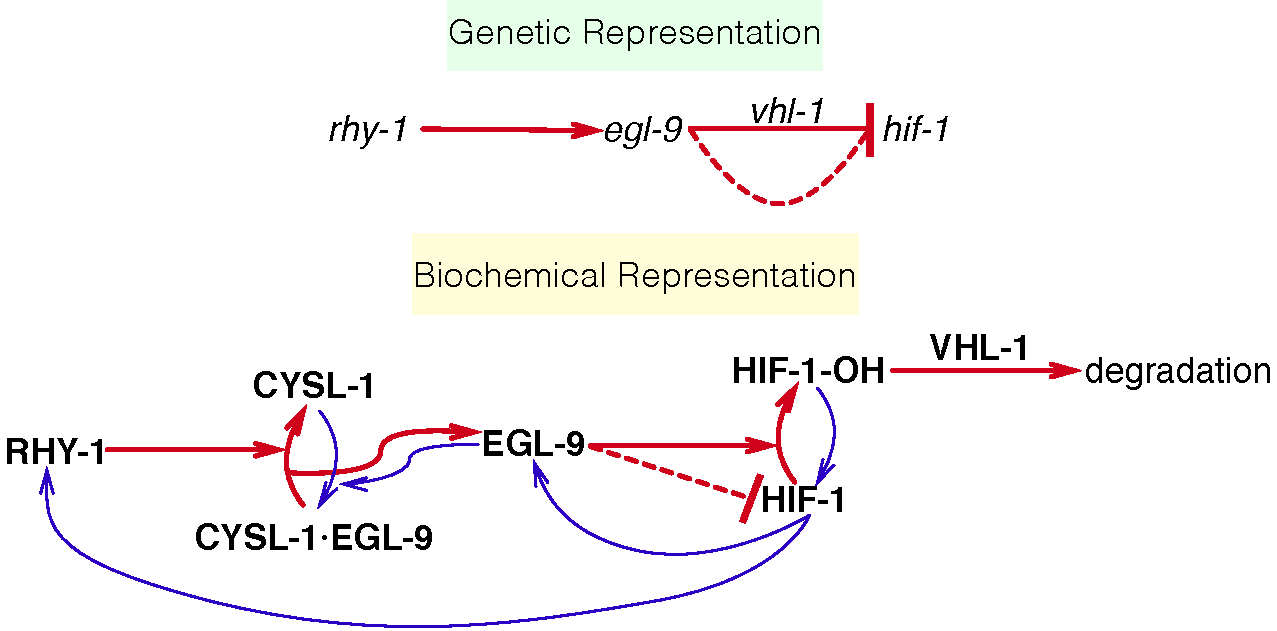
\includegraphics[width=.7\linewidth]{hypims/HIF1pathway.pdf}
\caption{
Genetic and biochemical representation of the hypoxia pathway in \cel{}.
Red arrows are arrows that lead to inhibition of \hifp{}, and blue arrows
are arrows that increase \hifp{} activity or are the result of \hifp{} activity.
\eglp{} is known to exert \gene{vhl-1}-dependent and independent repression
on \hifp{} as shown in the genetic diagram. The \gene{vhl-1}-independent
repression of \hifp{} by \eglp{} is denoted by a dashed line and is not dependent
on the hydroxylating activity of \eglp{}.
Technically, RHY-1 inhibits CYSL-1, which in turn inhibits EGL-9, but this
interaction was abbreviated in the genetic diagram for clarity.
}
\label{fig:pathway}
\end{figure}

Here, we show that transcriptomes contain robust signals that can be
used to infer relationships between genes in complex metazoans by reconstructing
the hypoxia pathway in \cel{} using RNA-seq.
Furthermore, we show that the phenomenon of phenotypic epistasis, a hallmark of
genetic interaction, holds at the molecular systems level.
We also demonstrate that transcriptomes contain sufficient information, under
certain circumstances, to order genes in a pathway using only single mutants.
Finally, we were able to identify genes that appear to be downstream of \gene{egl-9}
and \gene{vhl-1}, but do not appear to be targets of \gene{hif-1}.
Using a single set of genome-wide measurements, we were able to observe and
quantitatively assess  significant fraction of the known transcriptional
effects of \gene{hif-1} in \cel{}.
A complete version of the analysis, with ample documentation, is available at
\url{https://wormlabcaltech.github.io/mprsq}.

\section*{Results}
\subsection*{The hypoxia pathway controls thousands of genes in \cel{}}
\label{sub:summary}

We selected four single mutants within the hypoxia pathway for expression profiling:
\egl{} (\emph{sa307}), \rhy{} (\emph{ok1402}), \vhl{} (\emph{ok161}), \hif{} (\emph{ia4}).
We also sequenced the transcriptomes of two double mutants, \eglvhl{} (\emph{sa307},
\emph{ok161}) and \eglhif{} (\emph{sa307}, \emph{ia4}) as well as wild-type N2 as
a control sample. Each genotype  was sequenced in triplicate at a depth of 15
million reads. We performed whole-organism RNA-seq of these mutants at a moderate
sequencing depth ($\sim7$ million mapped reads for each individual replicate)
under normoxic conditions. For single samples, we identified around 22,000 different
isoforms per sample, which allowed us to measure differential expression of 18,344
isoforms across all replicates and genotypes (this constitutes  $\sim$70\% of
the protein coding isoforms in \cel{}).
We also included in our analysis a \fog{} (\emph{q71}) mutant which we have previously
studied~\citep{Angeles-Albores2016a}, because \gene{fog-2} is not reported to
interact with the hypoxia pathway.
We analyzed our data using a general linear model on
logarithm-transformed counts. Changes in gene expression are reflected in the
regression coefficient, $\beta$ which is specific to each isoform within a genotype.
Statistical significance is achieved when the q-values for each $\beta$ (p-values
adjusted for multiple testing) are less than 0.1. Genes that are significantly
altered between wild-type and a given mutant have $\beta$ values that are
statistically significantly different from 0.  These coefficients are not equal
to the average log-fold change per gene, although they are loosely related to
this quantity. Larger magnitudes of $\beta$ correspond to larger perturbations.
These coefficients can be used to study the RNA-seq data in question.

In spite of the moderate sequencing depth, transcriptome profiling of the hypoxia
pathway revealed that this pathway controls thousands of genes in \cel{}. The
\egl{} transcriptome showed differential expression of \egln{} genes. Similarly,
\rhyn{} genes were differentially expressed in \rhy{} mutants. The \vhl{}
transcriptome showed considerably fewer differentially expressed genes (\vhln{}),
possibly because it is a weaker controller of \hif{} than
\egl{}~\citep{Shao2009}. The \egl{};\vhl{} double mutant transcriptome showed
\eglvhln{} differentially expressed genes. The \hif{} mutant also showed a
transcriptomic phenotype involving \hifn{} genes. The \eglhif{} double mutant
showed a similar number of genes with altered expression (\eglhifn{} genes, see
Table~\ref{tab:genes}).

\begin{table}[tbhp]
  \centering
  \begin{tabular}{lr}
    \toprule{}
    Genotype & Differentially Expressed Genes \\
    \midrule{}
    \egl{} & \egln{}\\
    \rhy{} & \rhyn{}\\
    \vhl{} & \vhln{}\\
    \eglvhl{} & \eglvhln{}\\
    \eglhif{} & \eglhifn{}\\
    \fog{} & \fogn{}\\
    \bottomrule{}
  \end{tabular}
  \caption{Number of differentially expressed genes in each mutant.}
\label{tab:genes}
\end{table}

\subsection*{Principal Component Analysis visualizes epistatic relationships between genotypes}
\label{sub:Clustering}

Principal Component Analysis (PCA) is a well-known technique in bioinformatics that is
used to identify relationships between high dimensional data points~\citep{Yeung2001}
We performed PCA on our data to examine whether each genotype clustered in a biologically
relevant manner. PCA identifies the vector that can explain most of the variation
in the data;this is called the first PCA dimension. Using PCA, one can identify
the first $n$ dimensions that can explain more than 95\% of the variation in the
data. Sample clustering in these $n$ dimensions often indicates biological
relationships between the data, although interpreting PCA dimensions can be
difficult.

After applying PCA, we expected \hif{} to cluster near \eglhif{}, because
\hif{} exhibits no phenotypic defects under normoxic conditions, in contrast to
\egl{}, which exhibits an egg-laying (Egl) phenotype in the same environment.
In \eglhif{} mutants the Egl phenotype of \egl{} mutants is suppressed and instead
the grossly wild-type phenotype of \hif{} is observed. On the other hand, we
expected \egl{}, \rhy{}, \vhl{} and \eglvhl{} to form a separate cluster since
each of these genotypes is Egl and has a constitutive hypoxic response. Finally,
we included as a negative control a \fog{} mutant we have analyzed
previously~\citep{Angeles-Albores2016a}. This data was obtained at a different
time from the other genotypes, so we included a batch-normalization term in our
equations to account for this. Since \gene{fog-2} has not been described
to interact with the hypoxia pathway, we expected that it should appear far away
from either cluster.

The first dimension of the PCA analysis was able to discriminate between mutants
that have constitutive high levels of \hifp{} and mutants that have no \hifp{},
whereas the second dimension was able to discriminate between mutants within the
hypoxia pathway and outside the hypoxia pathway (see Fig.~\ref{fig:pca}).
Therefore expression profiling measures enough signal to cluster genes in a
meaningful manner in complex metazoans.

\begin{figure}[tbhp]
\centering
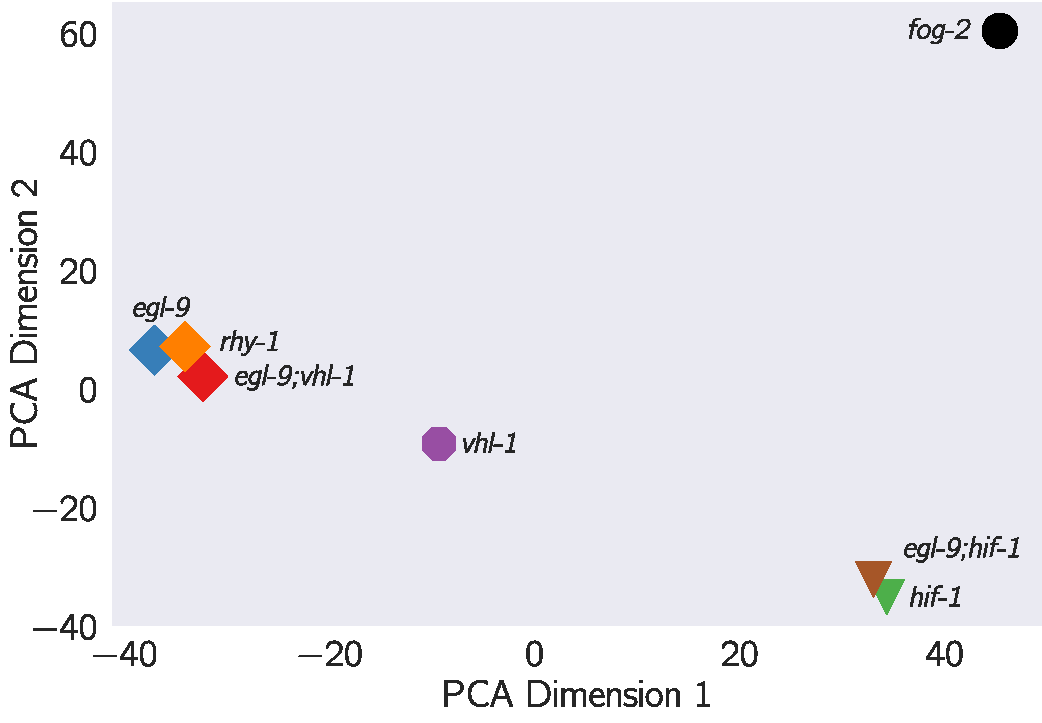
\includegraphics[width=0.5\linewidth]{hypims/pca.pdf}
\caption{
Principal component analysis of various \cel{} mutants. Genotypes that have an
activated hypoxia response (\emph{i.e}, \egl{}, \vhl{}, and \rhy{}) cluster far
from \hif{}. \hif{} clusters with the suppressed \eglhif{} double mutant.
The \fog{} transcriptome, used as an outgroup, is far away from either cluster.
}
\label{fig:pca}
\end{figure}

\subsection*{Reconstruction of the hypoxia pathway from first genetic principles}
\label{sec:reconstruct}
Having shown that the signal in the mutants we selected was sufficient to
cluster mutants using the values of the regression coefficients $\beta$, we set
out to reconstruct the hypoxia pathway from genetic first principles. In general,
to reconstruct a pathway, we must first assess whether two genes act on the same
phenotype. If they do not act on the same phenotype (the set of commonly differentially
regulated genes between two mutants is empty), these mutants are independent.
If they are not independent, then two mutants have a shared transcriptomic
phenotype (STP)---a set of genes or isoforms that are differentially expressed in
both mutants, without taking into account what direction they change in. In this
case, we must measure whether these genes act additively or epistatically on the
measured phenotype; if there is epistasis we must measure whether it is
positive or negative, in order to assess whether the epistatic relationship is a
genetic suppression or a synthetic interaction.

\subsubsection*{Genes in the hypoxia mutant act on the same transcriptional phenotype}
\label{sec:phenotypes}
We observed that all the hypoxia mutants had significant shared transcriptomic
phenotypes (fraction of the transcriptomes that was shared between mutants
ranged from a minimum of 6.8\% shared between \hif{} and \eglvhl{} to a maximum
of 31\% shared genes between \egl{} and \eglvhl{}). For comparison, we also
analyzed a previously published \fog{} transcriptome~\citep{Angeles-Albores2016a}.
The \gene{fog-2} gene is involved in masculinization of the \cel{} germline,
which enables sperm formation, and is not known to be involved in the hypoxia
pathway. The hypoxia pathway mutants and the \fog{} mutant also showed shared
transcriptomic phenotypes (3.6\%--12\% genes), but correlations between
expression level changes were considerably weaker (see below), suggesting that
there is minor cross-talk between these pathways.


% genetic correlations
\begin{figure}[tbhp]
\centering
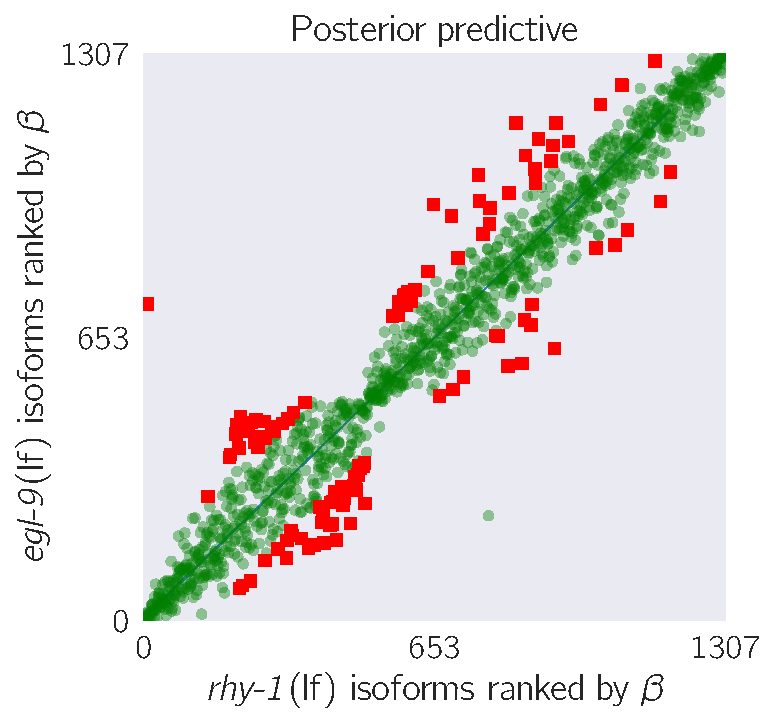
\includegraphics[width=.4\linewidth]{hypims/multiplemodes-eb.pdf}
\caption{
Strong transcriptional correlations can be identified between genes
that share a positive regulatory connection. We took the \egl{} and the \rhy{}
transcriptomes, identified differentially expressed genes common to both
transcriptomes and ranked each gene according to its differential expression
coefficient $\beta$. We plotted the rank of each gene in \rhy{} versus the
rank of the same gene in the \egl{} transcriptome. The result is an almost
perfect correlation. Green, transparent large points mark inliers to the primary
regressions (blue lines); red squares mark outliers to the primary regressions.
}
\label{fig:genetic_interactions}
\end{figure}

We wanted to know whether it was informative to look at quantitative agreement
within STPs. For each mutant pair, we rank-transformed
the regression coefficients $\beta$ of each isoform within the STP, and
calculated lines of best fit using Bayesian regression with a Student-T
distribution to mitigate noise from outliers and plotted the results in a rank plot
(see Fig~\ref{fig:genetic_interactions}). For transcriptomes associated with the
hypoxia pathway, we found that these correlations tended to have
values higher than 0.9 with a tight distribution around the line of best fit.
The correlations for mutants from the hypoxia pathway
with the \fog{} mutant were considerably weaker, with magnitudes between
0.6--0.85 and greater variance around the line of best fit.
Although \gene{hif-1} is known to be genetically repressed by \gene{egl-9}, \gene{rhy-1} and
\gene{vhl-1}~\citep{Epstein2001,Shen2006}, all the correlations
between mutants of these genes and \hif{} were positive.

After we calculated the pairwise correlation within each STP,
we weighted the result of each regression by the
number of isoforms within the STP and
divided by the total number of differentially expressed isoforms present in the
two mutant transcriptomes that contributed to that specific STP,
$N_\mathrm{overlap}/N_{\mathrm{g_1} \cup \mathrm{g2}}$.
The weighted regressions recapitulated a module network (see Fig.~\ref{fig:heatmap}).
We identified a strong positive interaction between \egl{} and \rhy{}.
The magnitude of this weighted correlation derives from the magnitude of the
transcriptomes for these mutants (\egln{} and \rhyn{} differentially expressed
genes respectively) and the overlap between both genes was
extensive, which makes the weighting factor considerably larger than other pairs.
The weak correlation between \hif{} and \egl{} results from the small size of
the \hif{} transcriptome and the small overlap between the transcriptomes.

The fine-grained nature of transcriptional phenotypes means that these weighted
correlations between transcriptomes of single mutants are predictive of genetic
interaction.

% heatmap
\begin{figure}[tbhp]
\centering
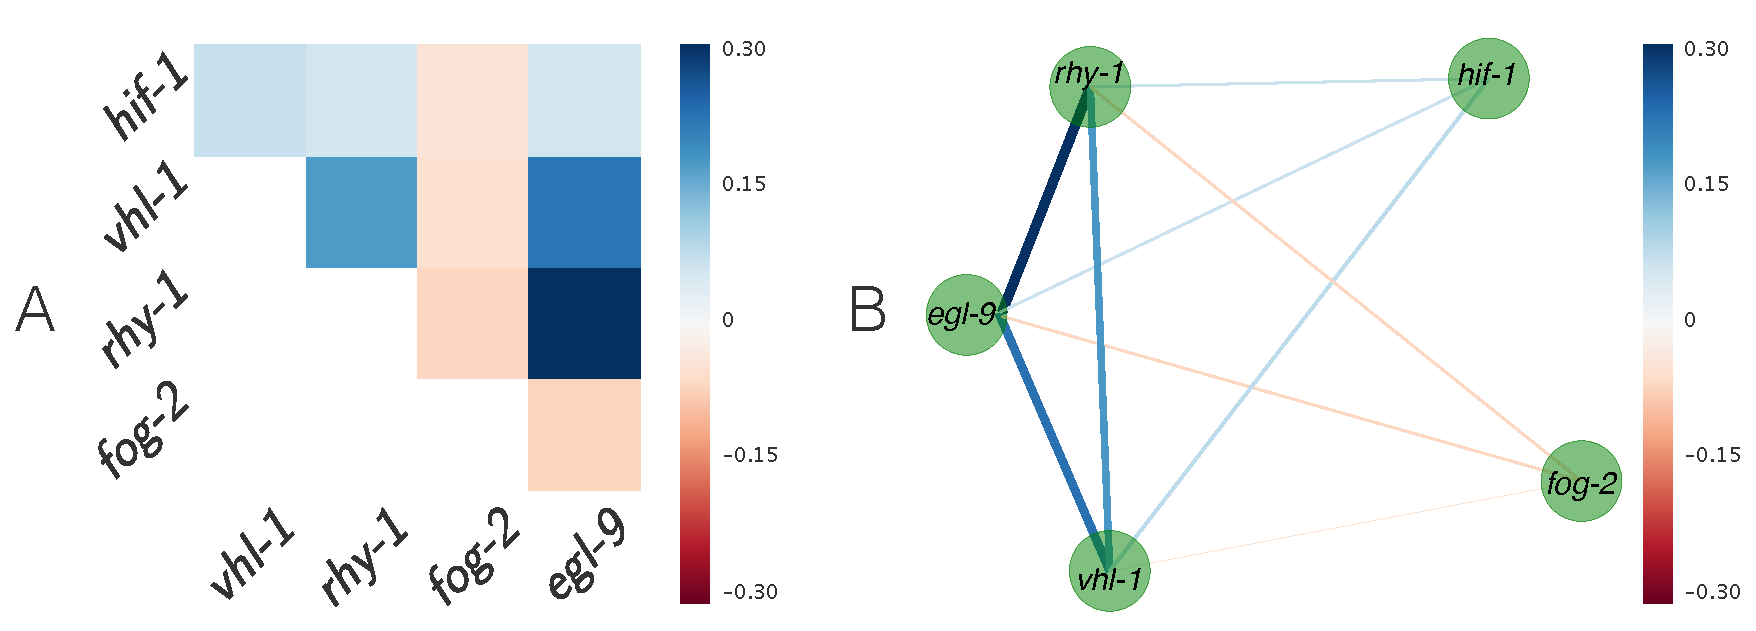
\includegraphics[width=\linewidth]{hypims/bayesian-heatmap-horizontal.pdf}
\caption{
\textbf{A}. Heatmap showing pairwise regression values between all
single mutants. \textbf{B}. Correlation network drawn from \textbf{A}. Edge
width is proportional to the logarithm of the magnitude of the weighted
correlation between two nodes divided by absolute value of the weighted
correlation value of smallest magnitude. Edges are also colored according to the
heatmap in \textbf{A}. Inhibitors of \gene{hif-1} are tightly correlated and form
a control module;
\gene{hif-1} is positively correlated to its inhibitors, albeit weakly;
and
\gene{fog-2}, a gene that is not reported to interact with the hypoxia pathway,
has the smallest, negative correlation to any gene.
}
\label{fig:heatmap}
\end{figure}

\subsubsection*{A quality check of the transcriptomic data reveals excellent agreement
            with the literature}
\label{sub:quality_check}
One way to establish whether genes are acting additively or epistatically to each
other is to perform qPCR of a reporter gene in the single and double mutants. This
approach was used to successfully map the relationships within the hypoxia
pathway (see, for example~\citep{Shao2009,Shen2006}). A commonly used hypoxia reporter
gene is \nhr{}, which is known to exhibit a several-fold increase in mRNA
expression when \hifp{} accumulates~\citep{Shen2006,Shen2005,Park2012}. Likewise,
increased \hifp{} fucntion is known to cause increased of \gene{rhy-1}
and \gene{egl-9}~\citep{Powell-Coffman2010}.

We can
selectively look at the expression of a few genes at a time. Therefore, we
queried the changes in expression of \gene{rhy-1}, \gene{egl-9}, and \nhr{}. We
included the nuclear laminin gene \lam{} as a representative negative control not
believed to be responsive to alterations in the hypoxia pathway.
\nhr{} was upregulated in \egl{}, \rhy{} and \vhl{}, but remains unchanged in \hif{}.
\eglvhl{} had an expression level similar to \egl{}; whereas the
\eglhif{} mutant showed wild-type levels of the reporter expression, as reported
previously~\citep{Shen2006} (see Fig.~\ref{fig:qpcr}).

% in silico qPCR
\begin{figure}[tbhp]
\centering
\includegraphics[width=.5\linewidth]{hypims/qpcr.pdf}
\caption{
\textbf{Top}: Observed $\beta$ values of select genes. We selected
four genes (\gene{rhy-1}, \gene{egl-9}, \nhr{} and \lam{}, shown on the x-axis)
and plotted their regression coefficients, $\beta$, as measured for every
genotype (represented by one of six colors) to study the epistatic relationships
between each gene. Asterisks above a bar represent a regression coefficient
statistically significantly different from 0 (\qval{1}) relative to a wild-type
control. Error bars show standard error of the mean
value of $\beta$. \nhr{} is an expression reporter that has been used previously
to identify \gene{hif-1} regulators~\citep{Shen2006,Shao2009}. \lam{} is shown here
as a negative control that should not be altered by mutations in this pathway.
We measured modest increases in the levels of \gene{rhy-1} mRNA when \hif{} is
knocked out.
}
\label{fig:qpcr}
\end{figure}

We observed changes in \rhy{} expression consistent with previous
literature~\citep{Shen2006} when \hifp{} accumulates.
We also observed increases in \gene{egl-9} expression in \egl{}.
\gene{egl-9} is known as a hypoxia responsive gene~\citep{Powell-Coffman2010}.
Although changes in \gene{egl-9} expression were not statistically significantly
different from the wild-type in
\rhy{} and \vhl{} mutants, the mRNA levels of \gene{egl-9} still trended towards
increased expression in these genotypes.
As with \nhr{}, \gene{egl-9} and \gene{rhy-1} expression were wild-type in
\eglhif{} and \eglvhl{} mutant showed expression phenotypes identical to \egl{}.
This dataset also showed that knockout of \gene{hif-1} resulted in a modest
increase in the levels of \gene{rhy-1}. This suggests that \gene{hif-1}, in
addition to being a positive regulator of \gene{rhy-1}, also inhibits it, which
constitutes a novel observation.
Using a single reporter we would have been able to reconstruct an
important fraction of the genetic relationships between the genes in the hypoxia
pathway–--but would likely fail to observe yet other genetic interactions, such as
the evidence for \gene{hif-1} negatively regulating \gene{rhy-1} transcript levels.


\subsection*{Transcriptome-wide epistasis}
Ideally, any measurement of transcriptome-wide epistasis should conform to certain
expectations. First, it should make use of the regression coefficients of as
many genes as possible. Second, it should be summarizable in a single,
well-defined number. Third, it should have an intuitive behavior, such that
special values of the statistic should each have an unambiguous interpretation.

One way of displaying transcriptome-wide epistasis is to plot transcriptome data onto
an epistasis plot (see Fig~\ref{fig:egl9epistasis}). In an epistasis plot, the
X-axis represents the expected expression of a double mutant $a^-b^-$ if $a$
and $b$ interact additively.
In other words, each individual isoform's x-coordinate is the sum of the regression
coefficients from the single mutants $a^-$ and $b^-$.
The Y-axis represents the deviations from the additive (null) model, and
can be calculated as the difference between the observed regression coefficient
and the predicted regression coefficient. Only genes that are differentially
expressed in all three genotypes are plotted. Assuming that the two genes interact
via a simple phenotype (for example, if both genes affect a transcription factor
that generates the entire transcriptome), these plots will generate specific
patterns that can be described through linear regressions. The slope of these
lines, $s_{a,b}$, is the transcriptome-wide epistasis coefficient.

Epistasis plots can be understood intuitively for simple cases of genetic
interactions. If two genes act additively on the same set of differentially expressed
isoforms then all the plotted points will fall along the line $y=0$.
If two genes interact in an unbranched pathway, then $a^-$ and $b^-$ should
have identical phenotypes for $a^-$, $b^-$ and $a^-b^-$, if all the genotypes are
homozygous for genetic null alleles~\citep{Huang2006}. It follows that the
data points should fall along a line with slope equal to $-\frac{1}{2}$. On the
other hand, in the limit of complete inhibition of $a$ by $b$, the plots should show
a line of best fit with slope equal to $-1$\footnote{Specifically, this follows
from assuming that $b^-$ is wild-type under the conditions assayed; and
$a^-b^-$ = $b^-$ = wild-type}.
Genes that interact synthetically (\emph{i.e.}, through an OR-gate) will fall
along lines with slopes $>0$. When there is epistasis of one gene over another,
the points will fall along a line of best fit with slope $s_{ab=b}$ or $s_{ab=a}$.
This slope must be determined from the single-mutant data.
From this information, we can use the single mutant data to predict the
distribution of slopes that results for each case stated above, as well as for
each epistatic combination ($a^-b^-=a^-$ or $a^-b^-=b^-$). The transcriptome-wide
epistasis coefficient ($s_{a, b}$), emerges as a powerful way to quantify epistasis
because it integrates information from many different genes or isoforms into a
single number (see Fig.~\ref{fig:egl9epistasis}).

In our experiment, we studied two double mutants, \eglhif{} and \eglvhl{}.
We wanted to understand how well an epistasis analysis based on transcriptome-wide
coefficients agreed with the epistasis results reported in the literature, which
were based on qPCR of single genes. Therefore, we performed orthogonal distance
regression on the two gene combinations we studied (\gene{egl-9} and
\gene{vhl-1}; and \gene{egl-9} and \gene{hif-1}) to determine the epistasis
coefficient for each gene pair. We also generated models for the special cases
mentioned above (additivity, $a^-b^-=a^-$, strong suppression, etc\ldots) using
the single mutant data. For every simulation, as well as for the observed data,
we used bootstraps to generate probability distributions of the epistasis
coefficients.

When we compared the predictions for the transcriptome-wide epistasis coefficient,
$s_{egl-9,vhl-1}$ under different assumptions with the observed slope ($-0.42$). We
observed that the predicted slope matched the simulated slope for the case where
\gene{egl-9} is epistatic over \gene{vhl-1} (\egl{} = \eglvhl{}, see
Fig.~\ref{fig:egl9epistasis}) and did not overlap with any other prediction.
Next, we predicted the distribution of $s_{egl-9,hif-1}$ for different pathways
and contrasted with the observed slope. In this case, we saw that the uncertainty
in the observed coefficient overlapped significantly with the strong suppression
model, where \eglp{} strongly suppresses \hifp{}, and also with the model where
\hif{} = \eglhif{}. In this case, both models are reasonable---\hifp{} is strongly
suppressed by \eglp{}, and we know from previous literature that the epistatic
relationship, \hif{} = \eglhif{}, is true for these mutants. In fact, as the
repression of \hifp{} by \eglp{} becomes stronger, the epistatic model should converge
on the limit of strong repression (see
\href{https://wormlabcaltech.github.io/mprsq/analysis_notebooks/epistasis_6.html}
{Epistasis}).

Another way to test which model best explains the epistatic relationship between
\gene{egl-9} and \gene{vhl-1} is to use Bayesian model selection to calculate
an odds ratio between two models to explain the observed data. Models can be placed
into two categories: parameter-free and fit. Parameter free models are `simpler'
because their parameter space is smaller (0 parameters) than the fit models ($n$
parameters). By Occam's razor, simpler models should be preferred to more
complicated models. However, simple models suffer from the drawback that
systematic deviations from them cannot be explained or accomodated, whereas more
complicated models can alter the fit values to maximize their explanatory power.
In this sense, more complicated models should be preferred when the data shows
systematic deviations from the simple model. Odds-ratio selection gives us a way
to quantify the trade-off between simplicity and explanatory power.

We reasoned that comparing a fit model ($y = \alpha\cdot x$, where $\alpha$ is
the slope of best fit) against a parameter-free model ($y = \gamma\cdot x$,
where $\gamma$ is a single number) constituted a conservative approach towards
selecting which theoretical model (if any) best explained the data. In particular,
this approach will tend to strongly favor the line of best fit over simpler model
for all but very small, non-systematic deviations. We decided
that we would reject the theoretical models only if the line of best-fit
was $10^3$ times more likely than the theoretical models (odds ratio, OR $>10^3$).
Comparing the odds-ratio between the line of best fit and the different pathway
models for \gene{egl-9} and \gene{vhl-1} showed similar results to the simulation.
Only the theoretical model \egl{} = \eglvhl{} could not be rejected (OR = 0.46),
whereas all other models were significantly less likely than the line of best fit
(OR $>10^{44}$).
Therefore, \gene{egl-9} is epistatic to \gene{vhl-1}. Moreover,
since $s_{egl-9, vhl-1}$ is strictly between and not equal to $0$ and $-0.5$, we
conclude that \gene{egl-9} acts on its transcriptomic phenotype in
\gene{vhl-1}-dependent and independent manners. A branched pathway that can lead
to epistasis coefficients in this range is a pathway where \gene{egl-9} interacts
with its transcriptomic phenotype via branches that have the same valence (both
positive or both negative)~\citep{Shao2009}. When we performed a similar analysis
to establish the epistatic relationship between \gene{egl-9} and \gene{hif-1},
we observed that the best alternative to a free-fit model was a model where
\gene{hif-1} is epistatic over \gene{egl-9} (OR$=2551$), but the free-fit model
was still preferred. All other models were strongly rejected (OR $>10^{25}$).

% epistasis graph
\begin{figure}[tbhp]
\centering
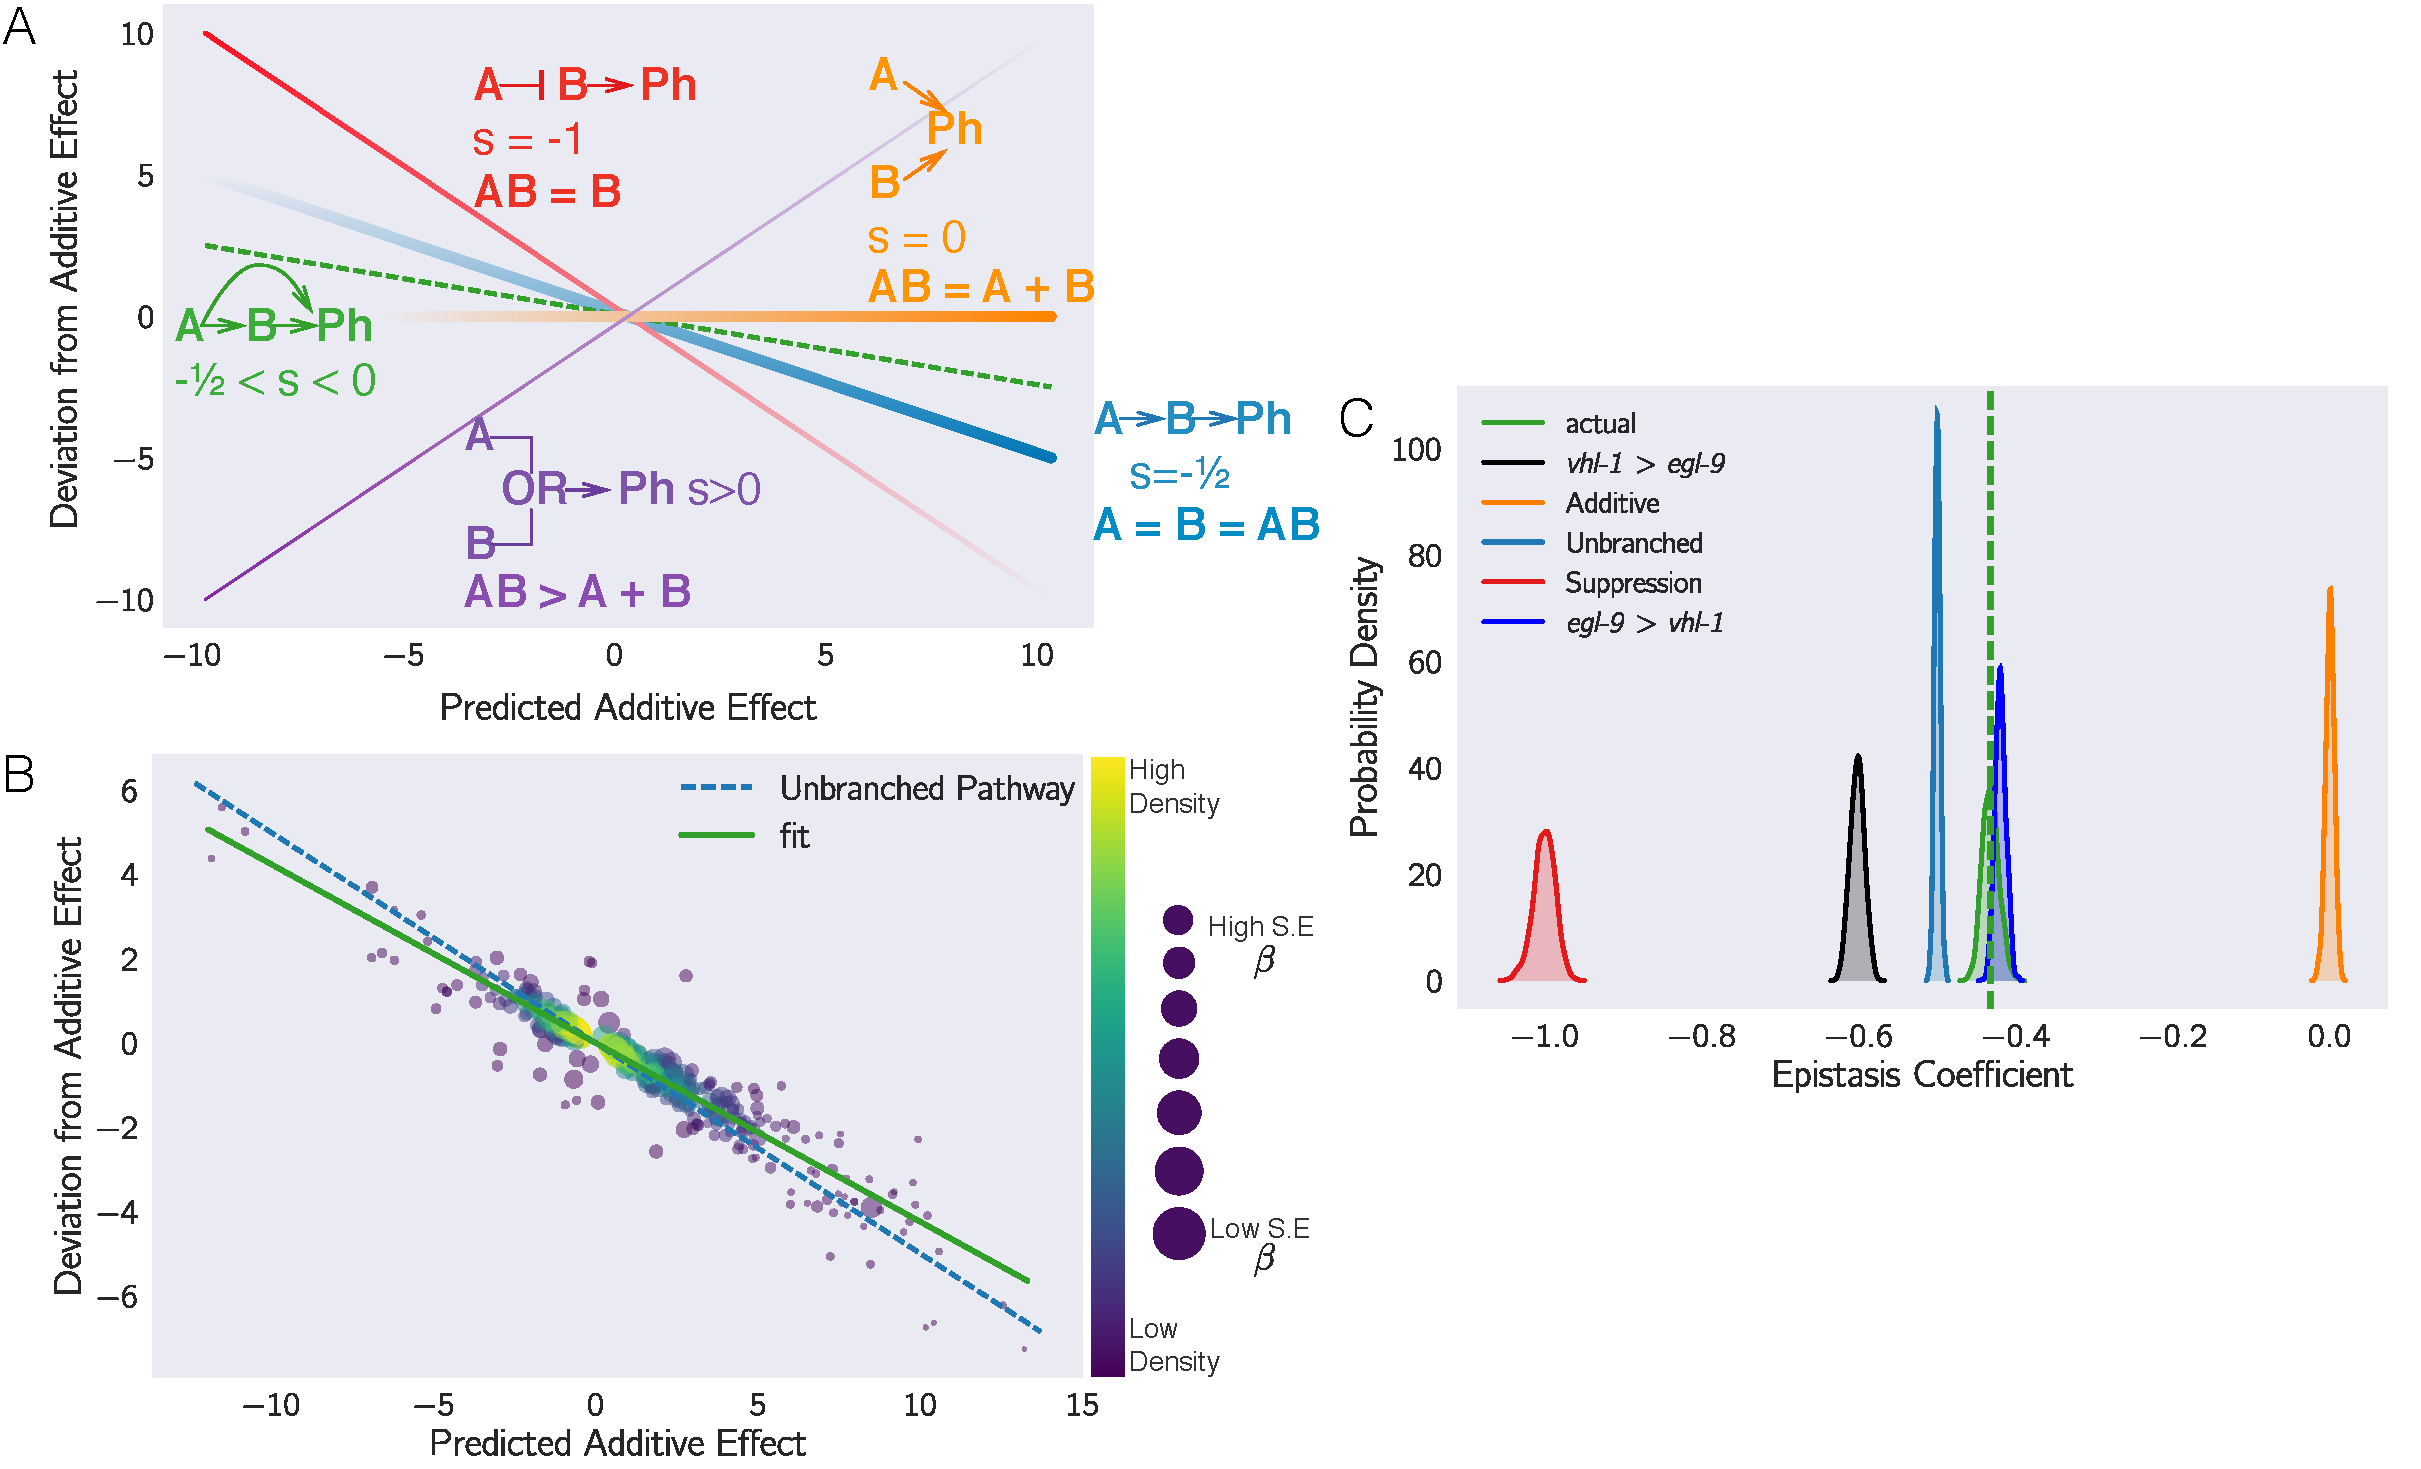
\includegraphics[width=\linewidth]{hypims/egl9hif1-epistasis-horizontal.pdf}
\caption{
(\textbf{A}) Schematic diagram of an epistasis plot. The X-axis on an epistasis
plot is the expected coefficient for a double mutant under an additive model
(null model). The Y-axis plots deviations from this model. Double mutants that
deviate in a systematic manner from the null model exhibit transcriptome-wide epistasis
($s$). To measure $s$, we perform a linear regression on the data. The slope of
the line of best fit is $s$. This coefficient is related to genetic architectures.
Genes that act additively on a phenotype \textbf{(Ph)} will have $s=0$ (orange
line); whereas
genes that act along an unbranched pathway will have $s=-1/2$ (blue line).
Strong
repression is reflected by $s=-1$ (red line). Cases where $s>0$ correspond to
synthetic interactions (purple line), and in the limit as $s\rightarrow\infty$,
the synthetic interaction
must be an OR-gate. Cases where $0 < s < -1/2$ correspond to circuits
that have multiple positive branches; whereas cases where
$-1/2<s< -1$ correspond to cases where the branches have different valence.
Cases where $s < -1$ represent inhibitory branches.
(\textbf{B}) Epistasis plot showing
that the \eglvhl{} transcriptome deviates significantly from a null additive.
Points are colored qualitatively according to density (purple---low,
yellow---high) and size is inversely proportional to the standard
error (S.E.) of the y-axis (larger points, higher accuracy). The purple line
is the line of best fit from an orthogonal distance regression.
(\textbf{C}) Comparison of simulated epistatic coefficients against the observed
coefficient. Green curve shows the bootstrapped observed transcriptome-wide epistasis
coefficient for \gene{egl-9} and \gene{vhl-1}. Dashed green line shows the mean
value of the data. Using the single mutants, we simulated coefficient
distributions for a linear model (light blue, centered at $-0.5$);
an additive model (orange, centered at 0); a model where either
\gene{egl-9} or \gene{vhl-1} masks the other phenotype (dark blue and black,
respectively) and a complete suppression model (red, centered at $-1$).
The observed coefficient overlaps the predicted epistasis curve for
\eglvhl{} = \egl{} (green and dark blue).
}
\label{fig:egl9epistasis}
\end{figure}

\subsubsection*{Epistasis can be predicted}
Given our success in measuring epistasis coefficients, we wanted to know whether
we could predict the epistasis coefficient between \gene{egl-9} and \gene{vhl-1}
in the absence of the \egl{} genotype. Since \rhyp{} indirectly activates
\eglp{}, the \rhy{} transcriptome should contain more or less
equivalent information to the \egl{} transcriptome. Therefore, we generated
predictions of the epistasis coefficient between \gene{egl-9} and \gene{vhl-1}
by substituting in the \rhy{} data. We predicted $s_{rhy-1,vhl-1} = -0.45$.
Similarly, we used the \eglvhl{} double mutant to
measure the epistasis coefficient while replacing the \egl{} dataset with the \rhy{}
dataset. We found that the epistasis coefficient using this substitution was $-0.40$.
This coefficient was different from $-0.50$ (OR $>10^{62}$), reflecting the same
qualitative conclusion that the hypoxia pathway is branched.
In conclusion, we were able to obtain a quantitatively close prediction of the
epistasis coefficient for two mutants using the transcriptome of a related,
upstream mutant. Finally, we showed that in the absence of a single mutant, an
upstream locus can under some circumstances be used to estimate epistasis
between two genes.


\subsection*{Transcriptomic decorrelation can be used to infer functional distance}
\label{sub:decorrelation}
% What are functional interactions?
So far, we have shown that RNA-seq can accurately measure genetic interactions.
However, genetic interactions are far removed from biochemical interactions:
Genetic interactions do not require two gene products to interact physically, nor
even to be physically close to each other. RNA-seq cannot measure physical
interactions between genes, but we wondered whether expression profiling contains
sufficient information to order genes along a pathway.

Single
genes are often regulated by multiple independent sources. The connection between
two nodes can in theory be characterized by the strength of the edges connecting
them (the thickness of the edge); the sources that regulate both
nodes (the fraction of inputs common to both nodes); and the genes that are
regulated by both nodes (the fraction of outputs that are common to both nodes).
In other words, we expected that expression profiles associated with a pathway
would respond quantitatively to quantitative changes in activity of the pathway.
Targeting a pathway at multiple points would lead to expression profile
divergence as we compare nodes that are separated by more degrees of freedom,
reflecting the flux in information between them.

% decorrelation
\begin{figure}[tbhp]
\centering
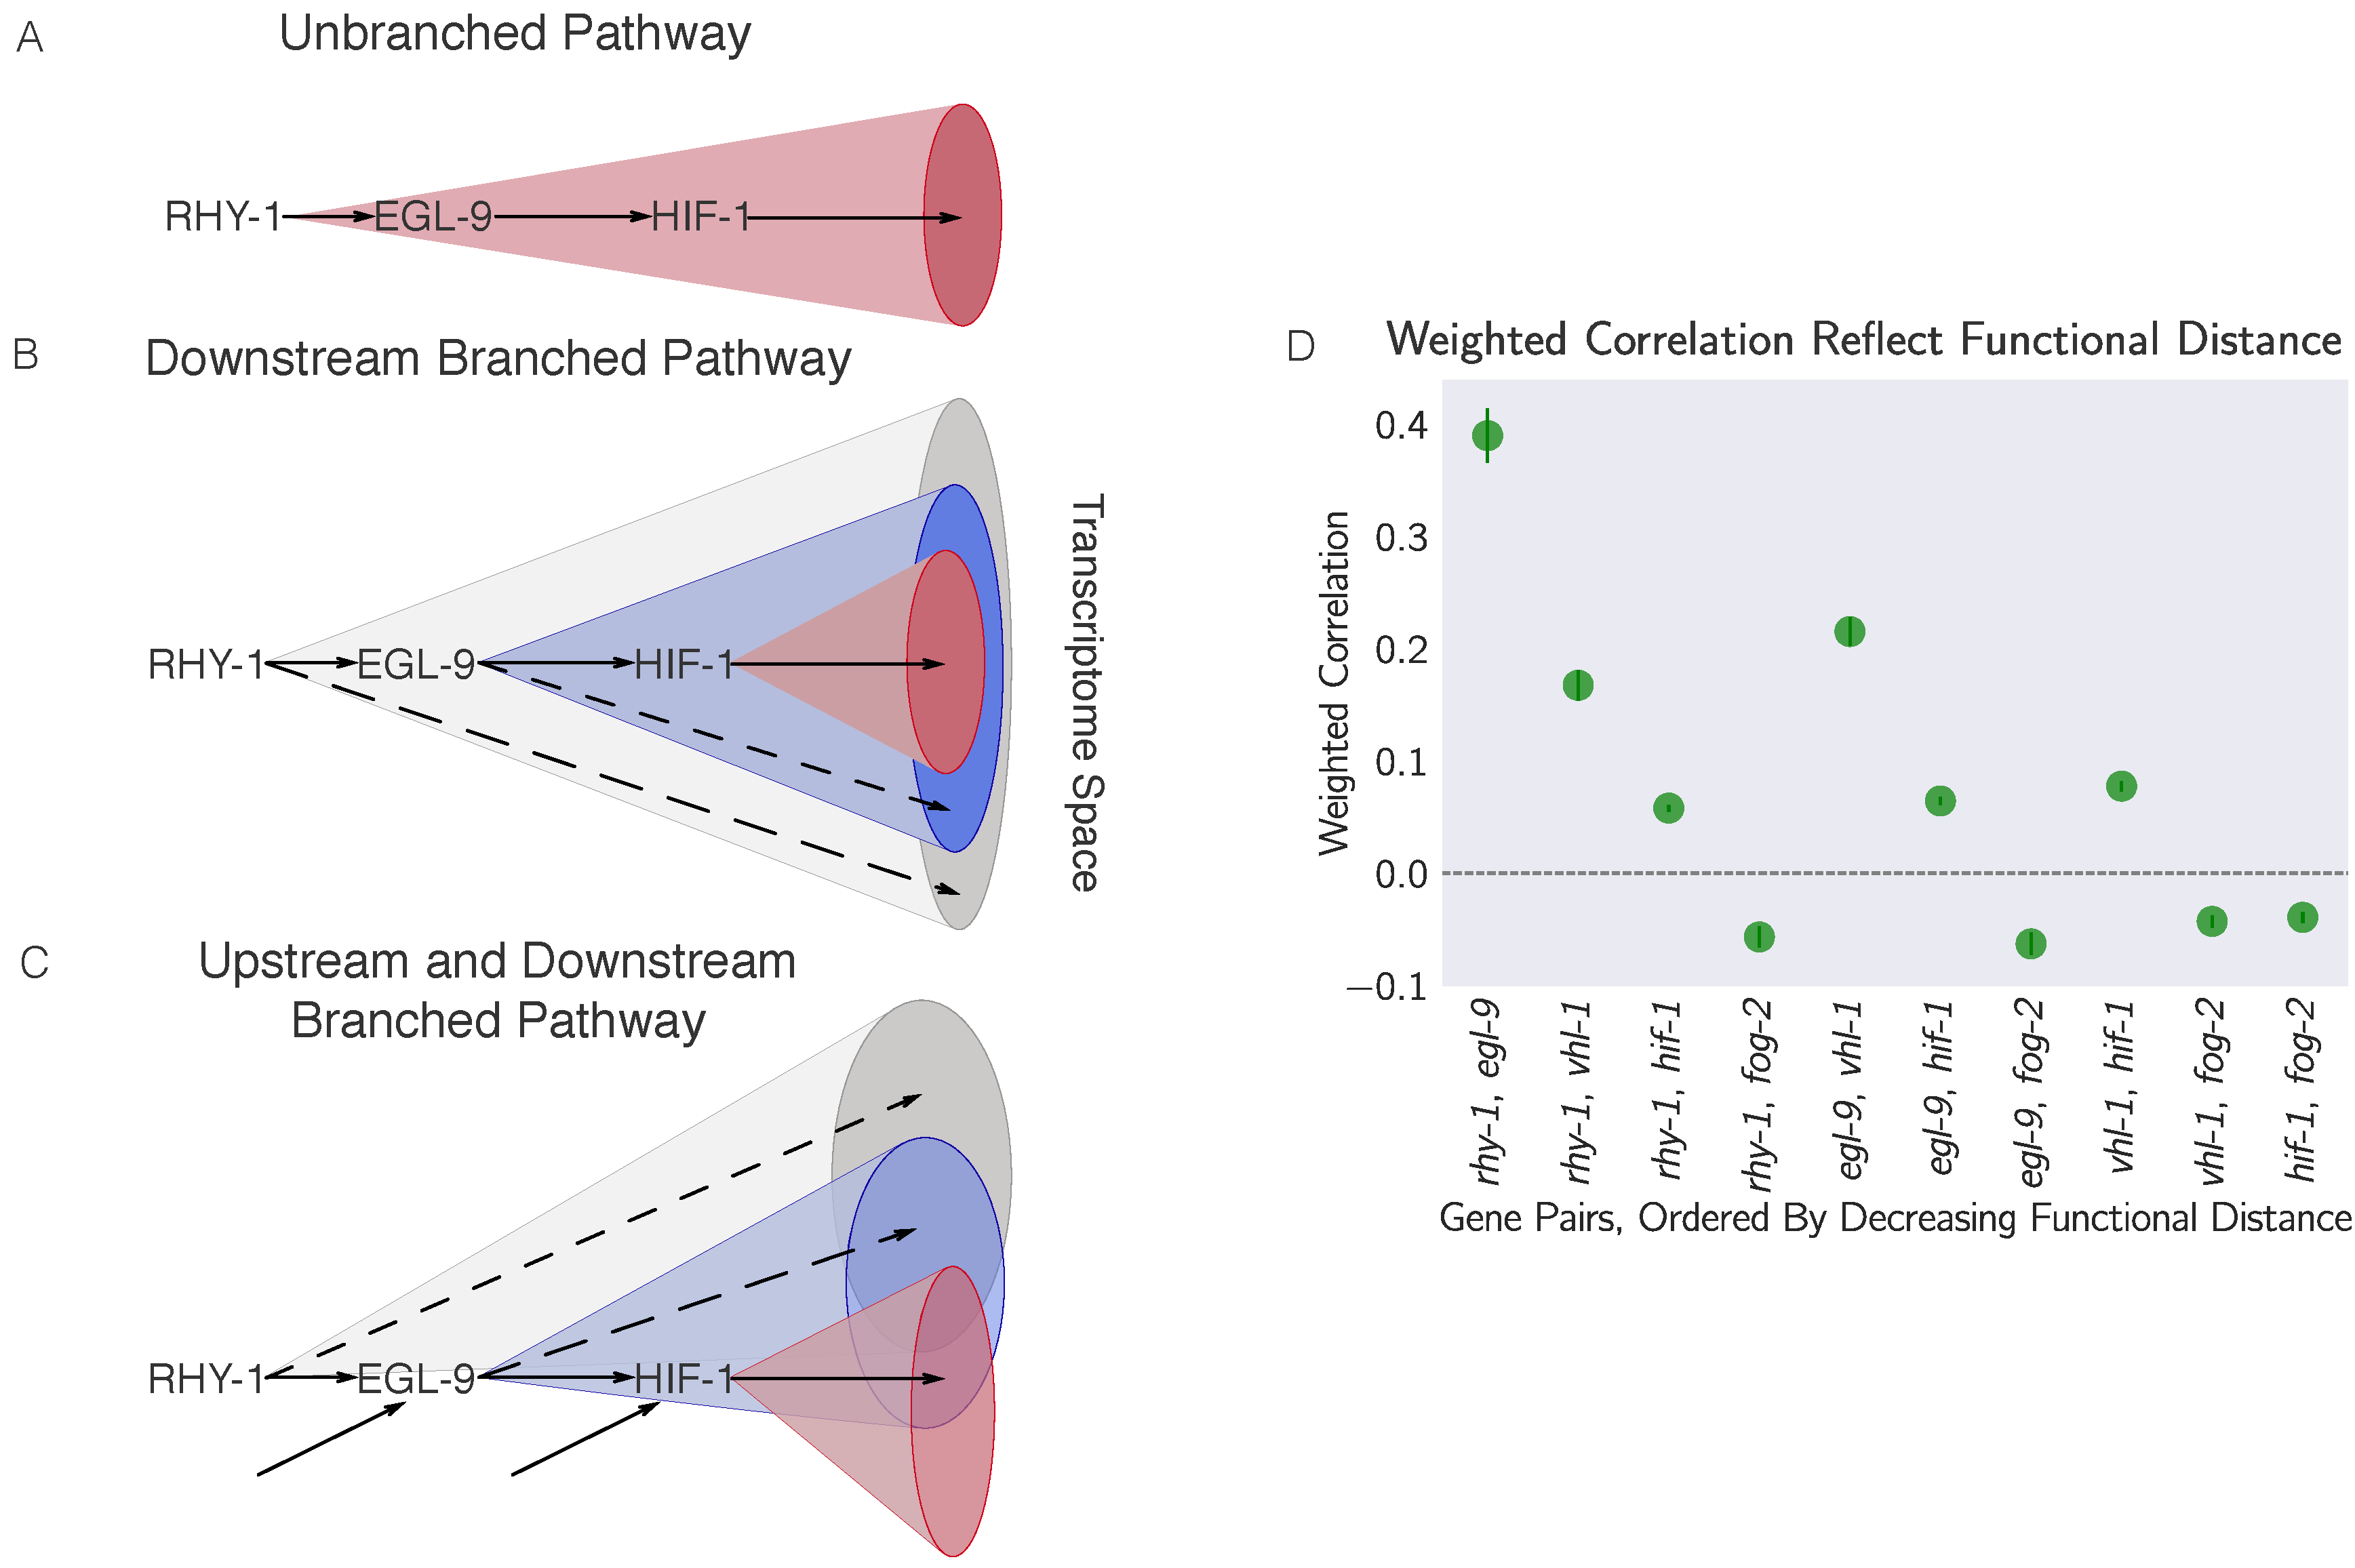
\includegraphics[width=.8\linewidth]{hypims/decorrelation-horizontal.pdf}
\caption{
Theoretically, transcriptomes can be used to order genes in a pathway under
certain assumptions. Arrows in the diagrams above are intended to show the
direction of flow, and do not indicate valence.
\textbf{A}. A linear pathway in which \gene{rhy-1} is the only gene controlling
\gene{egl-9}, which in turn controls \gene{hif-1} does not contain information
to infer the order between genes.
\textbf{B}. If \gene{rhy-1} and \gene{egl-9} have transcriptomic effects that are
separable from \gene{hif-1}, then the \gene{rhy-1} transcriptome should contain
contributions from \gene{egl-9}, \gene{hif-1} and \gene{egl-9}- and
\gene{hif-1}-independent pathways. This pathway contains enough information to
infer order.
\textbf{C}. If a pathway is branched both upstream and downstream,
transcriptomes will show even faster decorrelation. Nodes that are
separated by many edges may begin to behave almost independently of each other
with marginal transcriptomic overlap or correlation.
\textbf{D}. The hypoxia pathway can be ordered.
We hypothesize the rapid decay in correlation is due to a mixture of
upstream and downstream branching that happens along this pathway. Bars show the
standard error of the weighted coefficient from the Monte Carlo Markov Chain
computations.
}
\label{fig:decorrelation}
\end{figure}


We investigated the possibility that transcriptomic signals do in fact contain
relevant information about the degrees of separation by weighting the robust
Bayesian regression between each pair of genotypes by the size of the shared
transcriptomic phenotype of each pair divided by the total number of isoforms
differentially expressed in either mutant
($N_\mathrm{Intersection}/N_{\mathrm{Union}}$). We plotted the weighted
correlation of each gene pair, ordered by increasing functional distance
(see Fig.~\ref{fig:decorrelation}). In every case, we see that the weighted
correlation decreases monotonically due mainly, but not exclusively, to a smaller
STP.\@ We believe that this result is not due to random noise or insufficiently
deep sequencing. Instead, we propose a framework in which every gene is regulated
by multiple different molecular species, which induces progressive decorrelation.
This decorrelation in turn has two consequences. First, decorrelation within a
pathway implies that two nodes may be almost independent of each other if the
functional distance between them is large. Second, it may be possible to use
decorrelation dynamics to infer gene order in a branching pathway, as we have
done with the hypoxia pathway.

\subsection*{The circuit topology of the hypoxia pathway explains patterns in
            the data}
\label{sub:topology}
We noticed that while some of the rank plots contained a clear positive correlation
(see Fig.~\ref{fig:genetic_interactions}), other rank plots showed
a discernible cross-pattern (see Fig.~\ref{fig:xpattern}). In particular, this
cross-pattern emerged between \vhl{} and \rhy{} or between \vhl{} and \egl{},
even though genetically \gene{vhl-1}, \gene{rhy-1} and \gene{egl-9} are all
inhibitors of \hif{}. Such cross-patterns could be indicative of feedback loops
or other complex interaction patterns.

% correlative genetics again
\begin{figure}[tbhp]
\centering
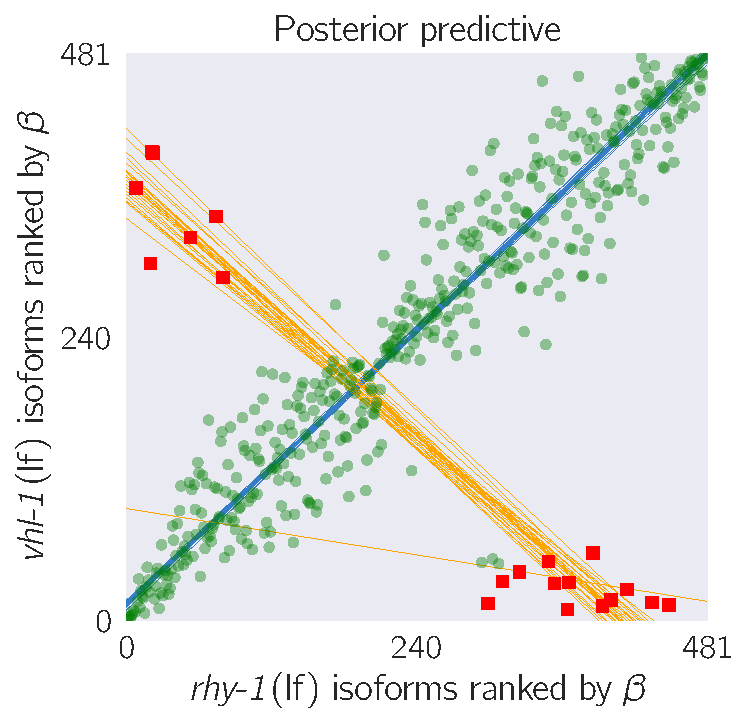
\includegraphics[width=.4\linewidth]{hypims/multiplemodes-ed.pdf}
\caption{
A feedback loop can generate transcriptomes that are both
correlated and anti-correlated. The \vhl{}/\rhy{} STP shows a cross-pattern.
Green large points are inliers to the first
regression. Red squares are outliers to the first regression. Only the red
small points were used for the secondary regression. Blue lines are representative
samples of the primary bootstrapped regression lines. Orange lines are
representative samples of the secondary bootstrapped regression lines.
}
\label{fig:xpattern}
\end{figure}



If the above is correct, then it should be possible to identify
\gene{egl-9}-independent, \rhy{}-dependent target genes in a
logically consistent way.
One erroneous way to identify these targets is via
subtractive logic. Using subtractive logic, we would identify genes that are
differentially expressed in \rhy{} mutants but not in \egl{} mutants.  Such a
gene set would
consist of almost 700 genes. One major drawback of subtractive logic is that it
cannot be applied when feedback loops exist between the genes in question.
Another problem is that the set of identified genes are statistically indistinguishable
from false positive and false negative hits because they have no distinguishing
property beyond the condition that they should be differentially expressed in
one mutant but not the other. In fact, this is exactly the behavior expected of
false-positive or false-negative hits---presence in one, but not multiple, mutants.
We need to consider the relationship between two genes before we can begin to
identify targets which expression is dependent on one gene and independent
of the other.

\gene{rhy-1} and \gene{egl-9} share a well-defined relationship. \rhyp{}
inhibits \cyslp{},
which in turn inhibits \eglp{}~\citep{Ma2012}. Therefore, loss of \rhyp{} leads
to inactivation of \eglp{}, which leads to increase in the cellular levels of
\hifp{}. \hifp{} in turn causes the mRNA levels of \gene{rhy-1} and \gene{egl-9}
to increase,
as they are involved in the \gene{hif-1}-dependent hypoxia response. However, since
\gene{rhy-1} has been mutated, the observed transcriptome is
\rhyp{} `null'; \eglp{} `null'; \hifp{} `on'. The situation is similar for
\egl{}, except that \rhyp{}
is not inactive, and therefore the observed transcriptome is the result of
\rhyp{} `up'; \eglp{} `null'; and \hifp{} `on'. From this pattern, we conclude that
the \egl{} and \rhy{} transcriptomes should exhibit a cross-pattern when plotted
against each other: The positive
arm of the cross is the result of the \eglp{} `null'; \hifp{} `on' dynamics; and the
negative arm reflects the different direction of \rhyp{} activity between
transcriptomes. No negative arm is visible (with the exception of two
outliers, which are annotated as pseudogenes in WormBase). Therefore, in this
dataset we do not find genes that have \gene{egl-9} independent,
\gene{rhy-1}-dependent expression patterns.

We also identified a main hypoxia response induced by disinhibiting
\gene{hif-1} (355 genes) by identifying genes that were commonly up-regulated
amongst \egl{}, \rhy{} and \vhl{} mutants. Although the hypoxic response is likely
to involve between three and seven times more genes (assuming the \rhy{} transcriptome
reflects the maximal hypoxic response), this is a conservative
estimate that minimizes false positive results, since these changes were
identified in four different genotypes with three replicates each. This response
included five transcription factors (\gene{W02D7.6}, \nhr{}, \gene{ztf-18},
\gene{nhr-135} and \gene{dmd-9}). The full list of genes associated with the
hypoxia response can be found in the Supplementary Table 1.
% TODO: SI numbering

\gene{hif-1}-independent effects of \gene{egl-9} have been reported
previously~\citep{Park2012}, which led us to question whether we could identify
similar effects in our dataset. We have observed that \hif{} displays a modest
increase in the transcription of \gene{rhy-1}, from which we speculated that
\eglp{} would have increased activity in the \hif{} mutant compared to the wild-type.
Therefore, we searched for genes that were regulated in an opposite manner between
\hif{} and \eglhif{}, and that were regulated in the same direction between
all \egl{} genotypes. We did not find any genes that met these conditions.

We also searched for genes with \gene{hif-1} independent, \gene{vhl-1}-dependent gene
expression and found \vhltargets{} genes, which can be found in the Supplementary
Table 2.
Finally, we searched for candidates directly regulated by \gene{hif-1}. Initially, we
searched for genes that had were significantly altered in \hif{} genotypes in one
direction, but altered in the opposite direction in mutants that activate the
\hifp{} response. Only two genes (\emph{R08E5.3}, and \emph{nit-1}) met these
conditions. This could reflect the fact that \hifp{} exists at very low
levels in \cel{}, so loss of function mutations in \gene{hif-1} might only have
mild effects on its transcriptional targets. We reasoned that genes
that are overexpressed in mutants that induce the \hifp{} response would be enriched
for genes that are direct candidates.  We found \hiftargets{}  genes which have
consistently increased expression in mutants with a constitutive hypoxic response.
These genes can be found in the Supplementary Table 3.


\subsubsection*{Enrichment analysis of the hypoxia response}
\label{sub:ea_hypoxia}
To validate that our transcriptomes were correct, and to understand how
functionalities may vary between them, we subjected each decoupled response to
enrichment analysis using the WormBase Enrichment Suite~\citep{Angeles-Albores2016,
Angeles-Albores2016b}.

\begin{figure}[tbhp]
\centering
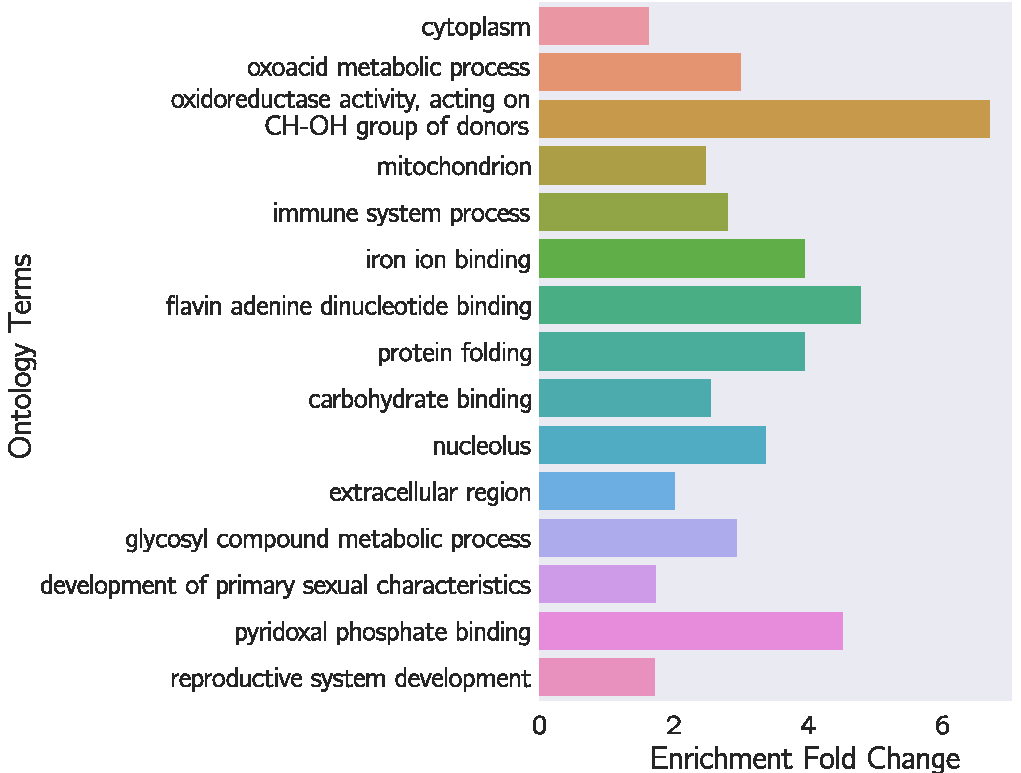
\includegraphics[width=.7\linewidth]{hypims/hypoxia_response_gea.pdf}
\caption{
Gene ontology enrichment analysis of genes associated with the main hypoxia response.
A number of terms reflecting catabolism and bioenergetics are enriched.
}
\label{fig:hyp_gea}
\end{figure}

We used gene ontology enrichment analysis (GEA) on the main hypoxia response program.
This showed that the terms `oxoacid metabolic process' (\qval{4}, 3.0 fold-change,
24 genes), `iron ion binding' (\qval{2}, 3.8 fold-change, 10 genes), and `immune
system process' (\qval{3}, 2.9 fold-change, 20 genes) were significantly enriched.
GEA also showed enrichment of the term `mitochondrion' (\qval{3}, 2.5 fold-change,
29 genes) (see Fig.~\ref{fig:hyp_gea}). Indeed, \hif{} has been implicated in
all of these biological and molecular functions~\citep{Luhachack2012,Ackerman2012,
Romney2011,Semenza2011}.
As benchmark on the quality of our data, we selected a set of 22 genes known to
be responsive to \hifp{} levels from the literature and asked whether these genes
were present in our hypoxia response list. We found $8/22$ known genes, which
constitutes a statistically significant result ($p<10^{10}$). The small number of
reporters found in this list probably reflects the conservative nature of our
estimates.
We studied the \gene{hif-1}-independent, \gene{vhl-1}-dependent gene set
using enrichment analysis but no terms were significantly enriched.

\subsection*{Identification of non-classical epistatic interactions}
\label{sub:hifoh}
\hif{} has traditionally been viewed as existing in a genetic OFF state under
normoxic conditions. However, our dataset indicates that \hifn{} genes show
altered expression when \gene{hif-1} function is removed in normoxic conditions.
Moreover, we observed positive correlations between \hif{} $\beta$ coefficients
and \egl{}, \vhl{} and \rhy{} $\beta$ coefficients in spite of the negative
regulatory relationships between these genes and \gene{hif-1}. Such
positive correlations could indicate a different relationship between these genes
than has previously been reported, so we attempted to substantiate them through
epistasis analyses.

To perform epistasis analyses, we first identified genes that exhibited violations
of the canonical genetic model of the hypoxia pathway. To this end, we searched for
genes that exhibited different behaviors between \egl{} and \vhl{}, or
between \rhy{} and \vhl{} (we assume that all results from the
\rhy{} transcriptome reflect a complete loss of \gene{egl-9} activity). We found
\hifohtargets{} that satisfied this condition (see Fig.~\ref{fig:hif1oh},
Supplemental Table 4).
Additionally, many of these genes exhibited a new kind of epistasis. Namely,
\gene{egl-9} was epistatic over \gene{vhl-1}. Identification of a set of genes
that have a consistent set of relationships between themselves suggests that
we have identified a new aspect of the hypoxia pathway.

\begin{figure}[tbhp]
\centering
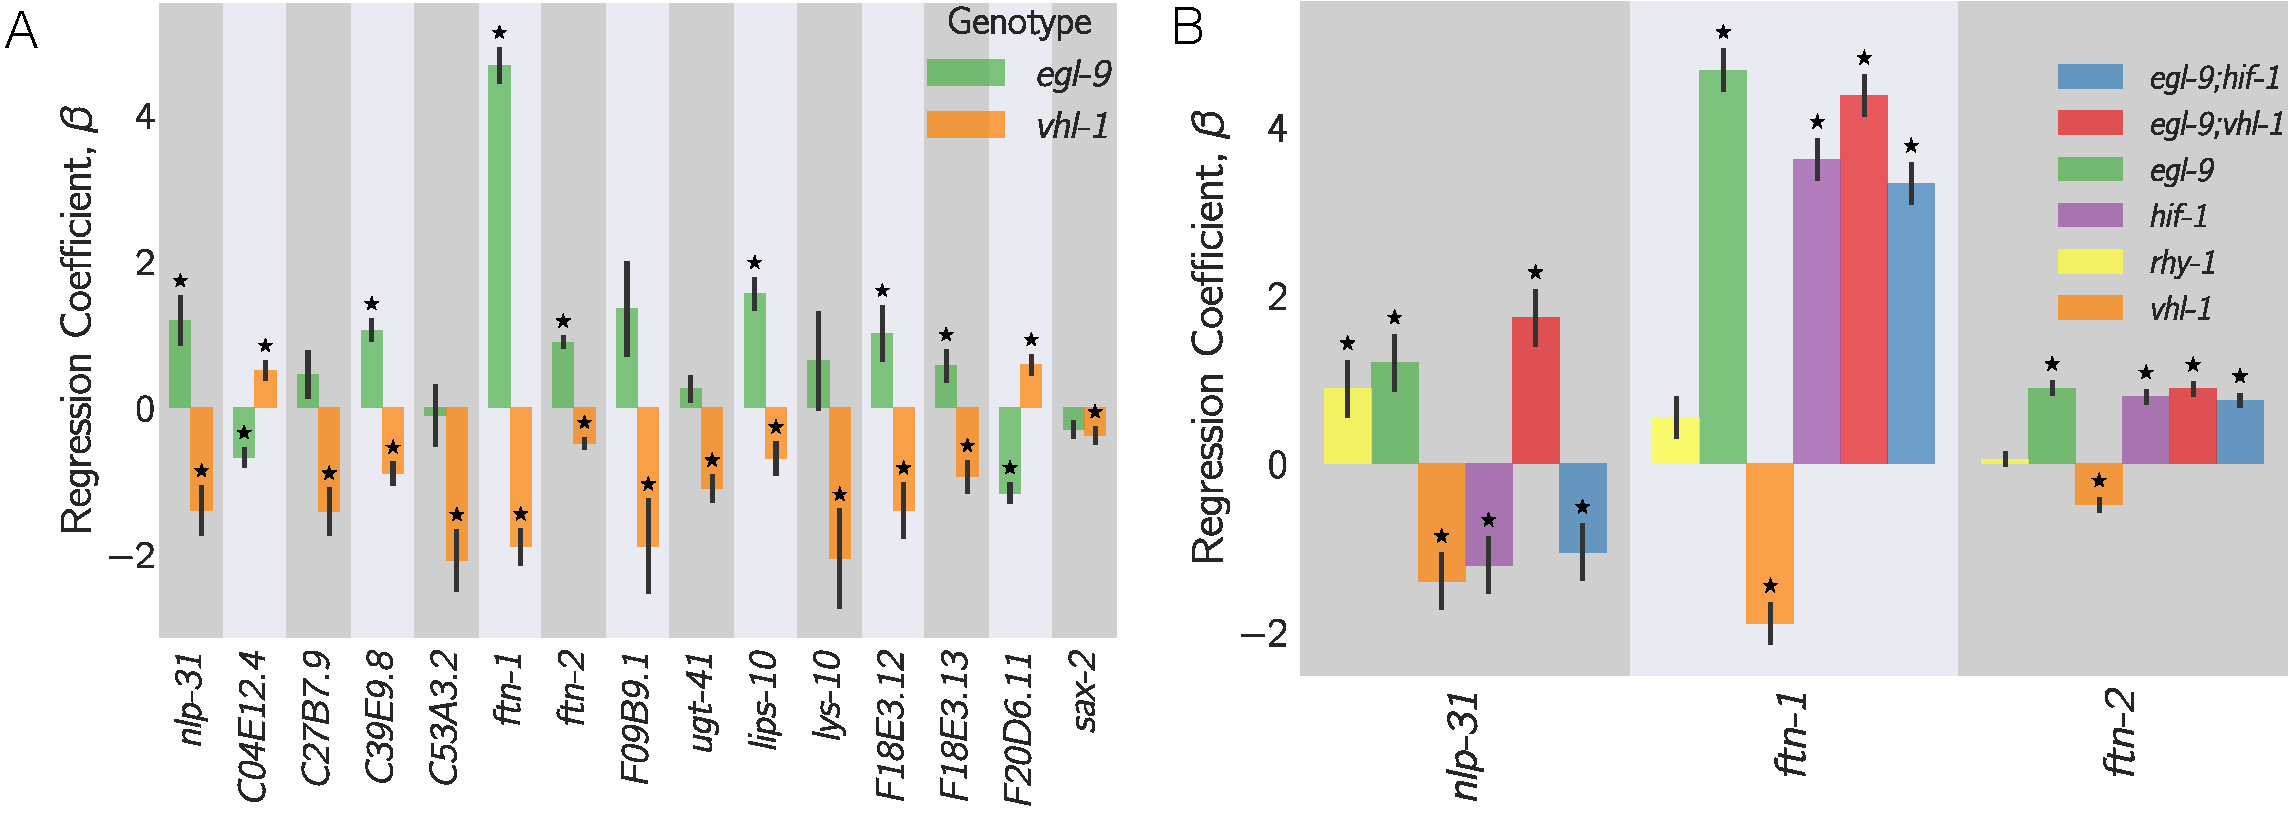
\includegraphics[width=\linewidth]{hypims/hif1oh-epistasis-horizontal.pdf}
\caption{
\textbf{A}. 27 genes in \cel{} exhibit non-classical epistasis in the hypoxia
pathway, characterized by opposite effects on gene expression, relative to the
wild-type, of of the \vhl{} compared to \egl{} (or
\rhy{}) mutants. Shown are a random selection of 15 the 27 genes for illustrative
purposes.
\textbf{B}. Representative genes showing that non-canonical epistasis shows a
consistent pattern. \vhl{} mutants have an opposite effect to \egl{}, but
\gene{egl-9} remains epistatic to \gene{vhl-1} and loss-of-function mutations in
\gene{hif-1} suppress the \egl{} phenotype. Asterisks show $\beta$ values
significantly different from 0 relative to wild-type (\qval{1}).
}
\label{fig:hif1oh}
\end{figure}

To illustrate this, we focused on three genes, \nlp{}, \ftna{} and \ftnb{}, which
epistasis patterns that we felt reflected the population well. \ftna{} and \ftnb{}
are both described in the literature as genes that are responsive to mutations in
the hypoxia pathway. Moreover, these genes have been previously described to have
aberrant behaviors~\citep{Ackerman2012,Romney2011}, specifically the
opposite effects of \egl{} and \vhl{}. These studies showed that loss of \vhl{}
decreases expression of \ftna{} and \ftnb{} using both RNAi and alleles, which
allays concerns of strain-specific interference. Moreover, Ackerman and Gems (2012)
showed that \gene{vhl-1} is epistatic to \gene{hif-1} for the \ftna{}
expression phenotype, and that loss of
\hifp{} is associated with increased expression of \ftna{} and \ftnb{}. We observed
that \gene{hif-1} was epistatic to \gene{egl-9}, and that \gene{egl-9} and
\gene{hif-1} both promoted \ftna{} and \ftnb{} expression.

Epistasis analysis of \ftna{} and \ftnb{} expression reveals that \gene{egl-9} is
epistatic to \gene{hif-1}; that \gene{vhl-1} has opposite effects to \gene{egl-9},
and that \gene{vhl-1} is epistatic to \gene{egl-9}. Analysis of \nlp{}
reveals similar relationships. \nlp{} expression is decreased in \hif{},
and increased in \egl{}. However, \gene{egl-9} is epistatic to \gene{hif-1}.
Like \ftna{} and \ftnb{}, \gene{vhl-1} has the opposite effect to \gene{egl-9},
yet is epistatic to \gene{egl-9}. We propose in the Discussion a model for how
\hifp{} might regulate these targets.

\subsection*{\hifp{} in the cellular context}
\label{sub:metabolism}

We identified the transcriptional changes
associated with bioenergetic pathways in \cel{} by extracting from
WormBase all genes associated with the tricarboxylic acid (TCA) cycle, the
electron transport chain (ETC) and with the \cel{} GO term energy reserve.
Previous research has described the effects of mitochondrial dysfunction in
eliciting the hypoxia response~\citep{Lee2010}, but transcriptional feedback
from \hifp{} into bioenergetic pathways has not been as extensively in \cel{},
as in vertebrates (see, for example~\citep{Semenza1994,Semenza2012}).
We also searched for the changes in ribosomal components and the proteasome, as
well as for terms relating to immune response (see Fig~\ref{fig:genomewide}).

\begin{figure}[tbhp]
\centering
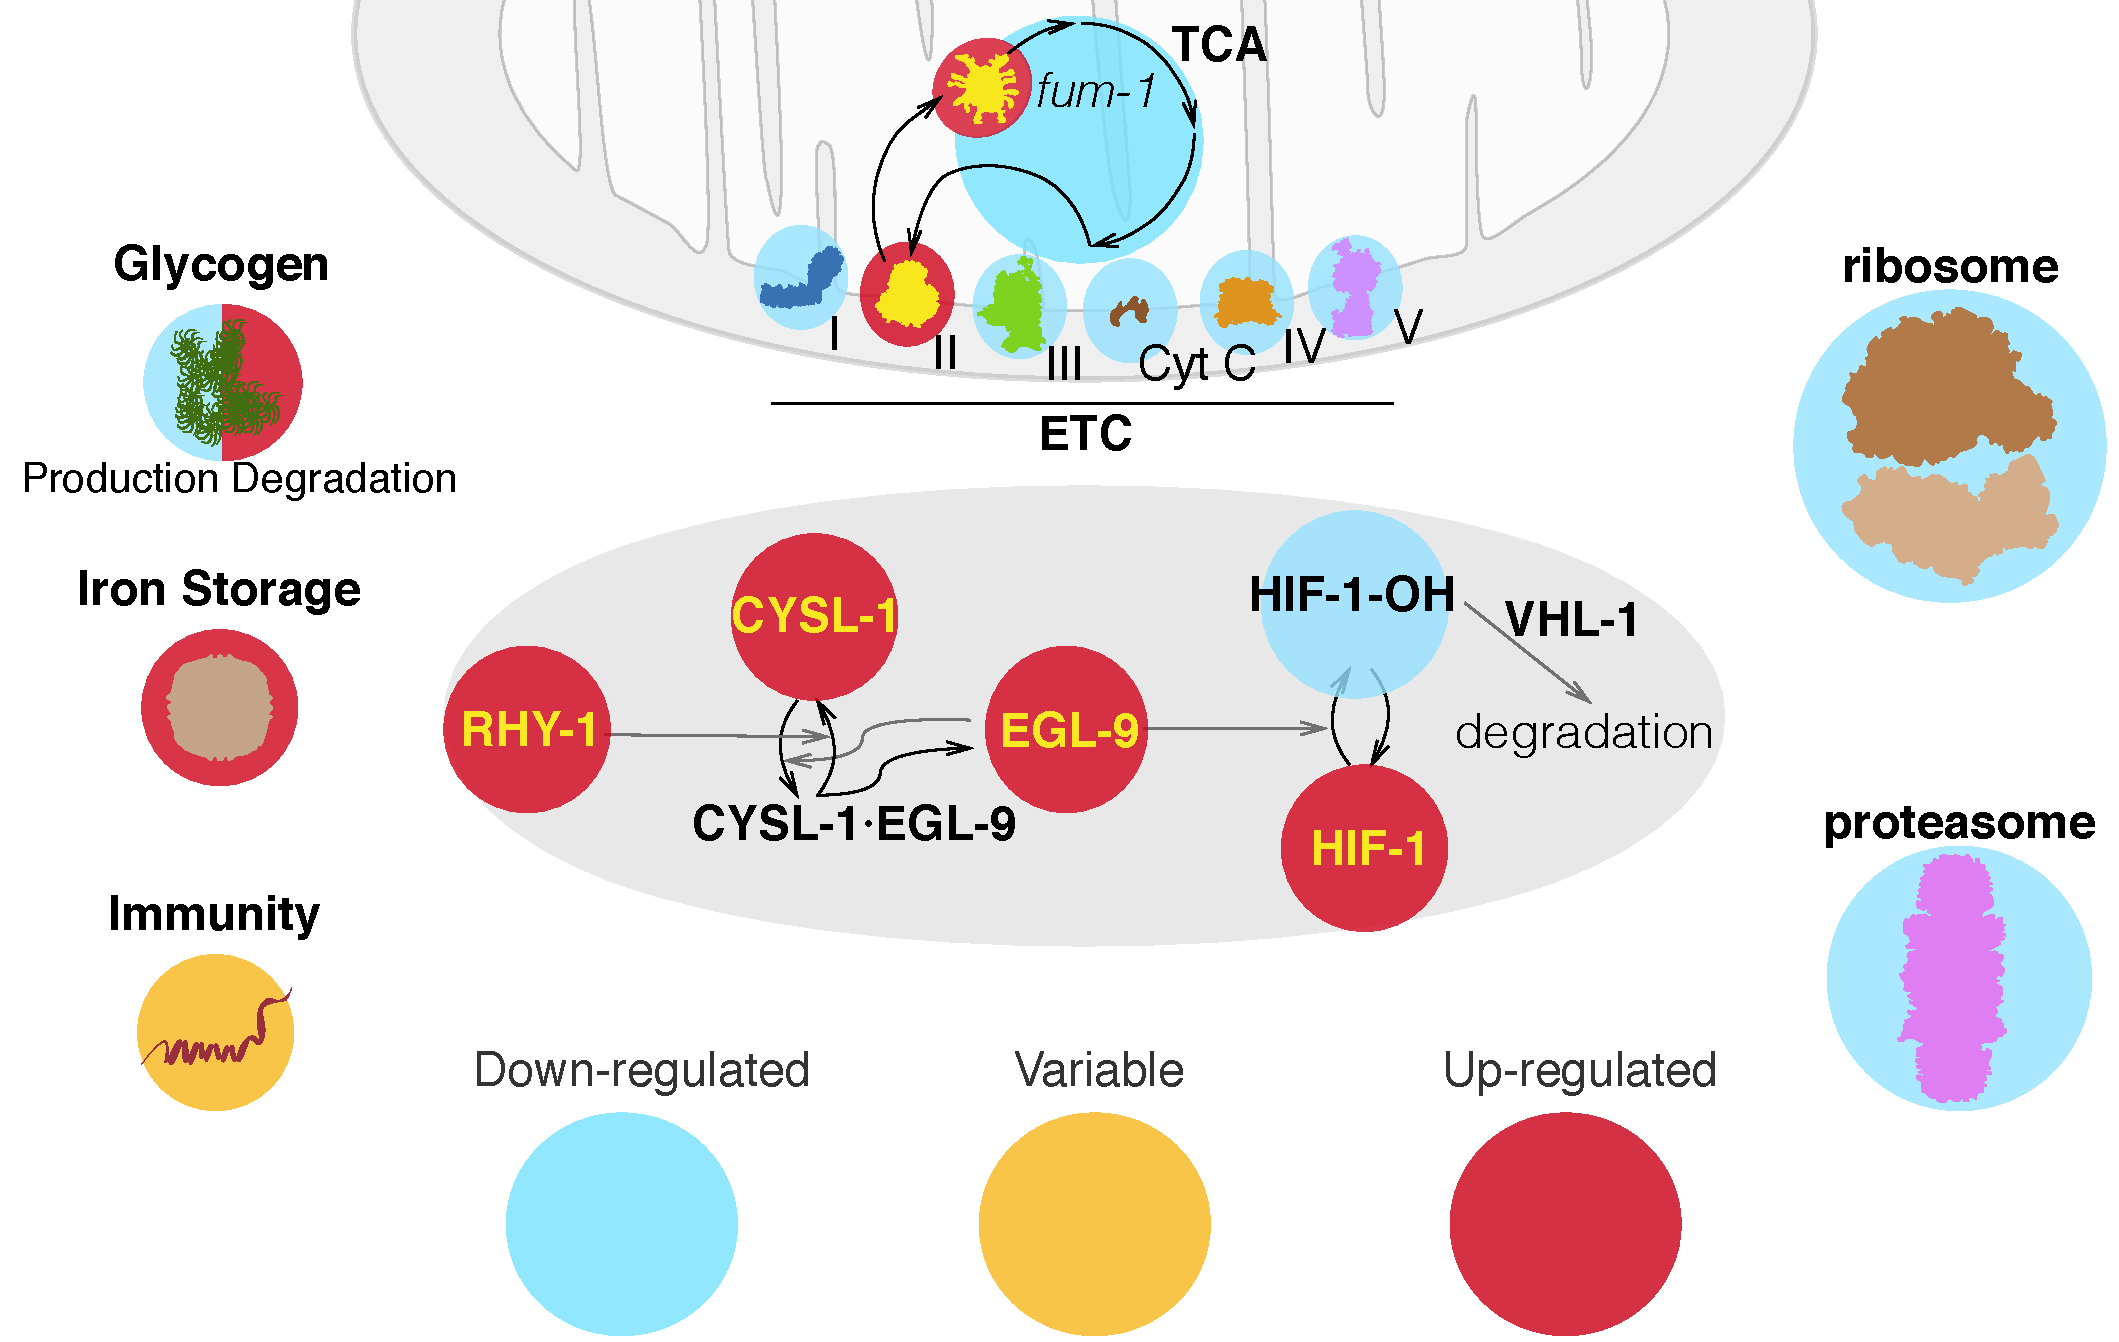
\includegraphics[width=.7\linewidth]{hypims/hif1genomewide.pdf}
\caption{
A graphic summary of the genome-wide effects of \hifp{} from our RNA-seq data.
}
\label{fig:genomewide}
\end{figure}

\subsubsection*{Bioenergetic pathways}
Our data shows that most of the enzymes involved in the TCA cycle and in the ETC
are down-regulated when \hifp{} is induced in agreement with the previous
literature~\citep{Semenza2012}.
However, the fumarase gene \gene{fum-1} and the mitochondrial complex II stood out
as notable exceptions to the trend, as they were up-regulated in every single
genotype that causes deployment of the hypoxia response. FUM-1 catalyzes the
reaction of fumarate into malate, and complex II catalyzes the reaction of
succinate into fumarate. Complex II has been identified as a source of reserve
respiratory capacity in neonatal rat cardiomyocytes previously~\citep{Pfleger2015}.
We found two energy reserve genes that were down-regulated by \hifp{}.
\gene{aagr-1} and \gene{aagr-2}, which are predicted to function in glycogen
catabolism~\citep{Sikora2010}.
Three distinct genes involved in energy reserve were up-regulated. These genes were
\gene{ogt-1}, which encodes O-linked GlcNac Transferase gene; \gene{T04A8.7},
encoding an ortholog of human glucosidase, acid beta (GBA); and \gene{T22F3.3},
encoding ortholog of human glycogen phosphorylase isozyme in the muscle (PYGM).

\subsubsection*{Protein synthesis and degradation}
\hif{} is also known to inhibit protein synthesis and translation in varied
ways.~\citep{Brugarolas2004}. Most reported effects of
\hifp{} on the translation machinery are posttranslational, and no reports to date
show transcriptional control of the ribosomal machinery in \cel{} by \hifp{}. We
used the WormBase Enrichment Suite Gene Ontology
dictionary~\citep{Angeles-Albores2016b} to extract 143 protein-coding genes
annotated as `structural constituents of the ribosome' and we queried whether
they were differentially expressed in our mutants. \egl{}, \vhl{}, \rhy{} and
\egl{};\vhl{} showed differential expression of 91 distinct ribosomal constituents
(not all constituents were detected in all genotypes). For every one of these
genotypes, these genes were always down-regulated. In contrast, \hif{} showed
up-regulation of a single ribosomal constituent.

Next, we asked whether \hifp{} has any transcriptional effects on the
proteasomal constituents; no such effects of \hifp{} on the proteasome
have been reported in \cel{}. Out of 40 WormBase-annotated proteasomal constituents,
we found 31 constituents that were differentially expressed in at least one of the
four genotypes that induce a hypoxic response. Every gene we found was down-regulated
in at least two out of the four genotypes we studied.

\section*{Discussion}
\subsection*{The \cel{} hypoxia pathway can be reconstructed entirely from
             RNA-seq data}
In this paper, we have shown that whole-organism transcriptomic phenotypes
can be used to reconstruct genetic pathways and to discern previously overlooked
or uncharacterized genetic interactions. We successfully reconstructed the hypoxia
pathway, and inferred order of action (\gene{rhy-1} activates \gene{egl-9},
\gene{egl-9} and \gene{vhl-1} inhibit \gene{hif-1}), and we were able to infer
from transcriptome-wide epistasis measurements that \gene{egl-9} exerts
\gene{vhl-1}-dependent and independent inhibition on \gene{hif-1}.

\subsection*{\hifp{} and the cellular environment}

In addition to reconstructing the pathway, our dataset allowed us
to observe a wide variety of physiologic changes that occur as a result of the
\hifp{}-dependent hypoxia response. In particular, we observed down-regulation of most
components of the TCA cycle and the mitochondrial electron transport chain with
the exceptions of \gene{fum-1} and the mitochondrial complex II.\@ The mitochondrial
complex II catalyzes the reaction of succinate into fumarate.
In mouse embryonic fibroblasts, fumarate has been
shown to antagonize \hifp{} prolyl hydroxylase domain (PHD) enzymes, which are
orthologs of \eglp{}~\citep{Sudarshan2009}.
If the inhibitory role of fumarate on PHD enzymes is conserved in \cel{},
upregulation of complex II by \hifp{} during hypoxia may increase
intracellular levels of fumarate, which in turn could lead to artificially high
levels of \hifp{}
even after normoxia resumes. The increase in fumarate produced by the complex
could be compensated by increasing expression of \gene{fum-1}. Increased fumarate
degradation allows \cel{} to maintain plasticity in the hypoxia pathway, keeping
the pathway sensitive to oxygen levels.

\subsection*{Interpretation of the non-classical epistasis in the hypoxia pathway}
The observation of almost 30 genes that exhibit a specific pattern of non-classical
epistasis suggests the existence of previously undescribed aspects of the hypoxia
pathway. Some of these non-classical epistases had been observed
previously~\citep{Ackerman2012,Romney2011,Luhachack2012}, but
no satisfactory mechanism has been proposed to explain this biology.
\citet{Romney2011} and \citet{Ackerman2012}
suggest that \hifp{} integrates information on iron concentration in the
cell to bind to the \ftna{} promoter, but could not definitively establish
a mechanism.
It is unclear why deletion of \gene{hif-1} induces \ftna{}
expression, deletion of \gene{egl-9} also causes induction of \ftna{} expression,
but deletion of \gene{vhl-1} removes this inhibition. Moreover, \citet{Luhachack2012}
have previously reported that certain genes important for the \cel{} immune response
against pathogens reflect similar expression patterns. Their interpretation
was that \gene{swan-1}, which encodes a binding partner to \eglp{}~\citep{Shao2010},
is important for modulating \hifp{} activity in some manner. The lack of a
conclusive double mutant analysis in this work means the role of SWAN-1 in
modulation of \hifp{} activity remains to be demonstrated. Nevertheless, mechanisms
that call for additional transcriptional modulators become less likely given the
number of genes with different biological functions that exhibit the same pattern.

\begin{figure}[tbhp]
\centering
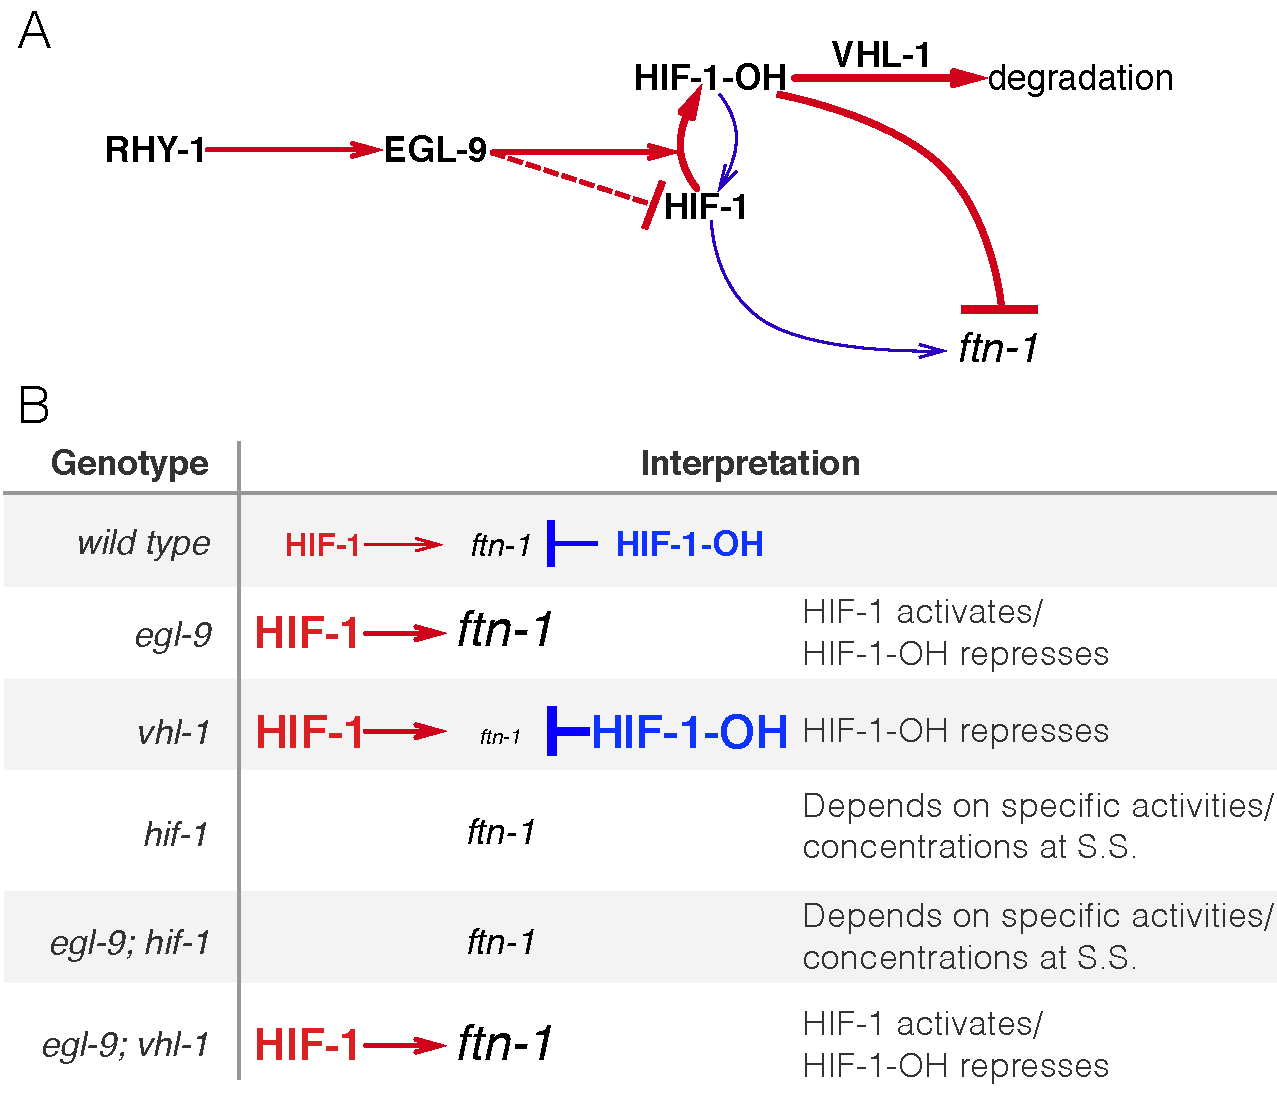
\includegraphics[width=.5\linewidth]{hypims/hif1oh_model.pdf}
\caption{
A hypothetical model showing a mechanism where \hifp{}-hydroxyl antagonises
\hifp{}.
\textbf{A}. Diagram showing that RHY-1 activates EGL-9.
EGL-9 hydroxylates HIF-1 in an oxygen dependent fashion. Under normoxia, HIF-1
is rapidly hydroxylated and only slowly does hydroxylated HIF-1 return to its
original state. EGL-9 can also inhibit HIF-1 in an oxygen-independent fashion.
HIF-1 hydroxyl is rapidly degraded in a VHL-1 dependent fashion. In our model,
HIF-1 and HIF-1 hydroxyl have opposing effects on transcription. The width of the
arrows represents the rates under normoxic conditions.
\textbf{B}. Table showing the effects of loss-of-function mutations on HIF-1 and
HIF-1 hydroxyl activity, showing how this can potentially explain the behavior
of \gene{ftn-1} in each case.  S.S = Steady-state.
}
\label{fig:hif1oh_table}
\end{figure}

One way to resolve this problem without invoking additional genes is to
consider \hifp{} as a protein with both activating and inhibiting states. In fact,
\hifp{} already exists in two states in \cel{}: unmodified \hifp{} and
\hifp{}-hydroxyl (\hifp{}-OH). Under this model, \hifp{}-hydroxyl antagonizes
the effects of \hifp{} for certain genes like \ftna{} or \nlp{}. Loss of
\gene{vhl-1} stabilizes \hifp{}-hydroxyl.
A subset of genes that are sensitive to \hifp{}-hydroxyl will be inhibited as a
result of the increase in the amount of this species, in spite of loss of
\gene{vhl-1} function also increasing the level of non-hydroxylated \hifp{}.
On the other hand, \egl{} selectively removes all \hifp{}-hydroxyl, stimulating
accumulation of \hifp{} and promoting gene activity. Whether deletion of \hif{}
is overall activating or inhibiting will depend on the relative activity of each
protein state under normoxia (see Fig.~\ref{fig:hif1oh_table}).

Multiple lines of circumstantial evidence that \hifp{}-hydroxyl plays a role
in the functionality of the hypoxia pathway. First, \hifp{}-hydroxyl is
challenging to study genetically because no mimetic mutations are available with
which to study the pure hydroxylated \hifp{} species. Second, although mutations in
the Von-Hippel Landau gene stabilize the hydroxyl species, they also increase the
quantity of non-hydroxylated \hifp{} by mass action.
Finally, since \hifp{} is detected low levels
in cells under normoxic conditions~\citep{Wang1993}, total \hifp{} protein
(unmodified \hifp{} plus \hifp{}-hydroxyl) is often tacitly assumed to be
vanishingly rare and therefore biologically inactive.

Our data show hundreds of genes that change expression in response
to loss of \gene{hif-1} under normoxic conditions. This establishes that there is
sufficient total \hifp{} protein to be biologically active.
Our analyses also revealed that \hif{} shares
positive correlations with \egl{}, \rhy{} and \vhl{}, and that each of these genotypes
also shows a secondary negative rank-ordered expression correlation with each other.
These cross-patterns between all loss of function of inhibitors of \hifp{} and
\hif{} can be most easily explained if \hifp{}-hydroxyl is biologically active.

A homeostatic argument can be made in favor of the activity of \hifp{}-hydroxyl.
At any point in time, the cell must measure the levels of
multiple metabolites at once. The \gene{hif-1}-dependent hypoxia
response integrates information from O$_2$, $\alpha$-ketoglutarate
(2-oxoglutarate) and iron concentrations in the cell. One way to
integrate this information is by encoding it only in the effective hydroxylation
rate of \hifp{} by \eglp{}. Then the dynamics in this system will evolve
exclusively as a result of the total amount of \hifp{} in the cell. Such a system
can be sensitive to fluctuations in the absolute concentration of
\hifp{}~\citep{Goentoro2009a}. Since the absolute levels of \hifp{} are low in
normoxic conditions, small fluctuations in protein copy-number represent can
represent a large fold-change in \hifp{} levels. These fluctuations would
not be problematic for genes that must be turned on only under conditions of severe
hypoxia---presumably, these genes would be associated with low affinity
sites for \hifp{}, so that they are only activated when \hifp{} levels are far
above random fluctuations.

For yet other sets of genes that must change expression in response to the hypoxia
pathway, it may not make as much sense to integrate metabolite information
exclusively via \eglp{}-dependent hydroxylation of \hifp{}. In particular, genes
that may function to increase survival in mild hypoxia may benefit from regulatory
mechanisms that can sense minor changes in environmental conditions and which
therefore benefit from robustness to transient changes in protein copy number.
Likewise, genes that are involved in iron or $\alpha$-ketoglutarate metabolism
(such as \ftna{}) may benefit from being able to sense, accurately, small and
consistent deviations from basal concentrations of these metabolites. For these
genes, the information may be better encoded by using \hifp{} and
\hifp{}-hydroxyl as an activator/repressor pair. Such circuits are
known to possess distinct advantages for controlling output in a manner that
is robust to transient fluctuations in the levels of their
components~\citep{Hart2012,Hart2013}.

Our RNA-seq data suggests that one of these atypical targets of \hifp{}
may be \rhyp{}. Although \gene{rhy-1} does not exhibit non-classical
epistasis, \hif{} and \eglhif{} both had increased expression levels of \gene{rhy-1}.
We speculate that if \gene{rhy-1} is controlled by both \hifp{} and \hifp{}-hydroxyl,
then this might imply that \hifp{} regulates the expression of its pathway (and
therefore itself) in a manner that is robust to total \hifp{} levels.

\subsection*{Insights into genetic interactions from vectorial phenotypes}

Here, we have described a set of straightforward methods that can be in theory
applied to any vectorial phenotype. Genome-wide methods afford a lot of information,
but genome-wide interpretation of the results is often extremely challenging.
Each method has its own advantages and disadvantages. We briefly discuss these
methods, their uses and their drawbacks.

Principal component analysis
is computationally tractable and clusters can often be visually detected with
ease. However, PCA can be misleading, especially when the dimensions represented
do not explain a very large fraction of the variance present in the data. In addition,
principal dimensions are the product of a linear combination of vectors, and therefore
must be interpreted with extreme care. In this case, the first principal dimension
separated genotypes that increase \hifp{} protein levels from those that decrease
it, but this dimension is a mix of vectors of change in gene expression. Although
PCA showed that there is information hidden in these genotypes, it was not enough
by itself to provide biological insight.

Whereas PCA operates on all genotypes simultaneously, correlation analysis is a
pairwise procedure that measures how predictable the gene
expression changes are in a mutant given the vector of expression changes in
another. Like PCA, correlation analysis is easy and fast to perform. Unlike PCA,
the product of a correlation analysis is a single number with a straightforward
interpretation. However, correlation analysis is particularly sensitive to outliers.
Although a common strategy is to rank-transform expression data to mitigate
outliers, rank-transformations do not remove the cross-patterns that appear when
feedback loops or other complex interactions are present between two genes.
Such cross-patterns can still lead to vanishing correlations if both patterns are
equally strong. Therefore, correlation analyses must take into account the possible
existence of systematic outliers. Moreover, correlation values must be measured
for both interactions in cross-patterned rank plots. Weighted correlations could
be informative for ordering genes along pathways.
A drawback of correlation
analysis is that the number of pairwise comparisons that must be made increases
combinatorially, though strategies could be used to decrease the total number of
effective comparisons.

Epistasis plots are a novel way to visualize epistasis in vectorial phenotypes.
Here, we have shown how an epistasis plot can be used to identify interactions
between two single mutants and a double mutant. In reality, epistasis plots
can be generated for any set of measurements involving a set of $N$ mutants and
an $N$-mutant genotype. Epistasis plots can accumulate an arbitrary number of
points within them, possess a rich structure that can be visualized and have
straightforward interpretations for special slope values.

Another way to analyze epistasis is via general linear models (GLMs) that include
interaction terms between two or more genes. In this way, GLMs can quantify
the epistatic effect of an interaction on single genes. We and
others~\citep{Dixit2016,Angeles-Albores2016a} have previously used GLMs to identify
gene sets that are epistatically regulated by two or more inputs. While powerful,
GLMs suffer from the multiple comparison problem. Correcting for false positives
using well-known multiple comparison corrections such as FDR~\citep{Storey2003}
tends to increase false negative rates.  Moreover, since GLMs attempt to estimate
effect magnitudes for individual gene or isoform expression levels, they
effectively treat each gene as an independent quantity, which prevents better
estimation of the magnitude and direction of the epistasis between two genes.

Epistasis plots do not suffer from the multiple comparison problem because the
number of tests performed is orders of magnitudes smaller than the number
of tests performed by GLMs. Ideally, in an epistasis plot we need only perform
3 tests---rejection of additive, unbranched and suppressive null models---compared
with the tens of thousands of tests that are performed in GLMs. Moreover, the
magnitude of epistasis between two genes can be estimated using hundreds of genes,
which greatly improves the statistical resolution of the epistatic coefficient.
This increased resolution is important because the size and magnitude of the
epistasis has specific consequences for the type of pathway that is expected.

Any quantitative use of genome-wide datasets requires a good experimental setup.
Here, we have demonstrated that whole-organism RNA-seq can be used to dissect
molecular pathways in exquisite detail when paired with experimental designs that
are motivated by classical genetics. Much more research will be necessary
to understand whether epistasis has different consequences in the microscopic
realm of transcriptional phenotypes than in the macroscopic world that geneticists
have explored previously. Our hope is that these tools, coupled with the classic
genetics experimental  designs, will reveal hitherto unknown aspects of genetics
theory.

\section*{Methods}
\label{sec:methods}
\subsection*{Nematode strains and culture}
Strains used were N2 wild-type Bristol,
CB5602 \gene{vhl-1}(\emph{ok161}),
CB6088 \gene{egl-9}(\emph{sa307})~\gene{hif-1}(\emph{ia4}),
CB6116 \gene{egl-9}(\emph{sa307});\gene{vhl-1}(\emph{ok161}),
JT307 \gene{egl-9}(\emph{sa307}),
ZG31 \gene{hif-1}(\emph{ia4}),
RB1297 \gene{rhy-1}(\emph{ok1402}).
All lines were grown on standard
nematode growth media (NGM) plates seeded with OP50 \ecol{} at 20\degree{}C
(Brenner 1974).

\subsection*{RNA Isolation}
Unsynchronized lines were grown on NGM plates at 20C and eggs harvested by
sodium hypochlorite treatment. Eggs were plated on 6 to 9 6cm NGM plates
with ample OP50 \ecol{} to avoid starvation and grown at
20\degree{}C.  Worms were staged and harvested based on the time after plating,
vulva morphology and the absence of eggs.  Approximately 30--50 non-gravid young
adults were picked and placed in 100$\mu$L of TE pH 8.0 at 4\degree{}C in
$0.2$mL PCR tubes.   After settling and a brief spin in microcentrifuge
approximately $80\mu$L of TE (Ambion AM 9849) was removed from the top of the
sample and individual replicates
were snap frozen in liquid N2. These replicate samples were then digested with
Proteinase K (Roche Lot No. 03115 838001 Recombinant Proteinase K PCR Grade) for
15min at 60\degree{} in the presence of 1\% SDS and 1.25$\mu$L
RNA Secure (Ambion AM 7005). RNA samples were then taken up in 5 Volumes of
Trizol (Tri Reagent Zymo Research) and processed and treated with DNase I using
Zymo MicroPrep RNA Kit (Zymo Research Quick-RNA MicroPrep R1050).
RNA was eluted in RNase-free water and divided into aliquots and stored at
-80\degree{}C. One aliquot of each replicate was analyzed using a NanoDrop (Thermo
Fisher) for impurities, Qubit for concentration and then analyzed on an Agilent
2100 BioAnalyzer (Agilent Technologies).
Replicates were selected that had RNA integrity numbers (RIN) equal or greater
than 9.0 and showed no evidence of bacterial ribosomal bands, except for the
ZG31 mutant where one of three replicates had a RIN of 8.3.

\subsection*{Library Preparation and Sequencing}
10ng of quality checked total RNA from each sample was
reverse-transcribed into cDNA using the Clontech SMARTer Ultra Low Input RNA for
Sequencing v3 kit (catalog \#634848) in the SMARTSeq2 protocol
~\citep{Picelli2014}.  RNA was denatured at 70$\degree{}$C for 3 minutes
in the presence of dNTPs, oligo dT primer and spiked-in quantitation standards
(NIST/ERCC from Ambion, catalog \#4456740).  After chilling to 4$\degree{}$C, the
first-strand reaction was assembled using the LNA TSO primer described in
\citet{Picelli2014}, and run at 42$\degree{}$C for 90 minutes, followed by
denaturation at 70$\degree{}$C for 10 minutes.  The entire first strand reaction
was then used as template for 13 cycles of PCR using the Clontech v3 kit.
Reactions were cleaned up with 1.8X volume of Ampure XP SPRI beads (catalog
\#A63880) according to the manufacturer’s protocol.  After quantification using
the Qubit High Sensitivity DNA assay, a 3ng aliquot of the amplified cDNA was
run on the Agilent HS DNA chip to confirm the length distribution of the
amplified fragments.  The median value for the average cDNA lengths from all
length distributions was 1076bp.  Tagmentation of the full length cDNA for
sequencing was performed using the Illumina/Nextera DNA library prep kit (catalog
\#FC-121--1030).  Following Qubit quantitation and Agilent BioAnalyzer profiling,
the tagmented libraries were sequenced. Libraries were sequenced on Illumina
HiSeq2500 in single read mode with the read length of 50nt to an average depth
of 15 million reads per sample following manufacturer's instructions. Base calls
were performed with RTA 1.13.48.0 followed by conversion to FASTQ with bcl2fastq
1.8.4. Spearman correlation of the transcripts per million (TPM) for each
genotype showed that every pairwise correlation within genotype was $>0.9$.

\subsection*{Read Alignment and Differential Expression Analysis}
We used Kallisto to perform read pseudo-alignment and performed differential
analysis using Sleuth. We fit a general linear model for a transcript $t$ in
sample $i$:

\begin{equation}
  y_{t,i} = \beta_{t, 0} + \beta_{t, genotype}\cdot{}X_{t, i} +
  \beta_{t, batch}\cdot{}Y_{t, i} + \epsilon_{t, i}
\end{equation}

where $y_{t, i}$ are the logarithm transformed counts; $\beta_{t, genotype}$ and
$\beta_{t, batch}$ are parameters of the model, and which can be interpreted as
biased estimators of the log-fold change; $X_{t, i}, Y_{t, i}$ are indicator
variables describing the conditions of the sample; and $\epsilon_{t, i}$ is the
noise associated with a particular measurement.

\subsection*{Genetic Analysis, Overview}
Genetic analysis of the processed data was performed in Python 3.5. Our scripts
made extensive use of the Pandas, Matplotlib, Scipy, Seaborn, Sklearn, Networkx,
Bokeh, PyMC3, and TEA libraries~\citep{Team2014,McKinney2011,Oliphant2007,
Pedregosa2012,Salvatier2015,VanDerWalt2011,Hunter2007,Angeles-Albores2016,Waskom}.
Our analysis is available in a Jupyter Notebook~\citep{Perez2007}. All code and
required data (except the raw reads) are available at
\url{https://github.com/WormLabCaltech/mprsq} along with version-control
information. Our Jupyter Notebook and interactive graphs for this project can be
found at \url{https://wormlabcaltech.github.io/mprsq/}. Raw reads were deposited
in the Short Read Archive under the study accession number SRP100886.


\subsection*{Weighted Correlations}
Pairwise correlations between transcriptomes where calculated by first identifying
the set of differentially expressed genes (DEGs) common to both transcriptomes under
analysis. DEGs were then rank-ordered according to their regression coefficient,
$\beta$.\ Bayesian robust regressions were performed using a Student-T distribution.
Bayesian analysis was performed using the PyMC3 library~\citep{Salvatier2015}
(\texttt{pm.glm.families.StudenT} in Python). If the correlation has an average
value $>1$, the correlation coefficient was set to 1.

Weights were calculated as the proportion of genes that were $<1.5$ standard
deviations away from the primary regression out of the entire set of shared DEGs
for each transcriptome.

\subsection*{Epistasis Analysis}
For a double mutant $X^-Y^-$, we used the single mutants $X^-$ and $Y^-$ to
find expected value of the coefficient for a double mutant under an additive model
for each isoform $i$.
Specifically,
\begin{equation}
  \beta_{\mathrm{Add},i} = \beta_{X,i} + \beta_{Y,i}.
\end{equation}

Next, we find the difference, $\Delta_i$, between the observed double mutant
expression coefficient, $\beta_{XY, \mathrm{Obs},i}$, and the predicted
expression coefficient under an additive model for each isoform $i$.

To calculate the transcriptome-wide epistasis coefficient, we plotted
($\beta_{\mathrm{Add},i}, \Delta_i$) and found the line of best fit using
orthogonal distance regression using the \texttt{scipy.odr} package in Python.
We performed
non-parametric bootstrap sampling of the ordered tuples with replacement using
5,000 iterations to generate a probability distribution of slopes of best fit.

There are as many models as epistatic relationships. For quantitative phenotypes,
epistatic relationships (except synthetic interactions) can be generally
expressed as:

\begin{equation}
  \beta_{XY} = \sum_{g\in G} \lambda_g \beta_g,
  \label{eq:epi}
\end{equation}

where $P_i$ is the quantitative phenotype belonging to the genotype $i$; $G$ is
the set of single mutants $\{X, Y\}$ that make up the double mutant, $XY$; and
$\lambda_g$ is the contribution of the phenotype $P_g$ to $P_{XY}$.
Additive interactions between genes are the result of setting $\lambda_g=1$. All
other relationships correspond to setting  $\lambda_X=0,~\lambda_Y=1$ or
$\lambda_X=1,~\lambda_Y=0$.

A given epistatic interaction can be simulated by predicting the double mutant
phenotype under that interaction and re-calculating the y-coordinates. The
recalculated y-coordinates can then be used to predict the possible epistasis
coefficients for the cases where $X$ is epistatic over $Y$, and $Y$ is epistatic
over $X$.

To select between theoretical models, we implemented an approximate Bayesian
Odds Ratio. We defined a free-fit model, $M_1$, that found the line of best fit
for the data:

\begin{equation}
  P(\alpha~|M_1, D) \propto \prod_{(x_i, y_i, \sigma_i)\in D}
  \exp{\frac{
            (y_i - \alpha\cdot x_i)^2
            } % numerator
            {
            2\sigma_i
            } % denominator
            } \cdot (1+\alpha^2)^{-3/2},
  \label{eq:free_model}
\end{equation}

where $\alpha$ is the slope of the model to be determined, $x_i, y_i$ were the
x- and y-coordinates of each point respectively, and $\sigma_i$ was the standard
error associated with the y-value. We minimized the
negative logarithm of equation~\ref{eq:free_model} to obtain the most likely
slope given the data, $D$ (\texttt{scipy.optimize.minimize} in Python). Finally,
we approximated the odds ratio as:

\begin{equation}
  OR = \frac{
  P(D~|\alpha^*, M_1)\cdot (2\pi)^{1/2}\sigma_{\alpha^*} % numerator
  }{P(D~| M_i)}, % denominator
\end{equation}

where $\alpha^*$ is the slope found after minimization, $\sigma_\alpha^*$ is the
standard deviation of the parameter at the point $\alpha^*$ and $P(D~|M_i)$ is the
probability of the data given the parameter-free model, $M_i$.

\subsection*{Enrichment Analysis}
Tissue, Phenotype and Gene Ontology Enrichment Analysis were carried out using
the WormBase Enrichment Suite for Python~\citep{Angeles-Albores2016b,
Angeles-Albores2016}.



\subsubsection*{Author Contributions:}
This work was supported by HHMI with whom PWS is an investigator
and by the Millard and Muriel Jacobs Genetics and Genomics Laboratory at
California Institute of Technology.
All strains were provided by the CGC, which is funded by NIH Office of Research
Infrastructure Programs (P40 OD010440).
This article was written with support of the Howard Hughes Medical Institute.
This article wouldn't be possible without help from Dr.\_ Igor Antoshechkin who
performed all sequencing.
We thank Hillel Schwartz for all of his careful advice.
We would like to thank Jonathan Liu, Han Wang, and Porfirio Quintero for helpful
discussion.

  \printbibliography[heading=subbibliography]
\end{refsection}

\chapter{Transcriptomic description of an endogenous female state in \cel{}}
\begin{refsection}
  % new commands
\newcommand{\fog}{\emph{\mbox{fog-2(lf)}}}

% gene numbers
\newcommand{\fogn}{1,881}
\newcommand{\agen}{5,592}
\newcommand{\interactionn}{1,318}
\newcommand{\coexpressed}{905}
\newcommand{\intersectn}{1,040}
\newcommand{\femalen}{405}

% tf numbers
\newcommand{\tfaging}{145}
\newcommand{\tffog}{60}
\newcommand{\tfinteraction}{36}

% number of genes in gold standard
\newcommand{\goldn}{1,056}
\newcommand{\goldfound}{506}
\newcommand{\goldpval}{$<10^{-38}$}

% website commands
\newcommand{\website}{
            \url{https://wormlabcaltech.github.io/Angeles_Leighton_2016/}
            }
\newcommand{\webref}{
\href{https://wormlabcaltech.github.io/Angeles_Leighton_2016/}{website}}


\section*{Abstract}
\textbf{
  Understanding genome and gene function in a whole organism requires us to
  fully comprehend the life cycle and the physiology of the organism in question.
  Although \cel{} is traditionally thought of as a hermaphrodite, XX animals exhaust
  their sperm and become endogenous females after 3 days of egg-laying.
  The molecular physiology of this state has not been as intensely studied as other
  parts of the life cycle, despite documented changes in behavior and metabolism
  that occur at this stage. To study the female state of \cel{}, we measured the
  transcriptomes of 1st day adult hermaphrodites; endogenous, 6th day adult females;
  and at the same time points, mutant \fog{} worms that have a feminized germline
  phenotype. At these time points, we could separate the effects of biological
  aging from the transition into the female state.\@ \fog{} mutants partially phenocopy
  6 day adult wild-type animals and exhibit fewer differentially expressed genes as
  they age throughout these 6 days. Therefore, \emph{fog-2} is epistatic to age as
  assessed by this transcriptomic phenotype, which indicates that both factors act
  on sperm status to mediate entry into the female state. These changes are enriched
  in transcription factors canonically associated with neuronal development and
  differentiation. Our data provide a high-quality picture of the changes that
  happen in global gene expression throughout the period of early aging in the
  worm.}
\vspace{10mm}


\section*{Introduction}

Transcriptome analysis by RNA-seq~\citep{Mortazavi2008} has allowed for indepth
analysis of gene expression changes between life stages and environmental
conditions in many species~\citep{Gerstein2014,Blaxter2012}.
\emph{Caenorhabditis~elegans}, a genetic model nematode with extremely
well defined and largely invariant development~\citep{Sulston1977,Sulston1983},
has been subjected to extensive transcriptomic analysis across all stages of
larval development~\citep{Hillier2009,Boeck2016,Murray2012}
and many stages of embryonic development~\citep{Boeck2016}. Although RNA-seq was
used to develop transcriptional profiles of the mammalian aging process soon
after its invention~\citep{Magalhaes2010}, few such studies have been conducted
in \cel{} past the entrance into adulthood.

A distinct challenge to the study of aging transcriptomes in \cel{} is the
hermaphroditic lifestyle of wild-type individuals of this species. Young adult
hermaphrodites are capable of self-fertilization~\citep{Brenner1974,Corsi2015},
and the resulting embryos will contribute RNA to whole-organism RNA extractions.
Most previous attempts to study the \cel{} aging transcriptome have addressed
the aging process only indirectly, or relied on the use of genetically or
chemically sterilized animals to avoid this problem~\citep{Murphy2003,
Halaschek-wiener2005,Lund2002,McCormick2012,Eckley2013,Boeck2016,Rangaraju2015}.
In addition, most of these studies obtained transcriptomes using microarrays,
which are less accurate than RNA-seq, especially for low-expressed
genes~\citep{Wang2014}.

Here, we investigate what we argue is a distinct state in the \cel{} life cycle,
the endogenous female state. Although \cel{} hermaphrodites emerge into adulthood
already replete with sperm, after about 3 days of egg-laying the animals become
sperm-depleted and can only reproduce by mating, This marks a transition into
what we define as the endogenous female state. This state is behaviorally
distinguished by increased male-mating success~\citep{Garcia2007}, which may be
due to an increased attractiveness to males~\citep{Morsci2011}. This increased
attractiveness acts at least partially through production of volatile chemical
cues~\citep{Leighton2014}.
These behavioral changes are also coincident with functional deterioration of
the germline~\citep{Andux2008}, muscle~\citep{Herndon2002},
intestine~\citep{McGee2011} and nervous system~\citep{Liu2013}, changes
traditionally attributed to the aging process~\citep{Golden2007}.

To decouple the effects of aging and sperm-loss, we devised a two factor
experiment. We examined wild-type XX animals at the beginning of
adulthood (before worms contained embryos, referred to as 1st day adults) and
after sperm depletion (6 days after the last molt, which we term 6th day
adults). Second, we examined feminized XX animals that fail to produce sperm but
are fully fertile if supplied sperm by mating with males (see
Fig.~\ref{fig:wormlife}). We used \fog{} mutants to obtain feminized animals.
\gene{fog-2} is involved in germ-cell sex determination in the hermaphrodite
worm and is required for sperm production~\citep{Schedl1988,Clifford2000}.

\cel{} defective in sperm formation will never transition into or out of a
hermaphroditic stage. As time moves forward, these spermless worms only exhibit
changes related to biological aging. We also reasoned that we might be able to
identify gene expression changes due to different life histories: whereas
hermaphrodites lay almost 300 eggs over three days, spermless females do not lay
a single one. The different life histories could affect gene expression.

Here, we show that we can detect a transcriptional signature associated both
with loss of hermaphroditic sperm and entrance into the endogenous female state.
We can also detect changes associated specifically with biological aging.
Loss of sperm leads to increases in the expression levels of transcription
factors that are canonically associated with development and cellular
differentiation and enriched in neuronal functions.
Biological aging causes transcriptomic changes consisting of \agen{} genes
in \cel{}. 4,552 of these changes occur in both genotypes we studied,
indicating they do not depend on life history or genotype. To facilitate
exploration of the data, we have generated a website where we have deposited
additional graphics, as well as all of the code used to generate these analyses:
\website{}.

% figure experiment design
\begin{figure}[htbp]
\renewcommand{\familydefault}{\sfdefault}\normalfont{}
\centering
% \captionsetup{width=0.5\linewidth}
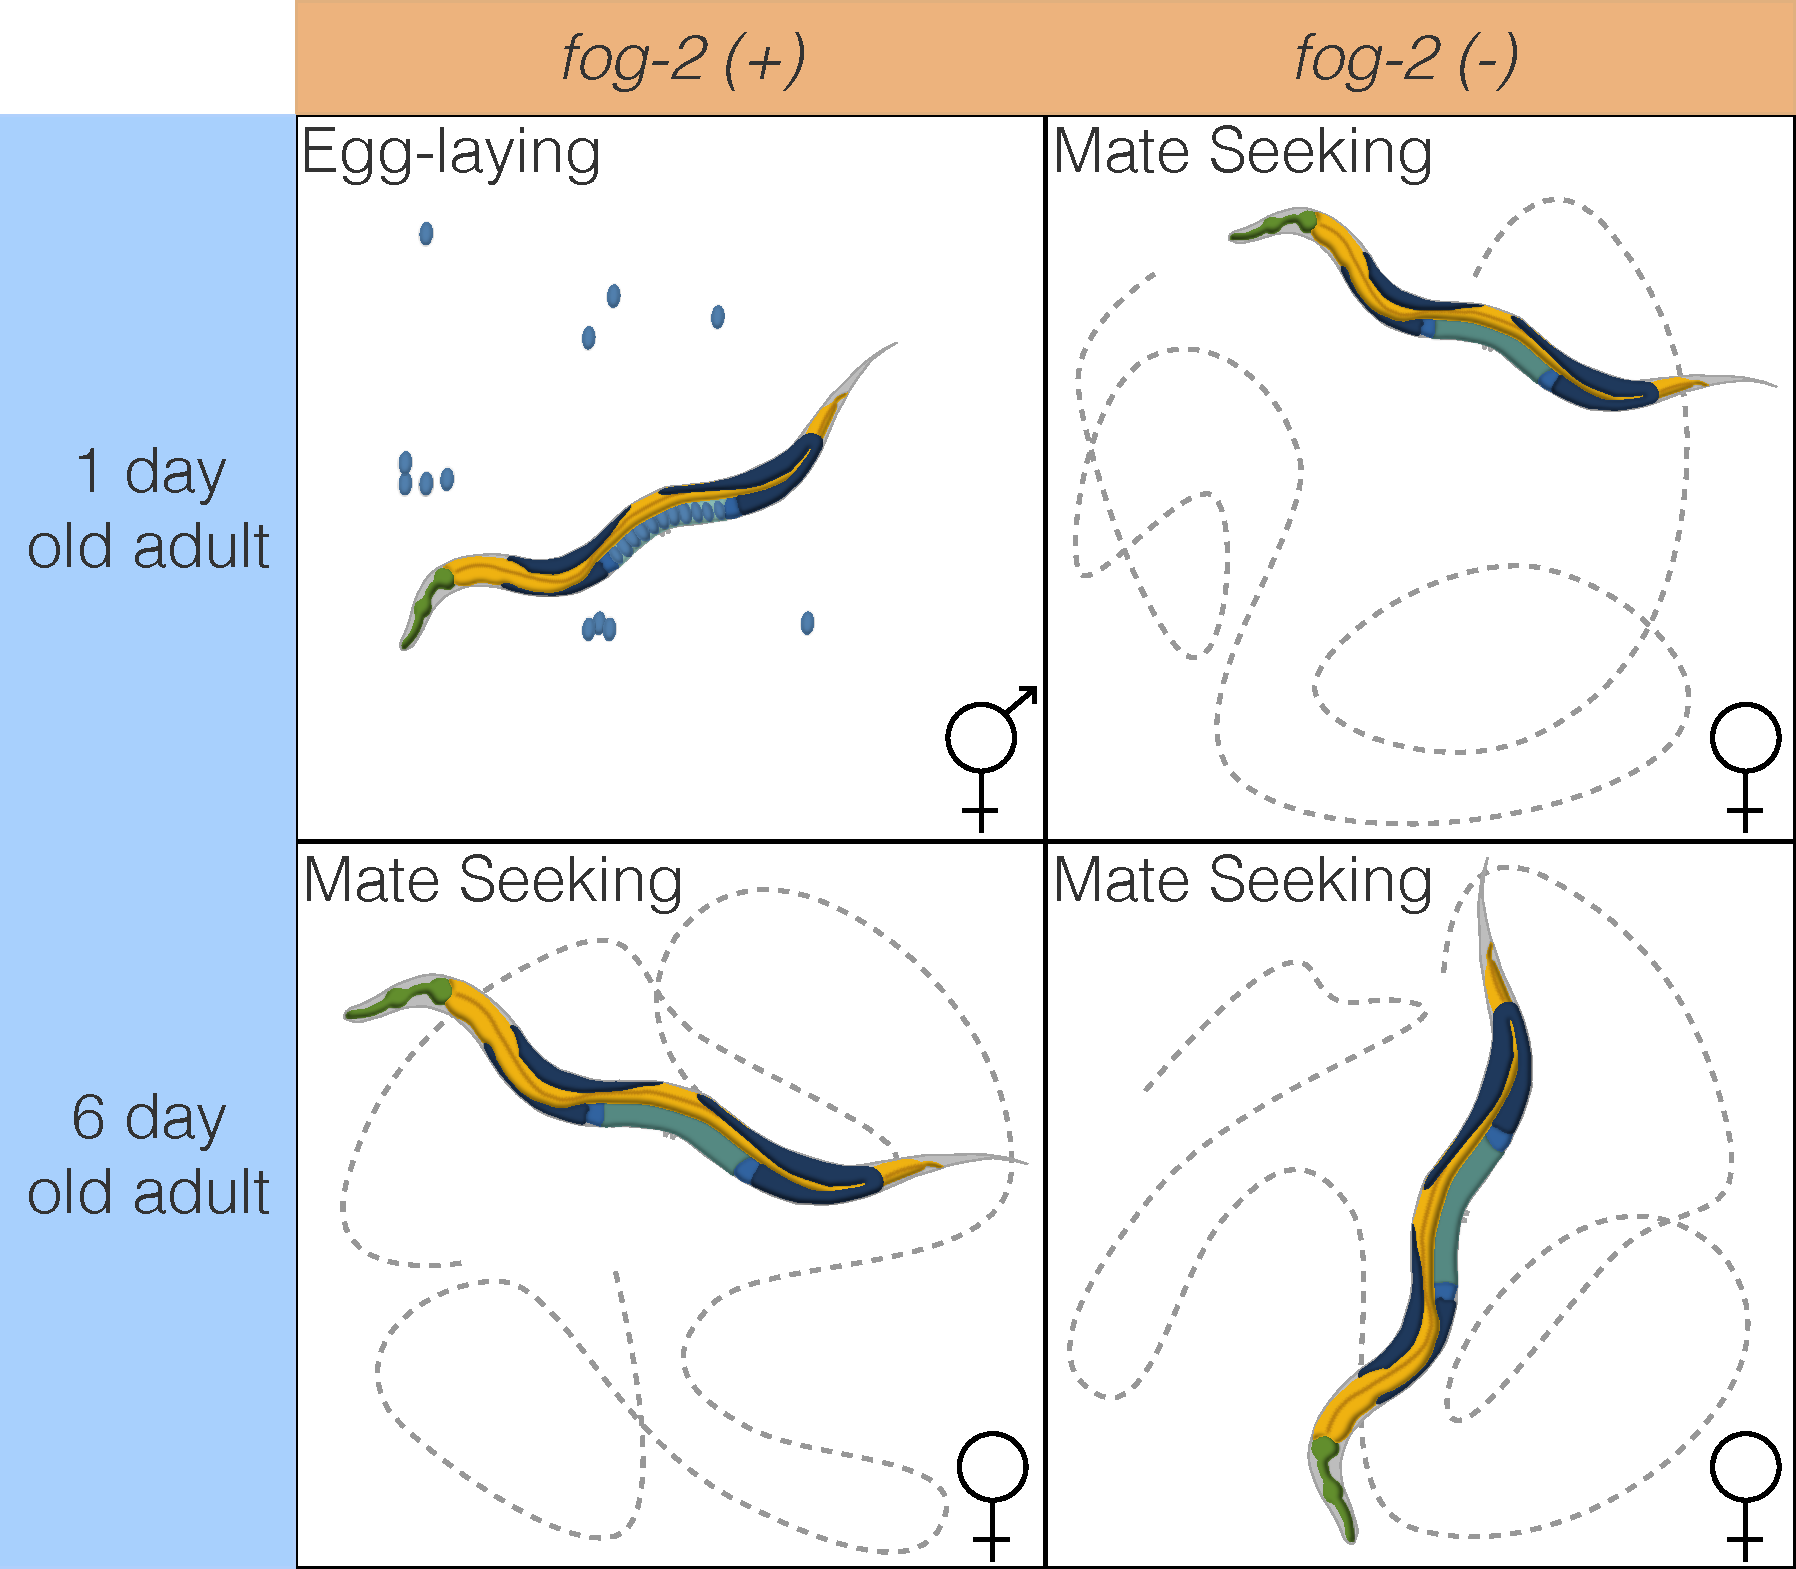
\includegraphics[width=0.5\linewidth]{femims/worm_life_fog2_vs_n2.pdf}
\caption{Experimental design to identify genes associated with sperm loss and
with aging. Studying the wild-type worm alone would measure time- and
sperm-related changes at the same time, without allowing us to separate these
changes. Studying the wild-type worm and a \fog{} mutant would enable us to
measure sperm-related changes but not time-related changes. By mixing both
designs, we can measure and separate both modules.
}%
\label{fig:wormlife}
\end{figure}


\section*{Materials and Methods}
\label{sec:materials_methods}

\subsection*{Strains}
\label{sub:Strains}
Strains were grown at 20\degree{}C on NGM plates containing \ecol{} OP50. We
used the laboratory \cel{} strain N2 as our wild-type strain~\citep{Brenner1974}.
We also used the N2 mutant strain JK574, which contains the \gene{fog-2(q71)}
allele, for our experiments.

\subsection*{RNA extraction}
\label{sb:rna_extraction}
Synchronized worms were grown to either young adulthood or the 6th day of
adulthood prior to RNA extraction. Synchronization and aging were carried out
according to protocols described previously~\citep{Leighton2014}. 1,000--5,000
worms from each replicate were rinsed into a microcentrifuge tube in S basal
(5.85g/L NaCl, 1g/L $\mathrm{K}_2\mathrm{HPO}_4$, 6g/L
$\mathrm{KH}_2\mathrm{PO}_4$), and then spun down at 14,000rpm for 30s. The
supernatant was removed and 1mL of TRIzol was added. Worms were lysed by
vortexing for 30~s at room temperature and then 20~min at 4\degree. The TRIzol
lysate was then spun down at 14,000rpm for 10~min at 4\degree{}C to allow
removal of insoluble materials. Thereafter the Ambion TRIzol protocol was
followed to finish the RNA extraction (MAN0001271 Rev. Date: 13 Dec 2012).
3 biological replicates were obtained for each genotype and each time point.

\subsection*{RNA-Seq}
\label{sb:rna_seq}
RNA integrity was assessed using RNA 6000 Pico Kit for Bioanalyzer (Agilent
Technologies \#5067--1513) and mRNA was isolated using NEBNext Poly(A) mRNA
Magnetic Isolation Module (New England Biolabs, NEB, \#E7490). RNA-Seq libraries
were constructed using NEBNext Ultra RNA Library Prep Kit for Illumina (NEB
\#E7530) following manufacturer’s instructions. Briefly, mRNA isolated from
$\sim1\mu$g of total RNA was fragmented to the average size of 200nt by
incubating at 94$\degree$C for 15~min in first strand buffer, cDNA was synthesized
using random primers and ProtoScript II Reverse Transcriptase followed by
second strand synthesis using Second Strand Synthesis Enzyme Mix (NEB).
Resulting DNA fragments were end-repaired, dA tailed and ligated to NEBNext
hairpin adaptors (NEB \#E7335).
After ligation, adaptors were converted to the ‘Y’ shape by treating with USER
enzyme and DNA fragments were size selected using Agencourt AMPure XP beads
(Beckman Coulter \#A63880) to generate fragment sizes between 250 and 350 bp.
Adaptor-ligated DNA was PCR amplified followed by AMPure XP bead clean up.
Libraries were quantified with Qubit dsDNA HS Kit (ThermoFisher Scientific
\#Q32854) and the size distribution was confirmed with High Sensitivity DNA Kit
for Bioanalyzer (Agilent Technologies \#5067--4626).
Libraries were sequenced on Illumina HiSeq2500 in single read mode with the read
length of 50nt following manufacturer's instructions. Base calls were performed
with RTA 1.13.48.0 followed by conversion to FASTQ with bcl2fastq 1.8.4.

\subsection*{Statistical Analysis}
\label{sb:statistics}

\subsubsection*{RNA-Seq Analysis}
RNA-Seq alignment was performed using Kallisto~\citep{Bray2016} with 200
bootstraps. The commands used for read-alignment are in the S.I. file 1.
Differential expression analysis was performed using Sleuth~\citep{Pimentel2016}.
The following General Linear Model (GLM) was fit:

\begin{align*}
  \log(y_i) =& \beta_{0,i} + \beta_{G,i}\dot~G + \\
  &\beta_{A,i}\dot~A + \beta_{A::G,i}\dot~A~G,
  \label{eqn:GLM}
\end{align*}

where $y_i$ are the TPM counts for the ith gene; $\beta_{0,i}$ is the intercept
for the ith gene, and $\beta_{X,i}$ is the regression coefficient for variable
$X$ for the $i$th gene; $A$ is a binary age variable indicating 1st day adult
(0) or 6th day adult (1) and $G$ is the genotype variable indicating wild-type
(0) or \fog{} (1); $\beta_{A::G, i}$ refers to the regression coefficient
accounting for the interaction between the age and genotype variables in the
$i$th gene. Genes were called significant if the FDR-adjusted q-value for any
regression coefficient was less than 0.1. Our script for differential analysis
is available on GitHub.

Regression coefficients and TPM counts were processed using Python 3.5 in a
Jupyter Notebook~\citep{Perez2007}. Data analysis was performed using the Pandas,
NumPy and SciPy libraries~\citep{McKinney2011,VanDerWalt2011,Oliphant2007}.
Graphics were created using the Matplotlib and Seaborn
libraries~\citep{Waskom,Hunter2007}. Interactive graphics were generated using
Bokeh~\citep{Team2014}.

Tissue, Phenotype and Gene Ontology Enrichment
Analyses (TEA, PEA and GEA, respectively) were performed using the WormBase
Enrichment Suite for Python~\citep{Angeles-Albores2016,Angeles-Albores106369}.

\subsection*{Data Availability}
\label{sb:data_availability}
Strains are available from the \emph{Caenorhabditis} Genetics Center. All of the
data and scripts pertinent for this project except the raw reads can be found on
our Github repository
\url{https://github.com/WormLabCaltech/Angeles_Leighton_2016}. File S1
contains the list of genes that were altered in aging regardless of genotype.
File S2 contains the list of genes and their associations with the \fog{}
phenotype. File S3 contains genes associated with the female state. Raw reads
were deposited to the Sequence Read Archive under the accession code SUB2457229.

\section*{Results and Discussion}
\begin{figure}[htbp]
\renewcommand{\familydefault}{\sfdefault}\normalfont{}
\centering
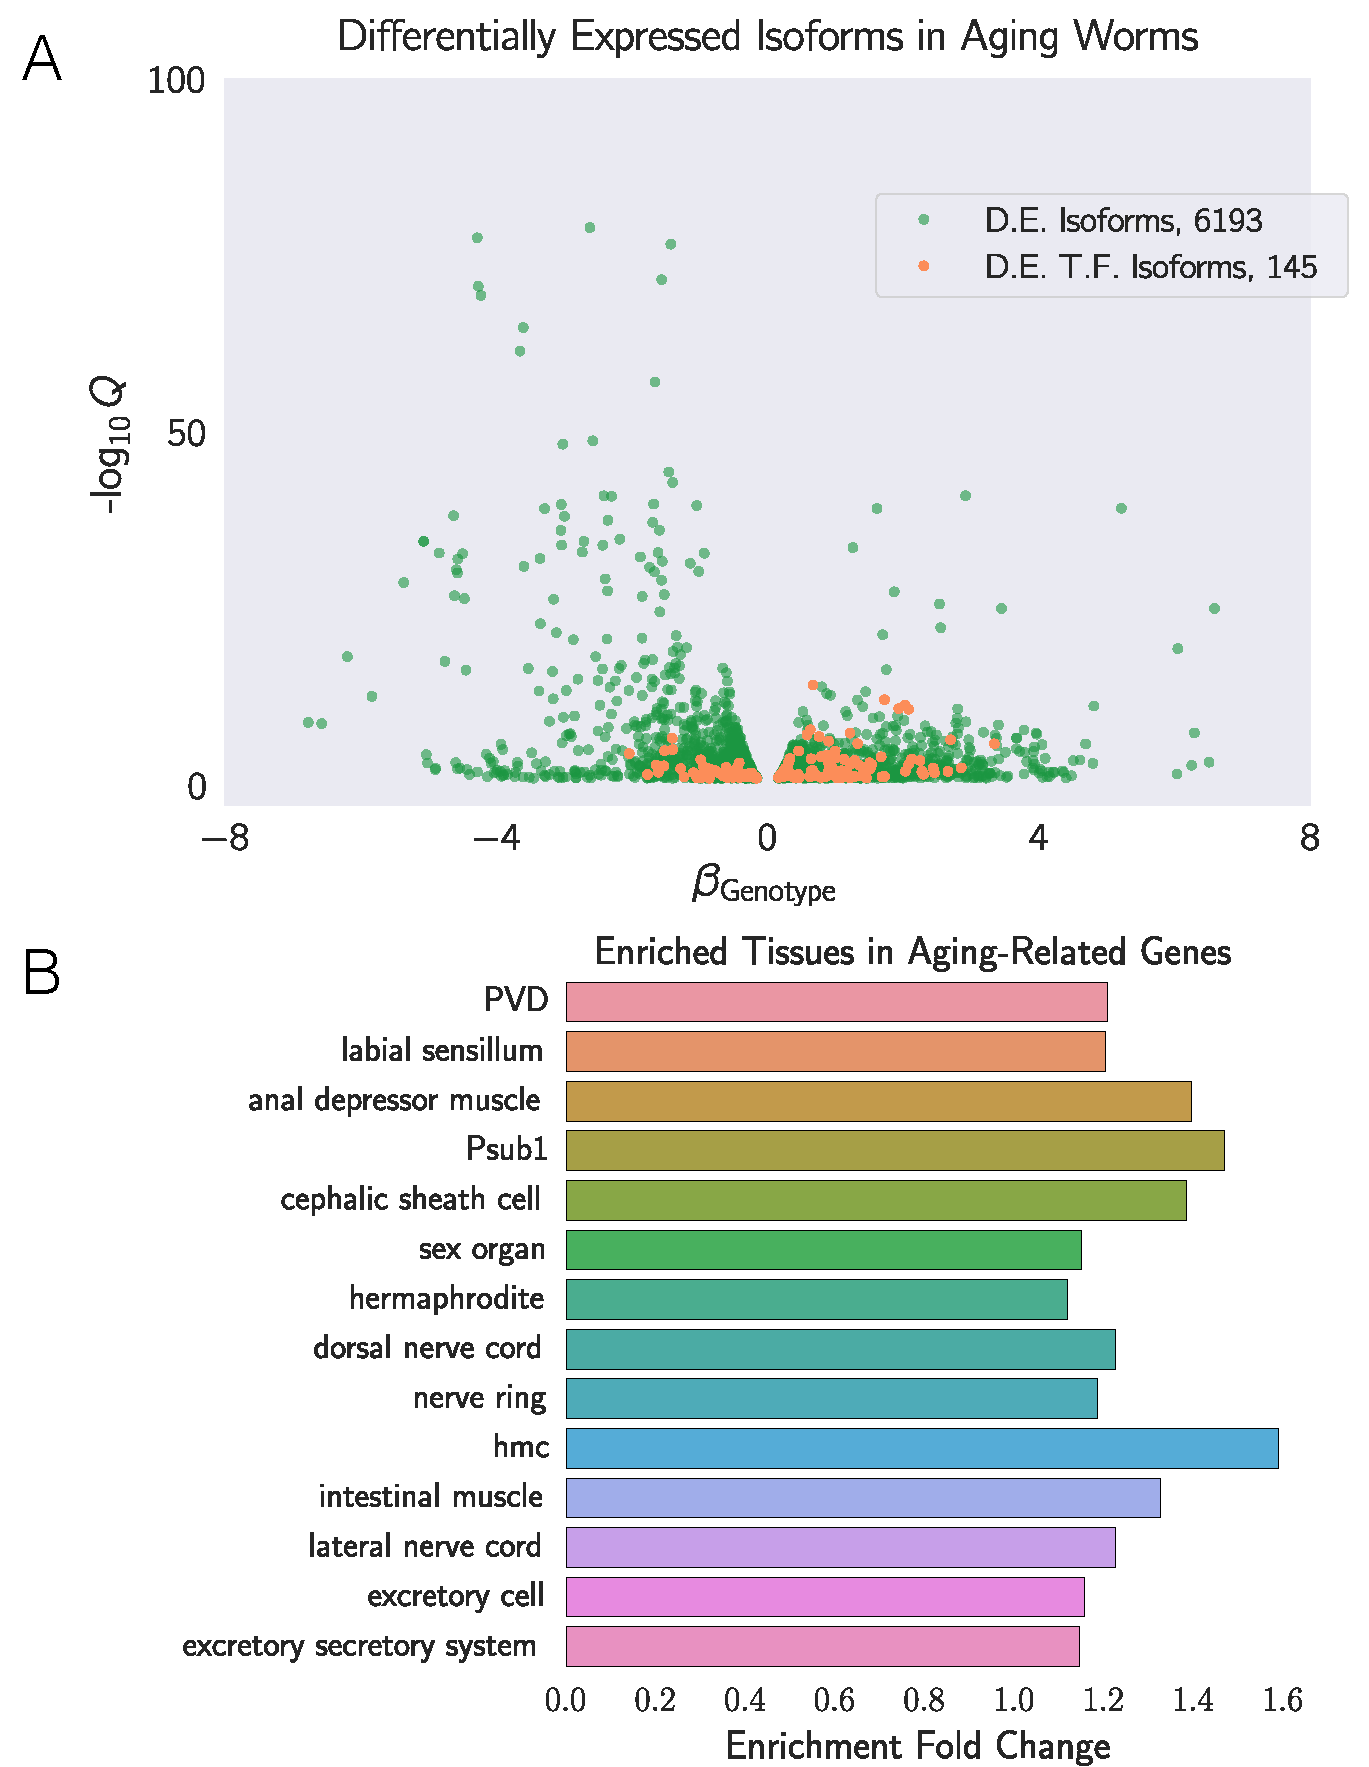
\includegraphics[width=.7\linewidth]{femims/aging_transcriptomics.pdf}
\caption{
\textbf{A} We identified a common aging transcriptome between N2 and
\fog{} animals, consisting of 6,193 differentially expressed isoforms totaling
\agen{} genes. The volcano plot is randomly down-sampled 30\% for ease of
viewing. Each point represents an individual isoform. $\beta{}_\mathrm{Aging}$
is the regression coefficient. Larger magnitudes of $\beta$ indicate a larger
log-fold change. The y-axis shows the negative logarithm of the q-values for
each point. Green points are differentially expressed isoforms; orange points
are differentially expressed isoforms of  predicted transcription factor
genes~\citep{Reece-Hoyes2005}. An interactive version of this graph can be found
on our \webref{}.
\textbf{B} Tissue Enrichment Analysis~\citep{Angeles-Albores2016} showed that
genes associated with muscle tissues and the nervous system are enriched in
aging-related genes. Only statistically significantly enriched tissues are shown.
Enrichment Fold Change is defined as $Observed/Expected$.\ hmc stands for head
mesodermal cell.
}
\label{fig:agingtranscriptome}
\end{figure}

\subsection*{Decoupling time-dependent effects from sperm-status via general
linear models}
\label{sub:Transcriptomics}
In order to decouple time-dependent effects from changes associated with loss
of hermaphroditic sperm, we measured wild-type and \fog{} adults at the 1st day
adult stage (before visible embryos were present) and 6th day adult stage, when
all wild-type hermaphrodites had laid all their eggs (see
Fig~\ref{fig:wormlife}), but mortality was still low
($<10\%$)~\citep{Stroustrup2013}.  We obtained 16--19 million reads mappable to
the \cel{} genome per biological replicate, which enabled us to identify
14,702 individual genes totalling 21,143 isoforms (see
Figure~\ref{fig:agingtranscriptome}a).

\begin{figure}[htbp]
\renewcommand{\familydefault}{\sfdefault}\normalfont{}
\centering
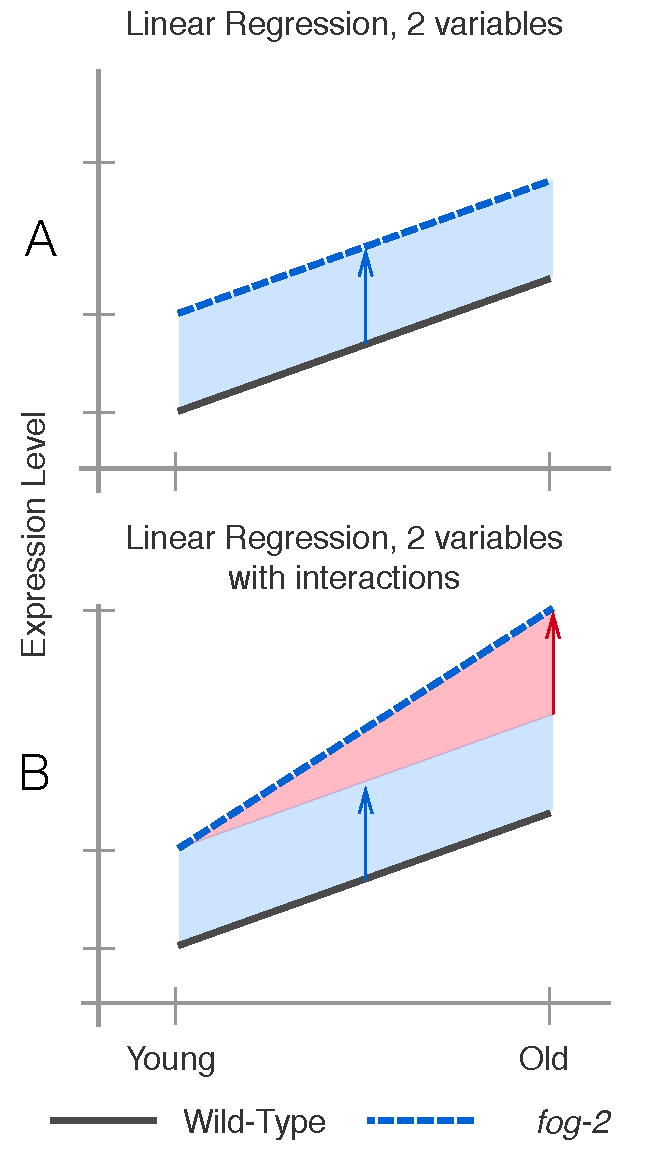
\includegraphics[width=0.5\linewidth]{femims/linear_regression.pdf}
\caption{
\textbf{A}. A linear regression with two variables, age and genotype.
The expression level of a gene increases by the same amount as worms age
regardless of genotype. However, \fog{} has more mRNA than the wild-type at all
stages (blue arrow).
\textbf{B}. A linear regression with two variables and an
interaction term. In this example, the expression level of this hypothetical
gene is different between wild-type worms and \fog{} (blue arrow). Although the
expression level of this gene increases with age, the slope is different between
wild-type and \fog{}. The difference in the slope can be accounted for through
an interaction coefficient (red arrow).
}
\label{fig:linear_reg}
\end{figure}

One way to analyze the data from this two-factor design is by pairwise
comparison of the distinct states. However, such an analysis would not make full
use of all the statistical power afforded by this experiment. Another method
that makes full use of the information in our experiment is to perform a linear
regression in 3 dimensions (2 independent variables, age and genotype, and 1
output). A linear regression with 1 parameter (age, for example) would fit a
line between expression data for young and old animals. When a second parameter
is added to the linear regression, said parameter can be visualized as altering
the y-intercept, but not the slope, of the first line in question (see
Fig.~\ref{fig:linear_reg}a).

Although a simple linear model is oftentimes useful, sometimes it is not
appropriate to assume that the two variables under study are entirely
independent. For example, in our case, three out of the four timepoint-and-genotype
combinations we studied did not have sperm, and sperm-status is
associated with both the \fog{} self-sterile phenotype and with biological age
of the wild-type animal. One way to statistically model such correlation between
variables is to add an interaction term to the linear regression.
This interaction term allows extra flexibility in describing how changes occur
between conditions.
For example, suppose a given theoretical gene \gene{X} has expression levels that
increase in a \gene{fog-2}-dependent manner, but also increases in an
age-dependent manner. However, aged \fog{} animals do not have expression levels
of \gene{X} that would be expected from adding the effect of the two perturbations;
instead, the expression levels of \gene{X} in this animal are considerably above
what is expected. In this case, we could add a positive
interaction coefficient to the model to explain the effect of genotype on the
y-intercept as well as the slope (see Fig.~\ref{fig:linear_reg}b).
When the two
perturbations are loss-of-function mutations, such interactions are epistatic
interactions.

For these reasons, we used a linear generalized model (see \nameref{sb:statistics})
with interactions to identify a transcriptomic profile associated with the
\fog{} genotype independently of age, as well as a transcriptomic profile of
\cel{} aging common to both genotypes. The change associated with each variable
is referred as $\beta$; this number, although related to the natural logarithm
of the fold change, is not equal to it. However, it is true that larger
magnitudes of $\beta$ indicate greater change. Thus, for each gene we performed
a linear regression, and we evaluated the whether the $\beta$ values associated
with each coefficient were significantly different from 0 via a Wald test
corrected for multiple hypothesis testing. A coefficient was considered to be
significantly different from 0 if the q-value associated with it was less than
0.1.

\subsection*{A quarter of all genes change expression between the 1st day of
             adulthood and the 6th day of adulthood in \cel{}.}
We identified a transcriptomic signature consisting of \agen{} genes that were
differentially expressed in 6th day adult animals of either genotype relative
to 1st day adult animals (see SI file 2). This constitutes more than one quarter
of the genes in \cel{}. Tissue Enrichment Analysis (TEA)~\citep{Angeles-Albores2016}
showed that nervous tissues including the `nerve ring', `dorsal nerve cord', `PVD'
and `labial sensillum' were enriched in genes that become differentially expressed
through aging. Likewise, certain muscle groups (`anal depressor muscle', `intestinal
muscle') were enriched. (see Figure~\ref{fig:agingtranscriptome}b). Gene
Enrichment Analysis (GEA)~\citep{Angeles-Albores106369} revealed that genes that
were differentially expressed during the course of aging were enriched in terms
involving respiration (`respiratory chain', `oxoacid metabolic process');
translation (`cytosolic large ribosomal subunit'); and nucleotide metabolism
(`purine nucleotide', `nucleoside phosphate' and `ribose phosphate' metabolic
process). Phenotype Enrichment Analysis (PEA)~\citep{Angeles-Albores106369} showed
enrichment of phenotypes that affect the \cel{} gonad, including `gonad vesiculated',
`gonad small', `oocytes lack nucleus' and `rachis narrow'.

To verify the quality of our dataset, we generated a list of \goldn{} golden
standard genes expected to be altered in 6th day adult worms using previous
literature reports including downstream genes of \gene{daf-12}, \gene{daf-16},
and aging and lifespan extension datasets~\citep{Murphy2003,Halaschek-wiener2005,
Lund2002,McCormick2012,Eckley2013}. Out of \goldn{} standard genes, we found
\goldfound{} genes in our time-responsive dataset. This result was statistically
significant with a p-value \goldpval{}.

Next, we used a published compendium~\citep{Reece-Hoyes2005} to search for known
or predicted transcription factors. We found \tfaging{} transcription factors in
the set of genes with differential expression in aging nematodes. We subjected
this list of transcription factors to TEA to understand their expression
patterns. 6 of these transcription factors were expressed in the `hermaphrodite
specific neuron' (HSN), a neuron physiologically relevant for egg-laying
(\gene{hlh-14}, \gene{sem-4}, \gene{ceh-20}, \gene{egl-46}, \gene{ceh-13},
\gene{hlh-3}), which represented a statistically significant 2-fold enrichment of
this tissue ($q<10^{-1}$). The term `head muscle' was also overrepresented at
twice the expected level ($q<10^{-1}$, 13 genes). Many of these transcription
factors have been  associated with developmental processess, and it is unclear
why they would change expression in adult animals.

\subsection*{The whole-organism \fog{} transcriptome in \cel{}.}
We identified \fogn{} genes associated with the \fog{} genotype, including
\tffog{} transcription factors (see SI file 3). TEA showed that the terms `AB',
`midbody', `uterine muscle', `cephalic sheath cell', `anal depressor muscle' and
`PVD' were enriched in this gene set. The terms `AB' and `midbody' likely reflect
the impact of \fog{} on the germline.
Phenotype enrichment showed that only a single phenotype, `spindle orientation
variant' was enriched in the \fog{} transcriptome ($q<10^{-1}$, 38 genes, 2-fold
enrichment). Most genes annotated as `spindle orientation variant' were
slightly upregulated, and therefore are unlikely to uniquely reflect reduced
germline proliferation. GO term enrichment was very similar to the aging gene
set and reflected enrichment in annotations pertaining to translation and
respiration. Unlike the aging gene set, the \fog{} transcriptome was
significantly enriched in `myofibril' and `G-protein coupled receptor binding'
($q<10^{-1}$). Enrichment of the term `G-protein coupled receptor binding' was
due to 14 genes: \gene{cam-1}, \gene{mom-2},  \gene{dsh-1}, \gene{spp-10},
\gene{flp-6}, \gene{flp-7}, \gene{flp-9}, \gene{flp-13}, \gene{flp-14},
\gene{flp-18},
\gene{K02A11.4}, \gene{nlp-12}, \gene{nlp-13}, and \gene{nlp-40}.
\gene{dsh-1},
\gene{mom-2} and \gene{cam-1} are members of the Wnt signaling pathway.
Most of these genes' expression levels were up-regulated, suggesting increased
G-protein binding activity in \fog{} mutants.

\subsection*{The \fog{} transcriptome overlaps significantly with the aging
transcriptome}
Of the \fogn{} genes that we identified in the \fog{}
transcriptome, \intersectn{} genes were also identified in our aging set.
Moreover, of these \intersectn{}  genes, \coexpressed{} genes changed in the
same direction in response either aging or germline feminization.
The overlap between these transcriptomes suggests an interplay between sperm-status
and age. The nature of the interplay should be captured by the interaction coefficients
in our model.
There are four possibilities. First, the \fog{} worms may
have a fast-aging phenotype, in which case the interaction coefficients should
match the sign of the aging coefficient.
Second, the \fog{} worms may
have a slow-aging phenotype, in which case the interaction coefficients should
have an interaction coefficient that is of opposite sign, but not greater in
magnitude than the aging coefficient (if a gene increases in aging in a
wild-type worm, it should still increase in a \fog{} worm, albeit less).
Third, the \fog{} worms exhibit a rejuvenation phenotype. If this is the case,
then these genes should have an interaction coefficient that is of opposite sign
and greater magnitude than their aging coefficient, such that the change of
these genes in \fog{} mutant worms is reversed relative to the wild-type.
Finally, if these genes are indicative of a female state, then these genes
should not change with age in \fog{} animals, since these animals do not exit
this state during the course of the experiment.
Moreover, because wild-type
worms become female as they age, a further requirement for a transcriptomic
signature of the female state is that aging coefficients for genes in this
signature should have genotype coefficients of equal sign and magnitude. In
other words, entrance into the female state should be not be path-dependent.


% aberrant aging
\begin{figure}
\renewcommand{\familydefault}{\sfdefault}\normalfont{}
\centering
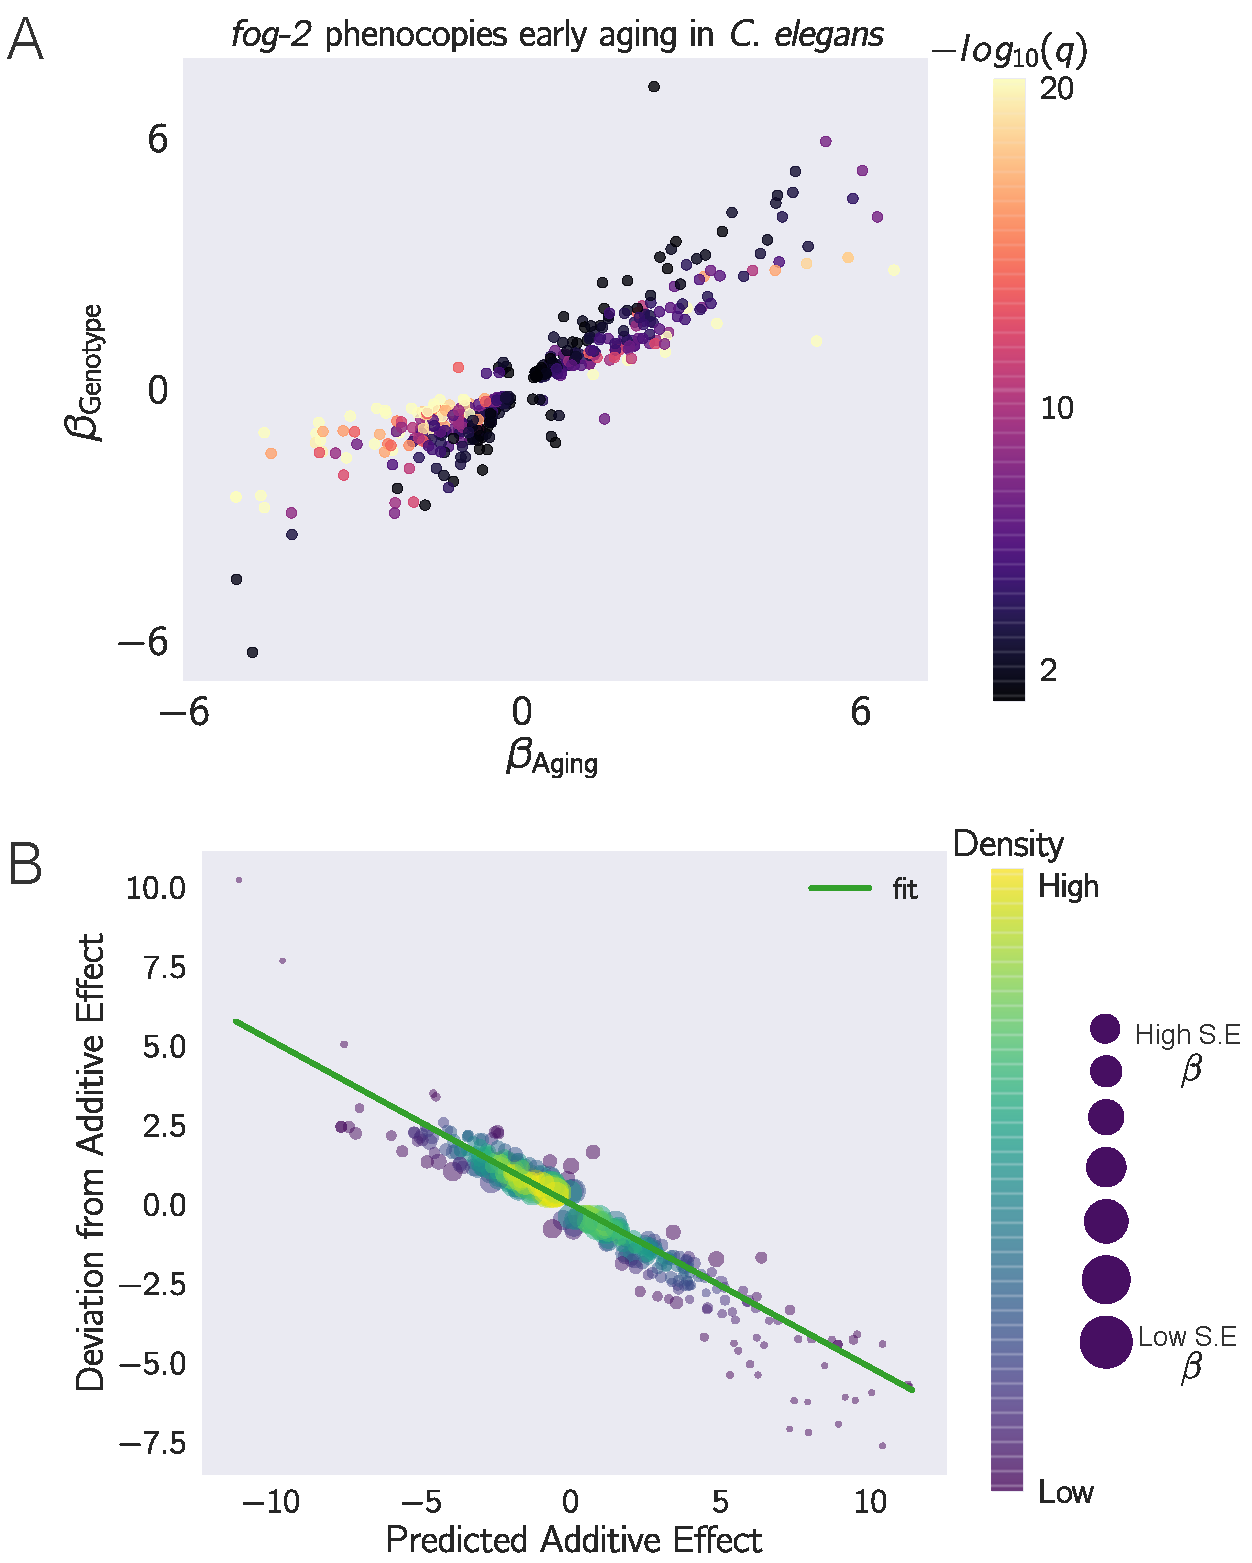
\includegraphics[width=0.7\linewidth]{femims/aberrant_aging.pdf}
\caption{
\fog{} partially phenocopies early aging in \cel{}. The $\beta$ in
each axes is the regression coefficient from the GLM, and can be loosely
interpreted as an estimator of the log-fold change.
Feminization by loss of \fog{} is associated with a transcriptomic phenotype
involving \fogn{} genes. \intersectn{}/\fogn{} of these genes are also altered
in wild-type worms as they progress from young adulthood to old adulthood, and
\coexpressed{} change in the same direction. However, progression from young to
old adulthood in a \fog{} background results in no change in the expression
level of these genes.
\textbf{A} We identified genes that change similarly during feminization and aging.
The correlation between feminization and aging is almost 1:1.
\textbf{B} Epistasis plot of aging versus feminization. Epistasis plots indicate
whether two genes (or perturbations) act on the same pathway. When two effects act
on the same pathway, this is reflected by a slope of $-0.5$. The measured slope
was $-0.51 \pm 0.01$.
}%
\label{fig:aberrant_aging}
\end{figure}

To evaluate which of these possibilities was most likely, we selected
the \intersectn{} genes that had aging, genotype and interaction coefficients
significantly different from zero and we plotted their temporal coefficients
against their genotype coefficients (see Fig.~\ref{fig:aberrant_aging}a). We
observed that the aging coefficients were strongly predictive of the genotype
coefficients. Most of these genes fell near the line $y=x$, suggesting that these
genes define a female state. As a further test that these genes actually define
a female state, we generated an epistasis plot using this gene set. We have
previously used epistasis plots to measure transcriptome-wide epistasis between
genes in a pathway~\citep{}.
Briefly, an epistasis plot plots the expected expression of a double perturbation
under an additive model (null model) on the x-axis, and the deviation from this
null model in the y-axis. In other words, we calculated the x-coordinates for each
point by adding $\beta_\mathrm{Genotype} + \beta_\mathrm{Aging}$, and the
y-coordinates are equal to $\beta_{Interaction}$ for each isoform.
Previously we have shown that if two genes act in a
linear pathway, an epistasis plot will generate a line with slope equal to $-0.5$.
When we generated an epistasis plot and found the line of best fit, we observed
a slope of $-0.51\pm 0.01$, which suggests that the \gene{fog-2} gene and time
are acting to generate a single transcriptomic phenotype along a single pathway.
Overall, we identified
\femalen{} genes that increased in the same direction through age or mutation
of the \fog{} gene and that had an interaction coefficient of opposite sign to
the aging or genotype coefficient (see SI file 4). Taken together, this
information suggests that these \femalen{} genes define a female state in
\cel{}.

\subsection*{Analysis of the Female State Transcriptome}

\begin{figure}
  \renewcommand{\familydefault}{\sfdefault}\normalfont{}
  \centering
  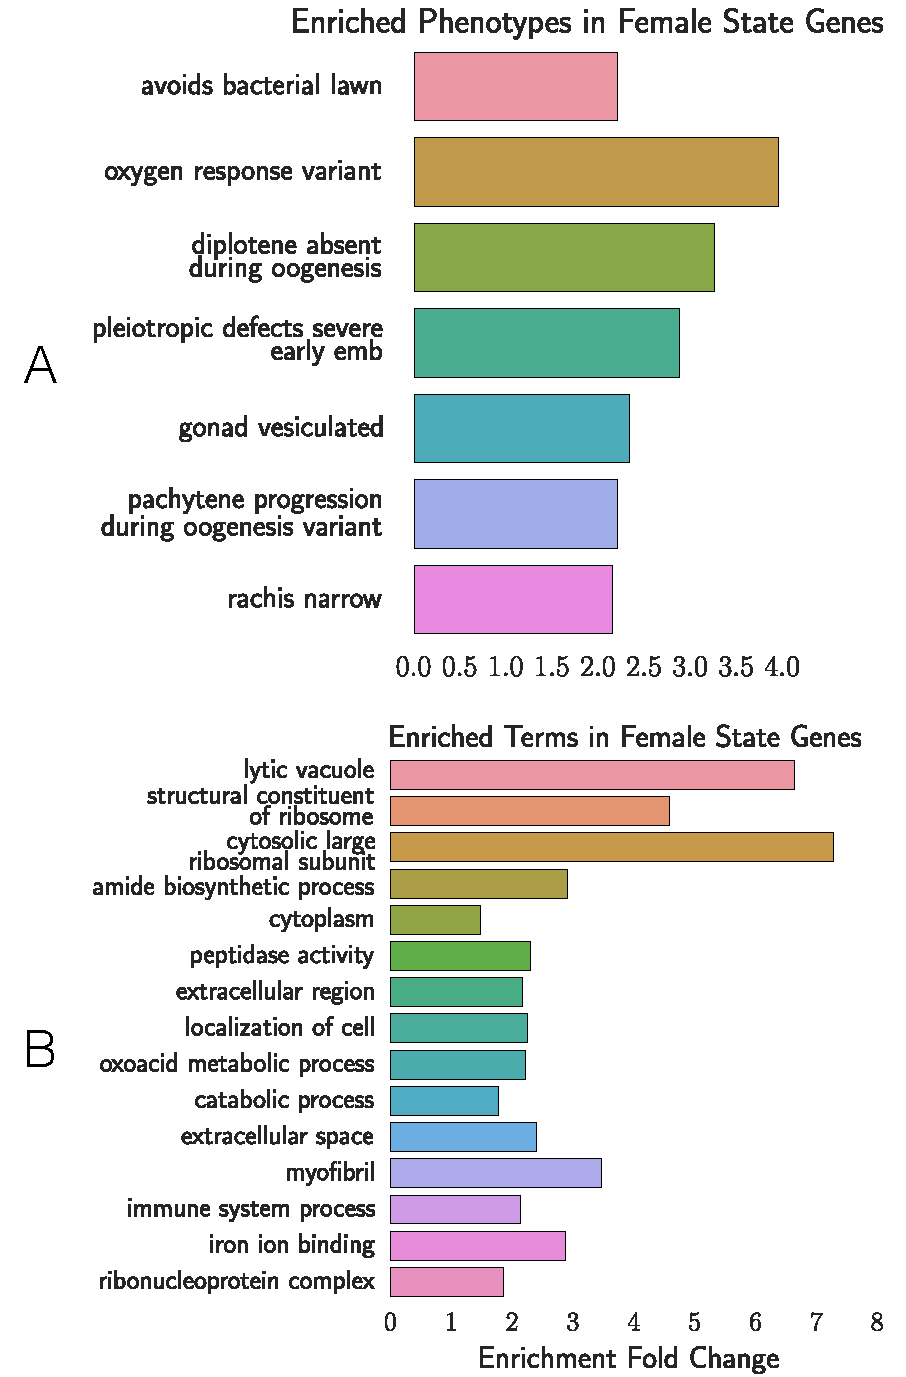
\includegraphics[width=0.55\linewidth]
  {femims/female_state_enrichment.pdf}
  \caption{
  Phenotype and GO enrichment of genes involved in the female state.
  \textbf{A}. Phenotype Enrichment Analysis.
  \textbf{B}. Gene Ontology Enrichment Analysis.
  Most of the terms enriched in PEA reflect the abundance of ribosomal subunits
  present in this gene set.
  }
\label{fig:female_state_enrich}
\end{figure}

To better understand the changes that happen after sperm loss, we performed
tissue enrichment, phenotype enrichment and gene ontology enrichment analyses
on the set of \femalen{} genes that we associated with the female state.
TEA showed no tissue enrichment using this gene-set. GEA
showed that this gene list was enriched in constituents of the ribosomal
subunits almost four times above background ($q<10^{-5}$, 17 genes). The
enrichment of ribosomal constituents in this gene set in turn drives the
enriched phenotypes: `avoids bacterial lawn',
`diplotene absent during oogenesis', `gonad vesiculated', `pachytene progression
during oogenesis variant', and `rachis narrow'. The expression of most of these
ribosomal subunits is down-regulated in aged animals or in \fog{} mutants.

\section*{Discussion}
\label{sec:discussion}

\subsection*{Defining an Early Aging Phenotype}
\label{sub:Defining an Early Aging Phenotype}

Our experimental design enables us to decouple the effects of egg-laying from
aging. As a result, we identified a set of almost 4,000 genes that are altered
similarly between wild-type and \fog{} mutants. Due to the read depth of our
transcriptomic data (20 million reads) and the number of samples measured (3
biological replicates for 4 different life stages/genotypes), this dataset
constitutes a high-quality description of the transcriptomic changes that occur
in aging populations of \cel{}.
Although our data only capture $\sim50\%$ of the expression changes reported
in earlier aging transcriptome literature, this disagreement can be explained
by a difference in methodology; earlier publications typically addressed the
aging of fertile wild-type hermaphrodites only indirectly, or queried aging
animals at a much later stage of their life cycle.


\subsection*{Measurement of a female state is enabled by linear models}
\label{sub:female_state}

We set out to study the self-fertilizing (hermaphroditic) to self-sterile
(female) transition by comparing wild-type animals with \fog{} mutants as they
aged. Our computational approach enabled us to separate between two biological
processes that are correlated within samples. Because of this intra-sample
correlation, identifying this state via pairwise comparisons would not have been
straightforward. Although it is a favored method amongst biologists, such
pairwise comparisons suffer from a number of drawbacks.
First, pairwise comparisons are unable to draw on the full statistical power
available to an experiment because they discard almost all information except
the samples being compared. Second, pairwise comparisons require a researcher
to define \emph{a priori} which comparisons are informative. For experiments
with many variables, the number of pairwise combinations is explosively large.
Indeed, even for this two-factor experiment, there are 6 possible pairwise
comparisons. On the other hand, by specifying a linear regression model, each
gene can be summarized with three variables, each of which can be analyzed and
understood without the need to resort to further pairwise combinations.

Our explorations have shown that the loss of \fog{} partially phenocopies the
transcriptional events that occur naturally as \cel{} ages from the 1st day of
adulthood to the 6th day of adulthood. Moreover, epistasis analysis of these
perturbations suggest that they act on the same pathway, namely sperm generation
and depletion (see Fig.~\ref{fig:lifecycle}). Sperm generation promotes a non-female
states, whereas sperm depletion causes entry into the female state. Given the
enrichment of neuronal transcription factors that are associated with sperm loss
in our dataset, we believe this dataset should contain some of the transcriptomic
modules that are involved in these pheromone production and behavioral pathways,
although we have been unable to find these genes. Currently, we cannot judge how
many of the changes induced by loss of hermaphroditic sperm are developmental
(i.e., irreversible), and how many can be rescued by mating to a male.
While an entertaining thought experiment, establishing whether these transcriptomic
changes can be rescued by males is a daunting experimental task, given that the
timescales for physiologic changes could reasonably be the same as the timescale
of onset of embryonic transcription. All in all, our research supports the idea
that wide-ranging transcriptomic effects of aging in various tissues can be
observed well before onset of mortality, and that \cel{} continues to develop as
it enters a new state of its life cycle.

\subsection*{The \cel{} life cycle, life stages and life states}

\begin{figure}
\renewcommand{\familydefault}{\sfdefault}\normalfont{}
\centering
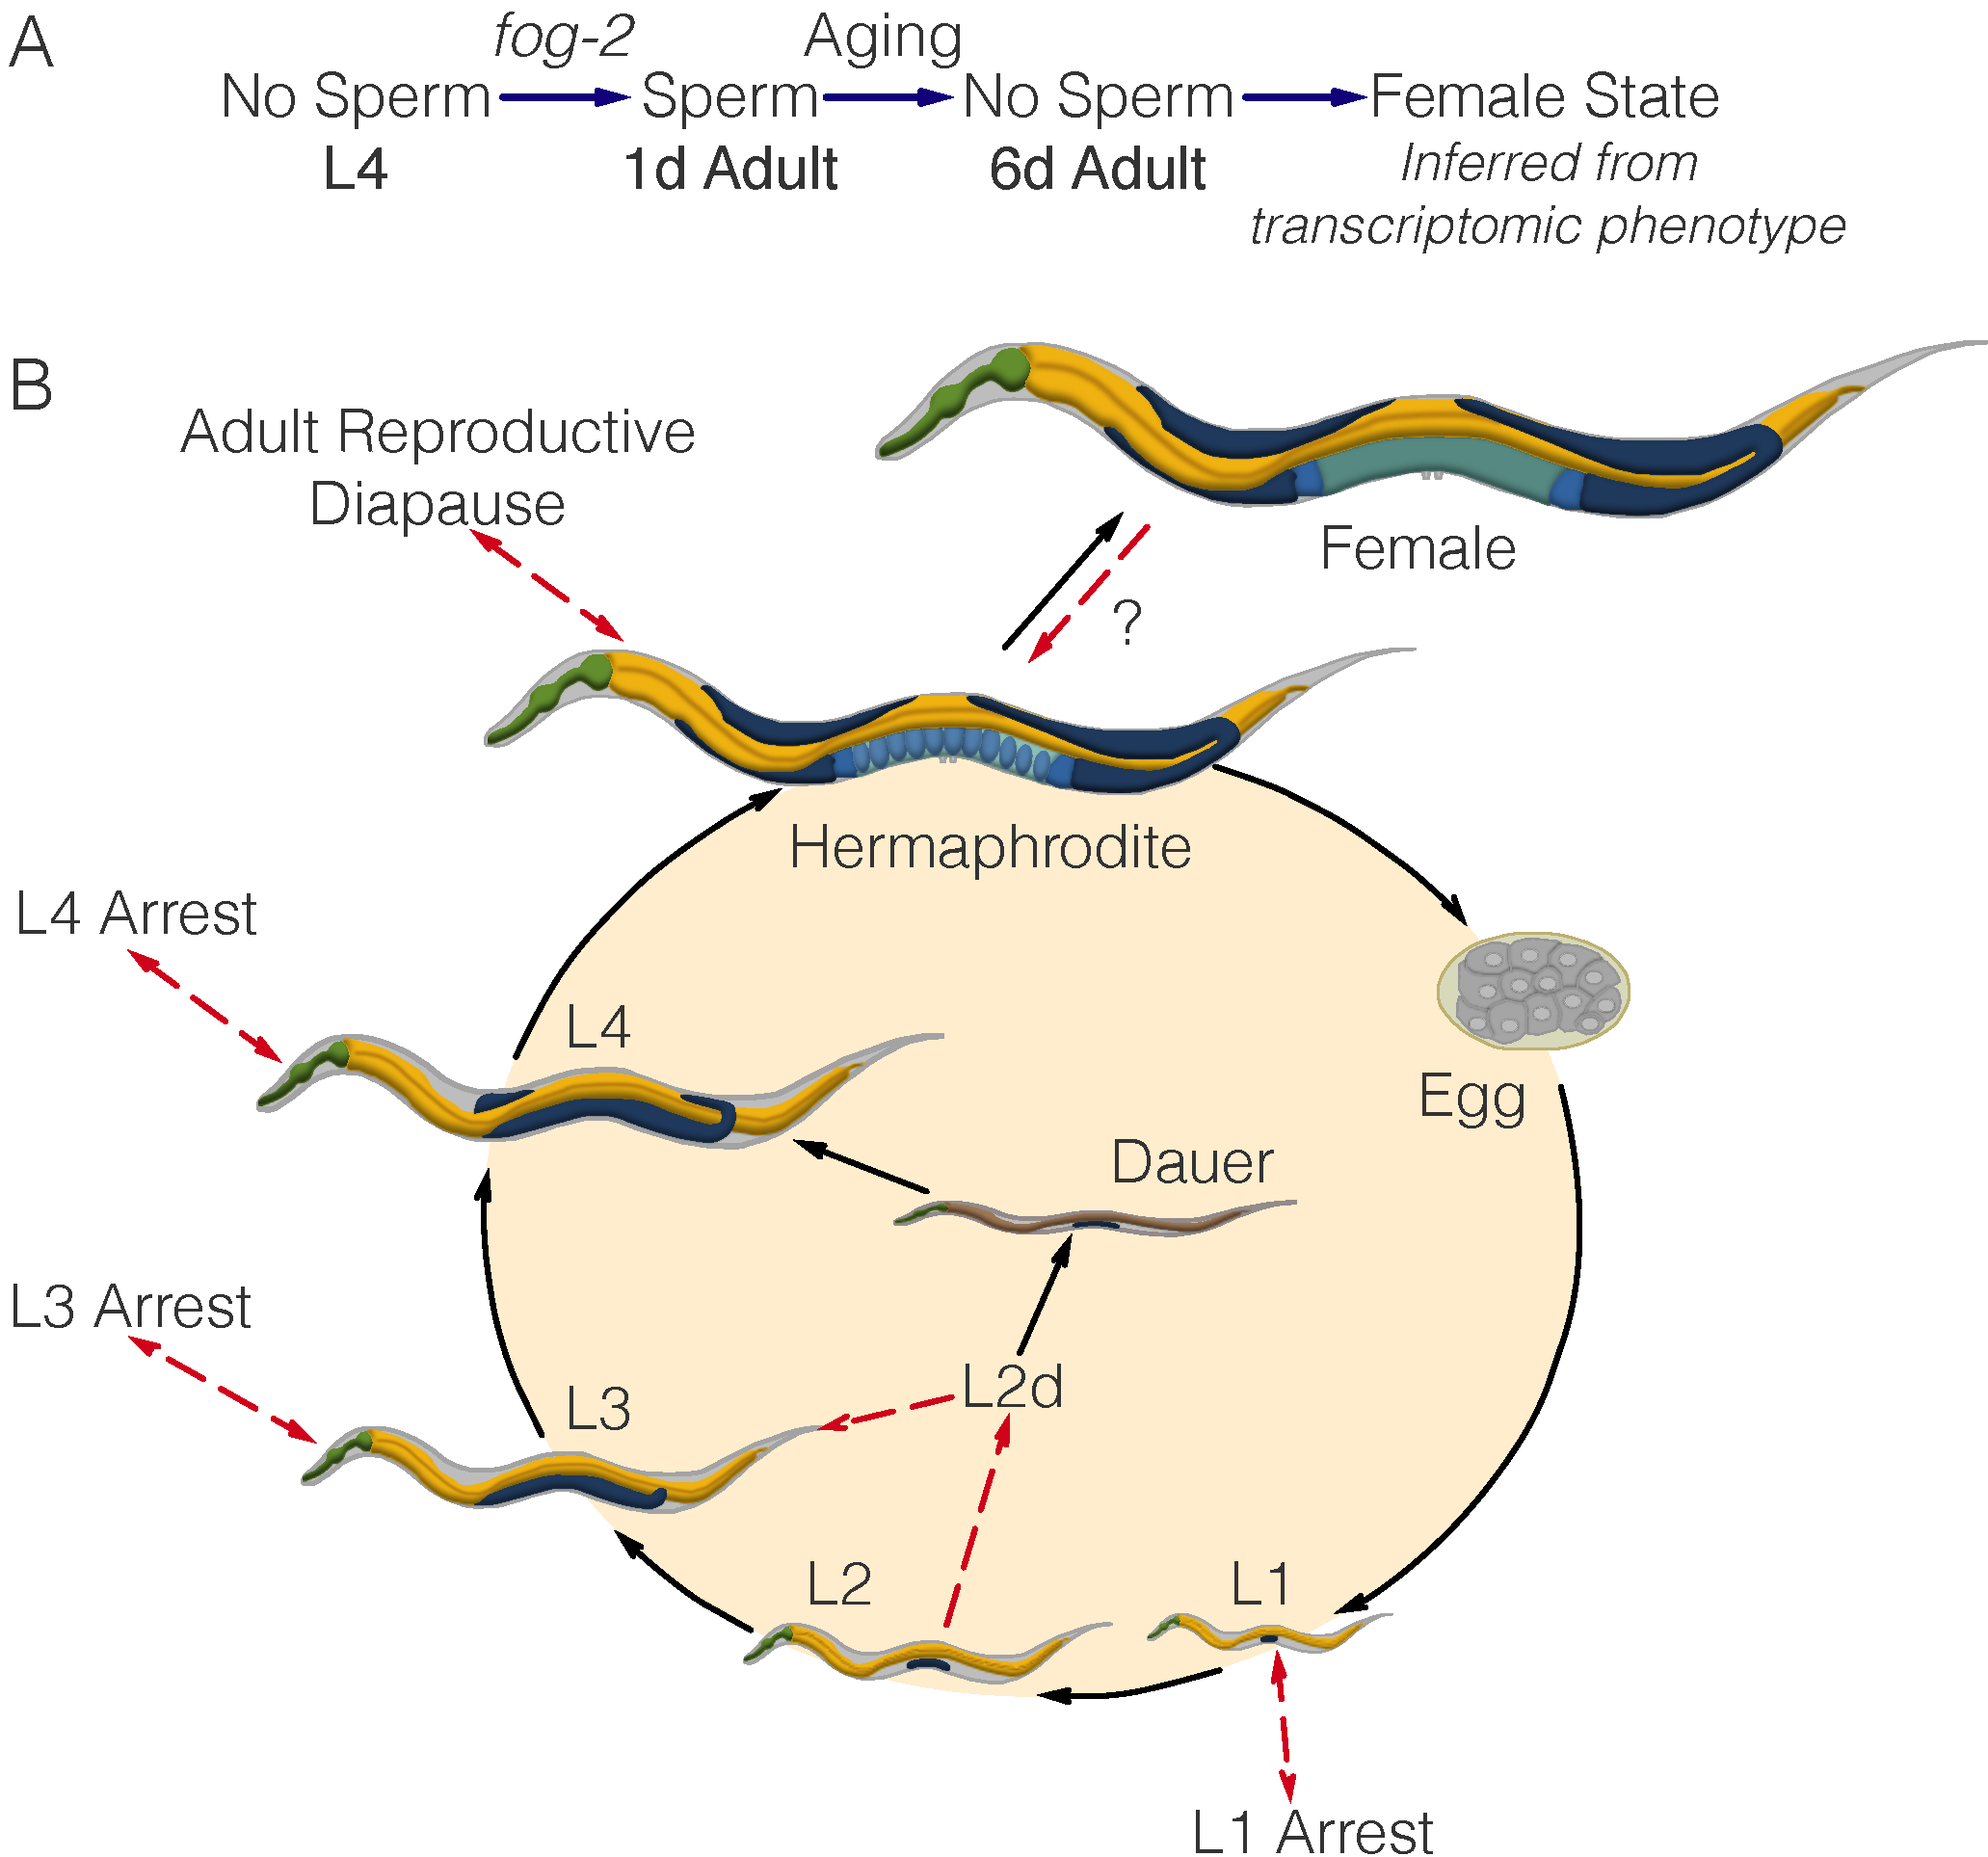
\includegraphics[width=0.5\linewidth]{femims/c_elegans_life_cycle.pdf}
\caption{
\textbf{A}. A substrate model showing how \gene{fog-2} promotes sperm generation,
whereas aging promotes sperm depletion, leading to entry to the female state. Such
a model can explain why \gene{fog-2} and aging appear epistatic to each other.
\textbf{B}.
The complete \cel{} life cycle. Recognized stages of \cel{} are marked by black
arrows. States are marked by red arrows to emphasize that at the end of a state,
the worm returns to the developmental timepoint it was at before entering the
state. The L2d state is an exception. It is the only stage that does not return
to the same developmental timepoint; rather, the L2d state is a permissive state
that allows entry into either dauer or the L3 stage. We have presented evidence
of a female state in \cel{}. At this point, it is unclear whether the difference
between hermaphrodites and females is reversible by males. Therefore, it remains
unclear whether it is a stage or a true state.
}%
\label{fig:lifecycle}
\end{figure}

\cel{} has a complicated life cycle, with two alternative developmental pathways
that have multiple stages (larval development and dauer development), followed
by reproductive adulthood. In addition to its developmental stages, researchers
have recognized that \cel{} has numerous life states that it can enter into when
given instructive environmental cues. One such state is the L1 arrest state,
where development ceases entirely upon starvation~\citep{Johnson1984}. More
recently, researchers have described additional diapause states that the worm
can access at the L3, L4 and young adult stages under conditions of low
food~\citep{Angelo2009,Seidel2011,Schindler2014}. Not all states of \cel{} are
arrested, however (see Fig.~\ref{fig:lifecycle}). For example, the L2d state is
induced by crowded and nutrient poor conditions~\citep{Golden1984}. While within
this state, the worm is capable of entry into either dauer or the L3 larval
stage, depending on environmental conditions. Thus, the L2d state is a
permissive state, and marks the point at which the nematode development is
committed to a single developmental pathway.

Identification of the \cel{} life states has often been performed by
morphological studies (as in the course of L4 arrest or L2d) or via
timecourses (L1 arrest). However, not all states may be visually identifiable,
or even if they are, the morphological changes may be very subtle, making
positive identification difficult. However, the detailed information afforded
by a transcriptome should in theory provide sufficient information to
definitively identify a state, since transcriptomic information underlies
morphology. Moreover, transcriptomics can provide an informative description
into the physiology of complex metazoan life state's via measurements of global
gene expression. By identifying differentially expressed genes and using
ontology enrichment analyses to identify gene functions, sites of expression
or phenotypes that are enriched in a given gene set, researchers can obtain a
clearer picture of the changes that occur in the worm in a less biased manner
than by identifying gross morphological changes.
RNA-seq is emerging as a powerful technology that has been used successfully in
the past as a qualitative tool for target acquisition. More recent work has
successfully used RNA-seq to establish genetic interactions between
genes~\citep{Dixit2016,Adamson2016}.
In this work, we have shown that whole-organism RNA-seq data can also be analyzed
via a similar formalism to successfully identify internal states in a
multi-cellular organism.

% \subsection*{mRNA Levels of Developmental Factors Change Between 1st
%              to 6th Day of Adulthood in \cel{}}
% \label{sub:development_in_aging}
%
% Our transcriptomes reveal a host of transcription factors that changed between
% the 1st and 6th day of adulthood in \cel{}. Many of these transcription factors
% have been associated with development via cellular differentiation and
% specification. For example, we identified the transcription factor
% \emph{lin-32}, which has been associated with neuron
% development~\citep{Chalfie1989,Zhao1995,Portman2000}; the Six5 ortholog
% \emph{unc-39} has been associated with axonal pathfinding and neuron
% migration\citep{Manser1990,Yanowitz2004}; \emph{cnd-1}, a homolog  of the
% vertebrate NeuroD transcription factors, is expressed in the early embryo and is
% also involved in axon guidance~\citep{Schmitz2007}.
% Why these transcription factors increase their expression is a mystery,
% but we speculate that this hints at important neuronal changes that are
% taking place.


% \section*{Acknowledgments}
%
% We thank the \emph{Caenorhabditis} Genetics Center for providing worm strains.
% This work would not be possible without the central repository of \cel{}
% information generated by WormBase, without which mining the genetic data would
% not have been possible. DHWL was supported by a National Institutes of Health
% US Public Health Service Training Grant (T32GM07616). This research was
% supported by the Howard Hughes Medical Institute, for which PWS is an
% investigator.

% \subsubsection*{Author Contributions:}
% DA, DHWL and PWS designed all experiments. DHWL and THK collected RNA for
% library preparation. IA generated libraries and performed sequencing.
% DA performed all bioinformatics and statistical analyses.
% DA, TT and DHWL performed all screens. DA, DHWL and PWS wrote the paper.
%
%
% \bibliography{citations}

  \printbibliography[heading=subbibliography]
\end{refsection}

\chapter{Understanding the SynMuv phenotype from a transcriptomic perspective}
\begin{refsection}
  % \newcommand{\dicty}{\emph{D.~discoideum}}

% gene names
\newcommand{\nlp}{\emph{\mbox{nlp-31}}}
\newcommand{\ftna}{\emph{\mbox{ftn-1}}}
\newcommand{\ftnb}{\emph{\mbox{ftn-2}}}
\newcommand{\cysl}{\emph{\mbox{cysl-1}}}
\newcommand{\nog}{\emph{\mbox{nog-1}}}
\newcommand{\nhr}{\emph{\mbox{nhr-57}}}
\newcommand{\lam}{\emph{\mbox{lam-3}}}

\newcommand{\fog}{\emph{\mbox{fog-2(lf)}}}
\newcommand{\egl}{\emph{\mbox{egl-9}(lf)}}
\newcommand{\rhy}{\emph{\mbox{rhy-1}(lf)}}
\newcommand{\vhl}{\emph{\mbox{vhl-1}(lf)}}
\newcommand{\eglvhl}{\emph{\mbox{egl-9(lf);vhl-1(lf)}}}
\newcommand{\eglhif}{\emph{\mbox{egl-9(lf)}~\mbox{hif-1(lf)}}}
\newcommand{\hif}{\emph{\mbox{hif-1(lf)}}}

% protein names
\newcommand{\eglp}{EGL-9}
\newcommand{\rhyp}{RHY-1}
\newcommand{\nogp}{NOG-1}
\newcommand{\vhlp}{VHL-1}
\newcommand{\hifp}{HIF-1}
\newcommand{\fogp}{FOG-2}
\newcommand{\nhrp}{NHR-57}
\newcommand{\lamp}{LAM-3}
\newcommand{\cyslp}{CYSL-1}

% DE genes numbers:
\newcommand{\egln}{1,806}
\newcommand{\rhyn}{2,103}
\newcommand{\vhln}{689}
\newcommand{\eglvhln}{2,376}
\newcommand{\hifn}{546}
\newcommand{\eglhifn}{404}
\newcommand{\fogn}{2090}
\newcommand{\total}{5,671} % isoforms!!!!
% \newcommand{\inall}{53}
% \newcommand{\allup}{10}
% \newcommand{\alldown}{13}

% downstream targets
\newcommand{\egltargets}{126}
\newcommand{\rhytargets}{0}
\newcommand{\vhltargets}{45} % 44 genes, minus vhl-1 (IDed due to deletion)
\newcommand{\hiftargets}{195}
\newcommand{\hifohtargets}{31}


% website commands
\newcommand{\website}{
            \url{https://wormlabcaltech.github.io/Angeles_Leighton_2016/}
            }
\newcommand{\webref}{
\href{https://wormlabcaltech.github.io/Angeles_Leighton_2016/}{website}}

% more space between rows
\newcommand{\ra}[1]{\renewcommand{\arraystretch}{#1}}

\section*{Abstract}
\textbf{
RNA-seq is commonly used to identify genetic modules that respond to perturbations.
In single cells, transcriptomes have been used as phenotypes, but this concept
has not been applied to whole-organism RNA-seq. Linear models can quantify
expression effects of individual mutants and identify epistatic effects in double
mutants. However, interpreting these high-dimensional measurements is unintuitive.
We developed a single coefficient to quantify transcriptome-wide epistasis which
accurately reflects the underlying interactions. To demonstrate the power of our
approach, we sequenced four single and two double C. elegans mutants. From these
mutants, we successfully reconstructed the known hypoxia pathway. Using this
approach, we uncovered a class of 31 genes that have opposing changes in expression
in \egl{} and \vhl{} but the \eglvhl{} mutant phenocopies \egl{}.
These changes violate the classical model of HIF-1 regulation, but can be explained
by postulating a role of hydroxylated HIF-1 in transcriptional control.
}
\vspace{10mm}


\section*{Introduction}
\label{sec:introduction}
Genetic analysis of molecular pathways has traditionally been performed
through epistatis analysis. Generalized epistasis indicates that two genes interact
functionally; such interaction can involve the direct interaction of their
products or the interaction of any consequence of their function (small molecules,
physiological or behavioral effects)~\citep{Huang2006}. If two
genes interact, and the mutants of these genes have a quantifiable phenotype,
the double mutant of interacting genes will have a phenotype that is not the sum
of the phenotypes of the single mutants that make up its genotype. Epistasis
analysis remains a cornerstone of genetics today~\citep{Phillips2008}.


Recently, biological studies have shifted in focus from studying single
genes to studying all genes in parallel. In particular,
RNA-seq~\citep{Mortazavi2008} enables biologists to
identify genes that change expression in response to a perturbation. Gene expression
profiling using RNA-seq has become much more sensitive thanks to deeper and more
frequent sequencing due to lower sequencing costs~\citep{Metzker2010},
better and faster abundance quantification~\citep{Patro2014,Bray2016,Patro2015},
and improved differential expression analysis
methods~\citep{Pimentel2016,Trapnell2013}. RNA-seq has been
successfully used to identify genetic modules involved in a variety of processes,
including T-cell regulation~\citep{Singer2016,Shalek2013}, the
\emph{Caenorhabditis~elegans} (\cel{}) linker
cell migration~\citep{Schwarz2012}, and planarian stem cell
maintenance~\citep{VanWolfswinkel2014,Scimone2014}. For the most part, the role of
transcriptional profiling has been restricted to target gene identification.

Although transcriptional profiling has been primarily used for descriptive purposes,
transcriptomic phenotypes have previously been used to make genetic inferences.
Microarray analyses in \emph{S. cerevisiae} and \dicty{} were used to show
that transcriptomes can be interpreted to infer genetic relationships in simple
eukaryotes~\citep{Hughes2000, VanDriessche2005}.\@ eQTL studies in
many organisms, from yeast to humans, have established the usefulness of
transcriptomic phenotypes for population genetics studies~\citep{Brem2002,Schadt2003,
Li2006,King2014}. In cell culture, single-cell RNA-seq has seen significant
progress towards using transcriptomes as phenotypes with which to test genetic
interactions~\citep{Adamson2016,Dixit2016}.
More recently, we have identified a new developmental state
of \cel{} using whole-organism transcriptome profiling~\citep{Angeles-Albores2016a}.
To investigate the ability of whole-organism transcriptomes to serve as quantitative
phenotypes for epistasis analysis in metazoans, we sequenced the transcriptomes of
of four well-characterized loss of function mutants in the \cel{} hypoxia
pathway~\citep{Epstein2001,Shen2006,Shao2009,Jiang2001}.

% carmie:
Metazoans depend on the presence of oxygen in sufficient concentrations to
support aerobic metabolism. Genetic pathways evolved to rapidly respond to any
acute or chronic changes in oxygen levels at the cellular or organismal level.
Biochemical and genetic approaches identified the Hypoxia Inducible Factors
(HIFs) as an important group of oxygen-responsive genes that are involved in a
broad range of human pathologies~\citep{Semenza2012}.

Hypoxia Inducible Factors are highly conserved in metazoans~\citep{Loenarz2011}.
A common mechanism for hypoxia-response induction is heterodimerization between a
HIF$\alpha$ and a HIF$\beta$ subunit; the heterodimer then initiates
transcription of target genes~\citep{Jiang1996}. The number and complexity of
HIFs varies throughout metazoans, with humans having three HIF$\alpha$ subunits
and two HIF$\beta$ subunits, whereas in the roundworm \cel{} there is a single
HIF$\alpha$ gene, \gene{hif-1}~\citep{Jiang2001} and a single HIF$\beta$
gene, \gene{ahr-1}~\citep{Powell-Coffman1998}. HIF target genes have been implicated
in a wide variety of cellular and extracellular processes including glycolysis,
extracellular matrix modification, autophagy and immunity~\citep{Semenza1994,
Bishop2004,Shen2005,Bellier2009,Semenza2012}.

Levels of HIF$\alpha$ proteins tend to be tightly regulated. Under conditions of
normoxia, \hifp{}$\alpha$ exists in the cytoplasm and partakes in a futile cycle
of continuous protein production and rapid degradation~\citep{Huang1996}.
\hifp{}$\alpha$ is hydroxylated by three proline hydroxylases
in humans (PHD1, PHD2 and PHD3) but is only hydroxylated by one proline
hydroxylase (\eglp{}) in \cel{}~\citep{Kaelin2008}. \hifp{} hydroxylation
increases its binding affinity to Von Hippel Lindau Tumor Suppressor 1
(\vhlp{}), which allows ubiquitination of \hifp{} leading to its subsequent
degradation. In \cel{}, \eglp{} activity is inhibited by binding of \cyslp{},
and \cyslp{} activity is in turn inhibited at the protein level by \rhyp{},
possibly by post-translational modifications to \cyslp{}~\citep{Ma2012} (see
Fig.~\ref{fig:pathway}).

% heatmap
\begin{figure}[tbhp]
\centering
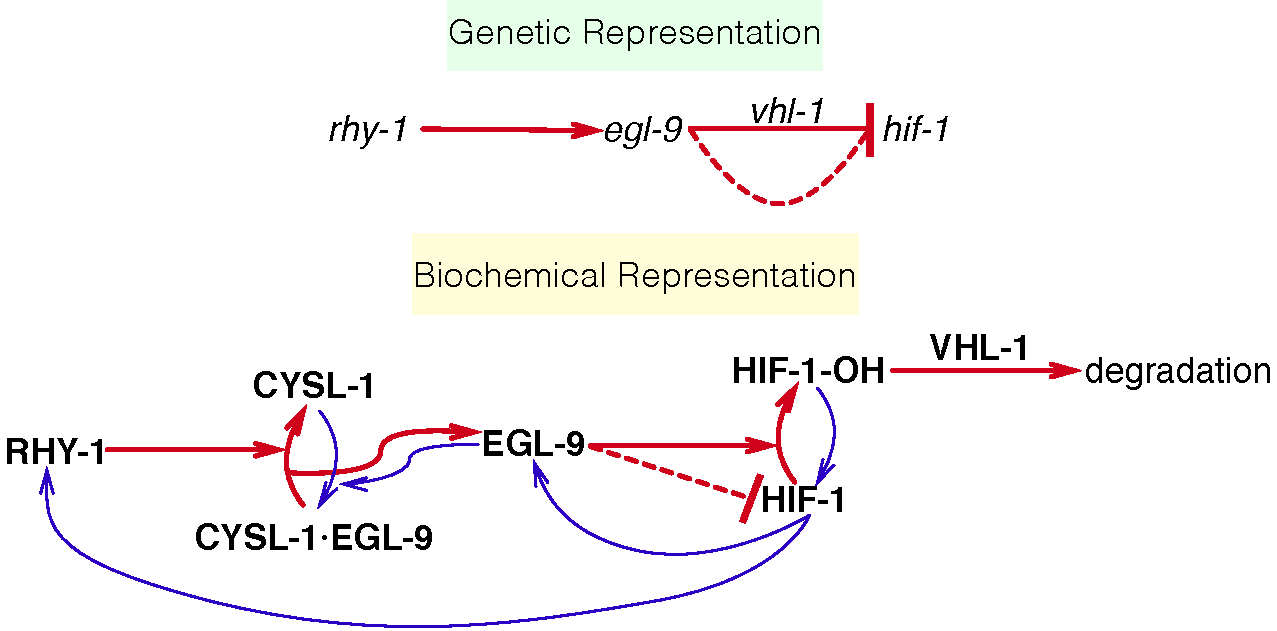
\includegraphics[width=.7\linewidth]{hypims/HIF1pathway.pdf}
\caption{
Genetic and biochemical representation of the hypoxia pathway in \cel{}.
Red arrows are arrows that lead to inhibition of \hifp{}, and blue arrows
are arrows that increase \hifp{} activity or are the result of \hifp{} activity.
\eglp{} is known to exert \gene{vhl-1}-dependent and independent repression
on \hifp{} as shown in the genetic diagram. The \gene{vhl-1}-independent
repression of \hifp{} by \eglp{} is denoted by a dashed line and is not dependent
on the hydroxylating activity of \eglp{}.
Technically, RHY-1 inhibits CYSL-1, which in turn inhibits EGL-9, but this
interaction was abbreviated in the genetic diagram for clarity.
}
\label{fig:pathway}
\end{figure}

Here, we show that transcriptomes contain robust signals that can be
used to infer relationships between genes in complex metazoans by reconstructing
the hypoxia pathway in \cel{} using RNA-seq.
Furthermore, we show that the phenomenon of phenotypic epistasis, a hallmark of
genetic interaction, holds at the molecular systems level.
We also demonstrate that transcriptomes contain sufficient information, under
certain circumstances, to order genes in a pathway using only single mutants.
Finally, we were able to identify genes that appear to be downstream of \gene{egl-9}
and \gene{vhl-1}, but do not appear to be targets of \gene{hif-1}.
Using a single set of genome-wide measurements, we were able to observe and
quantitatively assess  significant fraction of the known transcriptional
effects of \gene{hif-1} in \cel{}.
A complete version of the analysis, with ample documentation, is available at
\url{https://wormlabcaltech.github.io/mprsq}.

\section*{Results}
\subsection*{The hypoxia pathway controls thousands of genes in \cel{}}
\label{sub:summary}

We selected four single mutants within the hypoxia pathway for expression profiling:
\egl{} (\emph{sa307}), \rhy{} (\emph{ok1402}), \vhl{} (\emph{ok161}), \hif{} (\emph{ia4}).
We also sequenced the transcriptomes of two double mutants, \eglvhl{} (\emph{sa307},
\emph{ok161}) and \eglhif{} (\emph{sa307}, \emph{ia4}) as well as wild-type N2 as
a control sample. Each genotype  was sequenced in triplicate at a depth of 15
million reads. We performed whole-organism RNA-seq of these mutants at a moderate
sequencing depth ($\sim7$ million mapped reads for each individual replicate)
under normoxic conditions. For single samples, we identified around 22,000 different
isoforms per sample, which allowed us to measure differential expression of 18,344
isoforms across all replicates and genotypes (this constitutes  $\sim$70\% of
the protein coding isoforms in \cel{}).
We also included in our analysis a \fog{} (\emph{q71}) mutant which we have previously
studied~\citep{Angeles-Albores2016a}, because \gene{fog-2} is not reported to
interact with the hypoxia pathway.
We analyzed our data using a general linear model on
logarithm-transformed counts. Changes in gene expression are reflected in the
regression coefficient, $\beta$ which is specific to each isoform within a genotype.
Statistical significance is achieved when the q-values for each $\beta$ (p-values
adjusted for multiple testing) are less than 0.1. Genes that are significantly
altered between wild-type and a given mutant have $\beta$ values that are
statistically significantly different from 0.  These coefficients are not equal
to the average log-fold change per gene, although they are loosely related to
this quantity. Larger magnitudes of $\beta$ correspond to larger perturbations.
These coefficients can be used to study the RNA-seq data in question.

In spite of the moderate sequencing depth, transcriptome profiling of the hypoxia
pathway revealed that this pathway controls thousands of genes in \cel{}. The
\egl{} transcriptome showed differential expression of \egln{} genes. Similarly,
\rhyn{} genes were differentially expressed in \rhy{} mutants. The \vhl{}
transcriptome showed considerably fewer differentially expressed genes (\vhln{}),
possibly because it is a weaker controller of \hif{} than
\egl{}~\citep{Shao2009}. The \egl{};\vhl{} double mutant transcriptome showed
\eglvhln{} differentially expressed genes. The \hif{} mutant also showed a
transcriptomic phenotype involving \hifn{} genes. The \eglhif{} double mutant
showed a similar number of genes with altered expression (\eglhifn{} genes, see
Table~\ref{tab:genes}).

\begin{table}[tbhp]
  \centering
  \begin{tabular}{lr}
    \toprule{}
    Genotype & Differentially Expressed Genes \\
    \midrule{}
    \egl{} & \egln{}\\
    \rhy{} & \rhyn{}\\
    \vhl{} & \vhln{}\\
    \eglvhl{} & \eglvhln{}\\
    \eglhif{} & \eglhifn{}\\
    \fog{} & \fogn{}\\
    \bottomrule{}
  \end{tabular}
  \caption{Number of differentially expressed genes in each mutant.}
\label{tab:genes}
\end{table}

\subsection*{Principal Component Analysis visualizes epistatic relationships between genotypes}
\label{sub:Clustering}

Principal Component Analysis (PCA) is a well-known technique in bioinformatics that is
used to identify relationships between high dimensional data points~\citep{Yeung2001}
We performed PCA on our data to examine whether each genotype clustered in a biologically
relevant manner. PCA identifies the vector that can explain most of the variation
in the data;this is called the first PCA dimension. Using PCA, one can identify
the first $n$ dimensions that can explain more than 95\% of the variation in the
data. Sample clustering in these $n$ dimensions often indicates biological
relationships between the data, although interpreting PCA dimensions can be
difficult.

After applying PCA, we expected \hif{} to cluster near \eglhif{}, because
\hif{} exhibits no phenotypic defects under normoxic conditions, in contrast to
\egl{}, which exhibits an egg-laying (Egl) phenotype in the same environment.
In \eglhif{} mutants the Egl phenotype of \egl{} mutants is suppressed and instead
the grossly wild-type phenotype of \hif{} is observed. On the other hand, we
expected \egl{}, \rhy{}, \vhl{} and \eglvhl{} to form a separate cluster since
each of these genotypes is Egl and has a constitutive hypoxic response. Finally,
we included as a negative control a \fog{} mutant we have analyzed
previously~\citep{Angeles-Albores2016a}. This data was obtained at a different
time from the other genotypes, so we included a batch-normalization term in our
equations to account for this. Since \gene{fog-2} has not been described
to interact with the hypoxia pathway, we expected that it should appear far away
from either cluster.

The first dimension of the PCA analysis was able to discriminate between mutants
that have constitutive high levels of \hifp{} and mutants that have no \hifp{},
whereas the second dimension was able to discriminate between mutants within the
hypoxia pathway and outside the hypoxia pathway (see Fig.~\ref{fig:pca}).
Therefore expression profiling measures enough signal to cluster genes in a
meaningful manner in complex metazoans.

\begin{figure}[tbhp]
\centering
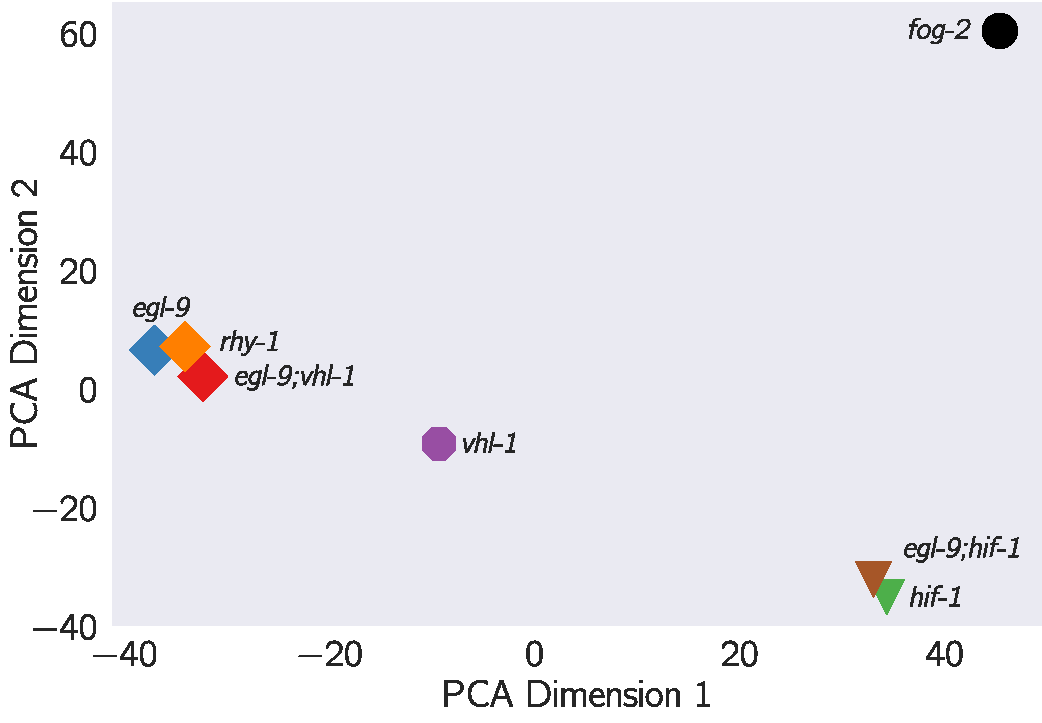
\includegraphics[width=0.5\linewidth]{hypims/pca.pdf}
\caption{
Principal component analysis of various \cel{} mutants. Genotypes that have an
activated hypoxia response (\emph{i.e}, \egl{}, \vhl{}, and \rhy{}) cluster far
from \hif{}. \hif{} clusters with the suppressed \eglhif{} double mutant.
The \fog{} transcriptome, used as an outgroup, is far away from either cluster.
}
\label{fig:pca}
\end{figure}

\subsection*{Reconstruction of the hypoxia pathway from first genetic principles}
\label{sec:reconstruct}
Having shown that the signal in the mutants we selected was sufficient to
cluster mutants using the values of the regression coefficients $\beta$, we set
out to reconstruct the hypoxia pathway from genetic first principles. In general,
to reconstruct a pathway, we must first assess whether two genes act on the same
phenotype. If they do not act on the same phenotype (the set of commonly differentially
regulated genes between two mutants is empty), these mutants are independent.
If they are not independent, then two mutants have a shared transcriptomic
phenotype (STP)---a set of genes or isoforms that are differentially expressed in
both mutants, without taking into account what direction they change in. In this
case, we must measure whether these genes act additively or epistatically on the
measured phenotype; if there is epistasis we must measure whether it is
positive or negative, in order to assess whether the epistatic relationship is a
genetic suppression or a synthetic interaction.

\subsubsection*{Genes in the hypoxia mutant act on the same transcriptional phenotype}
\label{sec:phenotypes}
We observed that all the hypoxia mutants had significant shared transcriptomic
phenotypes (fraction of the transcriptomes that was shared between mutants
ranged from a minimum of 6.8\% shared between \hif{} and \eglvhl{} to a maximum
of 31\% shared genes between \egl{} and \eglvhl{}). For comparison, we also
analyzed a previously published \fog{} transcriptome~\citep{Angeles-Albores2016a}.
The \gene{fog-2} gene is involved in masculinization of the \cel{} germline,
which enables sperm formation, and is not known to be involved in the hypoxia
pathway. The hypoxia pathway mutants and the \fog{} mutant also showed shared
transcriptomic phenotypes (3.6\%--12\% genes), but correlations between
expression level changes were considerably weaker (see below), suggesting that
there is minor cross-talk between these pathways.


% genetic correlations
\begin{figure}[tbhp]
\centering
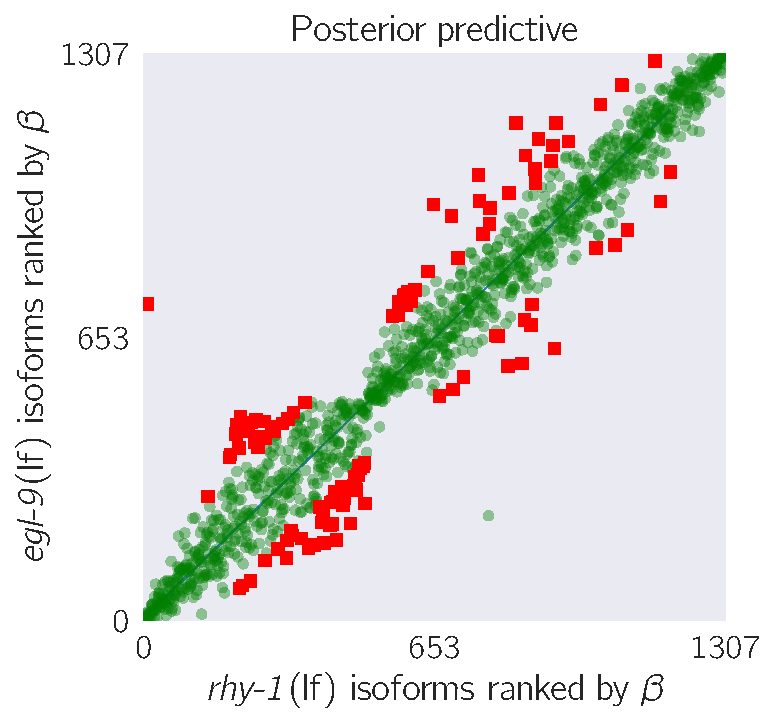
\includegraphics[width=.4\linewidth]{hypims/multiplemodes-eb.pdf}
\caption{
Strong transcriptional correlations can be identified between genes
that share a positive regulatory connection. We took the \egl{} and the \rhy{}
transcriptomes, identified differentially expressed genes common to both
transcriptomes and ranked each gene according to its differential expression
coefficient $\beta$. We plotted the rank of each gene in \rhy{} versus the
rank of the same gene in the \egl{} transcriptome. The result is an almost
perfect correlation. Green, transparent large points mark inliers to the primary
regressions (blue lines); red squares mark outliers to the primary regressions.
}
\label{fig:genetic_interactions}
\end{figure}

We wanted to know whether it was informative to look at quantitative agreement
within STPs. For each mutant pair, we rank-transformed
the regression coefficients $\beta$ of each isoform within the STP, and
calculated lines of best fit using Bayesian regression with a Student-T
distribution to mitigate noise from outliers and plotted the results in a rank plot
(see Fig~\ref{fig:genetic_interactions}). For transcriptomes associated with the
hypoxia pathway, we found that these correlations tended to have
values higher than 0.9 with a tight distribution around the line of best fit.
The correlations for mutants from the hypoxia pathway
with the \fog{} mutant were considerably weaker, with magnitudes between
0.6--0.85 and greater variance around the line of best fit.
Although \gene{hif-1} is known to be genetically repressed by \gene{egl-9}, \gene{rhy-1} and
\gene{vhl-1}~\citep{Epstein2001,Shen2006}, all the correlations
between mutants of these genes and \hif{} were positive.

After we calculated the pairwise correlation within each STP,
we weighted the result of each regression by the
number of isoforms within the STP and
divided by the total number of differentially expressed isoforms present in the
two mutant transcriptomes that contributed to that specific STP,
$N_\mathrm{overlap}/N_{\mathrm{g_1} \cup \mathrm{g2}}$.
The weighted regressions recapitulated a module network (see Fig.~\ref{fig:heatmap}).
We identified a strong positive interaction between \egl{} and \rhy{}.
The magnitude of this weighted correlation derives from the magnitude of the
transcriptomes for these mutants (\egln{} and \rhyn{} differentially expressed
genes respectively) and the overlap between both genes was
extensive, which makes the weighting factor considerably larger than other pairs.
The weak correlation between \hif{} and \egl{} results from the small size of
the \hif{} transcriptome and the small overlap between the transcriptomes.

The fine-grained nature of transcriptional phenotypes means that these weighted
correlations between transcriptomes of single mutants are predictive of genetic
interaction.

% heatmap
\begin{figure}[tbhp]
\centering
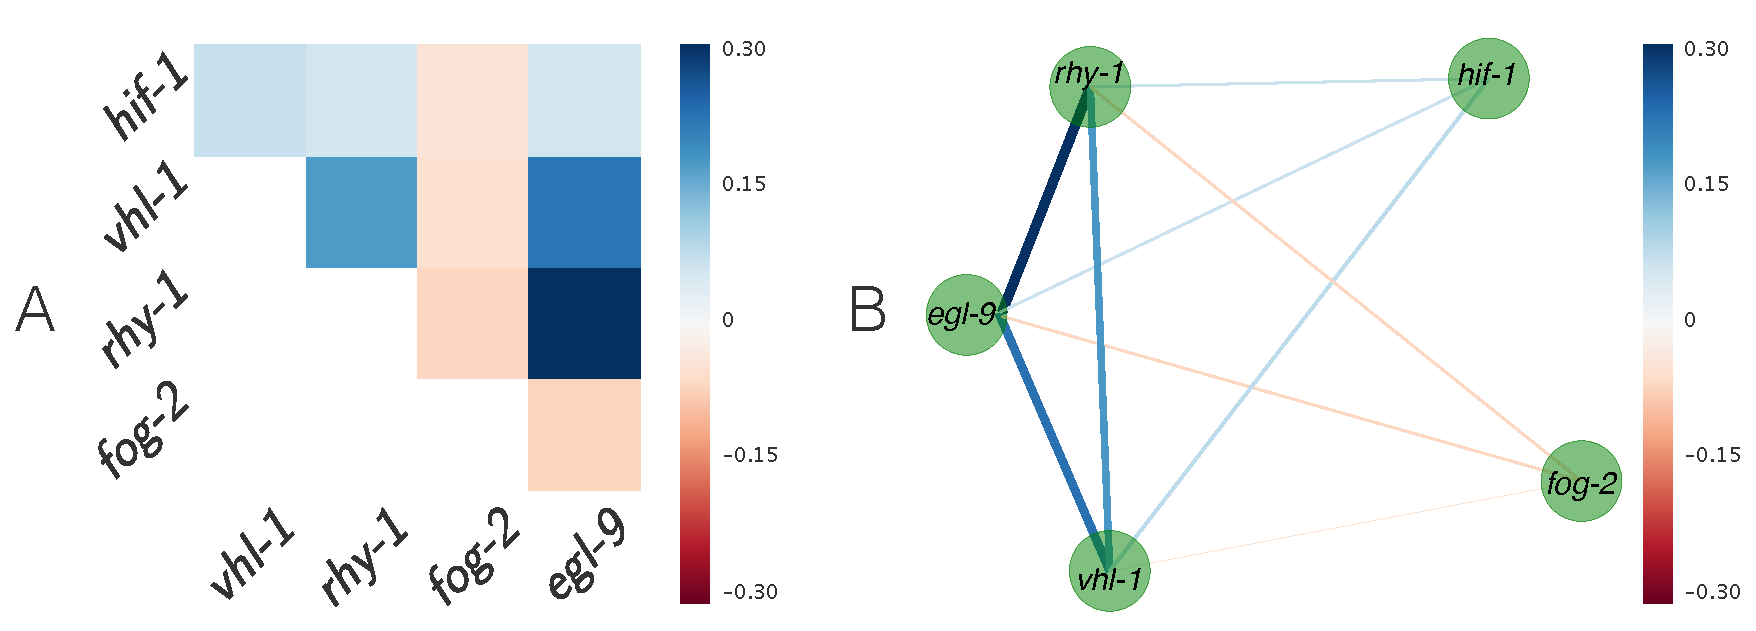
\includegraphics[width=\linewidth]{hypims/bayesian-heatmap-horizontal.pdf}
\caption{
\textbf{A}. Heatmap showing pairwise regression values between all
single mutants. \textbf{B}. Correlation network drawn from \textbf{A}. Edge
width is proportional to the logarithm of the magnitude of the weighted
correlation between two nodes divided by absolute value of the weighted
correlation value of smallest magnitude. Edges are also colored according to the
heatmap in \textbf{A}. Inhibitors of \gene{hif-1} are tightly correlated and form
a control module;
\gene{hif-1} is positively correlated to its inhibitors, albeit weakly;
and
\gene{fog-2}, a gene that is not reported to interact with the hypoxia pathway,
has the smallest, negative correlation to any gene.
}
\label{fig:heatmap}
\end{figure}

\subsubsection*{A quality check of the transcriptomic data reveals excellent agreement
            with the literature}
\label{sub:quality_check}
One way to establish whether genes are acting additively or epistatically to each
other is to perform qPCR of a reporter gene in the single and double mutants. This
approach was used to successfully map the relationships within the hypoxia
pathway (see, for example~\citep{Shao2009,Shen2006}). A commonly used hypoxia reporter
gene is \nhr{}, which is known to exhibit a several-fold increase in mRNA
expression when \hifp{} accumulates~\citep{Shen2006,Shen2005,Park2012}. Likewise,
increased \hifp{} fucntion is known to cause increased of \gene{rhy-1}
and \gene{egl-9}~\citep{Powell-Coffman2010}.

We can
selectively look at the expression of a few genes at a time. Therefore, we
queried the changes in expression of \gene{rhy-1}, \gene{egl-9}, and \nhr{}. We
included the nuclear laminin gene \lam{} as a representative negative control not
believed to be responsive to alterations in the hypoxia pathway.
\nhr{} was upregulated in \egl{}, \rhy{} and \vhl{}, but remains unchanged in \hif{}.
\eglvhl{} had an expression level similar to \egl{}; whereas the
\eglhif{} mutant showed wild-type levels of the reporter expression, as reported
previously~\citep{Shen2006} (see Fig.~\ref{fig:qpcr}).

% in silico qPCR
\begin{figure}[tbhp]
\centering
\includegraphics[width=.5\linewidth]{hypims/qpcr.pdf}
\caption{
\textbf{Top}: Observed $\beta$ values of select genes. We selected
four genes (\gene{rhy-1}, \gene{egl-9}, \nhr{} and \lam{}, shown on the x-axis)
and plotted their regression coefficients, $\beta$, as measured for every
genotype (represented by one of six colors) to study the epistatic relationships
between each gene. Asterisks above a bar represent a regression coefficient
statistically significantly different from 0 (\qval{1}) relative to a wild-type
control. Error bars show standard error of the mean
value of $\beta$. \nhr{} is an expression reporter that has been used previously
to identify \gene{hif-1} regulators~\citep{Shen2006,Shao2009}. \lam{} is shown here
as a negative control that should not be altered by mutations in this pathway.
We measured modest increases in the levels of \gene{rhy-1} mRNA when \hif{} is
knocked out.
}
\label{fig:qpcr}
\end{figure}

We observed changes in \rhy{} expression consistent with previous
literature~\citep{Shen2006} when \hifp{} accumulates.
We also observed increases in \gene{egl-9} expression in \egl{}.
\gene{egl-9} is known as a hypoxia responsive gene~\citep{Powell-Coffman2010}.
Although changes in \gene{egl-9} expression were not statistically significantly
different from the wild-type in
\rhy{} and \vhl{} mutants, the mRNA levels of \gene{egl-9} still trended towards
increased expression in these genotypes.
As with \nhr{}, \gene{egl-9} and \gene{rhy-1} expression were wild-type in
\eglhif{} and \eglvhl{} mutant showed expression phenotypes identical to \egl{}.
This dataset also showed that knockout of \gene{hif-1} resulted in a modest
increase in the levels of \gene{rhy-1}. This suggests that \gene{hif-1}, in
addition to being a positive regulator of \gene{rhy-1}, also inhibits it, which
constitutes a novel observation.
Using a single reporter we would have been able to reconstruct an
important fraction of the genetic relationships between the genes in the hypoxia
pathway–--but would likely fail to observe yet other genetic interactions, such as
the evidence for \gene{hif-1} negatively regulating \gene{rhy-1} transcript levels.


\subsection*{Transcriptome-wide epistasis}
Ideally, any measurement of transcriptome-wide epistasis should conform to certain
expectations. First, it should make use of the regression coefficients of as
many genes as possible. Second, it should be summarizable in a single,
well-defined number. Third, it should have an intuitive behavior, such that
special values of the statistic should each have an unambiguous interpretation.

One way of displaying transcriptome-wide epistasis is to plot transcriptome data onto
an epistasis plot (see Fig~\ref{fig:egl9epistasis}). In an epistasis plot, the
X-axis represents the expected expression of a double mutant $a^-b^-$ if $a$
and $b$ interact additively.
In other words, each individual isoform's x-coordinate is the sum of the regression
coefficients from the single mutants $a^-$ and $b^-$.
The Y-axis represents the deviations from the additive (null) model, and
can be calculated as the difference between the observed regression coefficient
and the predicted regression coefficient. Only genes that are differentially
expressed in all three genotypes are plotted. Assuming that the two genes interact
via a simple phenotype (for example, if both genes affect a transcription factor
that generates the entire transcriptome), these plots will generate specific
patterns that can be described through linear regressions. The slope of these
lines, $s_{a,b}$, is the transcriptome-wide epistasis coefficient.

Epistasis plots can be understood intuitively for simple cases of genetic
interactions. If two genes act additively on the same set of differentially expressed
isoforms then all the plotted points will fall along the line $y=0$.
If two genes interact in an unbranched pathway, then $a^-$ and $b^-$ should
have identical phenotypes for $a^-$, $b^-$ and $a^-b^-$, if all the genotypes are
homozygous for genetic null alleles~\citep{Huang2006}. It follows that the
data points should fall along a line with slope equal to $-\frac{1}{2}$. On the
other hand, in the limit of complete inhibition of $a$ by $b$, the plots should show
a line of best fit with slope equal to $-1$\footnote{Specifically, this follows
from assuming that $b^-$ is wild-type under the conditions assayed; and
$a^-b^-$ = $b^-$ = wild-type}.
Genes that interact synthetically (\emph{i.e.}, through an OR-gate) will fall
along lines with slopes $>0$. When there is epistasis of one gene over another,
the points will fall along a line of best fit with slope $s_{ab=b}$ or $s_{ab=a}$.
This slope must be determined from the single-mutant data.
From this information, we can use the single mutant data to predict the
distribution of slopes that results for each case stated above, as well as for
each epistatic combination ($a^-b^-=a^-$ or $a^-b^-=b^-$). The transcriptome-wide
epistasis coefficient ($s_{a, b}$), emerges as a powerful way to quantify epistasis
because it integrates information from many different genes or isoforms into a
single number (see Fig.~\ref{fig:egl9epistasis}).

In our experiment, we studied two double mutants, \eglhif{} and \eglvhl{}.
We wanted to understand how well an epistasis analysis based on transcriptome-wide
coefficients agreed with the epistasis results reported in the literature, which
were based on qPCR of single genes. Therefore, we performed orthogonal distance
regression on the two gene combinations we studied (\gene{egl-9} and
\gene{vhl-1}; and \gene{egl-9} and \gene{hif-1}) to determine the epistasis
coefficient for each gene pair. We also generated models for the special cases
mentioned above (additivity, $a^-b^-=a^-$, strong suppression, etc\ldots) using
the single mutant data. For every simulation, as well as for the observed data,
we used bootstraps to generate probability distributions of the epistasis
coefficients.

When we compared the predictions for the transcriptome-wide epistasis coefficient,
$s_{egl-9,vhl-1}$ under different assumptions with the observed slope ($-0.42$). We
observed that the predicted slope matched the simulated slope for the case where
\gene{egl-9} is epistatic over \gene{vhl-1} (\egl{} = \eglvhl{}, see
Fig.~\ref{fig:egl9epistasis}) and did not overlap with any other prediction.
Next, we predicted the distribution of $s_{egl-9,hif-1}$ for different pathways
and contrasted with the observed slope. In this case, we saw that the uncertainty
in the observed coefficient overlapped significantly with the strong suppression
model, where \eglp{} strongly suppresses \hifp{}, and also with the model where
\hif{} = \eglhif{}. In this case, both models are reasonable---\hifp{} is strongly
suppressed by \eglp{}, and we know from previous literature that the epistatic
relationship, \hif{} = \eglhif{}, is true for these mutants. In fact, as the
repression of \hifp{} by \eglp{} becomes stronger, the epistatic model should converge
on the limit of strong repression (see
\href{https://wormlabcaltech.github.io/mprsq/analysis_notebooks/epistasis_6.html}
{Epistasis}).

Another way to test which model best explains the epistatic relationship between
\gene{egl-9} and \gene{vhl-1} is to use Bayesian model selection to calculate
an odds ratio between two models to explain the observed data. Models can be placed
into two categories: parameter-free and fit. Parameter free models are `simpler'
because their parameter space is smaller (0 parameters) than the fit models ($n$
parameters). By Occam's razor, simpler models should be preferred to more
complicated models. However, simple models suffer from the drawback that
systematic deviations from them cannot be explained or accomodated, whereas more
complicated models can alter the fit values to maximize their explanatory power.
In this sense, more complicated models should be preferred when the data shows
systematic deviations from the simple model. Odds-ratio selection gives us a way
to quantify the trade-off between simplicity and explanatory power.

We reasoned that comparing a fit model ($y = \alpha\cdot x$, where $\alpha$ is
the slope of best fit) against a parameter-free model ($y = \gamma\cdot x$,
where $\gamma$ is a single number) constituted a conservative approach towards
selecting which theoretical model (if any) best explained the data. In particular,
this approach will tend to strongly favor the line of best fit over simpler model
for all but very small, non-systematic deviations. We decided
that we would reject the theoretical models only if the line of best-fit
was $10^3$ times more likely than the theoretical models (odds ratio, OR $>10^3$).
Comparing the odds-ratio between the line of best fit and the different pathway
models for \gene{egl-9} and \gene{vhl-1} showed similar results to the simulation.
Only the theoretical model \egl{} = \eglvhl{} could not be rejected (OR = 0.46),
whereas all other models were significantly less likely than the line of best fit
(OR $>10^{44}$).
Therefore, \gene{egl-9} is epistatic to \gene{vhl-1}. Moreover,
since $s_{egl-9, vhl-1}$ is strictly between and not equal to $0$ and $-0.5$, we
conclude that \gene{egl-9} acts on its transcriptomic phenotype in
\gene{vhl-1}-dependent and independent manners. A branched pathway that can lead
to epistasis coefficients in this range is a pathway where \gene{egl-9} interacts
with its transcriptomic phenotype via branches that have the same valence (both
positive or both negative)~\citep{Shao2009}. When we performed a similar analysis
to establish the epistatic relationship between \gene{egl-9} and \gene{hif-1},
we observed that the best alternative to a free-fit model was a model where
\gene{hif-1} is epistatic over \gene{egl-9} (OR$=2551$), but the free-fit model
was still preferred. All other models were strongly rejected (OR $>10^{25}$).

% epistasis graph
\begin{figure}[tbhp]
\centering
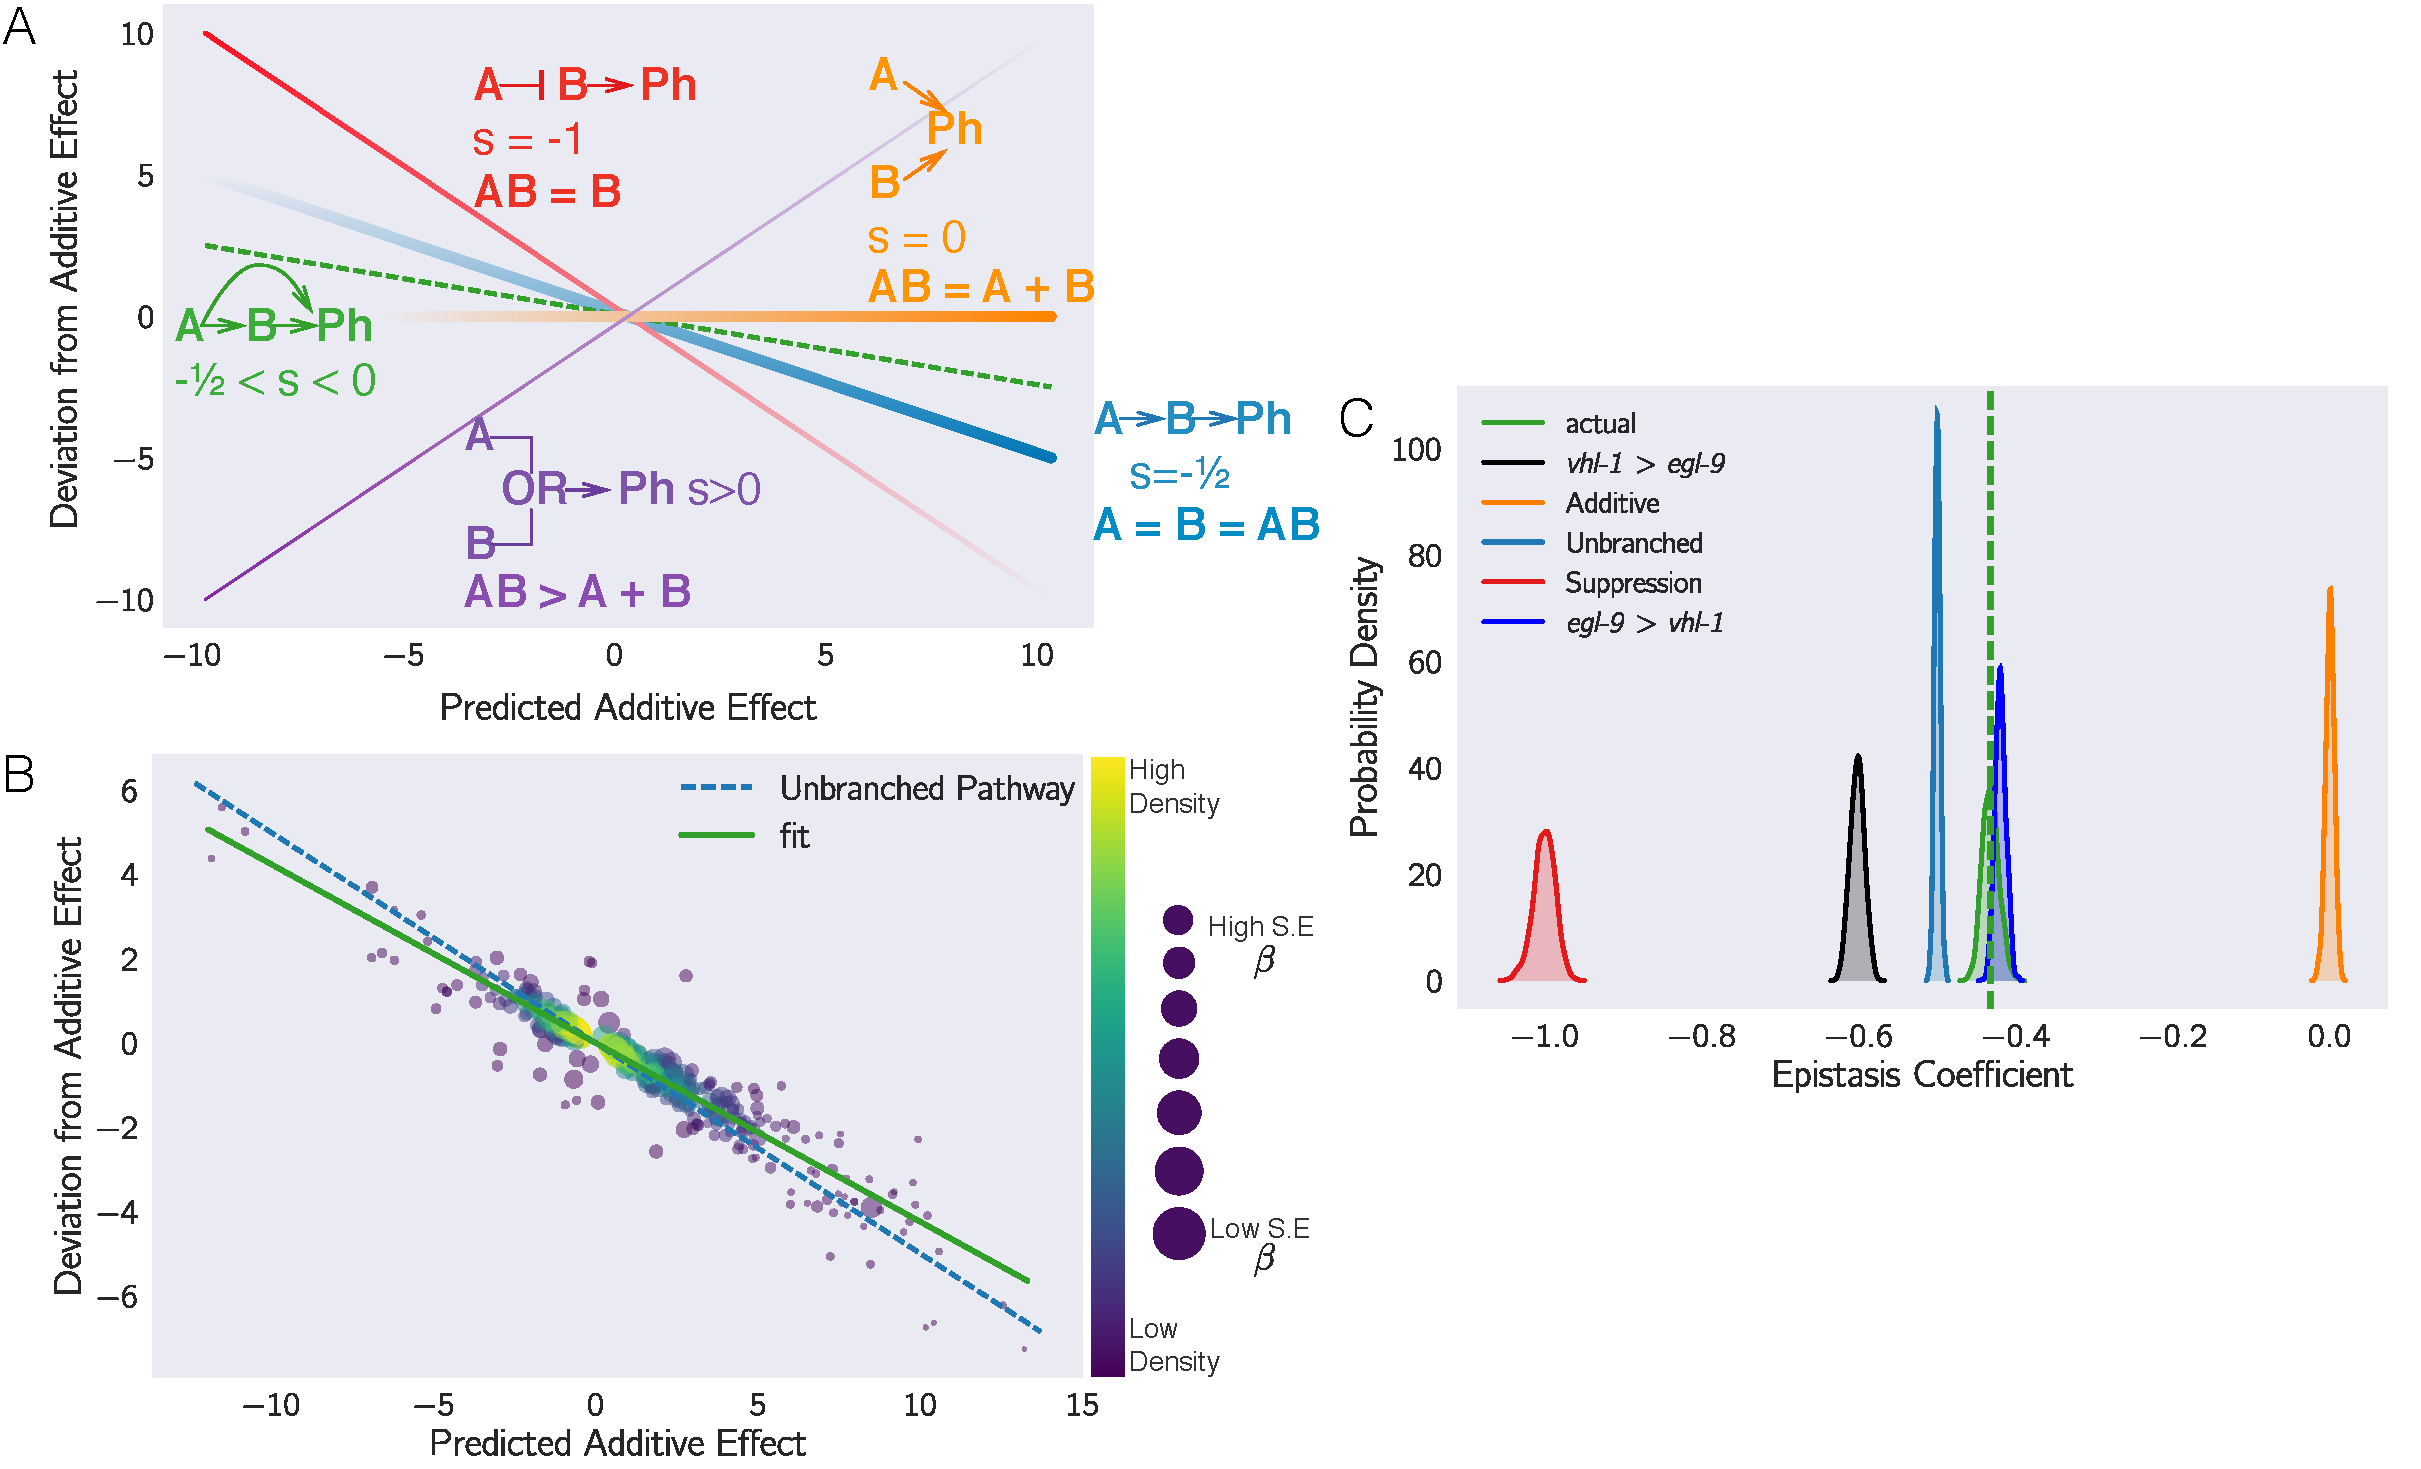
\includegraphics[width=\linewidth]{hypims/egl9hif1-epistasis-horizontal.pdf}
\caption{
(\textbf{A}) Schematic diagram of an epistasis plot. The X-axis on an epistasis
plot is the expected coefficient for a double mutant under an additive model
(null model). The Y-axis plots deviations from this model. Double mutants that
deviate in a systematic manner from the null model exhibit transcriptome-wide epistasis
($s$). To measure $s$, we perform a linear regression on the data. The slope of
the line of best fit is $s$. This coefficient is related to genetic architectures.
Genes that act additively on a phenotype \textbf{(Ph)} will have $s=0$ (orange
line); whereas
genes that act along an unbranched pathway will have $s=-1/2$ (blue line).
Strong
repression is reflected by $s=-1$ (red line). Cases where $s>0$ correspond to
synthetic interactions (purple line), and in the limit as $s\rightarrow\infty$,
the synthetic interaction
must be an OR-gate. Cases where $0 < s < -1/2$ correspond to circuits
that have multiple positive branches; whereas cases where
$-1/2<s< -1$ correspond to cases where the branches have different valence.
Cases where $s < -1$ represent inhibitory branches.
(\textbf{B}) Epistasis plot showing
that the \eglvhl{} transcriptome deviates significantly from a null additive.
Points are colored qualitatively according to density (purple---low,
yellow---high) and size is inversely proportional to the standard
error (S.E.) of the y-axis (larger points, higher accuracy). The purple line
is the line of best fit from an orthogonal distance regression.
(\textbf{C}) Comparison of simulated epistatic coefficients against the observed
coefficient. Green curve shows the bootstrapped observed transcriptome-wide epistasis
coefficient for \gene{egl-9} and \gene{vhl-1}. Dashed green line shows the mean
value of the data. Using the single mutants, we simulated coefficient
distributions for a linear model (light blue, centered at $-0.5$);
an additive model (orange, centered at 0); a model where either
\gene{egl-9} or \gene{vhl-1} masks the other phenotype (dark blue and black,
respectively) and a complete suppression model (red, centered at $-1$).
The observed coefficient overlaps the predicted epistasis curve for
\eglvhl{} = \egl{} (green and dark blue).
}
\label{fig:egl9epistasis}
\end{figure}

\subsubsection*{Epistasis can be predicted}
Given our success in measuring epistasis coefficients, we wanted to know whether
we could predict the epistasis coefficient between \gene{egl-9} and \gene{vhl-1}
in the absence of the \egl{} genotype. Since \rhyp{} indirectly activates
\eglp{}, the \rhy{} transcriptome should contain more or less
equivalent information to the \egl{} transcriptome. Therefore, we generated
predictions of the epistasis coefficient between \gene{egl-9} and \gene{vhl-1}
by substituting in the \rhy{} data. We predicted $s_{rhy-1,vhl-1} = -0.45$.
Similarly, we used the \eglvhl{} double mutant to
measure the epistasis coefficient while replacing the \egl{} dataset with the \rhy{}
dataset. We found that the epistasis coefficient using this substitution was $-0.40$.
This coefficient was different from $-0.50$ (OR $>10^{62}$), reflecting the same
qualitative conclusion that the hypoxia pathway is branched.
In conclusion, we were able to obtain a quantitatively close prediction of the
epistasis coefficient for two mutants using the transcriptome of a related,
upstream mutant. Finally, we showed that in the absence of a single mutant, an
upstream locus can under some circumstances be used to estimate epistasis
between two genes.


\subsection*{Transcriptomic decorrelation can be used to infer functional distance}
\label{sub:decorrelation}
% What are functional interactions?
So far, we have shown that RNA-seq can accurately measure genetic interactions.
However, genetic interactions are far removed from biochemical interactions:
Genetic interactions do not require two gene products to interact physically, nor
even to be physically close to each other. RNA-seq cannot measure physical
interactions between genes, but we wondered whether expression profiling contains
sufficient information to order genes along a pathway.

Single
genes are often regulated by multiple independent sources. The connection between
two nodes can in theory be characterized by the strength of the edges connecting
them (the thickness of the edge); the sources that regulate both
nodes (the fraction of inputs common to both nodes); and the genes that are
regulated by both nodes (the fraction of outputs that are common to both nodes).
In other words, we expected that expression profiles associated with a pathway
would respond quantitatively to quantitative changes in activity of the pathway.
Targeting a pathway at multiple points would lead to expression profile
divergence as we compare nodes that are separated by more degrees of freedom,
reflecting the flux in information between them.

% decorrelation
\begin{figure}[tbhp]
\centering
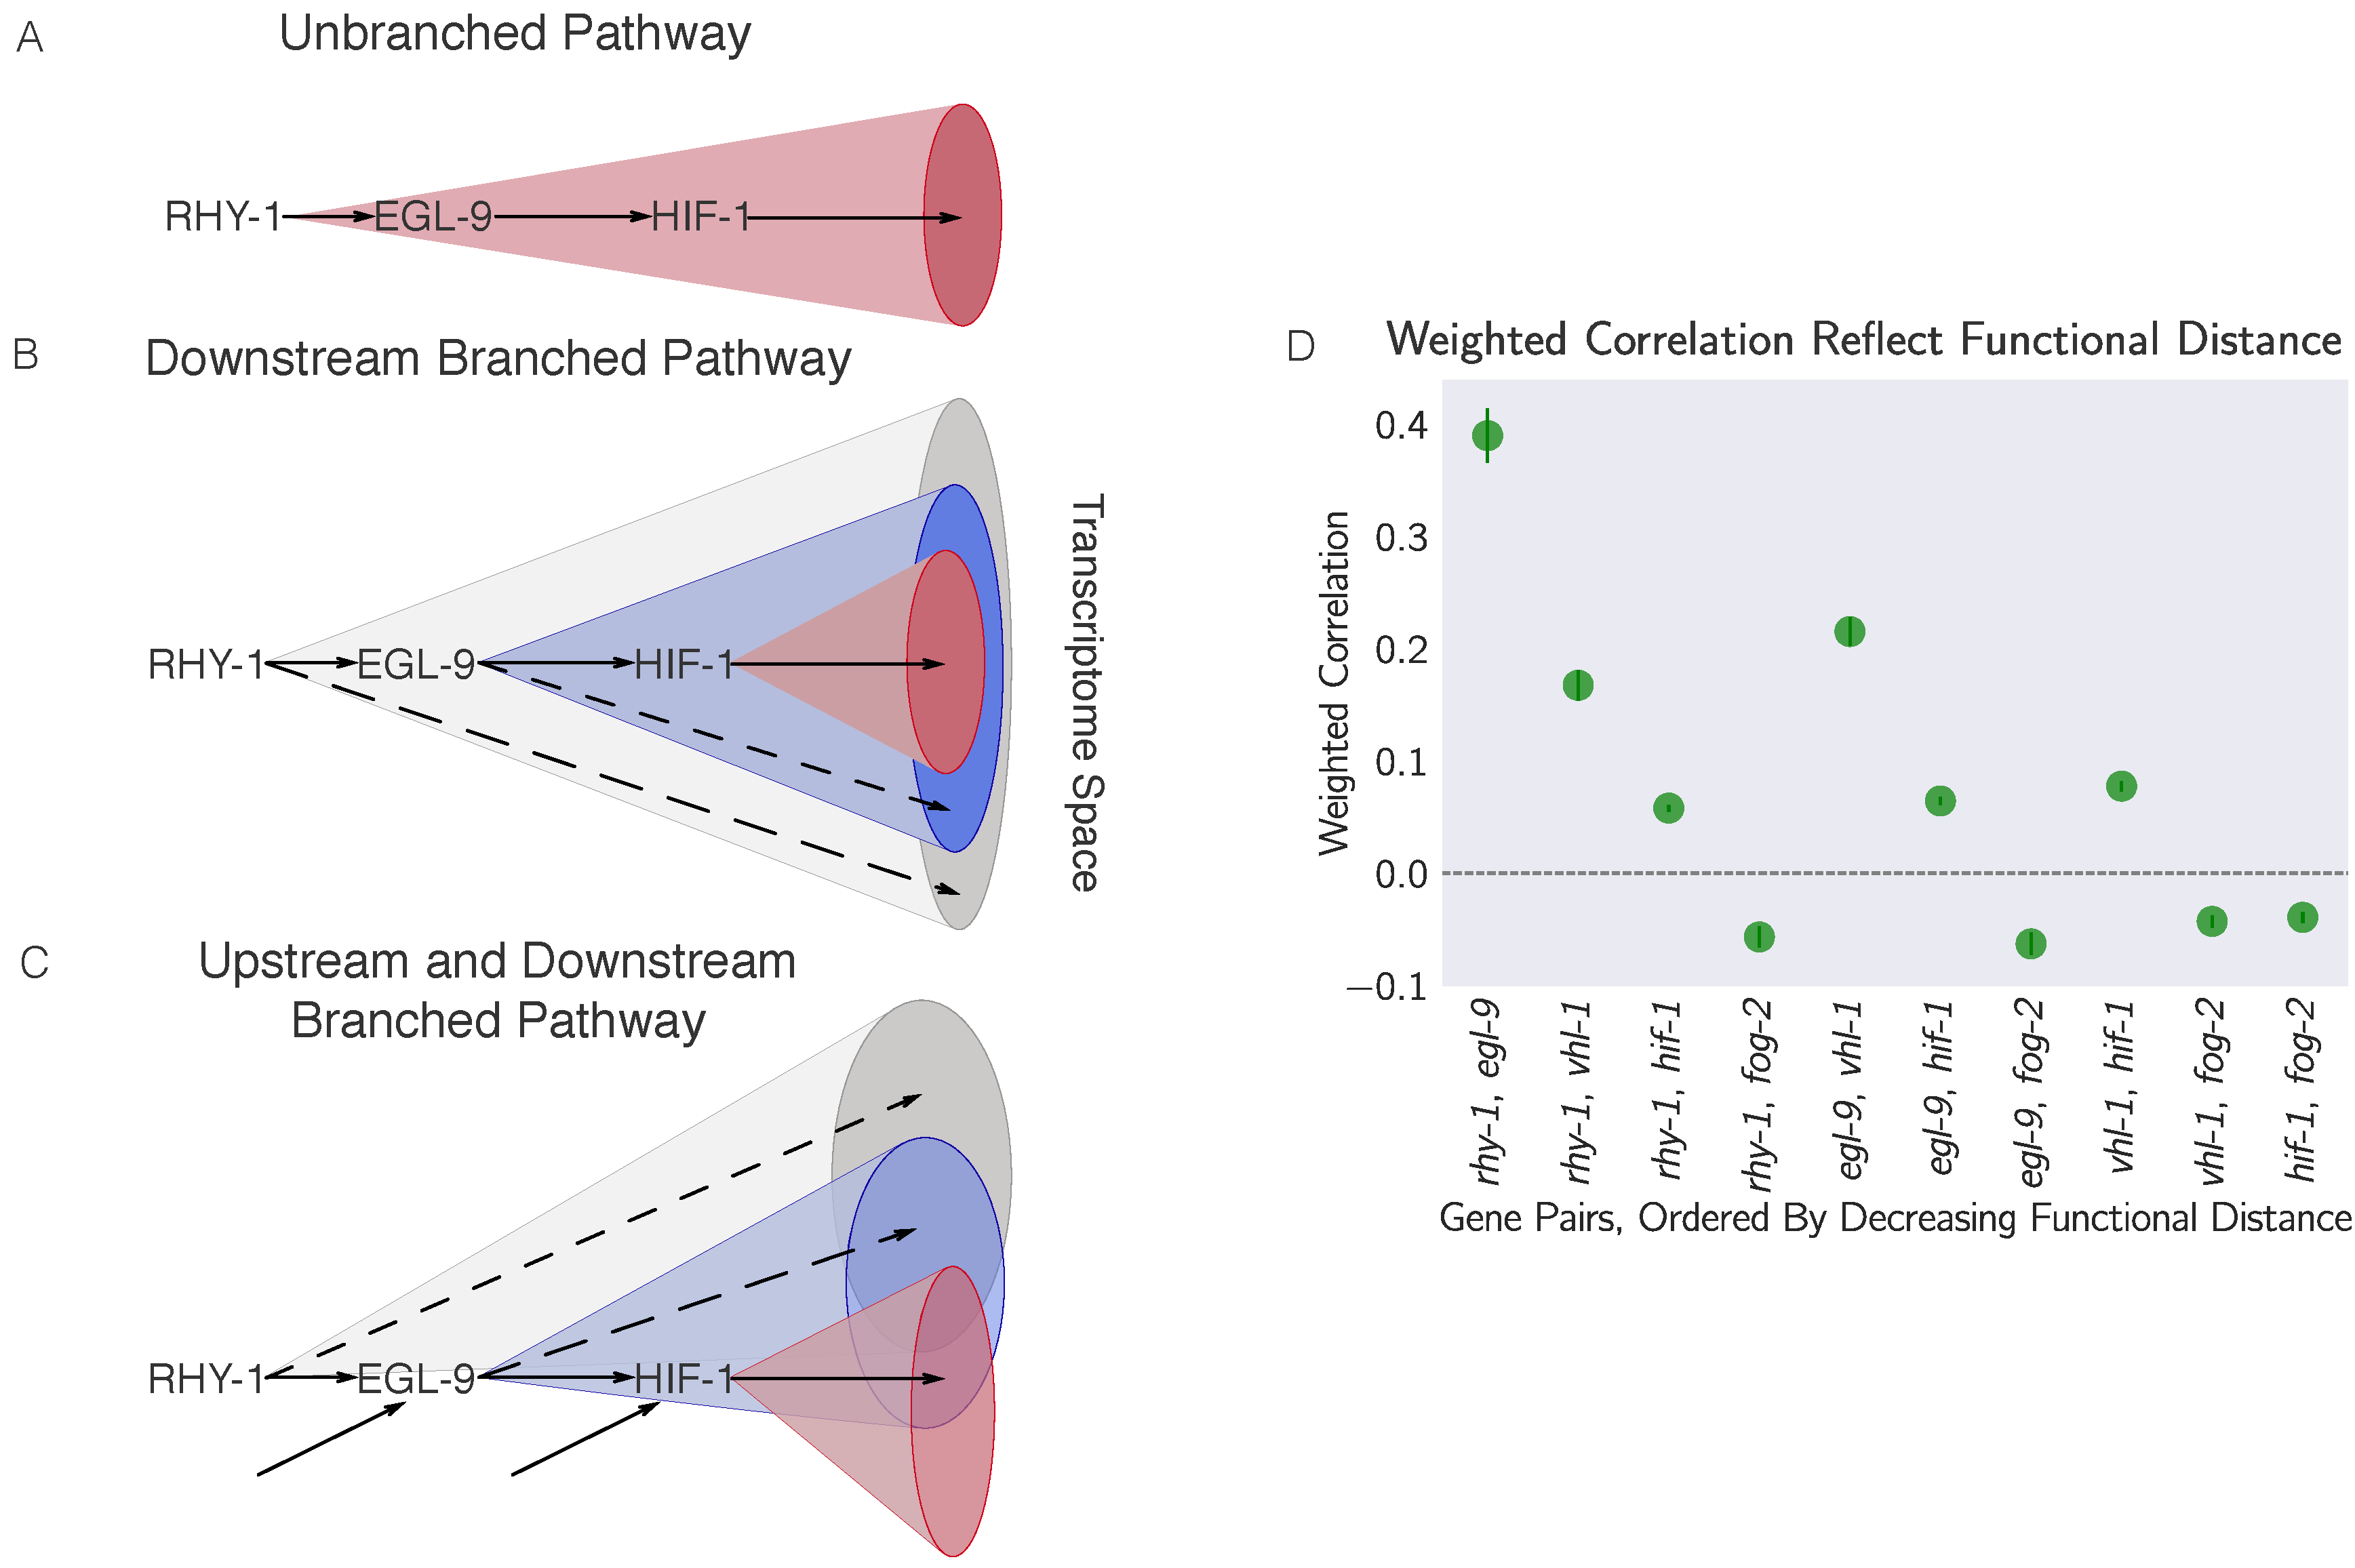
\includegraphics[width=.8\linewidth]{hypims/decorrelation-horizontal.pdf}
\caption{
Theoretically, transcriptomes can be used to order genes in a pathway under
certain assumptions. Arrows in the diagrams above are intended to show the
direction of flow, and do not indicate valence.
\textbf{A}. A linear pathway in which \gene{rhy-1} is the only gene controlling
\gene{egl-9}, which in turn controls \gene{hif-1} does not contain information
to infer the order between genes.
\textbf{B}. If \gene{rhy-1} and \gene{egl-9} have transcriptomic effects that are
separable from \gene{hif-1}, then the \gene{rhy-1} transcriptome should contain
contributions from \gene{egl-9}, \gene{hif-1} and \gene{egl-9}- and
\gene{hif-1}-independent pathways. This pathway contains enough information to
infer order.
\textbf{C}. If a pathway is branched both upstream and downstream,
transcriptomes will show even faster decorrelation. Nodes that are
separated by many edges may begin to behave almost independently of each other
with marginal transcriptomic overlap or correlation.
\textbf{D}. The hypoxia pathway can be ordered.
We hypothesize the rapid decay in correlation is due to a mixture of
upstream and downstream branching that happens along this pathway. Bars show the
standard error of the weighted coefficient from the Monte Carlo Markov Chain
computations.
}
\label{fig:decorrelation}
\end{figure}


We investigated the possibility that transcriptomic signals do in fact contain
relevant information about the degrees of separation by weighting the robust
Bayesian regression between each pair of genotypes by the size of the shared
transcriptomic phenotype of each pair divided by the total number of isoforms
differentially expressed in either mutant
($N_\mathrm{Intersection}/N_{\mathrm{Union}}$). We plotted the weighted
correlation of each gene pair, ordered by increasing functional distance
(see Fig.~\ref{fig:decorrelation}). In every case, we see that the weighted
correlation decreases monotonically due mainly, but not exclusively, to a smaller
STP.\@ We believe that this result is not due to random noise or insufficiently
deep sequencing. Instead, we propose a framework in which every gene is regulated
by multiple different molecular species, which induces progressive decorrelation.
This decorrelation in turn has two consequences. First, decorrelation within a
pathway implies that two nodes may be almost independent of each other if the
functional distance between them is large. Second, it may be possible to use
decorrelation dynamics to infer gene order in a branching pathway, as we have
done with the hypoxia pathway.

\subsection*{The circuit topology of the hypoxia pathway explains patterns in
            the data}
\label{sub:topology}
We noticed that while some of the rank plots contained a clear positive correlation
(see Fig.~\ref{fig:genetic_interactions}), other rank plots showed
a discernible cross-pattern (see Fig.~\ref{fig:xpattern}). In particular, this
cross-pattern emerged between \vhl{} and \rhy{} or between \vhl{} and \egl{},
even though genetically \gene{vhl-1}, \gene{rhy-1} and \gene{egl-9} are all
inhibitors of \hif{}. Such cross-patterns could be indicative of feedback loops
or other complex interaction patterns.

% correlative genetics again
\begin{figure}[tbhp]
\centering
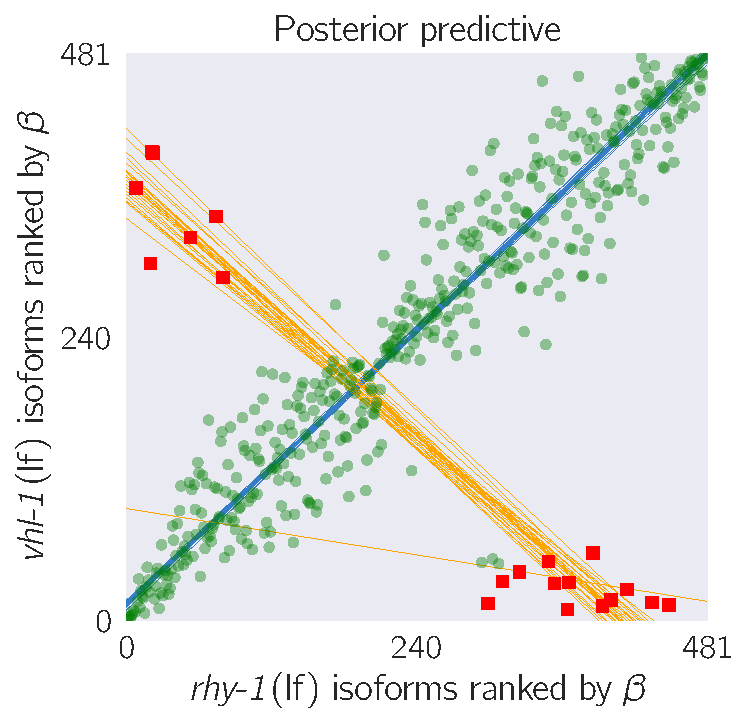
\includegraphics[width=.4\linewidth]{hypims/multiplemodes-ed.pdf}
\caption{
A feedback loop can generate transcriptomes that are both
correlated and anti-correlated. The \vhl{}/\rhy{} STP shows a cross-pattern.
Green large points are inliers to the first
regression. Red squares are outliers to the first regression. Only the red
small points were used for the secondary regression. Blue lines are representative
samples of the primary bootstrapped regression lines. Orange lines are
representative samples of the secondary bootstrapped regression lines.
}
\label{fig:xpattern}
\end{figure}



If the above is correct, then it should be possible to identify
\gene{egl-9}-independent, \rhy{}-dependent target genes in a
logically consistent way.
One erroneous way to identify these targets is via
subtractive logic. Using subtractive logic, we would identify genes that are
differentially expressed in \rhy{} mutants but not in \egl{} mutants.  Such a
gene set would
consist of almost 700 genes. One major drawback of subtractive logic is that it
cannot be applied when feedback loops exist between the genes in question.
Another problem is that the set of identified genes are statistically indistinguishable
from false positive and false negative hits because they have no distinguishing
property beyond the condition that they should be differentially expressed in
one mutant but not the other. In fact, this is exactly the behavior expected of
false-positive or false-negative hits---presence in one, but not multiple, mutants.
We need to consider the relationship between two genes before we can begin to
identify targets which expression is dependent on one gene and independent
of the other.

\gene{rhy-1} and \gene{egl-9} share a well-defined relationship. \rhyp{}
inhibits \cyslp{},
which in turn inhibits \eglp{}~\citep{Ma2012}. Therefore, loss of \rhyp{} leads
to inactivation of \eglp{}, which leads to increase in the cellular levels of
\hifp{}. \hifp{} in turn causes the mRNA levels of \gene{rhy-1} and \gene{egl-9}
to increase,
as they are involved in the \gene{hif-1}-dependent hypoxia response. However, since
\gene{rhy-1} has been mutated, the observed transcriptome is
\rhyp{} `null'; \eglp{} `null'; \hifp{} `on'. The situation is similar for
\egl{}, except that \rhyp{}
is not inactive, and therefore the observed transcriptome is the result of
\rhyp{} `up'; \eglp{} `null'; and \hifp{} `on'. From this pattern, we conclude that
the \egl{} and \rhy{} transcriptomes should exhibit a cross-pattern when plotted
against each other: The positive
arm of the cross is the result of the \eglp{} `null'; \hifp{} `on' dynamics; and the
negative arm reflects the different direction of \rhyp{} activity between
transcriptomes. No negative arm is visible (with the exception of two
outliers, which are annotated as pseudogenes in WormBase). Therefore, in this
dataset we do not find genes that have \gene{egl-9} independent,
\gene{rhy-1}-dependent expression patterns.

We also identified a main hypoxia response induced by disinhibiting
\gene{hif-1} (355 genes) by identifying genes that were commonly up-regulated
amongst \egl{}, \rhy{} and \vhl{} mutants. Although the hypoxic response is likely
to involve between three and seven times more genes (assuming the \rhy{} transcriptome
reflects the maximal hypoxic response), this is a conservative
estimate that minimizes false positive results, since these changes were
identified in four different genotypes with three replicates each. This response
included five transcription factors (\gene{W02D7.6}, \nhr{}, \gene{ztf-18},
\gene{nhr-135} and \gene{dmd-9}). The full list of genes associated with the
hypoxia response can be found in the Supplementary Table 1.
% TODO: SI numbering

\gene{hif-1}-independent effects of \gene{egl-9} have been reported
previously~\citep{Park2012}, which led us to question whether we could identify
similar effects in our dataset. We have observed that \hif{} displays a modest
increase in the transcription of \gene{rhy-1}, from which we speculated that
\eglp{} would have increased activity in the \hif{} mutant compared to the wild-type.
Therefore, we searched for genes that were regulated in an opposite manner between
\hif{} and \eglhif{}, and that were regulated in the same direction between
all \egl{} genotypes. We did not find any genes that met these conditions.

We also searched for genes with \gene{hif-1} independent, \gene{vhl-1}-dependent gene
expression and found \vhltargets{} genes, which can be found in the Supplementary
Table 2.
Finally, we searched for candidates directly regulated by \gene{hif-1}. Initially, we
searched for genes that had were significantly altered in \hif{} genotypes in one
direction, but altered in the opposite direction in mutants that activate the
\hifp{} response. Only two genes (\emph{R08E5.3}, and \emph{nit-1}) met these
conditions. This could reflect the fact that \hifp{} exists at very low
levels in \cel{}, so loss of function mutations in \gene{hif-1} might only have
mild effects on its transcriptional targets. We reasoned that genes
that are overexpressed in mutants that induce the \hifp{} response would be enriched
for genes that are direct candidates.  We found \hiftargets{}  genes which have
consistently increased expression in mutants with a constitutive hypoxic response.
These genes can be found in the Supplementary Table 3.


\subsubsection*{Enrichment analysis of the hypoxia response}
\label{sub:ea_hypoxia}
To validate that our transcriptomes were correct, and to understand how
functionalities may vary between them, we subjected each decoupled response to
enrichment analysis using the WormBase Enrichment Suite~\citep{Angeles-Albores2016,
Angeles-Albores2016b}.

\begin{figure}[tbhp]
\centering
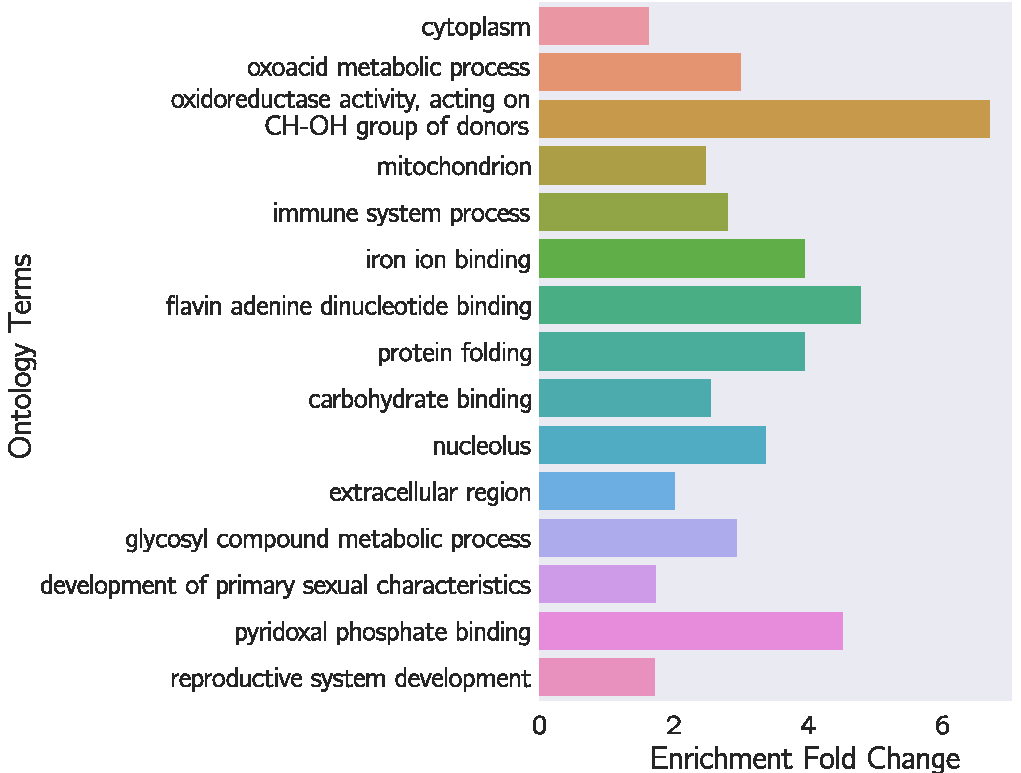
\includegraphics[width=.7\linewidth]{hypims/hypoxia_response_gea.pdf}
\caption{
Gene ontology enrichment analysis of genes associated with the main hypoxia response.
A number of terms reflecting catabolism and bioenergetics are enriched.
}
\label{fig:hyp_gea}
\end{figure}

We used gene ontology enrichment analysis (GEA) on the main hypoxia response program.
This showed that the terms `oxoacid metabolic process' (\qval{4}, 3.0 fold-change,
24 genes), `iron ion binding' (\qval{2}, 3.8 fold-change, 10 genes), and `immune
system process' (\qval{3}, 2.9 fold-change, 20 genes) were significantly enriched.
GEA also showed enrichment of the term `mitochondrion' (\qval{3}, 2.5 fold-change,
29 genes) (see Fig.~\ref{fig:hyp_gea}). Indeed, \hif{} has been implicated in
all of these biological and molecular functions~\citep{Luhachack2012,Ackerman2012,
Romney2011,Semenza2011}.
As benchmark on the quality of our data, we selected a set of 22 genes known to
be responsive to \hifp{} levels from the literature and asked whether these genes
were present in our hypoxia response list. We found $8/22$ known genes, which
constitutes a statistically significant result ($p<10^{10}$). The small number of
reporters found in this list probably reflects the conservative nature of our
estimates.
We studied the \gene{hif-1}-independent, \gene{vhl-1}-dependent gene set
using enrichment analysis but no terms were significantly enriched.

\subsection*{Identification of non-classical epistatic interactions}
\label{sub:hifoh}
\hif{} has traditionally been viewed as existing in a genetic OFF state under
normoxic conditions. However, our dataset indicates that \hifn{} genes show
altered expression when \gene{hif-1} function is removed in normoxic conditions.
Moreover, we observed positive correlations between \hif{} $\beta$ coefficients
and \egl{}, \vhl{} and \rhy{} $\beta$ coefficients in spite of the negative
regulatory relationships between these genes and \gene{hif-1}. Such
positive correlations could indicate a different relationship between these genes
than has previously been reported, so we attempted to substantiate them through
epistasis analyses.

To perform epistasis analyses, we first identified genes that exhibited violations
of the canonical genetic model of the hypoxia pathway. To this end, we searched for
genes that exhibited different behaviors between \egl{} and \vhl{}, or
between \rhy{} and \vhl{} (we assume that all results from the
\rhy{} transcriptome reflect a complete loss of \gene{egl-9} activity). We found
\hifohtargets{} that satisfied this condition (see Fig.~\ref{fig:hif1oh},
Supplemental Table 4).
Additionally, many of these genes exhibited a new kind of epistasis. Namely,
\gene{egl-9} was epistatic over \gene{vhl-1}. Identification of a set of genes
that have a consistent set of relationships between themselves suggests that
we have identified a new aspect of the hypoxia pathway.

\begin{figure}[tbhp]
\centering
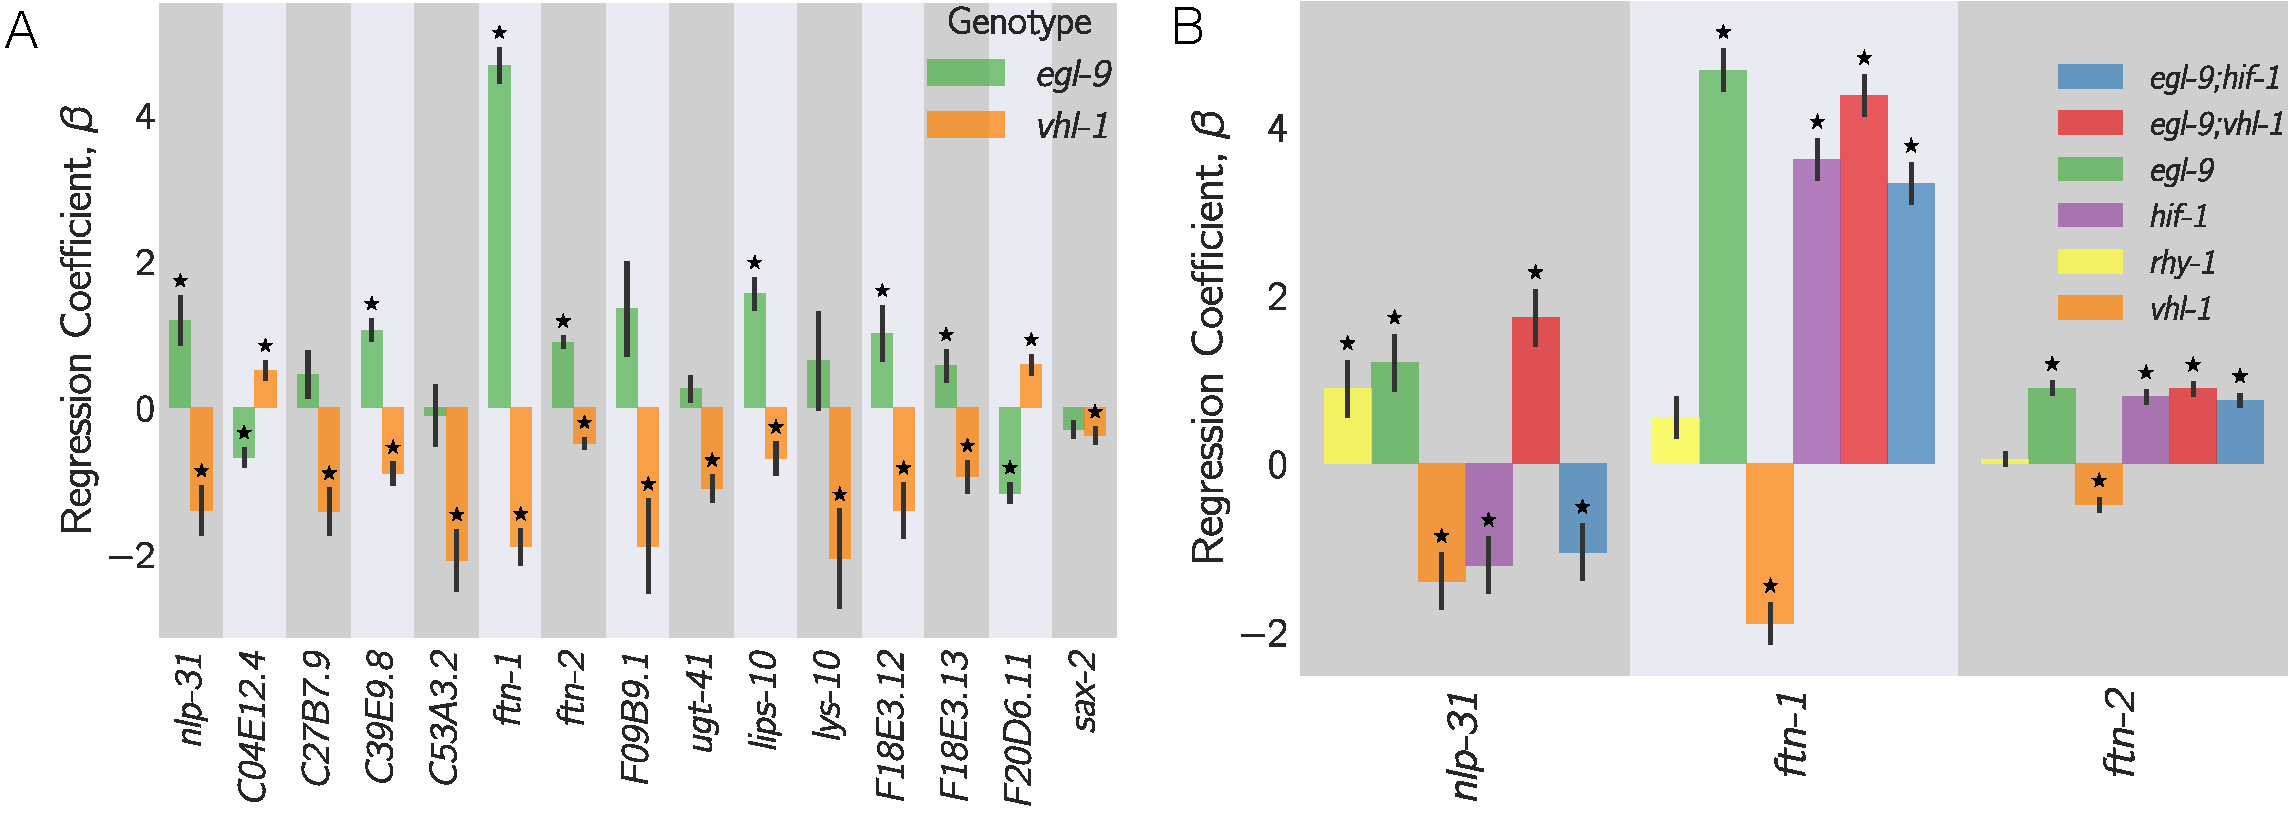
\includegraphics[width=\linewidth]{hypims/hif1oh-epistasis-horizontal.pdf}
\caption{
\textbf{A}. 27 genes in \cel{} exhibit non-classical epistasis in the hypoxia
pathway, characterized by opposite effects on gene expression, relative to the
wild-type, of of the \vhl{} compared to \egl{} (or
\rhy{}) mutants. Shown are a random selection of 15 the 27 genes for illustrative
purposes.
\textbf{B}. Representative genes showing that non-canonical epistasis shows a
consistent pattern. \vhl{} mutants have an opposite effect to \egl{}, but
\gene{egl-9} remains epistatic to \gene{vhl-1} and loss-of-function mutations in
\gene{hif-1} suppress the \egl{} phenotype. Asterisks show $\beta$ values
significantly different from 0 relative to wild-type (\qval{1}).
}
\label{fig:hif1oh}
\end{figure}

To illustrate this, we focused on three genes, \nlp{}, \ftna{} and \ftnb{}, which
epistasis patterns that we felt reflected the population well. \ftna{} and \ftnb{}
are both described in the literature as genes that are responsive to mutations in
the hypoxia pathway. Moreover, these genes have been previously described to have
aberrant behaviors~\citep{Ackerman2012,Romney2011}, specifically the
opposite effects of \egl{} and \vhl{}. These studies showed that loss of \vhl{}
decreases expression of \ftna{} and \ftnb{} using both RNAi and alleles, which
allays concerns of strain-specific interference. Moreover, Ackerman and Gems (2012)
showed that \gene{vhl-1} is epistatic to \gene{hif-1} for the \ftna{}
expression phenotype, and that loss of
\hifp{} is associated with increased expression of \ftna{} and \ftnb{}. We observed
that \gene{hif-1} was epistatic to \gene{egl-9}, and that \gene{egl-9} and
\gene{hif-1} both promoted \ftna{} and \ftnb{} expression.

Epistasis analysis of \ftna{} and \ftnb{} expression reveals that \gene{egl-9} is
epistatic to \gene{hif-1}; that \gene{vhl-1} has opposite effects to \gene{egl-9},
and that \gene{vhl-1} is epistatic to \gene{egl-9}. Analysis of \nlp{}
reveals similar relationships. \nlp{} expression is decreased in \hif{},
and increased in \egl{}. However, \gene{egl-9} is epistatic to \gene{hif-1}.
Like \ftna{} and \ftnb{}, \gene{vhl-1} has the opposite effect to \gene{egl-9},
yet is epistatic to \gene{egl-9}. We propose in the Discussion a model for how
\hifp{} might regulate these targets.

\subsection*{\hifp{} in the cellular context}
\label{sub:metabolism}

We identified the transcriptional changes
associated with bioenergetic pathways in \cel{} by extracting from
WormBase all genes associated with the tricarboxylic acid (TCA) cycle, the
electron transport chain (ETC) and with the \cel{} GO term energy reserve.
Previous research has described the effects of mitochondrial dysfunction in
eliciting the hypoxia response~\citep{Lee2010}, but transcriptional feedback
from \hifp{} into bioenergetic pathways has not been as extensively in \cel{},
as in vertebrates (see, for example~\citep{Semenza1994,Semenza2012}).
We also searched for the changes in ribosomal components and the proteasome, as
well as for terms relating to immune response (see Fig~\ref{fig:genomewide}).

\begin{figure}[tbhp]
\centering
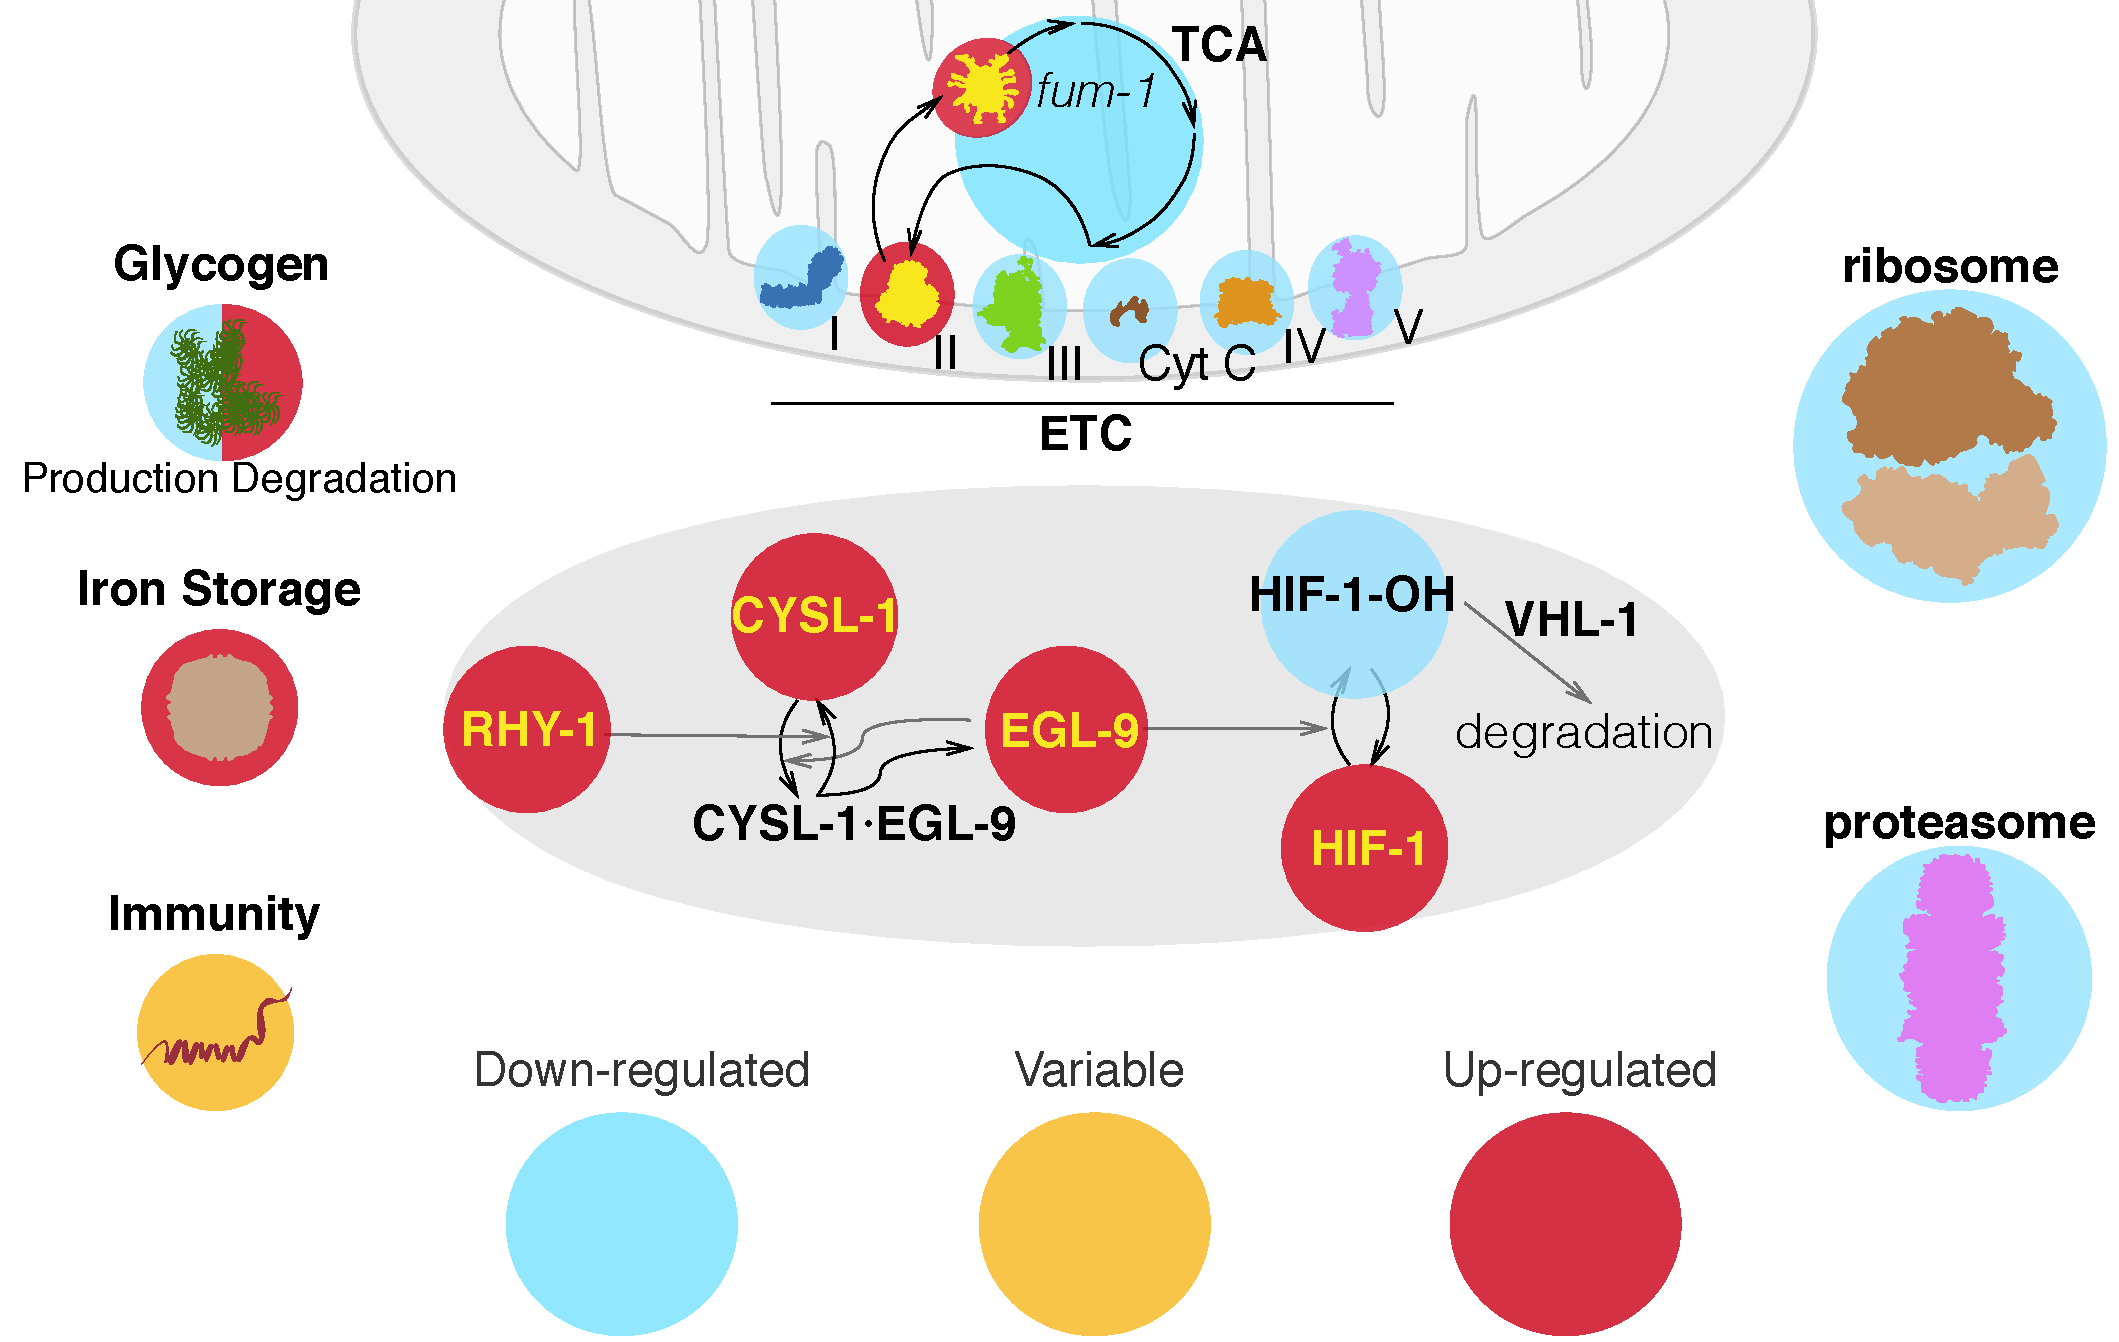
\includegraphics[width=.7\linewidth]{hypims/hif1genomewide.pdf}
\caption{
A graphic summary of the genome-wide effects of \hifp{} from our RNA-seq data.
}
\label{fig:genomewide}
\end{figure}

\subsubsection*{Bioenergetic pathways}
Our data shows that most of the enzymes involved in the TCA cycle and in the ETC
are down-regulated when \hifp{} is induced in agreement with the previous
literature~\citep{Semenza2012}.
However, the fumarase gene \gene{fum-1} and the mitochondrial complex II stood out
as notable exceptions to the trend, as they were up-regulated in every single
genotype that causes deployment of the hypoxia response. FUM-1 catalyzes the
reaction of fumarate into malate, and complex II catalyzes the reaction of
succinate into fumarate. Complex II has been identified as a source of reserve
respiratory capacity in neonatal rat cardiomyocytes previously~\citep{Pfleger2015}.
We found two energy reserve genes that were down-regulated by \hifp{}.
\gene{aagr-1} and \gene{aagr-2}, which are predicted to function in glycogen
catabolism~\citep{Sikora2010}.
Three distinct genes involved in energy reserve were up-regulated. These genes were
\gene{ogt-1}, which encodes O-linked GlcNac Transferase gene; \gene{T04A8.7},
encoding an ortholog of human glucosidase, acid beta (GBA); and \gene{T22F3.3},
encoding ortholog of human glycogen phosphorylase isozyme in the muscle (PYGM).

\subsubsection*{Protein synthesis and degradation}
\hif{} is also known to inhibit protein synthesis and translation in varied
ways.~\citep{Brugarolas2004}. Most reported effects of
\hifp{} on the translation machinery are posttranslational, and no reports to date
show transcriptional control of the ribosomal machinery in \cel{} by \hifp{}. We
used the WormBase Enrichment Suite Gene Ontology
dictionary~\citep{Angeles-Albores2016b} to extract 143 protein-coding genes
annotated as `structural constituents of the ribosome' and we queried whether
they were differentially expressed in our mutants. \egl{}, \vhl{}, \rhy{} and
\egl{};\vhl{} showed differential expression of 91 distinct ribosomal constituents
(not all constituents were detected in all genotypes). For every one of these
genotypes, these genes were always down-regulated. In contrast, \hif{} showed
up-regulation of a single ribosomal constituent.

Next, we asked whether \hifp{} has any transcriptional effects on the
proteasomal constituents; no such effects of \hifp{} on the proteasome
have been reported in \cel{}. Out of 40 WormBase-annotated proteasomal constituents,
we found 31 constituents that were differentially expressed in at least one of the
four genotypes that induce a hypoxic response. Every gene we found was down-regulated
in at least two out of the four genotypes we studied.

\section*{Discussion}
\subsection*{The \cel{} hypoxia pathway can be reconstructed entirely from
             RNA-seq data}
In this paper, we have shown that whole-organism transcriptomic phenotypes
can be used to reconstruct genetic pathways and to discern previously overlooked
or uncharacterized genetic interactions. We successfully reconstructed the hypoxia
pathway, and inferred order of action (\gene{rhy-1} activates \gene{egl-9},
\gene{egl-9} and \gene{vhl-1} inhibit \gene{hif-1}), and we were able to infer
from transcriptome-wide epistasis measurements that \gene{egl-9} exerts
\gene{vhl-1}-dependent and independent inhibition on \gene{hif-1}.

\subsection*{\hifp{} and the cellular environment}

In addition to reconstructing the pathway, our dataset allowed us
to observe a wide variety of physiologic changes that occur as a result of the
\hifp{}-dependent hypoxia response. In particular, we observed down-regulation of most
components of the TCA cycle and the mitochondrial electron transport chain with
the exceptions of \gene{fum-1} and the mitochondrial complex II.\@ The mitochondrial
complex II catalyzes the reaction of succinate into fumarate.
In mouse embryonic fibroblasts, fumarate has been
shown to antagonize \hifp{} prolyl hydroxylase domain (PHD) enzymes, which are
orthologs of \eglp{}~\citep{Sudarshan2009}.
If the inhibitory role of fumarate on PHD enzymes is conserved in \cel{},
upregulation of complex II by \hifp{} during hypoxia may increase
intracellular levels of fumarate, which in turn could lead to artificially high
levels of \hifp{}
even after normoxia resumes. The increase in fumarate produced by the complex
could be compensated by increasing expression of \gene{fum-1}. Increased fumarate
degradation allows \cel{} to maintain plasticity in the hypoxia pathway, keeping
the pathway sensitive to oxygen levels.

\subsection*{Interpretation of the non-classical epistasis in the hypoxia pathway}
The observation of almost 30 genes that exhibit a specific pattern of non-classical
epistasis suggests the existence of previously undescribed aspects of the hypoxia
pathway. Some of these non-classical epistases had been observed
previously~\citep{Ackerman2012,Romney2011,Luhachack2012}, but
no satisfactory mechanism has been proposed to explain this biology.
\citet{Romney2011} and \citet{Ackerman2012}
suggest that \hifp{} integrates information on iron concentration in the
cell to bind to the \ftna{} promoter, but could not definitively establish
a mechanism.
It is unclear why deletion of \gene{hif-1} induces \ftna{}
expression, deletion of \gene{egl-9} also causes induction of \ftna{} expression,
but deletion of \gene{vhl-1} removes this inhibition. Moreover, \citet{Luhachack2012}
have previously reported that certain genes important for the \cel{} immune response
against pathogens reflect similar expression patterns. Their interpretation
was that \gene{swan-1}, which encodes a binding partner to \eglp{}~\citep{Shao2010},
is important for modulating \hifp{} activity in some manner. The lack of a
conclusive double mutant analysis in this work means the role of SWAN-1 in
modulation of \hifp{} activity remains to be demonstrated. Nevertheless, mechanisms
that call for additional transcriptional modulators become less likely given the
number of genes with different biological functions that exhibit the same pattern.

\begin{figure}[tbhp]
\centering
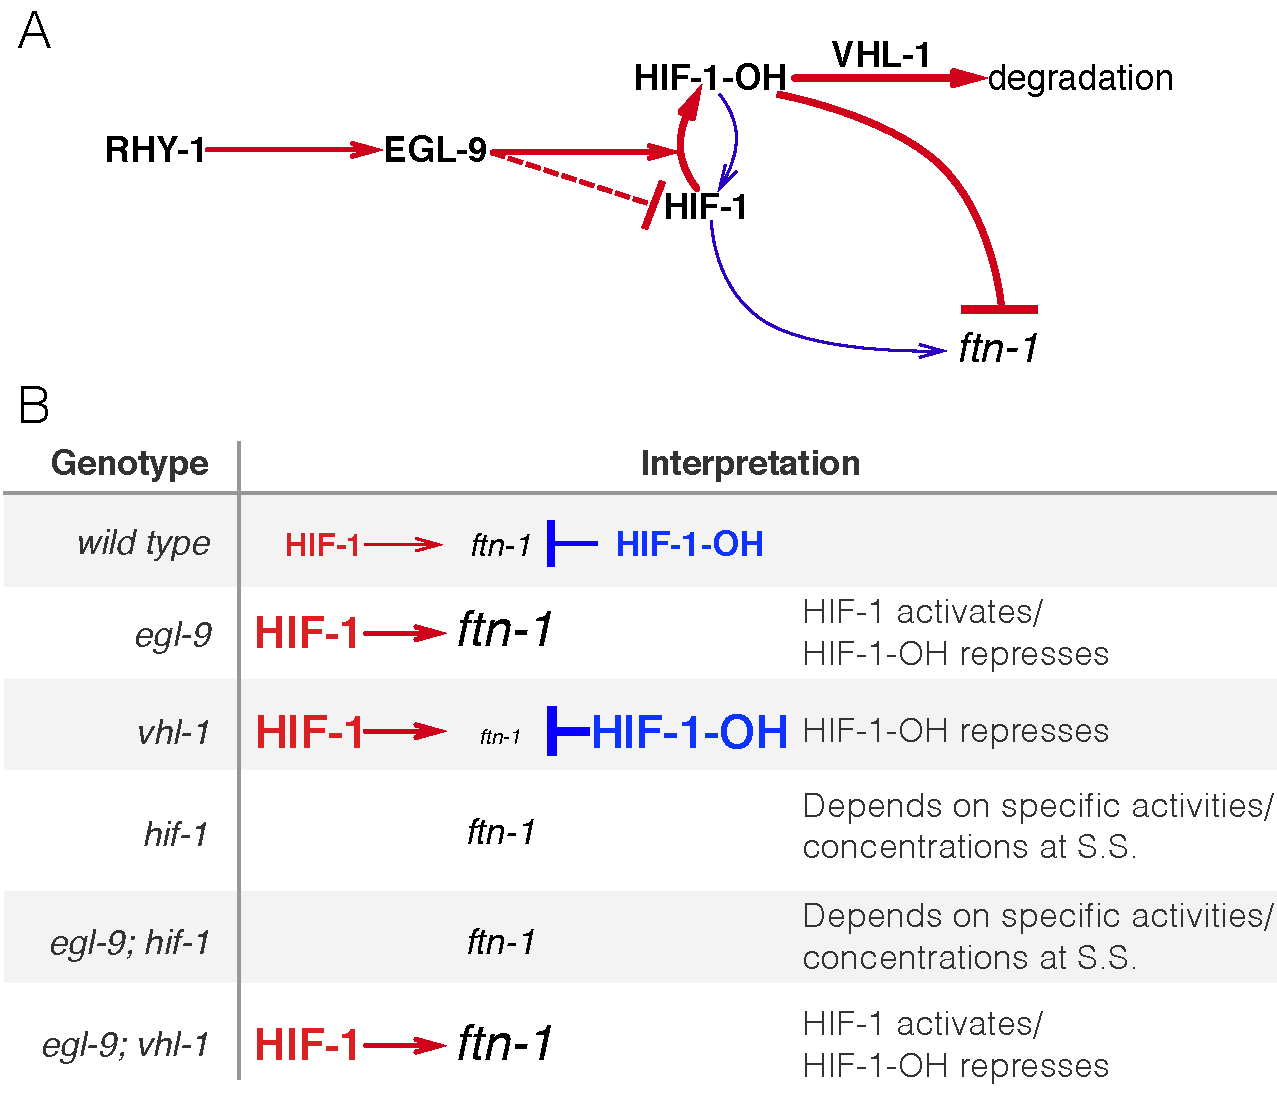
\includegraphics[width=.5\linewidth]{hypims/hif1oh_model.pdf}
\caption{
A hypothetical model showing a mechanism where \hifp{}-hydroxyl antagonises
\hifp{}.
\textbf{A}. Diagram showing that RHY-1 activates EGL-9.
EGL-9 hydroxylates HIF-1 in an oxygen dependent fashion. Under normoxia, HIF-1
is rapidly hydroxylated and only slowly does hydroxylated HIF-1 return to its
original state. EGL-9 can also inhibit HIF-1 in an oxygen-independent fashion.
HIF-1 hydroxyl is rapidly degraded in a VHL-1 dependent fashion. In our model,
HIF-1 and HIF-1 hydroxyl have opposing effects on transcription. The width of the
arrows represents the rates under normoxic conditions.
\textbf{B}. Table showing the effects of loss-of-function mutations on HIF-1 and
HIF-1 hydroxyl activity, showing how this can potentially explain the behavior
of \gene{ftn-1} in each case.  S.S = Steady-state.
}
\label{fig:hif1oh_table}
\end{figure}

One way to resolve this problem without invoking additional genes is to
consider \hifp{} as a protein with both activating and inhibiting states. In fact,
\hifp{} already exists in two states in \cel{}: unmodified \hifp{} and
\hifp{}-hydroxyl (\hifp{}-OH). Under this model, \hifp{}-hydroxyl antagonizes
the effects of \hifp{} for certain genes like \ftna{} or \nlp{}. Loss of
\gene{vhl-1} stabilizes \hifp{}-hydroxyl.
A subset of genes that are sensitive to \hifp{}-hydroxyl will be inhibited as a
result of the increase in the amount of this species, in spite of loss of
\gene{vhl-1} function also increasing the level of non-hydroxylated \hifp{}.
On the other hand, \egl{} selectively removes all \hifp{}-hydroxyl, stimulating
accumulation of \hifp{} and promoting gene activity. Whether deletion of \hif{}
is overall activating or inhibiting will depend on the relative activity of each
protein state under normoxia (see Fig.~\ref{fig:hif1oh_table}).

Multiple lines of circumstantial evidence that \hifp{}-hydroxyl plays a role
in the functionality of the hypoxia pathway. First, \hifp{}-hydroxyl is
challenging to study genetically because no mimetic mutations are available with
which to study the pure hydroxylated \hifp{} species. Second, although mutations in
the Von-Hippel Landau gene stabilize the hydroxyl species, they also increase the
quantity of non-hydroxylated \hifp{} by mass action.
Finally, since \hifp{} is detected low levels
in cells under normoxic conditions~\citep{Wang1993}, total \hifp{} protein
(unmodified \hifp{} plus \hifp{}-hydroxyl) is often tacitly assumed to be
vanishingly rare and therefore biologically inactive.

Our data show hundreds of genes that change expression in response
to loss of \gene{hif-1} under normoxic conditions. This establishes that there is
sufficient total \hifp{} protein to be biologically active.
Our analyses also revealed that \hif{} shares
positive correlations with \egl{}, \rhy{} and \vhl{}, and that each of these genotypes
also shows a secondary negative rank-ordered expression correlation with each other.
These cross-patterns between all loss of function of inhibitors of \hifp{} and
\hif{} can be most easily explained if \hifp{}-hydroxyl is biologically active.

A homeostatic argument can be made in favor of the activity of \hifp{}-hydroxyl.
At any point in time, the cell must measure the levels of
multiple metabolites at once. The \gene{hif-1}-dependent hypoxia
response integrates information from O$_2$, $\alpha$-ketoglutarate
(2-oxoglutarate) and iron concentrations in the cell. One way to
integrate this information is by encoding it only in the effective hydroxylation
rate of \hifp{} by \eglp{}. Then the dynamics in this system will evolve
exclusively as a result of the total amount of \hifp{} in the cell. Such a system
can be sensitive to fluctuations in the absolute concentration of
\hifp{}~\citep{Goentoro2009a}. Since the absolute levels of \hifp{} are low in
normoxic conditions, small fluctuations in protein copy-number represent can
represent a large fold-change in \hifp{} levels. These fluctuations would
not be problematic for genes that must be turned on only under conditions of severe
hypoxia---presumably, these genes would be associated with low affinity
sites for \hifp{}, so that they are only activated when \hifp{} levels are far
above random fluctuations.

For yet other sets of genes that must change expression in response to the hypoxia
pathway, it may not make as much sense to integrate metabolite information
exclusively via \eglp{}-dependent hydroxylation of \hifp{}. In particular, genes
that may function to increase survival in mild hypoxia may benefit from regulatory
mechanisms that can sense minor changes in environmental conditions and which
therefore benefit from robustness to transient changes in protein copy number.
Likewise, genes that are involved in iron or $\alpha$-ketoglutarate metabolism
(such as \ftna{}) may benefit from being able to sense, accurately, small and
consistent deviations from basal concentrations of these metabolites. For these
genes, the information may be better encoded by using \hifp{} and
\hifp{}-hydroxyl as an activator/repressor pair. Such circuits are
known to possess distinct advantages for controlling output in a manner that
is robust to transient fluctuations in the levels of their
components~\citep{Hart2012,Hart2013}.

Our RNA-seq data suggests that one of these atypical targets of \hifp{}
may be \rhyp{}. Although \gene{rhy-1} does not exhibit non-classical
epistasis, \hif{} and \eglhif{} both had increased expression levels of \gene{rhy-1}.
We speculate that if \gene{rhy-1} is controlled by both \hifp{} and \hifp{}-hydroxyl,
then this might imply that \hifp{} regulates the expression of its pathway (and
therefore itself) in a manner that is robust to total \hifp{} levels.

\subsection*{Insights into genetic interactions from vectorial phenotypes}

Here, we have described a set of straightforward methods that can be in theory
applied to any vectorial phenotype. Genome-wide methods afford a lot of information,
but genome-wide interpretation of the results is often extremely challenging.
Each method has its own advantages and disadvantages. We briefly discuss these
methods, their uses and their drawbacks.

Principal component analysis
is computationally tractable and clusters can often be visually detected with
ease. However, PCA can be misleading, especially when the dimensions represented
do not explain a very large fraction of the variance present in the data. In addition,
principal dimensions are the product of a linear combination of vectors, and therefore
must be interpreted with extreme care. In this case, the first principal dimension
separated genotypes that increase \hifp{} protein levels from those that decrease
it, but this dimension is a mix of vectors of change in gene expression. Although
PCA showed that there is information hidden in these genotypes, it was not enough
by itself to provide biological insight.

Whereas PCA operates on all genotypes simultaneously, correlation analysis is a
pairwise procedure that measures how predictable the gene
expression changes are in a mutant given the vector of expression changes in
another. Like PCA, correlation analysis is easy and fast to perform. Unlike PCA,
the product of a correlation analysis is a single number with a straightforward
interpretation. However, correlation analysis is particularly sensitive to outliers.
Although a common strategy is to rank-transform expression data to mitigate
outliers, rank-transformations do not remove the cross-patterns that appear when
feedback loops or other complex interactions are present between two genes.
Such cross-patterns can still lead to vanishing correlations if both patterns are
equally strong. Therefore, correlation analyses must take into account the possible
existence of systematic outliers. Moreover, correlation values must be measured
for both interactions in cross-patterned rank plots. Weighted correlations could
be informative for ordering genes along pathways.
A drawback of correlation
analysis is that the number of pairwise comparisons that must be made increases
combinatorially, though strategies could be used to decrease the total number of
effective comparisons.

Epistasis plots are a novel way to visualize epistasis in vectorial phenotypes.
Here, we have shown how an epistasis plot can be used to identify interactions
between two single mutants and a double mutant. In reality, epistasis plots
can be generated for any set of measurements involving a set of $N$ mutants and
an $N$-mutant genotype. Epistasis plots can accumulate an arbitrary number of
points within them, possess a rich structure that can be visualized and have
straightforward interpretations for special slope values.

Another way to analyze epistasis is via general linear models (GLMs) that include
interaction terms between two or more genes. In this way, GLMs can quantify
the epistatic effect of an interaction on single genes. We and
others~\citep{Dixit2016,Angeles-Albores2016a} have previously used GLMs to identify
gene sets that are epistatically regulated by two or more inputs. While powerful,
GLMs suffer from the multiple comparison problem. Correcting for false positives
using well-known multiple comparison corrections such as FDR~\citep{Storey2003}
tends to increase false negative rates.  Moreover, since GLMs attempt to estimate
effect magnitudes for individual gene or isoform expression levels, they
effectively treat each gene as an independent quantity, which prevents better
estimation of the magnitude and direction of the epistasis between two genes.

Epistasis plots do not suffer from the multiple comparison problem because the
number of tests performed is orders of magnitudes smaller than the number
of tests performed by GLMs. Ideally, in an epistasis plot we need only perform
3 tests---rejection of additive, unbranched and suppressive null models---compared
with the tens of thousands of tests that are performed in GLMs. Moreover, the
magnitude of epistasis between two genes can be estimated using hundreds of genes,
which greatly improves the statistical resolution of the epistatic coefficient.
This increased resolution is important because the size and magnitude of the
epistasis has specific consequences for the type of pathway that is expected.

Any quantitative use of genome-wide datasets requires a good experimental setup.
Here, we have demonstrated that whole-organism RNA-seq can be used to dissect
molecular pathways in exquisite detail when paired with experimental designs that
are motivated by classical genetics. Much more research will be necessary
to understand whether epistasis has different consequences in the microscopic
realm of transcriptional phenotypes than in the macroscopic world that geneticists
have explored previously. Our hope is that these tools, coupled with the classic
genetics experimental  designs, will reveal hitherto unknown aspects of genetics
theory.

\section*{Methods}
\label{sec:methods}
\subsection*{Nematode strains and culture}
Strains used were N2 wild-type Bristol,
CB5602 \gene{vhl-1}(\emph{ok161}),
CB6088 \gene{egl-9}(\emph{sa307})~\gene{hif-1}(\emph{ia4}),
CB6116 \gene{egl-9}(\emph{sa307});\gene{vhl-1}(\emph{ok161}),
JT307 \gene{egl-9}(\emph{sa307}),
ZG31 \gene{hif-1}(\emph{ia4}),
RB1297 \gene{rhy-1}(\emph{ok1402}).
All lines were grown on standard
nematode growth media (NGM) plates seeded with OP50 \ecol{} at 20\degree{}C
(Brenner 1974).

\subsection*{RNA Isolation}
Unsynchronized lines were grown on NGM plates at 20C and eggs harvested by
sodium hypochlorite treatment. Eggs were plated on 6 to 9 6cm NGM plates
with ample OP50 \ecol{} to avoid starvation and grown at
20\degree{}C.  Worms were staged and harvested based on the time after plating,
vulva morphology and the absence of eggs.  Approximately 30--50 non-gravid young
adults were picked and placed in 100$\mu$L of TE pH 8.0 at 4\degree{}C in
$0.2$mL PCR tubes.   After settling and a brief spin in microcentrifuge
approximately $80\mu$L of TE (Ambion AM 9849) was removed from the top of the
sample and individual replicates
were snap frozen in liquid N2. These replicate samples were then digested with
Proteinase K (Roche Lot No. 03115 838001 Recombinant Proteinase K PCR Grade) for
15min at 60\degree{} in the presence of 1\% SDS and 1.25$\mu$L
RNA Secure (Ambion AM 7005). RNA samples were then taken up in 5 Volumes of
Trizol (Tri Reagent Zymo Research) and processed and treated with DNase I using
Zymo MicroPrep RNA Kit (Zymo Research Quick-RNA MicroPrep R1050).
RNA was eluted in RNase-free water and divided into aliquots and stored at
-80\degree{}C. One aliquot of each replicate was analyzed using a NanoDrop (Thermo
Fisher) for impurities, Qubit for concentration and then analyzed on an Agilent
2100 BioAnalyzer (Agilent Technologies).
Replicates were selected that had RNA integrity numbers (RIN) equal or greater
than 9.0 and showed no evidence of bacterial ribosomal bands, except for the
ZG31 mutant where one of three replicates had a RIN of 8.3.

\subsection*{Library Preparation and Sequencing}
10ng of quality checked total RNA from each sample was
reverse-transcribed into cDNA using the Clontech SMARTer Ultra Low Input RNA for
Sequencing v3 kit (catalog \#634848) in the SMARTSeq2 protocol
~\citep{Picelli2014}.  RNA was denatured at 70$\degree{}$C for 3 minutes
in the presence of dNTPs, oligo dT primer and spiked-in quantitation standards
(NIST/ERCC from Ambion, catalog \#4456740).  After chilling to 4$\degree{}$C, the
first-strand reaction was assembled using the LNA TSO primer described in
\citet{Picelli2014}, and run at 42$\degree{}$C for 90 minutes, followed by
denaturation at 70$\degree{}$C for 10 minutes.  The entire first strand reaction
was then used as template for 13 cycles of PCR using the Clontech v3 kit.
Reactions were cleaned up with 1.8X volume of Ampure XP SPRI beads (catalog
\#A63880) according to the manufacturer’s protocol.  After quantification using
the Qubit High Sensitivity DNA assay, a 3ng aliquot of the amplified cDNA was
run on the Agilent HS DNA chip to confirm the length distribution of the
amplified fragments.  The median value for the average cDNA lengths from all
length distributions was 1076bp.  Tagmentation of the full length cDNA for
sequencing was performed using the Illumina/Nextera DNA library prep kit (catalog
\#FC-121--1030).  Following Qubit quantitation and Agilent BioAnalyzer profiling,
the tagmented libraries were sequenced. Libraries were sequenced on Illumina
HiSeq2500 in single read mode with the read length of 50nt to an average depth
of 15 million reads per sample following manufacturer's instructions. Base calls
were performed with RTA 1.13.48.0 followed by conversion to FASTQ with bcl2fastq
1.8.4. Spearman correlation of the transcripts per million (TPM) for each
genotype showed that every pairwise correlation within genotype was $>0.9$.

\subsection*{Read Alignment and Differential Expression Analysis}
We used Kallisto to perform read pseudo-alignment and performed differential
analysis using Sleuth. We fit a general linear model for a transcript $t$ in
sample $i$:

\begin{equation}
  y_{t,i} = \beta_{t, 0} + \beta_{t, genotype}\cdot{}X_{t, i} +
  \beta_{t, batch}\cdot{}Y_{t, i} + \epsilon_{t, i}
\end{equation}

where $y_{t, i}$ are the logarithm transformed counts; $\beta_{t, genotype}$ and
$\beta_{t, batch}$ are parameters of the model, and which can be interpreted as
biased estimators of the log-fold change; $X_{t, i}, Y_{t, i}$ are indicator
variables describing the conditions of the sample; and $\epsilon_{t, i}$ is the
noise associated with a particular measurement.

\subsection*{Genetic Analysis, Overview}
Genetic analysis of the processed data was performed in Python 3.5. Our scripts
made extensive use of the Pandas, Matplotlib, Scipy, Seaborn, Sklearn, Networkx,
Bokeh, PyMC3, and TEA libraries~\citep{Team2014,McKinney2011,Oliphant2007,
Pedregosa2012,Salvatier2015,VanDerWalt2011,Hunter2007,Angeles-Albores2016,Waskom}.
Our analysis is available in a Jupyter Notebook~\citep{Perez2007}. All code and
required data (except the raw reads) are available at
\url{https://github.com/WormLabCaltech/mprsq} along with version-control
information. Our Jupyter Notebook and interactive graphs for this project can be
found at \url{https://wormlabcaltech.github.io/mprsq/}. Raw reads were deposited
in the Short Read Archive under the study accession number SRP100886.


\subsection*{Weighted Correlations}
Pairwise correlations between transcriptomes where calculated by first identifying
the set of differentially expressed genes (DEGs) common to both transcriptomes under
analysis. DEGs were then rank-ordered according to their regression coefficient,
$\beta$.\ Bayesian robust regressions were performed using a Student-T distribution.
Bayesian analysis was performed using the PyMC3 library~\citep{Salvatier2015}
(\texttt{pm.glm.families.StudenT} in Python). If the correlation has an average
value $>1$, the correlation coefficient was set to 1.

Weights were calculated as the proportion of genes that were $<1.5$ standard
deviations away from the primary regression out of the entire set of shared DEGs
for each transcriptome.

\subsection*{Epistasis Analysis}
For a double mutant $X^-Y^-$, we used the single mutants $X^-$ and $Y^-$ to
find expected value of the coefficient for a double mutant under an additive model
for each isoform $i$.
Specifically,
\begin{equation}
  \beta_{\mathrm{Add},i} = \beta_{X,i} + \beta_{Y,i}.
\end{equation}

Next, we find the difference, $\Delta_i$, between the observed double mutant
expression coefficient, $\beta_{XY, \mathrm{Obs},i}$, and the predicted
expression coefficient under an additive model for each isoform $i$.

To calculate the transcriptome-wide epistasis coefficient, we plotted
($\beta_{\mathrm{Add},i}, \Delta_i$) and found the line of best fit using
orthogonal distance regression using the \texttt{scipy.odr} package in Python.
We performed
non-parametric bootstrap sampling of the ordered tuples with replacement using
5,000 iterations to generate a probability distribution of slopes of best fit.

There are as many models as epistatic relationships. For quantitative phenotypes,
epistatic relationships (except synthetic interactions) can be generally
expressed as:

\begin{equation}
  \beta_{XY} = \sum_{g\in G} \lambda_g \beta_g,
  \label{eq:epi}
\end{equation}

where $P_i$ is the quantitative phenotype belonging to the genotype $i$; $G$ is
the set of single mutants $\{X, Y\}$ that make up the double mutant, $XY$; and
$\lambda_g$ is the contribution of the phenotype $P_g$ to $P_{XY}$.
Additive interactions between genes are the result of setting $\lambda_g=1$. All
other relationships correspond to setting  $\lambda_X=0,~\lambda_Y=1$ or
$\lambda_X=1,~\lambda_Y=0$.

A given epistatic interaction can be simulated by predicting the double mutant
phenotype under that interaction and re-calculating the y-coordinates. The
recalculated y-coordinates can then be used to predict the possible epistasis
coefficients for the cases where $X$ is epistatic over $Y$, and $Y$ is epistatic
over $X$.

To select between theoretical models, we implemented an approximate Bayesian
Odds Ratio. We defined a free-fit model, $M_1$, that found the line of best fit
for the data:

\begin{equation}
  P(\alpha~|M_1, D) \propto \prod_{(x_i, y_i, \sigma_i)\in D}
  \exp{\frac{
            (y_i - \alpha\cdot x_i)^2
            } % numerator
            {
            2\sigma_i
            } % denominator
            } \cdot (1+\alpha^2)^{-3/2},
  \label{eq:free_model}
\end{equation}

where $\alpha$ is the slope of the model to be determined, $x_i, y_i$ were the
x- and y-coordinates of each point respectively, and $\sigma_i$ was the standard
error associated with the y-value. We minimized the
negative logarithm of equation~\ref{eq:free_model} to obtain the most likely
slope given the data, $D$ (\texttt{scipy.optimize.minimize} in Python). Finally,
we approximated the odds ratio as:

\begin{equation}
  OR = \frac{
  P(D~|\alpha^*, M_1)\cdot (2\pi)^{1/2}\sigma_{\alpha^*} % numerator
  }{P(D~| M_i)}, % denominator
\end{equation}

where $\alpha^*$ is the slope found after minimization, $\sigma_\alpha^*$ is the
standard deviation of the parameter at the point $\alpha^*$ and $P(D~|M_i)$ is the
probability of the data given the parameter-free model, $M_i$.

\subsection*{Enrichment Analysis}
Tissue, Phenotype and Gene Ontology Enrichment Analysis were carried out using
the WormBase Enrichment Suite for Python~\citep{Angeles-Albores2016b,
Angeles-Albores2016}.



\subsubsection*{Author Contributions:}
This work was supported by HHMI with whom PWS is an investigator
and by the Millard and Muriel Jacobs Genetics and Genomics Laboratory at
California Institute of Technology.
All strains were provided by the CGC, which is funded by NIH Office of Research
Infrastructure Programs (P40 OD010440).
This article was written with support of the Howard Hughes Medical Institute.
This article wouldn't be possible without help from Dr.\_ Igor Antoshechkin who
performed all sequencing.
We thank Hillel Schwartz for all of his careful advice.
We would like to thank Jonathan Liu, Han Wang, and Porfirio Quintero for helpful
discussion.

  % \printbibliography[heading=subbibliography]
\end{refsection}

\chapter{Qualitative or quantitative allelic series}
\begin{refsection}
  % \newcommand{\dicty}{\emph{D.~discoideum}}

% gene names
\newcommand{\nlp}{\emph{\mbox{nlp-31}}}
\newcommand{\ftna}{\emph{\mbox{ftn-1}}}
\newcommand{\ftnb}{\emph{\mbox{ftn-2}}}
\newcommand{\cysl}{\emph{\mbox{cysl-1}}}
\newcommand{\nog}{\emph{\mbox{nog-1}}}
\newcommand{\nhr}{\emph{\mbox{nhr-57}}}
\newcommand{\lam}{\emph{\mbox{lam-3}}}

\newcommand{\fog}{\emph{\mbox{fog-2(lf)}}}
\newcommand{\egl}{\emph{\mbox{egl-9}(lf)}}
\newcommand{\rhy}{\emph{\mbox{rhy-1}(lf)}}
\newcommand{\vhl}{\emph{\mbox{vhl-1}(lf)}}
\newcommand{\eglvhl}{\emph{\mbox{egl-9(lf);vhl-1(lf)}}}
\newcommand{\eglhif}{\emph{\mbox{egl-9(lf)}~\mbox{hif-1(lf)}}}
\newcommand{\hif}{\emph{\mbox{hif-1(lf)}}}

% protein names
\newcommand{\eglp}{EGL-9}
\newcommand{\rhyp}{RHY-1}
\newcommand{\nogp}{NOG-1}
\newcommand{\vhlp}{VHL-1}
\newcommand{\hifp}{HIF-1}
\newcommand{\fogp}{FOG-2}
\newcommand{\nhrp}{NHR-57}
\newcommand{\lamp}{LAM-3}
\newcommand{\cyslp}{CYSL-1}

% DE genes numbers:
\newcommand{\egln}{1,806}
\newcommand{\rhyn}{2,103}
\newcommand{\vhln}{689}
\newcommand{\eglvhln}{2,376}
\newcommand{\hifn}{546}
\newcommand{\eglhifn}{404}
\newcommand{\fogn}{2090}
\newcommand{\total}{5,671} % isoforms!!!!
% \newcommand{\inall}{53}
% \newcommand{\allup}{10}
% \newcommand{\alldown}{13}

% downstream targets
\newcommand{\egltargets}{126}
\newcommand{\rhytargets}{0}
\newcommand{\vhltargets}{45} % 44 genes, minus vhl-1 (IDed due to deletion)
\newcommand{\hiftargets}{195}
\newcommand{\hifohtargets}{31}


% website commands
\newcommand{\website}{
            \url{https://wormlabcaltech.github.io/Angeles_Leighton_2016/}
            }
\newcommand{\webref}{
\href{https://wormlabcaltech.github.io/Angeles_Leighton_2016/}{website}}

% more space between rows
\newcommand{\ra}[1]{\renewcommand{\arraystretch}{#1}}

\section*{Abstract}
\textbf{
RNA-seq is commonly used to identify genetic modules that respond to perturbations.
In single cells, transcriptomes have been used as phenotypes, but this concept
has not been applied to whole-organism RNA-seq. Linear models can quantify
expression effects of individual mutants and identify epistatic effects in double
mutants. However, interpreting these high-dimensional measurements is unintuitive.
We developed a single coefficient to quantify transcriptome-wide epistasis which
accurately reflects the underlying interactions. To demonstrate the power of our
approach, we sequenced four single and two double C. elegans mutants. From these
mutants, we successfully reconstructed the known hypoxia pathway. Using this
approach, we uncovered a class of 31 genes that have opposing changes in expression
in \egl{} and \vhl{} but the \eglvhl{} mutant phenocopies \egl{}.
These changes violate the classical model of HIF-1 regulation, but can be explained
by postulating a role of hydroxylated HIF-1 in transcriptional control.
}
\vspace{10mm}


\section*{Introduction}
\label{sec:introduction}
Genetic analysis of molecular pathways has traditionally been performed
through epistatis analysis. Generalized epistasis indicates that two genes interact
functionally; such interaction can involve the direct interaction of their
products or the interaction of any consequence of their function (small molecules,
physiological or behavioral effects)~\citep{Huang2006}. If two
genes interact, and the mutants of these genes have a quantifiable phenotype,
the double mutant of interacting genes will have a phenotype that is not the sum
of the phenotypes of the single mutants that make up its genotype. Epistasis
analysis remains a cornerstone of genetics today~\citep{Phillips2008}.


Recently, biological studies have shifted in focus from studying single
genes to studying all genes in parallel. In particular,
RNA-seq~\citep{Mortazavi2008} enables biologists to
identify genes that change expression in response to a perturbation. Gene expression
profiling using RNA-seq has become much more sensitive thanks to deeper and more
frequent sequencing due to lower sequencing costs~\citep{Metzker2010},
better and faster abundance quantification~\citep{Patro2014,Bray2016,Patro2015},
and improved differential expression analysis
methods~\citep{Pimentel2016,Trapnell2013}. RNA-seq has been
successfully used to identify genetic modules involved in a variety of processes,
including T-cell regulation~\citep{Singer2016,Shalek2013}, the
\emph{Caenorhabditis~elegans} (\cel{}) linker
cell migration~\citep{Schwarz2012}, and planarian stem cell
maintenance~\citep{VanWolfswinkel2014,Scimone2014}. For the most part, the role of
transcriptional profiling has been restricted to target gene identification.

Although transcriptional profiling has been primarily used for descriptive purposes,
transcriptomic phenotypes have previously been used to make genetic inferences.
Microarray analyses in \emph{S. cerevisiae} and \dicty{} were used to show
that transcriptomes can be interpreted to infer genetic relationships in simple
eukaryotes~\citep{Hughes2000, VanDriessche2005}.\@ eQTL studies in
many organisms, from yeast to humans, have established the usefulness of
transcriptomic phenotypes for population genetics studies~\citep{Brem2002,Schadt2003,
Li2006,King2014}. In cell culture, single-cell RNA-seq has seen significant
progress towards using transcriptomes as phenotypes with which to test genetic
interactions~\citep{Adamson2016,Dixit2016}.
More recently, we have identified a new developmental state
of \cel{} using whole-organism transcriptome profiling~\citep{Angeles-Albores2016a}.
To investigate the ability of whole-organism transcriptomes to serve as quantitative
phenotypes for epistasis analysis in metazoans, we sequenced the transcriptomes of
of four well-characterized loss of function mutants in the \cel{} hypoxia
pathway~\citep{Epstein2001,Shen2006,Shao2009,Jiang2001}.

% carmie:
Metazoans depend on the presence of oxygen in sufficient concentrations to
support aerobic metabolism. Genetic pathways evolved to rapidly respond to any
acute or chronic changes in oxygen levels at the cellular or organismal level.
Biochemical and genetic approaches identified the Hypoxia Inducible Factors
(HIFs) as an important group of oxygen-responsive genes that are involved in a
broad range of human pathologies~\citep{Semenza2012}.

Hypoxia Inducible Factors are highly conserved in metazoans~\citep{Loenarz2011}.
A common mechanism for hypoxia-response induction is heterodimerization between a
HIF$\alpha$ and a HIF$\beta$ subunit; the heterodimer then initiates
transcription of target genes~\citep{Jiang1996}. The number and complexity of
HIFs varies throughout metazoans, with humans having three HIF$\alpha$ subunits
and two HIF$\beta$ subunits, whereas in the roundworm \cel{} there is a single
HIF$\alpha$ gene, \gene{hif-1}~\citep{Jiang2001} and a single HIF$\beta$
gene, \gene{ahr-1}~\citep{Powell-Coffman1998}. HIF target genes have been implicated
in a wide variety of cellular and extracellular processes including glycolysis,
extracellular matrix modification, autophagy and immunity~\citep{Semenza1994,
Bishop2004,Shen2005,Bellier2009,Semenza2012}.

Levels of HIF$\alpha$ proteins tend to be tightly regulated. Under conditions of
normoxia, \hifp{}$\alpha$ exists in the cytoplasm and partakes in a futile cycle
of continuous protein production and rapid degradation~\citep{Huang1996}.
\hifp{}$\alpha$ is hydroxylated by three proline hydroxylases
in humans (PHD1, PHD2 and PHD3) but is only hydroxylated by one proline
hydroxylase (\eglp{}) in \cel{}~\citep{Kaelin2008}. \hifp{} hydroxylation
increases its binding affinity to Von Hippel Lindau Tumor Suppressor 1
(\vhlp{}), which allows ubiquitination of \hifp{} leading to its subsequent
degradation. In \cel{}, \eglp{} activity is inhibited by binding of \cyslp{},
and \cyslp{} activity is in turn inhibited at the protein level by \rhyp{},
possibly by post-translational modifications to \cyslp{}~\citep{Ma2012} (see
Fig.~\ref{fig:pathway}).

% heatmap
\begin{figure}[tbhp]
\centering
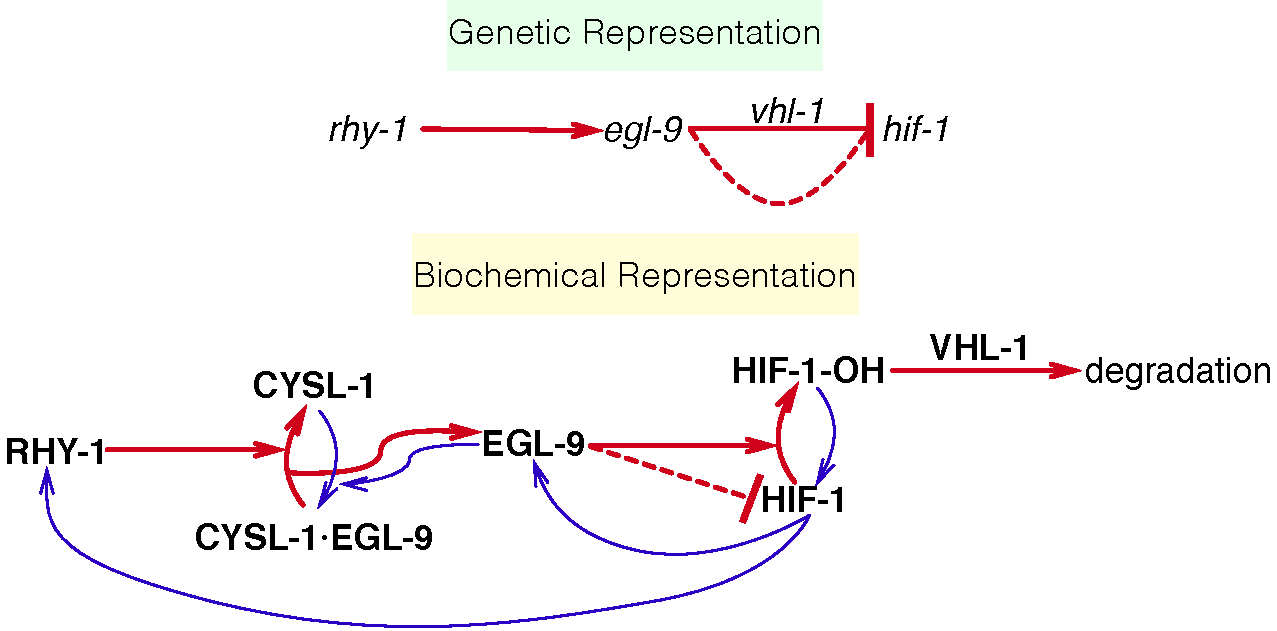
\includegraphics[width=.7\linewidth]{hypims/HIF1pathway.pdf}
\caption{
Genetic and biochemical representation of the hypoxia pathway in \cel{}.
Red arrows are arrows that lead to inhibition of \hifp{}, and blue arrows
are arrows that increase \hifp{} activity or are the result of \hifp{} activity.
\eglp{} is known to exert \gene{vhl-1}-dependent and independent repression
on \hifp{} as shown in the genetic diagram. The \gene{vhl-1}-independent
repression of \hifp{} by \eglp{} is denoted by a dashed line and is not dependent
on the hydroxylating activity of \eglp{}.
Technically, RHY-1 inhibits CYSL-1, which in turn inhibits EGL-9, but this
interaction was abbreviated in the genetic diagram for clarity.
}
\label{fig:pathway}
\end{figure}

Here, we show that transcriptomes contain robust signals that can be
used to infer relationships between genes in complex metazoans by reconstructing
the hypoxia pathway in \cel{} using RNA-seq.
Furthermore, we show that the phenomenon of phenotypic epistasis, a hallmark of
genetic interaction, holds at the molecular systems level.
We also demonstrate that transcriptomes contain sufficient information, under
certain circumstances, to order genes in a pathway using only single mutants.
Finally, we were able to identify genes that appear to be downstream of \gene{egl-9}
and \gene{vhl-1}, but do not appear to be targets of \gene{hif-1}.
Using a single set of genome-wide measurements, we were able to observe and
quantitatively assess  significant fraction of the known transcriptional
effects of \gene{hif-1} in \cel{}.
A complete version of the analysis, with ample documentation, is available at
\url{https://wormlabcaltech.github.io/mprsq}.

\section*{Results}
\subsection*{The hypoxia pathway controls thousands of genes in \cel{}}
\label{sub:summary}

We selected four single mutants within the hypoxia pathway for expression profiling:
\egl{} (\emph{sa307}), \rhy{} (\emph{ok1402}), \vhl{} (\emph{ok161}), \hif{} (\emph{ia4}).
We also sequenced the transcriptomes of two double mutants, \eglvhl{} (\emph{sa307},
\emph{ok161}) and \eglhif{} (\emph{sa307}, \emph{ia4}) as well as wild-type N2 as
a control sample. Each genotype  was sequenced in triplicate at a depth of 15
million reads. We performed whole-organism RNA-seq of these mutants at a moderate
sequencing depth ($\sim7$ million mapped reads for each individual replicate)
under normoxic conditions. For single samples, we identified around 22,000 different
isoforms per sample, which allowed us to measure differential expression of 18,344
isoforms across all replicates and genotypes (this constitutes  $\sim$70\% of
the protein coding isoforms in \cel{}).
We also included in our analysis a \fog{} (\emph{q71}) mutant which we have previously
studied~\citep{Angeles-Albores2016a}, because \gene{fog-2} is not reported to
interact with the hypoxia pathway.
We analyzed our data using a general linear model on
logarithm-transformed counts. Changes in gene expression are reflected in the
regression coefficient, $\beta$ which is specific to each isoform within a genotype.
Statistical significance is achieved when the q-values for each $\beta$ (p-values
adjusted for multiple testing) are less than 0.1. Genes that are significantly
altered between wild-type and a given mutant have $\beta$ values that are
statistically significantly different from 0.  These coefficients are not equal
to the average log-fold change per gene, although they are loosely related to
this quantity. Larger magnitudes of $\beta$ correspond to larger perturbations.
These coefficients can be used to study the RNA-seq data in question.

In spite of the moderate sequencing depth, transcriptome profiling of the hypoxia
pathway revealed that this pathway controls thousands of genes in \cel{}. The
\egl{} transcriptome showed differential expression of \egln{} genes. Similarly,
\rhyn{} genes were differentially expressed in \rhy{} mutants. The \vhl{}
transcriptome showed considerably fewer differentially expressed genes (\vhln{}),
possibly because it is a weaker controller of \hif{} than
\egl{}~\citep{Shao2009}. The \egl{};\vhl{} double mutant transcriptome showed
\eglvhln{} differentially expressed genes. The \hif{} mutant also showed a
transcriptomic phenotype involving \hifn{} genes. The \eglhif{} double mutant
showed a similar number of genes with altered expression (\eglhifn{} genes, see
Table~\ref{tab:genes}).

\begin{table}[tbhp]
  \centering
  \begin{tabular}{lr}
    \toprule{}
    Genotype & Differentially Expressed Genes \\
    \midrule{}
    \egl{} & \egln{}\\
    \rhy{} & \rhyn{}\\
    \vhl{} & \vhln{}\\
    \eglvhl{} & \eglvhln{}\\
    \eglhif{} & \eglhifn{}\\
    \fog{} & \fogn{}\\
    \bottomrule{}
  \end{tabular}
  \caption{Number of differentially expressed genes in each mutant.}
\label{tab:genes}
\end{table}

\subsection*{Principal Component Analysis visualizes epistatic relationships between genotypes}
\label{sub:Clustering}

Principal Component Analysis (PCA) is a well-known technique in bioinformatics that is
used to identify relationships between high dimensional data points~\citep{Yeung2001}
We performed PCA on our data to examine whether each genotype clustered in a biologically
relevant manner. PCA identifies the vector that can explain most of the variation
in the data;this is called the first PCA dimension. Using PCA, one can identify
the first $n$ dimensions that can explain more than 95\% of the variation in the
data. Sample clustering in these $n$ dimensions often indicates biological
relationships between the data, although interpreting PCA dimensions can be
difficult.

After applying PCA, we expected \hif{} to cluster near \eglhif{}, because
\hif{} exhibits no phenotypic defects under normoxic conditions, in contrast to
\egl{}, which exhibits an egg-laying (Egl) phenotype in the same environment.
In \eglhif{} mutants the Egl phenotype of \egl{} mutants is suppressed and instead
the grossly wild-type phenotype of \hif{} is observed. On the other hand, we
expected \egl{}, \rhy{}, \vhl{} and \eglvhl{} to form a separate cluster since
each of these genotypes is Egl and has a constitutive hypoxic response. Finally,
we included as a negative control a \fog{} mutant we have analyzed
previously~\citep{Angeles-Albores2016a}. This data was obtained at a different
time from the other genotypes, so we included a batch-normalization term in our
equations to account for this. Since \gene{fog-2} has not been described
to interact with the hypoxia pathway, we expected that it should appear far away
from either cluster.

The first dimension of the PCA analysis was able to discriminate between mutants
that have constitutive high levels of \hifp{} and mutants that have no \hifp{},
whereas the second dimension was able to discriminate between mutants within the
hypoxia pathway and outside the hypoxia pathway (see Fig.~\ref{fig:pca}).
Therefore expression profiling measures enough signal to cluster genes in a
meaningful manner in complex metazoans.

\begin{figure}[tbhp]
\centering
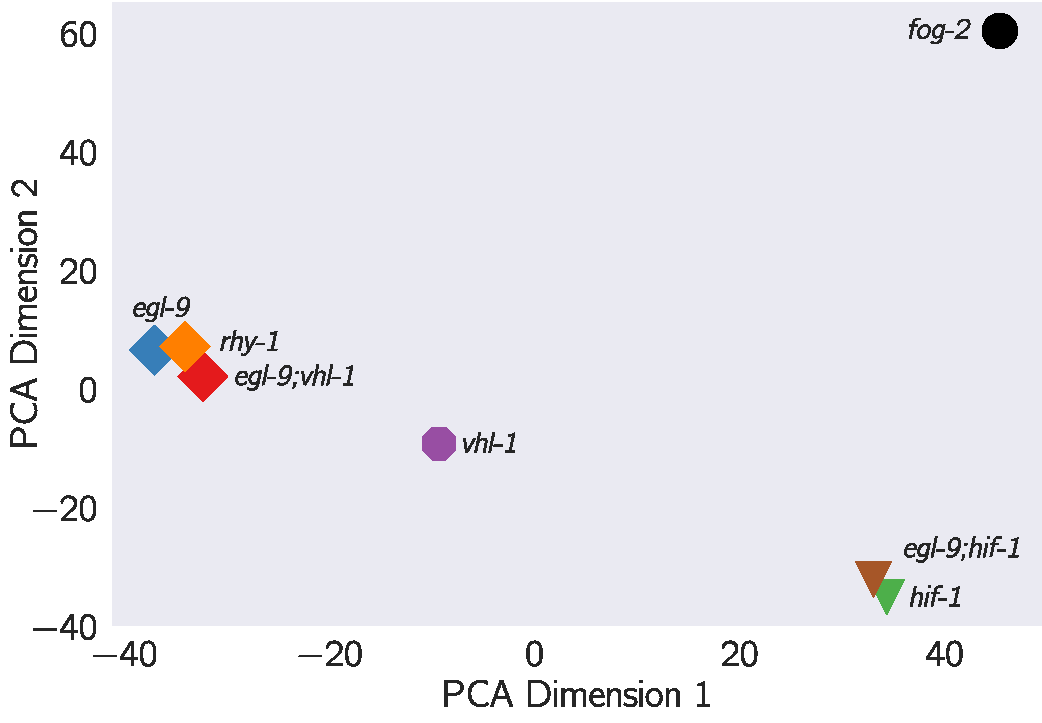
\includegraphics[width=0.5\linewidth]{hypims/pca.pdf}
\caption{
Principal component analysis of various \cel{} mutants. Genotypes that have an
activated hypoxia response (\emph{i.e}, \egl{}, \vhl{}, and \rhy{}) cluster far
from \hif{}. \hif{} clusters with the suppressed \eglhif{} double mutant.
The \fog{} transcriptome, used as an outgroup, is far away from either cluster.
}
\label{fig:pca}
\end{figure}

\subsection*{Reconstruction of the hypoxia pathway from first genetic principles}
\label{sec:reconstruct}
Having shown that the signal in the mutants we selected was sufficient to
cluster mutants using the values of the regression coefficients $\beta$, we set
out to reconstruct the hypoxia pathway from genetic first principles. In general,
to reconstruct a pathway, we must first assess whether two genes act on the same
phenotype. If they do not act on the same phenotype (the set of commonly differentially
regulated genes between two mutants is empty), these mutants are independent.
If they are not independent, then two mutants have a shared transcriptomic
phenotype (STP)---a set of genes or isoforms that are differentially expressed in
both mutants, without taking into account what direction they change in. In this
case, we must measure whether these genes act additively or epistatically on the
measured phenotype; if there is epistasis we must measure whether it is
positive or negative, in order to assess whether the epistatic relationship is a
genetic suppression or a synthetic interaction.

\subsubsection*{Genes in the hypoxia mutant act on the same transcriptional phenotype}
\label{sec:phenotypes}
We observed that all the hypoxia mutants had significant shared transcriptomic
phenotypes (fraction of the transcriptomes that was shared between mutants
ranged from a minimum of 6.8\% shared between \hif{} and \eglvhl{} to a maximum
of 31\% shared genes between \egl{} and \eglvhl{}). For comparison, we also
analyzed a previously published \fog{} transcriptome~\citep{Angeles-Albores2016a}.
The \gene{fog-2} gene is involved in masculinization of the \cel{} germline,
which enables sperm formation, and is not known to be involved in the hypoxia
pathway. The hypoxia pathway mutants and the \fog{} mutant also showed shared
transcriptomic phenotypes (3.6\%--12\% genes), but correlations between
expression level changes were considerably weaker (see below), suggesting that
there is minor cross-talk between these pathways.


% genetic correlations
\begin{figure}[tbhp]
\centering
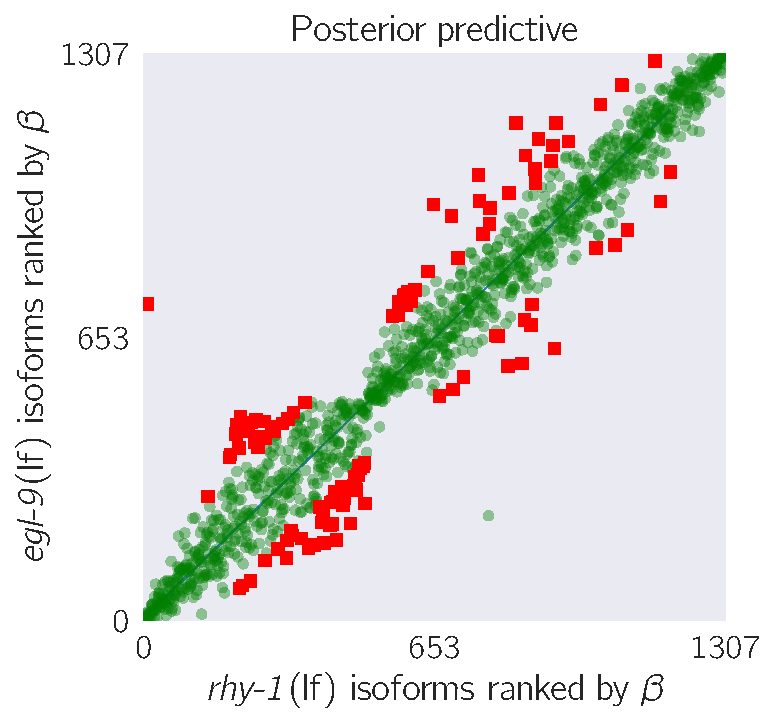
\includegraphics[width=.4\linewidth]{hypims/multiplemodes-eb.pdf}
\caption{
Strong transcriptional correlations can be identified between genes
that share a positive regulatory connection. We took the \egl{} and the \rhy{}
transcriptomes, identified differentially expressed genes common to both
transcriptomes and ranked each gene according to its differential expression
coefficient $\beta$. We plotted the rank of each gene in \rhy{} versus the
rank of the same gene in the \egl{} transcriptome. The result is an almost
perfect correlation. Green, transparent large points mark inliers to the primary
regressions (blue lines); red squares mark outliers to the primary regressions.
}
\label{fig:genetic_interactions}
\end{figure}

We wanted to know whether it was informative to look at quantitative agreement
within STPs. For each mutant pair, we rank-transformed
the regression coefficients $\beta$ of each isoform within the STP, and
calculated lines of best fit using Bayesian regression with a Student-T
distribution to mitigate noise from outliers and plotted the results in a rank plot
(see Fig~\ref{fig:genetic_interactions}). For transcriptomes associated with the
hypoxia pathway, we found that these correlations tended to have
values higher than 0.9 with a tight distribution around the line of best fit.
The correlations for mutants from the hypoxia pathway
with the \fog{} mutant were considerably weaker, with magnitudes between
0.6--0.85 and greater variance around the line of best fit.
Although \gene{hif-1} is known to be genetically repressed by \gene{egl-9}, \gene{rhy-1} and
\gene{vhl-1}~\citep{Epstein2001,Shen2006}, all the correlations
between mutants of these genes and \hif{} were positive.

After we calculated the pairwise correlation within each STP,
we weighted the result of each regression by the
number of isoforms within the STP and
divided by the total number of differentially expressed isoforms present in the
two mutant transcriptomes that contributed to that specific STP,
$N_\mathrm{overlap}/N_{\mathrm{g_1} \cup \mathrm{g2}}$.
The weighted regressions recapitulated a module network (see Fig.~\ref{fig:heatmap}).
We identified a strong positive interaction between \egl{} and \rhy{}.
The magnitude of this weighted correlation derives from the magnitude of the
transcriptomes for these mutants (\egln{} and \rhyn{} differentially expressed
genes respectively) and the overlap between both genes was
extensive, which makes the weighting factor considerably larger than other pairs.
The weak correlation between \hif{} and \egl{} results from the small size of
the \hif{} transcriptome and the small overlap between the transcriptomes.

The fine-grained nature of transcriptional phenotypes means that these weighted
correlations between transcriptomes of single mutants are predictive of genetic
interaction.

% heatmap
\begin{figure}[tbhp]
\centering
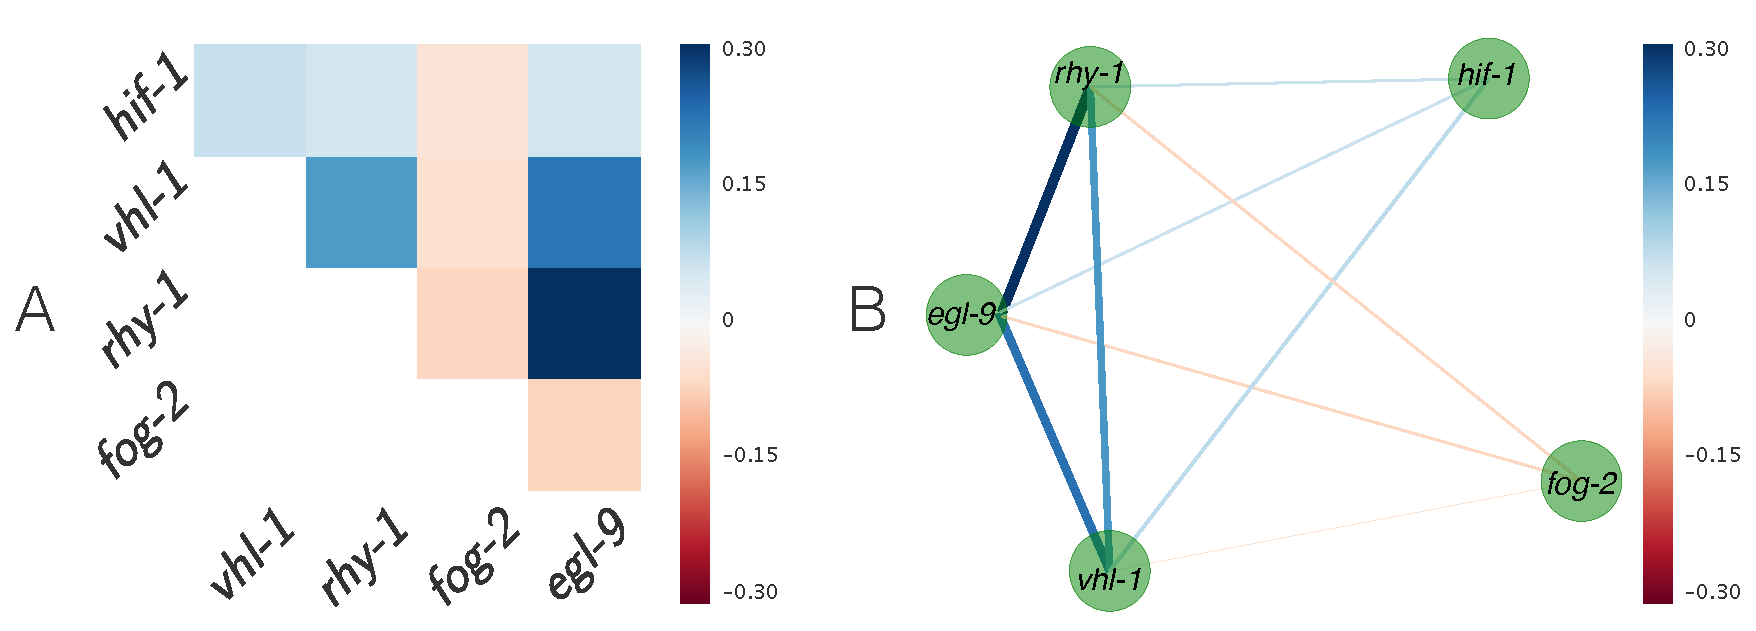
\includegraphics[width=\linewidth]{hypims/bayesian-heatmap-horizontal.pdf}
\caption{
\textbf{A}. Heatmap showing pairwise regression values between all
single mutants. \textbf{B}. Correlation network drawn from \textbf{A}. Edge
width is proportional to the logarithm of the magnitude of the weighted
correlation between two nodes divided by absolute value of the weighted
correlation value of smallest magnitude. Edges are also colored according to the
heatmap in \textbf{A}. Inhibitors of \gene{hif-1} are tightly correlated and form
a control module;
\gene{hif-1} is positively correlated to its inhibitors, albeit weakly;
and
\gene{fog-2}, a gene that is not reported to interact with the hypoxia pathway,
has the smallest, negative correlation to any gene.
}
\label{fig:heatmap}
\end{figure}

\subsubsection*{A quality check of the transcriptomic data reveals excellent agreement
            with the literature}
\label{sub:quality_check}
One way to establish whether genes are acting additively or epistatically to each
other is to perform qPCR of a reporter gene in the single and double mutants. This
approach was used to successfully map the relationships within the hypoxia
pathway (see, for example~\citep{Shao2009,Shen2006}). A commonly used hypoxia reporter
gene is \nhr{}, which is known to exhibit a several-fold increase in mRNA
expression when \hifp{} accumulates~\citep{Shen2006,Shen2005,Park2012}. Likewise,
increased \hifp{} fucntion is known to cause increased of \gene{rhy-1}
and \gene{egl-9}~\citep{Powell-Coffman2010}.

We can
selectively look at the expression of a few genes at a time. Therefore, we
queried the changes in expression of \gene{rhy-1}, \gene{egl-9}, and \nhr{}. We
included the nuclear laminin gene \lam{} as a representative negative control not
believed to be responsive to alterations in the hypoxia pathway.
\nhr{} was upregulated in \egl{}, \rhy{} and \vhl{}, but remains unchanged in \hif{}.
\eglvhl{} had an expression level similar to \egl{}; whereas the
\eglhif{} mutant showed wild-type levels of the reporter expression, as reported
previously~\citep{Shen2006} (see Fig.~\ref{fig:qpcr}).

% in silico qPCR
\begin{figure}[tbhp]
\centering
\includegraphics[width=.5\linewidth]{hypims/qpcr.pdf}
\caption{
\textbf{Top}: Observed $\beta$ values of select genes. We selected
four genes (\gene{rhy-1}, \gene{egl-9}, \nhr{} and \lam{}, shown on the x-axis)
and plotted their regression coefficients, $\beta$, as measured for every
genotype (represented by one of six colors) to study the epistatic relationships
between each gene. Asterisks above a bar represent a regression coefficient
statistically significantly different from 0 (\qval{1}) relative to a wild-type
control. Error bars show standard error of the mean
value of $\beta$. \nhr{} is an expression reporter that has been used previously
to identify \gene{hif-1} regulators~\citep{Shen2006,Shao2009}. \lam{} is shown here
as a negative control that should not be altered by mutations in this pathway.
We measured modest increases in the levels of \gene{rhy-1} mRNA when \hif{} is
knocked out.
}
\label{fig:qpcr}
\end{figure}

We observed changes in \rhy{} expression consistent with previous
literature~\citep{Shen2006} when \hifp{} accumulates.
We also observed increases in \gene{egl-9} expression in \egl{}.
\gene{egl-9} is known as a hypoxia responsive gene~\citep{Powell-Coffman2010}.
Although changes in \gene{egl-9} expression were not statistically significantly
different from the wild-type in
\rhy{} and \vhl{} mutants, the mRNA levels of \gene{egl-9} still trended towards
increased expression in these genotypes.
As with \nhr{}, \gene{egl-9} and \gene{rhy-1} expression were wild-type in
\eglhif{} and \eglvhl{} mutant showed expression phenotypes identical to \egl{}.
This dataset also showed that knockout of \gene{hif-1} resulted in a modest
increase in the levels of \gene{rhy-1}. This suggests that \gene{hif-1}, in
addition to being a positive regulator of \gene{rhy-1}, also inhibits it, which
constitutes a novel observation.
Using a single reporter we would have been able to reconstruct an
important fraction of the genetic relationships between the genes in the hypoxia
pathway–--but would likely fail to observe yet other genetic interactions, such as
the evidence for \gene{hif-1} negatively regulating \gene{rhy-1} transcript levels.


\subsection*{Transcriptome-wide epistasis}
Ideally, any measurement of transcriptome-wide epistasis should conform to certain
expectations. First, it should make use of the regression coefficients of as
many genes as possible. Second, it should be summarizable in a single,
well-defined number. Third, it should have an intuitive behavior, such that
special values of the statistic should each have an unambiguous interpretation.

One way of displaying transcriptome-wide epistasis is to plot transcriptome data onto
an epistasis plot (see Fig~\ref{fig:egl9epistasis}). In an epistasis plot, the
X-axis represents the expected expression of a double mutant $a^-b^-$ if $a$
and $b$ interact additively.
In other words, each individual isoform's x-coordinate is the sum of the regression
coefficients from the single mutants $a^-$ and $b^-$.
The Y-axis represents the deviations from the additive (null) model, and
can be calculated as the difference between the observed regression coefficient
and the predicted regression coefficient. Only genes that are differentially
expressed in all three genotypes are plotted. Assuming that the two genes interact
via a simple phenotype (for example, if both genes affect a transcription factor
that generates the entire transcriptome), these plots will generate specific
patterns that can be described through linear regressions. The slope of these
lines, $s_{a,b}$, is the transcriptome-wide epistasis coefficient.

Epistasis plots can be understood intuitively for simple cases of genetic
interactions. If two genes act additively on the same set of differentially expressed
isoforms then all the plotted points will fall along the line $y=0$.
If two genes interact in an unbranched pathway, then $a^-$ and $b^-$ should
have identical phenotypes for $a^-$, $b^-$ and $a^-b^-$, if all the genotypes are
homozygous for genetic null alleles~\citep{Huang2006}. It follows that the
data points should fall along a line with slope equal to $-\frac{1}{2}$. On the
other hand, in the limit of complete inhibition of $a$ by $b$, the plots should show
a line of best fit with slope equal to $-1$\footnote{Specifically, this follows
from assuming that $b^-$ is wild-type under the conditions assayed; and
$a^-b^-$ = $b^-$ = wild-type}.
Genes that interact synthetically (\emph{i.e.}, through an OR-gate) will fall
along lines with slopes $>0$. When there is epistasis of one gene over another,
the points will fall along a line of best fit with slope $s_{ab=b}$ or $s_{ab=a}$.
This slope must be determined from the single-mutant data.
From this information, we can use the single mutant data to predict the
distribution of slopes that results for each case stated above, as well as for
each epistatic combination ($a^-b^-=a^-$ or $a^-b^-=b^-$). The transcriptome-wide
epistasis coefficient ($s_{a, b}$), emerges as a powerful way to quantify epistasis
because it integrates information from many different genes or isoforms into a
single number (see Fig.~\ref{fig:egl9epistasis}).

In our experiment, we studied two double mutants, \eglhif{} and \eglvhl{}.
We wanted to understand how well an epistasis analysis based on transcriptome-wide
coefficients agreed with the epistasis results reported in the literature, which
were based on qPCR of single genes. Therefore, we performed orthogonal distance
regression on the two gene combinations we studied (\gene{egl-9} and
\gene{vhl-1}; and \gene{egl-9} and \gene{hif-1}) to determine the epistasis
coefficient for each gene pair. We also generated models for the special cases
mentioned above (additivity, $a^-b^-=a^-$, strong suppression, etc\ldots) using
the single mutant data. For every simulation, as well as for the observed data,
we used bootstraps to generate probability distributions of the epistasis
coefficients.

When we compared the predictions for the transcriptome-wide epistasis coefficient,
$s_{egl-9,vhl-1}$ under different assumptions with the observed slope ($-0.42$). We
observed that the predicted slope matched the simulated slope for the case where
\gene{egl-9} is epistatic over \gene{vhl-1} (\egl{} = \eglvhl{}, see
Fig.~\ref{fig:egl9epistasis}) and did not overlap with any other prediction.
Next, we predicted the distribution of $s_{egl-9,hif-1}$ for different pathways
and contrasted with the observed slope. In this case, we saw that the uncertainty
in the observed coefficient overlapped significantly with the strong suppression
model, where \eglp{} strongly suppresses \hifp{}, and also with the model where
\hif{} = \eglhif{}. In this case, both models are reasonable---\hifp{} is strongly
suppressed by \eglp{}, and we know from previous literature that the epistatic
relationship, \hif{} = \eglhif{}, is true for these mutants. In fact, as the
repression of \hifp{} by \eglp{} becomes stronger, the epistatic model should converge
on the limit of strong repression (see
\href{https://wormlabcaltech.github.io/mprsq/analysis_notebooks/epistasis_6.html}
{Epistasis}).

Another way to test which model best explains the epistatic relationship between
\gene{egl-9} and \gene{vhl-1} is to use Bayesian model selection to calculate
an odds ratio between two models to explain the observed data. Models can be placed
into two categories: parameter-free and fit. Parameter free models are `simpler'
because their parameter space is smaller (0 parameters) than the fit models ($n$
parameters). By Occam's razor, simpler models should be preferred to more
complicated models. However, simple models suffer from the drawback that
systematic deviations from them cannot be explained or accomodated, whereas more
complicated models can alter the fit values to maximize their explanatory power.
In this sense, more complicated models should be preferred when the data shows
systematic deviations from the simple model. Odds-ratio selection gives us a way
to quantify the trade-off between simplicity and explanatory power.

We reasoned that comparing a fit model ($y = \alpha\cdot x$, where $\alpha$ is
the slope of best fit) against a parameter-free model ($y = \gamma\cdot x$,
where $\gamma$ is a single number) constituted a conservative approach towards
selecting which theoretical model (if any) best explained the data. In particular,
this approach will tend to strongly favor the line of best fit over simpler model
for all but very small, non-systematic deviations. We decided
that we would reject the theoretical models only if the line of best-fit
was $10^3$ times more likely than the theoretical models (odds ratio, OR $>10^3$).
Comparing the odds-ratio between the line of best fit and the different pathway
models for \gene{egl-9} and \gene{vhl-1} showed similar results to the simulation.
Only the theoretical model \egl{} = \eglvhl{} could not be rejected (OR = 0.46),
whereas all other models were significantly less likely than the line of best fit
(OR $>10^{44}$).
Therefore, \gene{egl-9} is epistatic to \gene{vhl-1}. Moreover,
since $s_{egl-9, vhl-1}$ is strictly between and not equal to $0$ and $-0.5$, we
conclude that \gene{egl-9} acts on its transcriptomic phenotype in
\gene{vhl-1}-dependent and independent manners. A branched pathway that can lead
to epistasis coefficients in this range is a pathway where \gene{egl-9} interacts
with its transcriptomic phenotype via branches that have the same valence (both
positive or both negative)~\citep{Shao2009}. When we performed a similar analysis
to establish the epistatic relationship between \gene{egl-9} and \gene{hif-1},
we observed that the best alternative to a free-fit model was a model where
\gene{hif-1} is epistatic over \gene{egl-9} (OR$=2551$), but the free-fit model
was still preferred. All other models were strongly rejected (OR $>10^{25}$).

% epistasis graph
\begin{figure}[tbhp]
\centering
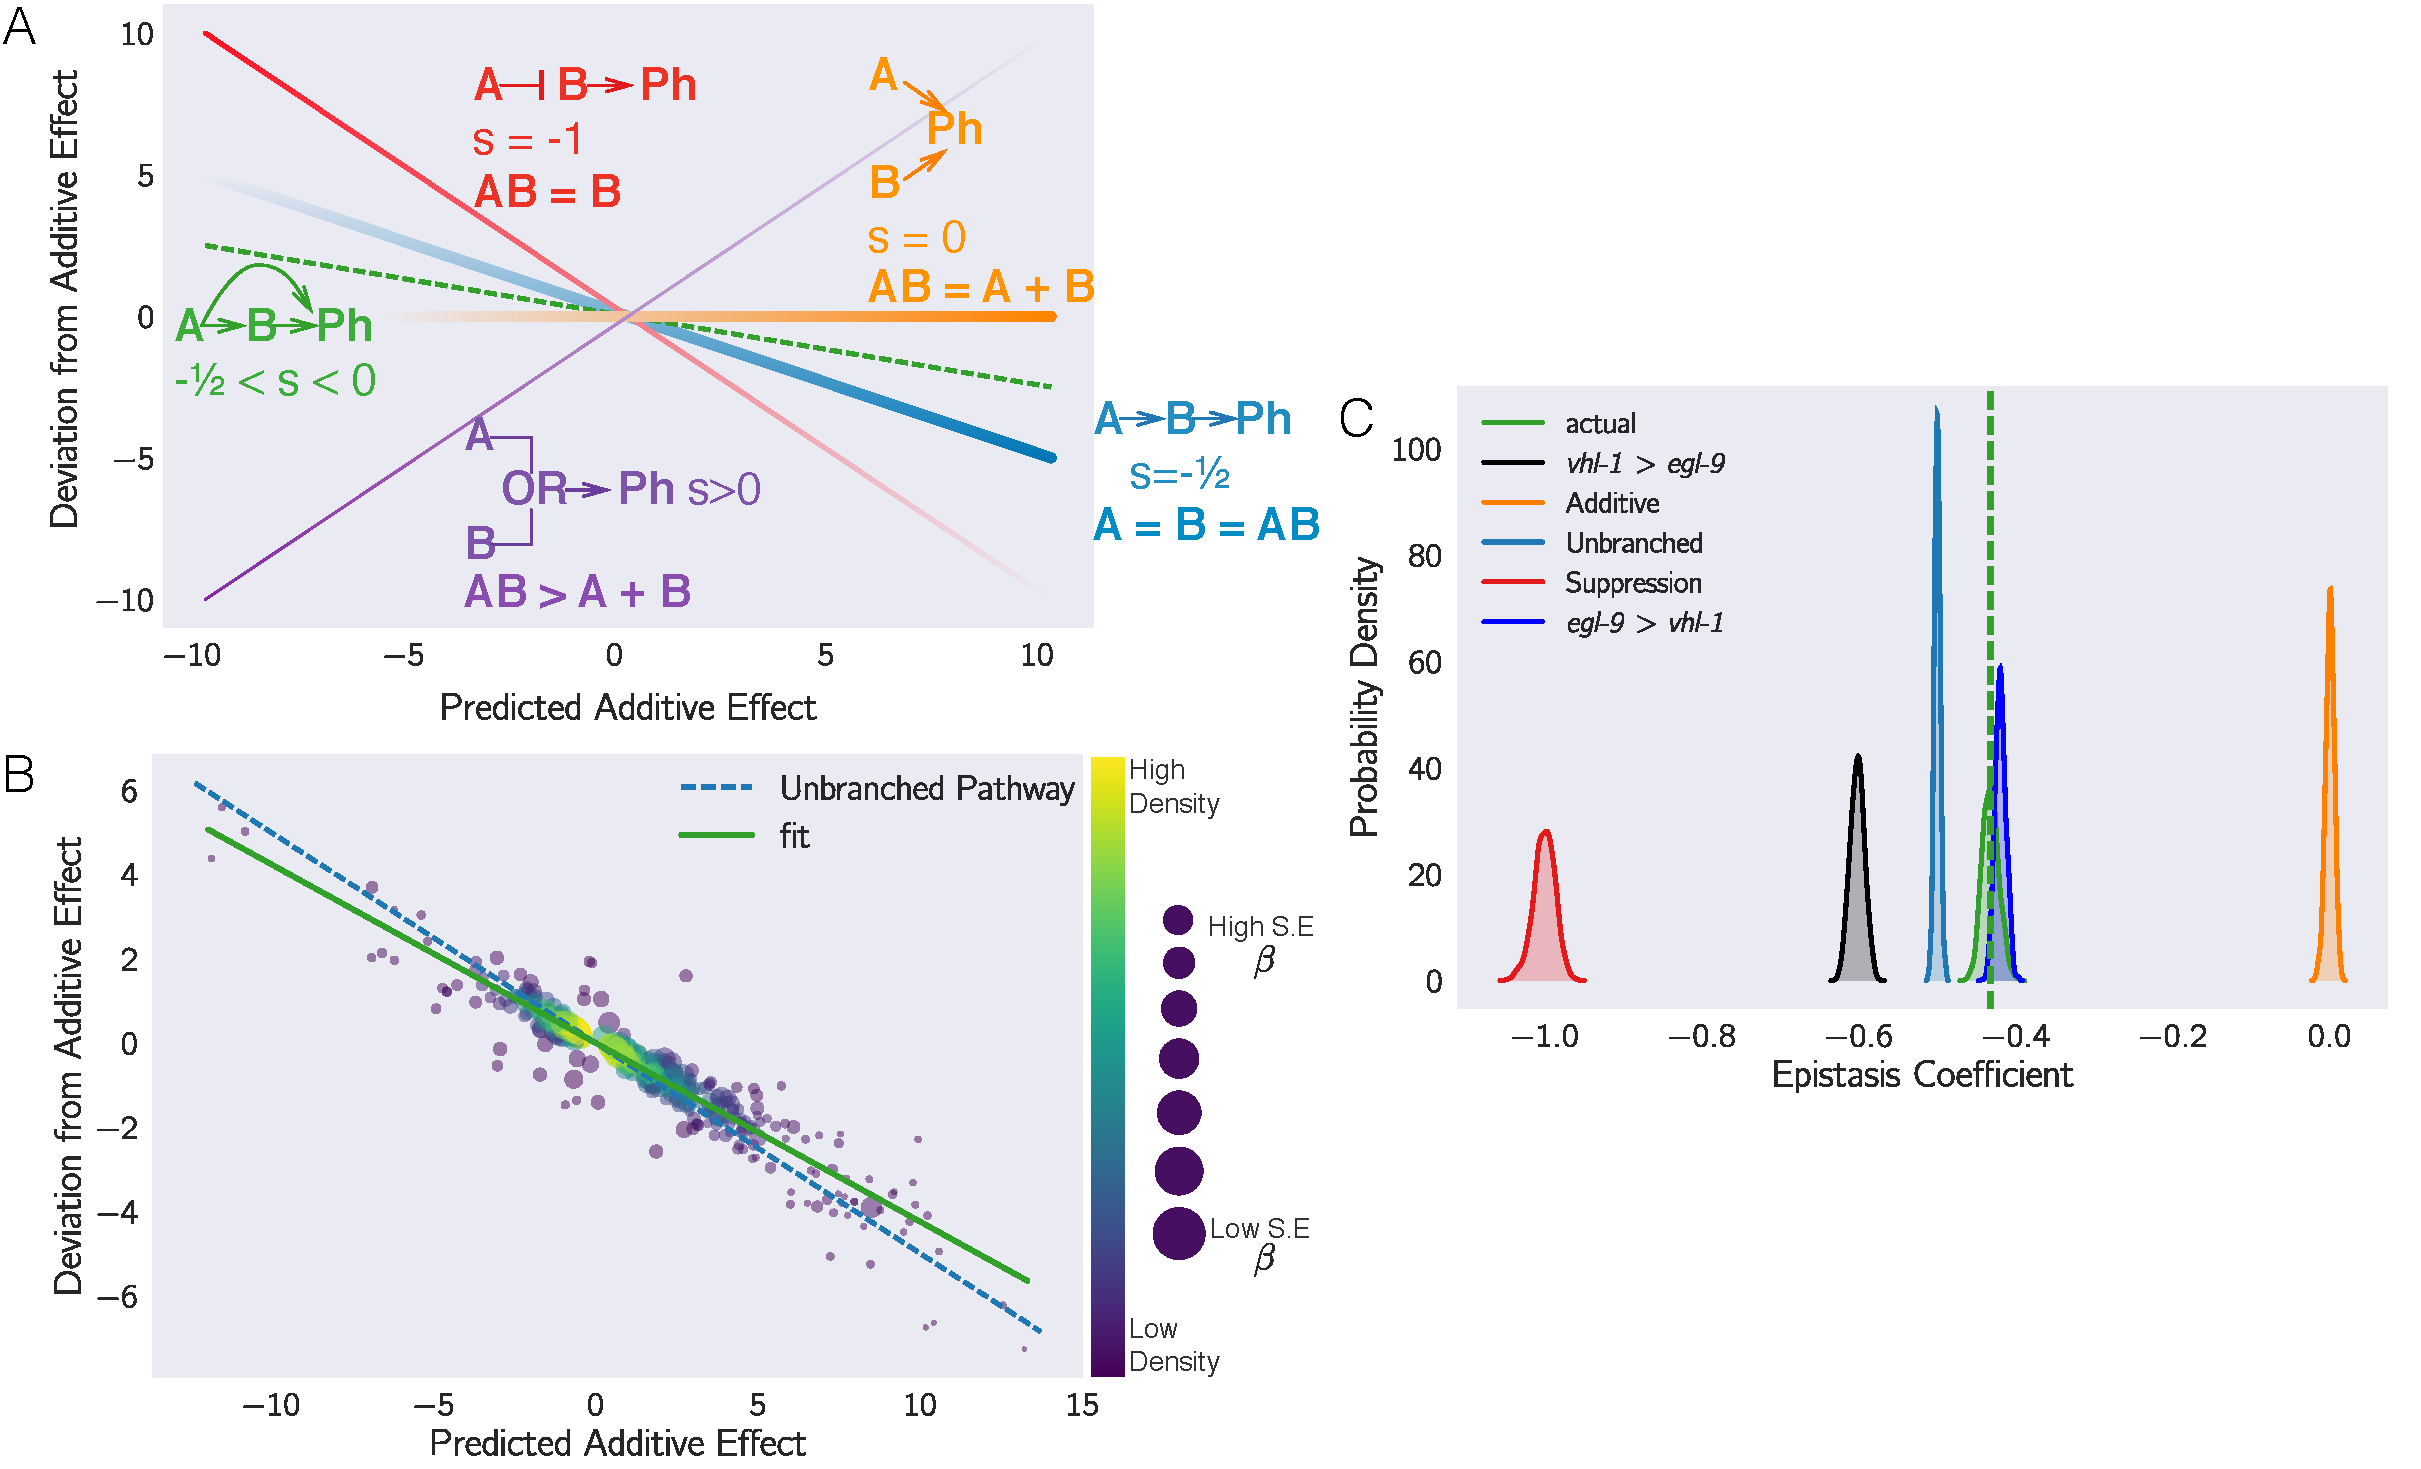
\includegraphics[width=\linewidth]{hypims/egl9hif1-epistasis-horizontal.pdf}
\caption{
(\textbf{A}) Schematic diagram of an epistasis plot. The X-axis on an epistasis
plot is the expected coefficient for a double mutant under an additive model
(null model). The Y-axis plots deviations from this model. Double mutants that
deviate in a systematic manner from the null model exhibit transcriptome-wide epistasis
($s$). To measure $s$, we perform a linear regression on the data. The slope of
the line of best fit is $s$. This coefficient is related to genetic architectures.
Genes that act additively on a phenotype \textbf{(Ph)} will have $s=0$ (orange
line); whereas
genes that act along an unbranched pathway will have $s=-1/2$ (blue line).
Strong
repression is reflected by $s=-1$ (red line). Cases where $s>0$ correspond to
synthetic interactions (purple line), and in the limit as $s\rightarrow\infty$,
the synthetic interaction
must be an OR-gate. Cases where $0 < s < -1/2$ correspond to circuits
that have multiple positive branches; whereas cases where
$-1/2<s< -1$ correspond to cases where the branches have different valence.
Cases where $s < -1$ represent inhibitory branches.
(\textbf{B}) Epistasis plot showing
that the \eglvhl{} transcriptome deviates significantly from a null additive.
Points are colored qualitatively according to density (purple---low,
yellow---high) and size is inversely proportional to the standard
error (S.E.) of the y-axis (larger points, higher accuracy). The purple line
is the line of best fit from an orthogonal distance regression.
(\textbf{C}) Comparison of simulated epistatic coefficients against the observed
coefficient. Green curve shows the bootstrapped observed transcriptome-wide epistasis
coefficient for \gene{egl-9} and \gene{vhl-1}. Dashed green line shows the mean
value of the data. Using the single mutants, we simulated coefficient
distributions for a linear model (light blue, centered at $-0.5$);
an additive model (orange, centered at 0); a model where either
\gene{egl-9} or \gene{vhl-1} masks the other phenotype (dark blue and black,
respectively) and a complete suppression model (red, centered at $-1$).
The observed coefficient overlaps the predicted epistasis curve for
\eglvhl{} = \egl{} (green and dark blue).
}
\label{fig:egl9epistasis}
\end{figure}

\subsubsection*{Epistasis can be predicted}
Given our success in measuring epistasis coefficients, we wanted to know whether
we could predict the epistasis coefficient between \gene{egl-9} and \gene{vhl-1}
in the absence of the \egl{} genotype. Since \rhyp{} indirectly activates
\eglp{}, the \rhy{} transcriptome should contain more or less
equivalent information to the \egl{} transcriptome. Therefore, we generated
predictions of the epistasis coefficient between \gene{egl-9} and \gene{vhl-1}
by substituting in the \rhy{} data. We predicted $s_{rhy-1,vhl-1} = -0.45$.
Similarly, we used the \eglvhl{} double mutant to
measure the epistasis coefficient while replacing the \egl{} dataset with the \rhy{}
dataset. We found that the epistasis coefficient using this substitution was $-0.40$.
This coefficient was different from $-0.50$ (OR $>10^{62}$), reflecting the same
qualitative conclusion that the hypoxia pathway is branched.
In conclusion, we were able to obtain a quantitatively close prediction of the
epistasis coefficient for two mutants using the transcriptome of a related,
upstream mutant. Finally, we showed that in the absence of a single mutant, an
upstream locus can under some circumstances be used to estimate epistasis
between two genes.


\subsection*{Transcriptomic decorrelation can be used to infer functional distance}
\label{sub:decorrelation}
% What are functional interactions?
So far, we have shown that RNA-seq can accurately measure genetic interactions.
However, genetic interactions are far removed from biochemical interactions:
Genetic interactions do not require two gene products to interact physically, nor
even to be physically close to each other. RNA-seq cannot measure physical
interactions between genes, but we wondered whether expression profiling contains
sufficient information to order genes along a pathway.

Single
genes are often regulated by multiple independent sources. The connection between
two nodes can in theory be characterized by the strength of the edges connecting
them (the thickness of the edge); the sources that regulate both
nodes (the fraction of inputs common to both nodes); and the genes that are
regulated by both nodes (the fraction of outputs that are common to both nodes).
In other words, we expected that expression profiles associated with a pathway
would respond quantitatively to quantitative changes in activity of the pathway.
Targeting a pathway at multiple points would lead to expression profile
divergence as we compare nodes that are separated by more degrees of freedom,
reflecting the flux in information between them.

% decorrelation
\begin{figure}[tbhp]
\centering
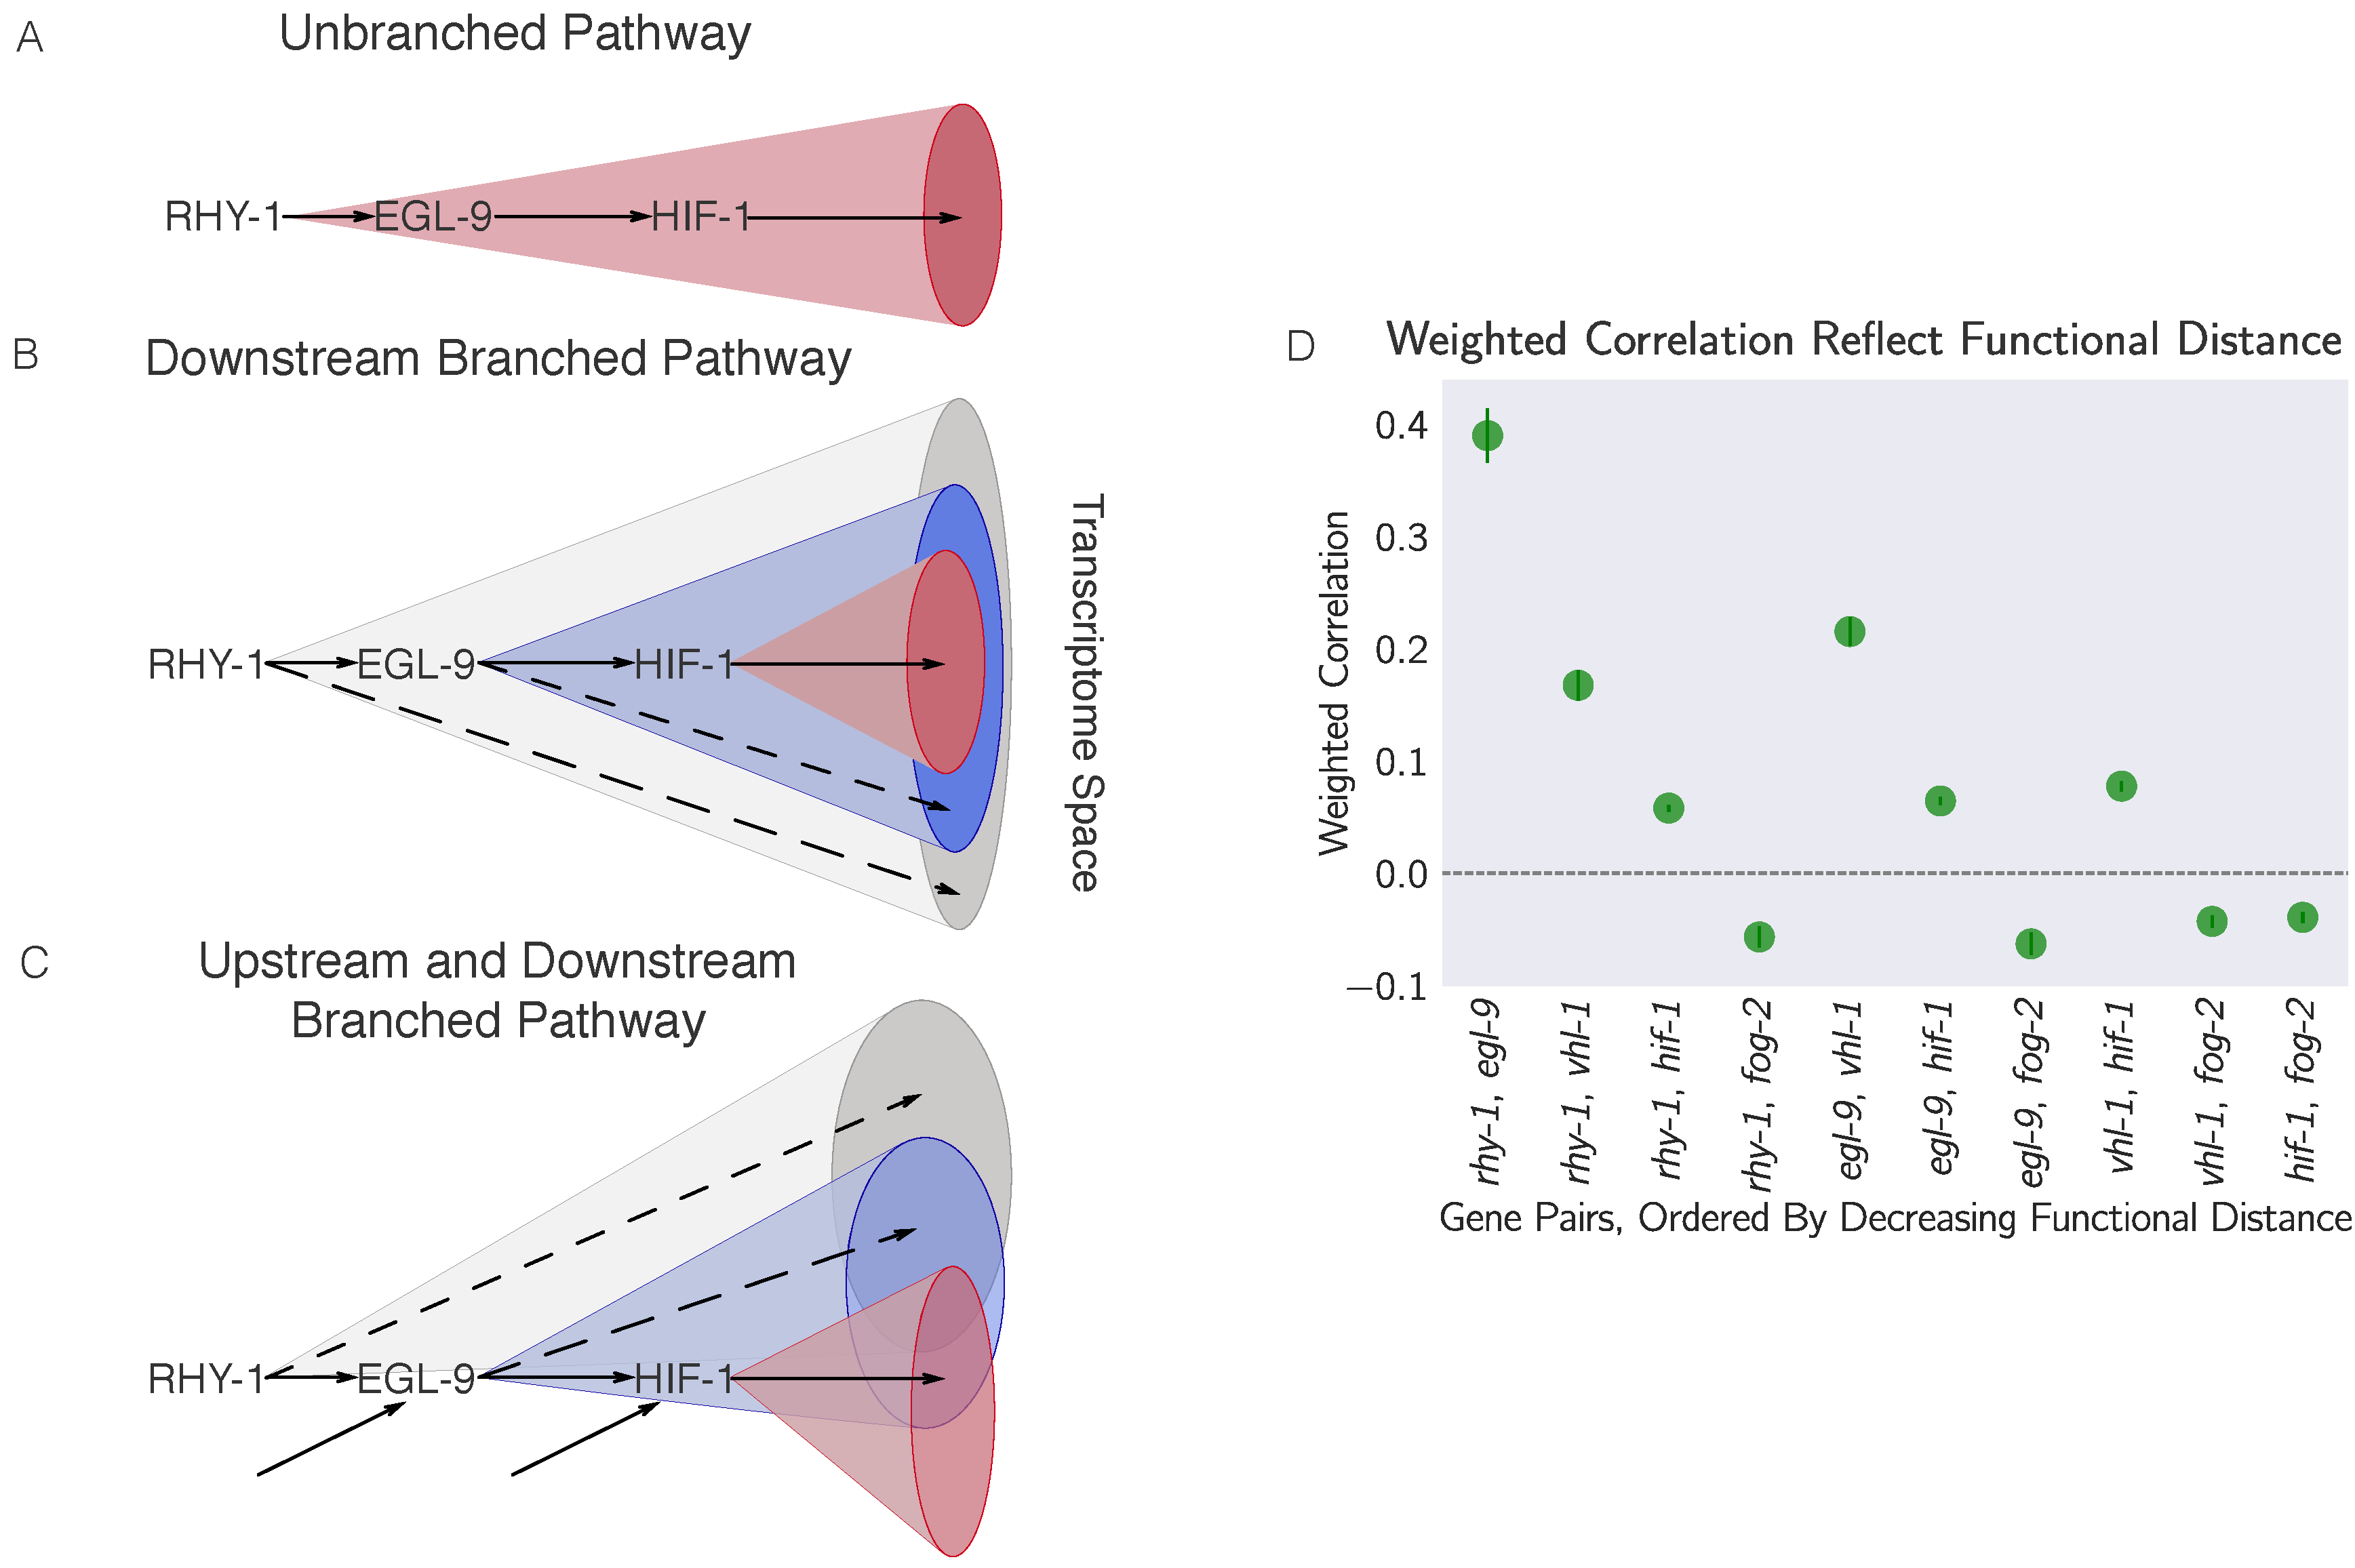
\includegraphics[width=.8\linewidth]{hypims/decorrelation-horizontal.pdf}
\caption{
Theoretically, transcriptomes can be used to order genes in a pathway under
certain assumptions. Arrows in the diagrams above are intended to show the
direction of flow, and do not indicate valence.
\textbf{A}. A linear pathway in which \gene{rhy-1} is the only gene controlling
\gene{egl-9}, which in turn controls \gene{hif-1} does not contain information
to infer the order between genes.
\textbf{B}. If \gene{rhy-1} and \gene{egl-9} have transcriptomic effects that are
separable from \gene{hif-1}, then the \gene{rhy-1} transcriptome should contain
contributions from \gene{egl-9}, \gene{hif-1} and \gene{egl-9}- and
\gene{hif-1}-independent pathways. This pathway contains enough information to
infer order.
\textbf{C}. If a pathway is branched both upstream and downstream,
transcriptomes will show even faster decorrelation. Nodes that are
separated by many edges may begin to behave almost independently of each other
with marginal transcriptomic overlap or correlation.
\textbf{D}. The hypoxia pathway can be ordered.
We hypothesize the rapid decay in correlation is due to a mixture of
upstream and downstream branching that happens along this pathway. Bars show the
standard error of the weighted coefficient from the Monte Carlo Markov Chain
computations.
}
\label{fig:decorrelation}
\end{figure}


We investigated the possibility that transcriptomic signals do in fact contain
relevant information about the degrees of separation by weighting the robust
Bayesian regression between each pair of genotypes by the size of the shared
transcriptomic phenotype of each pair divided by the total number of isoforms
differentially expressed in either mutant
($N_\mathrm{Intersection}/N_{\mathrm{Union}}$). We plotted the weighted
correlation of each gene pair, ordered by increasing functional distance
(see Fig.~\ref{fig:decorrelation}). In every case, we see that the weighted
correlation decreases monotonically due mainly, but not exclusively, to a smaller
STP.\@ We believe that this result is not due to random noise or insufficiently
deep sequencing. Instead, we propose a framework in which every gene is regulated
by multiple different molecular species, which induces progressive decorrelation.
This decorrelation in turn has two consequences. First, decorrelation within a
pathway implies that two nodes may be almost independent of each other if the
functional distance between them is large. Second, it may be possible to use
decorrelation dynamics to infer gene order in a branching pathway, as we have
done with the hypoxia pathway.

\subsection*{The circuit topology of the hypoxia pathway explains patterns in
            the data}
\label{sub:topology}
We noticed that while some of the rank plots contained a clear positive correlation
(see Fig.~\ref{fig:genetic_interactions}), other rank plots showed
a discernible cross-pattern (see Fig.~\ref{fig:xpattern}). In particular, this
cross-pattern emerged between \vhl{} and \rhy{} or between \vhl{} and \egl{},
even though genetically \gene{vhl-1}, \gene{rhy-1} and \gene{egl-9} are all
inhibitors of \hif{}. Such cross-patterns could be indicative of feedback loops
or other complex interaction patterns.

% correlative genetics again
\begin{figure}[tbhp]
\centering
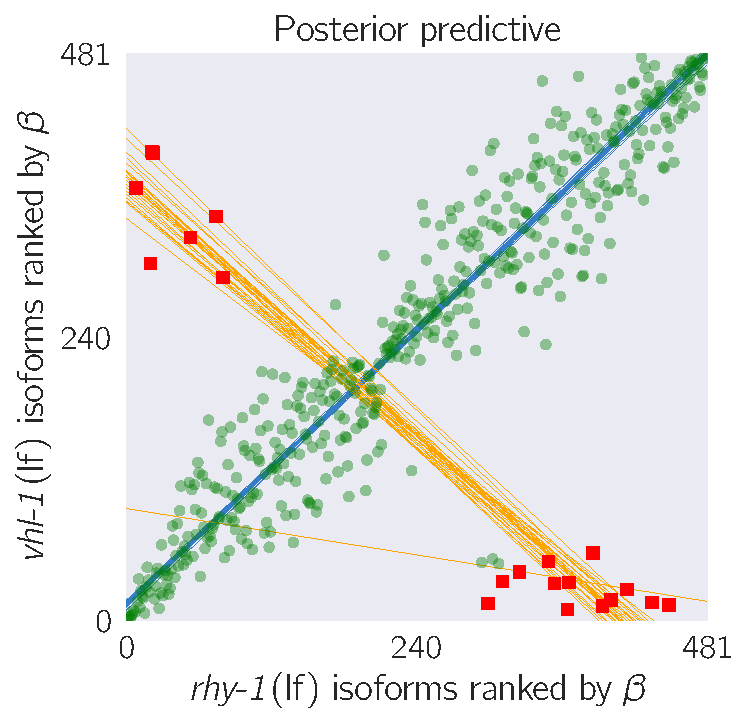
\includegraphics[width=.4\linewidth]{hypims/multiplemodes-ed.pdf}
\caption{
A feedback loop can generate transcriptomes that are both
correlated and anti-correlated. The \vhl{}/\rhy{} STP shows a cross-pattern.
Green large points are inliers to the first
regression. Red squares are outliers to the first regression. Only the red
small points were used for the secondary regression. Blue lines are representative
samples of the primary bootstrapped regression lines. Orange lines are
representative samples of the secondary bootstrapped regression lines.
}
\label{fig:xpattern}
\end{figure}



If the above is correct, then it should be possible to identify
\gene{egl-9}-independent, \rhy{}-dependent target genes in a
logically consistent way.
One erroneous way to identify these targets is via
subtractive logic. Using subtractive logic, we would identify genes that are
differentially expressed in \rhy{} mutants but not in \egl{} mutants.  Such a
gene set would
consist of almost 700 genes. One major drawback of subtractive logic is that it
cannot be applied when feedback loops exist between the genes in question.
Another problem is that the set of identified genes are statistically indistinguishable
from false positive and false negative hits because they have no distinguishing
property beyond the condition that they should be differentially expressed in
one mutant but not the other. In fact, this is exactly the behavior expected of
false-positive or false-negative hits---presence in one, but not multiple, mutants.
We need to consider the relationship between two genes before we can begin to
identify targets which expression is dependent on one gene and independent
of the other.

\gene{rhy-1} and \gene{egl-9} share a well-defined relationship. \rhyp{}
inhibits \cyslp{},
which in turn inhibits \eglp{}~\citep{Ma2012}. Therefore, loss of \rhyp{} leads
to inactivation of \eglp{}, which leads to increase in the cellular levels of
\hifp{}. \hifp{} in turn causes the mRNA levels of \gene{rhy-1} and \gene{egl-9}
to increase,
as they are involved in the \gene{hif-1}-dependent hypoxia response. However, since
\gene{rhy-1} has been mutated, the observed transcriptome is
\rhyp{} `null'; \eglp{} `null'; \hifp{} `on'. The situation is similar for
\egl{}, except that \rhyp{}
is not inactive, and therefore the observed transcriptome is the result of
\rhyp{} `up'; \eglp{} `null'; and \hifp{} `on'. From this pattern, we conclude that
the \egl{} and \rhy{} transcriptomes should exhibit a cross-pattern when plotted
against each other: The positive
arm of the cross is the result of the \eglp{} `null'; \hifp{} `on' dynamics; and the
negative arm reflects the different direction of \rhyp{} activity between
transcriptomes. No negative arm is visible (with the exception of two
outliers, which are annotated as pseudogenes in WormBase). Therefore, in this
dataset we do not find genes that have \gene{egl-9} independent,
\gene{rhy-1}-dependent expression patterns.

We also identified a main hypoxia response induced by disinhibiting
\gene{hif-1} (355 genes) by identifying genes that were commonly up-regulated
amongst \egl{}, \rhy{} and \vhl{} mutants. Although the hypoxic response is likely
to involve between three and seven times more genes (assuming the \rhy{} transcriptome
reflects the maximal hypoxic response), this is a conservative
estimate that minimizes false positive results, since these changes were
identified in four different genotypes with three replicates each. This response
included five transcription factors (\gene{W02D7.6}, \nhr{}, \gene{ztf-18},
\gene{nhr-135} and \gene{dmd-9}). The full list of genes associated with the
hypoxia response can be found in the Supplementary Table 1.
% TODO: SI numbering

\gene{hif-1}-independent effects of \gene{egl-9} have been reported
previously~\citep{Park2012}, which led us to question whether we could identify
similar effects in our dataset. We have observed that \hif{} displays a modest
increase in the transcription of \gene{rhy-1}, from which we speculated that
\eglp{} would have increased activity in the \hif{} mutant compared to the wild-type.
Therefore, we searched for genes that were regulated in an opposite manner between
\hif{} and \eglhif{}, and that were regulated in the same direction between
all \egl{} genotypes. We did not find any genes that met these conditions.

We also searched for genes with \gene{hif-1} independent, \gene{vhl-1}-dependent gene
expression and found \vhltargets{} genes, which can be found in the Supplementary
Table 2.
Finally, we searched for candidates directly regulated by \gene{hif-1}. Initially, we
searched for genes that had were significantly altered in \hif{} genotypes in one
direction, but altered in the opposite direction in mutants that activate the
\hifp{} response. Only two genes (\emph{R08E5.3}, and \emph{nit-1}) met these
conditions. This could reflect the fact that \hifp{} exists at very low
levels in \cel{}, so loss of function mutations in \gene{hif-1} might only have
mild effects on its transcriptional targets. We reasoned that genes
that are overexpressed in mutants that induce the \hifp{} response would be enriched
for genes that are direct candidates.  We found \hiftargets{}  genes which have
consistently increased expression in mutants with a constitutive hypoxic response.
These genes can be found in the Supplementary Table 3.


\subsubsection*{Enrichment analysis of the hypoxia response}
\label{sub:ea_hypoxia}
To validate that our transcriptomes were correct, and to understand how
functionalities may vary between them, we subjected each decoupled response to
enrichment analysis using the WormBase Enrichment Suite~\citep{Angeles-Albores2016,
Angeles-Albores2016b}.

\begin{figure}[tbhp]
\centering
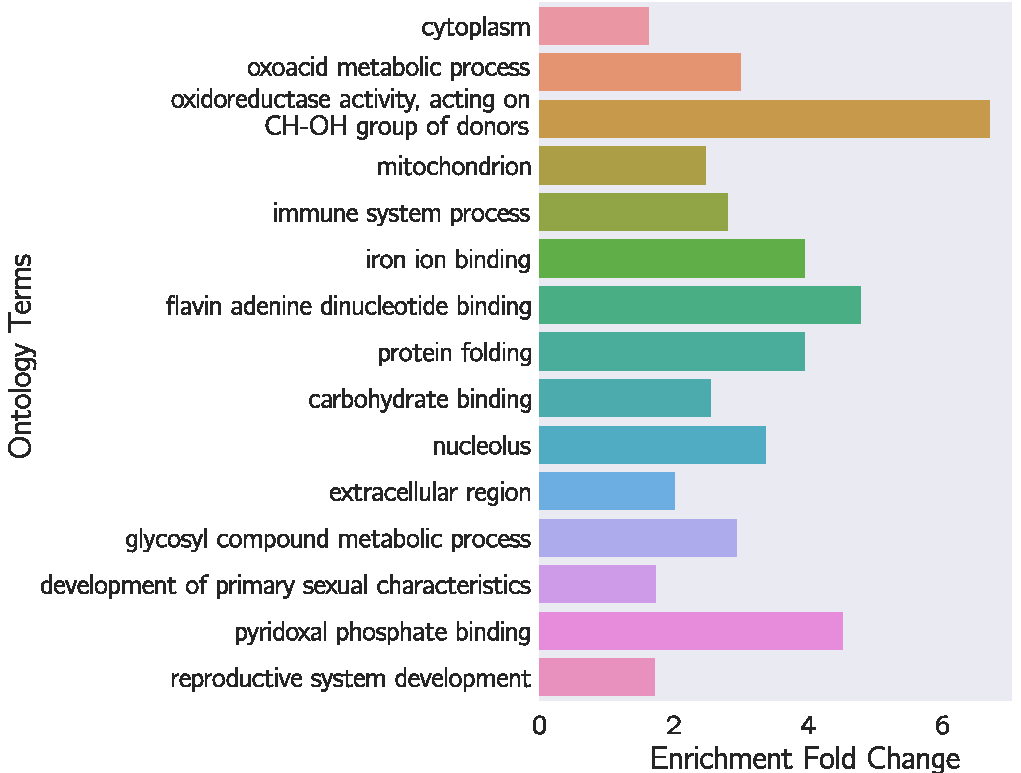
\includegraphics[width=.7\linewidth]{hypims/hypoxia_response_gea.pdf}
\caption{
Gene ontology enrichment analysis of genes associated with the main hypoxia response.
A number of terms reflecting catabolism and bioenergetics are enriched.
}
\label{fig:hyp_gea}
\end{figure}

We used gene ontology enrichment analysis (GEA) on the main hypoxia response program.
This showed that the terms `oxoacid metabolic process' (\qval{4}, 3.0 fold-change,
24 genes), `iron ion binding' (\qval{2}, 3.8 fold-change, 10 genes), and `immune
system process' (\qval{3}, 2.9 fold-change, 20 genes) were significantly enriched.
GEA also showed enrichment of the term `mitochondrion' (\qval{3}, 2.5 fold-change,
29 genes) (see Fig.~\ref{fig:hyp_gea}). Indeed, \hif{} has been implicated in
all of these biological and molecular functions~\citep{Luhachack2012,Ackerman2012,
Romney2011,Semenza2011}.
As benchmark on the quality of our data, we selected a set of 22 genes known to
be responsive to \hifp{} levels from the literature and asked whether these genes
were present in our hypoxia response list. We found $8/22$ known genes, which
constitutes a statistically significant result ($p<10^{10}$). The small number of
reporters found in this list probably reflects the conservative nature of our
estimates.
We studied the \gene{hif-1}-independent, \gene{vhl-1}-dependent gene set
using enrichment analysis but no terms were significantly enriched.

\subsection*{Identification of non-classical epistatic interactions}
\label{sub:hifoh}
\hif{} has traditionally been viewed as existing in a genetic OFF state under
normoxic conditions. However, our dataset indicates that \hifn{} genes show
altered expression when \gene{hif-1} function is removed in normoxic conditions.
Moreover, we observed positive correlations between \hif{} $\beta$ coefficients
and \egl{}, \vhl{} and \rhy{} $\beta$ coefficients in spite of the negative
regulatory relationships between these genes and \gene{hif-1}. Such
positive correlations could indicate a different relationship between these genes
than has previously been reported, so we attempted to substantiate them through
epistasis analyses.

To perform epistasis analyses, we first identified genes that exhibited violations
of the canonical genetic model of the hypoxia pathway. To this end, we searched for
genes that exhibited different behaviors between \egl{} and \vhl{}, or
between \rhy{} and \vhl{} (we assume that all results from the
\rhy{} transcriptome reflect a complete loss of \gene{egl-9} activity). We found
\hifohtargets{} that satisfied this condition (see Fig.~\ref{fig:hif1oh},
Supplemental Table 4).
Additionally, many of these genes exhibited a new kind of epistasis. Namely,
\gene{egl-9} was epistatic over \gene{vhl-1}. Identification of a set of genes
that have a consistent set of relationships between themselves suggests that
we have identified a new aspect of the hypoxia pathway.

\begin{figure}[tbhp]
\centering
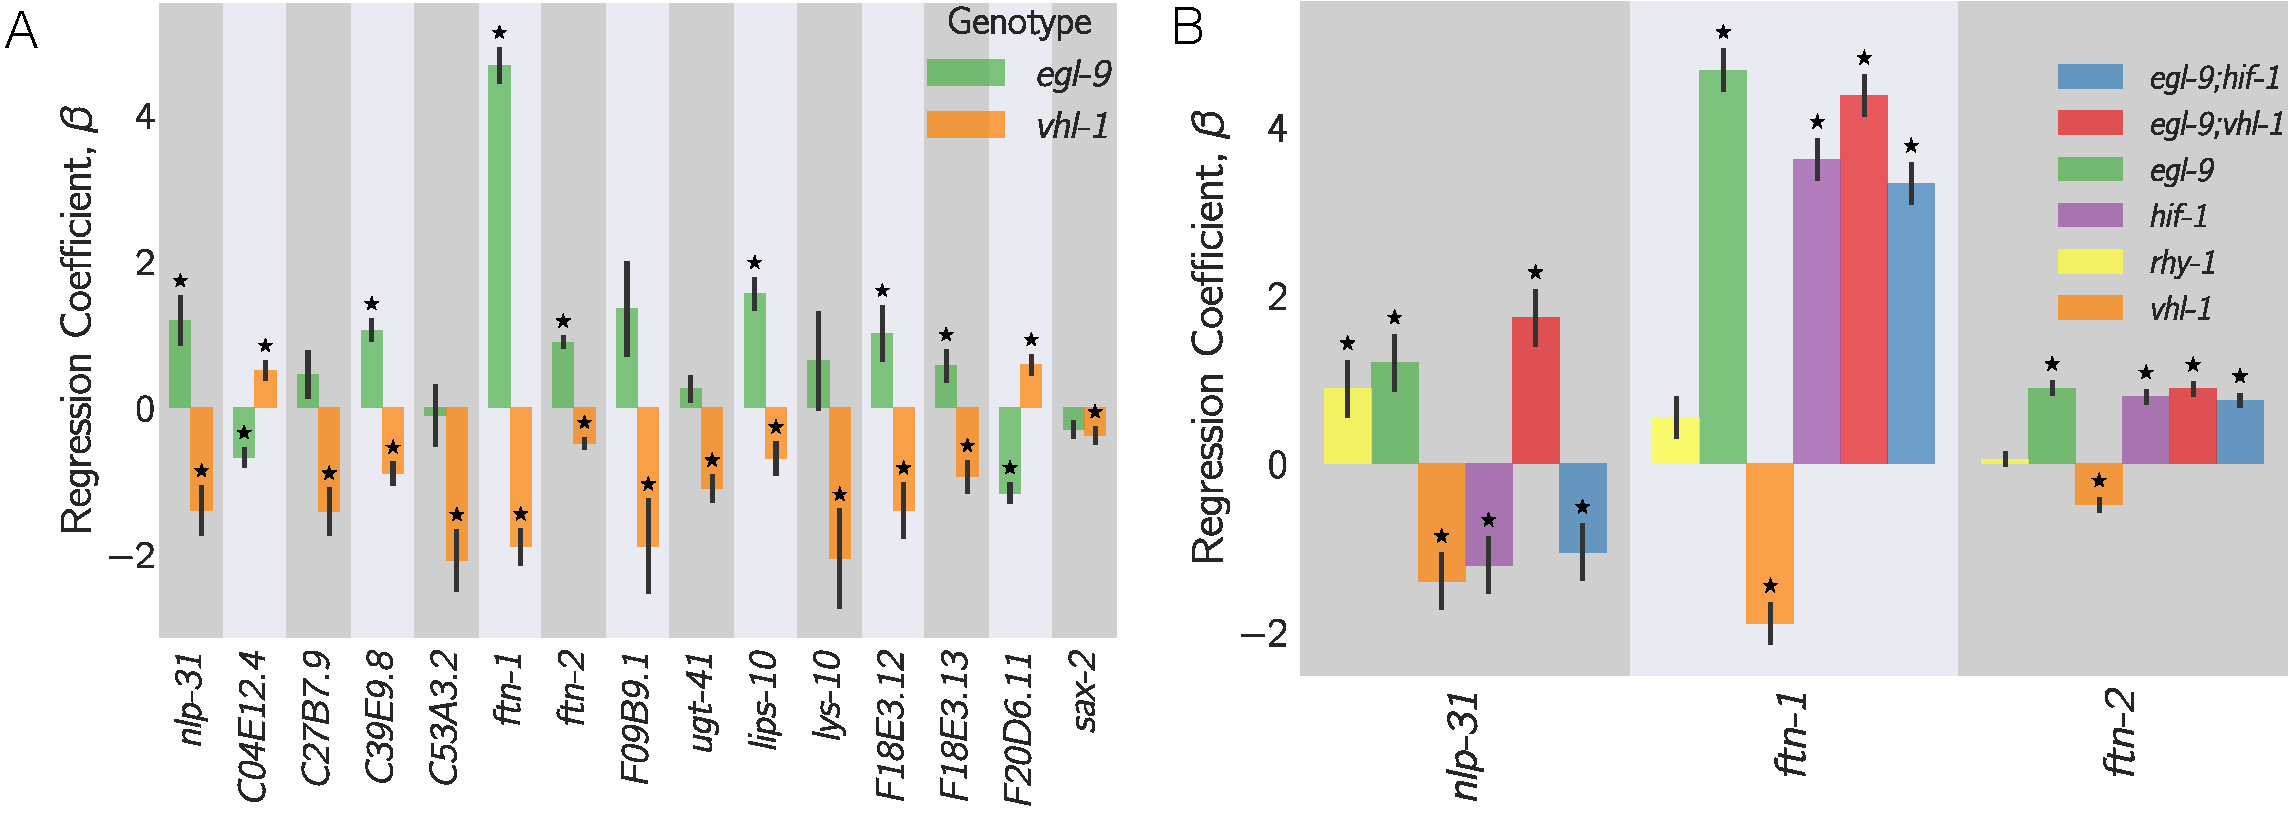
\includegraphics[width=\linewidth]{hypims/hif1oh-epistasis-horizontal.pdf}
\caption{
\textbf{A}. 27 genes in \cel{} exhibit non-classical epistasis in the hypoxia
pathway, characterized by opposite effects on gene expression, relative to the
wild-type, of of the \vhl{} compared to \egl{} (or
\rhy{}) mutants. Shown are a random selection of 15 the 27 genes for illustrative
purposes.
\textbf{B}. Representative genes showing that non-canonical epistasis shows a
consistent pattern. \vhl{} mutants have an opposite effect to \egl{}, but
\gene{egl-9} remains epistatic to \gene{vhl-1} and loss-of-function mutations in
\gene{hif-1} suppress the \egl{} phenotype. Asterisks show $\beta$ values
significantly different from 0 relative to wild-type (\qval{1}).
}
\label{fig:hif1oh}
\end{figure}

To illustrate this, we focused on three genes, \nlp{}, \ftna{} and \ftnb{}, which
epistasis patterns that we felt reflected the population well. \ftna{} and \ftnb{}
are both described in the literature as genes that are responsive to mutations in
the hypoxia pathway. Moreover, these genes have been previously described to have
aberrant behaviors~\citep{Ackerman2012,Romney2011}, specifically the
opposite effects of \egl{} and \vhl{}. These studies showed that loss of \vhl{}
decreases expression of \ftna{} and \ftnb{} using both RNAi and alleles, which
allays concerns of strain-specific interference. Moreover, Ackerman and Gems (2012)
showed that \gene{vhl-1} is epistatic to \gene{hif-1} for the \ftna{}
expression phenotype, and that loss of
\hifp{} is associated with increased expression of \ftna{} and \ftnb{}. We observed
that \gene{hif-1} was epistatic to \gene{egl-9}, and that \gene{egl-9} and
\gene{hif-1} both promoted \ftna{} and \ftnb{} expression.

Epistasis analysis of \ftna{} and \ftnb{} expression reveals that \gene{egl-9} is
epistatic to \gene{hif-1}; that \gene{vhl-1} has opposite effects to \gene{egl-9},
and that \gene{vhl-1} is epistatic to \gene{egl-9}. Analysis of \nlp{}
reveals similar relationships. \nlp{} expression is decreased in \hif{},
and increased in \egl{}. However, \gene{egl-9} is epistatic to \gene{hif-1}.
Like \ftna{} and \ftnb{}, \gene{vhl-1} has the opposite effect to \gene{egl-9},
yet is epistatic to \gene{egl-9}. We propose in the Discussion a model for how
\hifp{} might regulate these targets.

\subsection*{\hifp{} in the cellular context}
\label{sub:metabolism}

We identified the transcriptional changes
associated with bioenergetic pathways in \cel{} by extracting from
WormBase all genes associated with the tricarboxylic acid (TCA) cycle, the
electron transport chain (ETC) and with the \cel{} GO term energy reserve.
Previous research has described the effects of mitochondrial dysfunction in
eliciting the hypoxia response~\citep{Lee2010}, but transcriptional feedback
from \hifp{} into bioenergetic pathways has not been as extensively in \cel{},
as in vertebrates (see, for example~\citep{Semenza1994,Semenza2012}).
We also searched for the changes in ribosomal components and the proteasome, as
well as for terms relating to immune response (see Fig~\ref{fig:genomewide}).

\begin{figure}[tbhp]
\centering
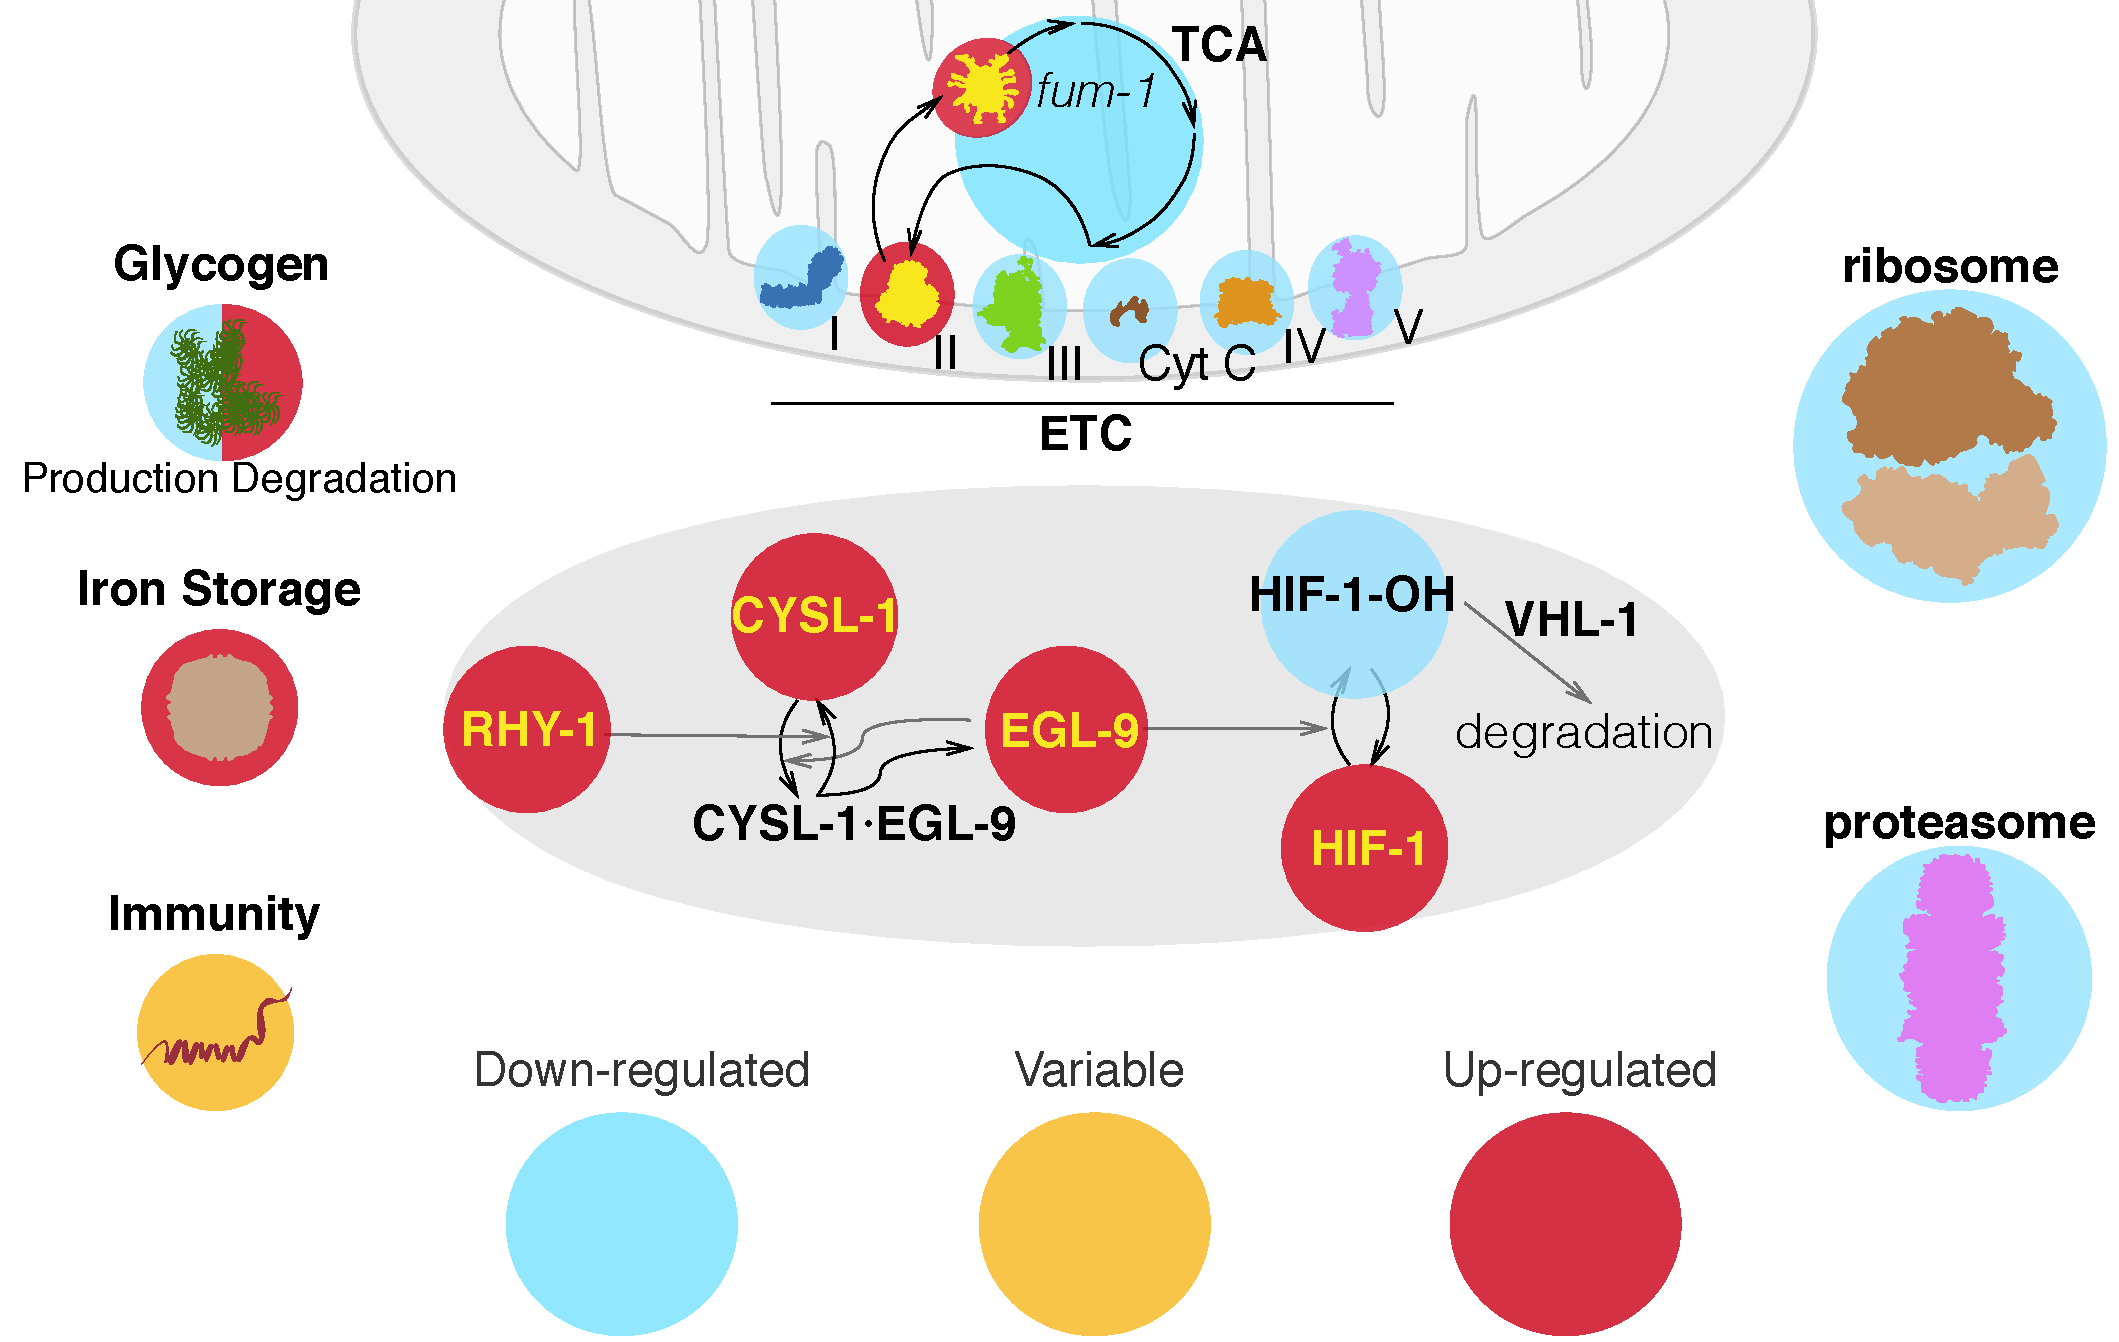
\includegraphics[width=.7\linewidth]{hypims/hif1genomewide.pdf}
\caption{
A graphic summary of the genome-wide effects of \hifp{} from our RNA-seq data.
}
\label{fig:genomewide}
\end{figure}

\subsubsection*{Bioenergetic pathways}
Our data shows that most of the enzymes involved in the TCA cycle and in the ETC
are down-regulated when \hifp{} is induced in agreement with the previous
literature~\citep{Semenza2012}.
However, the fumarase gene \gene{fum-1} and the mitochondrial complex II stood out
as notable exceptions to the trend, as they were up-regulated in every single
genotype that causes deployment of the hypoxia response. FUM-1 catalyzes the
reaction of fumarate into malate, and complex II catalyzes the reaction of
succinate into fumarate. Complex II has been identified as a source of reserve
respiratory capacity in neonatal rat cardiomyocytes previously~\citep{Pfleger2015}.
We found two energy reserve genes that were down-regulated by \hifp{}.
\gene{aagr-1} and \gene{aagr-2}, which are predicted to function in glycogen
catabolism~\citep{Sikora2010}.
Three distinct genes involved in energy reserve were up-regulated. These genes were
\gene{ogt-1}, which encodes O-linked GlcNac Transferase gene; \gene{T04A8.7},
encoding an ortholog of human glucosidase, acid beta (GBA); and \gene{T22F3.3},
encoding ortholog of human glycogen phosphorylase isozyme in the muscle (PYGM).

\subsubsection*{Protein synthesis and degradation}
\hif{} is also known to inhibit protein synthesis and translation in varied
ways.~\citep{Brugarolas2004}. Most reported effects of
\hifp{} on the translation machinery are posttranslational, and no reports to date
show transcriptional control of the ribosomal machinery in \cel{} by \hifp{}. We
used the WormBase Enrichment Suite Gene Ontology
dictionary~\citep{Angeles-Albores2016b} to extract 143 protein-coding genes
annotated as `structural constituents of the ribosome' and we queried whether
they were differentially expressed in our mutants. \egl{}, \vhl{}, \rhy{} and
\egl{};\vhl{} showed differential expression of 91 distinct ribosomal constituents
(not all constituents were detected in all genotypes). For every one of these
genotypes, these genes were always down-regulated. In contrast, \hif{} showed
up-regulation of a single ribosomal constituent.

Next, we asked whether \hifp{} has any transcriptional effects on the
proteasomal constituents; no such effects of \hifp{} on the proteasome
have been reported in \cel{}. Out of 40 WormBase-annotated proteasomal constituents,
we found 31 constituents that were differentially expressed in at least one of the
four genotypes that induce a hypoxic response. Every gene we found was down-regulated
in at least two out of the four genotypes we studied.

\section*{Discussion}
\subsection*{The \cel{} hypoxia pathway can be reconstructed entirely from
             RNA-seq data}
In this paper, we have shown that whole-organism transcriptomic phenotypes
can be used to reconstruct genetic pathways and to discern previously overlooked
or uncharacterized genetic interactions. We successfully reconstructed the hypoxia
pathway, and inferred order of action (\gene{rhy-1} activates \gene{egl-9},
\gene{egl-9} and \gene{vhl-1} inhibit \gene{hif-1}), and we were able to infer
from transcriptome-wide epistasis measurements that \gene{egl-9} exerts
\gene{vhl-1}-dependent and independent inhibition on \gene{hif-1}.

\subsection*{\hifp{} and the cellular environment}

In addition to reconstructing the pathway, our dataset allowed us
to observe a wide variety of physiologic changes that occur as a result of the
\hifp{}-dependent hypoxia response. In particular, we observed down-regulation of most
components of the TCA cycle and the mitochondrial electron transport chain with
the exceptions of \gene{fum-1} and the mitochondrial complex II.\@ The mitochondrial
complex II catalyzes the reaction of succinate into fumarate.
In mouse embryonic fibroblasts, fumarate has been
shown to antagonize \hifp{} prolyl hydroxylase domain (PHD) enzymes, which are
orthologs of \eglp{}~\citep{Sudarshan2009}.
If the inhibitory role of fumarate on PHD enzymes is conserved in \cel{},
upregulation of complex II by \hifp{} during hypoxia may increase
intracellular levels of fumarate, which in turn could lead to artificially high
levels of \hifp{}
even after normoxia resumes. The increase in fumarate produced by the complex
could be compensated by increasing expression of \gene{fum-1}. Increased fumarate
degradation allows \cel{} to maintain plasticity in the hypoxia pathway, keeping
the pathway sensitive to oxygen levels.

\subsection*{Interpretation of the non-classical epistasis in the hypoxia pathway}
The observation of almost 30 genes that exhibit a specific pattern of non-classical
epistasis suggests the existence of previously undescribed aspects of the hypoxia
pathway. Some of these non-classical epistases had been observed
previously~\citep{Ackerman2012,Romney2011,Luhachack2012}, but
no satisfactory mechanism has been proposed to explain this biology.
\citet{Romney2011} and \citet{Ackerman2012}
suggest that \hifp{} integrates information on iron concentration in the
cell to bind to the \ftna{} promoter, but could not definitively establish
a mechanism.
It is unclear why deletion of \gene{hif-1} induces \ftna{}
expression, deletion of \gene{egl-9} also causes induction of \ftna{} expression,
but deletion of \gene{vhl-1} removes this inhibition. Moreover, \citet{Luhachack2012}
have previously reported that certain genes important for the \cel{} immune response
against pathogens reflect similar expression patterns. Their interpretation
was that \gene{swan-1}, which encodes a binding partner to \eglp{}~\citep{Shao2010},
is important for modulating \hifp{} activity in some manner. The lack of a
conclusive double mutant analysis in this work means the role of SWAN-1 in
modulation of \hifp{} activity remains to be demonstrated. Nevertheless, mechanisms
that call for additional transcriptional modulators become less likely given the
number of genes with different biological functions that exhibit the same pattern.

\begin{figure}[tbhp]
\centering
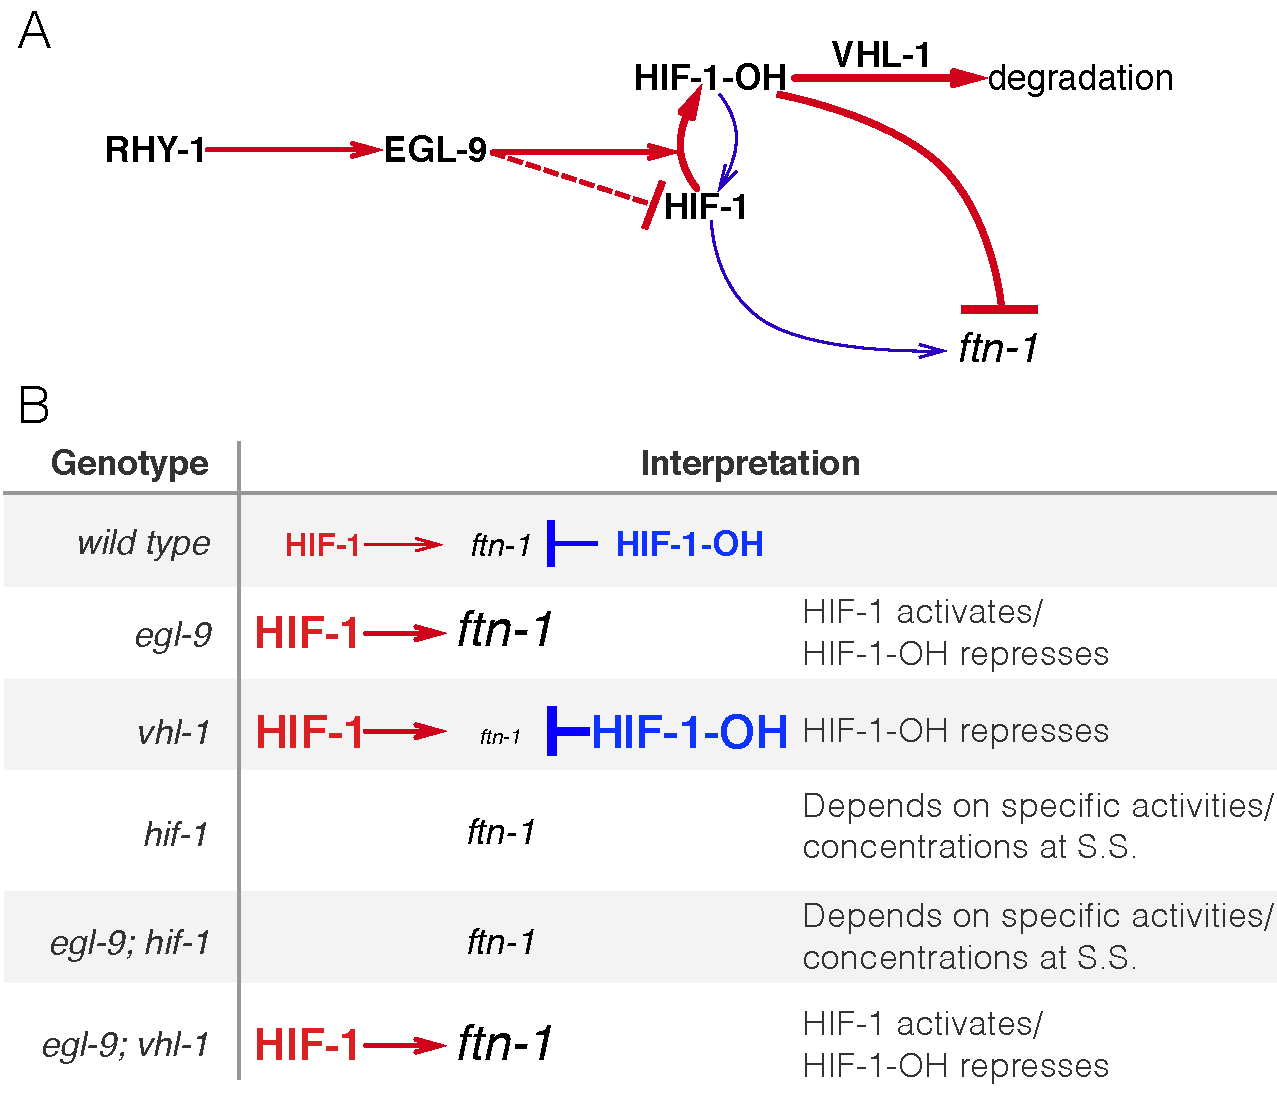
\includegraphics[width=.5\linewidth]{hypims/hif1oh_model.pdf}
\caption{
A hypothetical model showing a mechanism where \hifp{}-hydroxyl antagonises
\hifp{}.
\textbf{A}. Diagram showing that RHY-1 activates EGL-9.
EGL-9 hydroxylates HIF-1 in an oxygen dependent fashion. Under normoxia, HIF-1
is rapidly hydroxylated and only slowly does hydroxylated HIF-1 return to its
original state. EGL-9 can also inhibit HIF-1 in an oxygen-independent fashion.
HIF-1 hydroxyl is rapidly degraded in a VHL-1 dependent fashion. In our model,
HIF-1 and HIF-1 hydroxyl have opposing effects on transcription. The width of the
arrows represents the rates under normoxic conditions.
\textbf{B}. Table showing the effects of loss-of-function mutations on HIF-1 and
HIF-1 hydroxyl activity, showing how this can potentially explain the behavior
of \gene{ftn-1} in each case.  S.S = Steady-state.
}
\label{fig:hif1oh_table}
\end{figure}

One way to resolve this problem without invoking additional genes is to
consider \hifp{} as a protein with both activating and inhibiting states. In fact,
\hifp{} already exists in two states in \cel{}: unmodified \hifp{} and
\hifp{}-hydroxyl (\hifp{}-OH). Under this model, \hifp{}-hydroxyl antagonizes
the effects of \hifp{} for certain genes like \ftna{} or \nlp{}. Loss of
\gene{vhl-1} stabilizes \hifp{}-hydroxyl.
A subset of genes that are sensitive to \hifp{}-hydroxyl will be inhibited as a
result of the increase in the amount of this species, in spite of loss of
\gene{vhl-1} function also increasing the level of non-hydroxylated \hifp{}.
On the other hand, \egl{} selectively removes all \hifp{}-hydroxyl, stimulating
accumulation of \hifp{} and promoting gene activity. Whether deletion of \hif{}
is overall activating or inhibiting will depend on the relative activity of each
protein state under normoxia (see Fig.~\ref{fig:hif1oh_table}).

Multiple lines of circumstantial evidence that \hifp{}-hydroxyl plays a role
in the functionality of the hypoxia pathway. First, \hifp{}-hydroxyl is
challenging to study genetically because no mimetic mutations are available with
which to study the pure hydroxylated \hifp{} species. Second, although mutations in
the Von-Hippel Landau gene stabilize the hydroxyl species, they also increase the
quantity of non-hydroxylated \hifp{} by mass action.
Finally, since \hifp{} is detected low levels
in cells under normoxic conditions~\citep{Wang1993}, total \hifp{} protein
(unmodified \hifp{} plus \hifp{}-hydroxyl) is often tacitly assumed to be
vanishingly rare and therefore biologically inactive.

Our data show hundreds of genes that change expression in response
to loss of \gene{hif-1} under normoxic conditions. This establishes that there is
sufficient total \hifp{} protein to be biologically active.
Our analyses also revealed that \hif{} shares
positive correlations with \egl{}, \rhy{} and \vhl{}, and that each of these genotypes
also shows a secondary negative rank-ordered expression correlation with each other.
These cross-patterns between all loss of function of inhibitors of \hifp{} and
\hif{} can be most easily explained if \hifp{}-hydroxyl is biologically active.

A homeostatic argument can be made in favor of the activity of \hifp{}-hydroxyl.
At any point in time, the cell must measure the levels of
multiple metabolites at once. The \gene{hif-1}-dependent hypoxia
response integrates information from O$_2$, $\alpha$-ketoglutarate
(2-oxoglutarate) and iron concentrations in the cell. One way to
integrate this information is by encoding it only in the effective hydroxylation
rate of \hifp{} by \eglp{}. Then the dynamics in this system will evolve
exclusively as a result of the total amount of \hifp{} in the cell. Such a system
can be sensitive to fluctuations in the absolute concentration of
\hifp{}~\citep{Goentoro2009a}. Since the absolute levels of \hifp{} are low in
normoxic conditions, small fluctuations in protein copy-number represent can
represent a large fold-change in \hifp{} levels. These fluctuations would
not be problematic for genes that must be turned on only under conditions of severe
hypoxia---presumably, these genes would be associated with low affinity
sites for \hifp{}, so that they are only activated when \hifp{} levels are far
above random fluctuations.

For yet other sets of genes that must change expression in response to the hypoxia
pathway, it may not make as much sense to integrate metabolite information
exclusively via \eglp{}-dependent hydroxylation of \hifp{}. In particular, genes
that may function to increase survival in mild hypoxia may benefit from regulatory
mechanisms that can sense minor changes in environmental conditions and which
therefore benefit from robustness to transient changes in protein copy number.
Likewise, genes that are involved in iron or $\alpha$-ketoglutarate metabolism
(such as \ftna{}) may benefit from being able to sense, accurately, small and
consistent deviations from basal concentrations of these metabolites. For these
genes, the information may be better encoded by using \hifp{} and
\hifp{}-hydroxyl as an activator/repressor pair. Such circuits are
known to possess distinct advantages for controlling output in a manner that
is robust to transient fluctuations in the levels of their
components~\citep{Hart2012,Hart2013}.

Our RNA-seq data suggests that one of these atypical targets of \hifp{}
may be \rhyp{}. Although \gene{rhy-1} does not exhibit non-classical
epistasis, \hif{} and \eglhif{} both had increased expression levels of \gene{rhy-1}.
We speculate that if \gene{rhy-1} is controlled by both \hifp{} and \hifp{}-hydroxyl,
then this might imply that \hifp{} regulates the expression of its pathway (and
therefore itself) in a manner that is robust to total \hifp{} levels.

\subsection*{Insights into genetic interactions from vectorial phenotypes}

Here, we have described a set of straightforward methods that can be in theory
applied to any vectorial phenotype. Genome-wide methods afford a lot of information,
but genome-wide interpretation of the results is often extremely challenging.
Each method has its own advantages and disadvantages. We briefly discuss these
methods, their uses and their drawbacks.

Principal component analysis
is computationally tractable and clusters can often be visually detected with
ease. However, PCA can be misleading, especially when the dimensions represented
do not explain a very large fraction of the variance present in the data. In addition,
principal dimensions are the product of a linear combination of vectors, and therefore
must be interpreted with extreme care. In this case, the first principal dimension
separated genotypes that increase \hifp{} protein levels from those that decrease
it, but this dimension is a mix of vectors of change in gene expression. Although
PCA showed that there is information hidden in these genotypes, it was not enough
by itself to provide biological insight.

Whereas PCA operates on all genotypes simultaneously, correlation analysis is a
pairwise procedure that measures how predictable the gene
expression changes are in a mutant given the vector of expression changes in
another. Like PCA, correlation analysis is easy and fast to perform. Unlike PCA,
the product of a correlation analysis is a single number with a straightforward
interpretation. However, correlation analysis is particularly sensitive to outliers.
Although a common strategy is to rank-transform expression data to mitigate
outliers, rank-transformations do not remove the cross-patterns that appear when
feedback loops or other complex interactions are present between two genes.
Such cross-patterns can still lead to vanishing correlations if both patterns are
equally strong. Therefore, correlation analyses must take into account the possible
existence of systematic outliers. Moreover, correlation values must be measured
for both interactions in cross-patterned rank plots. Weighted correlations could
be informative for ordering genes along pathways.
A drawback of correlation
analysis is that the number of pairwise comparisons that must be made increases
combinatorially, though strategies could be used to decrease the total number of
effective comparisons.

Epistasis plots are a novel way to visualize epistasis in vectorial phenotypes.
Here, we have shown how an epistasis plot can be used to identify interactions
between two single mutants and a double mutant. In reality, epistasis plots
can be generated for any set of measurements involving a set of $N$ mutants and
an $N$-mutant genotype. Epistasis plots can accumulate an arbitrary number of
points within them, possess a rich structure that can be visualized and have
straightforward interpretations for special slope values.

Another way to analyze epistasis is via general linear models (GLMs) that include
interaction terms between two or more genes. In this way, GLMs can quantify
the epistatic effect of an interaction on single genes. We and
others~\citep{Dixit2016,Angeles-Albores2016a} have previously used GLMs to identify
gene sets that are epistatically regulated by two or more inputs. While powerful,
GLMs suffer from the multiple comparison problem. Correcting for false positives
using well-known multiple comparison corrections such as FDR~\citep{Storey2003}
tends to increase false negative rates.  Moreover, since GLMs attempt to estimate
effect magnitudes for individual gene or isoform expression levels, they
effectively treat each gene as an independent quantity, which prevents better
estimation of the magnitude and direction of the epistasis between two genes.

Epistasis plots do not suffer from the multiple comparison problem because the
number of tests performed is orders of magnitudes smaller than the number
of tests performed by GLMs. Ideally, in an epistasis plot we need only perform
3 tests---rejection of additive, unbranched and suppressive null models---compared
with the tens of thousands of tests that are performed in GLMs. Moreover, the
magnitude of epistasis between two genes can be estimated using hundreds of genes,
which greatly improves the statistical resolution of the epistatic coefficient.
This increased resolution is important because the size and magnitude of the
epistasis has specific consequences for the type of pathway that is expected.

Any quantitative use of genome-wide datasets requires a good experimental setup.
Here, we have demonstrated that whole-organism RNA-seq can be used to dissect
molecular pathways in exquisite detail when paired with experimental designs that
are motivated by classical genetics. Much more research will be necessary
to understand whether epistasis has different consequences in the microscopic
realm of transcriptional phenotypes than in the macroscopic world that geneticists
have explored previously. Our hope is that these tools, coupled with the classic
genetics experimental  designs, will reveal hitherto unknown aspects of genetics
theory.

\section*{Methods}
\label{sec:methods}
\subsection*{Nematode strains and culture}
Strains used were N2 wild-type Bristol,
CB5602 \gene{vhl-1}(\emph{ok161}),
CB6088 \gene{egl-9}(\emph{sa307})~\gene{hif-1}(\emph{ia4}),
CB6116 \gene{egl-9}(\emph{sa307});\gene{vhl-1}(\emph{ok161}),
JT307 \gene{egl-9}(\emph{sa307}),
ZG31 \gene{hif-1}(\emph{ia4}),
RB1297 \gene{rhy-1}(\emph{ok1402}).
All lines were grown on standard
nematode growth media (NGM) plates seeded with OP50 \ecol{} at 20\degree{}C
(Brenner 1974).

\subsection*{RNA Isolation}
Unsynchronized lines were grown on NGM plates at 20C and eggs harvested by
sodium hypochlorite treatment. Eggs were plated on 6 to 9 6cm NGM plates
with ample OP50 \ecol{} to avoid starvation and grown at
20\degree{}C.  Worms were staged and harvested based on the time after plating,
vulva morphology and the absence of eggs.  Approximately 30--50 non-gravid young
adults were picked and placed in 100$\mu$L of TE pH 8.0 at 4\degree{}C in
$0.2$mL PCR tubes.   After settling and a brief spin in microcentrifuge
approximately $80\mu$L of TE (Ambion AM 9849) was removed from the top of the
sample and individual replicates
were snap frozen in liquid N2. These replicate samples were then digested with
Proteinase K (Roche Lot No. 03115 838001 Recombinant Proteinase K PCR Grade) for
15min at 60\degree{} in the presence of 1\% SDS and 1.25$\mu$L
RNA Secure (Ambion AM 7005). RNA samples were then taken up in 5 Volumes of
Trizol (Tri Reagent Zymo Research) and processed and treated with DNase I using
Zymo MicroPrep RNA Kit (Zymo Research Quick-RNA MicroPrep R1050).
RNA was eluted in RNase-free water and divided into aliquots and stored at
-80\degree{}C. One aliquot of each replicate was analyzed using a NanoDrop (Thermo
Fisher) for impurities, Qubit for concentration and then analyzed on an Agilent
2100 BioAnalyzer (Agilent Technologies).
Replicates were selected that had RNA integrity numbers (RIN) equal or greater
than 9.0 and showed no evidence of bacterial ribosomal bands, except for the
ZG31 mutant where one of three replicates had a RIN of 8.3.

\subsection*{Library Preparation and Sequencing}
10ng of quality checked total RNA from each sample was
reverse-transcribed into cDNA using the Clontech SMARTer Ultra Low Input RNA for
Sequencing v3 kit (catalog \#634848) in the SMARTSeq2 protocol
~\citep{Picelli2014}.  RNA was denatured at 70$\degree{}$C for 3 minutes
in the presence of dNTPs, oligo dT primer and spiked-in quantitation standards
(NIST/ERCC from Ambion, catalog \#4456740).  After chilling to 4$\degree{}$C, the
first-strand reaction was assembled using the LNA TSO primer described in
\citet{Picelli2014}, and run at 42$\degree{}$C for 90 minutes, followed by
denaturation at 70$\degree{}$C for 10 minutes.  The entire first strand reaction
was then used as template for 13 cycles of PCR using the Clontech v3 kit.
Reactions were cleaned up with 1.8X volume of Ampure XP SPRI beads (catalog
\#A63880) according to the manufacturer’s protocol.  After quantification using
the Qubit High Sensitivity DNA assay, a 3ng aliquot of the amplified cDNA was
run on the Agilent HS DNA chip to confirm the length distribution of the
amplified fragments.  The median value for the average cDNA lengths from all
length distributions was 1076bp.  Tagmentation of the full length cDNA for
sequencing was performed using the Illumina/Nextera DNA library prep kit (catalog
\#FC-121--1030).  Following Qubit quantitation and Agilent BioAnalyzer profiling,
the tagmented libraries were sequenced. Libraries were sequenced on Illumina
HiSeq2500 in single read mode with the read length of 50nt to an average depth
of 15 million reads per sample following manufacturer's instructions. Base calls
were performed with RTA 1.13.48.0 followed by conversion to FASTQ with bcl2fastq
1.8.4. Spearman correlation of the transcripts per million (TPM) for each
genotype showed that every pairwise correlation within genotype was $>0.9$.

\subsection*{Read Alignment and Differential Expression Analysis}
We used Kallisto to perform read pseudo-alignment and performed differential
analysis using Sleuth. We fit a general linear model for a transcript $t$ in
sample $i$:

\begin{equation}
  y_{t,i} = \beta_{t, 0} + \beta_{t, genotype}\cdot{}X_{t, i} +
  \beta_{t, batch}\cdot{}Y_{t, i} + \epsilon_{t, i}
\end{equation}

where $y_{t, i}$ are the logarithm transformed counts; $\beta_{t, genotype}$ and
$\beta_{t, batch}$ are parameters of the model, and which can be interpreted as
biased estimators of the log-fold change; $X_{t, i}, Y_{t, i}$ are indicator
variables describing the conditions of the sample; and $\epsilon_{t, i}$ is the
noise associated with a particular measurement.

\subsection*{Genetic Analysis, Overview}
Genetic analysis of the processed data was performed in Python 3.5. Our scripts
made extensive use of the Pandas, Matplotlib, Scipy, Seaborn, Sklearn, Networkx,
Bokeh, PyMC3, and TEA libraries~\citep{Team2014,McKinney2011,Oliphant2007,
Pedregosa2012,Salvatier2015,VanDerWalt2011,Hunter2007,Angeles-Albores2016,Waskom}.
Our analysis is available in a Jupyter Notebook~\citep{Perez2007}. All code and
required data (except the raw reads) are available at
\url{https://github.com/WormLabCaltech/mprsq} along with version-control
information. Our Jupyter Notebook and interactive graphs for this project can be
found at \url{https://wormlabcaltech.github.io/mprsq/}. Raw reads were deposited
in the Short Read Archive under the study accession number SRP100886.


\subsection*{Weighted Correlations}
Pairwise correlations between transcriptomes where calculated by first identifying
the set of differentially expressed genes (DEGs) common to both transcriptomes under
analysis. DEGs were then rank-ordered according to their regression coefficient,
$\beta$.\ Bayesian robust regressions were performed using a Student-T distribution.
Bayesian analysis was performed using the PyMC3 library~\citep{Salvatier2015}
(\texttt{pm.glm.families.StudenT} in Python). If the correlation has an average
value $>1$, the correlation coefficient was set to 1.

Weights were calculated as the proportion of genes that were $<1.5$ standard
deviations away from the primary regression out of the entire set of shared DEGs
for each transcriptome.

\subsection*{Epistasis Analysis}
For a double mutant $X^-Y^-$, we used the single mutants $X^-$ and $Y^-$ to
find expected value of the coefficient for a double mutant under an additive model
for each isoform $i$.
Specifically,
\begin{equation}
  \beta_{\mathrm{Add},i} = \beta_{X,i} + \beta_{Y,i}.
\end{equation}

Next, we find the difference, $\Delta_i$, between the observed double mutant
expression coefficient, $\beta_{XY, \mathrm{Obs},i}$, and the predicted
expression coefficient under an additive model for each isoform $i$.

To calculate the transcriptome-wide epistasis coefficient, we plotted
($\beta_{\mathrm{Add},i}, \Delta_i$) and found the line of best fit using
orthogonal distance regression using the \texttt{scipy.odr} package in Python.
We performed
non-parametric bootstrap sampling of the ordered tuples with replacement using
5,000 iterations to generate a probability distribution of slopes of best fit.

There are as many models as epistatic relationships. For quantitative phenotypes,
epistatic relationships (except synthetic interactions) can be generally
expressed as:

\begin{equation}
  \beta_{XY} = \sum_{g\in G} \lambda_g \beta_g,
  \label{eq:epi}
\end{equation}

where $P_i$ is the quantitative phenotype belonging to the genotype $i$; $G$ is
the set of single mutants $\{X, Y\}$ that make up the double mutant, $XY$; and
$\lambda_g$ is the contribution of the phenotype $P_g$ to $P_{XY}$.
Additive interactions between genes are the result of setting $\lambda_g=1$. All
other relationships correspond to setting  $\lambda_X=0,~\lambda_Y=1$ or
$\lambda_X=1,~\lambda_Y=0$.

A given epistatic interaction can be simulated by predicting the double mutant
phenotype under that interaction and re-calculating the y-coordinates. The
recalculated y-coordinates can then be used to predict the possible epistasis
coefficients for the cases where $X$ is epistatic over $Y$, and $Y$ is epistatic
over $X$.

To select between theoretical models, we implemented an approximate Bayesian
Odds Ratio. We defined a free-fit model, $M_1$, that found the line of best fit
for the data:

\begin{equation}
  P(\alpha~|M_1, D) \propto \prod_{(x_i, y_i, \sigma_i)\in D}
  \exp{\frac{
            (y_i - \alpha\cdot x_i)^2
            } % numerator
            {
            2\sigma_i
            } % denominator
            } \cdot (1+\alpha^2)^{-3/2},
  \label{eq:free_model}
\end{equation}

where $\alpha$ is the slope of the model to be determined, $x_i, y_i$ were the
x- and y-coordinates of each point respectively, and $\sigma_i$ was the standard
error associated with the y-value. We minimized the
negative logarithm of equation~\ref{eq:free_model} to obtain the most likely
slope given the data, $D$ (\texttt{scipy.optimize.minimize} in Python). Finally,
we approximated the odds ratio as:

\begin{equation}
  OR = \frac{
  P(D~|\alpha^*, M_1)\cdot (2\pi)^{1/2}\sigma_{\alpha^*} % numerator
  }{P(D~| M_i)}, % denominator
\end{equation}

where $\alpha^*$ is the slope found after minimization, $\sigma_\alpha^*$ is the
standard deviation of the parameter at the point $\alpha^*$ and $P(D~|M_i)$ is the
probability of the data given the parameter-free model, $M_i$.

\subsection*{Enrichment Analysis}
Tissue, Phenotype and Gene Ontology Enrichment Analysis were carried out using
the WormBase Enrichment Suite for Python~\citep{Angeles-Albores2016b,
Angeles-Albores2016}.



\subsubsection*{Author Contributions:}
This work was supported by HHMI with whom PWS is an investigator
and by the Millard and Muriel Jacobs Genetics and Genomics Laboratory at
California Institute of Technology.
All strains were provided by the CGC, which is funded by NIH Office of Research
Infrastructure Programs (P40 OD010440).
This article was written with support of the Howard Hughes Medical Institute.
This article wouldn't be possible without help from Dr.\_ Igor Antoshechkin who
performed all sequencing.
We thank Hillel Schwartz for all of his careful advice.
We would like to thank Jonathan Liu, Han Wang, and Porfirio Quintero for helpful
discussion.

  % \printbibliography[heading=subbibliography]
\end{refsection}

\chapter{A study of dosage response in \cel{} using transcriptome profiling}
\begin{refsection}
  % \newcommand{\dicty}{\emph{D.~discoideum}}

% gene names
\newcommand{\nlp}{\emph{\mbox{nlp-31}}}
\newcommand{\ftna}{\emph{\mbox{ftn-1}}}
\newcommand{\ftnb}{\emph{\mbox{ftn-2}}}
\newcommand{\cysl}{\emph{\mbox{cysl-1}}}
\newcommand{\nog}{\emph{\mbox{nog-1}}}
\newcommand{\nhr}{\emph{\mbox{nhr-57}}}
\newcommand{\lam}{\emph{\mbox{lam-3}}}

\newcommand{\fog}{\emph{\mbox{fog-2(lf)}}}
\newcommand{\egl}{\emph{\mbox{egl-9}(lf)}}
\newcommand{\rhy}{\emph{\mbox{rhy-1}(lf)}}
\newcommand{\vhl}{\emph{\mbox{vhl-1}(lf)}}
\newcommand{\eglvhl}{\emph{\mbox{egl-9(lf);vhl-1(lf)}}}
\newcommand{\eglhif}{\emph{\mbox{egl-9(lf)}~\mbox{hif-1(lf)}}}
\newcommand{\hif}{\emph{\mbox{hif-1(lf)}}}

% protein names
\newcommand{\eglp}{EGL-9}
\newcommand{\rhyp}{RHY-1}
\newcommand{\nogp}{NOG-1}
\newcommand{\vhlp}{VHL-1}
\newcommand{\hifp}{HIF-1}
\newcommand{\fogp}{FOG-2}
\newcommand{\nhrp}{NHR-57}
\newcommand{\lamp}{LAM-3}
\newcommand{\cyslp}{CYSL-1}

% DE genes numbers:
\newcommand{\egln}{1,806}
\newcommand{\rhyn}{2,103}
\newcommand{\vhln}{689}
\newcommand{\eglvhln}{2,376}
\newcommand{\hifn}{546}
\newcommand{\eglhifn}{404}
\newcommand{\fogn}{2090}
\newcommand{\total}{5,671} % isoforms!!!!
% \newcommand{\inall}{53}
% \newcommand{\allup}{10}
% \newcommand{\alldown}{13}

% downstream targets
\newcommand{\egltargets}{126}
\newcommand{\rhytargets}{0}
\newcommand{\vhltargets}{45} % 44 genes, minus vhl-1 (IDed due to deletion)
\newcommand{\hiftargets}{195}
\newcommand{\hifohtargets}{31}


% website commands
\newcommand{\website}{
            \url{https://wormlabcaltech.github.io/Angeles_Leighton_2016/}
            }
\newcommand{\webref}{
\href{https://wormlabcaltech.github.io/Angeles_Leighton_2016/}{website}}

% more space between rows
\newcommand{\ra}[1]{\renewcommand{\arraystretch}{#1}}

\section*{Abstract}
\textbf{
RNA-seq is commonly used to identify genetic modules that respond to perturbations.
In single cells, transcriptomes have been used as phenotypes, but this concept
has not been applied to whole-organism RNA-seq. Linear models can quantify
expression effects of individual mutants and identify epistatic effects in double
mutants. However, interpreting these high-dimensional measurements is unintuitive.
We developed a single coefficient to quantify transcriptome-wide epistasis which
accurately reflects the underlying interactions. To demonstrate the power of our
approach, we sequenced four single and two double C. elegans mutants. From these
mutants, we successfully reconstructed the known hypoxia pathway. Using this
approach, we uncovered a class of 31 genes that have opposing changes in expression
in \egl{} and \vhl{} but the \eglvhl{} mutant phenocopies \egl{}.
These changes violate the classical model of HIF-1 regulation, but can be explained
by postulating a role of hydroxylated HIF-1 in transcriptional control.
}
\vspace{10mm}


\section*{Introduction}
\label{sec:introduction}
Genetic analysis of molecular pathways has traditionally been performed
through epistatis analysis. Generalized epistasis indicates that two genes interact
functionally; such interaction can involve the direct interaction of their
products or the interaction of any consequence of their function (small molecules,
physiological or behavioral effects)~\citep{Huang2006}. If two
genes interact, and the mutants of these genes have a quantifiable phenotype,
the double mutant of interacting genes will have a phenotype that is not the sum
of the phenotypes of the single mutants that make up its genotype. Epistasis
analysis remains a cornerstone of genetics today~\citep{Phillips2008}.


Recently, biological studies have shifted in focus from studying single
genes to studying all genes in parallel. In particular,
RNA-seq~\citep{Mortazavi2008} enables biologists to
identify genes that change expression in response to a perturbation. Gene expression
profiling using RNA-seq has become much more sensitive thanks to deeper and more
frequent sequencing due to lower sequencing costs~\citep{Metzker2010},
better and faster abundance quantification~\citep{Patro2014,Bray2016,Patro2015},
and improved differential expression analysis
methods~\citep{Pimentel2016,Trapnell2013}. RNA-seq has been
successfully used to identify genetic modules involved in a variety of processes,
including T-cell regulation~\citep{Singer2016,Shalek2013}, the
\emph{Caenorhabditis~elegans} (\cel{}) linker
cell migration~\citep{Schwarz2012}, and planarian stem cell
maintenance~\citep{VanWolfswinkel2014,Scimone2014}. For the most part, the role of
transcriptional profiling has been restricted to target gene identification.

Although transcriptional profiling has been primarily used for descriptive purposes,
transcriptomic phenotypes have previously been used to make genetic inferences.
Microarray analyses in \emph{S. cerevisiae} and \dicty{} were used to show
that transcriptomes can be interpreted to infer genetic relationships in simple
eukaryotes~\citep{Hughes2000, VanDriessche2005}.\@ eQTL studies in
many organisms, from yeast to humans, have established the usefulness of
transcriptomic phenotypes for population genetics studies~\citep{Brem2002,Schadt2003,
Li2006,King2014}. In cell culture, single-cell RNA-seq has seen significant
progress towards using transcriptomes as phenotypes with which to test genetic
interactions~\citep{Adamson2016,Dixit2016}.
More recently, we have identified a new developmental state
of \cel{} using whole-organism transcriptome profiling~\citep{Angeles-Albores2016a}.
To investigate the ability of whole-organism transcriptomes to serve as quantitative
phenotypes for epistasis analysis in metazoans, we sequenced the transcriptomes of
of four well-characterized loss of function mutants in the \cel{} hypoxia
pathway~\citep{Epstein2001,Shen2006,Shao2009,Jiang2001}.

% carmie:
Metazoans depend on the presence of oxygen in sufficient concentrations to
support aerobic metabolism. Genetic pathways evolved to rapidly respond to any
acute or chronic changes in oxygen levels at the cellular or organismal level.
Biochemical and genetic approaches identified the Hypoxia Inducible Factors
(HIFs) as an important group of oxygen-responsive genes that are involved in a
broad range of human pathologies~\citep{Semenza2012}.

Hypoxia Inducible Factors are highly conserved in metazoans~\citep{Loenarz2011}.
A common mechanism for hypoxia-response induction is heterodimerization between a
HIF$\alpha$ and a HIF$\beta$ subunit; the heterodimer then initiates
transcription of target genes~\citep{Jiang1996}. The number and complexity of
HIFs varies throughout metazoans, with humans having three HIF$\alpha$ subunits
and two HIF$\beta$ subunits, whereas in the roundworm \cel{} there is a single
HIF$\alpha$ gene, \gene{hif-1}~\citep{Jiang2001} and a single HIF$\beta$
gene, \gene{ahr-1}~\citep{Powell-Coffman1998}. HIF target genes have been implicated
in a wide variety of cellular and extracellular processes including glycolysis,
extracellular matrix modification, autophagy and immunity~\citep{Semenza1994,
Bishop2004,Shen2005,Bellier2009,Semenza2012}.

Levels of HIF$\alpha$ proteins tend to be tightly regulated. Under conditions of
normoxia, \hifp{}$\alpha$ exists in the cytoplasm and partakes in a futile cycle
of continuous protein production and rapid degradation~\citep{Huang1996}.
\hifp{}$\alpha$ is hydroxylated by three proline hydroxylases
in humans (PHD1, PHD2 and PHD3) but is only hydroxylated by one proline
hydroxylase (\eglp{}) in \cel{}~\citep{Kaelin2008}. \hifp{} hydroxylation
increases its binding affinity to Von Hippel Lindau Tumor Suppressor 1
(\vhlp{}), which allows ubiquitination of \hifp{} leading to its subsequent
degradation. In \cel{}, \eglp{} activity is inhibited by binding of \cyslp{},
and \cyslp{} activity is in turn inhibited at the protein level by \rhyp{},
possibly by post-translational modifications to \cyslp{}~\citep{Ma2012} (see
Fig.~\ref{fig:pathway}).

% heatmap
\begin{figure}[tbhp]
\centering
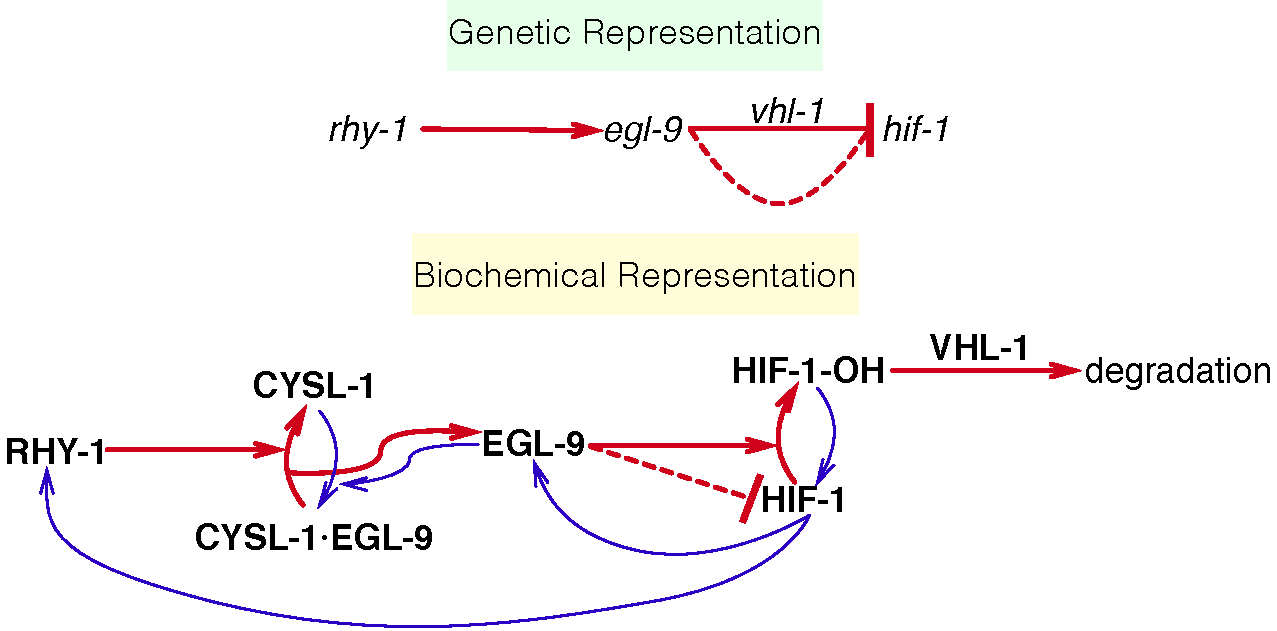
\includegraphics[width=.7\linewidth]{hypims/HIF1pathway.pdf}
\caption{
Genetic and biochemical representation of the hypoxia pathway in \cel{}.
Red arrows are arrows that lead to inhibition of \hifp{}, and blue arrows
are arrows that increase \hifp{} activity or are the result of \hifp{} activity.
\eglp{} is known to exert \gene{vhl-1}-dependent and independent repression
on \hifp{} as shown in the genetic diagram. The \gene{vhl-1}-independent
repression of \hifp{} by \eglp{} is denoted by a dashed line and is not dependent
on the hydroxylating activity of \eglp{}.
Technically, RHY-1 inhibits CYSL-1, which in turn inhibits EGL-9, but this
interaction was abbreviated in the genetic diagram for clarity.
}
\label{fig:pathway}
\end{figure}

Here, we show that transcriptomes contain robust signals that can be
used to infer relationships between genes in complex metazoans by reconstructing
the hypoxia pathway in \cel{} using RNA-seq.
Furthermore, we show that the phenomenon of phenotypic epistasis, a hallmark of
genetic interaction, holds at the molecular systems level.
We also demonstrate that transcriptomes contain sufficient information, under
certain circumstances, to order genes in a pathway using only single mutants.
Finally, we were able to identify genes that appear to be downstream of \gene{egl-9}
and \gene{vhl-1}, but do not appear to be targets of \gene{hif-1}.
Using a single set of genome-wide measurements, we were able to observe and
quantitatively assess  significant fraction of the known transcriptional
effects of \gene{hif-1} in \cel{}.
A complete version of the analysis, with ample documentation, is available at
\url{https://wormlabcaltech.github.io/mprsq}.

\section*{Results}
\subsection*{The hypoxia pathway controls thousands of genes in \cel{}}
\label{sub:summary}

We selected four single mutants within the hypoxia pathway for expression profiling:
\egl{} (\emph{sa307}), \rhy{} (\emph{ok1402}), \vhl{} (\emph{ok161}), \hif{} (\emph{ia4}).
We also sequenced the transcriptomes of two double mutants, \eglvhl{} (\emph{sa307},
\emph{ok161}) and \eglhif{} (\emph{sa307}, \emph{ia4}) as well as wild-type N2 as
a control sample. Each genotype  was sequenced in triplicate at a depth of 15
million reads. We performed whole-organism RNA-seq of these mutants at a moderate
sequencing depth ($\sim7$ million mapped reads for each individual replicate)
under normoxic conditions. For single samples, we identified around 22,000 different
isoforms per sample, which allowed us to measure differential expression of 18,344
isoforms across all replicates and genotypes (this constitutes  $\sim$70\% of
the protein coding isoforms in \cel{}).
We also included in our analysis a \fog{} (\emph{q71}) mutant which we have previously
studied~\citep{Angeles-Albores2016a}, because \gene{fog-2} is not reported to
interact with the hypoxia pathway.
We analyzed our data using a general linear model on
logarithm-transformed counts. Changes in gene expression are reflected in the
regression coefficient, $\beta$ which is specific to each isoform within a genotype.
Statistical significance is achieved when the q-values for each $\beta$ (p-values
adjusted for multiple testing) are less than 0.1. Genes that are significantly
altered between wild-type and a given mutant have $\beta$ values that are
statistically significantly different from 0.  These coefficients are not equal
to the average log-fold change per gene, although they are loosely related to
this quantity. Larger magnitudes of $\beta$ correspond to larger perturbations.
These coefficients can be used to study the RNA-seq data in question.

In spite of the moderate sequencing depth, transcriptome profiling of the hypoxia
pathway revealed that this pathway controls thousands of genes in \cel{}. The
\egl{} transcriptome showed differential expression of \egln{} genes. Similarly,
\rhyn{} genes were differentially expressed in \rhy{} mutants. The \vhl{}
transcriptome showed considerably fewer differentially expressed genes (\vhln{}),
possibly because it is a weaker controller of \hif{} than
\egl{}~\citep{Shao2009}. The \egl{};\vhl{} double mutant transcriptome showed
\eglvhln{} differentially expressed genes. The \hif{} mutant also showed a
transcriptomic phenotype involving \hifn{} genes. The \eglhif{} double mutant
showed a similar number of genes with altered expression (\eglhifn{} genes, see
Table~\ref{tab:genes}).

\begin{table}[tbhp]
  \centering
  \begin{tabular}{lr}
    \toprule{}
    Genotype & Differentially Expressed Genes \\
    \midrule{}
    \egl{} & \egln{}\\
    \rhy{} & \rhyn{}\\
    \vhl{} & \vhln{}\\
    \eglvhl{} & \eglvhln{}\\
    \eglhif{} & \eglhifn{}\\
    \fog{} & \fogn{}\\
    \bottomrule{}
  \end{tabular}
  \caption{Number of differentially expressed genes in each mutant.}
\label{tab:genes}
\end{table}

\subsection*{Principal Component Analysis visualizes epistatic relationships between genotypes}
\label{sub:Clustering}

Principal Component Analysis (PCA) is a well-known technique in bioinformatics that is
used to identify relationships between high dimensional data points~\citep{Yeung2001}
We performed PCA on our data to examine whether each genotype clustered in a biologically
relevant manner. PCA identifies the vector that can explain most of the variation
in the data;this is called the first PCA dimension. Using PCA, one can identify
the first $n$ dimensions that can explain more than 95\% of the variation in the
data. Sample clustering in these $n$ dimensions often indicates biological
relationships between the data, although interpreting PCA dimensions can be
difficult.

After applying PCA, we expected \hif{} to cluster near \eglhif{}, because
\hif{} exhibits no phenotypic defects under normoxic conditions, in contrast to
\egl{}, which exhibits an egg-laying (Egl) phenotype in the same environment.
In \eglhif{} mutants the Egl phenotype of \egl{} mutants is suppressed and instead
the grossly wild-type phenotype of \hif{} is observed. On the other hand, we
expected \egl{}, \rhy{}, \vhl{} and \eglvhl{} to form a separate cluster since
each of these genotypes is Egl and has a constitutive hypoxic response. Finally,
we included as a negative control a \fog{} mutant we have analyzed
previously~\citep{Angeles-Albores2016a}. This data was obtained at a different
time from the other genotypes, so we included a batch-normalization term in our
equations to account for this. Since \gene{fog-2} has not been described
to interact with the hypoxia pathway, we expected that it should appear far away
from either cluster.

The first dimension of the PCA analysis was able to discriminate between mutants
that have constitutive high levels of \hifp{} and mutants that have no \hifp{},
whereas the second dimension was able to discriminate between mutants within the
hypoxia pathway and outside the hypoxia pathway (see Fig.~\ref{fig:pca}).
Therefore expression profiling measures enough signal to cluster genes in a
meaningful manner in complex metazoans.

\begin{figure}[tbhp]
\centering
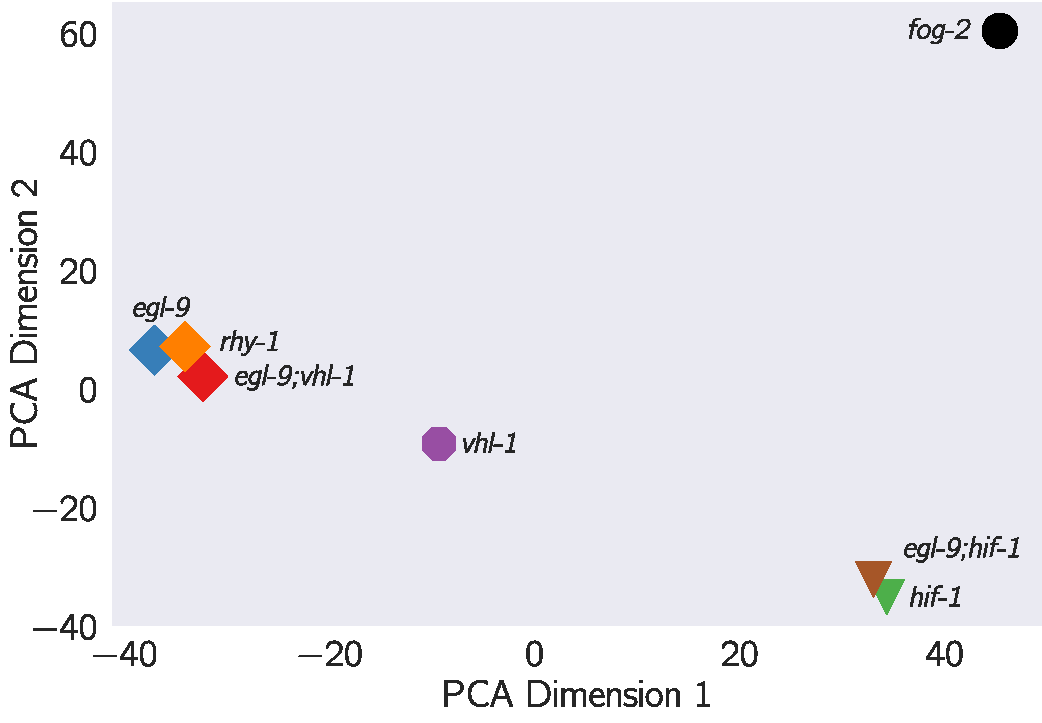
\includegraphics[width=0.5\linewidth]{hypims/pca.pdf}
\caption{
Principal component analysis of various \cel{} mutants. Genotypes that have an
activated hypoxia response (\emph{i.e}, \egl{}, \vhl{}, and \rhy{}) cluster far
from \hif{}. \hif{} clusters with the suppressed \eglhif{} double mutant.
The \fog{} transcriptome, used as an outgroup, is far away from either cluster.
}
\label{fig:pca}
\end{figure}

\subsection*{Reconstruction of the hypoxia pathway from first genetic principles}
\label{sec:reconstruct}
Having shown that the signal in the mutants we selected was sufficient to
cluster mutants using the values of the regression coefficients $\beta$, we set
out to reconstruct the hypoxia pathway from genetic first principles. In general,
to reconstruct a pathway, we must first assess whether two genes act on the same
phenotype. If they do not act on the same phenotype (the set of commonly differentially
regulated genes between two mutants is empty), these mutants are independent.
If they are not independent, then two mutants have a shared transcriptomic
phenotype (STP)---a set of genes or isoforms that are differentially expressed in
both mutants, without taking into account what direction they change in. In this
case, we must measure whether these genes act additively or epistatically on the
measured phenotype; if there is epistasis we must measure whether it is
positive or negative, in order to assess whether the epistatic relationship is a
genetic suppression or a synthetic interaction.

\subsubsection*{Genes in the hypoxia mutant act on the same transcriptional phenotype}
\label{sec:phenotypes}
We observed that all the hypoxia mutants had significant shared transcriptomic
phenotypes (fraction of the transcriptomes that was shared between mutants
ranged from a minimum of 6.8\% shared between \hif{} and \eglvhl{} to a maximum
of 31\% shared genes between \egl{} and \eglvhl{}). For comparison, we also
analyzed a previously published \fog{} transcriptome~\citep{Angeles-Albores2016a}.
The \gene{fog-2} gene is involved in masculinization of the \cel{} germline,
which enables sperm formation, and is not known to be involved in the hypoxia
pathway. The hypoxia pathway mutants and the \fog{} mutant also showed shared
transcriptomic phenotypes (3.6\%--12\% genes), but correlations between
expression level changes were considerably weaker (see below), suggesting that
there is minor cross-talk between these pathways.


% genetic correlations
\begin{figure}[tbhp]
\centering
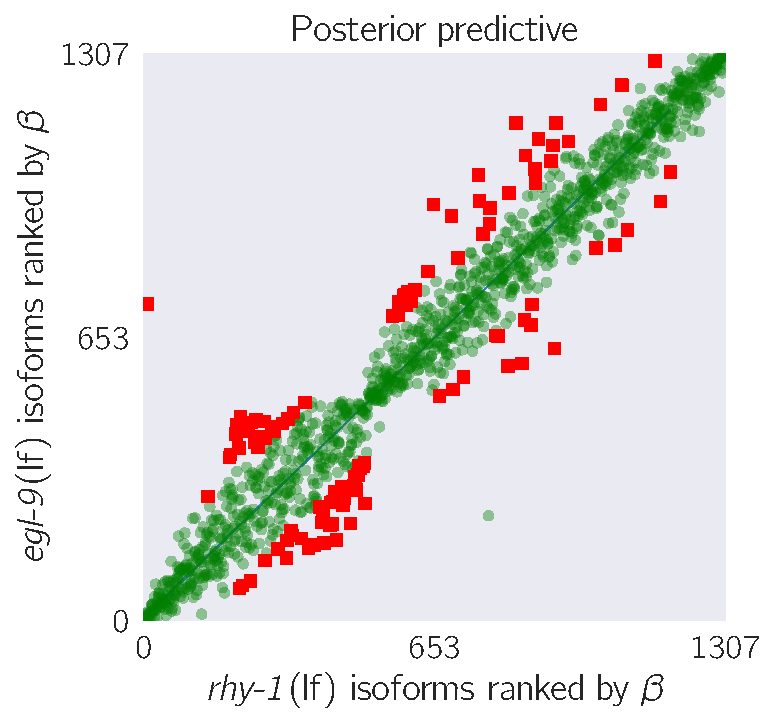
\includegraphics[width=.4\linewidth]{hypims/multiplemodes-eb.pdf}
\caption{
Strong transcriptional correlations can be identified between genes
that share a positive regulatory connection. We took the \egl{} and the \rhy{}
transcriptomes, identified differentially expressed genes common to both
transcriptomes and ranked each gene according to its differential expression
coefficient $\beta$. We plotted the rank of each gene in \rhy{} versus the
rank of the same gene in the \egl{} transcriptome. The result is an almost
perfect correlation. Green, transparent large points mark inliers to the primary
regressions (blue lines); red squares mark outliers to the primary regressions.
}
\label{fig:genetic_interactions}
\end{figure}

We wanted to know whether it was informative to look at quantitative agreement
within STPs. For each mutant pair, we rank-transformed
the regression coefficients $\beta$ of each isoform within the STP, and
calculated lines of best fit using Bayesian regression with a Student-T
distribution to mitigate noise from outliers and plotted the results in a rank plot
(see Fig~\ref{fig:genetic_interactions}). For transcriptomes associated with the
hypoxia pathway, we found that these correlations tended to have
values higher than 0.9 with a tight distribution around the line of best fit.
The correlations for mutants from the hypoxia pathway
with the \fog{} mutant were considerably weaker, with magnitudes between
0.6--0.85 and greater variance around the line of best fit.
Although \gene{hif-1} is known to be genetically repressed by \gene{egl-9}, \gene{rhy-1} and
\gene{vhl-1}~\citep{Epstein2001,Shen2006}, all the correlations
between mutants of these genes and \hif{} were positive.

After we calculated the pairwise correlation within each STP,
we weighted the result of each regression by the
number of isoforms within the STP and
divided by the total number of differentially expressed isoforms present in the
two mutant transcriptomes that contributed to that specific STP,
$N_\mathrm{overlap}/N_{\mathrm{g_1} \cup \mathrm{g2}}$.
The weighted regressions recapitulated a module network (see Fig.~\ref{fig:heatmap}).
We identified a strong positive interaction between \egl{} and \rhy{}.
The magnitude of this weighted correlation derives from the magnitude of the
transcriptomes for these mutants (\egln{} and \rhyn{} differentially expressed
genes respectively) and the overlap between both genes was
extensive, which makes the weighting factor considerably larger than other pairs.
The weak correlation between \hif{} and \egl{} results from the small size of
the \hif{} transcriptome and the small overlap between the transcriptomes.

The fine-grained nature of transcriptional phenotypes means that these weighted
correlations between transcriptomes of single mutants are predictive of genetic
interaction.

% heatmap
\begin{figure}[tbhp]
\centering
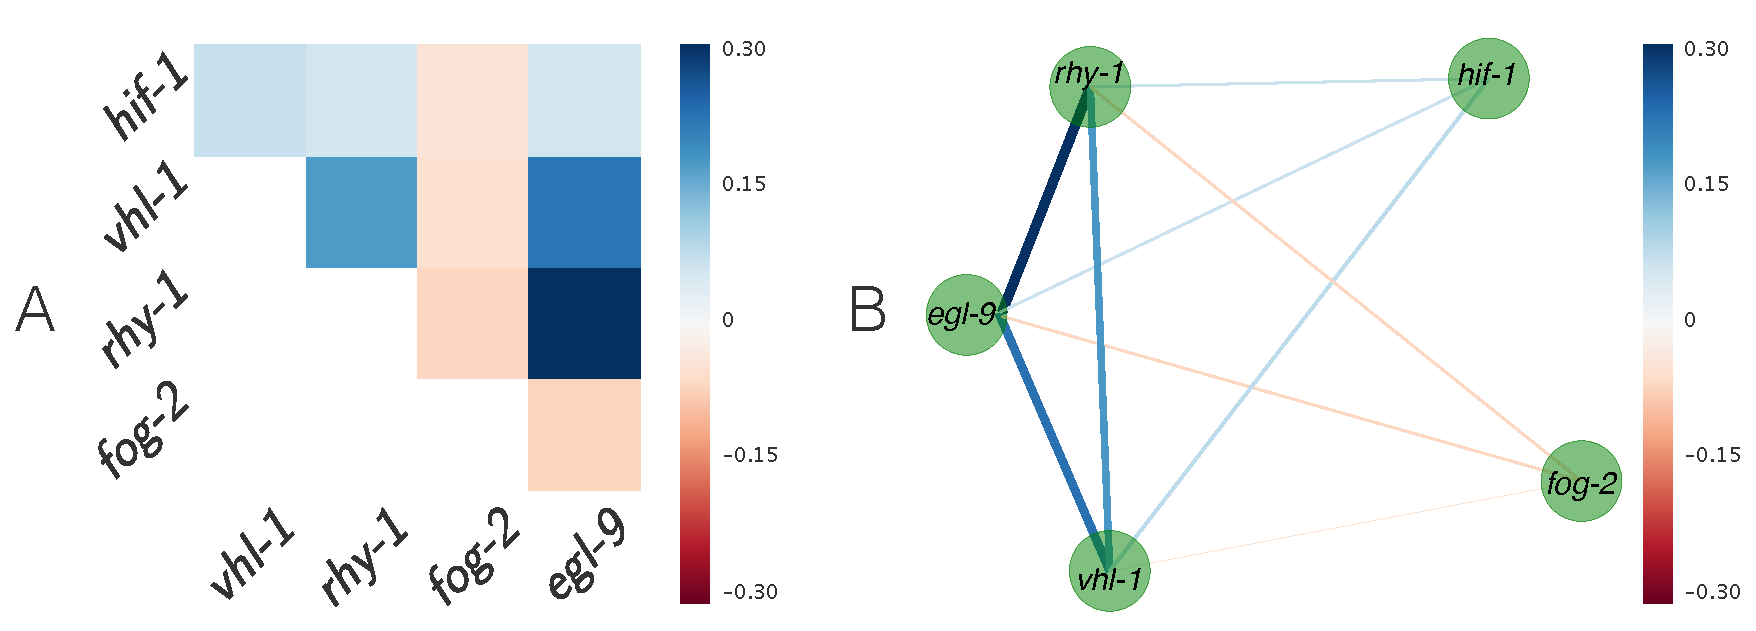
\includegraphics[width=\linewidth]{hypims/bayesian-heatmap-horizontal.pdf}
\caption{
\textbf{A}. Heatmap showing pairwise regression values between all
single mutants. \textbf{B}. Correlation network drawn from \textbf{A}. Edge
width is proportional to the logarithm of the magnitude of the weighted
correlation between two nodes divided by absolute value of the weighted
correlation value of smallest magnitude. Edges are also colored according to the
heatmap in \textbf{A}. Inhibitors of \gene{hif-1} are tightly correlated and form
a control module;
\gene{hif-1} is positively correlated to its inhibitors, albeit weakly;
and
\gene{fog-2}, a gene that is not reported to interact with the hypoxia pathway,
has the smallest, negative correlation to any gene.
}
\label{fig:heatmap}
\end{figure}

\subsubsection*{A quality check of the transcriptomic data reveals excellent agreement
            with the literature}
\label{sub:quality_check}
One way to establish whether genes are acting additively or epistatically to each
other is to perform qPCR of a reporter gene in the single and double mutants. This
approach was used to successfully map the relationships within the hypoxia
pathway (see, for example~\citep{Shao2009,Shen2006}). A commonly used hypoxia reporter
gene is \nhr{}, which is known to exhibit a several-fold increase in mRNA
expression when \hifp{} accumulates~\citep{Shen2006,Shen2005,Park2012}. Likewise,
increased \hifp{} fucntion is known to cause increased of \gene{rhy-1}
and \gene{egl-9}~\citep{Powell-Coffman2010}.

We can
selectively look at the expression of a few genes at a time. Therefore, we
queried the changes in expression of \gene{rhy-1}, \gene{egl-9}, and \nhr{}. We
included the nuclear laminin gene \lam{} as a representative negative control not
believed to be responsive to alterations in the hypoxia pathway.
\nhr{} was upregulated in \egl{}, \rhy{} and \vhl{}, but remains unchanged in \hif{}.
\eglvhl{} had an expression level similar to \egl{}; whereas the
\eglhif{} mutant showed wild-type levels of the reporter expression, as reported
previously~\citep{Shen2006} (see Fig.~\ref{fig:qpcr}).

% in silico qPCR
\begin{figure}[tbhp]
\centering
\includegraphics[width=.5\linewidth]{hypims/qpcr.pdf}
\caption{
\textbf{Top}: Observed $\beta$ values of select genes. We selected
four genes (\gene{rhy-1}, \gene{egl-9}, \nhr{} and \lam{}, shown on the x-axis)
and plotted their regression coefficients, $\beta$, as measured for every
genotype (represented by one of six colors) to study the epistatic relationships
between each gene. Asterisks above a bar represent a regression coefficient
statistically significantly different from 0 (\qval{1}) relative to a wild-type
control. Error bars show standard error of the mean
value of $\beta$. \nhr{} is an expression reporter that has been used previously
to identify \gene{hif-1} regulators~\citep{Shen2006,Shao2009}. \lam{} is shown here
as a negative control that should not be altered by mutations in this pathway.
We measured modest increases in the levels of \gene{rhy-1} mRNA when \hif{} is
knocked out.
}
\label{fig:qpcr}
\end{figure}

We observed changes in \rhy{} expression consistent with previous
literature~\citep{Shen2006} when \hifp{} accumulates.
We also observed increases in \gene{egl-9} expression in \egl{}.
\gene{egl-9} is known as a hypoxia responsive gene~\citep{Powell-Coffman2010}.
Although changes in \gene{egl-9} expression were not statistically significantly
different from the wild-type in
\rhy{} and \vhl{} mutants, the mRNA levels of \gene{egl-9} still trended towards
increased expression in these genotypes.
As with \nhr{}, \gene{egl-9} and \gene{rhy-1} expression were wild-type in
\eglhif{} and \eglvhl{} mutant showed expression phenotypes identical to \egl{}.
This dataset also showed that knockout of \gene{hif-1} resulted in a modest
increase in the levels of \gene{rhy-1}. This suggests that \gene{hif-1}, in
addition to being a positive regulator of \gene{rhy-1}, also inhibits it, which
constitutes a novel observation.
Using a single reporter we would have been able to reconstruct an
important fraction of the genetic relationships between the genes in the hypoxia
pathway–--but would likely fail to observe yet other genetic interactions, such as
the evidence for \gene{hif-1} negatively regulating \gene{rhy-1} transcript levels.


\subsection*{Transcriptome-wide epistasis}
Ideally, any measurement of transcriptome-wide epistasis should conform to certain
expectations. First, it should make use of the regression coefficients of as
many genes as possible. Second, it should be summarizable in a single,
well-defined number. Third, it should have an intuitive behavior, such that
special values of the statistic should each have an unambiguous interpretation.

One way of displaying transcriptome-wide epistasis is to plot transcriptome data onto
an epistasis plot (see Fig~\ref{fig:egl9epistasis}). In an epistasis plot, the
X-axis represents the expected expression of a double mutant $a^-b^-$ if $a$
and $b$ interact additively.
In other words, each individual isoform's x-coordinate is the sum of the regression
coefficients from the single mutants $a^-$ and $b^-$.
The Y-axis represents the deviations from the additive (null) model, and
can be calculated as the difference between the observed regression coefficient
and the predicted regression coefficient. Only genes that are differentially
expressed in all three genotypes are plotted. Assuming that the two genes interact
via a simple phenotype (for example, if both genes affect a transcription factor
that generates the entire transcriptome), these plots will generate specific
patterns that can be described through linear regressions. The slope of these
lines, $s_{a,b}$, is the transcriptome-wide epistasis coefficient.

Epistasis plots can be understood intuitively for simple cases of genetic
interactions. If two genes act additively on the same set of differentially expressed
isoforms then all the plotted points will fall along the line $y=0$.
If two genes interact in an unbranched pathway, then $a^-$ and $b^-$ should
have identical phenotypes for $a^-$, $b^-$ and $a^-b^-$, if all the genotypes are
homozygous for genetic null alleles~\citep{Huang2006}. It follows that the
data points should fall along a line with slope equal to $-\frac{1}{2}$. On the
other hand, in the limit of complete inhibition of $a$ by $b$, the plots should show
a line of best fit with slope equal to $-1$\footnote{Specifically, this follows
from assuming that $b^-$ is wild-type under the conditions assayed; and
$a^-b^-$ = $b^-$ = wild-type}.
Genes that interact synthetically (\emph{i.e.}, through an OR-gate) will fall
along lines with slopes $>0$. When there is epistasis of one gene over another,
the points will fall along a line of best fit with slope $s_{ab=b}$ or $s_{ab=a}$.
This slope must be determined from the single-mutant data.
From this information, we can use the single mutant data to predict the
distribution of slopes that results for each case stated above, as well as for
each epistatic combination ($a^-b^-=a^-$ or $a^-b^-=b^-$). The transcriptome-wide
epistasis coefficient ($s_{a, b}$), emerges as a powerful way to quantify epistasis
because it integrates information from many different genes or isoforms into a
single number (see Fig.~\ref{fig:egl9epistasis}).

In our experiment, we studied two double mutants, \eglhif{} and \eglvhl{}.
We wanted to understand how well an epistasis analysis based on transcriptome-wide
coefficients agreed with the epistasis results reported in the literature, which
were based on qPCR of single genes. Therefore, we performed orthogonal distance
regression on the two gene combinations we studied (\gene{egl-9} and
\gene{vhl-1}; and \gene{egl-9} and \gene{hif-1}) to determine the epistasis
coefficient for each gene pair. We also generated models for the special cases
mentioned above (additivity, $a^-b^-=a^-$, strong suppression, etc\ldots) using
the single mutant data. For every simulation, as well as for the observed data,
we used bootstraps to generate probability distributions of the epistasis
coefficients.

When we compared the predictions for the transcriptome-wide epistasis coefficient,
$s_{egl-9,vhl-1}$ under different assumptions with the observed slope ($-0.42$). We
observed that the predicted slope matched the simulated slope for the case where
\gene{egl-9} is epistatic over \gene{vhl-1} (\egl{} = \eglvhl{}, see
Fig.~\ref{fig:egl9epistasis}) and did not overlap with any other prediction.
Next, we predicted the distribution of $s_{egl-9,hif-1}$ for different pathways
and contrasted with the observed slope. In this case, we saw that the uncertainty
in the observed coefficient overlapped significantly with the strong suppression
model, where \eglp{} strongly suppresses \hifp{}, and also with the model where
\hif{} = \eglhif{}. In this case, both models are reasonable---\hifp{} is strongly
suppressed by \eglp{}, and we know from previous literature that the epistatic
relationship, \hif{} = \eglhif{}, is true for these mutants. In fact, as the
repression of \hifp{} by \eglp{} becomes stronger, the epistatic model should converge
on the limit of strong repression (see
\href{https://wormlabcaltech.github.io/mprsq/analysis_notebooks/epistasis_6.html}
{Epistasis}).

Another way to test which model best explains the epistatic relationship between
\gene{egl-9} and \gene{vhl-1} is to use Bayesian model selection to calculate
an odds ratio between two models to explain the observed data. Models can be placed
into two categories: parameter-free and fit. Parameter free models are `simpler'
because their parameter space is smaller (0 parameters) than the fit models ($n$
parameters). By Occam's razor, simpler models should be preferred to more
complicated models. However, simple models suffer from the drawback that
systematic deviations from them cannot be explained or accomodated, whereas more
complicated models can alter the fit values to maximize their explanatory power.
In this sense, more complicated models should be preferred when the data shows
systematic deviations from the simple model. Odds-ratio selection gives us a way
to quantify the trade-off between simplicity and explanatory power.

We reasoned that comparing a fit model ($y = \alpha\cdot x$, where $\alpha$ is
the slope of best fit) against a parameter-free model ($y = \gamma\cdot x$,
where $\gamma$ is a single number) constituted a conservative approach towards
selecting which theoretical model (if any) best explained the data. In particular,
this approach will tend to strongly favor the line of best fit over simpler model
for all but very small, non-systematic deviations. We decided
that we would reject the theoretical models only if the line of best-fit
was $10^3$ times more likely than the theoretical models (odds ratio, OR $>10^3$).
Comparing the odds-ratio between the line of best fit and the different pathway
models for \gene{egl-9} and \gene{vhl-1} showed similar results to the simulation.
Only the theoretical model \egl{} = \eglvhl{} could not be rejected (OR = 0.46),
whereas all other models were significantly less likely than the line of best fit
(OR $>10^{44}$).
Therefore, \gene{egl-9} is epistatic to \gene{vhl-1}. Moreover,
since $s_{egl-9, vhl-1}$ is strictly between and not equal to $0$ and $-0.5$, we
conclude that \gene{egl-9} acts on its transcriptomic phenotype in
\gene{vhl-1}-dependent and independent manners. A branched pathway that can lead
to epistasis coefficients in this range is a pathway where \gene{egl-9} interacts
with its transcriptomic phenotype via branches that have the same valence (both
positive or both negative)~\citep{Shao2009}. When we performed a similar analysis
to establish the epistatic relationship between \gene{egl-9} and \gene{hif-1},
we observed that the best alternative to a free-fit model was a model where
\gene{hif-1} is epistatic over \gene{egl-9} (OR$=2551$), but the free-fit model
was still preferred. All other models were strongly rejected (OR $>10^{25}$).

% epistasis graph
\begin{figure}[tbhp]
\centering
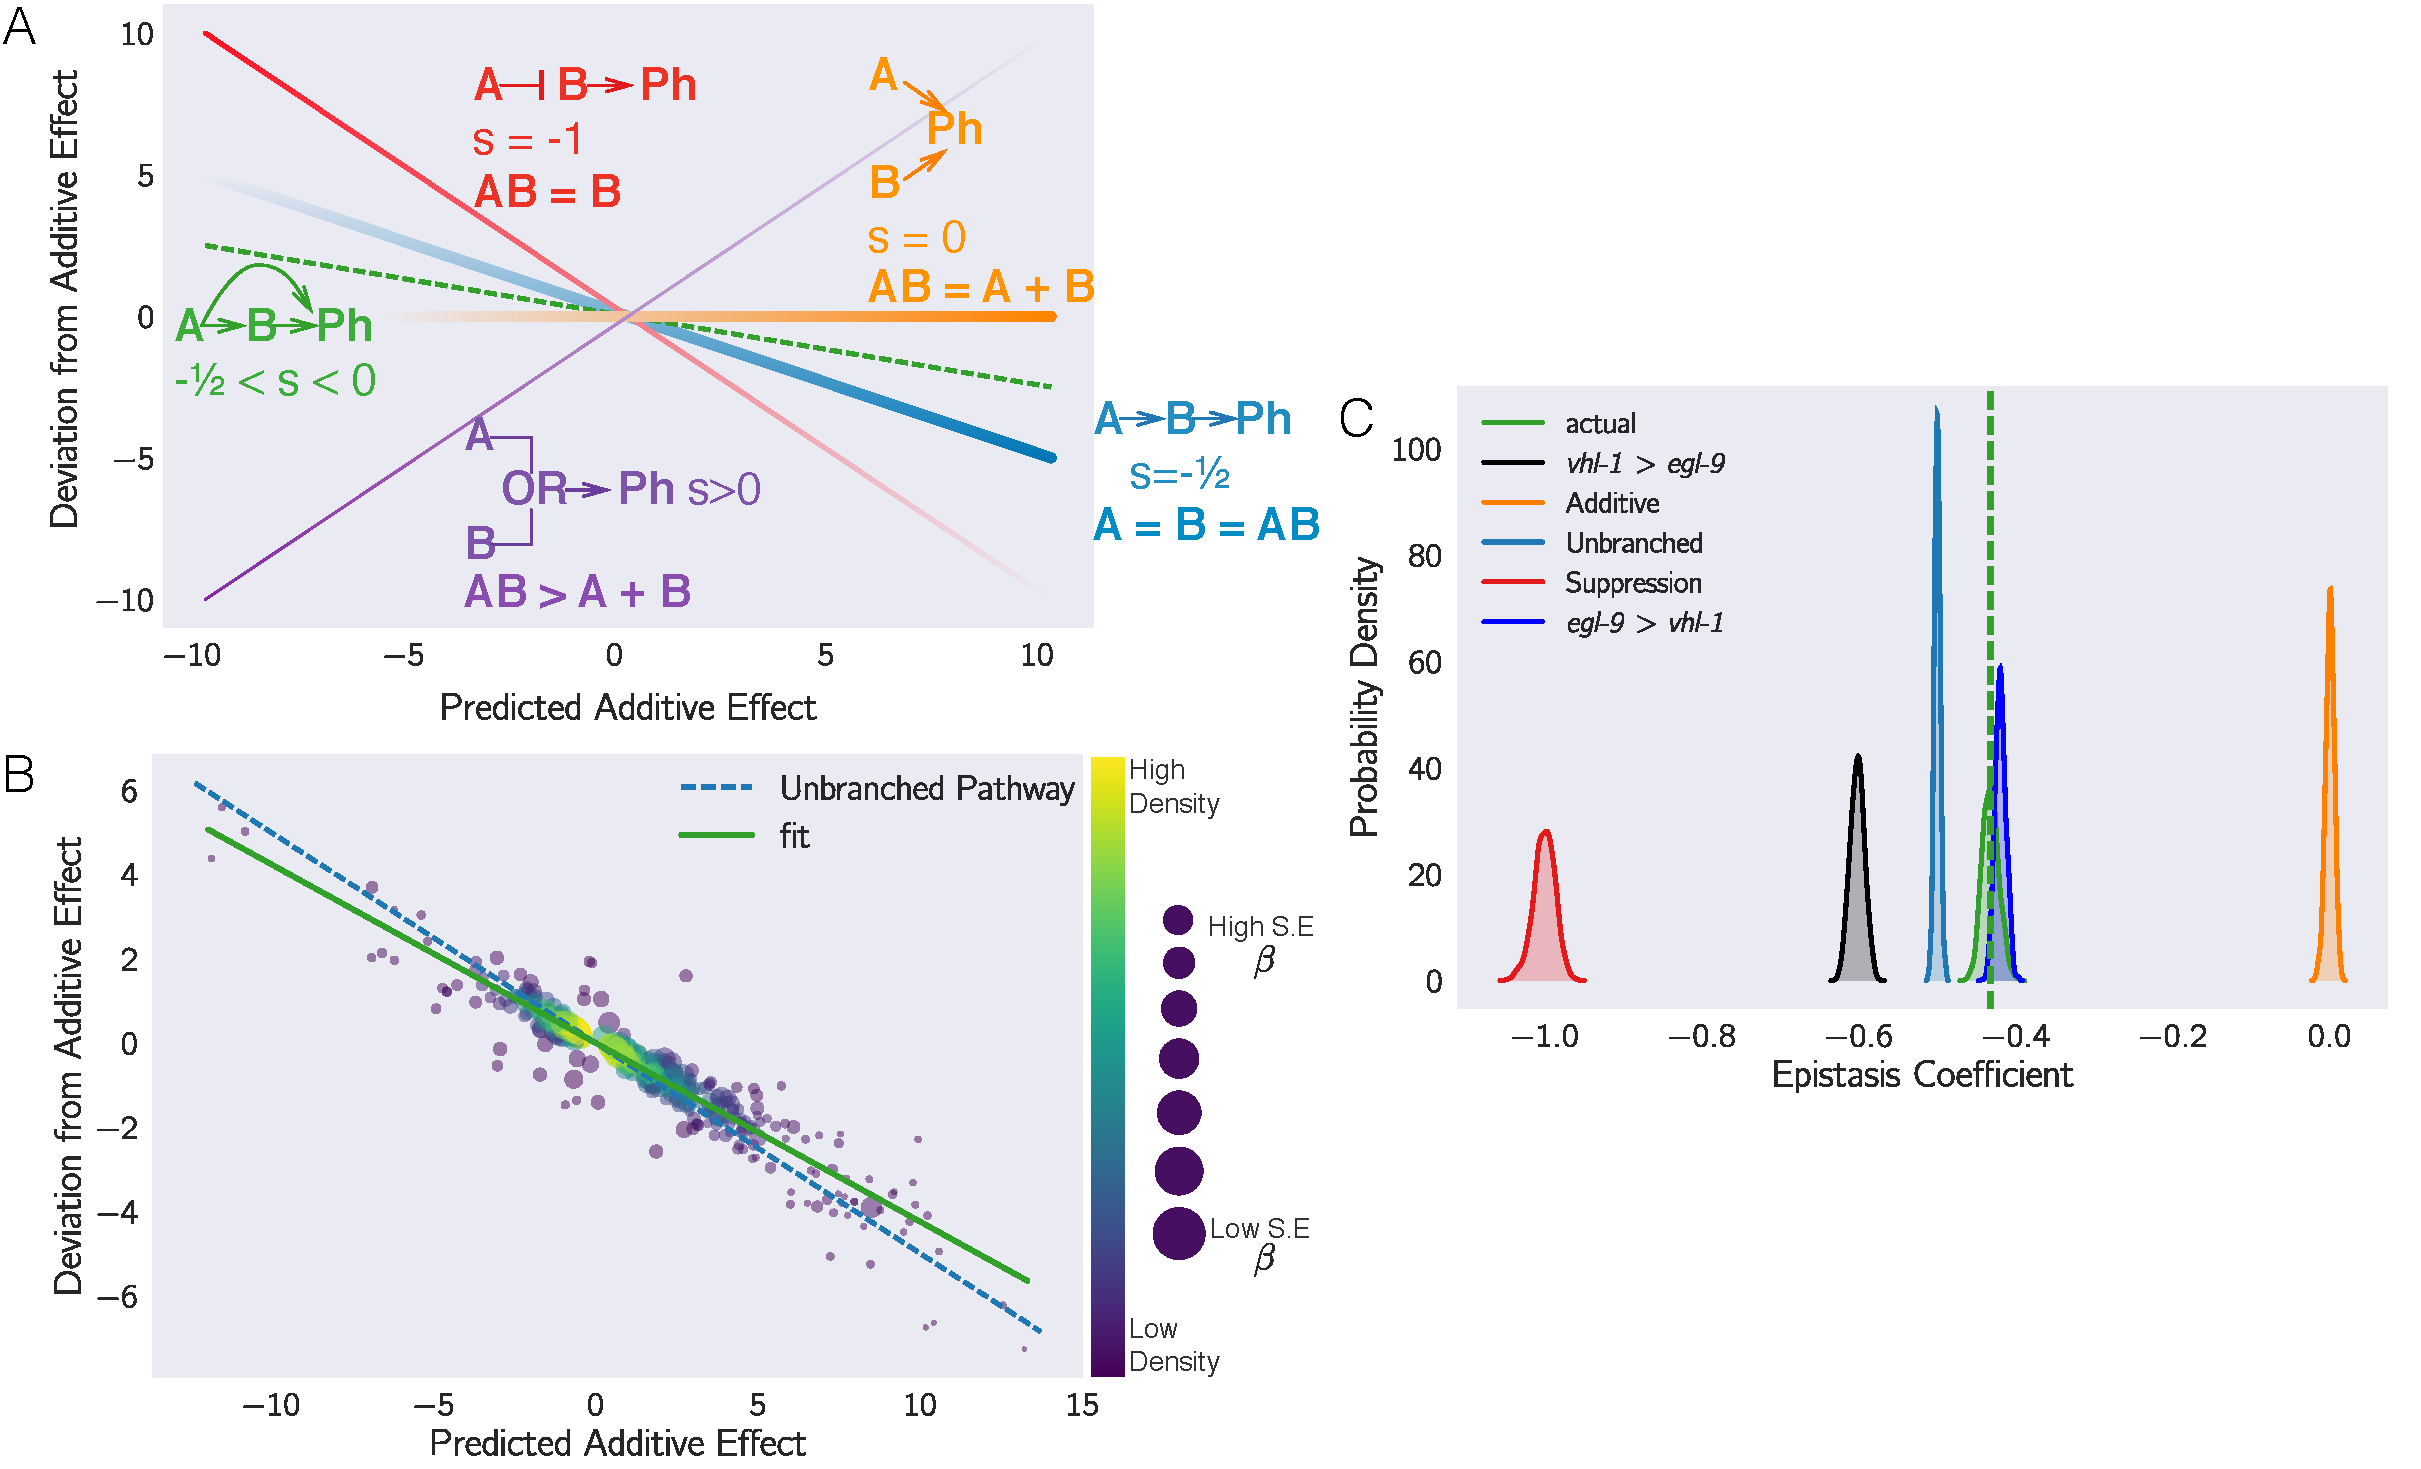
\includegraphics[width=\linewidth]{hypims/egl9hif1-epistasis-horizontal.pdf}
\caption{
(\textbf{A}) Schematic diagram of an epistasis plot. The X-axis on an epistasis
plot is the expected coefficient for a double mutant under an additive model
(null model). The Y-axis plots deviations from this model. Double mutants that
deviate in a systematic manner from the null model exhibit transcriptome-wide epistasis
($s$). To measure $s$, we perform a linear regression on the data. The slope of
the line of best fit is $s$. This coefficient is related to genetic architectures.
Genes that act additively on a phenotype \textbf{(Ph)} will have $s=0$ (orange
line); whereas
genes that act along an unbranched pathway will have $s=-1/2$ (blue line).
Strong
repression is reflected by $s=-1$ (red line). Cases where $s>0$ correspond to
synthetic interactions (purple line), and in the limit as $s\rightarrow\infty$,
the synthetic interaction
must be an OR-gate. Cases where $0 < s < -1/2$ correspond to circuits
that have multiple positive branches; whereas cases where
$-1/2<s< -1$ correspond to cases where the branches have different valence.
Cases where $s < -1$ represent inhibitory branches.
(\textbf{B}) Epistasis plot showing
that the \eglvhl{} transcriptome deviates significantly from a null additive.
Points are colored qualitatively according to density (purple---low,
yellow---high) and size is inversely proportional to the standard
error (S.E.) of the y-axis (larger points, higher accuracy). The purple line
is the line of best fit from an orthogonal distance regression.
(\textbf{C}) Comparison of simulated epistatic coefficients against the observed
coefficient. Green curve shows the bootstrapped observed transcriptome-wide epistasis
coefficient for \gene{egl-9} and \gene{vhl-1}. Dashed green line shows the mean
value of the data. Using the single mutants, we simulated coefficient
distributions for a linear model (light blue, centered at $-0.5$);
an additive model (orange, centered at 0); a model where either
\gene{egl-9} or \gene{vhl-1} masks the other phenotype (dark blue and black,
respectively) and a complete suppression model (red, centered at $-1$).
The observed coefficient overlaps the predicted epistasis curve for
\eglvhl{} = \egl{} (green and dark blue).
}
\label{fig:egl9epistasis}
\end{figure}

\subsubsection*{Epistasis can be predicted}
Given our success in measuring epistasis coefficients, we wanted to know whether
we could predict the epistasis coefficient between \gene{egl-9} and \gene{vhl-1}
in the absence of the \egl{} genotype. Since \rhyp{} indirectly activates
\eglp{}, the \rhy{} transcriptome should contain more or less
equivalent information to the \egl{} transcriptome. Therefore, we generated
predictions of the epistasis coefficient between \gene{egl-9} and \gene{vhl-1}
by substituting in the \rhy{} data. We predicted $s_{rhy-1,vhl-1} = -0.45$.
Similarly, we used the \eglvhl{} double mutant to
measure the epistasis coefficient while replacing the \egl{} dataset with the \rhy{}
dataset. We found that the epistasis coefficient using this substitution was $-0.40$.
This coefficient was different from $-0.50$ (OR $>10^{62}$), reflecting the same
qualitative conclusion that the hypoxia pathway is branched.
In conclusion, we were able to obtain a quantitatively close prediction of the
epistasis coefficient for two mutants using the transcriptome of a related,
upstream mutant. Finally, we showed that in the absence of a single mutant, an
upstream locus can under some circumstances be used to estimate epistasis
between two genes.


\subsection*{Transcriptomic decorrelation can be used to infer functional distance}
\label{sub:decorrelation}
% What are functional interactions?
So far, we have shown that RNA-seq can accurately measure genetic interactions.
However, genetic interactions are far removed from biochemical interactions:
Genetic interactions do not require two gene products to interact physically, nor
even to be physically close to each other. RNA-seq cannot measure physical
interactions between genes, but we wondered whether expression profiling contains
sufficient information to order genes along a pathway.

Single
genes are often regulated by multiple independent sources. The connection between
two nodes can in theory be characterized by the strength of the edges connecting
them (the thickness of the edge); the sources that regulate both
nodes (the fraction of inputs common to both nodes); and the genes that are
regulated by both nodes (the fraction of outputs that are common to both nodes).
In other words, we expected that expression profiles associated with a pathway
would respond quantitatively to quantitative changes in activity of the pathway.
Targeting a pathway at multiple points would lead to expression profile
divergence as we compare nodes that are separated by more degrees of freedom,
reflecting the flux in information between them.

% decorrelation
\begin{figure}[tbhp]
\centering
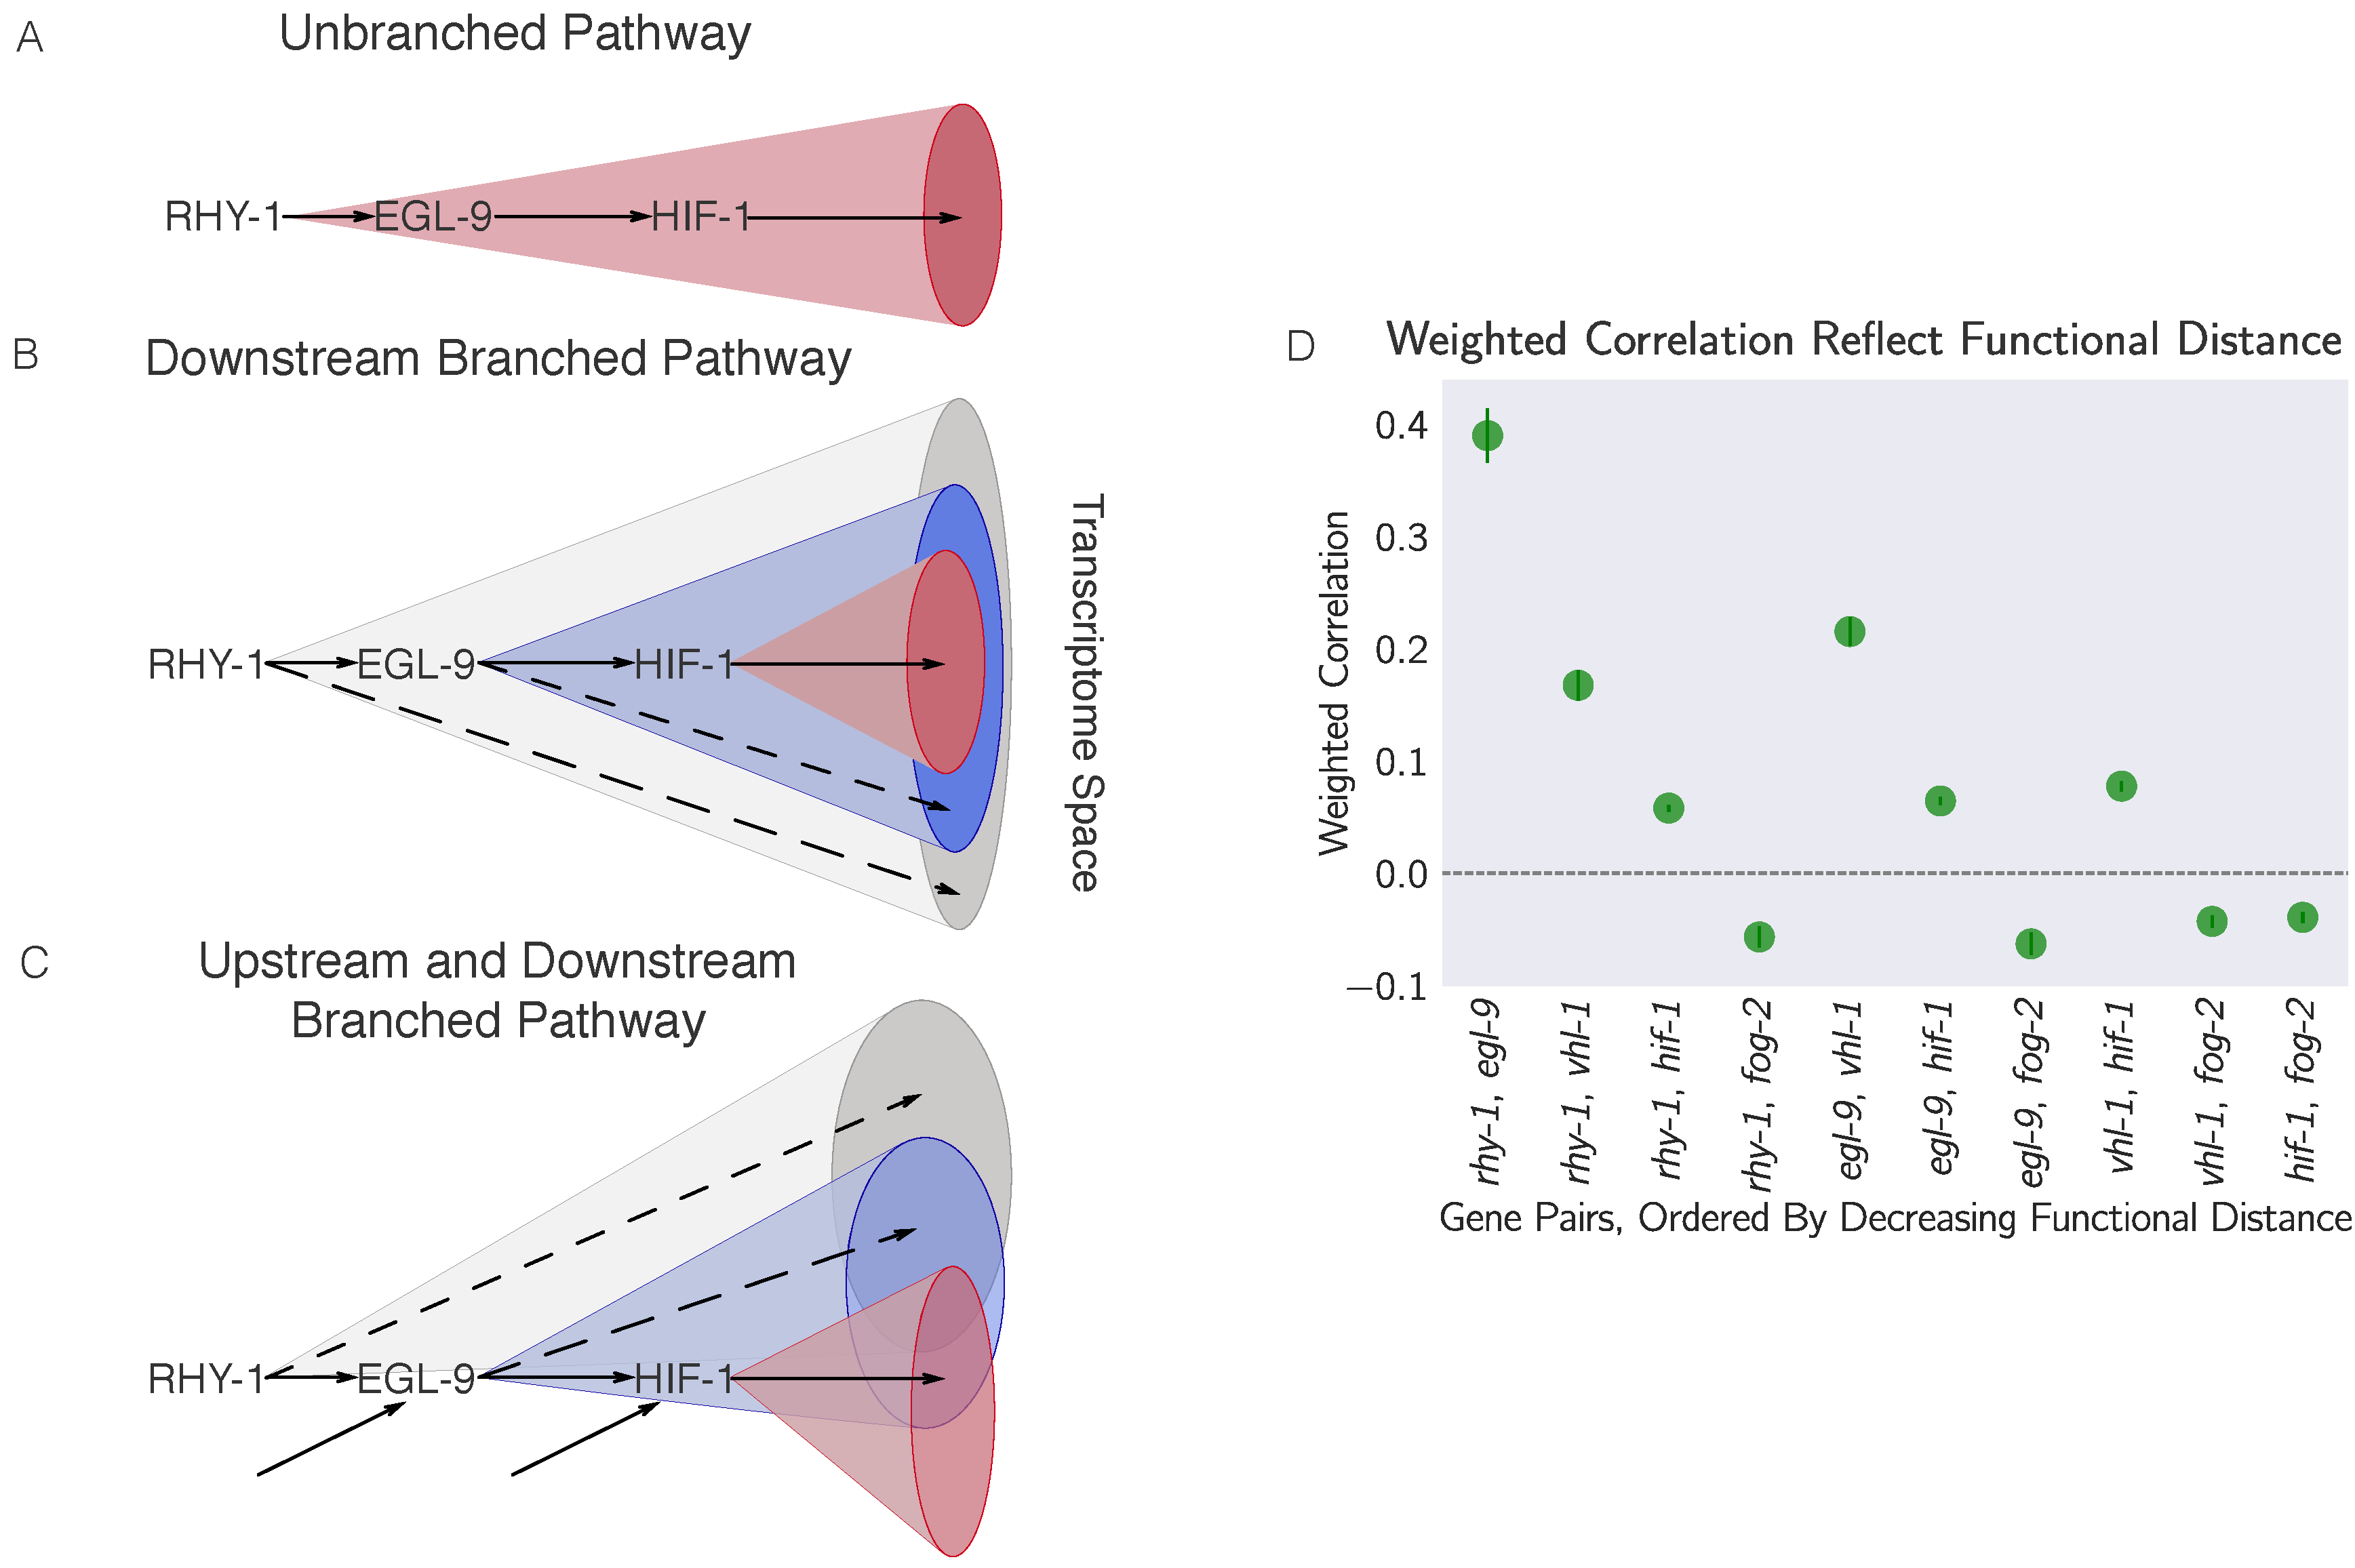
\includegraphics[width=.8\linewidth]{hypims/decorrelation-horizontal.pdf}
\caption{
Theoretically, transcriptomes can be used to order genes in a pathway under
certain assumptions. Arrows in the diagrams above are intended to show the
direction of flow, and do not indicate valence.
\textbf{A}. A linear pathway in which \gene{rhy-1} is the only gene controlling
\gene{egl-9}, which in turn controls \gene{hif-1} does not contain information
to infer the order between genes.
\textbf{B}. If \gene{rhy-1} and \gene{egl-9} have transcriptomic effects that are
separable from \gene{hif-1}, then the \gene{rhy-1} transcriptome should contain
contributions from \gene{egl-9}, \gene{hif-1} and \gene{egl-9}- and
\gene{hif-1}-independent pathways. This pathway contains enough information to
infer order.
\textbf{C}. If a pathway is branched both upstream and downstream,
transcriptomes will show even faster decorrelation. Nodes that are
separated by many edges may begin to behave almost independently of each other
with marginal transcriptomic overlap or correlation.
\textbf{D}. The hypoxia pathway can be ordered.
We hypothesize the rapid decay in correlation is due to a mixture of
upstream and downstream branching that happens along this pathway. Bars show the
standard error of the weighted coefficient from the Monte Carlo Markov Chain
computations.
}
\label{fig:decorrelation}
\end{figure}


We investigated the possibility that transcriptomic signals do in fact contain
relevant information about the degrees of separation by weighting the robust
Bayesian regression between each pair of genotypes by the size of the shared
transcriptomic phenotype of each pair divided by the total number of isoforms
differentially expressed in either mutant
($N_\mathrm{Intersection}/N_{\mathrm{Union}}$). We plotted the weighted
correlation of each gene pair, ordered by increasing functional distance
(see Fig.~\ref{fig:decorrelation}). In every case, we see that the weighted
correlation decreases monotonically due mainly, but not exclusively, to a smaller
STP.\@ We believe that this result is not due to random noise or insufficiently
deep sequencing. Instead, we propose a framework in which every gene is regulated
by multiple different molecular species, which induces progressive decorrelation.
This decorrelation in turn has two consequences. First, decorrelation within a
pathway implies that two nodes may be almost independent of each other if the
functional distance between them is large. Second, it may be possible to use
decorrelation dynamics to infer gene order in a branching pathway, as we have
done with the hypoxia pathway.

\subsection*{The circuit topology of the hypoxia pathway explains patterns in
            the data}
\label{sub:topology}
We noticed that while some of the rank plots contained a clear positive correlation
(see Fig.~\ref{fig:genetic_interactions}), other rank plots showed
a discernible cross-pattern (see Fig.~\ref{fig:xpattern}). In particular, this
cross-pattern emerged between \vhl{} and \rhy{} or between \vhl{} and \egl{},
even though genetically \gene{vhl-1}, \gene{rhy-1} and \gene{egl-9} are all
inhibitors of \hif{}. Such cross-patterns could be indicative of feedback loops
or other complex interaction patterns.

% correlative genetics again
\begin{figure}[tbhp]
\centering
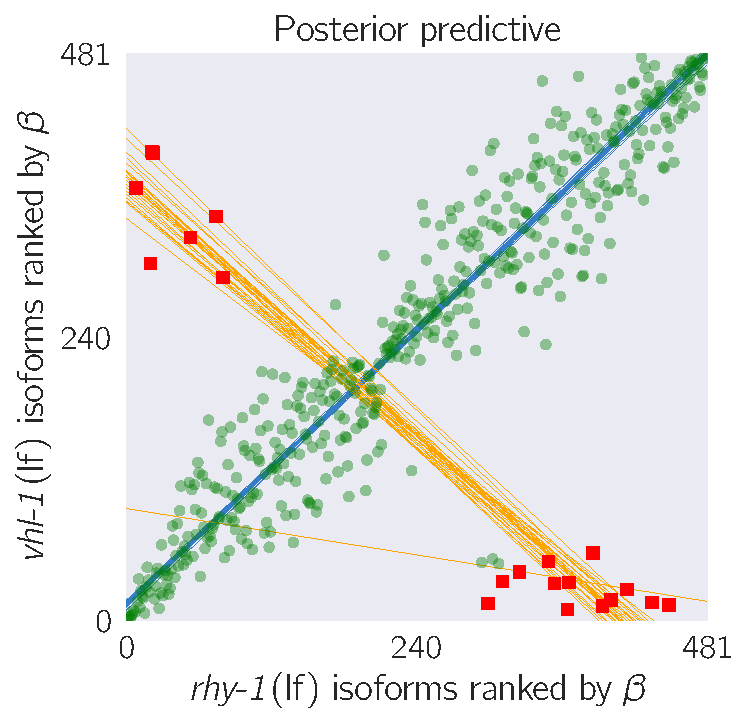
\includegraphics[width=.4\linewidth]{hypims/multiplemodes-ed.pdf}
\caption{
A feedback loop can generate transcriptomes that are both
correlated and anti-correlated. The \vhl{}/\rhy{} STP shows a cross-pattern.
Green large points are inliers to the first
regression. Red squares are outliers to the first regression. Only the red
small points were used for the secondary regression. Blue lines are representative
samples of the primary bootstrapped regression lines. Orange lines are
representative samples of the secondary bootstrapped regression lines.
}
\label{fig:xpattern}
\end{figure}



If the above is correct, then it should be possible to identify
\gene{egl-9}-independent, \rhy{}-dependent target genes in a
logically consistent way.
One erroneous way to identify these targets is via
subtractive logic. Using subtractive logic, we would identify genes that are
differentially expressed in \rhy{} mutants but not in \egl{} mutants.  Such a
gene set would
consist of almost 700 genes. One major drawback of subtractive logic is that it
cannot be applied when feedback loops exist between the genes in question.
Another problem is that the set of identified genes are statistically indistinguishable
from false positive and false negative hits because they have no distinguishing
property beyond the condition that they should be differentially expressed in
one mutant but not the other. In fact, this is exactly the behavior expected of
false-positive or false-negative hits---presence in one, but not multiple, mutants.
We need to consider the relationship between two genes before we can begin to
identify targets which expression is dependent on one gene and independent
of the other.

\gene{rhy-1} and \gene{egl-9} share a well-defined relationship. \rhyp{}
inhibits \cyslp{},
which in turn inhibits \eglp{}~\citep{Ma2012}. Therefore, loss of \rhyp{} leads
to inactivation of \eglp{}, which leads to increase in the cellular levels of
\hifp{}. \hifp{} in turn causes the mRNA levels of \gene{rhy-1} and \gene{egl-9}
to increase,
as they are involved in the \gene{hif-1}-dependent hypoxia response. However, since
\gene{rhy-1} has been mutated, the observed transcriptome is
\rhyp{} `null'; \eglp{} `null'; \hifp{} `on'. The situation is similar for
\egl{}, except that \rhyp{}
is not inactive, and therefore the observed transcriptome is the result of
\rhyp{} `up'; \eglp{} `null'; and \hifp{} `on'. From this pattern, we conclude that
the \egl{} and \rhy{} transcriptomes should exhibit a cross-pattern when plotted
against each other: The positive
arm of the cross is the result of the \eglp{} `null'; \hifp{} `on' dynamics; and the
negative arm reflects the different direction of \rhyp{} activity between
transcriptomes. No negative arm is visible (with the exception of two
outliers, which are annotated as pseudogenes in WormBase). Therefore, in this
dataset we do not find genes that have \gene{egl-9} independent,
\gene{rhy-1}-dependent expression patterns.

We also identified a main hypoxia response induced by disinhibiting
\gene{hif-1} (355 genes) by identifying genes that were commonly up-regulated
amongst \egl{}, \rhy{} and \vhl{} mutants. Although the hypoxic response is likely
to involve between three and seven times more genes (assuming the \rhy{} transcriptome
reflects the maximal hypoxic response), this is a conservative
estimate that minimizes false positive results, since these changes were
identified in four different genotypes with three replicates each. This response
included five transcription factors (\gene{W02D7.6}, \nhr{}, \gene{ztf-18},
\gene{nhr-135} and \gene{dmd-9}). The full list of genes associated with the
hypoxia response can be found in the Supplementary Table 1.
% TODO: SI numbering

\gene{hif-1}-independent effects of \gene{egl-9} have been reported
previously~\citep{Park2012}, which led us to question whether we could identify
similar effects in our dataset. We have observed that \hif{} displays a modest
increase in the transcription of \gene{rhy-1}, from which we speculated that
\eglp{} would have increased activity in the \hif{} mutant compared to the wild-type.
Therefore, we searched for genes that were regulated in an opposite manner between
\hif{} and \eglhif{}, and that were regulated in the same direction between
all \egl{} genotypes. We did not find any genes that met these conditions.

We also searched for genes with \gene{hif-1} independent, \gene{vhl-1}-dependent gene
expression and found \vhltargets{} genes, which can be found in the Supplementary
Table 2.
Finally, we searched for candidates directly regulated by \gene{hif-1}. Initially, we
searched for genes that had were significantly altered in \hif{} genotypes in one
direction, but altered in the opposite direction in mutants that activate the
\hifp{} response. Only two genes (\emph{R08E5.3}, and \emph{nit-1}) met these
conditions. This could reflect the fact that \hifp{} exists at very low
levels in \cel{}, so loss of function mutations in \gene{hif-1} might only have
mild effects on its transcriptional targets. We reasoned that genes
that are overexpressed in mutants that induce the \hifp{} response would be enriched
for genes that are direct candidates.  We found \hiftargets{}  genes which have
consistently increased expression in mutants with a constitutive hypoxic response.
These genes can be found in the Supplementary Table 3.


\subsubsection*{Enrichment analysis of the hypoxia response}
\label{sub:ea_hypoxia}
To validate that our transcriptomes were correct, and to understand how
functionalities may vary between them, we subjected each decoupled response to
enrichment analysis using the WormBase Enrichment Suite~\citep{Angeles-Albores2016,
Angeles-Albores2016b}.

\begin{figure}[tbhp]
\centering
\includegraphics[width=.7\linewidth]{hypims/hypoxia_response_gea.pdf}
\caption{
Gene ontology enrichment analysis of genes associated with the main hypoxia response.
A number of terms reflecting catabolism and bioenergetics are enriched.
}
\label{fig:hyp_gea}
\end{figure}

We used gene ontology enrichment analysis (GEA) on the main hypoxia response program.
This showed that the terms `oxoacid metabolic process' (\qval{4}, 3.0 fold-change,
24 genes), `iron ion binding' (\qval{2}, 3.8 fold-change, 10 genes), and `immune
system process' (\qval{3}, 2.9 fold-change, 20 genes) were significantly enriched.
GEA also showed enrichment of the term `mitochondrion' (\qval{3}, 2.5 fold-change,
29 genes) (see Fig.~\ref{fig:hyp_gea}). Indeed, \hif{} has been implicated in
all of these biological and molecular functions~\citep{Luhachack2012,Ackerman2012,
Romney2011,Semenza2011}.
As benchmark on the quality of our data, we selected a set of 22 genes known to
be responsive to \hifp{} levels from the literature and asked whether these genes
were present in our hypoxia response list. We found $8/22$ known genes, which
constitutes a statistically significant result ($p<10^{10}$). The small number of
reporters found in this list probably reflects the conservative nature of our
estimates.
We studied the \gene{hif-1}-independent, \gene{vhl-1}-dependent gene set
using enrichment analysis but no terms were significantly enriched.

\subsection*{Identification of non-classical epistatic interactions}
\label{sub:hifoh}
\hif{} has traditionally been viewed as existing in a genetic OFF state under
normoxic conditions. However, our dataset indicates that \hifn{} genes show
altered expression when \gene{hif-1} function is removed in normoxic conditions.
Moreover, we observed positive correlations between \hif{} $\beta$ coefficients
and \egl{}, \vhl{} and \rhy{} $\beta$ coefficients in spite of the negative
regulatory relationships between these genes and \gene{hif-1}. Such
positive correlations could indicate a different relationship between these genes
than has previously been reported, so we attempted to substantiate them through
epistasis analyses.

To perform epistasis analyses, we first identified genes that exhibited violations
of the canonical genetic model of the hypoxia pathway. To this end, we searched for
genes that exhibited different behaviors between \egl{} and \vhl{}, or
between \rhy{} and \vhl{} (we assume that all results from the
\rhy{} transcriptome reflect a complete loss of \gene{egl-9} activity). We found
\hifohtargets{} that satisfied this condition (see Fig.~\ref{fig:hif1oh},
Supplemental Table 4).
Additionally, many of these genes exhibited a new kind of epistasis. Namely,
\gene{egl-9} was epistatic over \gene{vhl-1}. Identification of a set of genes
that have a consistent set of relationships between themselves suggests that
we have identified a new aspect of the hypoxia pathway.

\begin{figure}[tbhp]
\centering
\includegraphics[width=\linewidth]{hypims/hif1oh-epistasis-horizontal.pdf}
\caption{
\textbf{A}. 27 genes in \cel{} exhibit non-classical epistasis in the hypoxia
pathway, characterized by opposite effects on gene expression, relative to the
wild-type, of of the \vhl{} compared to \egl{} (or
\rhy{}) mutants. Shown are a random selection of 15 the 27 genes for illustrative
purposes.
\textbf{B}. Representative genes showing that non-canonical epistasis shows a
consistent pattern. \vhl{} mutants have an opposite effect to \egl{}, but
\gene{egl-9} remains epistatic to \gene{vhl-1} and loss-of-function mutations in
\gene{hif-1} suppress the \egl{} phenotype. Asterisks show $\beta$ values
significantly different from 0 relative to wild-type (\qval{1}).
}
\label{fig:hif1oh}
\end{figure}

To illustrate this, we focused on three genes, \nlp{}, \ftna{} and \ftnb{}, which
epistasis patterns that we felt reflected the population well. \ftna{} and \ftnb{}
are both described in the literature as genes that are responsive to mutations in
the hypoxia pathway. Moreover, these genes have been previously described to have
aberrant behaviors~\citep{Ackerman2012,Romney2011}, specifically the
opposite effects of \egl{} and \vhl{}. These studies showed that loss of \vhl{}
decreases expression of \ftna{} and \ftnb{} using both RNAi and alleles, which
allays concerns of strain-specific interference. Moreover, Ackerman and Gems (2012)
showed that \gene{vhl-1} is epistatic to \gene{hif-1} for the \ftna{}
expression phenotype, and that loss of
\hifp{} is associated with increased expression of \ftna{} and \ftnb{}. We observed
that \gene{hif-1} was epistatic to \gene{egl-9}, and that \gene{egl-9} and
\gene{hif-1} both promoted \ftna{} and \ftnb{} expression.

Epistasis analysis of \ftna{} and \ftnb{} expression reveals that \gene{egl-9} is
epistatic to \gene{hif-1}; that \gene{vhl-1} has opposite effects to \gene{egl-9},
and that \gene{vhl-1} is epistatic to \gene{egl-9}. Analysis of \nlp{}
reveals similar relationships. \nlp{} expression is decreased in \hif{},
and increased in \egl{}. However, \gene{egl-9} is epistatic to \gene{hif-1}.
Like \ftna{} and \ftnb{}, \gene{vhl-1} has the opposite effect to \gene{egl-9},
yet is epistatic to \gene{egl-9}. We propose in the Discussion a model for how
\hifp{} might regulate these targets.

\subsection*{\hifp{} in the cellular context}
\label{sub:metabolism}

We identified the transcriptional changes
associated with bioenergetic pathways in \cel{} by extracting from
WormBase all genes associated with the tricarboxylic acid (TCA) cycle, the
electron transport chain (ETC) and with the \cel{} GO term energy reserve.
Previous research has described the effects of mitochondrial dysfunction in
eliciting the hypoxia response~\citep{Lee2010}, but transcriptional feedback
from \hifp{} into bioenergetic pathways has not been as extensively in \cel{},
as in vertebrates (see, for example~\citep{Semenza1994,Semenza2012}).
We also searched for the changes in ribosomal components and the proteasome, as
well as for terms relating to immune response (see Fig~\ref{fig:genomewide}).

\begin{figure}[tbhp]
\centering
\includegraphics[width=.7\linewidth]{hypims/hif1genomewide.pdf}
\caption{
A graphic summary of the genome-wide effects of \hifp{} from our RNA-seq data.
}
\label{fig:genomewide}
\end{figure}

\subsubsection*{Bioenergetic pathways}
Our data shows that most of the enzymes involved in the TCA cycle and in the ETC
are down-regulated when \hifp{} is induced in agreement with the previous
literature~\citep{Semenza2012}.
However, the fumarase gene \gene{fum-1} and the mitochondrial complex II stood out
as notable exceptions to the trend, as they were up-regulated in every single
genotype that causes deployment of the hypoxia response. FUM-1 catalyzes the
reaction of fumarate into malate, and complex II catalyzes the reaction of
succinate into fumarate. Complex II has been identified as a source of reserve
respiratory capacity in neonatal rat cardiomyocytes previously~\citep{Pfleger2015}.
We found two energy reserve genes that were down-regulated by \hifp{}.
\gene{aagr-1} and \gene{aagr-2}, which are predicted to function in glycogen
catabolism~\citep{Sikora2010}.
Three distinct genes involved in energy reserve were up-regulated. These genes were
\gene{ogt-1}, which encodes O-linked GlcNac Transferase gene; \gene{T04A8.7},
encoding an ortholog of human glucosidase, acid beta (GBA); and \gene{T22F3.3},
encoding ortholog of human glycogen phosphorylase isozyme in the muscle (PYGM).

\subsubsection*{Protein synthesis and degradation}
\hif{} is also known to inhibit protein synthesis and translation in varied
ways.~\citep{Brugarolas2004}. Most reported effects of
\hifp{} on the translation machinery are posttranslational, and no reports to date
show transcriptional control of the ribosomal machinery in \cel{} by \hifp{}. We
used the WormBase Enrichment Suite Gene Ontology
dictionary~\citep{Angeles-Albores2016b} to extract 143 protein-coding genes
annotated as `structural constituents of the ribosome' and we queried whether
they were differentially expressed in our mutants. \egl{}, \vhl{}, \rhy{} and
\egl{};\vhl{} showed differential expression of 91 distinct ribosomal constituents
(not all constituents were detected in all genotypes). For every one of these
genotypes, these genes were always down-regulated. In contrast, \hif{} showed
up-regulation of a single ribosomal constituent.

Next, we asked whether \hifp{} has any transcriptional effects on the
proteasomal constituents; no such effects of \hifp{} on the proteasome
have been reported in \cel{}. Out of 40 WormBase-annotated proteasomal constituents,
we found 31 constituents that were differentially expressed in at least one of the
four genotypes that induce a hypoxic response. Every gene we found was down-regulated
in at least two out of the four genotypes we studied.

\section*{Discussion}
\subsection*{The \cel{} hypoxia pathway can be reconstructed entirely from
             RNA-seq data}
In this paper, we have shown that whole-organism transcriptomic phenotypes
can be used to reconstruct genetic pathways and to discern previously overlooked
or uncharacterized genetic interactions. We successfully reconstructed the hypoxia
pathway, and inferred order of action (\gene{rhy-1} activates \gene{egl-9},
\gene{egl-9} and \gene{vhl-1} inhibit \gene{hif-1}), and we were able to infer
from transcriptome-wide epistasis measurements that \gene{egl-9} exerts
\gene{vhl-1}-dependent and independent inhibition on \gene{hif-1}.

\subsection*{\hifp{} and the cellular environment}

In addition to reconstructing the pathway, our dataset allowed us
to observe a wide variety of physiologic changes that occur as a result of the
\hifp{}-dependent hypoxia response. In particular, we observed down-regulation of most
components of the TCA cycle and the mitochondrial electron transport chain with
the exceptions of \gene{fum-1} and the mitochondrial complex II.\@ The mitochondrial
complex II catalyzes the reaction of succinate into fumarate.
In mouse embryonic fibroblasts, fumarate has been
shown to antagonize \hifp{} prolyl hydroxylase domain (PHD) enzymes, which are
orthologs of \eglp{}~\citep{Sudarshan2009}.
If the inhibitory role of fumarate on PHD enzymes is conserved in \cel{},
upregulation of complex II by \hifp{} during hypoxia may increase
intracellular levels of fumarate, which in turn could lead to artificially high
levels of \hifp{}
even after normoxia resumes. The increase in fumarate produced by the complex
could be compensated by increasing expression of \gene{fum-1}. Increased fumarate
degradation allows \cel{} to maintain plasticity in the hypoxia pathway, keeping
the pathway sensitive to oxygen levels.

\subsection*{Interpretation of the non-classical epistasis in the hypoxia pathway}
The observation of almost 30 genes that exhibit a specific pattern of non-classical
epistasis suggests the existence of previously undescribed aspects of the hypoxia
pathway. Some of these non-classical epistases had been observed
previously~\citep{Ackerman2012,Romney2011,Luhachack2012}, but
no satisfactory mechanism has been proposed to explain this biology.
\citet{Romney2011} and \citet{Ackerman2012}
suggest that \hifp{} integrates information on iron concentration in the
cell to bind to the \ftna{} promoter, but could not definitively establish
a mechanism.
It is unclear why deletion of \gene{hif-1} induces \ftna{}
expression, deletion of \gene{egl-9} also causes induction of \ftna{} expression,
but deletion of \gene{vhl-1} removes this inhibition. Moreover, \citet{Luhachack2012}
have previously reported that certain genes important for the \cel{} immune response
against pathogens reflect similar expression patterns. Their interpretation
was that \gene{swan-1}, which encodes a binding partner to \eglp{}~\citep{Shao2010},
is important for modulating \hifp{} activity in some manner. The lack of a
conclusive double mutant analysis in this work means the role of SWAN-1 in
modulation of \hifp{} activity remains to be demonstrated. Nevertheless, mechanisms
that call for additional transcriptional modulators become less likely given the
number of genes with different biological functions that exhibit the same pattern.

\begin{figure}[tbhp]
\centering
\includegraphics[width=.5\linewidth]{hypims/hif1oh_model.pdf}
\caption{
A hypothetical model showing a mechanism where \hifp{}-hydroxyl antagonises
\hifp{}.
\textbf{A}. Diagram showing that RHY-1 activates EGL-9.
EGL-9 hydroxylates HIF-1 in an oxygen dependent fashion. Under normoxia, HIF-1
is rapidly hydroxylated and only slowly does hydroxylated HIF-1 return to its
original state. EGL-9 can also inhibit HIF-1 in an oxygen-independent fashion.
HIF-1 hydroxyl is rapidly degraded in a VHL-1 dependent fashion. In our model,
HIF-1 and HIF-1 hydroxyl have opposing effects on transcription. The width of the
arrows represents the rates under normoxic conditions.
\textbf{B}. Table showing the effects of loss-of-function mutations on HIF-1 and
HIF-1 hydroxyl activity, showing how this can potentially explain the behavior
of \gene{ftn-1} in each case.  S.S = Steady-state.
}
\label{fig:hif1oh_table}
\end{figure}

One way to resolve this problem without invoking additional genes is to
consider \hifp{} as a protein with both activating and inhibiting states. In fact,
\hifp{} already exists in two states in \cel{}: unmodified \hifp{} and
\hifp{}-hydroxyl (\hifp{}-OH). Under this model, \hifp{}-hydroxyl antagonizes
the effects of \hifp{} for certain genes like \ftna{} or \nlp{}. Loss of
\gene{vhl-1} stabilizes \hifp{}-hydroxyl.
A subset of genes that are sensitive to \hifp{}-hydroxyl will be inhibited as a
result of the increase in the amount of this species, in spite of loss of
\gene{vhl-1} function also increasing the level of non-hydroxylated \hifp{}.
On the other hand, \egl{} selectively removes all \hifp{}-hydroxyl, stimulating
accumulation of \hifp{} and promoting gene activity. Whether deletion of \hif{}
is overall activating or inhibiting will depend on the relative activity of each
protein state under normoxia (see Fig.~\ref{fig:hif1oh_table}).

Multiple lines of circumstantial evidence that \hifp{}-hydroxyl plays a role
in the functionality of the hypoxia pathway. First, \hifp{}-hydroxyl is
challenging to study genetically because no mimetic mutations are available with
which to study the pure hydroxylated \hifp{} species. Second, although mutations in
the Von-Hippel Landau gene stabilize the hydroxyl species, they also increase the
quantity of non-hydroxylated \hifp{} by mass action.
Finally, since \hifp{} is detected low levels
in cells under normoxic conditions~\citep{Wang1993}, total \hifp{} protein
(unmodified \hifp{} plus \hifp{}-hydroxyl) is often tacitly assumed to be
vanishingly rare and therefore biologically inactive.

Our data show hundreds of genes that change expression in response
to loss of \gene{hif-1} under normoxic conditions. This establishes that there is
sufficient total \hifp{} protein to be biologically active.
Our analyses also revealed that \hif{} shares
positive correlations with \egl{}, \rhy{} and \vhl{}, and that each of these genotypes
also shows a secondary negative rank-ordered expression correlation with each other.
These cross-patterns between all loss of function of inhibitors of \hifp{} and
\hif{} can be most easily explained if \hifp{}-hydroxyl is biologically active.

A homeostatic argument can be made in favor of the activity of \hifp{}-hydroxyl.
At any point in time, the cell must measure the levels of
multiple metabolites at once. The \gene{hif-1}-dependent hypoxia
response integrates information from O$_2$, $\alpha$-ketoglutarate
(2-oxoglutarate) and iron concentrations in the cell. One way to
integrate this information is by encoding it only in the effective hydroxylation
rate of \hifp{} by \eglp{}. Then the dynamics in this system will evolve
exclusively as a result of the total amount of \hifp{} in the cell. Such a system
can be sensitive to fluctuations in the absolute concentration of
\hifp{}~\citep{Goentoro2009a}. Since the absolute levels of \hifp{} are low in
normoxic conditions, small fluctuations in protein copy-number represent can
represent a large fold-change in \hifp{} levels. These fluctuations would
not be problematic for genes that must be turned on only under conditions of severe
hypoxia---presumably, these genes would be associated with low affinity
sites for \hifp{}, so that they are only activated when \hifp{} levels are far
above random fluctuations.

For yet other sets of genes that must change expression in response to the hypoxia
pathway, it may not make as much sense to integrate metabolite information
exclusively via \eglp{}-dependent hydroxylation of \hifp{}. In particular, genes
that may function to increase survival in mild hypoxia may benefit from regulatory
mechanisms that can sense minor changes in environmental conditions and which
therefore benefit from robustness to transient changes in protein copy number.
Likewise, genes that are involved in iron or $\alpha$-ketoglutarate metabolism
(such as \ftna{}) may benefit from being able to sense, accurately, small and
consistent deviations from basal concentrations of these metabolites. For these
genes, the information may be better encoded by using \hifp{} and
\hifp{}-hydroxyl as an activator/repressor pair. Such circuits are
known to possess distinct advantages for controlling output in a manner that
is robust to transient fluctuations in the levels of their
components~\citep{Hart2012,Hart2013}.

Our RNA-seq data suggests that one of these atypical targets of \hifp{}
may be \rhyp{}. Although \gene{rhy-1} does not exhibit non-classical
epistasis, \hif{} and \eglhif{} both had increased expression levels of \gene{rhy-1}.
We speculate that if \gene{rhy-1} is controlled by both \hifp{} and \hifp{}-hydroxyl,
then this might imply that \hifp{} regulates the expression of its pathway (and
therefore itself) in a manner that is robust to total \hifp{} levels.

\subsection*{Insights into genetic interactions from vectorial phenotypes}

Here, we have described a set of straightforward methods that can be in theory
applied to any vectorial phenotype. Genome-wide methods afford a lot of information,
but genome-wide interpretation of the results is often extremely challenging.
Each method has its own advantages and disadvantages. We briefly discuss these
methods, their uses and their drawbacks.

Principal component analysis
is computationally tractable and clusters can often be visually detected with
ease. However, PCA can be misleading, especially when the dimensions represented
do not explain a very large fraction of the variance present in the data. In addition,
principal dimensions are the product of a linear combination of vectors, and therefore
must be interpreted with extreme care. In this case, the first principal dimension
separated genotypes that increase \hifp{} protein levels from those that decrease
it, but this dimension is a mix of vectors of change in gene expression. Although
PCA showed that there is information hidden in these genotypes, it was not enough
by itself to provide biological insight.

Whereas PCA operates on all genotypes simultaneously, correlation analysis is a
pairwise procedure that measures how predictable the gene
expression changes are in a mutant given the vector of expression changes in
another. Like PCA, correlation analysis is easy and fast to perform. Unlike PCA,
the product of a correlation analysis is a single number with a straightforward
interpretation. However, correlation analysis is particularly sensitive to outliers.
Although a common strategy is to rank-transform expression data to mitigate
outliers, rank-transformations do not remove the cross-patterns that appear when
feedback loops or other complex interactions are present between two genes.
Such cross-patterns can still lead to vanishing correlations if both patterns are
equally strong. Therefore, correlation analyses must take into account the possible
existence of systematic outliers. Moreover, correlation values must be measured
for both interactions in cross-patterned rank plots. Weighted correlations could
be informative for ordering genes along pathways.
A drawback of correlation
analysis is that the number of pairwise comparisons that must be made increases
combinatorially, though strategies could be used to decrease the total number of
effective comparisons.

Epistasis plots are a novel way to visualize epistasis in vectorial phenotypes.
Here, we have shown how an epistasis plot can be used to identify interactions
between two single mutants and a double mutant. In reality, epistasis plots
can be generated for any set of measurements involving a set of $N$ mutants and
an $N$-mutant genotype. Epistasis plots can accumulate an arbitrary number of
points within them, possess a rich structure that can be visualized and have
straightforward interpretations for special slope values.

Another way to analyze epistasis is via general linear models (GLMs) that include
interaction terms between two or more genes. In this way, GLMs can quantify
the epistatic effect of an interaction on single genes. We and
others~\citep{Dixit2016,Angeles-Albores2016a} have previously used GLMs to identify
gene sets that are epistatically regulated by two or more inputs. While powerful,
GLMs suffer from the multiple comparison problem. Correcting for false positives
using well-known multiple comparison corrections such as FDR~\citep{Storey2003}
tends to increase false negative rates.  Moreover, since GLMs attempt to estimate
effect magnitudes for individual gene or isoform expression levels, they
effectively treat each gene as an independent quantity, which prevents better
estimation of the magnitude and direction of the epistasis between two genes.

Epistasis plots do not suffer from the multiple comparison problem because the
number of tests performed is orders of magnitudes smaller than the number
of tests performed by GLMs. Ideally, in an epistasis plot we need only perform
3 tests---rejection of additive, unbranched and suppressive null models---compared
with the tens of thousands of tests that are performed in GLMs. Moreover, the
magnitude of epistasis between two genes can be estimated using hundreds of genes,
which greatly improves the statistical resolution of the epistatic coefficient.
This increased resolution is important because the size and magnitude of the
epistasis has specific consequences for the type of pathway that is expected.

Any quantitative use of genome-wide datasets requires a good experimental setup.
Here, we have demonstrated that whole-organism RNA-seq can be used to dissect
molecular pathways in exquisite detail when paired with experimental designs that
are motivated by classical genetics. Much more research will be necessary
to understand whether epistasis has different consequences in the microscopic
realm of transcriptional phenotypes than in the macroscopic world that geneticists
have explored previously. Our hope is that these tools, coupled with the classic
genetics experimental  designs, will reveal hitherto unknown aspects of genetics
theory.

\section*{Methods}
\label{sec:methods}
\subsection*{Nematode strains and culture}
Strains used were N2 wild-type Bristol,
CB5602 \gene{vhl-1}(\emph{ok161}),
CB6088 \gene{egl-9}(\emph{sa307})~\gene{hif-1}(\emph{ia4}),
CB6116 \gene{egl-9}(\emph{sa307});\gene{vhl-1}(\emph{ok161}),
JT307 \gene{egl-9}(\emph{sa307}),
ZG31 \gene{hif-1}(\emph{ia4}),
RB1297 \gene{rhy-1}(\emph{ok1402}).
All lines were grown on standard
nematode growth media (NGM) plates seeded with OP50 \ecol{} at 20\degree{}C
(Brenner 1974).

\subsection*{RNA Isolation}
Unsynchronized lines were grown on NGM plates at 20C and eggs harvested by
sodium hypochlorite treatment. Eggs were plated on 6 to 9 6cm NGM plates
with ample OP50 \ecol{} to avoid starvation and grown at
20\degree{}C.  Worms were staged and harvested based on the time after plating,
vulva morphology and the absence of eggs.  Approximately 30--50 non-gravid young
adults were picked and placed in 100$\mu$L of TE pH 8.0 at 4\degree{}C in
$0.2$mL PCR tubes.   After settling and a brief spin in microcentrifuge
approximately $80\mu$L of TE (Ambion AM 9849) was removed from the top of the
sample and individual replicates
were snap frozen in liquid N2. These replicate samples were then digested with
Proteinase K (Roche Lot No. 03115 838001 Recombinant Proteinase K PCR Grade) for
15min at 60\degree{} in the presence of 1\% SDS and 1.25$\mu$L
RNA Secure (Ambion AM 7005). RNA samples were then taken up in 5 Volumes of
Trizol (Tri Reagent Zymo Research) and processed and treated with DNase I using
Zymo MicroPrep RNA Kit (Zymo Research Quick-RNA MicroPrep R1050).
RNA was eluted in RNase-free water and divided into aliquots and stored at
-80\degree{}C. One aliquot of each replicate was analyzed using a NanoDrop (Thermo
Fisher) for impurities, Qubit for concentration and then analyzed on an Agilent
2100 BioAnalyzer (Agilent Technologies).
Replicates were selected that had RNA integrity numbers (RIN) equal or greater
than 9.0 and showed no evidence of bacterial ribosomal bands, except for the
ZG31 mutant where one of three replicates had a RIN of 8.3.

\subsection*{Library Preparation and Sequencing}
10ng of quality checked total RNA from each sample was
reverse-transcribed into cDNA using the Clontech SMARTer Ultra Low Input RNA for
Sequencing v3 kit (catalog \#634848) in the SMARTSeq2 protocol
~\citep{Picelli2014}.  RNA was denatured at 70$\degree{}$C for 3 minutes
in the presence of dNTPs, oligo dT primer and spiked-in quantitation standards
(NIST/ERCC from Ambion, catalog \#4456740).  After chilling to 4$\degree{}$C, the
first-strand reaction was assembled using the LNA TSO primer described in
\citet{Picelli2014}, and run at 42$\degree{}$C for 90 minutes, followed by
denaturation at 70$\degree{}$C for 10 minutes.  The entire first strand reaction
was then used as template for 13 cycles of PCR using the Clontech v3 kit.
Reactions were cleaned up with 1.8X volume of Ampure XP SPRI beads (catalog
\#A63880) according to the manufacturer’s protocol.  After quantification using
the Qubit High Sensitivity DNA assay, a 3ng aliquot of the amplified cDNA was
run on the Agilent HS DNA chip to confirm the length distribution of the
amplified fragments.  The median value for the average cDNA lengths from all
length distributions was 1076bp.  Tagmentation of the full length cDNA for
sequencing was performed using the Illumina/Nextera DNA library prep kit (catalog
\#FC-121--1030).  Following Qubit quantitation and Agilent BioAnalyzer profiling,
the tagmented libraries were sequenced. Libraries were sequenced on Illumina
HiSeq2500 in single read mode with the read length of 50nt to an average depth
of 15 million reads per sample following manufacturer's instructions. Base calls
were performed with RTA 1.13.48.0 followed by conversion to FASTQ with bcl2fastq
1.8.4. Spearman correlation of the transcripts per million (TPM) for each
genotype showed that every pairwise correlation within genotype was $>0.9$.

\subsection*{Read Alignment and Differential Expression Analysis}
We used Kallisto to perform read pseudo-alignment and performed differential
analysis using Sleuth. We fit a general linear model for a transcript $t$ in
sample $i$:

\begin{equation}
  y_{t,i} = \beta_{t, 0} + \beta_{t, genotype}\cdot{}X_{t, i} +
  \beta_{t, batch}\cdot{}Y_{t, i} + \epsilon_{t, i}
\end{equation}

where $y_{t, i}$ are the logarithm transformed counts; $\beta_{t, genotype}$ and
$\beta_{t, batch}$ are parameters of the model, and which can be interpreted as
biased estimators of the log-fold change; $X_{t, i}, Y_{t, i}$ are indicator
variables describing the conditions of the sample; and $\epsilon_{t, i}$ is the
noise associated with a particular measurement.

\subsection*{Genetic Analysis, Overview}
Genetic analysis of the processed data was performed in Python 3.5. Our scripts
made extensive use of the Pandas, Matplotlib, Scipy, Seaborn, Sklearn, Networkx,
Bokeh, PyMC3, and TEA libraries~\citep{Team2014,McKinney2011,Oliphant2007,
Pedregosa2012,Salvatier2015,VanDerWalt2011,Hunter2007,Angeles-Albores2016,Waskom}.
Our analysis is available in a Jupyter Notebook~\citep{Perez2007}. All code and
required data (except the raw reads) are available at
\url{https://github.com/WormLabCaltech/mprsq} along with version-control
information. Our Jupyter Notebook and interactive graphs for this project can be
found at \url{https://wormlabcaltech.github.io/mprsq/}. Raw reads were deposited
in the Short Read Archive under the study accession number SRP100886.


\subsection*{Weighted Correlations}
Pairwise correlations between transcriptomes where calculated by first identifying
the set of differentially expressed genes (DEGs) common to both transcriptomes under
analysis. DEGs were then rank-ordered according to their regression coefficient,
$\beta$.\ Bayesian robust regressions were performed using a Student-T distribution.
Bayesian analysis was performed using the PyMC3 library~\citep{Salvatier2015}
(\texttt{pm.glm.families.StudenT} in Python). If the correlation has an average
value $>1$, the correlation coefficient was set to 1.

Weights were calculated as the proportion of genes that were $<1.5$ standard
deviations away from the primary regression out of the entire set of shared DEGs
for each transcriptome.

\subsection*{Epistasis Analysis}
For a double mutant $X^-Y^-$, we used the single mutants $X^-$ and $Y^-$ to
find expected value of the coefficient for a double mutant under an additive model
for each isoform $i$.
Specifically,
\begin{equation}
  \beta_{\mathrm{Add},i} = \beta_{X,i} + \beta_{Y,i}.
\end{equation}

Next, we find the difference, $\Delta_i$, between the observed double mutant
expression coefficient, $\beta_{XY, \mathrm{Obs},i}$, and the predicted
expression coefficient under an additive model for each isoform $i$.

To calculate the transcriptome-wide epistasis coefficient, we plotted
($\beta_{\mathrm{Add},i}, \Delta_i$) and found the line of best fit using
orthogonal distance regression using the \texttt{scipy.odr} package in Python.
We performed
non-parametric bootstrap sampling of the ordered tuples with replacement using
5,000 iterations to generate a probability distribution of slopes of best fit.

There are as many models as epistatic relationships. For quantitative phenotypes,
epistatic relationships (except synthetic interactions) can be generally
expressed as:

\begin{equation}
  \beta_{XY} = \sum_{g\in G} \lambda_g \beta_g,
  \label{eq:epi}
\end{equation}

where $P_i$ is the quantitative phenotype belonging to the genotype $i$; $G$ is
the set of single mutants $\{X, Y\}$ that make up the double mutant, $XY$; and
$\lambda_g$ is the contribution of the phenotype $P_g$ to $P_{XY}$.
Additive interactions between genes are the result of setting $\lambda_g=1$. All
other relationships correspond to setting  $\lambda_X=0,~\lambda_Y=1$ or
$\lambda_X=1,~\lambda_Y=0$.

A given epistatic interaction can be simulated by predicting the double mutant
phenotype under that interaction and re-calculating the y-coordinates. The
recalculated y-coordinates can then be used to predict the possible epistasis
coefficients for the cases where $X$ is epistatic over $Y$, and $Y$ is epistatic
over $X$.

To select between theoretical models, we implemented an approximate Bayesian
Odds Ratio. We defined a free-fit model, $M_1$, that found the line of best fit
for the data:

\begin{equation}
  P(\alpha~|M_1, D) \propto \prod_{(x_i, y_i, \sigma_i)\in D}
  \exp{\frac{
            (y_i - \alpha\cdot x_i)^2
            } % numerator
            {
            2\sigma_i
            } % denominator
            } \cdot (1+\alpha^2)^{-3/2},
  \label{eq:free_model}
\end{equation}

where $\alpha$ is the slope of the model to be determined, $x_i, y_i$ were the
x- and y-coordinates of each point respectively, and $\sigma_i$ was the standard
error associated with the y-value. We minimized the
negative logarithm of equation~\ref{eq:free_model} to obtain the most likely
slope given the data, $D$ (\texttt{scipy.optimize.minimize} in Python). Finally,
we approximated the odds ratio as:

\begin{equation}
  OR = \frac{
  P(D~|\alpha^*, M_1)\cdot (2\pi)^{1/2}\sigma_{\alpha^*} % numerator
  }{P(D~| M_i)}, % denominator
\end{equation}

where $\alpha^*$ is the slope found after minimization, $\sigma_\alpha^*$ is the
standard deviation of the parameter at the point $\alpha^*$ and $P(D~|M_i)$ is the
probability of the data given the parameter-free model, $M_i$.

\subsection*{Enrichment Analysis}
Tissue, Phenotype and Gene Ontology Enrichment Analysis were carried out using
the WormBase Enrichment Suite for Python~\citep{Angeles-Albores2016b,
Angeles-Albores2016}.



\subsubsection*{Author Contributions:}
This work was supported by HHMI with whom PWS is an investigator
and by the Millard and Muriel Jacobs Genetics and Genomics Laboratory at
California Institute of Technology.
All strains were provided by the CGC, which is funded by NIH Office of Research
Infrastructure Programs (P40 OD010440).
This article was written with support of the Howard Hughes Medical Institute.
This article wouldn't be possible without help from Dr.\_ Igor Antoshechkin who
performed all sequencing.
We thank Hillel Schwartz for all of his careful advice.
We would like to thank Jonathan Liu, Han Wang, and Porfirio Quintero for helpful
discussion.

  % \printbibliography[heading=subbibliography]
\end{refsection}

\chapter{Structural genes have transcriptional consequences}
\begin{refsection}
  % \newcommand{\dicty}{\emph{D.~discoideum}}

% gene names
\newcommand{\nlp}{\emph{\mbox{nlp-31}}}
\newcommand{\ftna}{\emph{\mbox{ftn-1}}}
\newcommand{\ftnb}{\emph{\mbox{ftn-2}}}
\newcommand{\cysl}{\emph{\mbox{cysl-1}}}
\newcommand{\nog}{\emph{\mbox{nog-1}}}
\newcommand{\nhr}{\emph{\mbox{nhr-57}}}
\newcommand{\lam}{\emph{\mbox{lam-3}}}

\newcommand{\fog}{\emph{\mbox{fog-2(lf)}}}
\newcommand{\egl}{\emph{\mbox{egl-9}(lf)}}
\newcommand{\rhy}{\emph{\mbox{rhy-1}(lf)}}
\newcommand{\vhl}{\emph{\mbox{vhl-1}(lf)}}
\newcommand{\eglvhl}{\emph{\mbox{egl-9(lf);vhl-1(lf)}}}
\newcommand{\eglhif}{\emph{\mbox{egl-9(lf)}~\mbox{hif-1(lf)}}}
\newcommand{\hif}{\emph{\mbox{hif-1(lf)}}}

% protein names
\newcommand{\eglp}{EGL-9}
\newcommand{\rhyp}{RHY-1}
\newcommand{\nogp}{NOG-1}
\newcommand{\vhlp}{VHL-1}
\newcommand{\hifp}{HIF-1}
\newcommand{\fogp}{FOG-2}
\newcommand{\nhrp}{NHR-57}
\newcommand{\lamp}{LAM-3}
\newcommand{\cyslp}{CYSL-1}

% DE genes numbers:
\newcommand{\egln}{1,806}
\newcommand{\rhyn}{2,103}
\newcommand{\vhln}{689}
\newcommand{\eglvhln}{2,376}
\newcommand{\hifn}{546}
\newcommand{\eglhifn}{404}
\newcommand{\fogn}{2090}
\newcommand{\total}{5,671} % isoforms!!!!
% \newcommand{\inall}{53}
% \newcommand{\allup}{10}
% \newcommand{\alldown}{13}

% downstream targets
\newcommand{\egltargets}{126}
\newcommand{\rhytargets}{0}
\newcommand{\vhltargets}{45} % 44 genes, minus vhl-1 (IDed due to deletion)
\newcommand{\hiftargets}{195}
\newcommand{\hifohtargets}{31}


% website commands
\newcommand{\website}{
            \url{https://wormlabcaltech.github.io/Angeles_Leighton_2016/}
            }
\newcommand{\webref}{
\href{https://wormlabcaltech.github.io/Angeles_Leighton_2016/}{website}}

% more space between rows
\newcommand{\ra}[1]{\renewcommand{\arraystretch}{#1}}

\section*{Abstract}
\textbf{
RNA-seq is commonly used to identify genetic modules that respond to perturbations.
In single cells, transcriptomes have been used as phenotypes, but this concept
has not been applied to whole-organism RNA-seq. Linear models can quantify
expression effects of individual mutants and identify epistatic effects in double
mutants. However, interpreting these high-dimensional measurements is unintuitive.
We developed a single coefficient to quantify transcriptome-wide epistasis which
accurately reflects the underlying interactions. To demonstrate the power of our
approach, we sequenced four single and two double C. elegans mutants. From these
mutants, we successfully reconstructed the known hypoxia pathway. Using this
approach, we uncovered a class of 31 genes that have opposing changes in expression
in \egl{} and \vhl{} but the \eglvhl{} mutant phenocopies \egl{}.
These changes violate the classical model of HIF-1 regulation, but can be explained
by postulating a role of hydroxylated HIF-1 in transcriptional control.
}
\vspace{10mm}


\section*{Introduction}
\label{sec:introduction}
Genetic analysis of molecular pathways has traditionally been performed
through epistatis analysis. Generalized epistasis indicates that two genes interact
functionally; such interaction can involve the direct interaction of their
products or the interaction of any consequence of their function (small molecules,
physiological or behavioral effects)~\citep{Huang2006}. If two
genes interact, and the mutants of these genes have a quantifiable phenotype,
the double mutant of interacting genes will have a phenotype that is not the sum
of the phenotypes of the single mutants that make up its genotype. Epistasis
analysis remains a cornerstone of genetics today~\citep{Phillips2008}.


Recently, biological studies have shifted in focus from studying single
genes to studying all genes in parallel. In particular,
RNA-seq~\citep{Mortazavi2008} enables biologists to
identify genes that change expression in response to a perturbation. Gene expression
profiling using RNA-seq has become much more sensitive thanks to deeper and more
frequent sequencing due to lower sequencing costs~\citep{Metzker2010},
better and faster abundance quantification~\citep{Patro2014,Bray2016,Patro2015},
and improved differential expression analysis
methods~\citep{Pimentel2016,Trapnell2013}. RNA-seq has been
successfully used to identify genetic modules involved in a variety of processes,
including T-cell regulation~\citep{Singer2016,Shalek2013}, the
\emph{Caenorhabditis~elegans} (\cel{}) linker
cell migration~\citep{Schwarz2012}, and planarian stem cell
maintenance~\citep{VanWolfswinkel2014,Scimone2014}. For the most part, the role of
transcriptional profiling has been restricted to target gene identification.

Although transcriptional profiling has been primarily used for descriptive purposes,
transcriptomic phenotypes have previously been used to make genetic inferences.
Microarray analyses in \emph{S. cerevisiae} and \dicty{} were used to show
that transcriptomes can be interpreted to infer genetic relationships in simple
eukaryotes~\citep{Hughes2000, VanDriessche2005}.\@ eQTL studies in
many organisms, from yeast to humans, have established the usefulness of
transcriptomic phenotypes for population genetics studies~\citep{Brem2002,Schadt2003,
Li2006,King2014}. In cell culture, single-cell RNA-seq has seen significant
progress towards using transcriptomes as phenotypes with which to test genetic
interactions~\citep{Adamson2016,Dixit2016}.
More recently, we have identified a new developmental state
of \cel{} using whole-organism transcriptome profiling~\citep{Angeles-Albores2016a}.
To investigate the ability of whole-organism transcriptomes to serve as quantitative
phenotypes for epistasis analysis in metazoans, we sequenced the transcriptomes of
of four well-characterized loss of function mutants in the \cel{} hypoxia
pathway~\citep{Epstein2001,Shen2006,Shao2009,Jiang2001}.

% carmie:
Metazoans depend on the presence of oxygen in sufficient concentrations to
support aerobic metabolism. Genetic pathways evolved to rapidly respond to any
acute or chronic changes in oxygen levels at the cellular or organismal level.
Biochemical and genetic approaches identified the Hypoxia Inducible Factors
(HIFs) as an important group of oxygen-responsive genes that are involved in a
broad range of human pathologies~\citep{Semenza2012}.

Hypoxia Inducible Factors are highly conserved in metazoans~\citep{Loenarz2011}.
A common mechanism for hypoxia-response induction is heterodimerization between a
HIF$\alpha$ and a HIF$\beta$ subunit; the heterodimer then initiates
transcription of target genes~\citep{Jiang1996}. The number and complexity of
HIFs varies throughout metazoans, with humans having three HIF$\alpha$ subunits
and two HIF$\beta$ subunits, whereas in the roundworm \cel{} there is a single
HIF$\alpha$ gene, \gene{hif-1}~\citep{Jiang2001} and a single HIF$\beta$
gene, \gene{ahr-1}~\citep{Powell-Coffman1998}. HIF target genes have been implicated
in a wide variety of cellular and extracellular processes including glycolysis,
extracellular matrix modification, autophagy and immunity~\citep{Semenza1994,
Bishop2004,Shen2005,Bellier2009,Semenza2012}.

Levels of HIF$\alpha$ proteins tend to be tightly regulated. Under conditions of
normoxia, \hifp{}$\alpha$ exists in the cytoplasm and partakes in a futile cycle
of continuous protein production and rapid degradation~\citep{Huang1996}.
\hifp{}$\alpha$ is hydroxylated by three proline hydroxylases
in humans (PHD1, PHD2 and PHD3) but is only hydroxylated by one proline
hydroxylase (\eglp{}) in \cel{}~\citep{Kaelin2008}. \hifp{} hydroxylation
increases its binding affinity to Von Hippel Lindau Tumor Suppressor 1
(\vhlp{}), which allows ubiquitination of \hifp{} leading to its subsequent
degradation. In \cel{}, \eglp{} activity is inhibited by binding of \cyslp{},
and \cyslp{} activity is in turn inhibited at the protein level by \rhyp{},
possibly by post-translational modifications to \cyslp{}~\citep{Ma2012} (see
Fig.~\ref{fig:pathway}).

% heatmap
\begin{figure}[tbhp]
\centering
\includegraphics[width=.7\linewidth]{hypims/HIF1pathway.pdf}
\caption{
Genetic and biochemical representation of the hypoxia pathway in \cel{}.
Red arrows are arrows that lead to inhibition of \hifp{}, and blue arrows
are arrows that increase \hifp{} activity or are the result of \hifp{} activity.
\eglp{} is known to exert \gene{vhl-1}-dependent and independent repression
on \hifp{} as shown in the genetic diagram. The \gene{vhl-1}-independent
repression of \hifp{} by \eglp{} is denoted by a dashed line and is not dependent
on the hydroxylating activity of \eglp{}.
Technically, RHY-1 inhibits CYSL-1, which in turn inhibits EGL-9, but this
interaction was abbreviated in the genetic diagram for clarity.
}
\label{fig:pathway}
\end{figure}

Here, we show that transcriptomes contain robust signals that can be
used to infer relationships between genes in complex metazoans by reconstructing
the hypoxia pathway in \cel{} using RNA-seq.
Furthermore, we show that the phenomenon of phenotypic epistasis, a hallmark of
genetic interaction, holds at the molecular systems level.
We also demonstrate that transcriptomes contain sufficient information, under
certain circumstances, to order genes in a pathway using only single mutants.
Finally, we were able to identify genes that appear to be downstream of \gene{egl-9}
and \gene{vhl-1}, but do not appear to be targets of \gene{hif-1}.
Using a single set of genome-wide measurements, we were able to observe and
quantitatively assess  significant fraction of the known transcriptional
effects of \gene{hif-1} in \cel{}.
A complete version of the analysis, with ample documentation, is available at
\url{https://wormlabcaltech.github.io/mprsq}.

\section*{Results}
\subsection*{The hypoxia pathway controls thousands of genes in \cel{}}
\label{sub:summary}

We selected four single mutants within the hypoxia pathway for expression profiling:
\egl{} (\emph{sa307}), \rhy{} (\emph{ok1402}), \vhl{} (\emph{ok161}), \hif{} (\emph{ia4}).
We also sequenced the transcriptomes of two double mutants, \eglvhl{} (\emph{sa307},
\emph{ok161}) and \eglhif{} (\emph{sa307}, \emph{ia4}) as well as wild-type N2 as
a control sample. Each genotype  was sequenced in triplicate at a depth of 15
million reads. We performed whole-organism RNA-seq of these mutants at a moderate
sequencing depth ($\sim7$ million mapped reads for each individual replicate)
under normoxic conditions. For single samples, we identified around 22,000 different
isoforms per sample, which allowed us to measure differential expression of 18,344
isoforms across all replicates and genotypes (this constitutes  $\sim$70\% of
the protein coding isoforms in \cel{}).
We also included in our analysis a \fog{} (\emph{q71}) mutant which we have previously
studied~\citep{Angeles-Albores2016a}, because \gene{fog-2} is not reported to
interact with the hypoxia pathway.
We analyzed our data using a general linear model on
logarithm-transformed counts. Changes in gene expression are reflected in the
regression coefficient, $\beta$ which is specific to each isoform within a genotype.
Statistical significance is achieved when the q-values for each $\beta$ (p-values
adjusted for multiple testing) are less than 0.1. Genes that are significantly
altered between wild-type and a given mutant have $\beta$ values that are
statistically significantly different from 0.  These coefficients are not equal
to the average log-fold change per gene, although they are loosely related to
this quantity. Larger magnitudes of $\beta$ correspond to larger perturbations.
These coefficients can be used to study the RNA-seq data in question.

In spite of the moderate sequencing depth, transcriptome profiling of the hypoxia
pathway revealed that this pathway controls thousands of genes in \cel{}. The
\egl{} transcriptome showed differential expression of \egln{} genes. Similarly,
\rhyn{} genes were differentially expressed in \rhy{} mutants. The \vhl{}
transcriptome showed considerably fewer differentially expressed genes (\vhln{}),
possibly because it is a weaker controller of \hif{} than
\egl{}~\citep{Shao2009}. The \egl{};\vhl{} double mutant transcriptome showed
\eglvhln{} differentially expressed genes. The \hif{} mutant also showed a
transcriptomic phenotype involving \hifn{} genes. The \eglhif{} double mutant
showed a similar number of genes with altered expression (\eglhifn{} genes, see
Table~\ref{tab:genes}).

\begin{table}[tbhp]
  \centering
  \begin{tabular}{lr}
    \toprule{}
    Genotype & Differentially Expressed Genes \\
    \midrule{}
    \egl{} & \egln{}\\
    \rhy{} & \rhyn{}\\
    \vhl{} & \vhln{}\\
    \eglvhl{} & \eglvhln{}\\
    \eglhif{} & \eglhifn{}\\
    \fog{} & \fogn{}\\
    \bottomrule{}
  \end{tabular}
  \caption{Number of differentially expressed genes in each mutant.}
\label{tab:genes}
\end{table}

\subsection*{Principal Component Analysis visualizes epistatic relationships between genotypes}
\label{sub:Clustering}

Principal Component Analysis (PCA) is a well-known technique in bioinformatics that is
used to identify relationships between high dimensional data points~\citep{Yeung2001}
We performed PCA on our data to examine whether each genotype clustered in a biologically
relevant manner. PCA identifies the vector that can explain most of the variation
in the data;this is called the first PCA dimension. Using PCA, one can identify
the first $n$ dimensions that can explain more than 95\% of the variation in the
data. Sample clustering in these $n$ dimensions often indicates biological
relationships between the data, although interpreting PCA dimensions can be
difficult.

After applying PCA, we expected \hif{} to cluster near \eglhif{}, because
\hif{} exhibits no phenotypic defects under normoxic conditions, in contrast to
\egl{}, which exhibits an egg-laying (Egl) phenotype in the same environment.
In \eglhif{} mutants the Egl phenotype of \egl{} mutants is suppressed and instead
the grossly wild-type phenotype of \hif{} is observed. On the other hand, we
expected \egl{}, \rhy{}, \vhl{} and \eglvhl{} to form a separate cluster since
each of these genotypes is Egl and has a constitutive hypoxic response. Finally,
we included as a negative control a \fog{} mutant we have analyzed
previously~\citep{Angeles-Albores2016a}. This data was obtained at a different
time from the other genotypes, so we included a batch-normalization term in our
equations to account for this. Since \gene{fog-2} has not been described
to interact with the hypoxia pathway, we expected that it should appear far away
from either cluster.

The first dimension of the PCA analysis was able to discriminate between mutants
that have constitutive high levels of \hifp{} and mutants that have no \hifp{},
whereas the second dimension was able to discriminate between mutants within the
hypoxia pathway and outside the hypoxia pathway (see Fig.~\ref{fig:pca}).
Therefore expression profiling measures enough signal to cluster genes in a
meaningful manner in complex metazoans.

\begin{figure}[tbhp]
\centering
\includegraphics[width=0.5\linewidth]{hypims/pca.pdf}
\caption{
Principal component analysis of various \cel{} mutants. Genotypes that have an
activated hypoxia response (\emph{i.e}, \egl{}, \vhl{}, and \rhy{}) cluster far
from \hif{}. \hif{} clusters with the suppressed \eglhif{} double mutant.
The \fog{} transcriptome, used as an outgroup, is far away from either cluster.
}
\label{fig:pca}
\end{figure}

\subsection*{Reconstruction of the hypoxia pathway from first genetic principles}
\label{sec:reconstruct}
Having shown that the signal in the mutants we selected was sufficient to
cluster mutants using the values of the regression coefficients $\beta$, we set
out to reconstruct the hypoxia pathway from genetic first principles. In general,
to reconstruct a pathway, we must first assess whether two genes act on the same
phenotype. If they do not act on the same phenotype (the set of commonly differentially
regulated genes between two mutants is empty), these mutants are independent.
If they are not independent, then two mutants have a shared transcriptomic
phenotype (STP)---a set of genes or isoforms that are differentially expressed in
both mutants, without taking into account what direction they change in. In this
case, we must measure whether these genes act additively or epistatically on the
measured phenotype; if there is epistasis we must measure whether it is
positive or negative, in order to assess whether the epistatic relationship is a
genetic suppression or a synthetic interaction.

\subsubsection*{Genes in the hypoxia mutant act on the same transcriptional phenotype}
\label{sec:phenotypes}
We observed that all the hypoxia mutants had significant shared transcriptomic
phenotypes (fraction of the transcriptomes that was shared between mutants
ranged from a minimum of 6.8\% shared between \hif{} and \eglvhl{} to a maximum
of 31\% shared genes between \egl{} and \eglvhl{}). For comparison, we also
analyzed a previously published \fog{} transcriptome~\citep{Angeles-Albores2016a}.
The \gene{fog-2} gene is involved in masculinization of the \cel{} germline,
which enables sperm formation, and is not known to be involved in the hypoxia
pathway. The hypoxia pathway mutants and the \fog{} mutant also showed shared
transcriptomic phenotypes (3.6\%--12\% genes), but correlations between
expression level changes were considerably weaker (see below), suggesting that
there is minor cross-talk between these pathways.


% genetic correlations
\begin{figure}[tbhp]
\centering
\includegraphics[width=.4\linewidth]{hypims/multiplemodes-eb.pdf}
\caption{
Strong transcriptional correlations can be identified between genes
that share a positive regulatory connection. We took the \egl{} and the \rhy{}
transcriptomes, identified differentially expressed genes common to both
transcriptomes and ranked each gene according to its differential expression
coefficient $\beta$. We plotted the rank of each gene in \rhy{} versus the
rank of the same gene in the \egl{} transcriptome. The result is an almost
perfect correlation. Green, transparent large points mark inliers to the primary
regressions (blue lines); red squares mark outliers to the primary regressions.
}
\label{fig:genetic_interactions}
\end{figure}

We wanted to know whether it was informative to look at quantitative agreement
within STPs. For each mutant pair, we rank-transformed
the regression coefficients $\beta$ of each isoform within the STP, and
calculated lines of best fit using Bayesian regression with a Student-T
distribution to mitigate noise from outliers and plotted the results in a rank plot
(see Fig~\ref{fig:genetic_interactions}). For transcriptomes associated with the
hypoxia pathway, we found that these correlations tended to have
values higher than 0.9 with a tight distribution around the line of best fit.
The correlations for mutants from the hypoxia pathway
with the \fog{} mutant were considerably weaker, with magnitudes between
0.6--0.85 and greater variance around the line of best fit.
Although \gene{hif-1} is known to be genetically repressed by \gene{egl-9}, \gene{rhy-1} and
\gene{vhl-1}~\citep{Epstein2001,Shen2006}, all the correlations
between mutants of these genes and \hif{} were positive.

After we calculated the pairwise correlation within each STP,
we weighted the result of each regression by the
number of isoforms within the STP and
divided by the total number of differentially expressed isoforms present in the
two mutant transcriptomes that contributed to that specific STP,
$N_\mathrm{overlap}/N_{\mathrm{g_1} \cup \mathrm{g2}}$.
The weighted regressions recapitulated a module network (see Fig.~\ref{fig:heatmap}).
We identified a strong positive interaction between \egl{} and \rhy{}.
The magnitude of this weighted correlation derives from the magnitude of the
transcriptomes for these mutants (\egln{} and \rhyn{} differentially expressed
genes respectively) and the overlap between both genes was
extensive, which makes the weighting factor considerably larger than other pairs.
The weak correlation between \hif{} and \egl{} results from the small size of
the \hif{} transcriptome and the small overlap between the transcriptomes.

The fine-grained nature of transcriptional phenotypes means that these weighted
correlations between transcriptomes of single mutants are predictive of genetic
interaction.

% heatmap
\begin{figure}[tbhp]
\centering
\includegraphics[width=\linewidth]{hypims/bayesian-heatmap-horizontal.pdf}
\caption{
\textbf{A}. Heatmap showing pairwise regression values between all
single mutants. \textbf{B}. Correlation network drawn from \textbf{A}. Edge
width is proportional to the logarithm of the magnitude of the weighted
correlation between two nodes divided by absolute value of the weighted
correlation value of smallest magnitude. Edges are also colored according to the
heatmap in \textbf{A}. Inhibitors of \gene{hif-1} are tightly correlated and form
a control module;
\gene{hif-1} is positively correlated to its inhibitors, albeit weakly;
and
\gene{fog-2}, a gene that is not reported to interact with the hypoxia pathway,
has the smallest, negative correlation to any gene.
}
\label{fig:heatmap}
\end{figure}

\subsubsection*{A quality check of the transcriptomic data reveals excellent agreement
            with the literature}
\label{sub:quality_check}
One way to establish whether genes are acting additively or epistatically to each
other is to perform qPCR of a reporter gene in the single and double mutants. This
approach was used to successfully map the relationships within the hypoxia
pathway (see, for example~\citep{Shao2009,Shen2006}). A commonly used hypoxia reporter
gene is \nhr{}, which is known to exhibit a several-fold increase in mRNA
expression when \hifp{} accumulates~\citep{Shen2006,Shen2005,Park2012}. Likewise,
increased \hifp{} fucntion is known to cause increased of \gene{rhy-1}
and \gene{egl-9}~\citep{Powell-Coffman2010}.

We can
selectively look at the expression of a few genes at a time. Therefore, we
queried the changes in expression of \gene{rhy-1}, \gene{egl-9}, and \nhr{}. We
included the nuclear laminin gene \lam{} as a representative negative control not
believed to be responsive to alterations in the hypoxia pathway.
\nhr{} was upregulated in \egl{}, \rhy{} and \vhl{}, but remains unchanged in \hif{}.
\eglvhl{} had an expression level similar to \egl{}; whereas the
\eglhif{} mutant showed wild-type levels of the reporter expression, as reported
previously~\citep{Shen2006} (see Fig.~\ref{fig:qpcr}).

% in silico qPCR
\begin{figure}[tbhp]
\centering
\includegraphics[width=.5\linewidth]{hypims/qpcr.pdf}
\caption{
\textbf{Top}: Observed $\beta$ values of select genes. We selected
four genes (\gene{rhy-1}, \gene{egl-9}, \nhr{} and \lam{}, shown on the x-axis)
and plotted their regression coefficients, $\beta$, as measured for every
genotype (represented by one of six colors) to study the epistatic relationships
between each gene. Asterisks above a bar represent a regression coefficient
statistically significantly different from 0 (\qval{1}) relative to a wild-type
control. Error bars show standard error of the mean
value of $\beta$. \nhr{} is an expression reporter that has been used previously
to identify \gene{hif-1} regulators~\citep{Shen2006,Shao2009}. \lam{} is shown here
as a negative control that should not be altered by mutations in this pathway.
We measured modest increases in the levels of \gene{rhy-1} mRNA when \hif{} is
knocked out.
}
\label{fig:qpcr}
\end{figure}

We observed changes in \rhy{} expression consistent with previous
literature~\citep{Shen2006} when \hifp{} accumulates.
We also observed increases in \gene{egl-9} expression in \egl{}.
\gene{egl-9} is known as a hypoxia responsive gene~\citep{Powell-Coffman2010}.
Although changes in \gene{egl-9} expression were not statistically significantly
different from the wild-type in
\rhy{} and \vhl{} mutants, the mRNA levels of \gene{egl-9} still trended towards
increased expression in these genotypes.
As with \nhr{}, \gene{egl-9} and \gene{rhy-1} expression were wild-type in
\eglhif{} and \eglvhl{} mutant showed expression phenotypes identical to \egl{}.
This dataset also showed that knockout of \gene{hif-1} resulted in a modest
increase in the levels of \gene{rhy-1}. This suggests that \gene{hif-1}, in
addition to being a positive regulator of \gene{rhy-1}, also inhibits it, which
constitutes a novel observation.
Using a single reporter we would have been able to reconstruct an
important fraction of the genetic relationships between the genes in the hypoxia
pathway–--but would likely fail to observe yet other genetic interactions, such as
the evidence for \gene{hif-1} negatively regulating \gene{rhy-1} transcript levels.


\subsection*{Transcriptome-wide epistasis}
Ideally, any measurement of transcriptome-wide epistasis should conform to certain
expectations. First, it should make use of the regression coefficients of as
many genes as possible. Second, it should be summarizable in a single,
well-defined number. Third, it should have an intuitive behavior, such that
special values of the statistic should each have an unambiguous interpretation.

One way of displaying transcriptome-wide epistasis is to plot transcriptome data onto
an epistasis plot (see Fig~\ref{fig:egl9epistasis}). In an epistasis plot, the
X-axis represents the expected expression of a double mutant $a^-b^-$ if $a$
and $b$ interact additively.
In other words, each individual isoform's x-coordinate is the sum of the regression
coefficients from the single mutants $a^-$ and $b^-$.
The Y-axis represents the deviations from the additive (null) model, and
can be calculated as the difference between the observed regression coefficient
and the predicted regression coefficient. Only genes that are differentially
expressed in all three genotypes are plotted. Assuming that the two genes interact
via a simple phenotype (for example, if both genes affect a transcription factor
that generates the entire transcriptome), these plots will generate specific
patterns that can be described through linear regressions. The slope of these
lines, $s_{a,b}$, is the transcriptome-wide epistasis coefficient.

Epistasis plots can be understood intuitively for simple cases of genetic
interactions. If two genes act additively on the same set of differentially expressed
isoforms then all the plotted points will fall along the line $y=0$.
If two genes interact in an unbranched pathway, then $a^-$ and $b^-$ should
have identical phenotypes for $a^-$, $b^-$ and $a^-b^-$, if all the genotypes are
homozygous for genetic null alleles~\citep{Huang2006}. It follows that the
data points should fall along a line with slope equal to $-\frac{1}{2}$. On the
other hand, in the limit of complete inhibition of $a$ by $b$, the plots should show
a line of best fit with slope equal to $-1$\footnote{Specifically, this follows
from assuming that $b^-$ is wild-type under the conditions assayed; and
$a^-b^-$ = $b^-$ = wild-type}.
Genes that interact synthetically (\emph{i.e.}, through an OR-gate) will fall
along lines with slopes $>0$. When there is epistasis of one gene over another,
the points will fall along a line of best fit with slope $s_{ab=b}$ or $s_{ab=a}$.
This slope must be determined from the single-mutant data.
From this information, we can use the single mutant data to predict the
distribution of slopes that results for each case stated above, as well as for
each epistatic combination ($a^-b^-=a^-$ or $a^-b^-=b^-$). The transcriptome-wide
epistasis coefficient ($s_{a, b}$), emerges as a powerful way to quantify epistasis
because it integrates information from many different genes or isoforms into a
single number (see Fig.~\ref{fig:egl9epistasis}).

In our experiment, we studied two double mutants, \eglhif{} and \eglvhl{}.
We wanted to understand how well an epistasis analysis based on transcriptome-wide
coefficients agreed with the epistasis results reported in the literature, which
were based on qPCR of single genes. Therefore, we performed orthogonal distance
regression on the two gene combinations we studied (\gene{egl-9} and
\gene{vhl-1}; and \gene{egl-9} and \gene{hif-1}) to determine the epistasis
coefficient for each gene pair. We also generated models for the special cases
mentioned above (additivity, $a^-b^-=a^-$, strong suppression, etc\ldots) using
the single mutant data. For every simulation, as well as for the observed data,
we used bootstraps to generate probability distributions of the epistasis
coefficients.

When we compared the predictions for the transcriptome-wide epistasis coefficient,
$s_{egl-9,vhl-1}$ under different assumptions with the observed slope ($-0.42$). We
observed that the predicted slope matched the simulated slope for the case where
\gene{egl-9} is epistatic over \gene{vhl-1} (\egl{} = \eglvhl{}, see
Fig.~\ref{fig:egl9epistasis}) and did not overlap with any other prediction.
Next, we predicted the distribution of $s_{egl-9,hif-1}$ for different pathways
and contrasted with the observed slope. In this case, we saw that the uncertainty
in the observed coefficient overlapped significantly with the strong suppression
model, where \eglp{} strongly suppresses \hifp{}, and also with the model where
\hif{} = \eglhif{}. In this case, both models are reasonable---\hifp{} is strongly
suppressed by \eglp{}, and we know from previous literature that the epistatic
relationship, \hif{} = \eglhif{}, is true for these mutants. In fact, as the
repression of \hifp{} by \eglp{} becomes stronger, the epistatic model should converge
on the limit of strong repression (see
\href{https://wormlabcaltech.github.io/mprsq/analysis_notebooks/epistasis_6.html}
{Epistasis}).

Another way to test which model best explains the epistatic relationship between
\gene{egl-9} and \gene{vhl-1} is to use Bayesian model selection to calculate
an odds ratio between two models to explain the observed data. Models can be placed
into two categories: parameter-free and fit. Parameter free models are `simpler'
because their parameter space is smaller (0 parameters) than the fit models ($n$
parameters). By Occam's razor, simpler models should be preferred to more
complicated models. However, simple models suffer from the drawback that
systematic deviations from them cannot be explained or accomodated, whereas more
complicated models can alter the fit values to maximize their explanatory power.
In this sense, more complicated models should be preferred when the data shows
systematic deviations from the simple model. Odds-ratio selection gives us a way
to quantify the trade-off between simplicity and explanatory power.

We reasoned that comparing a fit model ($y = \alpha\cdot x$, where $\alpha$ is
the slope of best fit) against a parameter-free model ($y = \gamma\cdot x$,
where $\gamma$ is a single number) constituted a conservative approach towards
selecting which theoretical model (if any) best explained the data. In particular,
this approach will tend to strongly favor the line of best fit over simpler model
for all but very small, non-systematic deviations. We decided
that we would reject the theoretical models only if the line of best-fit
was $10^3$ times more likely than the theoretical models (odds ratio, OR $>10^3$).
Comparing the odds-ratio between the line of best fit and the different pathway
models for \gene{egl-9} and \gene{vhl-1} showed similar results to the simulation.
Only the theoretical model \egl{} = \eglvhl{} could not be rejected (OR = 0.46),
whereas all other models were significantly less likely than the line of best fit
(OR $>10^{44}$).
Therefore, \gene{egl-9} is epistatic to \gene{vhl-1}. Moreover,
since $s_{egl-9, vhl-1}$ is strictly between and not equal to $0$ and $-0.5$, we
conclude that \gene{egl-9} acts on its transcriptomic phenotype in
\gene{vhl-1}-dependent and independent manners. A branched pathway that can lead
to epistasis coefficients in this range is a pathway where \gene{egl-9} interacts
with its transcriptomic phenotype via branches that have the same valence (both
positive or both negative)~\citep{Shao2009}. When we performed a similar analysis
to establish the epistatic relationship between \gene{egl-9} and \gene{hif-1},
we observed that the best alternative to a free-fit model was a model where
\gene{hif-1} is epistatic over \gene{egl-9} (OR$=2551$), but the free-fit model
was still preferred. All other models were strongly rejected (OR $>10^{25}$).

% epistasis graph
\begin{figure}[tbhp]
\centering
\includegraphics[width=\linewidth]{hypims/egl9hif1-epistasis-horizontal.pdf}
\caption{
(\textbf{A}) Schematic diagram of an epistasis plot. The X-axis on an epistasis
plot is the expected coefficient for a double mutant under an additive model
(null model). The Y-axis plots deviations from this model. Double mutants that
deviate in a systematic manner from the null model exhibit transcriptome-wide epistasis
($s$). To measure $s$, we perform a linear regression on the data. The slope of
the line of best fit is $s$. This coefficient is related to genetic architectures.
Genes that act additively on a phenotype \textbf{(Ph)} will have $s=0$ (orange
line); whereas
genes that act along an unbranched pathway will have $s=-1/2$ (blue line).
Strong
repression is reflected by $s=-1$ (red line). Cases where $s>0$ correspond to
synthetic interactions (purple line), and in the limit as $s\rightarrow\infty$,
the synthetic interaction
must be an OR-gate. Cases where $0 < s < -1/2$ correspond to circuits
that have multiple positive branches; whereas cases where
$-1/2<s< -1$ correspond to cases where the branches have different valence.
Cases where $s < -1$ represent inhibitory branches.
(\textbf{B}) Epistasis plot showing
that the \eglvhl{} transcriptome deviates significantly from a null additive.
Points are colored qualitatively according to density (purple---low,
yellow---high) and size is inversely proportional to the standard
error (S.E.) of the y-axis (larger points, higher accuracy). The purple line
is the line of best fit from an orthogonal distance regression.
(\textbf{C}) Comparison of simulated epistatic coefficients against the observed
coefficient. Green curve shows the bootstrapped observed transcriptome-wide epistasis
coefficient for \gene{egl-9} and \gene{vhl-1}. Dashed green line shows the mean
value of the data. Using the single mutants, we simulated coefficient
distributions for a linear model (light blue, centered at $-0.5$);
an additive model (orange, centered at 0); a model where either
\gene{egl-9} or \gene{vhl-1} masks the other phenotype (dark blue and black,
respectively) and a complete suppression model (red, centered at $-1$).
The observed coefficient overlaps the predicted epistasis curve for
\eglvhl{} = \egl{} (green and dark blue).
}
\label{fig:egl9epistasis}
\end{figure}

\subsubsection*{Epistasis can be predicted}
Given our success in measuring epistasis coefficients, we wanted to know whether
we could predict the epistasis coefficient between \gene{egl-9} and \gene{vhl-1}
in the absence of the \egl{} genotype. Since \rhyp{} indirectly activates
\eglp{}, the \rhy{} transcriptome should contain more or less
equivalent information to the \egl{} transcriptome. Therefore, we generated
predictions of the epistasis coefficient between \gene{egl-9} and \gene{vhl-1}
by substituting in the \rhy{} data. We predicted $s_{rhy-1,vhl-1} = -0.45$.
Similarly, we used the \eglvhl{} double mutant to
measure the epistasis coefficient while replacing the \egl{} dataset with the \rhy{}
dataset. We found that the epistasis coefficient using this substitution was $-0.40$.
This coefficient was different from $-0.50$ (OR $>10^{62}$), reflecting the same
qualitative conclusion that the hypoxia pathway is branched.
In conclusion, we were able to obtain a quantitatively close prediction of the
epistasis coefficient for two mutants using the transcriptome of a related,
upstream mutant. Finally, we showed that in the absence of a single mutant, an
upstream locus can under some circumstances be used to estimate epistasis
between two genes.


\subsection*{Transcriptomic decorrelation can be used to infer functional distance}
\label{sub:decorrelation}
% What are functional interactions?
So far, we have shown that RNA-seq can accurately measure genetic interactions.
However, genetic interactions are far removed from biochemical interactions:
Genetic interactions do not require two gene products to interact physically, nor
even to be physically close to each other. RNA-seq cannot measure physical
interactions between genes, but we wondered whether expression profiling contains
sufficient information to order genes along a pathway.

Single
genes are often regulated by multiple independent sources. The connection between
two nodes can in theory be characterized by the strength of the edges connecting
them (the thickness of the edge); the sources that regulate both
nodes (the fraction of inputs common to both nodes); and the genes that are
regulated by both nodes (the fraction of outputs that are common to both nodes).
In other words, we expected that expression profiles associated with a pathway
would respond quantitatively to quantitative changes in activity of the pathway.
Targeting a pathway at multiple points would lead to expression profile
divergence as we compare nodes that are separated by more degrees of freedom,
reflecting the flux in information between them.

% decorrelation
\begin{figure}[tbhp]
\centering
\includegraphics[width=.8\linewidth]{hypims/decorrelation-horizontal.pdf}
\caption{
Theoretically, transcriptomes can be used to order genes in a pathway under
certain assumptions. Arrows in the diagrams above are intended to show the
direction of flow, and do not indicate valence.
\textbf{A}. A linear pathway in which \gene{rhy-1} is the only gene controlling
\gene{egl-9}, which in turn controls \gene{hif-1} does not contain information
to infer the order between genes.
\textbf{B}. If \gene{rhy-1} and \gene{egl-9} have transcriptomic effects that are
separable from \gene{hif-1}, then the \gene{rhy-1} transcriptome should contain
contributions from \gene{egl-9}, \gene{hif-1} and \gene{egl-9}- and
\gene{hif-1}-independent pathways. This pathway contains enough information to
infer order.
\textbf{C}. If a pathway is branched both upstream and downstream,
transcriptomes will show even faster decorrelation. Nodes that are
separated by many edges may begin to behave almost independently of each other
with marginal transcriptomic overlap or correlation.
\textbf{D}. The hypoxia pathway can be ordered.
We hypothesize the rapid decay in correlation is due to a mixture of
upstream and downstream branching that happens along this pathway. Bars show the
standard error of the weighted coefficient from the Monte Carlo Markov Chain
computations.
}
\label{fig:decorrelation}
\end{figure}


We investigated the possibility that transcriptomic signals do in fact contain
relevant information about the degrees of separation by weighting the robust
Bayesian regression between each pair of genotypes by the size of the shared
transcriptomic phenotype of each pair divided by the total number of isoforms
differentially expressed in either mutant
($N_\mathrm{Intersection}/N_{\mathrm{Union}}$). We plotted the weighted
correlation of each gene pair, ordered by increasing functional distance
(see Fig.~\ref{fig:decorrelation}). In every case, we see that the weighted
correlation decreases monotonically due mainly, but not exclusively, to a smaller
STP.\@ We believe that this result is not due to random noise or insufficiently
deep sequencing. Instead, we propose a framework in which every gene is regulated
by multiple different molecular species, which induces progressive decorrelation.
This decorrelation in turn has two consequences. First, decorrelation within a
pathway implies that two nodes may be almost independent of each other if the
functional distance between them is large. Second, it may be possible to use
decorrelation dynamics to infer gene order in a branching pathway, as we have
done with the hypoxia pathway.

\subsection*{The circuit topology of the hypoxia pathway explains patterns in
            the data}
\label{sub:topology}
We noticed that while some of the rank plots contained a clear positive correlation
(see Fig.~\ref{fig:genetic_interactions}), other rank plots showed
a discernible cross-pattern (see Fig.~\ref{fig:xpattern}). In particular, this
cross-pattern emerged between \vhl{} and \rhy{} or between \vhl{} and \egl{},
even though genetically \gene{vhl-1}, \gene{rhy-1} and \gene{egl-9} are all
inhibitors of \hif{}. Such cross-patterns could be indicative of feedback loops
or other complex interaction patterns.

% correlative genetics again
\begin{figure}[tbhp]
\centering
\includegraphics[width=.4\linewidth]{hypims/multiplemodes-ed.pdf}
\caption{
A feedback loop can generate transcriptomes that are both
correlated and anti-correlated. The \vhl{}/\rhy{} STP shows a cross-pattern.
Green large points are inliers to the first
regression. Red squares are outliers to the first regression. Only the red
small points were used for the secondary regression. Blue lines are representative
samples of the primary bootstrapped regression lines. Orange lines are
representative samples of the secondary bootstrapped regression lines.
}
\label{fig:xpattern}
\end{figure}



If the above is correct, then it should be possible to identify
\gene{egl-9}-independent, \rhy{}-dependent target genes in a
logically consistent way.
One erroneous way to identify these targets is via
subtractive logic. Using subtractive logic, we would identify genes that are
differentially expressed in \rhy{} mutants but not in \egl{} mutants.  Such a
gene set would
consist of almost 700 genes. One major drawback of subtractive logic is that it
cannot be applied when feedback loops exist between the genes in question.
Another problem is that the set of identified genes are statistically indistinguishable
from false positive and false negative hits because they have no distinguishing
property beyond the condition that they should be differentially expressed in
one mutant but not the other. In fact, this is exactly the behavior expected of
false-positive or false-negative hits---presence in one, but not multiple, mutants.
We need to consider the relationship between two genes before we can begin to
identify targets which expression is dependent on one gene and independent
of the other.

\gene{rhy-1} and \gene{egl-9} share a well-defined relationship. \rhyp{}
inhibits \cyslp{},
which in turn inhibits \eglp{}~\citep{Ma2012}. Therefore, loss of \rhyp{} leads
to inactivation of \eglp{}, which leads to increase in the cellular levels of
\hifp{}. \hifp{} in turn causes the mRNA levels of \gene{rhy-1} and \gene{egl-9}
to increase,
as they are involved in the \gene{hif-1}-dependent hypoxia response. However, since
\gene{rhy-1} has been mutated, the observed transcriptome is
\rhyp{} `null'; \eglp{} `null'; \hifp{} `on'. The situation is similar for
\egl{}, except that \rhyp{}
is not inactive, and therefore the observed transcriptome is the result of
\rhyp{} `up'; \eglp{} `null'; and \hifp{} `on'. From this pattern, we conclude that
the \egl{} and \rhy{} transcriptomes should exhibit a cross-pattern when plotted
against each other: The positive
arm of the cross is the result of the \eglp{} `null'; \hifp{} `on' dynamics; and the
negative arm reflects the different direction of \rhyp{} activity between
transcriptomes. No negative arm is visible (with the exception of two
outliers, which are annotated as pseudogenes in WormBase). Therefore, in this
dataset we do not find genes that have \gene{egl-9} independent,
\gene{rhy-1}-dependent expression patterns.

We also identified a main hypoxia response induced by disinhibiting
\gene{hif-1} (355 genes) by identifying genes that were commonly up-regulated
amongst \egl{}, \rhy{} and \vhl{} mutants. Although the hypoxic response is likely
to involve between three and seven times more genes (assuming the \rhy{} transcriptome
reflects the maximal hypoxic response), this is a conservative
estimate that minimizes false positive results, since these changes were
identified in four different genotypes with three replicates each. This response
included five transcription factors (\gene{W02D7.6}, \nhr{}, \gene{ztf-18},
\gene{nhr-135} and \gene{dmd-9}). The full list of genes associated with the
hypoxia response can be found in the Supplementary Table 1.
% TODO: SI numbering

\gene{hif-1}-independent effects of \gene{egl-9} have been reported
previously~\citep{Park2012}, which led us to question whether we could identify
similar effects in our dataset. We have observed that \hif{} displays a modest
increase in the transcription of \gene{rhy-1}, from which we speculated that
\eglp{} would have increased activity in the \hif{} mutant compared to the wild-type.
Therefore, we searched for genes that were regulated in an opposite manner between
\hif{} and \eglhif{}, and that were regulated in the same direction between
all \egl{} genotypes. We did not find any genes that met these conditions.

We also searched for genes with \gene{hif-1} independent, \gene{vhl-1}-dependent gene
expression and found \vhltargets{} genes, which can be found in the Supplementary
Table 2.
Finally, we searched for candidates directly regulated by \gene{hif-1}. Initially, we
searched for genes that had were significantly altered in \hif{} genotypes in one
direction, but altered in the opposite direction in mutants that activate the
\hifp{} response. Only two genes (\emph{R08E5.3}, and \emph{nit-1}) met these
conditions. This could reflect the fact that \hifp{} exists at very low
levels in \cel{}, so loss of function mutations in \gene{hif-1} might only have
mild effects on its transcriptional targets. We reasoned that genes
that are overexpressed in mutants that induce the \hifp{} response would be enriched
for genes that are direct candidates.  We found \hiftargets{}  genes which have
consistently increased expression in mutants with a constitutive hypoxic response.
These genes can be found in the Supplementary Table 3.


\subsubsection*{Enrichment analysis of the hypoxia response}
\label{sub:ea_hypoxia}
To validate that our transcriptomes were correct, and to understand how
functionalities may vary between them, we subjected each decoupled response to
enrichment analysis using the WormBase Enrichment Suite~\citep{Angeles-Albores2016,
Angeles-Albores2016b}.

\begin{figure}[tbhp]
\centering
\includegraphics[width=.7\linewidth]{hypims/hypoxia_response_gea.pdf}
\caption{
Gene ontology enrichment analysis of genes associated with the main hypoxia response.
A number of terms reflecting catabolism and bioenergetics are enriched.
}
\label{fig:hyp_gea}
\end{figure}

We used gene ontology enrichment analysis (GEA) on the main hypoxia response program.
This showed that the terms `oxoacid metabolic process' (\qval{4}, 3.0 fold-change,
24 genes), `iron ion binding' (\qval{2}, 3.8 fold-change, 10 genes), and `immune
system process' (\qval{3}, 2.9 fold-change, 20 genes) were significantly enriched.
GEA also showed enrichment of the term `mitochondrion' (\qval{3}, 2.5 fold-change,
29 genes) (see Fig.~\ref{fig:hyp_gea}). Indeed, \hif{} has been implicated in
all of these biological and molecular functions~\citep{Luhachack2012,Ackerman2012,
Romney2011,Semenza2011}.
As benchmark on the quality of our data, we selected a set of 22 genes known to
be responsive to \hifp{} levels from the literature and asked whether these genes
were present in our hypoxia response list. We found $8/22$ known genes, which
constitutes a statistically significant result ($p<10^{10}$). The small number of
reporters found in this list probably reflects the conservative nature of our
estimates.
We studied the \gene{hif-1}-independent, \gene{vhl-1}-dependent gene set
using enrichment analysis but no terms were significantly enriched.

\subsection*{Identification of non-classical epistatic interactions}
\label{sub:hifoh}
\hif{} has traditionally been viewed as existing in a genetic OFF state under
normoxic conditions. However, our dataset indicates that \hifn{} genes show
altered expression when \gene{hif-1} function is removed in normoxic conditions.
Moreover, we observed positive correlations between \hif{} $\beta$ coefficients
and \egl{}, \vhl{} and \rhy{} $\beta$ coefficients in spite of the negative
regulatory relationships between these genes and \gene{hif-1}. Such
positive correlations could indicate a different relationship between these genes
than has previously been reported, so we attempted to substantiate them through
epistasis analyses.

To perform epistasis analyses, we first identified genes that exhibited violations
of the canonical genetic model of the hypoxia pathway. To this end, we searched for
genes that exhibited different behaviors between \egl{} and \vhl{}, or
between \rhy{} and \vhl{} (we assume that all results from the
\rhy{} transcriptome reflect a complete loss of \gene{egl-9} activity). We found
\hifohtargets{} that satisfied this condition (see Fig.~\ref{fig:hif1oh},
Supplemental Table 4).
Additionally, many of these genes exhibited a new kind of epistasis. Namely,
\gene{egl-9} was epistatic over \gene{vhl-1}. Identification of a set of genes
that have a consistent set of relationships between themselves suggests that
we have identified a new aspect of the hypoxia pathway.

\begin{figure}[tbhp]
\centering
\includegraphics[width=\linewidth]{hypims/hif1oh-epistasis-horizontal.pdf}
\caption{
\textbf{A}. 27 genes in \cel{} exhibit non-classical epistasis in the hypoxia
pathway, characterized by opposite effects on gene expression, relative to the
wild-type, of of the \vhl{} compared to \egl{} (or
\rhy{}) mutants. Shown are a random selection of 15 the 27 genes for illustrative
purposes.
\textbf{B}. Representative genes showing that non-canonical epistasis shows a
consistent pattern. \vhl{} mutants have an opposite effect to \egl{}, but
\gene{egl-9} remains epistatic to \gene{vhl-1} and loss-of-function mutations in
\gene{hif-1} suppress the \egl{} phenotype. Asterisks show $\beta$ values
significantly different from 0 relative to wild-type (\qval{1}).
}
\label{fig:hif1oh}
\end{figure}

To illustrate this, we focused on three genes, \nlp{}, \ftna{} and \ftnb{}, which
epistasis patterns that we felt reflected the population well. \ftna{} and \ftnb{}
are both described in the literature as genes that are responsive to mutations in
the hypoxia pathway. Moreover, these genes have been previously described to have
aberrant behaviors~\citep{Ackerman2012,Romney2011}, specifically the
opposite effects of \egl{} and \vhl{}. These studies showed that loss of \vhl{}
decreases expression of \ftna{} and \ftnb{} using both RNAi and alleles, which
allays concerns of strain-specific interference. Moreover, Ackerman and Gems (2012)
showed that \gene{vhl-1} is epistatic to \gene{hif-1} for the \ftna{}
expression phenotype, and that loss of
\hifp{} is associated with increased expression of \ftna{} and \ftnb{}. We observed
that \gene{hif-1} was epistatic to \gene{egl-9}, and that \gene{egl-9} and
\gene{hif-1} both promoted \ftna{} and \ftnb{} expression.

Epistasis analysis of \ftna{} and \ftnb{} expression reveals that \gene{egl-9} is
epistatic to \gene{hif-1}; that \gene{vhl-1} has opposite effects to \gene{egl-9},
and that \gene{vhl-1} is epistatic to \gene{egl-9}. Analysis of \nlp{}
reveals similar relationships. \nlp{} expression is decreased in \hif{},
and increased in \egl{}. However, \gene{egl-9} is epistatic to \gene{hif-1}.
Like \ftna{} and \ftnb{}, \gene{vhl-1} has the opposite effect to \gene{egl-9},
yet is epistatic to \gene{egl-9}. We propose in the Discussion a model for how
\hifp{} might regulate these targets.

\subsection*{\hifp{} in the cellular context}
\label{sub:metabolism}

We identified the transcriptional changes
associated with bioenergetic pathways in \cel{} by extracting from
WormBase all genes associated with the tricarboxylic acid (TCA) cycle, the
electron transport chain (ETC) and with the \cel{} GO term energy reserve.
Previous research has described the effects of mitochondrial dysfunction in
eliciting the hypoxia response~\citep{Lee2010}, but transcriptional feedback
from \hifp{} into bioenergetic pathways has not been as extensively in \cel{},
as in vertebrates (see, for example~\citep{Semenza1994,Semenza2012}).
We also searched for the changes in ribosomal components and the proteasome, as
well as for terms relating to immune response (see Fig~\ref{fig:genomewide}).

\begin{figure}[tbhp]
\centering
\includegraphics[width=.7\linewidth]{hypims/hif1genomewide.pdf}
\caption{
A graphic summary of the genome-wide effects of \hifp{} from our RNA-seq data.
}
\label{fig:genomewide}
\end{figure}

\subsubsection*{Bioenergetic pathways}
Our data shows that most of the enzymes involved in the TCA cycle and in the ETC
are down-regulated when \hifp{} is induced in agreement with the previous
literature~\citep{Semenza2012}.
However, the fumarase gene \gene{fum-1} and the mitochondrial complex II stood out
as notable exceptions to the trend, as they were up-regulated in every single
genotype that causes deployment of the hypoxia response. FUM-1 catalyzes the
reaction of fumarate into malate, and complex II catalyzes the reaction of
succinate into fumarate. Complex II has been identified as a source of reserve
respiratory capacity in neonatal rat cardiomyocytes previously~\citep{Pfleger2015}.
We found two energy reserve genes that were down-regulated by \hifp{}.
\gene{aagr-1} and \gene{aagr-2}, which are predicted to function in glycogen
catabolism~\citep{Sikora2010}.
Three distinct genes involved in energy reserve were up-regulated. These genes were
\gene{ogt-1}, which encodes O-linked GlcNac Transferase gene; \gene{T04A8.7},
encoding an ortholog of human glucosidase, acid beta (GBA); and \gene{T22F3.3},
encoding ortholog of human glycogen phosphorylase isozyme in the muscle (PYGM).

\subsubsection*{Protein synthesis and degradation}
\hif{} is also known to inhibit protein synthesis and translation in varied
ways.~\citep{Brugarolas2004}. Most reported effects of
\hifp{} on the translation machinery are posttranslational, and no reports to date
show transcriptional control of the ribosomal machinery in \cel{} by \hifp{}. We
used the WormBase Enrichment Suite Gene Ontology
dictionary~\citep{Angeles-Albores2016b} to extract 143 protein-coding genes
annotated as `structural constituents of the ribosome' and we queried whether
they were differentially expressed in our mutants. \egl{}, \vhl{}, \rhy{} and
\egl{};\vhl{} showed differential expression of 91 distinct ribosomal constituents
(not all constituents were detected in all genotypes). For every one of these
genotypes, these genes were always down-regulated. In contrast, \hif{} showed
up-regulation of a single ribosomal constituent.

Next, we asked whether \hifp{} has any transcriptional effects on the
proteasomal constituents; no such effects of \hifp{} on the proteasome
have been reported in \cel{}. Out of 40 WormBase-annotated proteasomal constituents,
we found 31 constituents that were differentially expressed in at least one of the
four genotypes that induce a hypoxic response. Every gene we found was down-regulated
in at least two out of the four genotypes we studied.

\section*{Discussion}
\subsection*{The \cel{} hypoxia pathway can be reconstructed entirely from
             RNA-seq data}
In this paper, we have shown that whole-organism transcriptomic phenotypes
can be used to reconstruct genetic pathways and to discern previously overlooked
or uncharacterized genetic interactions. We successfully reconstructed the hypoxia
pathway, and inferred order of action (\gene{rhy-1} activates \gene{egl-9},
\gene{egl-9} and \gene{vhl-1} inhibit \gene{hif-1}), and we were able to infer
from transcriptome-wide epistasis measurements that \gene{egl-9} exerts
\gene{vhl-1}-dependent and independent inhibition on \gene{hif-1}.

\subsection*{\hifp{} and the cellular environment}

In addition to reconstructing the pathway, our dataset allowed us
to observe a wide variety of physiologic changes that occur as a result of the
\hifp{}-dependent hypoxia response. In particular, we observed down-regulation of most
components of the TCA cycle and the mitochondrial electron transport chain with
the exceptions of \gene{fum-1} and the mitochondrial complex II.\@ The mitochondrial
complex II catalyzes the reaction of succinate into fumarate.
In mouse embryonic fibroblasts, fumarate has been
shown to antagonize \hifp{} prolyl hydroxylase domain (PHD) enzymes, which are
orthologs of \eglp{}~\citep{Sudarshan2009}.
If the inhibitory role of fumarate on PHD enzymes is conserved in \cel{},
upregulation of complex II by \hifp{} during hypoxia may increase
intracellular levels of fumarate, which in turn could lead to artificially high
levels of \hifp{}
even after normoxia resumes. The increase in fumarate produced by the complex
could be compensated by increasing expression of \gene{fum-1}. Increased fumarate
degradation allows \cel{} to maintain plasticity in the hypoxia pathway, keeping
the pathway sensitive to oxygen levels.

\subsection*{Interpretation of the non-classical epistasis in the hypoxia pathway}
The observation of almost 30 genes that exhibit a specific pattern of non-classical
epistasis suggests the existence of previously undescribed aspects of the hypoxia
pathway. Some of these non-classical epistases had been observed
previously~\citep{Ackerman2012,Romney2011,Luhachack2012}, but
no satisfactory mechanism has been proposed to explain this biology.
\citet{Romney2011} and \citet{Ackerman2012}
suggest that \hifp{} integrates information on iron concentration in the
cell to bind to the \ftna{} promoter, but could not definitively establish
a mechanism.
It is unclear why deletion of \gene{hif-1} induces \ftna{}
expression, deletion of \gene{egl-9} also causes induction of \ftna{} expression,
but deletion of \gene{vhl-1} removes this inhibition. Moreover, \citet{Luhachack2012}
have previously reported that certain genes important for the \cel{} immune response
against pathogens reflect similar expression patterns. Their interpretation
was that \gene{swan-1}, which encodes a binding partner to \eglp{}~\citep{Shao2010},
is important for modulating \hifp{} activity in some manner. The lack of a
conclusive double mutant analysis in this work means the role of SWAN-1 in
modulation of \hifp{} activity remains to be demonstrated. Nevertheless, mechanisms
that call for additional transcriptional modulators become less likely given the
number of genes with different biological functions that exhibit the same pattern.

\begin{figure}[tbhp]
\centering
\includegraphics[width=.5\linewidth]{hypims/hif1oh_model.pdf}
\caption{
A hypothetical model showing a mechanism where \hifp{}-hydroxyl antagonises
\hifp{}.
\textbf{A}. Diagram showing that RHY-1 activates EGL-9.
EGL-9 hydroxylates HIF-1 in an oxygen dependent fashion. Under normoxia, HIF-1
is rapidly hydroxylated and only slowly does hydroxylated HIF-1 return to its
original state. EGL-9 can also inhibit HIF-1 in an oxygen-independent fashion.
HIF-1 hydroxyl is rapidly degraded in a VHL-1 dependent fashion. In our model,
HIF-1 and HIF-1 hydroxyl have opposing effects on transcription. The width of the
arrows represents the rates under normoxic conditions.
\textbf{B}. Table showing the effects of loss-of-function mutations on HIF-1 and
HIF-1 hydroxyl activity, showing how this can potentially explain the behavior
of \gene{ftn-1} in each case.  S.S = Steady-state.
}
\label{fig:hif1oh_table}
\end{figure}

One way to resolve this problem without invoking additional genes is to
consider \hifp{} as a protein with both activating and inhibiting states. In fact,
\hifp{} already exists in two states in \cel{}: unmodified \hifp{} and
\hifp{}-hydroxyl (\hifp{}-OH). Under this model, \hifp{}-hydroxyl antagonizes
the effects of \hifp{} for certain genes like \ftna{} or \nlp{}. Loss of
\gene{vhl-1} stabilizes \hifp{}-hydroxyl.
A subset of genes that are sensitive to \hifp{}-hydroxyl will be inhibited as a
result of the increase in the amount of this species, in spite of loss of
\gene{vhl-1} function also increasing the level of non-hydroxylated \hifp{}.
On the other hand, \egl{} selectively removes all \hifp{}-hydroxyl, stimulating
accumulation of \hifp{} and promoting gene activity. Whether deletion of \hif{}
is overall activating or inhibiting will depend on the relative activity of each
protein state under normoxia (see Fig.~\ref{fig:hif1oh_table}).

Multiple lines of circumstantial evidence that \hifp{}-hydroxyl plays a role
in the functionality of the hypoxia pathway. First, \hifp{}-hydroxyl is
challenging to study genetically because no mimetic mutations are available with
which to study the pure hydroxylated \hifp{} species. Second, although mutations in
the Von-Hippel Landau gene stabilize the hydroxyl species, they also increase the
quantity of non-hydroxylated \hifp{} by mass action.
Finally, since \hifp{} is detected low levels
in cells under normoxic conditions~\citep{Wang1993}, total \hifp{} protein
(unmodified \hifp{} plus \hifp{}-hydroxyl) is often tacitly assumed to be
vanishingly rare and therefore biologically inactive.

Our data show hundreds of genes that change expression in response
to loss of \gene{hif-1} under normoxic conditions. This establishes that there is
sufficient total \hifp{} protein to be biologically active.
Our analyses also revealed that \hif{} shares
positive correlations with \egl{}, \rhy{} and \vhl{}, and that each of these genotypes
also shows a secondary negative rank-ordered expression correlation with each other.
These cross-patterns between all loss of function of inhibitors of \hifp{} and
\hif{} can be most easily explained if \hifp{}-hydroxyl is biologically active.

A homeostatic argument can be made in favor of the activity of \hifp{}-hydroxyl.
At any point in time, the cell must measure the levels of
multiple metabolites at once. The \gene{hif-1}-dependent hypoxia
response integrates information from O$_2$, $\alpha$-ketoglutarate
(2-oxoglutarate) and iron concentrations in the cell. One way to
integrate this information is by encoding it only in the effective hydroxylation
rate of \hifp{} by \eglp{}. Then the dynamics in this system will evolve
exclusively as a result of the total amount of \hifp{} in the cell. Such a system
can be sensitive to fluctuations in the absolute concentration of
\hifp{}~\citep{Goentoro2009a}. Since the absolute levels of \hifp{} are low in
normoxic conditions, small fluctuations in protein copy-number represent can
represent a large fold-change in \hifp{} levels. These fluctuations would
not be problematic for genes that must be turned on only under conditions of severe
hypoxia---presumably, these genes would be associated with low affinity
sites for \hifp{}, so that they are only activated when \hifp{} levels are far
above random fluctuations.

For yet other sets of genes that must change expression in response to the hypoxia
pathway, it may not make as much sense to integrate metabolite information
exclusively via \eglp{}-dependent hydroxylation of \hifp{}. In particular, genes
that may function to increase survival in mild hypoxia may benefit from regulatory
mechanisms that can sense minor changes in environmental conditions and which
therefore benefit from robustness to transient changes in protein copy number.
Likewise, genes that are involved in iron or $\alpha$-ketoglutarate metabolism
(such as \ftna{}) may benefit from being able to sense, accurately, small and
consistent deviations from basal concentrations of these metabolites. For these
genes, the information may be better encoded by using \hifp{} and
\hifp{}-hydroxyl as an activator/repressor pair. Such circuits are
known to possess distinct advantages for controlling output in a manner that
is robust to transient fluctuations in the levels of their
components~\citep{Hart2012,Hart2013}.

Our RNA-seq data suggests that one of these atypical targets of \hifp{}
may be \rhyp{}. Although \gene{rhy-1} does not exhibit non-classical
epistasis, \hif{} and \eglhif{} both had increased expression levels of \gene{rhy-1}.
We speculate that if \gene{rhy-1} is controlled by both \hifp{} and \hifp{}-hydroxyl,
then this might imply that \hifp{} regulates the expression of its pathway (and
therefore itself) in a manner that is robust to total \hifp{} levels.

\subsection*{Insights into genetic interactions from vectorial phenotypes}

Here, we have described a set of straightforward methods that can be in theory
applied to any vectorial phenotype. Genome-wide methods afford a lot of information,
but genome-wide interpretation of the results is often extremely challenging.
Each method has its own advantages and disadvantages. We briefly discuss these
methods, their uses and their drawbacks.

Principal component analysis
is computationally tractable and clusters can often be visually detected with
ease. However, PCA can be misleading, especially when the dimensions represented
do not explain a very large fraction of the variance present in the data. In addition,
principal dimensions are the product of a linear combination of vectors, and therefore
must be interpreted with extreme care. In this case, the first principal dimension
separated genotypes that increase \hifp{} protein levels from those that decrease
it, but this dimension is a mix of vectors of change in gene expression. Although
PCA showed that there is information hidden in these genotypes, it was not enough
by itself to provide biological insight.

Whereas PCA operates on all genotypes simultaneously, correlation analysis is a
pairwise procedure that measures how predictable the gene
expression changes are in a mutant given the vector of expression changes in
another. Like PCA, correlation analysis is easy and fast to perform. Unlike PCA,
the product of a correlation analysis is a single number with a straightforward
interpretation. However, correlation analysis is particularly sensitive to outliers.
Although a common strategy is to rank-transform expression data to mitigate
outliers, rank-transformations do not remove the cross-patterns that appear when
feedback loops or other complex interactions are present between two genes.
Such cross-patterns can still lead to vanishing correlations if both patterns are
equally strong. Therefore, correlation analyses must take into account the possible
existence of systematic outliers. Moreover, correlation values must be measured
for both interactions in cross-patterned rank plots. Weighted correlations could
be informative for ordering genes along pathways.
A drawback of correlation
analysis is that the number of pairwise comparisons that must be made increases
combinatorially, though strategies could be used to decrease the total number of
effective comparisons.

Epistasis plots are a novel way to visualize epistasis in vectorial phenotypes.
Here, we have shown how an epistasis plot can be used to identify interactions
between two single mutants and a double mutant. In reality, epistasis plots
can be generated for any set of measurements involving a set of $N$ mutants and
an $N$-mutant genotype. Epistasis plots can accumulate an arbitrary number of
points within them, possess a rich structure that can be visualized and have
straightforward interpretations for special slope values.

Another way to analyze epistasis is via general linear models (GLMs) that include
interaction terms between two or more genes. In this way, GLMs can quantify
the epistatic effect of an interaction on single genes. We and
others~\citep{Dixit2016,Angeles-Albores2016a} have previously used GLMs to identify
gene sets that are epistatically regulated by two or more inputs. While powerful,
GLMs suffer from the multiple comparison problem. Correcting for false positives
using well-known multiple comparison corrections such as FDR~\citep{Storey2003}
tends to increase false negative rates.  Moreover, since GLMs attempt to estimate
effect magnitudes for individual gene or isoform expression levels, they
effectively treat each gene as an independent quantity, which prevents better
estimation of the magnitude and direction of the epistasis between two genes.

Epistasis plots do not suffer from the multiple comparison problem because the
number of tests performed is orders of magnitudes smaller than the number
of tests performed by GLMs. Ideally, in an epistasis plot we need only perform
3 tests---rejection of additive, unbranched and suppressive null models---compared
with the tens of thousands of tests that are performed in GLMs. Moreover, the
magnitude of epistasis between two genes can be estimated using hundreds of genes,
which greatly improves the statistical resolution of the epistatic coefficient.
This increased resolution is important because the size and magnitude of the
epistasis has specific consequences for the type of pathway that is expected.

Any quantitative use of genome-wide datasets requires a good experimental setup.
Here, we have demonstrated that whole-organism RNA-seq can be used to dissect
molecular pathways in exquisite detail when paired with experimental designs that
are motivated by classical genetics. Much more research will be necessary
to understand whether epistasis has different consequences in the microscopic
realm of transcriptional phenotypes than in the macroscopic world that geneticists
have explored previously. Our hope is that these tools, coupled with the classic
genetics experimental  designs, will reveal hitherto unknown aspects of genetics
theory.

\section*{Methods}
\label{sec:methods}
\subsection*{Nematode strains and culture}
Strains used were N2 wild-type Bristol,
CB5602 \gene{vhl-1}(\emph{ok161}),
CB6088 \gene{egl-9}(\emph{sa307})~\gene{hif-1}(\emph{ia4}),
CB6116 \gene{egl-9}(\emph{sa307});\gene{vhl-1}(\emph{ok161}),
JT307 \gene{egl-9}(\emph{sa307}),
ZG31 \gene{hif-1}(\emph{ia4}),
RB1297 \gene{rhy-1}(\emph{ok1402}).
All lines were grown on standard
nematode growth media (NGM) plates seeded with OP50 \ecol{} at 20\degree{}C
(Brenner 1974).

\subsection*{RNA Isolation}
Unsynchronized lines were grown on NGM plates at 20C and eggs harvested by
sodium hypochlorite treatment. Eggs were plated on 6 to 9 6cm NGM plates
with ample OP50 \ecol{} to avoid starvation and grown at
20\degree{}C.  Worms were staged and harvested based on the time after plating,
vulva morphology and the absence of eggs.  Approximately 30--50 non-gravid young
adults were picked and placed in 100$\mu$L of TE pH 8.0 at 4\degree{}C in
$0.2$mL PCR tubes.   After settling and a brief spin in microcentrifuge
approximately $80\mu$L of TE (Ambion AM 9849) was removed from the top of the
sample and individual replicates
were snap frozen in liquid N2. These replicate samples were then digested with
Proteinase K (Roche Lot No. 03115 838001 Recombinant Proteinase K PCR Grade) for
15min at 60\degree{} in the presence of 1\% SDS and 1.25$\mu$L
RNA Secure (Ambion AM 7005). RNA samples were then taken up in 5 Volumes of
Trizol (Tri Reagent Zymo Research) and processed and treated with DNase I using
Zymo MicroPrep RNA Kit (Zymo Research Quick-RNA MicroPrep R1050).
RNA was eluted in RNase-free water and divided into aliquots and stored at
-80\degree{}C. One aliquot of each replicate was analyzed using a NanoDrop (Thermo
Fisher) for impurities, Qubit for concentration and then analyzed on an Agilent
2100 BioAnalyzer (Agilent Technologies).
Replicates were selected that had RNA integrity numbers (RIN) equal or greater
than 9.0 and showed no evidence of bacterial ribosomal bands, except for the
ZG31 mutant where one of three replicates had a RIN of 8.3.

\subsection*{Library Preparation and Sequencing}
10ng of quality checked total RNA from each sample was
reverse-transcribed into cDNA using the Clontech SMARTer Ultra Low Input RNA for
Sequencing v3 kit (catalog \#634848) in the SMARTSeq2 protocol
~\citep{Picelli2014}.  RNA was denatured at 70$\degree{}$C for 3 minutes
in the presence of dNTPs, oligo dT primer and spiked-in quantitation standards
(NIST/ERCC from Ambion, catalog \#4456740).  After chilling to 4$\degree{}$C, the
first-strand reaction was assembled using the LNA TSO primer described in
\citet{Picelli2014}, and run at 42$\degree{}$C for 90 minutes, followed by
denaturation at 70$\degree{}$C for 10 minutes.  The entire first strand reaction
was then used as template for 13 cycles of PCR using the Clontech v3 kit.
Reactions were cleaned up with 1.8X volume of Ampure XP SPRI beads (catalog
\#A63880) according to the manufacturer’s protocol.  After quantification using
the Qubit High Sensitivity DNA assay, a 3ng aliquot of the amplified cDNA was
run on the Agilent HS DNA chip to confirm the length distribution of the
amplified fragments.  The median value for the average cDNA lengths from all
length distributions was 1076bp.  Tagmentation of the full length cDNA for
sequencing was performed using the Illumina/Nextera DNA library prep kit (catalog
\#FC-121--1030).  Following Qubit quantitation and Agilent BioAnalyzer profiling,
the tagmented libraries were sequenced. Libraries were sequenced on Illumina
HiSeq2500 in single read mode with the read length of 50nt to an average depth
of 15 million reads per sample following manufacturer's instructions. Base calls
were performed with RTA 1.13.48.0 followed by conversion to FASTQ with bcl2fastq
1.8.4. Spearman correlation of the transcripts per million (TPM) for each
genotype showed that every pairwise correlation within genotype was $>0.9$.

\subsection*{Read Alignment and Differential Expression Analysis}
We used Kallisto to perform read pseudo-alignment and performed differential
analysis using Sleuth. We fit a general linear model for a transcript $t$ in
sample $i$:

\begin{equation}
  y_{t,i} = \beta_{t, 0} + \beta_{t, genotype}\cdot{}X_{t, i} +
  \beta_{t, batch}\cdot{}Y_{t, i} + \epsilon_{t, i}
\end{equation}

where $y_{t, i}$ are the logarithm transformed counts; $\beta_{t, genotype}$ and
$\beta_{t, batch}$ are parameters of the model, and which can be interpreted as
biased estimators of the log-fold change; $X_{t, i}, Y_{t, i}$ are indicator
variables describing the conditions of the sample; and $\epsilon_{t, i}$ is the
noise associated with a particular measurement.

\subsection*{Genetic Analysis, Overview}
Genetic analysis of the processed data was performed in Python 3.5. Our scripts
made extensive use of the Pandas, Matplotlib, Scipy, Seaborn, Sklearn, Networkx,
Bokeh, PyMC3, and TEA libraries~\citep{Team2014,McKinney2011,Oliphant2007,
Pedregosa2012,Salvatier2015,VanDerWalt2011,Hunter2007,Angeles-Albores2016,Waskom}.
Our analysis is available in a Jupyter Notebook~\citep{Perez2007}. All code and
required data (except the raw reads) are available at
\url{https://github.com/WormLabCaltech/mprsq} along with version-control
information. Our Jupyter Notebook and interactive graphs for this project can be
found at \url{https://wormlabcaltech.github.io/mprsq/}. Raw reads were deposited
in the Short Read Archive under the study accession number SRP100886.


\subsection*{Weighted Correlations}
Pairwise correlations between transcriptomes where calculated by first identifying
the set of differentially expressed genes (DEGs) common to both transcriptomes under
analysis. DEGs were then rank-ordered according to their regression coefficient,
$\beta$.\ Bayesian robust regressions were performed using a Student-T distribution.
Bayesian analysis was performed using the PyMC3 library~\citep{Salvatier2015}
(\texttt{pm.glm.families.StudenT} in Python). If the correlation has an average
value $>1$, the correlation coefficient was set to 1.

Weights were calculated as the proportion of genes that were $<1.5$ standard
deviations away from the primary regression out of the entire set of shared DEGs
for each transcriptome.

\subsection*{Epistasis Analysis}
For a double mutant $X^-Y^-$, we used the single mutants $X^-$ and $Y^-$ to
find expected value of the coefficient for a double mutant under an additive model
for each isoform $i$.
Specifically,
\begin{equation}
  \beta_{\mathrm{Add},i} = \beta_{X,i} + \beta_{Y,i}.
\end{equation}

Next, we find the difference, $\Delta_i$, between the observed double mutant
expression coefficient, $\beta_{XY, \mathrm{Obs},i}$, and the predicted
expression coefficient under an additive model for each isoform $i$.

To calculate the transcriptome-wide epistasis coefficient, we plotted
($\beta_{\mathrm{Add},i}, \Delta_i$) and found the line of best fit using
orthogonal distance regression using the \texttt{scipy.odr} package in Python.
We performed
non-parametric bootstrap sampling of the ordered tuples with replacement using
5,000 iterations to generate a probability distribution of slopes of best fit.

There are as many models as epistatic relationships. For quantitative phenotypes,
epistatic relationships (except synthetic interactions) can be generally
expressed as:

\begin{equation}
  \beta_{XY} = \sum_{g\in G} \lambda_g \beta_g,
  \label{eq:epi}
\end{equation}

where $P_i$ is the quantitative phenotype belonging to the genotype $i$; $G$ is
the set of single mutants $\{X, Y\}$ that make up the double mutant, $XY$; and
$\lambda_g$ is the contribution of the phenotype $P_g$ to $P_{XY}$.
Additive interactions between genes are the result of setting $\lambda_g=1$. All
other relationships correspond to setting  $\lambda_X=0,~\lambda_Y=1$ or
$\lambda_X=1,~\lambda_Y=0$.

A given epistatic interaction can be simulated by predicting the double mutant
phenotype under that interaction and re-calculating the y-coordinates. The
recalculated y-coordinates can then be used to predict the possible epistasis
coefficients for the cases where $X$ is epistatic over $Y$, and $Y$ is epistatic
over $X$.

To select between theoretical models, we implemented an approximate Bayesian
Odds Ratio. We defined a free-fit model, $M_1$, that found the line of best fit
for the data:

\begin{equation}
  P(\alpha~|M_1, D) \propto \prod_{(x_i, y_i, \sigma_i)\in D}
  \exp{\frac{
            (y_i - \alpha\cdot x_i)^2
            } % numerator
            {
            2\sigma_i
            } % denominator
            } \cdot (1+\alpha^2)^{-3/2},
  \label{eq:free_model}
\end{equation}

where $\alpha$ is the slope of the model to be determined, $x_i, y_i$ were the
x- and y-coordinates of each point respectively, and $\sigma_i$ was the standard
error associated with the y-value. We minimized the
negative logarithm of equation~\ref{eq:free_model} to obtain the most likely
slope given the data, $D$ (\texttt{scipy.optimize.minimize} in Python). Finally,
we approximated the odds ratio as:

\begin{equation}
  OR = \frac{
  P(D~|\alpha^*, M_1)\cdot (2\pi)^{1/2}\sigma_{\alpha^*} % numerator
  }{P(D~| M_i)}, % denominator
\end{equation}

where $\alpha^*$ is the slope found after minimization, $\sigma_\alpha^*$ is the
standard deviation of the parameter at the point $\alpha^*$ and $P(D~|M_i)$ is the
probability of the data given the parameter-free model, $M_i$.

\subsection*{Enrichment Analysis}
Tissue, Phenotype and Gene Ontology Enrichment Analysis were carried out using
the WormBase Enrichment Suite for Python~\citep{Angeles-Albores2016b,
Angeles-Albores2016}.



\subsubsection*{Author Contributions:}
This work was supported by HHMI with whom PWS is an investigator
and by the Millard and Muriel Jacobs Genetics and Genomics Laboratory at
California Institute of Technology.
All strains were provided by the CGC, which is funded by NIH Office of Research
Infrastructure Programs (P40 OD010440).
This article was written with support of the Howard Hughes Medical Institute.
This article wouldn't be possible without help from Dr.\_ Igor Antoshechkin who
performed all sequencing.
We thank Hillel Schwartz for all of his careful advice.
We would like to thank Jonathan Liu, Han Wang, and Porfirio Quintero for helpful
discussion.

  % \printbibliography[heading=subbibliography]
\end{refsection}

\chapter{Genetic analysis of a pathway using transcriptomic trans-phenotypes}
\begin{refsection}
  % \newcommand{\dicty}{\emph{D.~discoideum}}

% gene names
\newcommand{\nlp}{\emph{\mbox{nlp-31}}}
\newcommand{\ftna}{\emph{\mbox{ftn-1}}}
\newcommand{\ftnb}{\emph{\mbox{ftn-2}}}
\newcommand{\cysl}{\emph{\mbox{cysl-1}}}
\newcommand{\nog}{\emph{\mbox{nog-1}}}
\newcommand{\nhr}{\emph{\mbox{nhr-57}}}
\newcommand{\lam}{\emph{\mbox{lam-3}}}

\newcommand{\fog}{\emph{\mbox{fog-2(lf)}}}
\newcommand{\egl}{\emph{\mbox{egl-9}(lf)}}
\newcommand{\rhy}{\emph{\mbox{rhy-1}(lf)}}
\newcommand{\vhl}{\emph{\mbox{vhl-1}(lf)}}
\newcommand{\eglvhl}{\emph{\mbox{egl-9(lf);vhl-1(lf)}}}
\newcommand{\eglhif}{\emph{\mbox{egl-9(lf)}~\mbox{hif-1(lf)}}}
\newcommand{\hif}{\emph{\mbox{hif-1(lf)}}}

% protein names
\newcommand{\eglp}{EGL-9}
\newcommand{\rhyp}{RHY-1}
\newcommand{\nogp}{NOG-1}
\newcommand{\vhlp}{VHL-1}
\newcommand{\hifp}{HIF-1}
\newcommand{\fogp}{FOG-2}
\newcommand{\nhrp}{NHR-57}
\newcommand{\lamp}{LAM-3}
\newcommand{\cyslp}{CYSL-1}

% DE genes numbers:
\newcommand{\egln}{1,806}
\newcommand{\rhyn}{2,103}
\newcommand{\vhln}{689}
\newcommand{\eglvhln}{2,376}
\newcommand{\hifn}{546}
\newcommand{\eglhifn}{404}
\newcommand{\fogn}{2090}
\newcommand{\total}{5,671} % isoforms!!!!
% \newcommand{\inall}{53}
% \newcommand{\allup}{10}
% \newcommand{\alldown}{13}

% downstream targets
\newcommand{\egltargets}{126}
\newcommand{\rhytargets}{0}
\newcommand{\vhltargets}{45} % 44 genes, minus vhl-1 (IDed due to deletion)
\newcommand{\hiftargets}{195}
\newcommand{\hifohtargets}{31}


% website commands
\newcommand{\website}{
            \url{https://wormlabcaltech.github.io/Angeles_Leighton_2016/}
            }
\newcommand{\webref}{
\href{https://wormlabcaltech.github.io/Angeles_Leighton_2016/}{website}}

% more space between rows
\newcommand{\ra}[1]{\renewcommand{\arraystretch}{#1}}

\section*{Abstract}
\textbf{
RNA-seq is commonly used to identify genetic modules that respond to perturbations.
In single cells, transcriptomes have been used as phenotypes, but this concept
has not been applied to whole-organism RNA-seq. Linear models can quantify
expression effects of individual mutants and identify epistatic effects in double
mutants. However, interpreting these high-dimensional measurements is unintuitive.
We developed a single coefficient to quantify transcriptome-wide epistasis which
accurately reflects the underlying interactions. To demonstrate the power of our
approach, we sequenced four single and two double C. elegans mutants. From these
mutants, we successfully reconstructed the known hypoxia pathway. Using this
approach, we uncovered a class of 31 genes that have opposing changes in expression
in \egl{} and \vhl{} but the \eglvhl{} mutant phenocopies \egl{}.
These changes violate the classical model of HIF-1 regulation, but can be explained
by postulating a role of hydroxylated HIF-1 in transcriptional control.
}
\vspace{10mm}


\section*{Introduction}
\label{sec:introduction}
Genetic analysis of molecular pathways has traditionally been performed
through epistatis analysis. Generalized epistasis indicates that two genes interact
functionally; such interaction can involve the direct interaction of their
products or the interaction of any consequence of their function (small molecules,
physiological or behavioral effects)~\citep{Huang2006}. If two
genes interact, and the mutants of these genes have a quantifiable phenotype,
the double mutant of interacting genes will have a phenotype that is not the sum
of the phenotypes of the single mutants that make up its genotype. Epistasis
analysis remains a cornerstone of genetics today~\citep{Phillips2008}.


Recently, biological studies have shifted in focus from studying single
genes to studying all genes in parallel. In particular,
RNA-seq~\citep{Mortazavi2008} enables biologists to
identify genes that change expression in response to a perturbation. Gene expression
profiling using RNA-seq has become much more sensitive thanks to deeper and more
frequent sequencing due to lower sequencing costs~\citep{Metzker2010},
better and faster abundance quantification~\citep{Patro2014,Bray2016,Patro2015},
and improved differential expression analysis
methods~\citep{Pimentel2016,Trapnell2013}. RNA-seq has been
successfully used to identify genetic modules involved in a variety of processes,
including T-cell regulation~\citep{Singer2016,Shalek2013}, the
\emph{Caenorhabditis~elegans} (\cel{}) linker
cell migration~\citep{Schwarz2012}, and planarian stem cell
maintenance~\citep{VanWolfswinkel2014,Scimone2014}. For the most part, the role of
transcriptional profiling has been restricted to target gene identification.

Although transcriptional profiling has been primarily used for descriptive purposes,
transcriptomic phenotypes have previously been used to make genetic inferences.
Microarray analyses in \emph{S. cerevisiae} and \dicty{} were used to show
that transcriptomes can be interpreted to infer genetic relationships in simple
eukaryotes~\citep{Hughes2000, VanDriessche2005}.\@ eQTL studies in
many organisms, from yeast to humans, have established the usefulness of
transcriptomic phenotypes for population genetics studies~\citep{Brem2002,Schadt2003,
Li2006,King2014}. In cell culture, single-cell RNA-seq has seen significant
progress towards using transcriptomes as phenotypes with which to test genetic
interactions~\citep{Adamson2016,Dixit2016}.
More recently, we have identified a new developmental state
of \cel{} using whole-organism transcriptome profiling~\citep{Angeles-Albores2016a}.
To investigate the ability of whole-organism transcriptomes to serve as quantitative
phenotypes for epistasis analysis in metazoans, we sequenced the transcriptomes of
of four well-characterized loss of function mutants in the \cel{} hypoxia
pathway~\citep{Epstein2001,Shen2006,Shao2009,Jiang2001}.

% carmie:
Metazoans depend on the presence of oxygen in sufficient concentrations to
support aerobic metabolism. Genetic pathways evolved to rapidly respond to any
acute or chronic changes in oxygen levels at the cellular or organismal level.
Biochemical and genetic approaches identified the Hypoxia Inducible Factors
(HIFs) as an important group of oxygen-responsive genes that are involved in a
broad range of human pathologies~\citep{Semenza2012}.

Hypoxia Inducible Factors are highly conserved in metazoans~\citep{Loenarz2011}.
A common mechanism for hypoxia-response induction is heterodimerization between a
HIF$\alpha$ and a HIF$\beta$ subunit; the heterodimer then initiates
transcription of target genes~\citep{Jiang1996}. The number and complexity of
HIFs varies throughout metazoans, with humans having three HIF$\alpha$ subunits
and two HIF$\beta$ subunits, whereas in the roundworm \cel{} there is a single
HIF$\alpha$ gene, \gene{hif-1}~\citep{Jiang2001} and a single HIF$\beta$
gene, \gene{ahr-1}~\citep{Powell-Coffman1998}. HIF target genes have been implicated
in a wide variety of cellular and extracellular processes including glycolysis,
extracellular matrix modification, autophagy and immunity~\citep{Semenza1994,
Bishop2004,Shen2005,Bellier2009,Semenza2012}.

Levels of HIF$\alpha$ proteins tend to be tightly regulated. Under conditions of
normoxia, \hifp{}$\alpha$ exists in the cytoplasm and partakes in a futile cycle
of continuous protein production and rapid degradation~\citep{Huang1996}.
\hifp{}$\alpha$ is hydroxylated by three proline hydroxylases
in humans (PHD1, PHD2 and PHD3) but is only hydroxylated by one proline
hydroxylase (\eglp{}) in \cel{}~\citep{Kaelin2008}. \hifp{} hydroxylation
increases its binding affinity to Von Hippel Lindau Tumor Suppressor 1
(\vhlp{}), which allows ubiquitination of \hifp{} leading to its subsequent
degradation. In \cel{}, \eglp{} activity is inhibited by binding of \cyslp{},
and \cyslp{} activity is in turn inhibited at the protein level by \rhyp{},
possibly by post-translational modifications to \cyslp{}~\citep{Ma2012} (see
Fig.~\ref{fig:pathway}).

% heatmap
\begin{figure}[tbhp]
\centering
\includegraphics[width=.7\linewidth]{hypims/HIF1pathway.pdf}
\caption{
Genetic and biochemical representation of the hypoxia pathway in \cel{}.
Red arrows are arrows that lead to inhibition of \hifp{}, and blue arrows
are arrows that increase \hifp{} activity or are the result of \hifp{} activity.
\eglp{} is known to exert \gene{vhl-1}-dependent and independent repression
on \hifp{} as shown in the genetic diagram. The \gene{vhl-1}-independent
repression of \hifp{} by \eglp{} is denoted by a dashed line and is not dependent
on the hydroxylating activity of \eglp{}.
Technically, RHY-1 inhibits CYSL-1, which in turn inhibits EGL-9, but this
interaction was abbreviated in the genetic diagram for clarity.
}
\label{fig:pathway}
\end{figure}

Here, we show that transcriptomes contain robust signals that can be
used to infer relationships between genes in complex metazoans by reconstructing
the hypoxia pathway in \cel{} using RNA-seq.
Furthermore, we show that the phenomenon of phenotypic epistasis, a hallmark of
genetic interaction, holds at the molecular systems level.
We also demonstrate that transcriptomes contain sufficient information, under
certain circumstances, to order genes in a pathway using only single mutants.
Finally, we were able to identify genes that appear to be downstream of \gene{egl-9}
and \gene{vhl-1}, but do not appear to be targets of \gene{hif-1}.
Using a single set of genome-wide measurements, we were able to observe and
quantitatively assess  significant fraction of the known transcriptional
effects of \gene{hif-1} in \cel{}.
A complete version of the analysis, with ample documentation, is available at
\url{https://wormlabcaltech.github.io/mprsq}.

\section*{Results}
\subsection*{The hypoxia pathway controls thousands of genes in \cel{}}
\label{sub:summary}

We selected four single mutants within the hypoxia pathway for expression profiling:
\egl{} (\emph{sa307}), \rhy{} (\emph{ok1402}), \vhl{} (\emph{ok161}), \hif{} (\emph{ia4}).
We also sequenced the transcriptomes of two double mutants, \eglvhl{} (\emph{sa307},
\emph{ok161}) and \eglhif{} (\emph{sa307}, \emph{ia4}) as well as wild-type N2 as
a control sample. Each genotype  was sequenced in triplicate at a depth of 15
million reads. We performed whole-organism RNA-seq of these mutants at a moderate
sequencing depth ($\sim7$ million mapped reads for each individual replicate)
under normoxic conditions. For single samples, we identified around 22,000 different
isoforms per sample, which allowed us to measure differential expression of 18,344
isoforms across all replicates and genotypes (this constitutes  $\sim$70\% of
the protein coding isoforms in \cel{}).
We also included in our analysis a \fog{} (\emph{q71}) mutant which we have previously
studied~\citep{Angeles-Albores2016a}, because \gene{fog-2} is not reported to
interact with the hypoxia pathway.
We analyzed our data using a general linear model on
logarithm-transformed counts. Changes in gene expression are reflected in the
regression coefficient, $\beta$ which is specific to each isoform within a genotype.
Statistical significance is achieved when the q-values for each $\beta$ (p-values
adjusted for multiple testing) are less than 0.1. Genes that are significantly
altered between wild-type and a given mutant have $\beta$ values that are
statistically significantly different from 0.  These coefficients are not equal
to the average log-fold change per gene, although they are loosely related to
this quantity. Larger magnitudes of $\beta$ correspond to larger perturbations.
These coefficients can be used to study the RNA-seq data in question.

In spite of the moderate sequencing depth, transcriptome profiling of the hypoxia
pathway revealed that this pathway controls thousands of genes in \cel{}. The
\egl{} transcriptome showed differential expression of \egln{} genes. Similarly,
\rhyn{} genes were differentially expressed in \rhy{} mutants. The \vhl{}
transcriptome showed considerably fewer differentially expressed genes (\vhln{}),
possibly because it is a weaker controller of \hif{} than
\egl{}~\citep{Shao2009}. The \egl{};\vhl{} double mutant transcriptome showed
\eglvhln{} differentially expressed genes. The \hif{} mutant also showed a
transcriptomic phenotype involving \hifn{} genes. The \eglhif{} double mutant
showed a similar number of genes with altered expression (\eglhifn{} genes, see
Table~\ref{tab:genes}).

\begin{table}[tbhp]
  \centering
  \begin{tabular}{lr}
    \toprule{}
    Genotype & Differentially Expressed Genes \\
    \midrule{}
    \egl{} & \egln{}\\
    \rhy{} & \rhyn{}\\
    \vhl{} & \vhln{}\\
    \eglvhl{} & \eglvhln{}\\
    \eglhif{} & \eglhifn{}\\
    \fog{} & \fogn{}\\
    \bottomrule{}
  \end{tabular}
  \caption{Number of differentially expressed genes in each mutant.}
\label{tab:genes}
\end{table}

\subsection*{Principal Component Analysis visualizes epistatic relationships between genotypes}
\label{sub:Clustering}

Principal Component Analysis (PCA) is a well-known technique in bioinformatics that is
used to identify relationships between high dimensional data points~\citep{Yeung2001}
We performed PCA on our data to examine whether each genotype clustered in a biologically
relevant manner. PCA identifies the vector that can explain most of the variation
in the data;this is called the first PCA dimension. Using PCA, one can identify
the first $n$ dimensions that can explain more than 95\% of the variation in the
data. Sample clustering in these $n$ dimensions often indicates biological
relationships between the data, although interpreting PCA dimensions can be
difficult.

After applying PCA, we expected \hif{} to cluster near \eglhif{}, because
\hif{} exhibits no phenotypic defects under normoxic conditions, in contrast to
\egl{}, which exhibits an egg-laying (Egl) phenotype in the same environment.
In \eglhif{} mutants the Egl phenotype of \egl{} mutants is suppressed and instead
the grossly wild-type phenotype of \hif{} is observed. On the other hand, we
expected \egl{}, \rhy{}, \vhl{} and \eglvhl{} to form a separate cluster since
each of these genotypes is Egl and has a constitutive hypoxic response. Finally,
we included as a negative control a \fog{} mutant we have analyzed
previously~\citep{Angeles-Albores2016a}. This data was obtained at a different
time from the other genotypes, so we included a batch-normalization term in our
equations to account for this. Since \gene{fog-2} has not been described
to interact with the hypoxia pathway, we expected that it should appear far away
from either cluster.

The first dimension of the PCA analysis was able to discriminate between mutants
that have constitutive high levels of \hifp{} and mutants that have no \hifp{},
whereas the second dimension was able to discriminate between mutants within the
hypoxia pathway and outside the hypoxia pathway (see Fig.~\ref{fig:pca}).
Therefore expression profiling measures enough signal to cluster genes in a
meaningful manner in complex metazoans.

\begin{figure}[tbhp]
\centering
\includegraphics[width=0.5\linewidth]{hypims/pca.pdf}
\caption{
Principal component analysis of various \cel{} mutants. Genotypes that have an
activated hypoxia response (\emph{i.e}, \egl{}, \vhl{}, and \rhy{}) cluster far
from \hif{}. \hif{} clusters with the suppressed \eglhif{} double mutant.
The \fog{} transcriptome, used as an outgroup, is far away from either cluster.
}
\label{fig:pca}
\end{figure}

\subsection*{Reconstruction of the hypoxia pathway from first genetic principles}
\label{sec:reconstruct}
Having shown that the signal in the mutants we selected was sufficient to
cluster mutants using the values of the regression coefficients $\beta$, we set
out to reconstruct the hypoxia pathway from genetic first principles. In general,
to reconstruct a pathway, we must first assess whether two genes act on the same
phenotype. If they do not act on the same phenotype (the set of commonly differentially
regulated genes between two mutants is empty), these mutants are independent.
If they are not independent, then two mutants have a shared transcriptomic
phenotype (STP)---a set of genes or isoforms that are differentially expressed in
both mutants, without taking into account what direction they change in. In this
case, we must measure whether these genes act additively or epistatically on the
measured phenotype; if there is epistasis we must measure whether it is
positive or negative, in order to assess whether the epistatic relationship is a
genetic suppression or a synthetic interaction.

\subsubsection*{Genes in the hypoxia mutant act on the same transcriptional phenotype}
\label{sec:phenotypes}
We observed that all the hypoxia mutants had significant shared transcriptomic
phenotypes (fraction of the transcriptomes that was shared between mutants
ranged from a minimum of 6.8\% shared between \hif{} and \eglvhl{} to a maximum
of 31\% shared genes between \egl{} and \eglvhl{}). For comparison, we also
analyzed a previously published \fog{} transcriptome~\citep{Angeles-Albores2016a}.
The \gene{fog-2} gene is involved in masculinization of the \cel{} germline,
which enables sperm formation, and is not known to be involved in the hypoxia
pathway. The hypoxia pathway mutants and the \fog{} mutant also showed shared
transcriptomic phenotypes (3.6\%--12\% genes), but correlations between
expression level changes were considerably weaker (see below), suggesting that
there is minor cross-talk between these pathways.


% genetic correlations
\begin{figure}[tbhp]
\centering
\includegraphics[width=.4\linewidth]{hypims/multiplemodes-eb.pdf}
\caption{
Strong transcriptional correlations can be identified between genes
that share a positive regulatory connection. We took the \egl{} and the \rhy{}
transcriptomes, identified differentially expressed genes common to both
transcriptomes and ranked each gene according to its differential expression
coefficient $\beta$. We plotted the rank of each gene in \rhy{} versus the
rank of the same gene in the \egl{} transcriptome. The result is an almost
perfect correlation. Green, transparent large points mark inliers to the primary
regressions (blue lines); red squares mark outliers to the primary regressions.
}
\label{fig:genetic_interactions}
\end{figure}

We wanted to know whether it was informative to look at quantitative agreement
within STPs. For each mutant pair, we rank-transformed
the regression coefficients $\beta$ of each isoform within the STP, and
calculated lines of best fit using Bayesian regression with a Student-T
distribution to mitigate noise from outliers and plotted the results in a rank plot
(see Fig~\ref{fig:genetic_interactions}). For transcriptomes associated with the
hypoxia pathway, we found that these correlations tended to have
values higher than 0.9 with a tight distribution around the line of best fit.
The correlations for mutants from the hypoxia pathway
with the \fog{} mutant were considerably weaker, with magnitudes between
0.6--0.85 and greater variance around the line of best fit.
Although \gene{hif-1} is known to be genetically repressed by \gene{egl-9}, \gene{rhy-1} and
\gene{vhl-1}~\citep{Epstein2001,Shen2006}, all the correlations
between mutants of these genes and \hif{} were positive.

After we calculated the pairwise correlation within each STP,
we weighted the result of each regression by the
number of isoforms within the STP and
divided by the total number of differentially expressed isoforms present in the
two mutant transcriptomes that contributed to that specific STP,
$N_\mathrm{overlap}/N_{\mathrm{g_1} \cup \mathrm{g2}}$.
The weighted regressions recapitulated a module network (see Fig.~\ref{fig:heatmap}).
We identified a strong positive interaction between \egl{} and \rhy{}.
The magnitude of this weighted correlation derives from the magnitude of the
transcriptomes for these mutants (\egln{} and \rhyn{} differentially expressed
genes respectively) and the overlap between both genes was
extensive, which makes the weighting factor considerably larger than other pairs.
The weak correlation between \hif{} and \egl{} results from the small size of
the \hif{} transcriptome and the small overlap between the transcriptomes.

The fine-grained nature of transcriptional phenotypes means that these weighted
correlations between transcriptomes of single mutants are predictive of genetic
interaction.

% heatmap
\begin{figure}[tbhp]
\centering
\includegraphics[width=\linewidth]{hypims/bayesian-heatmap-horizontal.pdf}
\caption{
\textbf{A}. Heatmap showing pairwise regression values between all
single mutants. \textbf{B}. Correlation network drawn from \textbf{A}. Edge
width is proportional to the logarithm of the magnitude of the weighted
correlation between two nodes divided by absolute value of the weighted
correlation value of smallest magnitude. Edges are also colored according to the
heatmap in \textbf{A}. Inhibitors of \gene{hif-1} are tightly correlated and form
a control module;
\gene{hif-1} is positively correlated to its inhibitors, albeit weakly;
and
\gene{fog-2}, a gene that is not reported to interact with the hypoxia pathway,
has the smallest, negative correlation to any gene.
}
\label{fig:heatmap}
\end{figure}

\subsubsection*{A quality check of the transcriptomic data reveals excellent agreement
            with the literature}
\label{sub:quality_check}
One way to establish whether genes are acting additively or epistatically to each
other is to perform qPCR of a reporter gene in the single and double mutants. This
approach was used to successfully map the relationships within the hypoxia
pathway (see, for example~\citep{Shao2009,Shen2006}). A commonly used hypoxia reporter
gene is \nhr{}, which is known to exhibit a several-fold increase in mRNA
expression when \hifp{} accumulates~\citep{Shen2006,Shen2005,Park2012}. Likewise,
increased \hifp{} fucntion is known to cause increased of \gene{rhy-1}
and \gene{egl-9}~\citep{Powell-Coffman2010}.

We can
selectively look at the expression of a few genes at a time. Therefore, we
queried the changes in expression of \gene{rhy-1}, \gene{egl-9}, and \nhr{}. We
included the nuclear laminin gene \lam{} as a representative negative control not
believed to be responsive to alterations in the hypoxia pathway.
\nhr{} was upregulated in \egl{}, \rhy{} and \vhl{}, but remains unchanged in \hif{}.
\eglvhl{} had an expression level similar to \egl{}; whereas the
\eglhif{} mutant showed wild-type levels of the reporter expression, as reported
previously~\citep{Shen2006} (see Fig.~\ref{fig:qpcr}).

% in silico qPCR
\begin{figure}[tbhp]
\centering
\includegraphics[width=.5\linewidth]{hypims/qpcr.pdf}
\caption{
\textbf{Top}: Observed $\beta$ values of select genes. We selected
four genes (\gene{rhy-1}, \gene{egl-9}, \nhr{} and \lam{}, shown on the x-axis)
and plotted their regression coefficients, $\beta$, as measured for every
genotype (represented by one of six colors) to study the epistatic relationships
between each gene. Asterisks above a bar represent a regression coefficient
statistically significantly different from 0 (\qval{1}) relative to a wild-type
control. Error bars show standard error of the mean
value of $\beta$. \nhr{} is an expression reporter that has been used previously
to identify \gene{hif-1} regulators~\citep{Shen2006,Shao2009}. \lam{} is shown here
as a negative control that should not be altered by mutations in this pathway.
We measured modest increases in the levels of \gene{rhy-1} mRNA when \hif{} is
knocked out.
}
\label{fig:qpcr}
\end{figure}

We observed changes in \rhy{} expression consistent with previous
literature~\citep{Shen2006} when \hifp{} accumulates.
We also observed increases in \gene{egl-9} expression in \egl{}.
\gene{egl-9} is known as a hypoxia responsive gene~\citep{Powell-Coffman2010}.
Although changes in \gene{egl-9} expression were not statistically significantly
different from the wild-type in
\rhy{} and \vhl{} mutants, the mRNA levels of \gene{egl-9} still trended towards
increased expression in these genotypes.
As with \nhr{}, \gene{egl-9} and \gene{rhy-1} expression were wild-type in
\eglhif{} and \eglvhl{} mutant showed expression phenotypes identical to \egl{}.
This dataset also showed that knockout of \gene{hif-1} resulted in a modest
increase in the levels of \gene{rhy-1}. This suggests that \gene{hif-1}, in
addition to being a positive regulator of \gene{rhy-1}, also inhibits it, which
constitutes a novel observation.
Using a single reporter we would have been able to reconstruct an
important fraction of the genetic relationships between the genes in the hypoxia
pathway–--but would likely fail to observe yet other genetic interactions, such as
the evidence for \gene{hif-1} negatively regulating \gene{rhy-1} transcript levels.


\subsection*{Transcriptome-wide epistasis}
Ideally, any measurement of transcriptome-wide epistasis should conform to certain
expectations. First, it should make use of the regression coefficients of as
many genes as possible. Second, it should be summarizable in a single,
well-defined number. Third, it should have an intuitive behavior, such that
special values of the statistic should each have an unambiguous interpretation.

One way of displaying transcriptome-wide epistasis is to plot transcriptome data onto
an epistasis plot (see Fig~\ref{fig:egl9epistasis}). In an epistasis plot, the
X-axis represents the expected expression of a double mutant $a^-b^-$ if $a$
and $b$ interact additively.
In other words, each individual isoform's x-coordinate is the sum of the regression
coefficients from the single mutants $a^-$ and $b^-$.
The Y-axis represents the deviations from the additive (null) model, and
can be calculated as the difference between the observed regression coefficient
and the predicted regression coefficient. Only genes that are differentially
expressed in all three genotypes are plotted. Assuming that the two genes interact
via a simple phenotype (for example, if both genes affect a transcription factor
that generates the entire transcriptome), these plots will generate specific
patterns that can be described through linear regressions. The slope of these
lines, $s_{a,b}$, is the transcriptome-wide epistasis coefficient.

Epistasis plots can be understood intuitively for simple cases of genetic
interactions. If two genes act additively on the same set of differentially expressed
isoforms then all the plotted points will fall along the line $y=0$.
If two genes interact in an unbranched pathway, then $a^-$ and $b^-$ should
have identical phenotypes for $a^-$, $b^-$ and $a^-b^-$, if all the genotypes are
homozygous for genetic null alleles~\citep{Huang2006}. It follows that the
data points should fall along a line with slope equal to $-\frac{1}{2}$. On the
other hand, in the limit of complete inhibition of $a$ by $b$, the plots should show
a line of best fit with slope equal to $-1$\footnote{Specifically, this follows
from assuming that $b^-$ is wild-type under the conditions assayed; and
$a^-b^-$ = $b^-$ = wild-type}.
Genes that interact synthetically (\emph{i.e.}, through an OR-gate) will fall
along lines with slopes $>0$. When there is epistasis of one gene over another,
the points will fall along a line of best fit with slope $s_{ab=b}$ or $s_{ab=a}$.
This slope must be determined from the single-mutant data.
From this information, we can use the single mutant data to predict the
distribution of slopes that results for each case stated above, as well as for
each epistatic combination ($a^-b^-=a^-$ or $a^-b^-=b^-$). The transcriptome-wide
epistasis coefficient ($s_{a, b}$), emerges as a powerful way to quantify epistasis
because it integrates information from many different genes or isoforms into a
single number (see Fig.~\ref{fig:egl9epistasis}).

In our experiment, we studied two double mutants, \eglhif{} and \eglvhl{}.
We wanted to understand how well an epistasis analysis based on transcriptome-wide
coefficients agreed with the epistasis results reported in the literature, which
were based on qPCR of single genes. Therefore, we performed orthogonal distance
regression on the two gene combinations we studied (\gene{egl-9} and
\gene{vhl-1}; and \gene{egl-9} and \gene{hif-1}) to determine the epistasis
coefficient for each gene pair. We also generated models for the special cases
mentioned above (additivity, $a^-b^-=a^-$, strong suppression, etc\ldots) using
the single mutant data. For every simulation, as well as for the observed data,
we used bootstraps to generate probability distributions of the epistasis
coefficients.

When we compared the predictions for the transcriptome-wide epistasis coefficient,
$s_{egl-9,vhl-1}$ under different assumptions with the observed slope ($-0.42$). We
observed that the predicted slope matched the simulated slope for the case where
\gene{egl-9} is epistatic over \gene{vhl-1} (\egl{} = \eglvhl{}, see
Fig.~\ref{fig:egl9epistasis}) and did not overlap with any other prediction.
Next, we predicted the distribution of $s_{egl-9,hif-1}$ for different pathways
and contrasted with the observed slope. In this case, we saw that the uncertainty
in the observed coefficient overlapped significantly with the strong suppression
model, where \eglp{} strongly suppresses \hifp{}, and also with the model where
\hif{} = \eglhif{}. In this case, both models are reasonable---\hifp{} is strongly
suppressed by \eglp{}, and we know from previous literature that the epistatic
relationship, \hif{} = \eglhif{}, is true for these mutants. In fact, as the
repression of \hifp{} by \eglp{} becomes stronger, the epistatic model should converge
on the limit of strong repression (see
\href{https://wormlabcaltech.github.io/mprsq/analysis_notebooks/epistasis_6.html}
{Epistasis}).

Another way to test which model best explains the epistatic relationship between
\gene{egl-9} and \gene{vhl-1} is to use Bayesian model selection to calculate
an odds ratio between two models to explain the observed data. Models can be placed
into two categories: parameter-free and fit. Parameter free models are `simpler'
because their parameter space is smaller (0 parameters) than the fit models ($n$
parameters). By Occam's razor, simpler models should be preferred to more
complicated models. However, simple models suffer from the drawback that
systematic deviations from them cannot be explained or accomodated, whereas more
complicated models can alter the fit values to maximize their explanatory power.
In this sense, more complicated models should be preferred when the data shows
systematic deviations from the simple model. Odds-ratio selection gives us a way
to quantify the trade-off between simplicity and explanatory power.

We reasoned that comparing a fit model ($y = \alpha\cdot x$, where $\alpha$ is
the slope of best fit) against a parameter-free model ($y = \gamma\cdot x$,
where $\gamma$ is a single number) constituted a conservative approach towards
selecting which theoretical model (if any) best explained the data. In particular,
this approach will tend to strongly favor the line of best fit over simpler model
for all but very small, non-systematic deviations. We decided
that we would reject the theoretical models only if the line of best-fit
was $10^3$ times more likely than the theoretical models (odds ratio, OR $>10^3$).
Comparing the odds-ratio between the line of best fit and the different pathway
models for \gene{egl-9} and \gene{vhl-1} showed similar results to the simulation.
Only the theoretical model \egl{} = \eglvhl{} could not be rejected (OR = 0.46),
whereas all other models were significantly less likely than the line of best fit
(OR $>10^{44}$).
Therefore, \gene{egl-9} is epistatic to \gene{vhl-1}. Moreover,
since $s_{egl-9, vhl-1}$ is strictly between and not equal to $0$ and $-0.5$, we
conclude that \gene{egl-9} acts on its transcriptomic phenotype in
\gene{vhl-1}-dependent and independent manners. A branched pathway that can lead
to epistasis coefficients in this range is a pathway where \gene{egl-9} interacts
with its transcriptomic phenotype via branches that have the same valence (both
positive or both negative)~\citep{Shao2009}. When we performed a similar analysis
to establish the epistatic relationship between \gene{egl-9} and \gene{hif-1},
we observed that the best alternative to a free-fit model was a model where
\gene{hif-1} is epistatic over \gene{egl-9} (OR$=2551$), but the free-fit model
was still preferred. All other models were strongly rejected (OR $>10^{25}$).

% epistasis graph
\begin{figure}[tbhp]
\centering
\includegraphics[width=\linewidth]{hypims/egl9hif1-epistasis-horizontal.pdf}
\caption{
(\textbf{A}) Schematic diagram of an epistasis plot. The X-axis on an epistasis
plot is the expected coefficient for a double mutant under an additive model
(null model). The Y-axis plots deviations from this model. Double mutants that
deviate in a systematic manner from the null model exhibit transcriptome-wide epistasis
($s$). To measure $s$, we perform a linear regression on the data. The slope of
the line of best fit is $s$. This coefficient is related to genetic architectures.
Genes that act additively on a phenotype \textbf{(Ph)} will have $s=0$ (orange
line); whereas
genes that act along an unbranched pathway will have $s=-1/2$ (blue line).
Strong
repression is reflected by $s=-1$ (red line). Cases where $s>0$ correspond to
synthetic interactions (purple line), and in the limit as $s\rightarrow\infty$,
the synthetic interaction
must be an OR-gate. Cases where $0 < s < -1/2$ correspond to circuits
that have multiple positive branches; whereas cases where
$-1/2<s< -1$ correspond to cases where the branches have different valence.
Cases where $s < -1$ represent inhibitory branches.
(\textbf{B}) Epistasis plot showing
that the \eglvhl{} transcriptome deviates significantly from a null additive.
Points are colored qualitatively according to density (purple---low,
yellow---high) and size is inversely proportional to the standard
error (S.E.) of the y-axis (larger points, higher accuracy). The purple line
is the line of best fit from an orthogonal distance regression.
(\textbf{C}) Comparison of simulated epistatic coefficients against the observed
coefficient. Green curve shows the bootstrapped observed transcriptome-wide epistasis
coefficient for \gene{egl-9} and \gene{vhl-1}. Dashed green line shows the mean
value of the data. Using the single mutants, we simulated coefficient
distributions for a linear model (light blue, centered at $-0.5$);
an additive model (orange, centered at 0); a model where either
\gene{egl-9} or \gene{vhl-1} masks the other phenotype (dark blue and black,
respectively) and a complete suppression model (red, centered at $-1$).
The observed coefficient overlaps the predicted epistasis curve for
\eglvhl{} = \egl{} (green and dark blue).
}
\label{fig:egl9epistasis}
\end{figure}

\subsubsection*{Epistasis can be predicted}
Given our success in measuring epistasis coefficients, we wanted to know whether
we could predict the epistasis coefficient between \gene{egl-9} and \gene{vhl-1}
in the absence of the \egl{} genotype. Since \rhyp{} indirectly activates
\eglp{}, the \rhy{} transcriptome should contain more or less
equivalent information to the \egl{} transcriptome. Therefore, we generated
predictions of the epistasis coefficient between \gene{egl-9} and \gene{vhl-1}
by substituting in the \rhy{} data. We predicted $s_{rhy-1,vhl-1} = -0.45$.
Similarly, we used the \eglvhl{} double mutant to
measure the epistasis coefficient while replacing the \egl{} dataset with the \rhy{}
dataset. We found that the epistasis coefficient using this substitution was $-0.40$.
This coefficient was different from $-0.50$ (OR $>10^{62}$), reflecting the same
qualitative conclusion that the hypoxia pathway is branched.
In conclusion, we were able to obtain a quantitatively close prediction of the
epistasis coefficient for two mutants using the transcriptome of a related,
upstream mutant. Finally, we showed that in the absence of a single mutant, an
upstream locus can under some circumstances be used to estimate epistasis
between two genes.


\subsection*{Transcriptomic decorrelation can be used to infer functional distance}
\label{sub:decorrelation}
% What are functional interactions?
So far, we have shown that RNA-seq can accurately measure genetic interactions.
However, genetic interactions are far removed from biochemical interactions:
Genetic interactions do not require two gene products to interact physically, nor
even to be physically close to each other. RNA-seq cannot measure physical
interactions between genes, but we wondered whether expression profiling contains
sufficient information to order genes along a pathway.

Single
genes are often regulated by multiple independent sources. The connection between
two nodes can in theory be characterized by the strength of the edges connecting
them (the thickness of the edge); the sources that regulate both
nodes (the fraction of inputs common to both nodes); and the genes that are
regulated by both nodes (the fraction of outputs that are common to both nodes).
In other words, we expected that expression profiles associated with a pathway
would respond quantitatively to quantitative changes in activity of the pathway.
Targeting a pathway at multiple points would lead to expression profile
divergence as we compare nodes that are separated by more degrees of freedom,
reflecting the flux in information between them.

% decorrelation
\begin{figure}[tbhp]
\centering
\includegraphics[width=.8\linewidth]{hypims/decorrelation-horizontal.pdf}
\caption{
Theoretically, transcriptomes can be used to order genes in a pathway under
certain assumptions. Arrows in the diagrams above are intended to show the
direction of flow, and do not indicate valence.
\textbf{A}. A linear pathway in which \gene{rhy-1} is the only gene controlling
\gene{egl-9}, which in turn controls \gene{hif-1} does not contain information
to infer the order between genes.
\textbf{B}. If \gene{rhy-1} and \gene{egl-9} have transcriptomic effects that are
separable from \gene{hif-1}, then the \gene{rhy-1} transcriptome should contain
contributions from \gene{egl-9}, \gene{hif-1} and \gene{egl-9}- and
\gene{hif-1}-independent pathways. This pathway contains enough information to
infer order.
\textbf{C}. If a pathway is branched both upstream and downstream,
transcriptomes will show even faster decorrelation. Nodes that are
separated by many edges may begin to behave almost independently of each other
with marginal transcriptomic overlap or correlation.
\textbf{D}. The hypoxia pathway can be ordered.
We hypothesize the rapid decay in correlation is due to a mixture of
upstream and downstream branching that happens along this pathway. Bars show the
standard error of the weighted coefficient from the Monte Carlo Markov Chain
computations.
}
\label{fig:decorrelation}
\end{figure}


We investigated the possibility that transcriptomic signals do in fact contain
relevant information about the degrees of separation by weighting the robust
Bayesian regression between each pair of genotypes by the size of the shared
transcriptomic phenotype of each pair divided by the total number of isoforms
differentially expressed in either mutant
($N_\mathrm{Intersection}/N_{\mathrm{Union}}$). We plotted the weighted
correlation of each gene pair, ordered by increasing functional distance
(see Fig.~\ref{fig:decorrelation}). In every case, we see that the weighted
correlation decreases monotonically due mainly, but not exclusively, to a smaller
STP.\@ We believe that this result is not due to random noise or insufficiently
deep sequencing. Instead, we propose a framework in which every gene is regulated
by multiple different molecular species, which induces progressive decorrelation.
This decorrelation in turn has two consequences. First, decorrelation within a
pathway implies that two nodes may be almost independent of each other if the
functional distance between them is large. Second, it may be possible to use
decorrelation dynamics to infer gene order in a branching pathway, as we have
done with the hypoxia pathway.

\subsection*{The circuit topology of the hypoxia pathway explains patterns in
            the data}
\label{sub:topology}
We noticed that while some of the rank plots contained a clear positive correlation
(see Fig.~\ref{fig:genetic_interactions}), other rank plots showed
a discernible cross-pattern (see Fig.~\ref{fig:xpattern}). In particular, this
cross-pattern emerged between \vhl{} and \rhy{} or between \vhl{} and \egl{},
even though genetically \gene{vhl-1}, \gene{rhy-1} and \gene{egl-9} are all
inhibitors of \hif{}. Such cross-patterns could be indicative of feedback loops
or other complex interaction patterns.

% correlative genetics again
\begin{figure}[tbhp]
\centering
\includegraphics[width=.4\linewidth]{hypims/multiplemodes-ed.pdf}
\caption{
A feedback loop can generate transcriptomes that are both
correlated and anti-correlated. The \vhl{}/\rhy{} STP shows a cross-pattern.
Green large points are inliers to the first
regression. Red squares are outliers to the first regression. Only the red
small points were used for the secondary regression. Blue lines are representative
samples of the primary bootstrapped regression lines. Orange lines are
representative samples of the secondary bootstrapped regression lines.
}
\label{fig:xpattern}
\end{figure}



If the above is correct, then it should be possible to identify
\gene{egl-9}-independent, \rhy{}-dependent target genes in a
logically consistent way.
One erroneous way to identify these targets is via
subtractive logic. Using subtractive logic, we would identify genes that are
differentially expressed in \rhy{} mutants but not in \egl{} mutants.  Such a
gene set would
consist of almost 700 genes. One major drawback of subtractive logic is that it
cannot be applied when feedback loops exist between the genes in question.
Another problem is that the set of identified genes are statistically indistinguishable
from false positive and false negative hits because they have no distinguishing
property beyond the condition that they should be differentially expressed in
one mutant but not the other. In fact, this is exactly the behavior expected of
false-positive or false-negative hits---presence in one, but not multiple, mutants.
We need to consider the relationship between two genes before we can begin to
identify targets which expression is dependent on one gene and independent
of the other.

\gene{rhy-1} and \gene{egl-9} share a well-defined relationship. \rhyp{}
inhibits \cyslp{},
which in turn inhibits \eglp{}~\citep{Ma2012}. Therefore, loss of \rhyp{} leads
to inactivation of \eglp{}, which leads to increase in the cellular levels of
\hifp{}. \hifp{} in turn causes the mRNA levels of \gene{rhy-1} and \gene{egl-9}
to increase,
as they are involved in the \gene{hif-1}-dependent hypoxia response. However, since
\gene{rhy-1} has been mutated, the observed transcriptome is
\rhyp{} `null'; \eglp{} `null'; \hifp{} `on'. The situation is similar for
\egl{}, except that \rhyp{}
is not inactive, and therefore the observed transcriptome is the result of
\rhyp{} `up'; \eglp{} `null'; and \hifp{} `on'. From this pattern, we conclude that
the \egl{} and \rhy{} transcriptomes should exhibit a cross-pattern when plotted
against each other: The positive
arm of the cross is the result of the \eglp{} `null'; \hifp{} `on' dynamics; and the
negative arm reflects the different direction of \rhyp{} activity between
transcriptomes. No negative arm is visible (with the exception of two
outliers, which are annotated as pseudogenes in WormBase). Therefore, in this
dataset we do not find genes that have \gene{egl-9} independent,
\gene{rhy-1}-dependent expression patterns.

We also identified a main hypoxia response induced by disinhibiting
\gene{hif-1} (355 genes) by identifying genes that were commonly up-regulated
amongst \egl{}, \rhy{} and \vhl{} mutants. Although the hypoxic response is likely
to involve between three and seven times more genes (assuming the \rhy{} transcriptome
reflects the maximal hypoxic response), this is a conservative
estimate that minimizes false positive results, since these changes were
identified in four different genotypes with three replicates each. This response
included five transcription factors (\gene{W02D7.6}, \nhr{}, \gene{ztf-18},
\gene{nhr-135} and \gene{dmd-9}). The full list of genes associated with the
hypoxia response can be found in the Supplementary Table 1.
% TODO: SI numbering

\gene{hif-1}-independent effects of \gene{egl-9} have been reported
previously~\citep{Park2012}, which led us to question whether we could identify
similar effects in our dataset. We have observed that \hif{} displays a modest
increase in the transcription of \gene{rhy-1}, from which we speculated that
\eglp{} would have increased activity in the \hif{} mutant compared to the wild-type.
Therefore, we searched for genes that were regulated in an opposite manner between
\hif{} and \eglhif{}, and that were regulated in the same direction between
all \egl{} genotypes. We did not find any genes that met these conditions.

We also searched for genes with \gene{hif-1} independent, \gene{vhl-1}-dependent gene
expression and found \vhltargets{} genes, which can be found in the Supplementary
Table 2.
Finally, we searched for candidates directly regulated by \gene{hif-1}. Initially, we
searched for genes that had were significantly altered in \hif{} genotypes in one
direction, but altered in the opposite direction in mutants that activate the
\hifp{} response. Only two genes (\emph{R08E5.3}, and \emph{nit-1}) met these
conditions. This could reflect the fact that \hifp{} exists at very low
levels in \cel{}, so loss of function mutations in \gene{hif-1} might only have
mild effects on its transcriptional targets. We reasoned that genes
that are overexpressed in mutants that induce the \hifp{} response would be enriched
for genes that are direct candidates.  We found \hiftargets{}  genes which have
consistently increased expression in mutants with a constitutive hypoxic response.
These genes can be found in the Supplementary Table 3.


\subsubsection*{Enrichment analysis of the hypoxia response}
\label{sub:ea_hypoxia}
To validate that our transcriptomes were correct, and to understand how
functionalities may vary between them, we subjected each decoupled response to
enrichment analysis using the WormBase Enrichment Suite~\citep{Angeles-Albores2016,
Angeles-Albores2016b}.

\begin{figure}[tbhp]
\centering
\includegraphics[width=.7\linewidth]{hypims/hypoxia_response_gea.pdf}
\caption{
Gene ontology enrichment analysis of genes associated with the main hypoxia response.
A number of terms reflecting catabolism and bioenergetics are enriched.
}
\label{fig:hyp_gea}
\end{figure}

We used gene ontology enrichment analysis (GEA) on the main hypoxia response program.
This showed that the terms `oxoacid metabolic process' (\qval{4}, 3.0 fold-change,
24 genes), `iron ion binding' (\qval{2}, 3.8 fold-change, 10 genes), and `immune
system process' (\qval{3}, 2.9 fold-change, 20 genes) were significantly enriched.
GEA also showed enrichment of the term `mitochondrion' (\qval{3}, 2.5 fold-change,
29 genes) (see Fig.~\ref{fig:hyp_gea}). Indeed, \hif{} has been implicated in
all of these biological and molecular functions~\citep{Luhachack2012,Ackerman2012,
Romney2011,Semenza2011}.
As benchmark on the quality of our data, we selected a set of 22 genes known to
be responsive to \hifp{} levels from the literature and asked whether these genes
were present in our hypoxia response list. We found $8/22$ known genes, which
constitutes a statistically significant result ($p<10^{10}$). The small number of
reporters found in this list probably reflects the conservative nature of our
estimates.
We studied the \gene{hif-1}-independent, \gene{vhl-1}-dependent gene set
using enrichment analysis but no terms were significantly enriched.

\subsection*{Identification of non-classical epistatic interactions}
\label{sub:hifoh}
\hif{} has traditionally been viewed as existing in a genetic OFF state under
normoxic conditions. However, our dataset indicates that \hifn{} genes show
altered expression when \gene{hif-1} function is removed in normoxic conditions.
Moreover, we observed positive correlations between \hif{} $\beta$ coefficients
and \egl{}, \vhl{} and \rhy{} $\beta$ coefficients in spite of the negative
regulatory relationships between these genes and \gene{hif-1}. Such
positive correlations could indicate a different relationship between these genes
than has previously been reported, so we attempted to substantiate them through
epistasis analyses.

To perform epistasis analyses, we first identified genes that exhibited violations
of the canonical genetic model of the hypoxia pathway. To this end, we searched for
genes that exhibited different behaviors between \egl{} and \vhl{}, or
between \rhy{} and \vhl{} (we assume that all results from the
\rhy{} transcriptome reflect a complete loss of \gene{egl-9} activity). We found
\hifohtargets{} that satisfied this condition (see Fig.~\ref{fig:hif1oh},
Supplemental Table 4).
Additionally, many of these genes exhibited a new kind of epistasis. Namely,
\gene{egl-9} was epistatic over \gene{vhl-1}. Identification of a set of genes
that have a consistent set of relationships between themselves suggests that
we have identified a new aspect of the hypoxia pathway.

\begin{figure}[tbhp]
\centering
\includegraphics[width=\linewidth]{hypims/hif1oh-epistasis-horizontal.pdf}
\caption{
\textbf{A}. 27 genes in \cel{} exhibit non-classical epistasis in the hypoxia
pathway, characterized by opposite effects on gene expression, relative to the
wild-type, of of the \vhl{} compared to \egl{} (or
\rhy{}) mutants. Shown are a random selection of 15 the 27 genes for illustrative
purposes.
\textbf{B}. Representative genes showing that non-canonical epistasis shows a
consistent pattern. \vhl{} mutants have an opposite effect to \egl{}, but
\gene{egl-9} remains epistatic to \gene{vhl-1} and loss-of-function mutations in
\gene{hif-1} suppress the \egl{} phenotype. Asterisks show $\beta$ values
significantly different from 0 relative to wild-type (\qval{1}).
}
\label{fig:hif1oh}
\end{figure}

To illustrate this, we focused on three genes, \nlp{}, \ftna{} and \ftnb{}, which
epistasis patterns that we felt reflected the population well. \ftna{} and \ftnb{}
are both described in the literature as genes that are responsive to mutations in
the hypoxia pathway. Moreover, these genes have been previously described to have
aberrant behaviors~\citep{Ackerman2012,Romney2011}, specifically the
opposite effects of \egl{} and \vhl{}. These studies showed that loss of \vhl{}
decreases expression of \ftna{} and \ftnb{} using both RNAi and alleles, which
allays concerns of strain-specific interference. Moreover, Ackerman and Gems (2012)
showed that \gene{vhl-1} is epistatic to \gene{hif-1} for the \ftna{}
expression phenotype, and that loss of
\hifp{} is associated with increased expression of \ftna{} and \ftnb{}. We observed
that \gene{hif-1} was epistatic to \gene{egl-9}, and that \gene{egl-9} and
\gene{hif-1} both promoted \ftna{} and \ftnb{} expression.

Epistasis analysis of \ftna{} and \ftnb{} expression reveals that \gene{egl-9} is
epistatic to \gene{hif-1}; that \gene{vhl-1} has opposite effects to \gene{egl-9},
and that \gene{vhl-1} is epistatic to \gene{egl-9}. Analysis of \nlp{}
reveals similar relationships. \nlp{} expression is decreased in \hif{},
and increased in \egl{}. However, \gene{egl-9} is epistatic to \gene{hif-1}.
Like \ftna{} and \ftnb{}, \gene{vhl-1} has the opposite effect to \gene{egl-9},
yet is epistatic to \gene{egl-9}. We propose in the Discussion a model for how
\hifp{} might regulate these targets.

\subsection*{\hifp{} in the cellular context}
\label{sub:metabolism}

We identified the transcriptional changes
associated with bioenergetic pathways in \cel{} by extracting from
WormBase all genes associated with the tricarboxylic acid (TCA) cycle, the
electron transport chain (ETC) and with the \cel{} GO term energy reserve.
Previous research has described the effects of mitochondrial dysfunction in
eliciting the hypoxia response~\citep{Lee2010}, but transcriptional feedback
from \hifp{} into bioenergetic pathways has not been as extensively in \cel{},
as in vertebrates (see, for example~\citep{Semenza1994,Semenza2012}).
We also searched for the changes in ribosomal components and the proteasome, as
well as for terms relating to immune response (see Fig~\ref{fig:genomewide}).

\begin{figure}[tbhp]
\centering
\includegraphics[width=.7\linewidth]{hypims/hif1genomewide.pdf}
\caption{
A graphic summary of the genome-wide effects of \hifp{} from our RNA-seq data.
}
\label{fig:genomewide}
\end{figure}

\subsubsection*{Bioenergetic pathways}
Our data shows that most of the enzymes involved in the TCA cycle and in the ETC
are down-regulated when \hifp{} is induced in agreement with the previous
literature~\citep{Semenza2012}.
However, the fumarase gene \gene{fum-1} and the mitochondrial complex II stood out
as notable exceptions to the trend, as they were up-regulated in every single
genotype that causes deployment of the hypoxia response. FUM-1 catalyzes the
reaction of fumarate into malate, and complex II catalyzes the reaction of
succinate into fumarate. Complex II has been identified as a source of reserve
respiratory capacity in neonatal rat cardiomyocytes previously~\citep{Pfleger2015}.
We found two energy reserve genes that were down-regulated by \hifp{}.
\gene{aagr-1} and \gene{aagr-2}, which are predicted to function in glycogen
catabolism~\citep{Sikora2010}.
Three distinct genes involved in energy reserve were up-regulated. These genes were
\gene{ogt-1}, which encodes O-linked GlcNac Transferase gene; \gene{T04A8.7},
encoding an ortholog of human glucosidase, acid beta (GBA); and \gene{T22F3.3},
encoding ortholog of human glycogen phosphorylase isozyme in the muscle (PYGM).

\subsubsection*{Protein synthesis and degradation}
\hif{} is also known to inhibit protein synthesis and translation in varied
ways.~\citep{Brugarolas2004}. Most reported effects of
\hifp{} on the translation machinery are posttranslational, and no reports to date
show transcriptional control of the ribosomal machinery in \cel{} by \hifp{}. We
used the WormBase Enrichment Suite Gene Ontology
dictionary~\citep{Angeles-Albores2016b} to extract 143 protein-coding genes
annotated as `structural constituents of the ribosome' and we queried whether
they were differentially expressed in our mutants. \egl{}, \vhl{}, \rhy{} and
\egl{};\vhl{} showed differential expression of 91 distinct ribosomal constituents
(not all constituents were detected in all genotypes). For every one of these
genotypes, these genes were always down-regulated. In contrast, \hif{} showed
up-regulation of a single ribosomal constituent.

Next, we asked whether \hifp{} has any transcriptional effects on the
proteasomal constituents; no such effects of \hifp{} on the proteasome
have been reported in \cel{}. Out of 40 WormBase-annotated proteasomal constituents,
we found 31 constituents that were differentially expressed in at least one of the
four genotypes that induce a hypoxic response. Every gene we found was down-regulated
in at least two out of the four genotypes we studied.

\section*{Discussion}
\subsection*{The \cel{} hypoxia pathway can be reconstructed entirely from
             RNA-seq data}
In this paper, we have shown that whole-organism transcriptomic phenotypes
can be used to reconstruct genetic pathways and to discern previously overlooked
or uncharacterized genetic interactions. We successfully reconstructed the hypoxia
pathway, and inferred order of action (\gene{rhy-1} activates \gene{egl-9},
\gene{egl-9} and \gene{vhl-1} inhibit \gene{hif-1}), and we were able to infer
from transcriptome-wide epistasis measurements that \gene{egl-9} exerts
\gene{vhl-1}-dependent and independent inhibition on \gene{hif-1}.

\subsection*{\hifp{} and the cellular environment}

In addition to reconstructing the pathway, our dataset allowed us
to observe a wide variety of physiologic changes that occur as a result of the
\hifp{}-dependent hypoxia response. In particular, we observed down-regulation of most
components of the TCA cycle and the mitochondrial electron transport chain with
the exceptions of \gene{fum-1} and the mitochondrial complex II.\@ The mitochondrial
complex II catalyzes the reaction of succinate into fumarate.
In mouse embryonic fibroblasts, fumarate has been
shown to antagonize \hifp{} prolyl hydroxylase domain (PHD) enzymes, which are
orthologs of \eglp{}~\citep{Sudarshan2009}.
If the inhibitory role of fumarate on PHD enzymes is conserved in \cel{},
upregulation of complex II by \hifp{} during hypoxia may increase
intracellular levels of fumarate, which in turn could lead to artificially high
levels of \hifp{}
even after normoxia resumes. The increase in fumarate produced by the complex
could be compensated by increasing expression of \gene{fum-1}. Increased fumarate
degradation allows \cel{} to maintain plasticity in the hypoxia pathway, keeping
the pathway sensitive to oxygen levels.

\subsection*{Interpretation of the non-classical epistasis in the hypoxia pathway}
The observation of almost 30 genes that exhibit a specific pattern of non-classical
epistasis suggests the existence of previously undescribed aspects of the hypoxia
pathway. Some of these non-classical epistases had been observed
previously~\citep{Ackerman2012,Romney2011,Luhachack2012}, but
no satisfactory mechanism has been proposed to explain this biology.
\citet{Romney2011} and \citet{Ackerman2012}
suggest that \hifp{} integrates information on iron concentration in the
cell to bind to the \ftna{} promoter, but could not definitively establish
a mechanism.
It is unclear why deletion of \gene{hif-1} induces \ftna{}
expression, deletion of \gene{egl-9} also causes induction of \ftna{} expression,
but deletion of \gene{vhl-1} removes this inhibition. Moreover, \citet{Luhachack2012}
have previously reported that certain genes important for the \cel{} immune response
against pathogens reflect similar expression patterns. Their interpretation
was that \gene{swan-1}, which encodes a binding partner to \eglp{}~\citep{Shao2010},
is important for modulating \hifp{} activity in some manner. The lack of a
conclusive double mutant analysis in this work means the role of SWAN-1 in
modulation of \hifp{} activity remains to be demonstrated. Nevertheless, mechanisms
that call for additional transcriptional modulators become less likely given the
number of genes with different biological functions that exhibit the same pattern.

\begin{figure}[tbhp]
\centering
\includegraphics[width=.5\linewidth]{hypims/hif1oh_model.pdf}
\caption{
A hypothetical model showing a mechanism where \hifp{}-hydroxyl antagonises
\hifp{}.
\textbf{A}. Diagram showing that RHY-1 activates EGL-9.
EGL-9 hydroxylates HIF-1 in an oxygen dependent fashion. Under normoxia, HIF-1
is rapidly hydroxylated and only slowly does hydroxylated HIF-1 return to its
original state. EGL-9 can also inhibit HIF-1 in an oxygen-independent fashion.
HIF-1 hydroxyl is rapidly degraded in a VHL-1 dependent fashion. In our model,
HIF-1 and HIF-1 hydroxyl have opposing effects on transcription. The width of the
arrows represents the rates under normoxic conditions.
\textbf{B}. Table showing the effects of loss-of-function mutations on HIF-1 and
HIF-1 hydroxyl activity, showing how this can potentially explain the behavior
of \gene{ftn-1} in each case.  S.S = Steady-state.
}
\label{fig:hif1oh_table}
\end{figure}

One way to resolve this problem without invoking additional genes is to
consider \hifp{} as a protein with both activating and inhibiting states. In fact,
\hifp{} already exists in two states in \cel{}: unmodified \hifp{} and
\hifp{}-hydroxyl (\hifp{}-OH). Under this model, \hifp{}-hydroxyl antagonizes
the effects of \hifp{} for certain genes like \ftna{} or \nlp{}. Loss of
\gene{vhl-1} stabilizes \hifp{}-hydroxyl.
A subset of genes that are sensitive to \hifp{}-hydroxyl will be inhibited as a
result of the increase in the amount of this species, in spite of loss of
\gene{vhl-1} function also increasing the level of non-hydroxylated \hifp{}.
On the other hand, \egl{} selectively removes all \hifp{}-hydroxyl, stimulating
accumulation of \hifp{} and promoting gene activity. Whether deletion of \hif{}
is overall activating or inhibiting will depend on the relative activity of each
protein state under normoxia (see Fig.~\ref{fig:hif1oh_table}).

Multiple lines of circumstantial evidence that \hifp{}-hydroxyl plays a role
in the functionality of the hypoxia pathway. First, \hifp{}-hydroxyl is
challenging to study genetically because no mimetic mutations are available with
which to study the pure hydroxylated \hifp{} species. Second, although mutations in
the Von-Hippel Landau gene stabilize the hydroxyl species, they also increase the
quantity of non-hydroxylated \hifp{} by mass action.
Finally, since \hifp{} is detected low levels
in cells under normoxic conditions~\citep{Wang1993}, total \hifp{} protein
(unmodified \hifp{} plus \hifp{}-hydroxyl) is often tacitly assumed to be
vanishingly rare and therefore biologically inactive.

Our data show hundreds of genes that change expression in response
to loss of \gene{hif-1} under normoxic conditions. This establishes that there is
sufficient total \hifp{} protein to be biologically active.
Our analyses also revealed that \hif{} shares
positive correlations with \egl{}, \rhy{} and \vhl{}, and that each of these genotypes
also shows a secondary negative rank-ordered expression correlation with each other.
These cross-patterns between all loss of function of inhibitors of \hifp{} and
\hif{} can be most easily explained if \hifp{}-hydroxyl is biologically active.

A homeostatic argument can be made in favor of the activity of \hifp{}-hydroxyl.
At any point in time, the cell must measure the levels of
multiple metabolites at once. The \gene{hif-1}-dependent hypoxia
response integrates information from O$_2$, $\alpha$-ketoglutarate
(2-oxoglutarate) and iron concentrations in the cell. One way to
integrate this information is by encoding it only in the effective hydroxylation
rate of \hifp{} by \eglp{}. Then the dynamics in this system will evolve
exclusively as a result of the total amount of \hifp{} in the cell. Such a system
can be sensitive to fluctuations in the absolute concentration of
\hifp{}~\citep{Goentoro2009a}. Since the absolute levels of \hifp{} are low in
normoxic conditions, small fluctuations in protein copy-number represent can
represent a large fold-change in \hifp{} levels. These fluctuations would
not be problematic for genes that must be turned on only under conditions of severe
hypoxia---presumably, these genes would be associated with low affinity
sites for \hifp{}, so that they are only activated when \hifp{} levels are far
above random fluctuations.

For yet other sets of genes that must change expression in response to the hypoxia
pathway, it may not make as much sense to integrate metabolite information
exclusively via \eglp{}-dependent hydroxylation of \hifp{}. In particular, genes
that may function to increase survival in mild hypoxia may benefit from regulatory
mechanisms that can sense minor changes in environmental conditions and which
therefore benefit from robustness to transient changes in protein copy number.
Likewise, genes that are involved in iron or $\alpha$-ketoglutarate metabolism
(such as \ftna{}) may benefit from being able to sense, accurately, small and
consistent deviations from basal concentrations of these metabolites. For these
genes, the information may be better encoded by using \hifp{} and
\hifp{}-hydroxyl as an activator/repressor pair. Such circuits are
known to possess distinct advantages for controlling output in a manner that
is robust to transient fluctuations in the levels of their
components~\citep{Hart2012,Hart2013}.

Our RNA-seq data suggests that one of these atypical targets of \hifp{}
may be \rhyp{}. Although \gene{rhy-1} does not exhibit non-classical
epistasis, \hif{} and \eglhif{} both had increased expression levels of \gene{rhy-1}.
We speculate that if \gene{rhy-1} is controlled by both \hifp{} and \hifp{}-hydroxyl,
then this might imply that \hifp{} regulates the expression of its pathway (and
therefore itself) in a manner that is robust to total \hifp{} levels.

\subsection*{Insights into genetic interactions from vectorial phenotypes}

Here, we have described a set of straightforward methods that can be in theory
applied to any vectorial phenotype. Genome-wide methods afford a lot of information,
but genome-wide interpretation of the results is often extremely challenging.
Each method has its own advantages and disadvantages. We briefly discuss these
methods, their uses and their drawbacks.

Principal component analysis
is computationally tractable and clusters can often be visually detected with
ease. However, PCA can be misleading, especially when the dimensions represented
do not explain a very large fraction of the variance present in the data. In addition,
principal dimensions are the product of a linear combination of vectors, and therefore
must be interpreted with extreme care. In this case, the first principal dimension
separated genotypes that increase \hifp{} protein levels from those that decrease
it, but this dimension is a mix of vectors of change in gene expression. Although
PCA showed that there is information hidden in these genotypes, it was not enough
by itself to provide biological insight.

Whereas PCA operates on all genotypes simultaneously, correlation analysis is a
pairwise procedure that measures how predictable the gene
expression changes are in a mutant given the vector of expression changes in
another. Like PCA, correlation analysis is easy and fast to perform. Unlike PCA,
the product of a correlation analysis is a single number with a straightforward
interpretation. However, correlation analysis is particularly sensitive to outliers.
Although a common strategy is to rank-transform expression data to mitigate
outliers, rank-transformations do not remove the cross-patterns that appear when
feedback loops or other complex interactions are present between two genes.
Such cross-patterns can still lead to vanishing correlations if both patterns are
equally strong. Therefore, correlation analyses must take into account the possible
existence of systematic outliers. Moreover, correlation values must be measured
for both interactions in cross-patterned rank plots. Weighted correlations could
be informative for ordering genes along pathways.
A drawback of correlation
analysis is that the number of pairwise comparisons that must be made increases
combinatorially, though strategies could be used to decrease the total number of
effective comparisons.

Epistasis plots are a novel way to visualize epistasis in vectorial phenotypes.
Here, we have shown how an epistasis plot can be used to identify interactions
between two single mutants and a double mutant. In reality, epistasis plots
can be generated for any set of measurements involving a set of $N$ mutants and
an $N$-mutant genotype. Epistasis plots can accumulate an arbitrary number of
points within them, possess a rich structure that can be visualized and have
straightforward interpretations for special slope values.

Another way to analyze epistasis is via general linear models (GLMs) that include
interaction terms between two or more genes. In this way, GLMs can quantify
the epistatic effect of an interaction on single genes. We and
others~\citep{Dixit2016,Angeles-Albores2016a} have previously used GLMs to identify
gene sets that are epistatically regulated by two or more inputs. While powerful,
GLMs suffer from the multiple comparison problem. Correcting for false positives
using well-known multiple comparison corrections such as FDR~\citep{Storey2003}
tends to increase false negative rates.  Moreover, since GLMs attempt to estimate
effect magnitudes for individual gene or isoform expression levels, they
effectively treat each gene as an independent quantity, which prevents better
estimation of the magnitude and direction of the epistasis between two genes.

Epistasis plots do not suffer from the multiple comparison problem because the
number of tests performed is orders of magnitudes smaller than the number
of tests performed by GLMs. Ideally, in an epistasis plot we need only perform
3 tests---rejection of additive, unbranched and suppressive null models---compared
with the tens of thousands of tests that are performed in GLMs. Moreover, the
magnitude of epistasis between two genes can be estimated using hundreds of genes,
which greatly improves the statistical resolution of the epistatic coefficient.
This increased resolution is important because the size and magnitude of the
epistasis has specific consequences for the type of pathway that is expected.

Any quantitative use of genome-wide datasets requires a good experimental setup.
Here, we have demonstrated that whole-organism RNA-seq can be used to dissect
molecular pathways in exquisite detail when paired with experimental designs that
are motivated by classical genetics. Much more research will be necessary
to understand whether epistasis has different consequences in the microscopic
realm of transcriptional phenotypes than in the macroscopic world that geneticists
have explored previously. Our hope is that these tools, coupled with the classic
genetics experimental  designs, will reveal hitherto unknown aspects of genetics
theory.

\section*{Methods}
\label{sec:methods}
\subsection*{Nematode strains and culture}
Strains used were N2 wild-type Bristol,
CB5602 \gene{vhl-1}(\emph{ok161}),
CB6088 \gene{egl-9}(\emph{sa307})~\gene{hif-1}(\emph{ia4}),
CB6116 \gene{egl-9}(\emph{sa307});\gene{vhl-1}(\emph{ok161}),
JT307 \gene{egl-9}(\emph{sa307}),
ZG31 \gene{hif-1}(\emph{ia4}),
RB1297 \gene{rhy-1}(\emph{ok1402}).
All lines were grown on standard
nematode growth media (NGM) plates seeded with OP50 \ecol{} at 20\degree{}C
(Brenner 1974).

\subsection*{RNA Isolation}
Unsynchronized lines were grown on NGM plates at 20C and eggs harvested by
sodium hypochlorite treatment. Eggs were plated on 6 to 9 6cm NGM plates
with ample OP50 \ecol{} to avoid starvation and grown at
20\degree{}C.  Worms were staged and harvested based on the time after plating,
vulva morphology and the absence of eggs.  Approximately 30--50 non-gravid young
adults were picked and placed in 100$\mu$L of TE pH 8.0 at 4\degree{}C in
$0.2$mL PCR tubes.   After settling and a brief spin in microcentrifuge
approximately $80\mu$L of TE (Ambion AM 9849) was removed from the top of the
sample and individual replicates
were snap frozen in liquid N2. These replicate samples were then digested with
Proteinase K (Roche Lot No. 03115 838001 Recombinant Proteinase K PCR Grade) for
15min at 60\degree{} in the presence of 1\% SDS and 1.25$\mu$L
RNA Secure (Ambion AM 7005). RNA samples were then taken up in 5 Volumes of
Trizol (Tri Reagent Zymo Research) and processed and treated with DNase I using
Zymo MicroPrep RNA Kit (Zymo Research Quick-RNA MicroPrep R1050).
RNA was eluted in RNase-free water and divided into aliquots and stored at
-80\degree{}C. One aliquot of each replicate was analyzed using a NanoDrop (Thermo
Fisher) for impurities, Qubit for concentration and then analyzed on an Agilent
2100 BioAnalyzer (Agilent Technologies).
Replicates were selected that had RNA integrity numbers (RIN) equal or greater
than 9.0 and showed no evidence of bacterial ribosomal bands, except for the
ZG31 mutant where one of three replicates had a RIN of 8.3.

\subsection*{Library Preparation and Sequencing}
10ng of quality checked total RNA from each sample was
reverse-transcribed into cDNA using the Clontech SMARTer Ultra Low Input RNA for
Sequencing v3 kit (catalog \#634848) in the SMARTSeq2 protocol
~\citep{Picelli2014}.  RNA was denatured at 70$\degree{}$C for 3 minutes
in the presence of dNTPs, oligo dT primer and spiked-in quantitation standards
(NIST/ERCC from Ambion, catalog \#4456740).  After chilling to 4$\degree{}$C, the
first-strand reaction was assembled using the LNA TSO primer described in
\citet{Picelli2014}, and run at 42$\degree{}$C for 90 minutes, followed by
denaturation at 70$\degree{}$C for 10 minutes.  The entire first strand reaction
was then used as template for 13 cycles of PCR using the Clontech v3 kit.
Reactions were cleaned up with 1.8X volume of Ampure XP SPRI beads (catalog
\#A63880) according to the manufacturer’s protocol.  After quantification using
the Qubit High Sensitivity DNA assay, a 3ng aliquot of the amplified cDNA was
run on the Agilent HS DNA chip to confirm the length distribution of the
amplified fragments.  The median value for the average cDNA lengths from all
length distributions was 1076bp.  Tagmentation of the full length cDNA for
sequencing was performed using the Illumina/Nextera DNA library prep kit (catalog
\#FC-121--1030).  Following Qubit quantitation and Agilent BioAnalyzer profiling,
the tagmented libraries were sequenced. Libraries were sequenced on Illumina
HiSeq2500 in single read mode with the read length of 50nt to an average depth
of 15 million reads per sample following manufacturer's instructions. Base calls
were performed with RTA 1.13.48.0 followed by conversion to FASTQ with bcl2fastq
1.8.4. Spearman correlation of the transcripts per million (TPM) for each
genotype showed that every pairwise correlation within genotype was $>0.9$.

\subsection*{Read Alignment and Differential Expression Analysis}
We used Kallisto to perform read pseudo-alignment and performed differential
analysis using Sleuth. We fit a general linear model for a transcript $t$ in
sample $i$:

\begin{equation}
  y_{t,i} = \beta_{t, 0} + \beta_{t, genotype}\cdot{}X_{t, i} +
  \beta_{t, batch}\cdot{}Y_{t, i} + \epsilon_{t, i}
\end{equation}

where $y_{t, i}$ are the logarithm transformed counts; $\beta_{t, genotype}$ and
$\beta_{t, batch}$ are parameters of the model, and which can be interpreted as
biased estimators of the log-fold change; $X_{t, i}, Y_{t, i}$ are indicator
variables describing the conditions of the sample; and $\epsilon_{t, i}$ is the
noise associated with a particular measurement.

\subsection*{Genetic Analysis, Overview}
Genetic analysis of the processed data was performed in Python 3.5. Our scripts
made extensive use of the Pandas, Matplotlib, Scipy, Seaborn, Sklearn, Networkx,
Bokeh, PyMC3, and TEA libraries~\citep{Team2014,McKinney2011,Oliphant2007,
Pedregosa2012,Salvatier2015,VanDerWalt2011,Hunter2007,Angeles-Albores2016,Waskom}.
Our analysis is available in a Jupyter Notebook~\citep{Perez2007}. All code and
required data (except the raw reads) are available at
\url{https://github.com/WormLabCaltech/mprsq} along with version-control
information. Our Jupyter Notebook and interactive graphs for this project can be
found at \url{https://wormlabcaltech.github.io/mprsq/}. Raw reads were deposited
in the Short Read Archive under the study accession number SRP100886.


\subsection*{Weighted Correlations}
Pairwise correlations between transcriptomes where calculated by first identifying
the set of differentially expressed genes (DEGs) common to both transcriptomes under
analysis. DEGs were then rank-ordered according to their regression coefficient,
$\beta$.\ Bayesian robust regressions were performed using a Student-T distribution.
Bayesian analysis was performed using the PyMC3 library~\citep{Salvatier2015}
(\texttt{pm.glm.families.StudenT} in Python). If the correlation has an average
value $>1$, the correlation coefficient was set to 1.

Weights were calculated as the proportion of genes that were $<1.5$ standard
deviations away from the primary regression out of the entire set of shared DEGs
for each transcriptome.

\subsection*{Epistasis Analysis}
For a double mutant $X^-Y^-$, we used the single mutants $X^-$ and $Y^-$ to
find expected value of the coefficient for a double mutant under an additive model
for each isoform $i$.
Specifically,
\begin{equation}
  \beta_{\mathrm{Add},i} = \beta_{X,i} + \beta_{Y,i}.
\end{equation}

Next, we find the difference, $\Delta_i$, between the observed double mutant
expression coefficient, $\beta_{XY, \mathrm{Obs},i}$, and the predicted
expression coefficient under an additive model for each isoform $i$.

To calculate the transcriptome-wide epistasis coefficient, we plotted
($\beta_{\mathrm{Add},i}, \Delta_i$) and found the line of best fit using
orthogonal distance regression using the \texttt{scipy.odr} package in Python.
We performed
non-parametric bootstrap sampling of the ordered tuples with replacement using
5,000 iterations to generate a probability distribution of slopes of best fit.

There are as many models as epistatic relationships. For quantitative phenotypes,
epistatic relationships (except synthetic interactions) can be generally
expressed as:

\begin{equation}
  \beta_{XY} = \sum_{g\in G} \lambda_g \beta_g,
  \label{eq:epi}
\end{equation}

where $P_i$ is the quantitative phenotype belonging to the genotype $i$; $G$ is
the set of single mutants $\{X, Y\}$ that make up the double mutant, $XY$; and
$\lambda_g$ is the contribution of the phenotype $P_g$ to $P_{XY}$.
Additive interactions between genes are the result of setting $\lambda_g=1$. All
other relationships correspond to setting  $\lambda_X=0,~\lambda_Y=1$ or
$\lambda_X=1,~\lambda_Y=0$.

A given epistatic interaction can be simulated by predicting the double mutant
phenotype under that interaction and re-calculating the y-coordinates. The
recalculated y-coordinates can then be used to predict the possible epistasis
coefficients for the cases where $X$ is epistatic over $Y$, and $Y$ is epistatic
over $X$.

To select between theoretical models, we implemented an approximate Bayesian
Odds Ratio. We defined a free-fit model, $M_1$, that found the line of best fit
for the data:

\begin{equation}
  P(\alpha~|M_1, D) \propto \prod_{(x_i, y_i, \sigma_i)\in D}
  \exp{\frac{
            (y_i - \alpha\cdot x_i)^2
            } % numerator
            {
            2\sigma_i
            } % denominator
            } \cdot (1+\alpha^2)^{-3/2},
  \label{eq:free_model}
\end{equation}

where $\alpha$ is the slope of the model to be determined, $x_i, y_i$ were the
x- and y-coordinates of each point respectively, and $\sigma_i$ was the standard
error associated with the y-value. We minimized the
negative logarithm of equation~\ref{eq:free_model} to obtain the most likely
slope given the data, $D$ (\texttt{scipy.optimize.minimize} in Python). Finally,
we approximated the odds ratio as:

\begin{equation}
  OR = \frac{
  P(D~|\alpha^*, M_1)\cdot (2\pi)^{1/2}\sigma_{\alpha^*} % numerator
  }{P(D~| M_i)}, % denominator
\end{equation}

where $\alpha^*$ is the slope found after minimization, $\sigma_\alpha^*$ is the
standard deviation of the parameter at the point $\alpha^*$ and $P(D~|M_i)$ is the
probability of the data given the parameter-free model, $M_i$.

\subsection*{Enrichment Analysis}
Tissue, Phenotype and Gene Ontology Enrichment Analysis were carried out using
the WormBase Enrichment Suite for Python~\citep{Angeles-Albores2016b,
Angeles-Albores2016}.



\subsubsection*{Author Contributions:}
This work was supported by HHMI with whom PWS is an investigator
and by the Millard and Muriel Jacobs Genetics and Genomics Laboratory at
California Institute of Technology.
All strains were provided by the CGC, which is funded by NIH Office of Research
Infrastructure Programs (P40 OD010440).
This article was written with support of the Howard Hughes Medical Institute.
This article wouldn't be possible without help from Dr.\_ Igor Antoshechkin who
performed all sequencing.
We thank Hillel Schwartz for all of his careful advice.
We would like to thank Jonathan Liu, Han Wang, and Porfirio Quintero for helpful
discussion.

  % \printbibliography[heading=subbibliography]
\end{refsection}

\chapter{Tissue enrichment analysis for \cel{} genomics}
\begin{refsection}
  \newsubfloat{figure}

\section*{Abstract} % abstract
\paragraph{Background}
Over the last ten years, there has been explosive development in methods
for measuring gene expression. These methods can identify thousands of
genes altered between conditions, but understanding these datasets and forming
hypotheses based on them remains challenging. One way to analyze these datasets
is to associate ontologies (hierarchical, descriptive vocabularies
with controlled relations between terms) with genes and to look for enrichment
of specific terms. Although Gene Ontology (GO) is available for
\emph{Caenorhabditis~elegans}, it does not include anatomical information.
\paragraph{Results}
We have developed a tool for identifying  enrichment of \emph{C.~elegans} tissues
among gene sets and generated a website GUI where users can access this tool.
Since a common drawback to ontology enrichment analyses is its verbosity, we
developed a very simple filtering algorithm to reduce the ontology size by an
order of magnitude. We adjusted these filters and validated our tool using a set
of 30  gold standards from Expression Cluster data in WormBase. We show our tool
can even discriminate between embryonic and larval tissues and can even identify
tissues down to the single-cell level. We used our tool to identify multiple
neuronal tissues that are down-regulated due to pathogen infection in
\emph{C.~elegans}.
\paragraph{Conclusions}
Our Tissue Enrichment Analysis (TEA) can be found within WormBase, and can be
downloaded using Python's standard pip installer. It tests a slimmed-down
\emph{C.~elegans} tissue ontology for enrichment of specific terms and provides
users with a  text and graphic representation of the results.

\section*{Background}
	RNA-seq and other high-throughput methods in biology have the ability to
  identify thousands of genes that are altered between conditions. These genes
  are often correlated in their biological characteristics or functions, but
  identifying these functions remains challenging. To interpret these long lists
  of genes, biologists need to abstract genes into concepts that are biologically
  relevant to form hypotheses about what is happening in the system. One such
  abstraction method relies on Gene Ontology (GO). GO provides a controlled set
  of hierarchically ordered terms~\citep{TheGeneOntologyConsortium2000a,
  TheGeneOntologyConsortium2015} that provide detailed descriptions about the
  molecular, cellular or biochemical functions of any gene. For a given gene
  list, existing software programs can query whether a particular term is
  enriched~\citep{Mi2009, McLean2010, Huang2009, Pathan2015}. One area of
  biological significance that GO does not include is anatomy. One way to
  address this shortcoming is to use a `tissue ontology' that provides a
  complete anatomical description for an organism (e.g.`tissue', `organ' or
  `specific cell'), in this case for \emph{C.~elegans}. Such an ontology has
  been described previously for this organism~\citep{Lee2003}. Cells and tissues
  are physiologically relevant units with broad, relatively well-understood
  functionalities amenable to hypothesis formation. The \emph{C.~elegans}
  database, WormBase~\citep{Howe2016}, maintains a curated list of gene expression
  data from the literature. Here we provide a new framework that analyzes a
  user-input list for enrichment of specific cells and tissues.

Another problem frequently associated with GO enrichment analysis is that it
is often difficult to interpret due to the large number of terms associated with
a given gene (which we refer to as `result verbosity'). DAVID, a common tool for
GO enrichment analysis, clusters enriched terms into broad
categories~\citep{Huang2007}, whereas PANTHER~\citep{Mi2009, Mi2013} attempts to
solve this issue by employing a manually reduced ontology, GOslim (pers.\_ comm.,
H. Yu and P. Thomas). To reduce verbosity, we have filtered our ontology using
a small set of well-defined criteria to remove terms that do not contribute
additional information. To our knowledge, such filtering has not been performed
in an algorithmic fashion for a biological ontology before; indeed, DAVID does
not employ term trimming \emph{a priori} of testing, but rather fuzzy clustering
\emph{post} testing to reduce the number of ontology terms. Other pruning methods
do exist (see for example~\citep{Kim2007, Garrido2012}), but the pruning is
query-dependent or generates a brand new `brief ontology' which satisfies a set
of logic relationships and has certain connectivity requirements. We do not
propose to regenerate a new `brief ontology', but instead we use our approach
to select those nodes that have sufficient annotated evidence for statistical
testing. We believe our trimming methodology strikes a good balance between
detailed tissue calling and conservative testing.

We have developed a tool that tests a user-provided list of genes for term
enrichment using a nematode-specific tissue ontology. This ontology, which is
not a module of Gene Ontology, is verbose. We select nodes from the ontology for
statistical testing using an algorithmic approach, outlined below, that reduces
multiple hypothesis testing issues by limiting testing to terms that are
well-annotated. The results are provided to the user in a GUI that includes a
table of results and an automatically generated bar-chart. This software
addresses a previously unmet need in the \emph{C.~elegans} community for a tool
that reliably and specifically links gene expression with changes in specific
cells, organs or tissues in the worm.

\section*{Results}
\subsection*{Generating a Gene-Tissue Dictionary by Specific Node Selection}
\subsubsection*{Reducing term redundancy through a similarity metric}
For our tool, we employ a previously generated cell and tissue ontology for
\emph{C.~elegans}~\citep{Lee2003}, which is maintained and curated by WormBase.
This ontology contains thousands of anatomiy terms, but not every term is
equally well-annotated. As a first step to generate our tissue enrichment
software, we wished to select tissue terms that were reasonably well-annotated,
yet specific enough to provide insight and not redundant with other terms. For
example, nematodes have a number of neurons that are placed symmetrically along
the left/right body axis, and are functionally similar. These left/right neuronal
pairs (which are sisters in the ontology) have almost identical annotations,
with at most one or two gene differences between them, and therefore we cannot
have statistical confidence in differentiating between them. As a result, testing
these sister terms provides no additional information compared with testing only
the parent node to these sisters. To identify redundancy, we defined two possible
similarity metrics (see \emph{Methods} section and Figure~\ref{fig:simdiagram})
that can be used to identify ontology sisters that have very high similarity
between them. Intuitively, a set of sisters can be considered very similar if
they share most gene annotations. Within a given set of sisters, we can
calculate a similarity score for a single node by counting the number of
unique annotations it contains and dividing by the total number of unique
annotations in the sister set. Having assigned to each sister a similarity score,
we can identify the \textbf{average} similarity score for this set of sisters,
and if this average value exceeds a threshold, these sisters are not considered
testable candidates. An alternative method is check whether \textbf{any} of the
scores exceeds a predetermined threshold, and if so remove this sister set from
the ontology. We referred to these two scoring criteria as `\textbf{avg}' and
`\textbf{any}' respectively.

\subsubsection*{Terminal branch terms and parent terms can be
safely removed in an algorithmic fashion }
Another problem arises from the ontology being scarcely populated. Many nodes
have 0--10 annotations, which we consider too few to accurately test. To solve
this issue, we implemented another straightforward node selection strategy. For
a given terminal node, we test whether the node has more than a threshold number
of annotations. If it does not, the node is not used for statistical testing.
The next higher node in the branch is tested and removed recursively until a
node that satisfies the condition is found. At that point, no more nodes can be
removed from that branch. This completion is guaranteed by the structure of the
ontology: parent nodes inherit all of the annotations of all of their
descendants, so the number of annotated terms monotonically increases with
increasing term hierarchy (see Figure~\ref{fig:simdiagram}). In this way, we
ensure that our term dictionary includes only those tissues that are considered
sufficiently well annotated for statistical purposes.

Additionally, we reasoned that for any parent node if all its daughters were
selected for testing, there was no additional benefit to test the parent. We
removed parent nodes from the analysis if all their daughter nodes passed the
annotation threshold (see Figure~\ref{fig:simdiagram}). We called this a ceiling
filter. Applying these three filters reduced the number of ontology terms by an
order of magnitude.

\subsubsection*{Filtering greatly reduces the number of nodes used for analysis}
By itself, each of these filters can reduce the number of nodes employed for
analysis, but applying the filters in different orders removes different numbers
of nodes (not all the filters are commutative). We chose to always execute
annotation and similarity thresholding first, followed by the ceiling filter.
%If the ceiling filter is applied before any other filter, only terminal nodes
% will remain, since all the parents have complete daughter sets. Since terminal
% nodes are the most poorly annotated, after applying the remaining filters very
% few nodes will be left behind if any. On the other hand, applying the ceiling
% operator after trimming and redundancy filtering will result in greater numbers
% f nodes. We always applied the ceiling at the end.
For validation (see below) we made a number of different dictionaries. The
original ontology has almost 6,000 terms of which 1675 have at least 5 gene
annotations. After filtering, dictionary sizes ranged from 21 to a maximum of
460 terms, which shows the number of terms in a scarcely annotated ontology can
be reduced by an order of magnitude through the application of a few simple
filters (see Table~\ref{tab:DictionarySpecs}). These filters were used to compile
a static dictionary that we employ for all analyses (see \emph{Validation of the
algorithm and parameter selection} section for details). Our trimming pipeline is
applied as part of each new WormBase release. This ensures that the ontology
database we are using remains up-to-date with regards to both addition or removal
of specific terms as well as with regard to gene expression annotations.


\subsection*{Tissue enrichment testing via a hypergeometric model}
Having built a static dictionary, we generated a Python script that implements a
significance testing algorithm based on the hypergeometric model. Briefly, the
hypergeometric model tests the probability of observing $n_i$ occurences of a
tissue $i$ in a list of size $M$ if there are $m_i$ labels for that tissue in a
dictionary of total size $N$ that are drawn without replacement. Mathematically,
this is expressed as:

\begin{eqnarray}\label{hypergeometric}
	\mathrm{P}(n_i | N, m_i, M) = \frac{\dbinom{m_i}{n_i}
  \dbinom{M-m_i}{N - n_i}}{\dbinom{N}{n_i}}\text{.}
\end{eqnarray}

Although a user will input gene IDs, we test the number of ocurrences of a term
within the gene list, so a single gene can contribute to multiple terms. Due to
the discrete nature of the hypergeometric distribution, this algorithm can
generate artifacts when the list is small. To avoid spurious results, a tissue is
never considered significant if there are no annotations for it in the
user-provided list.

Once the p-values for each term have been calculated, we apply a standard FDR
correction using a Benjamini-Hochberg step-up algorithm~\citep{Benjamini1995}.
FDR corrected p-values are called q-values. Genes that have a q-value less than
a given alpha are considered significant. Our default setting is an alpha of 0.1,
which is a standard threshold broadly agreed upon by the scientific community
(see for example~\citep{Love2014, Pawitan2005, Storey2003}). This threshold cannot
be altered in the web GUI, but is user tunable through our command-line
implementation.

Users input a gene list using any valid gene name for \emph{C.~elegans}. These
names are processed into standard WormBase gene IDs (WBGene IDs). The program
returns a table containing all the enriched terms and associated  information
such as number of terms in gene list and expected number of terms. Finally, the
program can also return a bar chart of the enrichment fold change for the fifteen
tissues with the lowest measured q-values. The bars in the graph are sorted in
ascending order of q-value and then in descending order of fold-change. Bars are
colored for ease of viewing, and color does not convey information. Our software
is implemented in an easy to use GUI (see Figure~\ref{fig:GUIresults}). Anatomy
terms are displayed in human-readable format followed by their unique ontology
ID (WBbt ID). In summary, each time the ontology annotations are updated, a new
trimmed ontology is generated using our filters; in parallel, users can submit
their gene lists through WormBase for testing, with results output in a number
of formats (see Figure~\ref{fig:workflow}).

\subsection*{Validation of the algorithm and optimizing parameter selection}
We wanted to select a dictionary that included enough terms to be specific beyond
the most basic \emph{C.~elegans} tissues, yet would minimize the number of
spurious results and which had a good dynamic range in terms of enrichment
fold-change. Larger tissues are correlated with better annotation, so increasing
term specificity is associated with losses in statistical power. To help us
select an appropriate dictionary and validate our tool, we used a set of 30 gold
standards based on microarray and RNA-seq literature which are believed to be
enriched in specific tissues~\citep{Gaudet2004a, Spencer2011, Cinar2005,
Watson2008a, Pauli2006, Portman2004, Fox2007, Smith2010}. These data sets are
annotated gene lists derived from the corresponding Expression Cluster data in
WormBase. Some of these studies have been used to annotate gene expression, and
so they did not constitute an independent testing set. To correct this flaw, we
built a clean dictionary that specifically excluded all annotation evidence that
came from these studies.

As a first attempt to select a dictionary, we generated all possible combinations
of dictionaries with minimal annotations of 10, 25, 33, 50 and 100 genes and
similarity cutoffs of 0.9, 0.95 and 1, using `avg' or `any' similarity
thresholding methods (see Table~\ref{tab:DictionarySpecs}). The number of
remaining ontology terms was inversely correlated to the minimum annotation
cutoff, and was largely insensitive to the similarity threshold in the range we
explored. Next, we analyzed all 30 datasets using each dictionary. Because of
the large number of results, instead of analyzing each set of terms individually,
we measured the average q-value for significantly enriched terms in each dataset
without regard for the perceived accuracy of the terms that tested significant.
We found that the similarity threshold mattered relatively little for any
dictionary. We also noticed that the `any' thresholding method resulted in
tighter histograms with a mode closer to 0. For this reason, we chose the `any'
method for dictionary generation. The average q-value increased with decreasing
annotation cut-off (see Figure~\ref{fig:qvals}), which reflects the decreasing
statistical power associated with fewer annotations per term, but we remained
agnostic as to how significant is the trade-off between power and term
specificity. Based on these observations, we ruled out the dictionary with the
100 gene annotation cut-off: it had the fewest terms and its q-values were not
low enough in our opinion to compensate for the trade-off in specificity.

%dictionaries that work well
To select between dictionaries generated between 50, 33 and 25 annotation
cut-offs, and also to ensure the terms that are selected as enriched by our
algorithm are reasonable, we looked in detail at the enrichment analysis results.
Most results were comparable and expected. For some sets, all dictionaries
performed well. For example, in our `all neuron enriched sets'~\citep{Spencer2011,
Watson2008a} all terms were neuron-related regardless of the dictionary used
(see Table~\ref{tab:intraagree}). On the other hand, for a set enriched for
germline precursor expression in the embryo~\citep{Spencer2011}, the 50 cutoff
dictionary was only able to identify `oocyte WBbt:006797', which is not a
germline precursor although it is germline related; whereas the two smaller
dictionaries singled out actual germline precursor cells---at the 33 cutoff, our
tool identified the larval germline precursor cells `Z2' and `Z3' as enriched,
and at the 25 gene cutoff the embryonic germline precursor terms `P$_4$',`P$_3$'
and `P$_2$' were identified in addition to `Z2' and `Z3'.
%Differences between dictionaries
We also queried an intestine precursor set~\citep{Spencer2011}. Notably, this
gene set yielded no enrichment when using the 25 cutoff dictionary, nor when
using the 50 cutoff dictionary. However, the 33 cutoff dictionary identified the
E lineage, which is the intestinal precursor lineage in \emph{C.~elegans}, as
enriched. Both of these results capture specific aspects of \emph{C.~elegans}
that are well known to developmental biologists.

%Bad stuff.
Not all queries worked equally well. For example, a number of intestinal
sets~\citep{Spencer2011, Pauli2006} were not enriched in intestine-related terms
in any dictionary, but were enriched for pharynx and hypodermis. We were
surprised that intestinal gene sets performed poorly, since the intestine is a
relatively well-annotated tissue.

%Dictionary intra-agreement
We assessed the internal agreement of our tool by using independent gene sets
that we expected to be enriched in the same tissues. We used two  pan-neuronal
sets~\citep{Spencer2011, Watson2008a}; two PVD sets~\citep{Spencer2011, Smith2010};
and two  GABAergic sets~\citep{Spencer2011, Cinar2005}. Overall, the tool has
good internal agreement. On most sets, the same terms were enriched, although
order was somewhat variable (see Table~\ref{fig:interagree}), and most
high-scoring terms were preserved between sets. All comparisons can be found
online in our Github repository (see Availability of data and materials).
Overall, the dictionary generated by a 33 gene annotation cutoff with 0.95
redundancy threshold using the `any' criterion performed best, with a good
balance between specificity, verbosity and accuracy, so we selected this
parameter set to generate our static dictionary. As of this publication, the
testable dictionary contains 261 terms.


\subsection*{Applying the tool}
We applied our tool to the RNA-seq datasets developed by Engelmann et
al.~\citep{Engelmann2011} to gain further understanding of their underlying
biology. Engelmann et al.\_ exposed young adult worms to 5 different pathogenic
bacteria or fungi for 24 hours, after which mRNA was extracted from the worms
for sequencing. We ran TEA on the genes Engelmann \emph{et al} identified as
up- or down-regulated. Initially we noticed that genes that are down-regulated
tend to be twice as better annotated on average than genes that were up-regulated,
suggesting that our understanding of the worm immune system is scarce, in spite
of important advances made over the last decade. Up-regulated tissues, when
detected, almost always included the hypodermis and excretory duct. Three of the
five samples showed enrichment of neuronal tissues or neuronal precursor tissues
among the down-regulated genes. As an independent verification, we also
performed GO analysis using PANTHER on the down-regulated genes for
\emph{D.~coniospora}. These results also showed enrichment in terms associated
with neurons (see Figure~\ref{fig:Dcon}). A possible explanation for this
neuronal association might be that the infected worms are sick and the neurons
are beginning to shut down; an alternative hypothesis would be that the worm is
down-regulating specific neuronal pathways as a behavioral response against the
pathogen. Indeed, several studies~\citep{Meisel2014, Zhang2005} have provided
evidence that \emph{C.~elegans} uses chemosensory neurons to identify pathogens.
Our results highlight the involvement of various \emph{C.~elegans} neuronal
tissues in pathogen defense.

\section*{Discussion}
%TEA Discussion
We have presented a tissue enrichment analysis tool that employs a standard
hypergeometric model to test the \emph{C.~elegans} tissue ontology. We use a
hypergeometric function to test a user-provided gene list for enrichment of
anatomical terms in \emph{C.~elegans}. Our hope is that the physiological
relevance of anatomical terms will enable researchers to make hypotheses about
high-dimensionality data. Specifically, we believe an enriched term may broadly
suggest one of two hypotheses: if a list is enriched in a particular anatomical
region, that anatomical region is affected by the experimental treatment;
alternatively, the anatomical regions that are enriched reflect biologically
relevant interactions between tissues. We believe the first hypothesis is a
reasonable one to make in the case of whole-worm RNA-seq data for example,
whereas the second hypothesis may be more plausible in cases where a researcher
already knows what tissues a particular gene list came from, as may be the case
in single-cell RNA-seq.

%Other tools
Our tool relies on an annotation dictionary that is continuously updated
primarily with data from single gene qualitative analyses, does not require
retraining and does not require ranked genes. To our knowledge, this is the first
tool that tests tissue enrichment  in \emph{C.~elegans} via the hypergeometric
method, but similar projects exist for humans and zebrafish~\citep{Lee2013,
Prykhozhij2013}, highlighting the relevance of our tool for high-dimensionality
biology. Chikina \emph{et al}~\citep{Chikina2009} have previously reported a
tissue enrichment model for \emph{C.~elegans }based on a Support Vector Machine
classifier that has been trained on microarray studies. SVMs are powerful tools,
but they require continuous retraining as more tissue expression data becomes
available. Moreover, classifiers require that data be rank-ordered by some metric,
something which is not possible for certain studies. Furthermore, this tissue
enrichment tool provides users with enrichment results for only 6 large tissues.
In contrast, our tool routinely tests a much larger number of terms, and we have
shown it can even accurately identify enrichment of embryonic precursor lineages
for select data sets.

%Trimming discussion
We have also presented the first, to our knowledge, ontology term filtering
algorithm applied to biomedical ontologies. This algorithm, which is very easy
to execute, identifies terms that have specificity and statistical power for
hypothesis testing. Due to the nature of all ontologies as hierarchical, acyclical
graphs with term inheritance, term annotations are correlated along any given
branch. This correlation reduces the benefits of including all terms for
statistical analysis: for any given term along a branch, if that term passes
significance, there is a high probability that many other terms along that branch
will also pass significance. If the branch is enriched by random chance, error
propagation along a branch means that many more false positives will follow.
Thus, a researcher might be misled by the number of terms of correlated function
and assign importance to this finding; the fact that the branching structure of
GO amplifies false positive signals is a powerful argument for either reducing
branch length or branch intracorrelation, or both. On the other hand, if a term
is actually enriched, we argue that there is little benefit to presenting the
user with additional terms along that branch. Instead, a user will benefit most
from testing sparsely along the tree at a suitable specificity for hypothesis
formation. Related terms of the same level should only be tested when there is
sufficient annotation to differentiate, with statistical confidence, whether one
term is enriched above the other. Our algorithm reduces branch length by
identifying and removing nodes that are insufficiently annotated and parents
that are likely to include sparse information.


We endeavoured to benchmark our tool well, but our analysis cannot address
problems related to spurious term enrichment. Although we were unable to
determine false-positive and false-negative rates, we do not believe this should
deter scientists from using our tool. Rather, we encourage researchers to use our
tool as a guide, integrating evidence from multiple sources to inform the most
likely hypotheses. As with any other tool based on statistical sampling, our
analysis is most vulnerable to bias in the data set. For example, expression
reports are negatively biased against germline expression because of the
difficulties associated with expressing transgenes in this
tissue~\citep{Kelly1997}. As time passes, we are certain the accuracy and power
of this tool will improve thanks to the continuing efforts of the  worm research
community; indeed, without the community reports of tissue expression in the
first place, this tool would not be possible.

\section*{Conclusions}

We have built a tissue enrichment tool that employs a tissue ontology previously
developed by WormBase. We use a simple algorithm to identify the best ontology
terms for statistical testing and in this way minimize multiple testing problems.
Our tool is available within WormBase or can be downloaded for offline use via
`pip install'.

\section*{Methods}
\subsection*{Fetching annotation terms}
We used WormBase-curated gene expression data, which includes annotated
descriptions of spatial-temporal expression patterns of genes, to build our
dictionary. Gene lists per anatomy term were extracted from a Solr document
store of gene expression data from the WS252 database provided by
WormBase~\citep{Howe2016}. We used the Solr document store because it provided a
convenient access to expression data that included inferred annotations. That
is, for each anatomy term, the expression gene list includes genes that were
directly annotated to the term, as well as those that were annotated to the
term's descendant terms (if there were any). Descendant terms were those
connected with the focus term by is\_a/part\_of relationship chains defined in
the anatomy term ontology hierarchy.

\subsection*{Filtering nodes}
\subsubsection*{Defining a Similarity Metric}
To identify redundant sisters, we defined the following similarity metric:

\begin{eqnarray}
  \label{similarity def}
	s_i = \frac{|g_i|}{|\bigcup_{i= 0}^k g_i|}
\end{eqnarray}

Where $s_i$ is the similarity for a tissue $i$ with $k$ sisters; $g_i$ refers to
the set of tissues associated with tissue $i$ and $|g|$ refers to the
cardinality of set $g$. For a given set of sisters, we called them redundant if
they exceeded a given similarity threshold. We envisioned two possible criteria
and built different dictionaries using each one. Under a threshold criteron
`any' with parameter $S$ between $(0, 1)$, a given set of sisters $j$ was
considered redundant if the condition

\begin{eqnarray}
  \label{anythreshold}
	s_{i, j} > S
\end{eqnarray}

was true for any sister $i$ in set $j$. Under a threshold criterion `avg' with
parameter $S$, a given set of sisters $j$ was considered redundant if the
condition

\begin{eqnarray}
  \label{avgthreshold}
	\mathrm{E}[s_i]_{j} > S
\end{eqnarray}

was true for the set of sisters $j$ (see Figure~\ref{fig:simdiagram}).

Since nodes can have multiple parents (and therefore multiple sister sets), a
complete set of similarity scores was calculated before trimming the ontology,
and nodes were removed from the ontology if they exceeded the similarity
threshold at least once in any comparison.

\subsubsection*{Implementation}
All scripts were written in Python 3.5. Our software relies on the pandas, NumPy,
Seaborn and SciPy modules to perform all statistical testing and data
handling~\citep{McKinney2011, VanDerWalt2011, Oliphant2007}.


\section*{Availability of data and materials}
Our web implementation is available at
\url{http://www.wormbase.org/tools/enrichment/tea/tea.cgi}. Our software can also
be downloaded using Python's pip installer via the command

\texttt{pip install tissue\_enrichment\_analysis}

Alternatively, our software is available for download at:
\url{http://dangeles.github.io/TissueEnrichmentAnalysis}

All benchmark gene sets, benchmarking code and Figures can also be found at the
same address, under the `tests' folder.

\section*{Abbreviations}

\begin{itemize}
	\item TEA---Tissue Enrichment Analysis
	\item GO---Gene Ontology
	\item WBbt ID---A unique ID assigned to reference ontology terms
	\item WBgene ID---A unique ID assigned to reference nematode genes
\end{itemize}


% \section*{Ethics Approval and Consent to Participate}
% Not applicable
%
% \section*{Consent for Publication}
% Not applicable
%
% \section*{Competing interests}
%  	The authors declare that they have no competing interests.
% \section*{Author's contributions}
%     DA and PWS conceived of the project; DA developed algorithm;
% 	RYL made intellectual contributions to the project; RYL and JC
% 	developed the web GUI.
% \section*{Acknowledgements}
% 	We thank Justin Bois for his help and support.
% 	We would like to acknowledge all members of the Sternberg
% 	lab for helpful discussion.
% \section*{Funding}
% 	This work was supported by HG002223 from the National Human Genome Research
%   Institute to PWS., and H.H.M.I., with which PWS is an investigator. The
%   funding agencies had no input into the design, execution or interpretation
%   of our experiments, nor into the writing of this manuscript.

%%%%%%%%%%%%%%%%%%%%%%%%%%%%%%%%%%%
\section*{Additional Files}
  \subsection*{Additional file 1 --- TEA Tutorial}
    Tutorial for users interested in using our software within a python script
  \subsection*{Additional file 2 --- Folder Structure for SI files 3 and 4}
    A file detailing the folder structure of the zipped folders 3 and 4.
  \subsection*{Additional file 3 --- Golden Gene Sets}
    A list of all the genes used for our benchmarking process.
  \subsection*{Additional file 4 --- Results}
    A folder containing a complete version of the results we generated for this
    paper.

%
% \section*{Figures}
%
% % Figures describing algorithm
\begin{figure}
  \centering
  \subbottom{
    \includegraphics[width=0.3\textwidth]{teaims/Redundancy_Trimming_Ontology.pdf}
    }
  \subbottom{%
    \includegraphics[width=0.3\textwidth]{teaims/Floor_Trimming_Ontogeny.pdf}
    }
  \subbottom{%
    \includegraphics[width=0.3\linewidth]{teaims/Ceiling_Trimming_Ontology.pdf}
    }
\label{fig:simdiagram}
  \caption{Schematic representation of trimming filters for an acyclical
           ontology.
    \textbf{a.}
    The parent node (green) contains at least as many
    annotations as the union of the two sisters. These two sisters share
    annotations extensively, as expressed by the overlap in the Venn diagram,
    so they qualify for removal.
  	\textbf{b.}
    Nodes with less than a threshold number of genes are
    trimmed (red) and discarded from the dictionary. Here, the example threshold
    is 25 genes. Nodes $\epsilon, \zeta, \eta$, shown in red are removed.
  	\textbf{c.}
    Parent nodes are removed recursively, starting from
    the root, if all their daughter nodes have more than the threshold number of
    annotations. Nodes in grey ($\epsilon, \zeta, \eta$) were removed in the
    previous step. Nodes $\alpha, \beta$ shown in red are trimmed because each one
    has a complete daughter set. Only nodes $\gamma$ and $\delta$ will be used to
    generate the static dictionary.}
\end{figure}


%gui
\begin{figure}[htbp]
	\centering
    \includegraphics[width=0.5\textwidth]{teaims/guiresults.png}
 	\caption{
  Screenshot of results from the web GUI.
	After inputting a gene-list, the user is provided with the results. An HTML
  table is output with hyperlinks to the ontology terms. A publication-ready
  graph is provided below, which can be saved by  dragging to the desktop. The
  graph is colored for better visualization; color is not intended to convey
  information. The graph and the table show anatomy terms in  human-readable
  format, followed by their unique WBbt ID.\@ Finally, lists  of the genes used
  and discarded for the analysis are also presented.}
\label{fig:GUIresults}
\end{figure}

% workflow
\begin{figure}[htbp]
	\centering
	\includegraphics[width=0.95\textwidth]{teaims/workflow.pdf}
	\caption{
	TEA Workflow.
	The complete ontology is annotated continuously by WormBase curators. After
  each update, the ontology is processed to remove uninformative terms, and the
  remaining terms are used for statistical testing.
	Users can select a gene list and input it into our tool using our WormBase
  portal. The gene list is tested for enrichment using the trimmed ontology, and
  results are output in tabular and graphic formats for analysis.}
\label{fig:workflow}
\end{figure}

% statistical testing and validation Figures
%q plot
\begin{figure}[htbp]
	\includegraphics[width=.6\textwidth]{teaims/avgQKDE_method=any.pdf}
  \caption{
  Kernel density estimates (KDE) for 30 gold standard datasets.
  We ran TEA on 30 datasets we believed to be enriched in particular tissues
  and pooled all the results to observe the distribution of q-values. The
  mode of the distribution for dictionaries with annotation cut-offs of 100
  and 50 genes are very similar; however, when the cut-off is lowered to 25
  genes, the mode of the distribution shifts to the left, potentially
  signalling a decrease in measurement power.}
\label{fig:qvals}
\end{figure}



%gaba
\begin{figure}
  \includegraphics[width=0.6\textwidth]{teaims/GABAcomparison3.pdf}
  \caption{
  Independently derived gene sets show similar results 	when tested
  with the same dictionary.
  \textbf{Set 1.} GABAergic gene set from Watson~\citep{Watson2008a}.
  \textbf{Set 2.} GABAergic gene set from Spencer~\citep{Spencer2011}.
  Arrowheads highlight identical terms between both analyses. All terms refer to
  neurons or neuronal tissues and are GABA-associated. Dictionary with cutoff:
  33; threshold: 0.95; method: `any'.}
\label{fig:interagree}
\end{figure}


%results Figures - engelmann et al reanalysis
%labels are missing.
\begin{figure}[htbp]
    \includegraphics[width=0.65\textwidth]{teaims/engelmann-GO-tea-comparison.pdf}
  	\caption{
	\emph{D.~coniospora} Gene Enrichment Analysis and Tissue Enrichment
  Analysis results.
	We compared and contrasted the results from a gene enrichment analysis program,
  pantherDB, with TEA by analyzing genes that were significantly down-regulated
  when \emph{C.~elegans} was exposed to \emph{D.~coniospora} in a previously
  published dataset by Engelmann \emph{et al}~\citep{Engelmann2011} with both
  tools.
	\textbf{a.} pantherDB screenshot of results, sorted by p-value. Only top hits
  shown.
	\textbf{b.} TEA results, sorted by q-value (lowest on top) and fold-change.
	Both pantherDB and TEA identify terms associated with neurons (red square). The
  two analyses provide complementary, not redundant, information.
	}
\label{fig:Dcon}
\end{figure}

\section*{Tables}

\begin{table}[p]
	\caption{
	Parameter specifications and number of tissues for all dictionaries. The
  `Method' column refers to the trimming criterion for the similarity metric.
  We used two such criteria, `any' and `avg'.`any': For a given sister set, if
  any sister had a similarity exceeding the corresponding threshold, all sisters
  were removed from the final dictionary. `avg': For a given sister set, if the
  average similarity across all the sisters in the set was greater than the
  corresponding threshold, all sisters were removed from the final dictionary.
	}
	\csvreader[tabular= c | c | c | c,
	table head= {\textbf{Annotation Cutoff}} & {\textbf{Similarity Threshold}}
  & {\textbf{Method}} & {\textbf{No. Of Terms in Dictionary}}\\\toprule,
	late after line= \\,
	late after last line= \\\hline
	]
	{tables/TissueNumbers.csv}{}
	{\csvcoli & \csvcolii & \csvcoliii & \csvcoliv}

\label{tab:DictionarySpecs}
\end{table}

\begin{table}[p]
	\caption{
	Comparison of results for a GABAergic neuronal-enriched gene set from
  Watson~\citep{Watson2008a} showing that results are similar regardless of
  annotation cutoff. We ran the same gene list on a dictionary with a minimum
  annotation cutoff of 50, similarity threshold of 0.95 and similarity method
  `any' versus another with a minimum annotation cutoff of 33, similarity
  threshold of 0.95 and similarity method `any'. In the table, columns are
  abeled with their significance value (Q-value) or enrichment fold change
  followed by a hyphen and a number which indicates which the cutoff for the
  dictionary that was used for testing. Not all tissues are present in either
  dictionary. Hyphens denote not-applicable values, which occurs when a
  particular tissue is not present in both dictionaries.
	}

	% \begin{adjustbox}{width=1\textwidth}
	% 	\centering
	% 	% \csvreader{figures/dict-comparison-50-33.csv}
	%
	% 	\csvreader[tabular={ r | c | c | c | c},
	% 		    table head ={\textbf{Tissue}} & {\textbf{Q-value-33}} & {\textbf{Q-value-50}} & {\textbf{Enrichment-33}} & {\textbf{Enrichment-50}}\\\hline,
	% 		    late after line= \\,
	% 	late after last line=\\\hline
	% 	]%
	% 	{figures/dict-comparison-50-33.csv}{}
	% 	{\csvcoli & \csvcolii & \csvcoliii & \csvcoliv & \csvcolv}
	%
	% \end{adjustbox}
\label{tab:intraagree}
\end{table}

  \printbibliography[heading=subbibliography]
\end{refsection}

\chapter{Phenotype and gene ontology enrichment as guides for disease modeling
         in \cel{}}
\begin{refsection}
  Genome-wide experiments routinely generate large amounts of data that can be
hard to interpret biologically. A common approach to interpreting these results
is to employ enrichment analyses of controlled languages, known as ontologies,
that describe various biological parameters such as gene molecular or biological
function. In \cel{}, three distinct ontologies, the Gene Ontology (GO),
Anatomy Ontology (AO), and the Worm Phenotype Ontology (WPO) are used to
annotate gene function, expression and phenotype,
respectively~\citep{TheGeneOntologyConsortium2000a,Lee2003,Schindelman2011}.
Previously, we developed software to test datasets for enrichment of anatomical
terms, called the Tissue Enrichment Analysis (TEA)
tool~\citep{Angeles-Albores2016}. Using the same hypergeometric statistical
method, we extend enrichment testing to include WPO and GO, offering a unified
approach to enrichment testing in \cel{}. The WormBase Enrichment Suite can
be accessed via a user-friendly interface at
\url{http://www.wormbase.org/tools/enrichment/tea/tea.cgi}.

To validate the tools, we analyzed a previously published extracellular vesicle
(EV)-releasing neuron (EVN) signature gene set derived from dissociated ciliated
EV neurons\citep{Wang2015} using the WormBase Enrichment Suite based on the
WS262 WormBase release. TEA correctly identified the CEM, hook sensillum and IL2
neuron as enriched tissues. The top phenotype associated with the EVN signature
was chemosensory behavior. Gene Ontology enrichment analysis showed that cell
projection and cell body were the most enriched cellular components in this gene
set, followed by the biological processes neuropeptide signaling pathway and
vesicle localization further down. The tutorial script used to generate the
figure above can be viewed at:
\url{https://github.com/dangeles/TissueEnrichmentAnalysis/blob/master/tutorial/Tutorial.ipynb}

The addition of Gene Enrichment Analysis (GEA) and Phenotype Enrichment Analysis
(PEA) to WormBase marks an important step towards a unified set of analyses that
can help researchers to understand genomic datasets. These enrichment analyses
will allow the community to fully benefit from the data curation ongoing at
WormBase.


\section*{Methods}
Using the methods described in \citet{Angeles-Albores2016}, we
generated ontology dictionaries using the Anatomy, Phenotype and Gene Ontology
annotations for \cel{}. The dictionary similarity parameter was set to 95%
for all ontologies. The annotation per term minimum was set to 33 annotations
for the AO, a 50 annotations for the WPO, and 33 annotations for GO. Terms
within the dictionary are tested using a hypergeometric probability test and
corrected using the Benjamini-Hochberg step-up algorithm. In WS262, there are
1320 anatomy terms, 1117 phenotypes, and 3025 GO terms that have at least 11
genes annotated to them. The dictionaries are freely accessible using the Python
version of the Suite, which can be installed using the pip tool for Python
libraries: \texttt{pip install tissue\_enrichment\_analysis}. The dictionary can
then be automatically downloaded by importing the enrichment analysis library in
a Python script by writing \texttt{import tissue\_enrichment\_analysis as ea}.
The dictionaries can then be downloaded by  typing
\texttt{ea.fetch\_dictionary(dict)} into Python, where `dict ` is one of the
strings `tissue', `phenotype' or `go' to specify which dictionary to download.
If the function does not receive an argument, the dictionary corresponding to
the AO is downloaded by default. See the tutorial above for an example
implementation.

  \printbibliography[heading=subbibliography]
\end{refsection}

\chapter{An automated framework for transcriptional profiling}
\begin{refsection}
  % \newcommand{\dicty}{\emph{D.~discoideum}}

% gene names
\newcommand{\nlp}{\emph{\mbox{nlp-31}}}
\newcommand{\ftna}{\emph{\mbox{ftn-1}}}
\newcommand{\ftnb}{\emph{\mbox{ftn-2}}}
\newcommand{\cysl}{\emph{\mbox{cysl-1}}}
\newcommand{\nog}{\emph{\mbox{nog-1}}}
\newcommand{\nhr}{\emph{\mbox{nhr-57}}}
\newcommand{\lam}{\emph{\mbox{lam-3}}}

\newcommand{\fog}{\emph{\mbox{fog-2(lf)}}}
\newcommand{\egl}{\emph{\mbox{egl-9}(lf)}}
\newcommand{\rhy}{\emph{\mbox{rhy-1}(lf)}}
\newcommand{\vhl}{\emph{\mbox{vhl-1}(lf)}}
\newcommand{\eglvhl}{\emph{\mbox{egl-9(lf);vhl-1(lf)}}}
\newcommand{\eglhif}{\emph{\mbox{egl-9(lf)}~\mbox{hif-1(lf)}}}
\newcommand{\hif}{\emph{\mbox{hif-1(lf)}}}

% protein names
\newcommand{\eglp}{EGL-9}
\newcommand{\rhyp}{RHY-1}
\newcommand{\nogp}{NOG-1}
\newcommand{\vhlp}{VHL-1}
\newcommand{\hifp}{HIF-1}
\newcommand{\fogp}{FOG-2}
\newcommand{\nhrp}{NHR-57}
\newcommand{\lamp}{LAM-3}
\newcommand{\cyslp}{CYSL-1}

% DE genes numbers:
\newcommand{\egln}{1,806}
\newcommand{\rhyn}{2,103}
\newcommand{\vhln}{689}
\newcommand{\eglvhln}{2,376}
\newcommand{\hifn}{546}
\newcommand{\eglhifn}{404}
\newcommand{\fogn}{2090}
\newcommand{\total}{5,671} % isoforms!!!!
% \newcommand{\inall}{53}
% \newcommand{\allup}{10}
% \newcommand{\alldown}{13}

% downstream targets
\newcommand{\egltargets}{126}
\newcommand{\rhytargets}{0}
\newcommand{\vhltargets}{45} % 44 genes, minus vhl-1 (IDed due to deletion)
\newcommand{\hiftargets}{195}
\newcommand{\hifohtargets}{31}


% website commands
\newcommand{\website}{
            \url{https://wormlabcaltech.github.io/Angeles_Leighton_2016/}
            }
\newcommand{\webref}{
\href{https://wormlabcaltech.github.io/Angeles_Leighton_2016/}{website}}

% more space between rows
\newcommand{\ra}[1]{\renewcommand{\arraystretch}{#1}}

\section*{Abstract}
\textbf{
RNA-seq is commonly used to identify genetic modules that respond to perturbations.
In single cells, transcriptomes have been used as phenotypes, but this concept
has not been applied to whole-organism RNA-seq. Linear models can quantify
expression effects of individual mutants and identify epistatic effects in double
mutants. However, interpreting these high-dimensional measurements is unintuitive.
We developed a single coefficient to quantify transcriptome-wide epistasis which
accurately reflects the underlying interactions. To demonstrate the power of our
approach, we sequenced four single and two double C. elegans mutants. From these
mutants, we successfully reconstructed the known hypoxia pathway. Using this
approach, we uncovered a class of 31 genes that have opposing changes in expression
in \egl{} and \vhl{} but the \eglvhl{} mutant phenocopies \egl{}.
These changes violate the classical model of HIF-1 regulation, but can be explained
by postulating a role of hydroxylated HIF-1 in transcriptional control.
}
\vspace{10mm}


\section*{Introduction}
\label{sec:introduction}
Genetic analysis of molecular pathways has traditionally been performed
through epistatis analysis. Generalized epistasis indicates that two genes interact
functionally; such interaction can involve the direct interaction of their
products or the interaction of any consequence of their function (small molecules,
physiological or behavioral effects)~\citep{Huang2006}. If two
genes interact, and the mutants of these genes have a quantifiable phenotype,
the double mutant of interacting genes will have a phenotype that is not the sum
of the phenotypes of the single mutants that make up its genotype. Epistasis
analysis remains a cornerstone of genetics today~\citep{Phillips2008}.


Recently, biological studies have shifted in focus from studying single
genes to studying all genes in parallel. In particular,
RNA-seq~\citep{Mortazavi2008} enables biologists to
identify genes that change expression in response to a perturbation. Gene expression
profiling using RNA-seq has become much more sensitive thanks to deeper and more
frequent sequencing due to lower sequencing costs~\citep{Metzker2010},
better and faster abundance quantification~\citep{Patro2014,Bray2016,Patro2015},
and improved differential expression analysis
methods~\citep{Pimentel2016,Trapnell2013}. RNA-seq has been
successfully used to identify genetic modules involved in a variety of processes,
including T-cell regulation~\citep{Singer2016,Shalek2013}, the
\emph{Caenorhabditis~elegans} (\cel{}) linker
cell migration~\citep{Schwarz2012}, and planarian stem cell
maintenance~\citep{VanWolfswinkel2014,Scimone2014}. For the most part, the role of
transcriptional profiling has been restricted to target gene identification.

Although transcriptional profiling has been primarily used for descriptive purposes,
transcriptomic phenotypes have previously been used to make genetic inferences.
Microarray analyses in \emph{S. cerevisiae} and \dicty{} were used to show
that transcriptomes can be interpreted to infer genetic relationships in simple
eukaryotes~\citep{Hughes2000, VanDriessche2005}.\@ eQTL studies in
many organisms, from yeast to humans, have established the usefulness of
transcriptomic phenotypes for population genetics studies~\citep{Brem2002,Schadt2003,
Li2006,King2014}. In cell culture, single-cell RNA-seq has seen significant
progress towards using transcriptomes as phenotypes with which to test genetic
interactions~\citep{Adamson2016,Dixit2016}.
More recently, we have identified a new developmental state
of \cel{} using whole-organism transcriptome profiling~\citep{Angeles-Albores2016a}.
To investigate the ability of whole-organism transcriptomes to serve as quantitative
phenotypes for epistasis analysis in metazoans, we sequenced the transcriptomes of
of four well-characterized loss of function mutants in the \cel{} hypoxia
pathway~\citep{Epstein2001,Shen2006,Shao2009,Jiang2001}.

% carmie:
Metazoans depend on the presence of oxygen in sufficient concentrations to
support aerobic metabolism. Genetic pathways evolved to rapidly respond to any
acute or chronic changes in oxygen levels at the cellular or organismal level.
Biochemical and genetic approaches identified the Hypoxia Inducible Factors
(HIFs) as an important group of oxygen-responsive genes that are involved in a
broad range of human pathologies~\citep{Semenza2012}.

Hypoxia Inducible Factors are highly conserved in metazoans~\citep{Loenarz2011}.
A common mechanism for hypoxia-response induction is heterodimerization between a
HIF$\alpha$ and a HIF$\beta$ subunit; the heterodimer then initiates
transcription of target genes~\citep{Jiang1996}. The number and complexity of
HIFs varies throughout metazoans, with humans having three HIF$\alpha$ subunits
and two HIF$\beta$ subunits, whereas in the roundworm \cel{} there is a single
HIF$\alpha$ gene, \gene{hif-1}~\citep{Jiang2001} and a single HIF$\beta$
gene, \gene{ahr-1}~\citep{Powell-Coffman1998}. HIF target genes have been implicated
in a wide variety of cellular and extracellular processes including glycolysis,
extracellular matrix modification, autophagy and immunity~\citep{Semenza1994,
Bishop2004,Shen2005,Bellier2009,Semenza2012}.

Levels of HIF$\alpha$ proteins tend to be tightly regulated. Under conditions of
normoxia, \hifp{}$\alpha$ exists in the cytoplasm and partakes in a futile cycle
of continuous protein production and rapid degradation~\citep{Huang1996}.
\hifp{}$\alpha$ is hydroxylated by three proline hydroxylases
in humans (PHD1, PHD2 and PHD3) but is only hydroxylated by one proline
hydroxylase (\eglp{}) in \cel{}~\citep{Kaelin2008}. \hifp{} hydroxylation
increases its binding affinity to Von Hippel Lindau Tumor Suppressor 1
(\vhlp{}), which allows ubiquitination of \hifp{} leading to its subsequent
degradation. In \cel{}, \eglp{} activity is inhibited by binding of \cyslp{},
and \cyslp{} activity is in turn inhibited at the protein level by \rhyp{},
possibly by post-translational modifications to \cyslp{}~\citep{Ma2012} (see
Fig.~\ref{fig:pathway}).

% heatmap
\begin{figure}[tbhp]
\centering
\includegraphics[width=.7\linewidth]{hypims/HIF1pathway.pdf}
\caption{
Genetic and biochemical representation of the hypoxia pathway in \cel{}.
Red arrows are arrows that lead to inhibition of \hifp{}, and blue arrows
are arrows that increase \hifp{} activity or are the result of \hifp{} activity.
\eglp{} is known to exert \gene{vhl-1}-dependent and independent repression
on \hifp{} as shown in the genetic diagram. The \gene{vhl-1}-independent
repression of \hifp{} by \eglp{} is denoted by a dashed line and is not dependent
on the hydroxylating activity of \eglp{}.
Technically, RHY-1 inhibits CYSL-1, which in turn inhibits EGL-9, but this
interaction was abbreviated in the genetic diagram for clarity.
}
\label{fig:pathway}
\end{figure}

Here, we show that transcriptomes contain robust signals that can be
used to infer relationships between genes in complex metazoans by reconstructing
the hypoxia pathway in \cel{} using RNA-seq.
Furthermore, we show that the phenomenon of phenotypic epistasis, a hallmark of
genetic interaction, holds at the molecular systems level.
We also demonstrate that transcriptomes contain sufficient information, under
certain circumstances, to order genes in a pathway using only single mutants.
Finally, we were able to identify genes that appear to be downstream of \gene{egl-9}
and \gene{vhl-1}, but do not appear to be targets of \gene{hif-1}.
Using a single set of genome-wide measurements, we were able to observe and
quantitatively assess  significant fraction of the known transcriptional
effects of \gene{hif-1} in \cel{}.
A complete version of the analysis, with ample documentation, is available at
\url{https://wormlabcaltech.github.io/mprsq}.

\section*{Results}
\subsection*{The hypoxia pathway controls thousands of genes in \cel{}}
\label{sub:summary}

We selected four single mutants within the hypoxia pathway for expression profiling:
\egl{} (\emph{sa307}), \rhy{} (\emph{ok1402}), \vhl{} (\emph{ok161}), \hif{} (\emph{ia4}).
We also sequenced the transcriptomes of two double mutants, \eglvhl{} (\emph{sa307},
\emph{ok161}) and \eglhif{} (\emph{sa307}, \emph{ia4}) as well as wild-type N2 as
a control sample. Each genotype  was sequenced in triplicate at a depth of 15
million reads. We performed whole-organism RNA-seq of these mutants at a moderate
sequencing depth ($\sim7$ million mapped reads for each individual replicate)
under normoxic conditions. For single samples, we identified around 22,000 different
isoforms per sample, which allowed us to measure differential expression of 18,344
isoforms across all replicates and genotypes (this constitutes  $\sim$70\% of
the protein coding isoforms in \cel{}).
We also included in our analysis a \fog{} (\emph{q71}) mutant which we have previously
studied~\citep{Angeles-Albores2016a}, because \gene{fog-2} is not reported to
interact with the hypoxia pathway.
We analyzed our data using a general linear model on
logarithm-transformed counts. Changes in gene expression are reflected in the
regression coefficient, $\beta$ which is specific to each isoform within a genotype.
Statistical significance is achieved when the q-values for each $\beta$ (p-values
adjusted for multiple testing) are less than 0.1. Genes that are significantly
altered between wild-type and a given mutant have $\beta$ values that are
statistically significantly different from 0.  These coefficients are not equal
to the average log-fold change per gene, although they are loosely related to
this quantity. Larger magnitudes of $\beta$ correspond to larger perturbations.
These coefficients can be used to study the RNA-seq data in question.

In spite of the moderate sequencing depth, transcriptome profiling of the hypoxia
pathway revealed that this pathway controls thousands of genes in \cel{}. The
\egl{} transcriptome showed differential expression of \egln{} genes. Similarly,
\rhyn{} genes were differentially expressed in \rhy{} mutants. The \vhl{}
transcriptome showed considerably fewer differentially expressed genes (\vhln{}),
possibly because it is a weaker controller of \hif{} than
\egl{}~\citep{Shao2009}. The \egl{};\vhl{} double mutant transcriptome showed
\eglvhln{} differentially expressed genes. The \hif{} mutant also showed a
transcriptomic phenotype involving \hifn{} genes. The \eglhif{} double mutant
showed a similar number of genes with altered expression (\eglhifn{} genes, see
Table~\ref{tab:genes}).

\begin{table}[tbhp]
  \centering
  \begin{tabular}{lr}
    \toprule{}
    Genotype & Differentially Expressed Genes \\
    \midrule{}
    \egl{} & \egln{}\\
    \rhy{} & \rhyn{}\\
    \vhl{} & \vhln{}\\
    \eglvhl{} & \eglvhln{}\\
    \eglhif{} & \eglhifn{}\\
    \fog{} & \fogn{}\\
    \bottomrule{}
  \end{tabular}
  \caption{Number of differentially expressed genes in each mutant.}
\label{tab:genes}
\end{table}

\subsection*{Principal Component Analysis visualizes epistatic relationships between genotypes}
\label{sub:Clustering}

Principal Component Analysis (PCA) is a well-known technique in bioinformatics that is
used to identify relationships between high dimensional data points~\citep{Yeung2001}
We performed PCA on our data to examine whether each genotype clustered in a biologically
relevant manner. PCA identifies the vector that can explain most of the variation
in the data;this is called the first PCA dimension. Using PCA, one can identify
the first $n$ dimensions that can explain more than 95\% of the variation in the
data. Sample clustering in these $n$ dimensions often indicates biological
relationships between the data, although interpreting PCA dimensions can be
difficult.

After applying PCA, we expected \hif{} to cluster near \eglhif{}, because
\hif{} exhibits no phenotypic defects under normoxic conditions, in contrast to
\egl{}, which exhibits an egg-laying (Egl) phenotype in the same environment.
In \eglhif{} mutants the Egl phenotype of \egl{} mutants is suppressed and instead
the grossly wild-type phenotype of \hif{} is observed. On the other hand, we
expected \egl{}, \rhy{}, \vhl{} and \eglvhl{} to form a separate cluster since
each of these genotypes is Egl and has a constitutive hypoxic response. Finally,
we included as a negative control a \fog{} mutant we have analyzed
previously~\citep{Angeles-Albores2016a}. This data was obtained at a different
time from the other genotypes, so we included a batch-normalization term in our
equations to account for this. Since \gene{fog-2} has not been described
to interact with the hypoxia pathway, we expected that it should appear far away
from either cluster.

The first dimension of the PCA analysis was able to discriminate between mutants
that have constitutive high levels of \hifp{} and mutants that have no \hifp{},
whereas the second dimension was able to discriminate between mutants within the
hypoxia pathway and outside the hypoxia pathway (see Fig.~\ref{fig:pca}).
Therefore expression profiling measures enough signal to cluster genes in a
meaningful manner in complex metazoans.

\begin{figure}[tbhp]
\centering
\includegraphics[width=0.5\linewidth]{hypims/pca.pdf}
\caption{
Principal component analysis of various \cel{} mutants. Genotypes that have an
activated hypoxia response (\emph{i.e}, \egl{}, \vhl{}, and \rhy{}) cluster far
from \hif{}. \hif{} clusters with the suppressed \eglhif{} double mutant.
The \fog{} transcriptome, used as an outgroup, is far away from either cluster.
}
\label{fig:pca}
\end{figure}

\subsection*{Reconstruction of the hypoxia pathway from first genetic principles}
\label{sec:reconstruct}
Having shown that the signal in the mutants we selected was sufficient to
cluster mutants using the values of the regression coefficients $\beta$, we set
out to reconstruct the hypoxia pathway from genetic first principles. In general,
to reconstruct a pathway, we must first assess whether two genes act on the same
phenotype. If they do not act on the same phenotype (the set of commonly differentially
regulated genes between two mutants is empty), these mutants are independent.
If they are not independent, then two mutants have a shared transcriptomic
phenotype (STP)---a set of genes or isoforms that are differentially expressed in
both mutants, without taking into account what direction they change in. In this
case, we must measure whether these genes act additively or epistatically on the
measured phenotype; if there is epistasis we must measure whether it is
positive or negative, in order to assess whether the epistatic relationship is a
genetic suppression or a synthetic interaction.

\subsubsection*{Genes in the hypoxia mutant act on the same transcriptional phenotype}
\label{sec:phenotypes}
We observed that all the hypoxia mutants had significant shared transcriptomic
phenotypes (fraction of the transcriptomes that was shared between mutants
ranged from a minimum of 6.8\% shared between \hif{} and \eglvhl{} to a maximum
of 31\% shared genes between \egl{} and \eglvhl{}). For comparison, we also
analyzed a previously published \fog{} transcriptome~\citep{Angeles-Albores2016a}.
The \gene{fog-2} gene is involved in masculinization of the \cel{} germline,
which enables sperm formation, and is not known to be involved in the hypoxia
pathway. The hypoxia pathway mutants and the \fog{} mutant also showed shared
transcriptomic phenotypes (3.6\%--12\% genes), but correlations between
expression level changes were considerably weaker (see below), suggesting that
there is minor cross-talk between these pathways.


% genetic correlations
\begin{figure}[tbhp]
\centering
\includegraphics[width=.4\linewidth]{hypims/multiplemodes-eb.pdf}
\caption{
Strong transcriptional correlations can be identified between genes
that share a positive regulatory connection. We took the \egl{} and the \rhy{}
transcriptomes, identified differentially expressed genes common to both
transcriptomes and ranked each gene according to its differential expression
coefficient $\beta$. We plotted the rank of each gene in \rhy{} versus the
rank of the same gene in the \egl{} transcriptome. The result is an almost
perfect correlation. Green, transparent large points mark inliers to the primary
regressions (blue lines); red squares mark outliers to the primary regressions.
}
\label{fig:genetic_interactions}
\end{figure}

We wanted to know whether it was informative to look at quantitative agreement
within STPs. For each mutant pair, we rank-transformed
the regression coefficients $\beta$ of each isoform within the STP, and
calculated lines of best fit using Bayesian regression with a Student-T
distribution to mitigate noise from outliers and plotted the results in a rank plot
(see Fig~\ref{fig:genetic_interactions}). For transcriptomes associated with the
hypoxia pathway, we found that these correlations tended to have
values higher than 0.9 with a tight distribution around the line of best fit.
The correlations for mutants from the hypoxia pathway
with the \fog{} mutant were considerably weaker, with magnitudes between
0.6--0.85 and greater variance around the line of best fit.
Although \gene{hif-1} is known to be genetically repressed by \gene{egl-9}, \gene{rhy-1} and
\gene{vhl-1}~\citep{Epstein2001,Shen2006}, all the correlations
between mutants of these genes and \hif{} were positive.

After we calculated the pairwise correlation within each STP,
we weighted the result of each regression by the
number of isoforms within the STP and
divided by the total number of differentially expressed isoforms present in the
two mutant transcriptomes that contributed to that specific STP,
$N_\mathrm{overlap}/N_{\mathrm{g_1} \cup \mathrm{g2}}$.
The weighted regressions recapitulated a module network (see Fig.~\ref{fig:heatmap}).
We identified a strong positive interaction between \egl{} and \rhy{}.
The magnitude of this weighted correlation derives from the magnitude of the
transcriptomes for these mutants (\egln{} and \rhyn{} differentially expressed
genes respectively) and the overlap between both genes was
extensive, which makes the weighting factor considerably larger than other pairs.
The weak correlation between \hif{} and \egl{} results from the small size of
the \hif{} transcriptome and the small overlap between the transcriptomes.

The fine-grained nature of transcriptional phenotypes means that these weighted
correlations between transcriptomes of single mutants are predictive of genetic
interaction.

% heatmap
\begin{figure}[tbhp]
\centering
\includegraphics[width=\linewidth]{hypims/bayesian-heatmap-horizontal.pdf}
\caption{
\textbf{A}. Heatmap showing pairwise regression values between all
single mutants. \textbf{B}. Correlation network drawn from \textbf{A}. Edge
width is proportional to the logarithm of the magnitude of the weighted
correlation between two nodes divided by absolute value of the weighted
correlation value of smallest magnitude. Edges are also colored according to the
heatmap in \textbf{A}. Inhibitors of \gene{hif-1} are tightly correlated and form
a control module;
\gene{hif-1} is positively correlated to its inhibitors, albeit weakly;
and
\gene{fog-2}, a gene that is not reported to interact with the hypoxia pathway,
has the smallest, negative correlation to any gene.
}
\label{fig:heatmap}
\end{figure}

\subsubsection*{A quality check of the transcriptomic data reveals excellent agreement
            with the literature}
\label{sub:quality_check}
One way to establish whether genes are acting additively or epistatically to each
other is to perform qPCR of a reporter gene in the single and double mutants. This
approach was used to successfully map the relationships within the hypoxia
pathway (see, for example~\citep{Shao2009,Shen2006}). A commonly used hypoxia reporter
gene is \nhr{}, which is known to exhibit a several-fold increase in mRNA
expression when \hifp{} accumulates~\citep{Shen2006,Shen2005,Park2012}. Likewise,
increased \hifp{} fucntion is known to cause increased of \gene{rhy-1}
and \gene{egl-9}~\citep{Powell-Coffman2010}.

We can
selectively look at the expression of a few genes at a time. Therefore, we
queried the changes in expression of \gene{rhy-1}, \gene{egl-9}, and \nhr{}. We
included the nuclear laminin gene \lam{} as a representative negative control not
believed to be responsive to alterations in the hypoxia pathway.
\nhr{} was upregulated in \egl{}, \rhy{} and \vhl{}, but remains unchanged in \hif{}.
\eglvhl{} had an expression level similar to \egl{}; whereas the
\eglhif{} mutant showed wild-type levels of the reporter expression, as reported
previously~\citep{Shen2006} (see Fig.~\ref{fig:qpcr}).

% in silico qPCR
\begin{figure}[tbhp]
\centering
\includegraphics[width=.5\linewidth]{hypims/qpcr.pdf}
\caption{
\textbf{Top}: Observed $\beta$ values of select genes. We selected
four genes (\gene{rhy-1}, \gene{egl-9}, \nhr{} and \lam{}, shown on the x-axis)
and plotted their regression coefficients, $\beta$, as measured for every
genotype (represented by one of six colors) to study the epistatic relationships
between each gene. Asterisks above a bar represent a regression coefficient
statistically significantly different from 0 (\qval{1}) relative to a wild-type
control. Error bars show standard error of the mean
value of $\beta$. \nhr{} is an expression reporter that has been used previously
to identify \gene{hif-1} regulators~\citep{Shen2006,Shao2009}. \lam{} is shown here
as a negative control that should not be altered by mutations in this pathway.
We measured modest increases in the levels of \gene{rhy-1} mRNA when \hif{} is
knocked out.
}
\label{fig:qpcr}
\end{figure}

We observed changes in \rhy{} expression consistent with previous
literature~\citep{Shen2006} when \hifp{} accumulates.
We also observed increases in \gene{egl-9} expression in \egl{}.
\gene{egl-9} is known as a hypoxia responsive gene~\citep{Powell-Coffman2010}.
Although changes in \gene{egl-9} expression were not statistically significantly
different from the wild-type in
\rhy{} and \vhl{} mutants, the mRNA levels of \gene{egl-9} still trended towards
increased expression in these genotypes.
As with \nhr{}, \gene{egl-9} and \gene{rhy-1} expression were wild-type in
\eglhif{} and \eglvhl{} mutant showed expression phenotypes identical to \egl{}.
This dataset also showed that knockout of \gene{hif-1} resulted in a modest
increase in the levels of \gene{rhy-1}. This suggests that \gene{hif-1}, in
addition to being a positive regulator of \gene{rhy-1}, also inhibits it, which
constitutes a novel observation.
Using a single reporter we would have been able to reconstruct an
important fraction of the genetic relationships between the genes in the hypoxia
pathway–--but would likely fail to observe yet other genetic interactions, such as
the evidence for \gene{hif-1} negatively regulating \gene{rhy-1} transcript levels.


\subsection*{Transcriptome-wide epistasis}
Ideally, any measurement of transcriptome-wide epistasis should conform to certain
expectations. First, it should make use of the regression coefficients of as
many genes as possible. Second, it should be summarizable in a single,
well-defined number. Third, it should have an intuitive behavior, such that
special values of the statistic should each have an unambiguous interpretation.

One way of displaying transcriptome-wide epistasis is to plot transcriptome data onto
an epistasis plot (see Fig~\ref{fig:egl9epistasis}). In an epistasis plot, the
X-axis represents the expected expression of a double mutant $a^-b^-$ if $a$
and $b$ interact additively.
In other words, each individual isoform's x-coordinate is the sum of the regression
coefficients from the single mutants $a^-$ and $b^-$.
The Y-axis represents the deviations from the additive (null) model, and
can be calculated as the difference between the observed regression coefficient
and the predicted regression coefficient. Only genes that are differentially
expressed in all three genotypes are plotted. Assuming that the two genes interact
via a simple phenotype (for example, if both genes affect a transcription factor
that generates the entire transcriptome), these plots will generate specific
patterns that can be described through linear regressions. The slope of these
lines, $s_{a,b}$, is the transcriptome-wide epistasis coefficient.

Epistasis plots can be understood intuitively for simple cases of genetic
interactions. If two genes act additively on the same set of differentially expressed
isoforms then all the plotted points will fall along the line $y=0$.
If two genes interact in an unbranched pathway, then $a^-$ and $b^-$ should
have identical phenotypes for $a^-$, $b^-$ and $a^-b^-$, if all the genotypes are
homozygous for genetic null alleles~\citep{Huang2006}. It follows that the
data points should fall along a line with slope equal to $-\frac{1}{2}$. On the
other hand, in the limit of complete inhibition of $a$ by $b$, the plots should show
a line of best fit with slope equal to $-1$\footnote{Specifically, this follows
from assuming that $b^-$ is wild-type under the conditions assayed; and
$a^-b^-$ = $b^-$ = wild-type}.
Genes that interact synthetically (\emph{i.e.}, through an OR-gate) will fall
along lines with slopes $>0$. When there is epistasis of one gene over another,
the points will fall along a line of best fit with slope $s_{ab=b}$ or $s_{ab=a}$.
This slope must be determined from the single-mutant data.
From this information, we can use the single mutant data to predict the
distribution of slopes that results for each case stated above, as well as for
each epistatic combination ($a^-b^-=a^-$ or $a^-b^-=b^-$). The transcriptome-wide
epistasis coefficient ($s_{a, b}$), emerges as a powerful way to quantify epistasis
because it integrates information from many different genes or isoforms into a
single number (see Fig.~\ref{fig:egl9epistasis}).

In our experiment, we studied two double mutants, \eglhif{} and \eglvhl{}.
We wanted to understand how well an epistasis analysis based on transcriptome-wide
coefficients agreed with the epistasis results reported in the literature, which
were based on qPCR of single genes. Therefore, we performed orthogonal distance
regression on the two gene combinations we studied (\gene{egl-9} and
\gene{vhl-1}; and \gene{egl-9} and \gene{hif-1}) to determine the epistasis
coefficient for each gene pair. We also generated models for the special cases
mentioned above (additivity, $a^-b^-=a^-$, strong suppression, etc\ldots) using
the single mutant data. For every simulation, as well as for the observed data,
we used bootstraps to generate probability distributions of the epistasis
coefficients.

When we compared the predictions for the transcriptome-wide epistasis coefficient,
$s_{egl-9,vhl-1}$ under different assumptions with the observed slope ($-0.42$). We
observed that the predicted slope matched the simulated slope for the case where
\gene{egl-9} is epistatic over \gene{vhl-1} (\egl{} = \eglvhl{}, see
Fig.~\ref{fig:egl9epistasis}) and did not overlap with any other prediction.
Next, we predicted the distribution of $s_{egl-9,hif-1}$ for different pathways
and contrasted with the observed slope. In this case, we saw that the uncertainty
in the observed coefficient overlapped significantly with the strong suppression
model, where \eglp{} strongly suppresses \hifp{}, and also with the model where
\hif{} = \eglhif{}. In this case, both models are reasonable---\hifp{} is strongly
suppressed by \eglp{}, and we know from previous literature that the epistatic
relationship, \hif{} = \eglhif{}, is true for these mutants. In fact, as the
repression of \hifp{} by \eglp{} becomes stronger, the epistatic model should converge
on the limit of strong repression (see
\href{https://wormlabcaltech.github.io/mprsq/analysis_notebooks/epistasis_6.html}
{Epistasis}).

Another way to test which model best explains the epistatic relationship between
\gene{egl-9} and \gene{vhl-1} is to use Bayesian model selection to calculate
an odds ratio between two models to explain the observed data. Models can be placed
into two categories: parameter-free and fit. Parameter free models are `simpler'
because their parameter space is smaller (0 parameters) than the fit models ($n$
parameters). By Occam's razor, simpler models should be preferred to more
complicated models. However, simple models suffer from the drawback that
systematic deviations from them cannot be explained or accomodated, whereas more
complicated models can alter the fit values to maximize their explanatory power.
In this sense, more complicated models should be preferred when the data shows
systematic deviations from the simple model. Odds-ratio selection gives us a way
to quantify the trade-off between simplicity and explanatory power.

We reasoned that comparing a fit model ($y = \alpha\cdot x$, where $\alpha$ is
the slope of best fit) against a parameter-free model ($y = \gamma\cdot x$,
where $\gamma$ is a single number) constituted a conservative approach towards
selecting which theoretical model (if any) best explained the data. In particular,
this approach will tend to strongly favor the line of best fit over simpler model
for all but very small, non-systematic deviations. We decided
that we would reject the theoretical models only if the line of best-fit
was $10^3$ times more likely than the theoretical models (odds ratio, OR $>10^3$).
Comparing the odds-ratio between the line of best fit and the different pathway
models for \gene{egl-9} and \gene{vhl-1} showed similar results to the simulation.
Only the theoretical model \egl{} = \eglvhl{} could not be rejected (OR = 0.46),
whereas all other models were significantly less likely than the line of best fit
(OR $>10^{44}$).
Therefore, \gene{egl-9} is epistatic to \gene{vhl-1}. Moreover,
since $s_{egl-9, vhl-1}$ is strictly between and not equal to $0$ and $-0.5$, we
conclude that \gene{egl-9} acts on its transcriptomic phenotype in
\gene{vhl-1}-dependent and independent manners. A branched pathway that can lead
to epistasis coefficients in this range is a pathway where \gene{egl-9} interacts
with its transcriptomic phenotype via branches that have the same valence (both
positive or both negative)~\citep{Shao2009}. When we performed a similar analysis
to establish the epistatic relationship between \gene{egl-9} and \gene{hif-1},
we observed that the best alternative to a free-fit model was a model where
\gene{hif-1} is epistatic over \gene{egl-9} (OR$=2551$), but the free-fit model
was still preferred. All other models were strongly rejected (OR $>10^{25}$).

% epistasis graph
\begin{figure}[tbhp]
\centering
\includegraphics[width=\linewidth]{hypims/egl9hif1-epistasis-horizontal.pdf}
\caption{
(\textbf{A}) Schematic diagram of an epistasis plot. The X-axis on an epistasis
plot is the expected coefficient for a double mutant under an additive model
(null model). The Y-axis plots deviations from this model. Double mutants that
deviate in a systematic manner from the null model exhibit transcriptome-wide epistasis
($s$). To measure $s$, we perform a linear regression on the data. The slope of
the line of best fit is $s$. This coefficient is related to genetic architectures.
Genes that act additively on a phenotype \textbf{(Ph)} will have $s=0$ (orange
line); whereas
genes that act along an unbranched pathway will have $s=-1/2$ (blue line).
Strong
repression is reflected by $s=-1$ (red line). Cases where $s>0$ correspond to
synthetic interactions (purple line), and in the limit as $s\rightarrow\infty$,
the synthetic interaction
must be an OR-gate. Cases where $0 < s < -1/2$ correspond to circuits
that have multiple positive branches; whereas cases where
$-1/2<s< -1$ correspond to cases where the branches have different valence.
Cases where $s < -1$ represent inhibitory branches.
(\textbf{B}) Epistasis plot showing
that the \eglvhl{} transcriptome deviates significantly from a null additive.
Points are colored qualitatively according to density (purple---low,
yellow---high) and size is inversely proportional to the standard
error (S.E.) of the y-axis (larger points, higher accuracy). The purple line
is the line of best fit from an orthogonal distance regression.
(\textbf{C}) Comparison of simulated epistatic coefficients against the observed
coefficient. Green curve shows the bootstrapped observed transcriptome-wide epistasis
coefficient for \gene{egl-9} and \gene{vhl-1}. Dashed green line shows the mean
value of the data. Using the single mutants, we simulated coefficient
distributions for a linear model (light blue, centered at $-0.5$);
an additive model (orange, centered at 0); a model where either
\gene{egl-9} or \gene{vhl-1} masks the other phenotype (dark blue and black,
respectively) and a complete suppression model (red, centered at $-1$).
The observed coefficient overlaps the predicted epistasis curve for
\eglvhl{} = \egl{} (green and dark blue).
}
\label{fig:egl9epistasis}
\end{figure}

\subsubsection*{Epistasis can be predicted}
Given our success in measuring epistasis coefficients, we wanted to know whether
we could predict the epistasis coefficient between \gene{egl-9} and \gene{vhl-1}
in the absence of the \egl{} genotype. Since \rhyp{} indirectly activates
\eglp{}, the \rhy{} transcriptome should contain more or less
equivalent information to the \egl{} transcriptome. Therefore, we generated
predictions of the epistasis coefficient between \gene{egl-9} and \gene{vhl-1}
by substituting in the \rhy{} data. We predicted $s_{rhy-1,vhl-1} = -0.45$.
Similarly, we used the \eglvhl{} double mutant to
measure the epistasis coefficient while replacing the \egl{} dataset with the \rhy{}
dataset. We found that the epistasis coefficient using this substitution was $-0.40$.
This coefficient was different from $-0.50$ (OR $>10^{62}$), reflecting the same
qualitative conclusion that the hypoxia pathway is branched.
In conclusion, we were able to obtain a quantitatively close prediction of the
epistasis coefficient for two mutants using the transcriptome of a related,
upstream mutant. Finally, we showed that in the absence of a single mutant, an
upstream locus can under some circumstances be used to estimate epistasis
between two genes.


\subsection*{Transcriptomic decorrelation can be used to infer functional distance}
\label{sub:decorrelation}
% What are functional interactions?
So far, we have shown that RNA-seq can accurately measure genetic interactions.
However, genetic interactions are far removed from biochemical interactions:
Genetic interactions do not require two gene products to interact physically, nor
even to be physically close to each other. RNA-seq cannot measure physical
interactions between genes, but we wondered whether expression profiling contains
sufficient information to order genes along a pathway.

Single
genes are often regulated by multiple independent sources. The connection between
two nodes can in theory be characterized by the strength of the edges connecting
them (the thickness of the edge); the sources that regulate both
nodes (the fraction of inputs common to both nodes); and the genes that are
regulated by both nodes (the fraction of outputs that are common to both nodes).
In other words, we expected that expression profiles associated with a pathway
would respond quantitatively to quantitative changes in activity of the pathway.
Targeting a pathway at multiple points would lead to expression profile
divergence as we compare nodes that are separated by more degrees of freedom,
reflecting the flux in information between them.

% decorrelation
\begin{figure}[tbhp]
\centering
\includegraphics[width=.8\linewidth]{hypims/decorrelation-horizontal.pdf}
\caption{
Theoretically, transcriptomes can be used to order genes in a pathway under
certain assumptions. Arrows in the diagrams above are intended to show the
direction of flow, and do not indicate valence.
\textbf{A}. A linear pathway in which \gene{rhy-1} is the only gene controlling
\gene{egl-9}, which in turn controls \gene{hif-1} does not contain information
to infer the order between genes.
\textbf{B}. If \gene{rhy-1} and \gene{egl-9} have transcriptomic effects that are
separable from \gene{hif-1}, then the \gene{rhy-1} transcriptome should contain
contributions from \gene{egl-9}, \gene{hif-1} and \gene{egl-9}- and
\gene{hif-1}-independent pathways. This pathway contains enough information to
infer order.
\textbf{C}. If a pathway is branched both upstream and downstream,
transcriptomes will show even faster decorrelation. Nodes that are
separated by many edges may begin to behave almost independently of each other
with marginal transcriptomic overlap or correlation.
\textbf{D}. The hypoxia pathway can be ordered.
We hypothesize the rapid decay in correlation is due to a mixture of
upstream and downstream branching that happens along this pathway. Bars show the
standard error of the weighted coefficient from the Monte Carlo Markov Chain
computations.
}
\label{fig:decorrelation}
\end{figure}


We investigated the possibility that transcriptomic signals do in fact contain
relevant information about the degrees of separation by weighting the robust
Bayesian regression between each pair of genotypes by the size of the shared
transcriptomic phenotype of each pair divided by the total number of isoforms
differentially expressed in either mutant
($N_\mathrm{Intersection}/N_{\mathrm{Union}}$). We plotted the weighted
correlation of each gene pair, ordered by increasing functional distance
(see Fig.~\ref{fig:decorrelation}). In every case, we see that the weighted
correlation decreases monotonically due mainly, but not exclusively, to a smaller
STP.\@ We believe that this result is not due to random noise or insufficiently
deep sequencing. Instead, we propose a framework in which every gene is regulated
by multiple different molecular species, which induces progressive decorrelation.
This decorrelation in turn has two consequences. First, decorrelation within a
pathway implies that two nodes may be almost independent of each other if the
functional distance between them is large. Second, it may be possible to use
decorrelation dynamics to infer gene order in a branching pathway, as we have
done with the hypoxia pathway.

\subsection*{The circuit topology of the hypoxia pathway explains patterns in
            the data}
\label{sub:topology}
We noticed that while some of the rank plots contained a clear positive correlation
(see Fig.~\ref{fig:genetic_interactions}), other rank plots showed
a discernible cross-pattern (see Fig.~\ref{fig:xpattern}). In particular, this
cross-pattern emerged between \vhl{} and \rhy{} or between \vhl{} and \egl{},
even though genetically \gene{vhl-1}, \gene{rhy-1} and \gene{egl-9} are all
inhibitors of \hif{}. Such cross-patterns could be indicative of feedback loops
or other complex interaction patterns.

% correlative genetics again
\begin{figure}[tbhp]
\centering
\includegraphics[width=.4\linewidth]{hypims/multiplemodes-ed.pdf}
\caption{
A feedback loop can generate transcriptomes that are both
correlated and anti-correlated. The \vhl{}/\rhy{} STP shows a cross-pattern.
Green large points are inliers to the first
regression. Red squares are outliers to the first regression. Only the red
small points were used for the secondary regression. Blue lines are representative
samples of the primary bootstrapped regression lines. Orange lines are
representative samples of the secondary bootstrapped regression lines.
}
\label{fig:xpattern}
\end{figure}



If the above is correct, then it should be possible to identify
\gene{egl-9}-independent, \rhy{}-dependent target genes in a
logically consistent way.
One erroneous way to identify these targets is via
subtractive logic. Using subtractive logic, we would identify genes that are
differentially expressed in \rhy{} mutants but not in \egl{} mutants.  Such a
gene set would
consist of almost 700 genes. One major drawback of subtractive logic is that it
cannot be applied when feedback loops exist between the genes in question.
Another problem is that the set of identified genes are statistically indistinguishable
from false positive and false negative hits because they have no distinguishing
property beyond the condition that they should be differentially expressed in
one mutant but not the other. In fact, this is exactly the behavior expected of
false-positive or false-negative hits---presence in one, but not multiple, mutants.
We need to consider the relationship between two genes before we can begin to
identify targets which expression is dependent on one gene and independent
of the other.

\gene{rhy-1} and \gene{egl-9} share a well-defined relationship. \rhyp{}
inhibits \cyslp{},
which in turn inhibits \eglp{}~\citep{Ma2012}. Therefore, loss of \rhyp{} leads
to inactivation of \eglp{}, which leads to increase in the cellular levels of
\hifp{}. \hifp{} in turn causes the mRNA levels of \gene{rhy-1} and \gene{egl-9}
to increase,
as they are involved in the \gene{hif-1}-dependent hypoxia response. However, since
\gene{rhy-1} has been mutated, the observed transcriptome is
\rhyp{} `null'; \eglp{} `null'; \hifp{} `on'. The situation is similar for
\egl{}, except that \rhyp{}
is not inactive, and therefore the observed transcriptome is the result of
\rhyp{} `up'; \eglp{} `null'; and \hifp{} `on'. From this pattern, we conclude that
the \egl{} and \rhy{} transcriptomes should exhibit a cross-pattern when plotted
against each other: The positive
arm of the cross is the result of the \eglp{} `null'; \hifp{} `on' dynamics; and the
negative arm reflects the different direction of \rhyp{} activity between
transcriptomes. No negative arm is visible (with the exception of two
outliers, which are annotated as pseudogenes in WormBase). Therefore, in this
dataset we do not find genes that have \gene{egl-9} independent,
\gene{rhy-1}-dependent expression patterns.

We also identified a main hypoxia response induced by disinhibiting
\gene{hif-1} (355 genes) by identifying genes that were commonly up-regulated
amongst \egl{}, \rhy{} and \vhl{} mutants. Although the hypoxic response is likely
to involve between three and seven times more genes (assuming the \rhy{} transcriptome
reflects the maximal hypoxic response), this is a conservative
estimate that minimizes false positive results, since these changes were
identified in four different genotypes with three replicates each. This response
included five transcription factors (\gene{W02D7.6}, \nhr{}, \gene{ztf-18},
\gene{nhr-135} and \gene{dmd-9}). The full list of genes associated with the
hypoxia response can be found in the Supplementary Table 1.
% TODO: SI numbering

\gene{hif-1}-independent effects of \gene{egl-9} have been reported
previously~\citep{Park2012}, which led us to question whether we could identify
similar effects in our dataset. We have observed that \hif{} displays a modest
increase in the transcription of \gene{rhy-1}, from which we speculated that
\eglp{} would have increased activity in the \hif{} mutant compared to the wild-type.
Therefore, we searched for genes that were regulated in an opposite manner between
\hif{} and \eglhif{}, and that were regulated in the same direction between
all \egl{} genotypes. We did not find any genes that met these conditions.

We also searched for genes with \gene{hif-1} independent, \gene{vhl-1}-dependent gene
expression and found \vhltargets{} genes, which can be found in the Supplementary
Table 2.
Finally, we searched for candidates directly regulated by \gene{hif-1}. Initially, we
searched for genes that had were significantly altered in \hif{} genotypes in one
direction, but altered in the opposite direction in mutants that activate the
\hifp{} response. Only two genes (\emph{R08E5.3}, and \emph{nit-1}) met these
conditions. This could reflect the fact that \hifp{} exists at very low
levels in \cel{}, so loss of function mutations in \gene{hif-1} might only have
mild effects on its transcriptional targets. We reasoned that genes
that are overexpressed in mutants that induce the \hifp{} response would be enriched
for genes that are direct candidates.  We found \hiftargets{}  genes which have
consistently increased expression in mutants with a constitutive hypoxic response.
These genes can be found in the Supplementary Table 3.


\subsubsection*{Enrichment analysis of the hypoxia response}
\label{sub:ea_hypoxia}
To validate that our transcriptomes were correct, and to understand how
functionalities may vary between them, we subjected each decoupled response to
enrichment analysis using the WormBase Enrichment Suite~\citep{Angeles-Albores2016,
Angeles-Albores2016b}.

\begin{figure}[tbhp]
\centering
\includegraphics[width=.7\linewidth]{hypims/hypoxia_response_gea.pdf}
\caption{
Gene ontology enrichment analysis of genes associated with the main hypoxia response.
A number of terms reflecting catabolism and bioenergetics are enriched.
}
\label{fig:hyp_gea}
\end{figure}

We used gene ontology enrichment analysis (GEA) on the main hypoxia response program.
This showed that the terms `oxoacid metabolic process' (\qval{4}, 3.0 fold-change,
24 genes), `iron ion binding' (\qval{2}, 3.8 fold-change, 10 genes), and `immune
system process' (\qval{3}, 2.9 fold-change, 20 genes) were significantly enriched.
GEA also showed enrichment of the term `mitochondrion' (\qval{3}, 2.5 fold-change,
29 genes) (see Fig.~\ref{fig:hyp_gea}). Indeed, \hif{} has been implicated in
all of these biological and molecular functions~\citep{Luhachack2012,Ackerman2012,
Romney2011,Semenza2011}.
As benchmark on the quality of our data, we selected a set of 22 genes known to
be responsive to \hifp{} levels from the literature and asked whether these genes
were present in our hypoxia response list. We found $8/22$ known genes, which
constitutes a statistically significant result ($p<10^{10}$). The small number of
reporters found in this list probably reflects the conservative nature of our
estimates.
We studied the \gene{hif-1}-independent, \gene{vhl-1}-dependent gene set
using enrichment analysis but no terms were significantly enriched.

\subsection*{Identification of non-classical epistatic interactions}
\label{sub:hifoh}
\hif{} has traditionally been viewed as existing in a genetic OFF state under
normoxic conditions. However, our dataset indicates that \hifn{} genes show
altered expression when \gene{hif-1} function is removed in normoxic conditions.
Moreover, we observed positive correlations between \hif{} $\beta$ coefficients
and \egl{}, \vhl{} and \rhy{} $\beta$ coefficients in spite of the negative
regulatory relationships between these genes and \gene{hif-1}. Such
positive correlations could indicate a different relationship between these genes
than has previously been reported, so we attempted to substantiate them through
epistasis analyses.

To perform epistasis analyses, we first identified genes that exhibited violations
of the canonical genetic model of the hypoxia pathway. To this end, we searched for
genes that exhibited different behaviors between \egl{} and \vhl{}, or
between \rhy{} and \vhl{} (we assume that all results from the
\rhy{} transcriptome reflect a complete loss of \gene{egl-9} activity). We found
\hifohtargets{} that satisfied this condition (see Fig.~\ref{fig:hif1oh},
Supplemental Table 4).
Additionally, many of these genes exhibited a new kind of epistasis. Namely,
\gene{egl-9} was epistatic over \gene{vhl-1}. Identification of a set of genes
that have a consistent set of relationships between themselves suggests that
we have identified a new aspect of the hypoxia pathway.

\begin{figure}[tbhp]
\centering
\includegraphics[width=\linewidth]{hypims/hif1oh-epistasis-horizontal.pdf}
\caption{
\textbf{A}. 27 genes in \cel{} exhibit non-classical epistasis in the hypoxia
pathway, characterized by opposite effects on gene expression, relative to the
wild-type, of of the \vhl{} compared to \egl{} (or
\rhy{}) mutants. Shown are a random selection of 15 the 27 genes for illustrative
purposes.
\textbf{B}. Representative genes showing that non-canonical epistasis shows a
consistent pattern. \vhl{} mutants have an opposite effect to \egl{}, but
\gene{egl-9} remains epistatic to \gene{vhl-1} and loss-of-function mutations in
\gene{hif-1} suppress the \egl{} phenotype. Asterisks show $\beta$ values
significantly different from 0 relative to wild-type (\qval{1}).
}
\label{fig:hif1oh}
\end{figure}

To illustrate this, we focused on three genes, \nlp{}, \ftna{} and \ftnb{}, which
epistasis patterns that we felt reflected the population well. \ftna{} and \ftnb{}
are both described in the literature as genes that are responsive to mutations in
the hypoxia pathway. Moreover, these genes have been previously described to have
aberrant behaviors~\citep{Ackerman2012,Romney2011}, specifically the
opposite effects of \egl{} and \vhl{}. These studies showed that loss of \vhl{}
decreases expression of \ftna{} and \ftnb{} using both RNAi and alleles, which
allays concerns of strain-specific interference. Moreover, Ackerman and Gems (2012)
showed that \gene{vhl-1} is epistatic to \gene{hif-1} for the \ftna{}
expression phenotype, and that loss of
\hifp{} is associated with increased expression of \ftna{} and \ftnb{}. We observed
that \gene{hif-1} was epistatic to \gene{egl-9}, and that \gene{egl-9} and
\gene{hif-1} both promoted \ftna{} and \ftnb{} expression.

Epistasis analysis of \ftna{} and \ftnb{} expression reveals that \gene{egl-9} is
epistatic to \gene{hif-1}; that \gene{vhl-1} has opposite effects to \gene{egl-9},
and that \gene{vhl-1} is epistatic to \gene{egl-9}. Analysis of \nlp{}
reveals similar relationships. \nlp{} expression is decreased in \hif{},
and increased in \egl{}. However, \gene{egl-9} is epistatic to \gene{hif-1}.
Like \ftna{} and \ftnb{}, \gene{vhl-1} has the opposite effect to \gene{egl-9},
yet is epistatic to \gene{egl-9}. We propose in the Discussion a model for how
\hifp{} might regulate these targets.

\subsection*{\hifp{} in the cellular context}
\label{sub:metabolism}

We identified the transcriptional changes
associated with bioenergetic pathways in \cel{} by extracting from
WormBase all genes associated with the tricarboxylic acid (TCA) cycle, the
electron transport chain (ETC) and with the \cel{} GO term energy reserve.
Previous research has described the effects of mitochondrial dysfunction in
eliciting the hypoxia response~\citep{Lee2010}, but transcriptional feedback
from \hifp{} into bioenergetic pathways has not been as extensively in \cel{},
as in vertebrates (see, for example~\citep{Semenza1994,Semenza2012}).
We also searched for the changes in ribosomal components and the proteasome, as
well as for terms relating to immune response (see Fig~\ref{fig:genomewide}).

\begin{figure}[tbhp]
\centering
\includegraphics[width=.7\linewidth]{hypims/hif1genomewide.pdf}
\caption{
A graphic summary of the genome-wide effects of \hifp{} from our RNA-seq data.
}
\label{fig:genomewide}
\end{figure}

\subsubsection*{Bioenergetic pathways}
Our data shows that most of the enzymes involved in the TCA cycle and in the ETC
are down-regulated when \hifp{} is induced in agreement with the previous
literature~\citep{Semenza2012}.
However, the fumarase gene \gene{fum-1} and the mitochondrial complex II stood out
as notable exceptions to the trend, as they were up-regulated in every single
genotype that causes deployment of the hypoxia response. FUM-1 catalyzes the
reaction of fumarate into malate, and complex II catalyzes the reaction of
succinate into fumarate. Complex II has been identified as a source of reserve
respiratory capacity in neonatal rat cardiomyocytes previously~\citep{Pfleger2015}.
We found two energy reserve genes that were down-regulated by \hifp{}.
\gene{aagr-1} and \gene{aagr-2}, which are predicted to function in glycogen
catabolism~\citep{Sikora2010}.
Three distinct genes involved in energy reserve were up-regulated. These genes were
\gene{ogt-1}, which encodes O-linked GlcNac Transferase gene; \gene{T04A8.7},
encoding an ortholog of human glucosidase, acid beta (GBA); and \gene{T22F3.3},
encoding ortholog of human glycogen phosphorylase isozyme in the muscle (PYGM).

\subsubsection*{Protein synthesis and degradation}
\hif{} is also known to inhibit protein synthesis and translation in varied
ways.~\citep{Brugarolas2004}. Most reported effects of
\hifp{} on the translation machinery are posttranslational, and no reports to date
show transcriptional control of the ribosomal machinery in \cel{} by \hifp{}. We
used the WormBase Enrichment Suite Gene Ontology
dictionary~\citep{Angeles-Albores2016b} to extract 143 protein-coding genes
annotated as `structural constituents of the ribosome' and we queried whether
they were differentially expressed in our mutants. \egl{}, \vhl{}, \rhy{} and
\egl{};\vhl{} showed differential expression of 91 distinct ribosomal constituents
(not all constituents were detected in all genotypes). For every one of these
genotypes, these genes were always down-regulated. In contrast, \hif{} showed
up-regulation of a single ribosomal constituent.

Next, we asked whether \hifp{} has any transcriptional effects on the
proteasomal constituents; no such effects of \hifp{} on the proteasome
have been reported in \cel{}. Out of 40 WormBase-annotated proteasomal constituents,
we found 31 constituents that were differentially expressed in at least one of the
four genotypes that induce a hypoxic response. Every gene we found was down-regulated
in at least two out of the four genotypes we studied.

\section*{Discussion}
\subsection*{The \cel{} hypoxia pathway can be reconstructed entirely from
             RNA-seq data}
In this paper, we have shown that whole-organism transcriptomic phenotypes
can be used to reconstruct genetic pathways and to discern previously overlooked
or uncharacterized genetic interactions. We successfully reconstructed the hypoxia
pathway, and inferred order of action (\gene{rhy-1} activates \gene{egl-9},
\gene{egl-9} and \gene{vhl-1} inhibit \gene{hif-1}), and we were able to infer
from transcriptome-wide epistasis measurements that \gene{egl-9} exerts
\gene{vhl-1}-dependent and independent inhibition on \gene{hif-1}.

\subsection*{\hifp{} and the cellular environment}

In addition to reconstructing the pathway, our dataset allowed us
to observe a wide variety of physiologic changes that occur as a result of the
\hifp{}-dependent hypoxia response. In particular, we observed down-regulation of most
components of the TCA cycle and the mitochondrial electron transport chain with
the exceptions of \gene{fum-1} and the mitochondrial complex II.\@ The mitochondrial
complex II catalyzes the reaction of succinate into fumarate.
In mouse embryonic fibroblasts, fumarate has been
shown to antagonize \hifp{} prolyl hydroxylase domain (PHD) enzymes, which are
orthologs of \eglp{}~\citep{Sudarshan2009}.
If the inhibitory role of fumarate on PHD enzymes is conserved in \cel{},
upregulation of complex II by \hifp{} during hypoxia may increase
intracellular levels of fumarate, which in turn could lead to artificially high
levels of \hifp{}
even after normoxia resumes. The increase in fumarate produced by the complex
could be compensated by increasing expression of \gene{fum-1}. Increased fumarate
degradation allows \cel{} to maintain plasticity in the hypoxia pathway, keeping
the pathway sensitive to oxygen levels.

\subsection*{Interpretation of the non-classical epistasis in the hypoxia pathway}
The observation of almost 30 genes that exhibit a specific pattern of non-classical
epistasis suggests the existence of previously undescribed aspects of the hypoxia
pathway. Some of these non-classical epistases had been observed
previously~\citep{Ackerman2012,Romney2011,Luhachack2012}, but
no satisfactory mechanism has been proposed to explain this biology.
\citet{Romney2011} and \citet{Ackerman2012}
suggest that \hifp{} integrates information on iron concentration in the
cell to bind to the \ftna{} promoter, but could not definitively establish
a mechanism.
It is unclear why deletion of \gene{hif-1} induces \ftna{}
expression, deletion of \gene{egl-9} also causes induction of \ftna{} expression,
but deletion of \gene{vhl-1} removes this inhibition. Moreover, \citet{Luhachack2012}
have previously reported that certain genes important for the \cel{} immune response
against pathogens reflect similar expression patterns. Their interpretation
was that \gene{swan-1}, which encodes a binding partner to \eglp{}~\citep{Shao2010},
is important for modulating \hifp{} activity in some manner. The lack of a
conclusive double mutant analysis in this work means the role of SWAN-1 in
modulation of \hifp{} activity remains to be demonstrated. Nevertheless, mechanisms
that call for additional transcriptional modulators become less likely given the
number of genes with different biological functions that exhibit the same pattern.

\begin{figure}[tbhp]
\centering
\includegraphics[width=.5\linewidth]{hypims/hif1oh_model.pdf}
\caption{
A hypothetical model showing a mechanism where \hifp{}-hydroxyl antagonises
\hifp{}.
\textbf{A}. Diagram showing that RHY-1 activates EGL-9.
EGL-9 hydroxylates HIF-1 in an oxygen dependent fashion. Under normoxia, HIF-1
is rapidly hydroxylated and only slowly does hydroxylated HIF-1 return to its
original state. EGL-9 can also inhibit HIF-1 in an oxygen-independent fashion.
HIF-1 hydroxyl is rapidly degraded in a VHL-1 dependent fashion. In our model,
HIF-1 and HIF-1 hydroxyl have opposing effects on transcription. The width of the
arrows represents the rates under normoxic conditions.
\textbf{B}. Table showing the effects of loss-of-function mutations on HIF-1 and
HIF-1 hydroxyl activity, showing how this can potentially explain the behavior
of \gene{ftn-1} in each case.  S.S = Steady-state.
}
\label{fig:hif1oh_table}
\end{figure}

One way to resolve this problem without invoking additional genes is to
consider \hifp{} as a protein with both activating and inhibiting states. In fact,
\hifp{} already exists in two states in \cel{}: unmodified \hifp{} and
\hifp{}-hydroxyl (\hifp{}-OH). Under this model, \hifp{}-hydroxyl antagonizes
the effects of \hifp{} for certain genes like \ftna{} or \nlp{}. Loss of
\gene{vhl-1} stabilizes \hifp{}-hydroxyl.
A subset of genes that are sensitive to \hifp{}-hydroxyl will be inhibited as a
result of the increase in the amount of this species, in spite of loss of
\gene{vhl-1} function also increasing the level of non-hydroxylated \hifp{}.
On the other hand, \egl{} selectively removes all \hifp{}-hydroxyl, stimulating
accumulation of \hifp{} and promoting gene activity. Whether deletion of \hif{}
is overall activating or inhibiting will depend on the relative activity of each
protein state under normoxia (see Fig.~\ref{fig:hif1oh_table}).

Multiple lines of circumstantial evidence that \hifp{}-hydroxyl plays a role
in the functionality of the hypoxia pathway. First, \hifp{}-hydroxyl is
challenging to study genetically because no mimetic mutations are available with
which to study the pure hydroxylated \hifp{} species. Second, although mutations in
the Von-Hippel Landau gene stabilize the hydroxyl species, they also increase the
quantity of non-hydroxylated \hifp{} by mass action.
Finally, since \hifp{} is detected low levels
in cells under normoxic conditions~\citep{Wang1993}, total \hifp{} protein
(unmodified \hifp{} plus \hifp{}-hydroxyl) is often tacitly assumed to be
vanishingly rare and therefore biologically inactive.

Our data show hundreds of genes that change expression in response
to loss of \gene{hif-1} under normoxic conditions. This establishes that there is
sufficient total \hifp{} protein to be biologically active.
Our analyses also revealed that \hif{} shares
positive correlations with \egl{}, \rhy{} and \vhl{}, and that each of these genotypes
also shows a secondary negative rank-ordered expression correlation with each other.
These cross-patterns between all loss of function of inhibitors of \hifp{} and
\hif{} can be most easily explained if \hifp{}-hydroxyl is biologically active.

A homeostatic argument can be made in favor of the activity of \hifp{}-hydroxyl.
At any point in time, the cell must measure the levels of
multiple metabolites at once. The \gene{hif-1}-dependent hypoxia
response integrates information from O$_2$, $\alpha$-ketoglutarate
(2-oxoglutarate) and iron concentrations in the cell. One way to
integrate this information is by encoding it only in the effective hydroxylation
rate of \hifp{} by \eglp{}. Then the dynamics in this system will evolve
exclusively as a result of the total amount of \hifp{} in the cell. Such a system
can be sensitive to fluctuations in the absolute concentration of
\hifp{}~\citep{Goentoro2009a}. Since the absolute levels of \hifp{} are low in
normoxic conditions, small fluctuations in protein copy-number represent can
represent a large fold-change in \hifp{} levels. These fluctuations would
not be problematic for genes that must be turned on only under conditions of severe
hypoxia---presumably, these genes would be associated with low affinity
sites for \hifp{}, so that they are only activated when \hifp{} levels are far
above random fluctuations.

For yet other sets of genes that must change expression in response to the hypoxia
pathway, it may not make as much sense to integrate metabolite information
exclusively via \eglp{}-dependent hydroxylation of \hifp{}. In particular, genes
that may function to increase survival in mild hypoxia may benefit from regulatory
mechanisms that can sense minor changes in environmental conditions and which
therefore benefit from robustness to transient changes in protein copy number.
Likewise, genes that are involved in iron or $\alpha$-ketoglutarate metabolism
(such as \ftna{}) may benefit from being able to sense, accurately, small and
consistent deviations from basal concentrations of these metabolites. For these
genes, the information may be better encoded by using \hifp{} and
\hifp{}-hydroxyl as an activator/repressor pair. Such circuits are
known to possess distinct advantages for controlling output in a manner that
is robust to transient fluctuations in the levels of their
components~\citep{Hart2012,Hart2013}.

Our RNA-seq data suggests that one of these atypical targets of \hifp{}
may be \rhyp{}. Although \gene{rhy-1} does not exhibit non-classical
epistasis, \hif{} and \eglhif{} both had increased expression levels of \gene{rhy-1}.
We speculate that if \gene{rhy-1} is controlled by both \hifp{} and \hifp{}-hydroxyl,
then this might imply that \hifp{} regulates the expression of its pathway (and
therefore itself) in a manner that is robust to total \hifp{} levels.

\subsection*{Insights into genetic interactions from vectorial phenotypes}

Here, we have described a set of straightforward methods that can be in theory
applied to any vectorial phenotype. Genome-wide methods afford a lot of information,
but genome-wide interpretation of the results is often extremely challenging.
Each method has its own advantages and disadvantages. We briefly discuss these
methods, their uses and their drawbacks.

Principal component analysis
is computationally tractable and clusters can often be visually detected with
ease. However, PCA can be misleading, especially when the dimensions represented
do not explain a very large fraction of the variance present in the data. In addition,
principal dimensions are the product of a linear combination of vectors, and therefore
must be interpreted with extreme care. In this case, the first principal dimension
separated genotypes that increase \hifp{} protein levels from those that decrease
it, but this dimension is a mix of vectors of change in gene expression. Although
PCA showed that there is information hidden in these genotypes, it was not enough
by itself to provide biological insight.

Whereas PCA operates on all genotypes simultaneously, correlation analysis is a
pairwise procedure that measures how predictable the gene
expression changes are in a mutant given the vector of expression changes in
another. Like PCA, correlation analysis is easy and fast to perform. Unlike PCA,
the product of a correlation analysis is a single number with a straightforward
interpretation. However, correlation analysis is particularly sensitive to outliers.
Although a common strategy is to rank-transform expression data to mitigate
outliers, rank-transformations do not remove the cross-patterns that appear when
feedback loops or other complex interactions are present between two genes.
Such cross-patterns can still lead to vanishing correlations if both patterns are
equally strong. Therefore, correlation analyses must take into account the possible
existence of systematic outliers. Moreover, correlation values must be measured
for both interactions in cross-patterned rank plots. Weighted correlations could
be informative for ordering genes along pathways.
A drawback of correlation
analysis is that the number of pairwise comparisons that must be made increases
combinatorially, though strategies could be used to decrease the total number of
effective comparisons.

Epistasis plots are a novel way to visualize epistasis in vectorial phenotypes.
Here, we have shown how an epistasis plot can be used to identify interactions
between two single mutants and a double mutant. In reality, epistasis plots
can be generated for any set of measurements involving a set of $N$ mutants and
an $N$-mutant genotype. Epistasis plots can accumulate an arbitrary number of
points within them, possess a rich structure that can be visualized and have
straightforward interpretations for special slope values.

Another way to analyze epistasis is via general linear models (GLMs) that include
interaction terms between two or more genes. In this way, GLMs can quantify
the epistatic effect of an interaction on single genes. We and
others~\citep{Dixit2016,Angeles-Albores2016a} have previously used GLMs to identify
gene sets that are epistatically regulated by two or more inputs. While powerful,
GLMs suffer from the multiple comparison problem. Correcting for false positives
using well-known multiple comparison corrections such as FDR~\citep{Storey2003}
tends to increase false negative rates.  Moreover, since GLMs attempt to estimate
effect magnitudes for individual gene or isoform expression levels, they
effectively treat each gene as an independent quantity, which prevents better
estimation of the magnitude and direction of the epistasis between two genes.

Epistasis plots do not suffer from the multiple comparison problem because the
number of tests performed is orders of magnitudes smaller than the number
of tests performed by GLMs. Ideally, in an epistasis plot we need only perform
3 tests---rejection of additive, unbranched and suppressive null models---compared
with the tens of thousands of tests that are performed in GLMs. Moreover, the
magnitude of epistasis between two genes can be estimated using hundreds of genes,
which greatly improves the statistical resolution of the epistatic coefficient.
This increased resolution is important because the size and magnitude of the
epistasis has specific consequences for the type of pathway that is expected.

Any quantitative use of genome-wide datasets requires a good experimental setup.
Here, we have demonstrated that whole-organism RNA-seq can be used to dissect
molecular pathways in exquisite detail when paired with experimental designs that
are motivated by classical genetics. Much more research will be necessary
to understand whether epistasis has different consequences in the microscopic
realm of transcriptional phenotypes than in the macroscopic world that geneticists
have explored previously. Our hope is that these tools, coupled with the classic
genetics experimental  designs, will reveal hitherto unknown aspects of genetics
theory.

\section*{Methods}
\label{sec:methods}
\subsection*{Nematode strains and culture}
Strains used were N2 wild-type Bristol,
CB5602 \gene{vhl-1}(\emph{ok161}),
CB6088 \gene{egl-9}(\emph{sa307})~\gene{hif-1}(\emph{ia4}),
CB6116 \gene{egl-9}(\emph{sa307});\gene{vhl-1}(\emph{ok161}),
JT307 \gene{egl-9}(\emph{sa307}),
ZG31 \gene{hif-1}(\emph{ia4}),
RB1297 \gene{rhy-1}(\emph{ok1402}).
All lines were grown on standard
nematode growth media (NGM) plates seeded with OP50 \ecol{} at 20\degree{}C
(Brenner 1974).

\subsection*{RNA Isolation}
Unsynchronized lines were grown on NGM plates at 20C and eggs harvested by
sodium hypochlorite treatment. Eggs were plated on 6 to 9 6cm NGM plates
with ample OP50 \ecol{} to avoid starvation and grown at
20\degree{}C.  Worms were staged and harvested based on the time after plating,
vulva morphology and the absence of eggs.  Approximately 30--50 non-gravid young
adults were picked and placed in 100$\mu$L of TE pH 8.0 at 4\degree{}C in
$0.2$mL PCR tubes.   After settling and a brief spin in microcentrifuge
approximately $80\mu$L of TE (Ambion AM 9849) was removed from the top of the
sample and individual replicates
were snap frozen in liquid N2. These replicate samples were then digested with
Proteinase K (Roche Lot No. 03115 838001 Recombinant Proteinase K PCR Grade) for
15min at 60\degree{} in the presence of 1\% SDS and 1.25$\mu$L
RNA Secure (Ambion AM 7005). RNA samples were then taken up in 5 Volumes of
Trizol (Tri Reagent Zymo Research) and processed and treated with DNase I using
Zymo MicroPrep RNA Kit (Zymo Research Quick-RNA MicroPrep R1050).
RNA was eluted in RNase-free water and divided into aliquots and stored at
-80\degree{}C. One aliquot of each replicate was analyzed using a NanoDrop (Thermo
Fisher) for impurities, Qubit for concentration and then analyzed on an Agilent
2100 BioAnalyzer (Agilent Technologies).
Replicates were selected that had RNA integrity numbers (RIN) equal or greater
than 9.0 and showed no evidence of bacterial ribosomal bands, except for the
ZG31 mutant where one of three replicates had a RIN of 8.3.

\subsection*{Library Preparation and Sequencing}
10ng of quality checked total RNA from each sample was
reverse-transcribed into cDNA using the Clontech SMARTer Ultra Low Input RNA for
Sequencing v3 kit (catalog \#634848) in the SMARTSeq2 protocol
~\citep{Picelli2014}.  RNA was denatured at 70$\degree{}$C for 3 minutes
in the presence of dNTPs, oligo dT primer and spiked-in quantitation standards
(NIST/ERCC from Ambion, catalog \#4456740).  After chilling to 4$\degree{}$C, the
first-strand reaction was assembled using the LNA TSO primer described in
\citet{Picelli2014}, and run at 42$\degree{}$C for 90 minutes, followed by
denaturation at 70$\degree{}$C for 10 minutes.  The entire first strand reaction
was then used as template for 13 cycles of PCR using the Clontech v3 kit.
Reactions were cleaned up with 1.8X volume of Ampure XP SPRI beads (catalog
\#A63880) according to the manufacturer’s protocol.  After quantification using
the Qubit High Sensitivity DNA assay, a 3ng aliquot of the amplified cDNA was
run on the Agilent HS DNA chip to confirm the length distribution of the
amplified fragments.  The median value for the average cDNA lengths from all
length distributions was 1076bp.  Tagmentation of the full length cDNA for
sequencing was performed using the Illumina/Nextera DNA library prep kit (catalog
\#FC-121--1030).  Following Qubit quantitation and Agilent BioAnalyzer profiling,
the tagmented libraries were sequenced. Libraries were sequenced on Illumina
HiSeq2500 in single read mode with the read length of 50nt to an average depth
of 15 million reads per sample following manufacturer's instructions. Base calls
were performed with RTA 1.13.48.0 followed by conversion to FASTQ with bcl2fastq
1.8.4. Spearman correlation of the transcripts per million (TPM) for each
genotype showed that every pairwise correlation within genotype was $>0.9$.

\subsection*{Read Alignment and Differential Expression Analysis}
We used Kallisto to perform read pseudo-alignment and performed differential
analysis using Sleuth. We fit a general linear model for a transcript $t$ in
sample $i$:

\begin{equation}
  y_{t,i} = \beta_{t, 0} + \beta_{t, genotype}\cdot{}X_{t, i} +
  \beta_{t, batch}\cdot{}Y_{t, i} + \epsilon_{t, i}
\end{equation}

where $y_{t, i}$ are the logarithm transformed counts; $\beta_{t, genotype}$ and
$\beta_{t, batch}$ are parameters of the model, and which can be interpreted as
biased estimators of the log-fold change; $X_{t, i}, Y_{t, i}$ are indicator
variables describing the conditions of the sample; and $\epsilon_{t, i}$ is the
noise associated with a particular measurement.

\subsection*{Genetic Analysis, Overview}
Genetic analysis of the processed data was performed in Python 3.5. Our scripts
made extensive use of the Pandas, Matplotlib, Scipy, Seaborn, Sklearn, Networkx,
Bokeh, PyMC3, and TEA libraries~\citep{Team2014,McKinney2011,Oliphant2007,
Pedregosa2012,Salvatier2015,VanDerWalt2011,Hunter2007,Angeles-Albores2016,Waskom}.
Our analysis is available in a Jupyter Notebook~\citep{Perez2007}. All code and
required data (except the raw reads) are available at
\url{https://github.com/WormLabCaltech/mprsq} along with version-control
information. Our Jupyter Notebook and interactive graphs for this project can be
found at \url{https://wormlabcaltech.github.io/mprsq/}. Raw reads were deposited
in the Short Read Archive under the study accession number SRP100886.


\subsection*{Weighted Correlations}
Pairwise correlations between transcriptomes where calculated by first identifying
the set of differentially expressed genes (DEGs) common to both transcriptomes under
analysis. DEGs were then rank-ordered according to their regression coefficient,
$\beta$.\ Bayesian robust regressions were performed using a Student-T distribution.
Bayesian analysis was performed using the PyMC3 library~\citep{Salvatier2015}
(\texttt{pm.glm.families.StudenT} in Python). If the correlation has an average
value $>1$, the correlation coefficient was set to 1.

Weights were calculated as the proportion of genes that were $<1.5$ standard
deviations away from the primary regression out of the entire set of shared DEGs
for each transcriptome.

\subsection*{Epistasis Analysis}
For a double mutant $X^-Y^-$, we used the single mutants $X^-$ and $Y^-$ to
find expected value of the coefficient for a double mutant under an additive model
for each isoform $i$.
Specifically,
\begin{equation}
  \beta_{\mathrm{Add},i} = \beta_{X,i} + \beta_{Y,i}.
\end{equation}

Next, we find the difference, $\Delta_i$, between the observed double mutant
expression coefficient, $\beta_{XY, \mathrm{Obs},i}$, and the predicted
expression coefficient under an additive model for each isoform $i$.

To calculate the transcriptome-wide epistasis coefficient, we plotted
($\beta_{\mathrm{Add},i}, \Delta_i$) and found the line of best fit using
orthogonal distance regression using the \texttt{scipy.odr} package in Python.
We performed
non-parametric bootstrap sampling of the ordered tuples with replacement using
5,000 iterations to generate a probability distribution of slopes of best fit.

There are as many models as epistatic relationships. For quantitative phenotypes,
epistatic relationships (except synthetic interactions) can be generally
expressed as:

\begin{equation}
  \beta_{XY} = \sum_{g\in G} \lambda_g \beta_g,
  \label{eq:epi}
\end{equation}

where $P_i$ is the quantitative phenotype belonging to the genotype $i$; $G$ is
the set of single mutants $\{X, Y\}$ that make up the double mutant, $XY$; and
$\lambda_g$ is the contribution of the phenotype $P_g$ to $P_{XY}$.
Additive interactions between genes are the result of setting $\lambda_g=1$. All
other relationships correspond to setting  $\lambda_X=0,~\lambda_Y=1$ or
$\lambda_X=1,~\lambda_Y=0$.

A given epistatic interaction can be simulated by predicting the double mutant
phenotype under that interaction and re-calculating the y-coordinates. The
recalculated y-coordinates can then be used to predict the possible epistasis
coefficients for the cases where $X$ is epistatic over $Y$, and $Y$ is epistatic
over $X$.

To select between theoretical models, we implemented an approximate Bayesian
Odds Ratio. We defined a free-fit model, $M_1$, that found the line of best fit
for the data:

\begin{equation}
  P(\alpha~|M_1, D) \propto \prod_{(x_i, y_i, \sigma_i)\in D}
  \exp{\frac{
            (y_i - \alpha\cdot x_i)^2
            } % numerator
            {
            2\sigma_i
            } % denominator
            } \cdot (1+\alpha^2)^{-3/2},
  \label{eq:free_model}
\end{equation}

where $\alpha$ is the slope of the model to be determined, $x_i, y_i$ were the
x- and y-coordinates of each point respectively, and $\sigma_i$ was the standard
error associated with the y-value. We minimized the
negative logarithm of equation~\ref{eq:free_model} to obtain the most likely
slope given the data, $D$ (\texttt{scipy.optimize.minimize} in Python). Finally,
we approximated the odds ratio as:

\begin{equation}
  OR = \frac{
  P(D~|\alpha^*, M_1)\cdot (2\pi)^{1/2}\sigma_{\alpha^*} % numerator
  }{P(D~| M_i)}, % denominator
\end{equation}

where $\alpha^*$ is the slope found after minimization, $\sigma_\alpha^*$ is the
standard deviation of the parameter at the point $\alpha^*$ and $P(D~|M_i)$ is the
probability of the data given the parameter-free model, $M_i$.

\subsection*{Enrichment Analysis}
Tissue, Phenotype and Gene Ontology Enrichment Analysis were carried out using
the WormBase Enrichment Suite for Python~\citep{Angeles-Albores2016b,
Angeles-Albores2016}.



\subsubsection*{Author Contributions:}
This work was supported by HHMI with whom PWS is an investigator
and by the Millard and Muriel Jacobs Genetics and Genomics Laboratory at
California Institute of Technology.
All strains were provided by the CGC, which is funded by NIH Office of Research
Infrastructure Programs (P40 OD010440).
This article was written with support of the Howard Hughes Medical Institute.
This article wouldn't be possible without help from Dr.\_ Igor Antoshechkin who
performed all sequencing.
We thank Hillel Schwartz for all of his careful advice.
We would like to thank Jonathan Liu, Han Wang, and Porfirio Quintero for helpful
discussion.

  % \printbibliography[heading=subbibliography]
\end{refsection}



% \printbibliography[heading=bibintoc]

\appendix

\chapter{Questionnaire}
\chapter{Consent Form}

\printindex

\theendnotes{}

%% Pocket materials at the VERY END of thesis
% \pocketmaterial
% \extrachapter{Pocket Material: Map of Case Study Solar Systems}


\end{document}
